%\documentclass[overheadsbeamer.tex]{subfiles}
\documentclass[handoutsbeamer.tex]{subfiles}

\begin{document}

\ona{ \setcounter{chapter}{3} } % ONE LESS
\lecture{Conditions for Observability and Controllability in State Space}{Lect04}
\chapter{Conditions for Observability and Controllability in State Space}\label{C.StateSpace}

\begin{frame}\ft{Outline}
\ona{\Chaps~\ref{C.Closed} and~\ref{C.Open} turned quantum dynamics into state-space models: a bilinear system on the unitary group for closed systems, and a linear or bilinear system for the coherence vector of an open system. This \chap{} asks the two classical questions of systems theory about these models. \emph{Controllability}: which states can the inputs reach? \emph{Observability}: which states leave a trace in the outputs? Both are rank conditions in state space, and both are prerequisites for the third question, \emph{identifiability}: when do the measured data determine the model? We follow \citet{Parvaiz2025} and the survey in \citep{parvaiz2023generating}, and add the classical background needed.}
\onp{Outline of today's lecture:
\begin{itemize}\setlength\itemsep{0.8em}
    \item linear systems: Kalman rank conditions for controllability and observability;
    \item bilinear systems: two qubit examples, with and without a hidden state; span criteria, input--output equivalence, similarity;
    \item closed systems: the Lie algebra rank condition (Jurdjevic--Sussmann);
    \item open systems: observability of the coherence vector, accessible sets, informationally complete readout;
    \item identifiability: from the system matrix back to the master equation.
\end{itemize}}
\ona{\medskip\noindent\textit{Sources.} This \chap{} draws on \citep{parvaiz2025identifiability,parvaiz2026survey}; passages from these papers are reproduced with light editing.}
\onp{\vfill{\scriptsize Sources: \citep{parvaiz2025identifiability,parvaiz2026survey}.}}
\end{frame}

\section{Linear systems}

\begin{frame}\ft{State-space models}
\ona{The two relevant systems are the autonomous linear dynamical system (LDS) and the general bilinear dynamical system (BDS), which we describe here more formally in the state space representation. Typically, an LDS can be written in the form}
\onp{Linear dynamical system (LDS):}
\begin{equation}\label{eq:ch04:LDS}
    \begin{aligned}
        &\dot{\vec{x}}(t) = \mathbf{A} \vec{x}(t) + \mathbf{B} \vec{u}(t), \\
        &\vec{y}(t) = \mathbf{C}\vec{x}(t) + \mathbf{D}\vec{u}(t),
    \end{aligned}
\end{equation}
\ona{where $\vec{x}(t) \in \R^{n}$ is the state vector, $\vec{y}(t) \in \R^{p}$ is the observed vector, and $\vec u(t) \in \R^m$ is the input vector. $\mathbf{A} \in \R^{n \times n}, \mathbf{B} \in \R^{n\times m}, \mathbf{C} \in \R^{p\times n}, \mathbf{D} \in \R^{p\times m}$ represent the system, input, output, and feed-through matrices, respectively. The feed-through matrix is often neglected for physical systems and hence we set $\mathbf{D} = 0$. Note that autonomous systems, which do not have any inputs, can still be written in this form by choosing the input to be the Dirac delta with the initial state as the nonzero value at $t=0$, i.e., $\vec u(t)=\vec x(0)\delta(t)$ and $\mathbf B=\Id$. The quadruple $\Sigma=\{\mathbf A,\mathbf B,\mathbf C,\mathbf D\}$ is called a \emph{state-space realisation}.}
\onp{\begin{itemize}
    \item $\vec x\in\R^n$ state, $\vec u\in\R^m$ input, $\vec y\in\R^p$ output; $\mathbf D=0$ for us.
    \item Autonomous system: $\vec u(t)=\vec x(0)\delta(t)$, $\mathbf B=\Id$.
    \item $\Sigma=\{\mathbf A,\mathbf B,\mathbf C,\mathbf D\}$: a \alert{realisation}.
    \item For an open quantum system: $\vec x$ is the coherence vector, $\vec y$ the vector of measured expectation values (\Chap~\ref{C.Open}).
\end{itemize}}
\end{frame}

\begin{frame}\ft{Prepare, evolve, measure}
\ona{Figure~\ref{fig:ch04:blockdiagram} draws the model as a block diagram, the control engineer's view of a quantum experiment. The experimenter chooses how to prepare the system, how to drive it and what to measure; nature decides how the state evolves. Identification estimates the blocks given by nature from the signals that pass through the blocks we choose, and the rank conditions of this \chap{} say when the chosen blocks let enough of the others through. In a classical control loop one would also feed $\vec y$ back into $\vec u$; in most quantum experiments the loop is open, since measurement disturbs the state, and $\vec y$ is estimated from many repetitions.}
\ona{\begin{figure}[H]\centering
\resizebox{0.95\linewidth}{!}{% Generated by code/needham.py -- do not edit by hand.
\definecolor{qocA}{rgb}{0.00,0.45,0.70}
\definecolor{qocB}{rgb}{0.90,0.60,0.00}
\definecolor{qocC}{rgb}{0.00,0.62,0.45}
\definecolor{qocD}{rgb}{0.80,0.40,0.00}
\definecolor{qocE}{rgb}{0.80,0.60,0.70}
\definecolor{qocF}{rgb}{0.35,0.70,0.90}
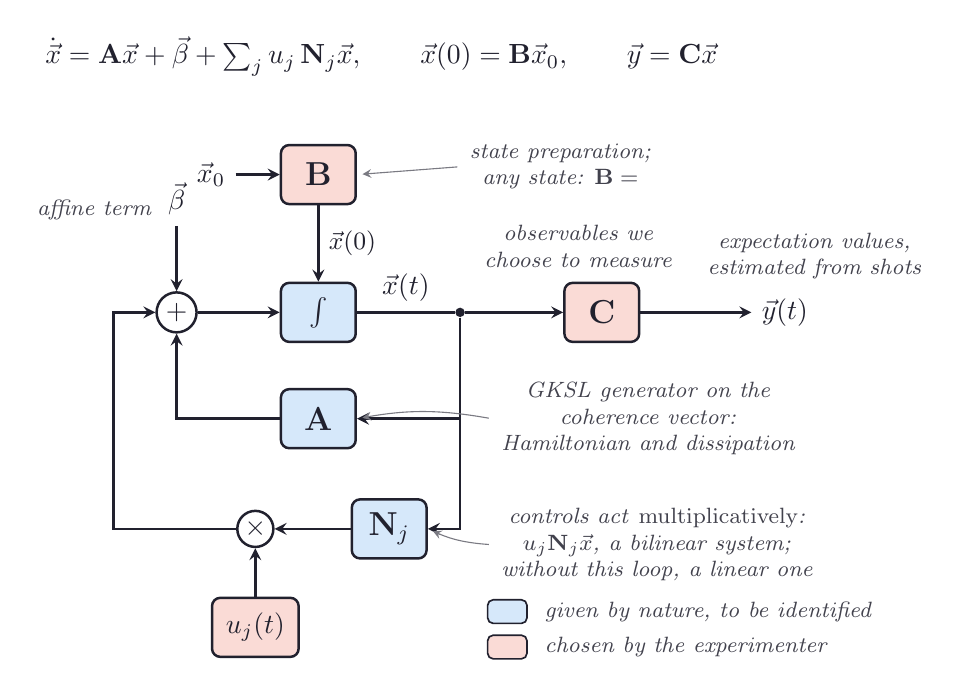
\begin{tikzpicture}[ink/.style={line width=0.9pt, ndInk}, faint/.style={line width=0.4pt, ndInk!35}, dashedink/.style={line width=0.5pt, ndInk!55, dash pattern=on 2.5pt off 2pt}, vec/.style={->, >=stealth, line width=1.2pt}, note/.style={font=\footnotesize\itshape, text=ndInk!85, align=center}, pointer/.style={->, >=stealth, line width=0.4pt, ndInk!60, shorten >=2pt, shorten <=1pt}, dot/.style={circle, fill=ndInk, inner sep=0pt, minimum size=3.4pt}, wash/.style={fill=ndSky, fill opacity=0.55}, every node/.style={text=ndInk}]
\definecolor{ndInk}{rgb}{0.13,0.13,0.18}
\definecolor{ndPaper}{rgb}{0.99,0.96,0.88}
\definecolor{ndSky}{rgb}{0.84,0.91,0.98}
\definecolor{ndRose}{rgb}{0.98,0.86,0.84}
\definecolor{ndBlue}{rgb}{0.13,0.36,0.66}
\definecolor{ndRed}{rgb}{0.78,0.20,0.16}
\definecolor{ndGold}{rgb}{0.88,0.62,0.10}
\definecolor{ndGreen}{rgb}{0.18,0.52,0.30}
\node at (5.6,3.25) {$\dot{\vec x}=\mathbf A\vec x+\vec\beta+\sum_j u_j\,\mathbf N_j\vec x,\qquad \vec x(0)=\mathbf B\vec x_0,\qquad \vec y=\mathbf C\vec x$};
\node[circle, draw=ndInk, line width=0.9pt, inner sep=1.5pt, fill=white] (S) at (3.0,0) {$+$};
\node[draw=ndInk, line width=0.9pt, rounded corners=3pt, minimum width=0.95cm, minimum height=0.75cm, font=\large, fill=ndSky] (I) at (4.8,0) {$\int$};
\node[dot] (P) at (6.6,0) {};
\node[draw=ndInk, line width=0.9pt, rounded corners=3pt, minimum width=0.95cm, minimum height=0.75cm, font=\large, fill=ndRose] (C) at (8.4,0) {$\mathbf C$};
\node[draw=ndInk, line width=0.9pt, rounded corners=3pt, minimum width=0.95cm, minimum height=0.75cm, font=\large, fill=ndRose] (B) at (4.8,1.75) {$\mathbf B$};
\node[draw=ndInk, line width=0.9pt, rounded corners=3pt, minimum width=0.95cm, minimum height=0.75cm, font=\large, fill=ndSky] (A) at (4.8,-1.35) {$\mathbf A$};
\node[draw=ndInk, line width=0.9pt, rounded corners=3pt, minimum width=0.95cm, minimum height=0.75cm, font=\large, fill=ndSky] (Nj) at (5.7,-2.75) {$\mathbf N_j$};
\node[circle, draw=ndInk, line width=0.9pt, inner sep=1pt, fill=white] (M) at (4.0,-2.75) {$\times$};
\node[draw=ndInk, line width=0.9pt, rounded corners=3pt, minimum width=0.95cm, minimum height=0.75cm, font=\large, fill=ndRose, minimum width=1.1cm, font=\normalsize] (U) at (4.0,-4.0) {$u_j(t)$};
\draw[->, >=stealth, line width=0.9pt, ndInk] (S) -- (I);
\draw[line width=0.9pt, ndInk] (I) -- node[above] {$\vec x(t)$} (P);
\draw[->, >=stealth, line width=0.9pt, ndInk] (P) -- (C);
\draw[->, >=stealth, line width=0.9pt, ndInk] (C) -- (10.3,0) node[right] {$\vec y(t)$};
\draw[->, >=stealth, line width=0.9pt, ndInk] (3.75,1.75) node[left] {$\vec x_0$} -- (B);
\draw[->, >=stealth, line width=0.9pt, ndInk] (B) -- node[right, font=\small] {$\vec x(0)$} (I);
\draw[->, >=stealth, line width=0.9pt, ndInk] (3.0,1.1) node[above] {$\vec\beta$} -- (S);
\draw[->, >=stealth, line width=0.9pt, ndInk] (P) |- (A);
\draw[->, >=stealth, line width=0.9pt, ndInk] (A) -| (S);
\draw[->, >=stealth, line width=0.9pt, ndInk] (P) |- (Nj);
\draw[->, >=stealth, line width=0.9pt, ndInk] (Nj) -- (M);
\draw[->, >=stealth, line width=0.9pt, ndInk] (U) -- (M);
\draw[->, >=stealth, line width=0.9pt, ndInk] (M) -| (2.2,0) -- (S);
\node[note, anchor=west] (nB) at (6.6,1.85) {state preparation;\\ any state: $\mathbf B=\Id$};
\draw[pointer] (nB.west) -- (B.east);
\node[note, anchor=south] at (8.1,0.45) {observables we\\ choose to measure};
\node[note, anchor=south] at (11.1,0.3) {expectation values,\\ estimated from shots};
\node[note, anchor=west] (nA) at (7.0,-1.35) {GKSL generator on the\\ coherence vector:\\ Hamiltonian and dissipation};
\draw[pointer] (nA.west) to[bend right=10] (A.east);
\node[note, anchor=west] (nN) at (7.0,-2.95) {controls act \emph{multiplicatively}:\\ $u_j\mathbf N_j\vec x$, a bilinear system;\\ without this loop, a linear one};
\draw[pointer] (nN.west) to[bend left=10] (Nj.east);
\node[note, anchor=east] at (2.8,1.3) {affine term};
\node[draw=ndInk, line width=0.6pt, rounded corners=2pt, fill=ndRose, minimum width=0.5cm, minimum height=0.3cm] at (7.2,-4.25) {};
\node[note, anchor=west] at (7.55,-4.25) {chosen by the experimenter};
\node[draw=ndInk, line width=0.6pt, rounded corners=2pt, fill=ndSky, minimum width=0.5cm, minimum height=0.3cm] at (7.2,-3.8) {};
\node[note, anchor=west] at (7.55,-3.8) {given by nature, to be identified};
\end{tikzpicture}
}
\caption{The bilinear state-space model of an open quantum system as a block diagram. Rose: the blocks chosen by the experimenter, namely the preparation $\mathbf B$, the controls $u_j$ and the readout $\mathbf C$. Blue: the blocks given by nature and to be identified, namely the generator $\mathbf A$ with the affine term $\vec\beta$, and the coupling matrices $\mathbf N_j$, which are known once the controls are calibrated. Without the lower loop the model is linear. Generated by \texttt{code/ch04\_blockdiagram.py}.}\label{fig:ch04:blockdiagram}
\end{figure}}
\onp{\begin{center}\resizebox{!}{0.78\textheight}{% Generated by code/needham.py -- do not edit by hand.
\definecolor{qocA}{rgb}{0.00,0.45,0.70}
\definecolor{qocB}{rgb}{0.90,0.60,0.00}
\definecolor{qocC}{rgb}{0.00,0.62,0.45}
\definecolor{qocD}{rgb}{0.80,0.40,0.00}
\definecolor{qocE}{rgb}{0.80,0.60,0.70}
\definecolor{qocF}{rgb}{0.35,0.70,0.90}
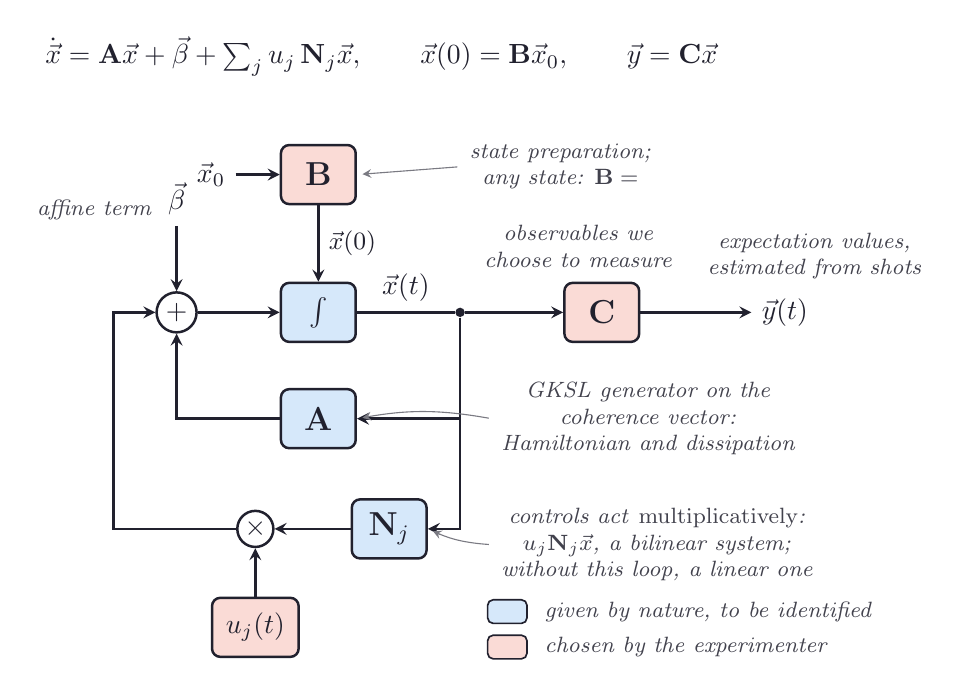
\begin{tikzpicture}[ink/.style={line width=0.9pt, ndInk}, faint/.style={line width=0.4pt, ndInk!35}, dashedink/.style={line width=0.5pt, ndInk!55, dash pattern=on 2.5pt off 2pt}, vec/.style={->, >=stealth, line width=1.2pt}, note/.style={font=\footnotesize\itshape, text=ndInk!85, align=center}, pointer/.style={->, >=stealth, line width=0.4pt, ndInk!60, shorten >=2pt, shorten <=1pt}, dot/.style={circle, fill=ndInk, inner sep=0pt, minimum size=3.4pt}, wash/.style={fill=ndSky, fill opacity=0.55}, every node/.style={text=ndInk}]
\definecolor{ndInk}{rgb}{0.13,0.13,0.18}
\definecolor{ndPaper}{rgb}{0.99,0.96,0.88}
\definecolor{ndSky}{rgb}{0.84,0.91,0.98}
\definecolor{ndRose}{rgb}{0.98,0.86,0.84}
\definecolor{ndBlue}{rgb}{0.13,0.36,0.66}
\definecolor{ndRed}{rgb}{0.78,0.20,0.16}
\definecolor{ndGold}{rgb}{0.88,0.62,0.10}
\definecolor{ndGreen}{rgb}{0.18,0.52,0.30}
\node at (5.6,3.25) {$\dot{\vec x}=\mathbf A\vec x+\vec\beta+\sum_j u_j\,\mathbf N_j\vec x,\qquad \vec x(0)=\mathbf B\vec x_0,\qquad \vec y=\mathbf C\vec x$};
\node[circle, draw=ndInk, line width=0.9pt, inner sep=1.5pt, fill=white] (S) at (3.0,0) {$+$};
\node[draw=ndInk, line width=0.9pt, rounded corners=3pt, minimum width=0.95cm, minimum height=0.75cm, font=\large, fill=ndSky] (I) at (4.8,0) {$\int$};
\node[dot] (P) at (6.6,0) {};
\node[draw=ndInk, line width=0.9pt, rounded corners=3pt, minimum width=0.95cm, minimum height=0.75cm, font=\large, fill=ndRose] (C) at (8.4,0) {$\mathbf C$};
\node[draw=ndInk, line width=0.9pt, rounded corners=3pt, minimum width=0.95cm, minimum height=0.75cm, font=\large, fill=ndRose] (B) at (4.8,1.75) {$\mathbf B$};
\node[draw=ndInk, line width=0.9pt, rounded corners=3pt, minimum width=0.95cm, minimum height=0.75cm, font=\large, fill=ndSky] (A) at (4.8,-1.35) {$\mathbf A$};
\node[draw=ndInk, line width=0.9pt, rounded corners=3pt, minimum width=0.95cm, minimum height=0.75cm, font=\large, fill=ndSky] (Nj) at (5.7,-2.75) {$\mathbf N_j$};
\node[circle, draw=ndInk, line width=0.9pt, inner sep=1pt, fill=white] (M) at (4.0,-2.75) {$\times$};
\node[draw=ndInk, line width=0.9pt, rounded corners=3pt, minimum width=0.95cm, minimum height=0.75cm, font=\large, fill=ndRose, minimum width=1.1cm, font=\normalsize] (U) at (4.0,-4.0) {$u_j(t)$};
\draw[->, >=stealth, line width=0.9pt, ndInk] (S) -- (I);
\draw[line width=0.9pt, ndInk] (I) -- node[above] {$\vec x(t)$} (P);
\draw[->, >=stealth, line width=0.9pt, ndInk] (P) -- (C);
\draw[->, >=stealth, line width=0.9pt, ndInk] (C) -- (10.3,0) node[right] {$\vec y(t)$};
\draw[->, >=stealth, line width=0.9pt, ndInk] (3.75,1.75) node[left] {$\vec x_0$} -- (B);
\draw[->, >=stealth, line width=0.9pt, ndInk] (B) -- node[right, font=\small] {$\vec x(0)$} (I);
\draw[->, >=stealth, line width=0.9pt, ndInk] (3.0,1.1) node[above] {$\vec\beta$} -- (S);
\draw[->, >=stealth, line width=0.9pt, ndInk] (P) |- (A);
\draw[->, >=stealth, line width=0.9pt, ndInk] (A) -| (S);
\draw[->, >=stealth, line width=0.9pt, ndInk] (P) |- (Nj);
\draw[->, >=stealth, line width=0.9pt, ndInk] (Nj) -- (M);
\draw[->, >=stealth, line width=0.9pt, ndInk] (U) -- (M);
\draw[->, >=stealth, line width=0.9pt, ndInk] (M) -| (2.2,0) -- (S);
\node[note, anchor=west] (nB) at (6.6,1.85) {state preparation;\\ any state: $\mathbf B=\Id$};
\draw[pointer] (nB.west) -- (B.east);
\node[note, anchor=south] at (8.1,0.45) {observables we\\ choose to measure};
\node[note, anchor=south] at (11.1,0.3) {expectation values,\\ estimated from shots};
\node[note, anchor=west] (nA) at (7.0,-1.35) {GKSL generator on the\\ coherence vector:\\ Hamiltonian and dissipation};
\draw[pointer] (nA.west) to[bend right=10] (A.east);
\node[note, anchor=west] (nN) at (7.0,-2.95) {controls act \emph{multiplicatively}:\\ $u_j\mathbf N_j\vec x$, a bilinear system;\\ without this loop, a linear one};
\draw[pointer] (nN.west) to[bend left=10] (Nj.east);
\node[note, anchor=east] at (2.8,1.3) {affine term};
\node[draw=ndInk, line width=0.6pt, rounded corners=2pt, fill=ndRose, minimum width=0.5cm, minimum height=0.3cm] at (7.2,-4.25) {};
\node[note, anchor=west] at (7.55,-4.25) {chosen by the experimenter};
\node[draw=ndInk, line width=0.6pt, rounded corners=2pt, fill=ndSky, minimum width=0.5cm, minimum height=0.3cm] at (7.2,-3.8) {};
\node[note, anchor=west] at (7.55,-3.8) {given by nature, to be identified};
\end{tikzpicture}
}\end{center}}
\end{frame}

\begin{frame}\ft{Controllability and observability}
\begin{defn}[Controllability]\label{def:ch04:controllability}
A system \eqref{eq:ch04:LDS} is controllable if for any given initial state $\vec x_0$ and final state $\vec{x}_{1}$ there exists a control $\vec u(\cdot) : [0, t] \rightarrow \R^{m}$ such that $\vec{x}(t) = \vec{x}_1$.
\end{defn}
\begin{defn}[Observability]\label{def:ch04:observability}
A system \eqref{eq:ch04:LDS} is observable if for a given input $\vec u(\cdot)$ and output $\vec y(\cdot)$ on $[0,t]$ one can uniquely determine the initial state $\vec x(0)$.
\end{defn}
\ona{These concepts are prerequisites for identifiability and both are required to be satisfied for identifiability to hold. Controllability ensures that every degree of freedom of the state can be reached from an arbitrary admissible input, in order that the system parameters can influence the dynamics. Without this, regardless of experimental design, system parameters governing an unreachable subspace can never be excited and hence will not appear in the output trajectory. Similarly, the dual requirement of observability ensures that every degree of freedom leaves a trace in the measured output. Systems that satisfy both properties are referred to as \emph{minimal} \citep{Sarachik_1997}.}
\onp{\begin{itemize}
    \item Controllability: every direction of the state can be excited by the inputs.
    \item Observability: every direction of the state leaves a trace in the outputs.
    \item Both together $=$ \alert{minimal} realisation, the prerequisite of identifiability.
\end{itemize}}
\end{frame}

\begin{frame}\ft{Kalman rank conditions}
\ona{A practical way to determine the controllability and observability of a system is to compute the rank of the corresponding controllability and observability matrices, $\CM \in \R^{n\times nm}$ and $\OM \in \R^{np \times n}$, respectively. These are defined as follows}
\onp{Test by rank:}
\begin{equation}\label{eq:ch04:OMCM}
        \OM^{(\text{lin})} = \begin{bmatrix}
            \mathbf{C} \\ \mathbf{CA} \\ \vdots \\ \mathbf{C}\mathbf{A}^{n-1}
        \end{bmatrix}\in\R^{np\times n}, \qquad
        \CM^{(\text{lin})} = \begin{bmatrix}
            \mathbf{B} & \mathbf{AB} & \cdots & \mathbf{A}^{n-1}\mathbf{B}
        \end{bmatrix}\in\R^{n\times nm}.
\end{equation}
\begin{thm}[Kalman]\label{thm:ch04:kalman}
System \eqref{eq:ch04:LDS} is controllable if and only if $\rank\CM^{(\mathrm{lin})}=n$, and observable if and only if $\rank\OM^{(\mathrm{lin})}=n$ \citep{KALMAN1960491,Antsaklis97}.
\end{thm}
\ona{\begin{pf}
(Observability.) With $\vec u\equiv0$ the output is $\vec y(t)=\mathbf C\ee^{\mathbf At}\vec x(0)$. Differentiating $k$ times at $t=0$ gives $\vec y^{(k)}(0)=\mathbf C\mathbf A^{k}\vec x(0)$, so the output determines $\OM^{(\mathrm{lin})}\vec x(0)$; by Cayley--Hamilton, powers $\mathbf A^{k}$ with $k\ge n$ are linear combinations of lower powers, so nothing more is determined. The map $\vec x(0)\mapsto \vec y(\cdot)$ is therefore injective iff $\OM^{(\mathrm{lin})}$ has trivial kernel. (Controllability.) The reachable set from $0$ is $\{\int_0^t\ee^{\mathbf A(t-s)}\mathbf B\vec u(s)\,\mathrm{d}s\}$, which by the same Cayley--Hamilton argument is the column space of $\CM^{(\mathrm{lin})}$. With nonzero inputs one shifts by $\ee^{\mathbf At}\vec x_0$.
\end{pf}
Note that, if the initial state may be arbitrary and $n=p$, the matrix $\mathbf B$ may be taken to be the identity. This leads to controllability being trivially satisfied. Observe also the duality: $(\mathbf A,\mathbf C)$ is observable iff $(\mathbf A^{\top},\mathbf C^{\top})$ is controllable, since $\OM^{(\mathrm{lin})}(\mathbf A,\mathbf C)^{\top}=\CM^{(\mathrm{lin})}(\mathbf A^\top,\mathbf C^\top)$.}
\onp{\begin{itemize}
    \item Proof idea: $\vec y^{(k)}(0)=\mathbf C\mathbf A^k\vec x(0)$; Cayley--Hamilton stops at $k=n-1$.
    \item Arbitrary state preparation $\Leftrightarrow$ $\mathbf B=\Id$ $\Rightarrow$ controllability for free.
    \item Duality: $(\mathbf A,\mathbf C)$ observable $\Leftrightarrow$ $(\mathbf A^\top,\mathbf C^\top)$ controllable.
\end{itemize}}
\end{frame}

\begin{frame}\ft{Reachable and unobservable subspaces}
\ona{Figure~\ref{fig:ch04:kalman} shows the two rank conditions as subspaces of a three-dimensional state space. The column space of $\CM^{(\mathrm{lin})}$ is the set of states that the inputs can reach from rest. Here it is a plane, and no input can push the state off it. The kernel of $\OM^{(\mathrm{lin})}$ is the set of directions that leave no trace in the output. Here it is a line, and two initial states that differ along it produce exactly the same data. Controllability fails when the plane is not the whole space, and observability when the line is not just the origin. Data can only ever reveal the part of the system that is both reachable and observable, which is the minimal realisation of Theorem~\ref{thm:ch04:similarity}; here it is two-dimensional.}
\ona{\begin{figure}[H]\centering
\resizebox{\linewidth}{!}{% Generated by code/needham.py -- do not edit by hand.
\definecolor{qocA}{rgb}{0.00,0.45,0.70}
\definecolor{qocB}{rgb}{0.90,0.60,0.00}
\definecolor{qocC}{rgb}{0.00,0.62,0.45}
\definecolor{qocD}{rgb}{0.80,0.40,0.00}
\definecolor{qocE}{rgb}{0.80,0.60,0.70}
\definecolor{qocF}{rgb}{0.35,0.70,0.90}
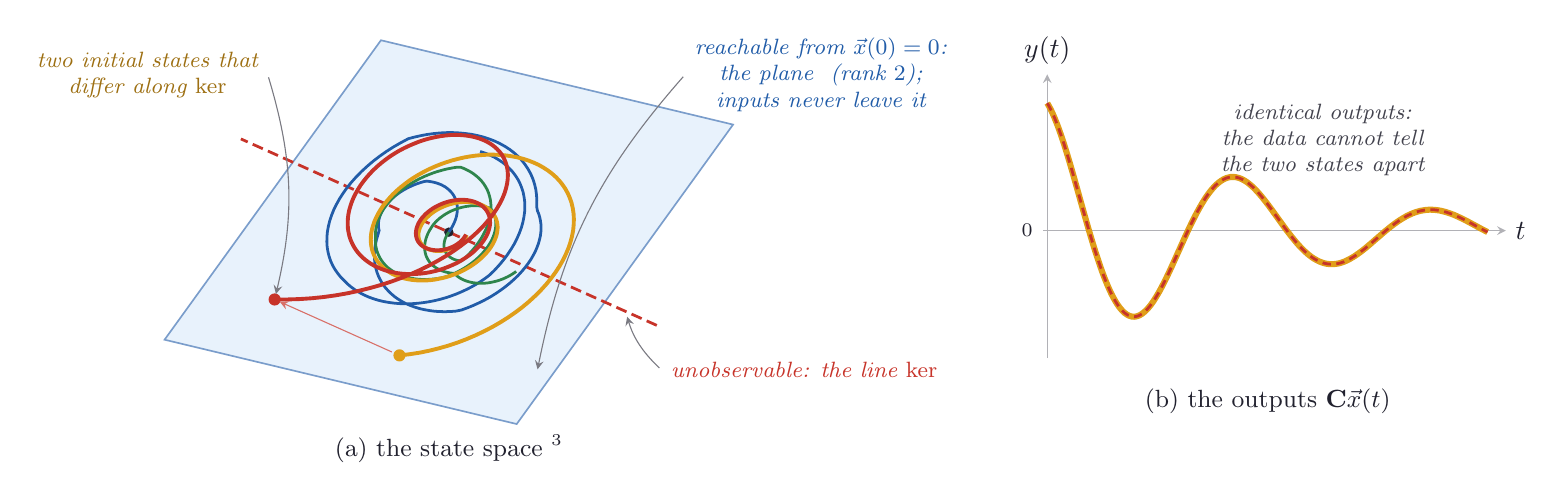
\begin{tikzpicture}[ink/.style={line width=0.9pt, ndInk}, faint/.style={line width=0.4pt, ndInk!35}, dashedink/.style={line width=0.5pt, ndInk!55, dash pattern=on 2.5pt off 2pt}, vec/.style={->, >=stealth, line width=1.2pt}, note/.style={font=\footnotesize\itshape, text=ndInk!85, align=center}, pointer/.style={->, >=stealth, line width=0.4pt, ndInk!60, shorten >=2pt, shorten <=1pt}, dot/.style={circle, fill=ndInk, inner sep=0pt, minimum size=3.4pt}, wash/.style={fill=ndSky, fill opacity=0.55}, every node/.style={text=ndInk}]
\definecolor{ndInk}{rgb}{0.13,0.13,0.18}
\definecolor{ndPaper}{rgb}{0.99,0.96,0.88}
\definecolor{ndSky}{rgb}{0.84,0.91,0.98}
\definecolor{ndRose}{rgb}{0.98,0.86,0.84}
\definecolor{ndBlue}{rgb}{0.13,0.36,0.66}
\definecolor{ndRed}{rgb}{0.78,0.20,0.16}
\definecolor{ndGold}{rgb}{0.88,0.62,0.10}
\definecolor{ndGreen}{rgb}{0.18,0.52,0.30}
\filldraw[fill=ndSky, fill opacity=0.55, draw=ndBlue!60, line width=0.6pt] (-0.862,2.437) -- (-3.610,-1.366) -- (0.862,-2.437) -- (3.610,1.366) -- cycle;
\draw[line width=1.0pt, ndRed, dash pattern=on 4pt off 2pt] (2.641,-1.184) -- (-2.641,1.184);
\node[dot] at (0.000,0.000) {};
\draw[line width=1.0pt, ndBlue] (0.000,0.000) -- (0.022,0.033) -- (0.042,0.066) -- (0.059,0.099) -- (0.074,0.132) -- (0.086,0.164) -- (0.096,0.197) -- (0.102,0.228) -- (0.107,0.260) -- (0.108,0.290) -- (0.108,0.320) -- (0.104,0.349) -- (0.099,0.377) -- (0.091,0.404) -- (0.080,0.430) -- (0.068,0.455) -- (0.054,0.478) -- (0.037,0.500) -- (0.018,0.521) -- (-0.002,0.540) -- (-0.024,0.558) -- (-0.047,0.575) -- (-0.072,0.589) -- (-0.099,0.603) -- (-0.127,0.614) -- (-0.155,0.624) -- (-0.185,0.632) -- (-0.216,0.639) -- (-0.247,0.644) -- (-0.279,0.648) -- (-0.317,0.642) -- (-0.358,0.630) -- (-0.397,0.617) -- (-0.436,0.603) -- (-0.474,0.586) -- (-0.511,0.569) -- (-0.547,0.550) -- (-0.581,0.531) -- (-0.614,0.510) -- (-0.645,0.488) -- (-0.675,0.466) -- (-0.703,0.442) -- (-0.730,0.418) -- (-0.754,0.394) -- (-0.777,0.368) -- (-0.798,0.343) -- (-0.816,0.317) -- (-0.833,0.291) -- (-0.848,0.266) -- (-0.861,0.240) -- (-0.872,0.214) -- (-0.880,0.188) -- (-0.887,0.163) -- (-0.891,0.138) -- (-0.894,0.114) -- (-0.895,0.090) -- (-0.893,0.067) -- (-0.890,0.044) -- (-0.885,0.022) -- (-0.899,-0.028) -- (-0.918,-0.093) -- (-0.932,-0.157) -- (-0.941,-0.220) -- (-0.945,-0.281) -- (-0.944,-0.342) -- (-0.938,-0.400) -- (-0.928,-0.456) -- (-0.912,-0.511) -- (-0.892,-0.563) -- (-0.867,-0.613) -- (-0.839,-0.660) -- (-0.806,-0.705) -- (-0.769,-0.746) -- (-0.729,-0.785) -- (-0.685,-0.822) -- (-0.638,-0.855) -- (-0.588,-0.885) -- (-0.536,-0.911) -- (-0.480,-0.935) -- (-0.423,-0.955) -- (-0.363,-0.973) -- (-0.302,-0.986) -- (-0.239,-0.997) -- (-0.175,-1.005) -- (-0.110,-1.009) -- (-0.044,-1.010) -- (0.022,-1.008) -- (0.089,-1.003) -- (0.160,-0.989) -- (0.237,-0.961) -- (0.313,-0.930) -- (0.387,-0.896) -- (0.459,-0.860) -- (0.528,-0.822) -- (0.594,-0.781) -- (0.657,-0.738) -- (0.717,-0.694) -- (0.774,-0.648) -- (0.828,-0.600) -- (0.878,-0.552) -- (0.924,-0.502) -- (0.966,-0.452) -- (1.005,-0.401) -- (1.040,-0.350) -- (1.070,-0.298) -- (1.097,-0.247) -- (1.119,-0.196) -- (1.138,-0.145) -- (1.152,-0.094) -- (1.163,-0.045) -- (1.169,0.004) -- (1.171,0.052) -- (1.170,0.098) -- (1.164,0.143) -- (1.155,0.187) -- (1.143,0.229) -- (1.126,0.269) -- (1.116,0.321) -- (1.118,0.396) -- (1.114,0.469) -- (1.105,0.540) -- (1.089,0.609) -- (1.068,0.675) -- (1.041,0.738) -- (1.008,0.798) -- (0.971,0.855) -- (0.929,0.909) -- (0.882,0.959) -- (0.830,1.006) -- (0.775,1.049) -- (0.715,1.088) -- (0.652,1.123) -- (0.586,1.155) -- (0.517,1.182) -- (0.445,1.206) -- (0.371,1.225) -- (0.294,1.241) -- (0.216,1.252) -- (0.136,1.260) -- (0.056,1.264) -- (-0.026,1.264) -- (-0.108,1.260) -- (-0.190,1.252) -- (-0.272,1.241) -- (-0.353,1.226) -- (-0.434,1.208) -- (-0.514,1.187) -- (-0.611,1.135) -- (-0.705,1.081) -- (-0.794,1.024) -- (-0.879,0.964) -- (-0.960,0.902) -- (-1.036,0.837) -- (-1.108,0.771) -- (-1.174,0.704) -- (-1.236,0.635) -- (-1.292,0.566) -- (-1.342,0.495) -- (-1.388,0.424) -- (-1.427,0.353) -- (-1.462,0.283) -- (-1.490,0.212) -- (-1.513,0.142) -- (-1.530,0.073) -- (-1.542,0.006) -- (-1.548,-0.061) -- (-1.549,-0.126) -- (-1.545,-0.189) -- (-1.535,-0.250) -- (-1.520,-0.310) -- (-1.501,-0.366) -- (-1.476,-0.421) -- (-1.447,-0.472) -- (-1.413,-0.521) -- (-1.376,-0.567) -- (-1.334,-0.610) -- (-1.291,-0.654) -- (-1.244,-0.694) -- (-1.193,-0.731) -- (-1.139,-0.765) -- (-1.082,-0.795) -- (-1.023,-0.822) -- (-0.960,-0.845) -- (-0.896,-0.865) -- (-0.829,-0.881) -- (-0.761,-0.893) -- (-0.691,-0.902) -- (-0.620,-0.908) -- (-0.548,-0.910) -- (-0.476,-0.909) -- (-0.403,-0.904) -- (-0.330,-0.896) -- (-0.257,-0.885) -- (-0.185,-0.871) -- (-0.114,-0.854) -- (-0.043,-0.834) -- (0.026,-0.811) -- (0.094,-0.786) -- (0.160,-0.758) -- (0.225,-0.728) -- (0.287,-0.696) -- (0.347,-0.662) -- (0.405,-0.626) -- (0.460,-0.588) -- (0.512,-0.549) -- (0.573,-0.491) -- (0.635,-0.424) -- (0.692,-0.356) -- (0.744,-0.287) -- (0.790,-0.218) -- (0.832,-0.148) -- (0.867,-0.078) -- (0.897,-0.009) -- (0.922,0.060) -- (0.941,0.128) -- (0.954,0.195) -- (0.963,0.261) -- (0.965,0.326) -- (0.963,0.389) -- (0.955,0.450) -- (0.943,0.509) -- (0.925,0.565) -- (0.903,0.620) -- (0.876,0.672) -- (0.844,0.721) -- (0.809,0.767) -- (0.769,0.810) -- (0.726,0.851) -- (0.679,0.888) -- (0.628,0.922) -- (0.575,0.953) -- (0.518,0.980) -- (0.460,1.004) -- (0.398,1.025);
\draw[line width=1.0pt, ndGreen] (0.000,0.000) -- (-0.013,-0.019) -- (-0.024,-0.037) -- (-0.034,-0.056) -- (-0.042,-0.075) -- (-0.049,-0.093) -- (-0.054,-0.111) -- (-0.058,-0.129) -- (-0.060,-0.147) -- (-0.061,-0.164) -- (-0.061,-0.181) -- (-0.059,-0.198) -- (-0.056,-0.214) -- (-0.051,-0.229) -- (-0.046,-0.243) -- (-0.039,-0.257) -- (-0.030,-0.271) -- (-0.021,-0.283) -- (-0.010,-0.295) -- (0.001,-0.306) -- (0.013,-0.316) -- (0.027,-0.325) -- (0.041,-0.334) -- (0.056,-0.341) -- (0.072,-0.348) -- (0.088,-0.353) -- (0.105,-0.358) -- (0.122,-0.362) -- (0.140,-0.365) -- (0.158,-0.367) -- (0.199,-0.335) -- (0.249,-0.286) -- (0.295,-0.236) -- (0.337,-0.185) -- (0.375,-0.134) -- (0.409,-0.082) -- (0.439,-0.030) -- (0.465,0.022) -- (0.487,0.073) -- (0.505,0.125) -- (0.519,0.175) -- (0.528,0.225) -- (0.534,0.274) -- (0.536,0.322) -- (0.533,0.369) -- (0.527,0.414) -- (0.517,0.457) -- (0.504,0.499) -- (0.487,0.540) -- (0.466,0.578) -- (0.443,0.614) -- (0.416,0.649) -- (0.386,0.681) -- (0.353,0.710) -- (0.318,0.738) -- (0.280,0.763) -- (0.240,0.785) -- (0.198,0.806) -- (0.154,0.823) -- (0.098,0.824) -- (0.037,0.814) -- (-0.024,0.802) -- (-0.084,0.787) -- (-0.143,0.770) -- (-0.201,0.751) -- (-0.258,0.729) -- (-0.314,0.706) -- (-0.368,0.680) -- (-0.420,0.653) -- (-0.470,0.624) -- (-0.519,0.594) -- (-0.565,0.562) -- (-0.608,0.529) -- (-0.650,0.494) -- (-0.688,0.459) -- (-0.724,0.423) -- (-0.758,0.386) -- (-0.788,0.349) -- (-0.816,0.312) -- (-0.841,0.274) -- (-0.862,0.236) -- (-0.881,0.198) -- (-0.897,0.160) -- (-0.909,0.122) -- (-0.919,0.085) -- (-0.926,0.049) -- (-0.930,0.013) -- (-0.931,-0.022) -- (-0.931,-0.059) -- (-0.933,-0.102) -- (-0.931,-0.144) -- (-0.926,-0.185) -- (-0.917,-0.224) -- (-0.905,-0.262) -- (-0.890,-0.298) -- (-0.872,-0.332) -- (-0.851,-0.365) -- (-0.827,-0.396) -- (-0.801,-0.425) -- (-0.772,-0.452) -- (-0.740,-0.476) -- (-0.707,-0.499) -- (-0.671,-0.519) -- (-0.633,-0.537) -- (-0.594,-0.553) -- (-0.553,-0.567) -- (-0.511,-0.578) -- (-0.467,-0.587) -- (-0.423,-0.594) -- (-0.377,-0.599) -- (-0.332,-0.601) -- (-0.285,-0.601) -- (-0.238,-0.599) -- (-0.192,-0.595) -- (-0.145,-0.589) -- (-0.098,-0.581) -- (-0.052,-0.571) -- (-0.005,-0.556) -- (0.045,-0.536) -- (0.093,-0.513) -- (0.139,-0.489) -- (0.184,-0.464) -- (0.227,-0.437) -- (0.268,-0.409) -- (0.307,-0.380) -- (0.344,-0.350) -- (0.378,-0.318) -- (0.410,-0.287) -- (0.440,-0.254) -- (0.467,-0.221) -- (0.492,-0.188) -- (0.514,-0.154) -- (0.534,-0.121) -- (0.551,-0.087) -- (0.565,-0.053) -- (0.577,-0.020) -- (0.586,0.013) -- (0.592,0.045) -- (0.596,0.077) -- (0.597,0.108) -- (0.595,0.138) -- (0.591,0.167) -- (0.585,0.196) -- (0.576,0.223) -- (0.565,0.249) -- (0.552,0.274) -- (0.536,0.298) -- (0.511,0.307) -- (0.484,0.316) -- (0.456,0.323) -- (0.428,0.328) -- (0.399,0.332) -- (0.369,0.335) -- (0.339,0.336) -- (0.309,0.335) -- (0.279,0.334) -- (0.248,0.330) -- (0.218,0.326) -- (0.188,0.320) -- (0.158,0.313) -- (0.129,0.305) -- (0.100,0.296) -- (0.071,0.285) -- (0.044,0.274) -- (0.017,0.262) -- (-0.009,0.248) -- (-0.034,0.234) -- (-0.058,0.219) -- (-0.081,0.203) -- (-0.103,0.187) -- (-0.124,0.170) -- (-0.143,0.153) -- (-0.162,0.135) -- (-0.178,0.117) -- (-0.194,0.099) -- (-0.208,0.080) -- (-0.228,0.049) -- (-0.247,0.019) -- (-0.263,-0.012) -- (-0.276,-0.043) -- (-0.287,-0.073) -- (-0.296,-0.104) -- (-0.302,-0.133) -- (-0.306,-0.163) -- (-0.307,-0.191) -- (-0.306,-0.219) -- (-0.303,-0.246) -- (-0.297,-0.272) -- (-0.290,-0.297) -- (-0.280,-0.321) -- (-0.268,-0.344) -- (-0.254,-0.366) -- (-0.239,-0.387) -- (-0.221,-0.406) -- (-0.202,-0.424) -- (-0.181,-0.440) -- (-0.159,-0.455) -- (-0.135,-0.469) -- (-0.111,-0.481) -- (-0.085,-0.492) -- (-0.058,-0.501) -- (-0.030,-0.509) -- (-0.001,-0.515) -- (0.028,-0.520) -- (0.058,-0.523) -- (0.081,-0.536) -- (0.101,-0.554) -- (0.122,-0.570) -- (0.145,-0.585) -- (0.169,-0.598) -- (0.195,-0.610) -- (0.221,-0.620) -- (0.249,-0.629) -- (0.277,-0.636) -- (0.307,-0.642) -- (0.337,-0.646) -- (0.367,-0.649) -- (0.398,-0.650) -- (0.429,-0.649) -- (0.460,-0.648) -- (0.492,-0.645) -- (0.523,-0.640) -- (0.554,-0.634) -- (0.585,-0.627) -- (0.615,-0.619) -- (0.645,-0.609) -- (0.674,-0.599) -- (0.703,-0.587) -- (0.731,-0.574) -- (0.758,-0.561) -- (0.784,-0.546) -- (0.809,-0.531) -- (0.833,-0.515) -- (0.855,-0.498);
\draw[line width=1.4pt, ndGold] (-0.627,-1.565) -- (-0.502,-1.551) -- (-0.378,-1.532) -- (-0.255,-1.507) -- (-0.132,-1.477) -- (-0.012,-1.443) -- (0.106,-1.404) -- (0.222,-1.360) -- (0.335,-1.312) -- (0.445,-1.260) -- (0.551,-1.205) -- (0.653,-1.146) -- (0.751,-1.084) -- (0.845,-1.019) -- (0.934,-0.952) -- (1.018,-0.882) -- (1.096,-0.810) -- (1.169,-0.737) -- (1.237,-0.662) -- (1.299,-0.586) -- (1.355,-0.510) -- (1.405,-0.433) -- (1.449,-0.356) -- (1.487,-0.278) -- (1.519,-0.202) -- (1.545,-0.125) -- (1.565,-0.050) -- (1.579,0.024) -- (1.586,0.097) -- (1.588,0.168) -- (1.584,0.237) -- (1.574,0.304) -- (1.559,0.369) -- (1.538,0.431) -- (1.512,0.491) -- (1.481,0.548) -- (1.445,0.601) -- (1.405,0.652) -- (1.360,0.699) -- (1.311,0.743) -- (1.258,0.783) -- (1.201,0.820) -- (1.141,0.854) -- (1.078,0.883) -- (1.012,0.909) -- (0.944,0.931) -- (0.873,0.949) -- (0.801,0.963) -- (0.726,0.974) -- (0.651,0.981) -- (0.574,0.984) -- (0.497,0.984) -- (0.419,0.979) -- (0.342,0.972) -- (0.264,0.961) -- (0.187,0.947) -- (0.110,0.929) -- (0.034,0.909) -- (-0.040,0.885) -- (-0.113,0.859) -- (-0.184,0.830) -- (-0.253,0.799) -- (-0.320,0.765) -- (-0.385,0.729) -- (-0.447,0.691) -- (-0.507,0.651) -- (-0.563,0.609) -- (-0.617,0.566) -- (-0.667,0.522) -- (-0.714,0.477) -- (-0.757,0.430) -- (-0.797,0.383) -- (-0.834,0.336) -- (-0.866,0.288) -- (-0.895,0.239) -- (-0.920,0.191) -- (-0.942,0.143) -- (-0.959,0.095) -- (-0.973,0.048) -- (-0.983,0.002) -- (-0.989,-0.044) -- (-0.991,-0.089) -- (-0.990,-0.133) -- (-0.985,-0.175) -- (-0.977,-0.216) -- (-0.965,-0.255) -- (-0.950,-0.293) -- (-0.932,-0.329) -- (-0.911,-0.363) -- (-0.886,-0.396) -- (-0.859,-0.426) -- (-0.830,-0.454) -- (-0.797,-0.480) -- (-0.763,-0.504) -- (-0.726,-0.526) -- (-0.687,-0.545) -- (-0.647,-0.562) -- (-0.605,-0.576) -- (-0.561,-0.589) -- (-0.516,-0.598) -- (-0.470,-0.606) -- (-0.423,-0.611) -- (-0.376,-0.614) -- (-0.328,-0.614) -- (-0.279,-0.613) -- (-0.231,-0.609) -- (-0.182,-0.603) -- (-0.134,-0.594) -- (-0.086,-0.584) -- (-0.038,-0.572) -- (0.008,-0.558) -- (0.054,-0.542) -- (0.099,-0.525) -- (0.143,-0.506) -- (0.185,-0.485) -- (0.226,-0.463) -- (0.265,-0.440) -- (0.303,-0.415) -- (0.339,-0.390) -- (0.373,-0.363) -- (0.405,-0.336) -- (0.435,-0.308) -- (0.463,-0.279) -- (0.489,-0.250) -- (0.513,-0.220) -- (0.534,-0.190) -- (0.553,-0.160) -- (0.569,-0.130) -- (0.583,-0.100) -- (0.595,-0.070) -- (0.605,-0.041) -- (0.612,-0.011) -- (0.616,0.017) -- (0.619,0.046) -- (0.619,0.073) -- (0.616,0.100) -- (0.612,0.126) -- (0.605,0.151) -- (0.597,0.175) -- (0.586,0.198) -- (0.573,0.219) -- (0.559,0.240) -- (0.543,0.259) -- (0.525,0.277) -- (0.505,0.294) -- (0.484,0.309) -- (0.462,0.323) -- (0.438,0.336) -- (0.413,0.347) -- (0.387,0.357) -- (0.360,0.365) -- (0.332,0.371) -- (0.304,0.377) -- (0.275,0.380) -- (0.245,0.383) -- (0.215,0.384) -- (0.185,0.383) -- (0.155,0.381) -- (0.125,0.378) -- (0.094,0.373) -- (0.064,0.367) -- (0.035,0.360) -- (0.005,0.352) -- (-0.024,0.342) -- (-0.052,0.332) -- (-0.079,0.320) -- (-0.106,0.308) -- (-0.132,0.294) -- (-0.157,0.280) -- (-0.181,0.265) -- (-0.204,0.249) -- (-0.225,0.233) -- (-0.246,0.216) -- (-0.265,0.198) -- (-0.283,0.181) -- (-0.300,0.163) -- (-0.315,0.144) -- (-0.329,0.126) -- (-0.341,0.107) -- (-0.352,0.088) -- (-0.361,0.069) -- (-0.369,0.051) -- (-0.375,0.032) -- (-0.380,0.014) -- (-0.384,-0.004) -- (-0.386,-0.022) -- (-0.386,-0.039) -- (-0.385,-0.056) -- (-0.383,-0.073) -- (-0.380,-0.088) -- (-0.375,-0.104) -- (-0.368,-0.118) -- (-0.361,-0.132) -- (-0.352,-0.145) -- (-0.343,-0.158) -- (-0.332,-0.169) -- (-0.320,-0.180) -- (-0.307,-0.190) -- (-0.293,-0.199) -- (-0.279,-0.207) -- (-0.263,-0.214) -- (-0.247,-0.221) -- (-0.231,-0.226) -- (-0.214,-0.230) -- (-0.196,-0.234) -- (-0.178,-0.237) -- (-0.160,-0.238) -- (-0.141,-0.239) -- (-0.122,-0.239) -- (-0.104,-0.238) -- (-0.085,-0.237) -- (-0.066,-0.234) -- (-0.047,-0.231) -- (-0.028,-0.226) -- (-0.010,-0.221) -- (0.008,-0.216) -- (0.026,-0.209) -- (0.043,-0.202) -- (0.060,-0.195) -- (0.077,-0.187) -- (0.092,-0.178) -- (0.108,-0.169) -- (0.122,-0.159) -- (0.136,-0.149) -- (0.149,-0.139) -- (0.161,-0.128) -- (0.173,-0.117) -- (0.183,-0.106) -- (0.193,-0.094) -- (0.202,-0.083) -- (0.210,-0.071) -- (0.217,-0.059) -- (0.223,-0.047) -- (0.229,-0.036);
\draw[line width=1.4pt, ndRed] (-2.212,-0.855) -- (-2.054,-0.855) -- (-1.898,-0.850) -- (-1.743,-0.840) -- (-1.590,-0.824) -- (-1.439,-0.803) -- (-1.291,-0.777) -- (-1.146,-0.746) -- (-1.005,-0.711) -- (-0.867,-0.672) -- (-0.734,-0.629) -- (-0.605,-0.582) -- (-0.480,-0.532) -- (-0.361,-0.478) -- (-0.247,-0.422) -- (-0.139,-0.363) -- (-0.036,-0.302) -- (0.060,-0.240) -- (0.151,-0.175) -- (0.236,-0.110) -- (0.314,-0.043) -- (0.386,0.024) -- (0.451,0.092) -- (0.510,0.160) -- (0.562,0.228) -- (0.608,0.295) -- (0.647,0.362) -- (0.680,0.427) -- (0.706,0.491) -- (0.726,0.554) -- (0.740,0.616) -- (0.748,0.675) -- (0.750,0.732) -- (0.746,0.787) -- (0.736,0.839) -- (0.721,0.888) -- (0.701,0.935) -- (0.676,0.979) -- (0.646,1.019) -- (0.612,1.056) -- (0.574,1.090) -- (0.531,1.121) -- (0.485,1.148) -- (0.436,1.171) -- (0.383,1.191) -- (0.328,1.207) -- (0.270,1.219) -- (0.210,1.228) -- (0.148,1.233) -- (0.085,1.235) -- (0.020,1.233) -- (-0.046,1.227) -- (-0.112,1.218) -- (-0.179,1.205) -- (-0.246,1.190) -- (-0.313,1.171) -- (-0.379,1.149) -- (-0.444,1.123) -- (-0.509,1.095) -- (-0.572,1.065) -- (-0.634,1.032) -- (-0.694,0.996) -- (-0.752,0.958) -- (-0.807,0.918) -- (-0.861,0.876) -- (-0.912,0.832) -- (-0.960,0.787) -- (-1.005,0.740) -- (-1.047,0.692) -- (-1.086,0.643) -- (-1.122,0.594) -- (-1.154,0.543) -- (-1.183,0.492) -- (-1.209,0.441) -- (-1.230,0.390) -- (-1.248,0.338) -- (-1.263,0.287) -- (-1.274,0.236) -- (-1.281,0.186) -- (-1.284,0.137) -- (-1.284,0.088) -- (-1.281,0.041) -- (-1.273,-0.006) -- (-1.263,-0.051) -- (-1.249,-0.094) -- (-1.231,-0.136) -- (-1.211,-0.176) -- (-1.187,-0.215) -- (-1.160,-0.252) -- (-1.131,-0.286) -- (-1.099,-0.319) -- (-1.064,-0.349) -- (-1.027,-0.377) -- (-0.988,-0.403) -- (-0.946,-0.427) -- (-0.903,-0.448) -- (-0.858,-0.467) -- (-0.811,-0.484) -- (-0.763,-0.498) -- (-0.714,-0.509) -- (-0.664,-0.519) -- (-0.613,-0.526) -- (-0.562,-0.530) -- (-0.510,-0.533) -- (-0.458,-0.533) -- (-0.405,-0.530) -- (-0.353,-0.526) -- (-0.301,-0.519) -- (-0.250,-0.511) -- (-0.199,-0.500) -- (-0.149,-0.488) -- (-0.100,-0.473) -- (-0.052,-0.457) -- (-0.005,-0.439) -- (0.040,-0.420) -- (0.084,-0.400) -- (0.127,-0.378) -- (0.167,-0.354) -- (0.206,-0.330) -- (0.243,-0.305) -- (0.278,-0.279) -- (0.311,-0.252) -- (0.341,-0.224) -- (0.369,-0.196) -- (0.395,-0.168) -- (0.419,-0.139) -- (0.440,-0.110) -- (0.459,-0.081) -- (0.476,-0.052) -- (0.490,-0.023) -- (0.501,0.006) -- (0.510,0.034) -- (0.517,0.062) -- (0.522,0.089) -- (0.524,0.116) -- (0.523,0.142) -- (0.521,0.167) -- (0.516,0.191) -- (0.509,0.214) -- (0.500,0.236) -- (0.490,0.257) -- (0.477,0.277) -- (0.462,0.295) -- (0.446,0.313) -- (0.428,0.329) -- (0.409,0.343) -- (0.388,0.357) -- (0.366,0.368) -- (0.342,0.379) -- (0.318,0.388) -- (0.292,0.395) -- (0.266,0.401) -- (0.239,0.406) -- (0.211,0.409) -- (0.183,0.411) -- (0.154,0.411) -- (0.125,0.410) -- (0.096,0.407) -- (0.067,0.403) -- (0.038,0.398) -- (0.009,0.392) -- (-0.019,0.384) -- (-0.048,0.375) -- (-0.075,0.365) -- (-0.102,0.354) -- (-0.129,0.342) -- (-0.155,0.329) -- (-0.180,0.315) -- (-0.204,0.301) -- (-0.226,0.285) -- (-0.248,0.269) -- (-0.269,0.252) -- (-0.289,0.235) -- (-0.307,0.217) -- (-0.324,0.199) -- (-0.340,0.181) -- (-0.354,0.162) -- (-0.367,0.143) -- (-0.379,0.124) -- (-0.389,0.105) -- (-0.397,0.085) -- (-0.404,0.066) -- (-0.410,0.048) -- (-0.414,0.029) -- (-0.417,0.010) -- (-0.418,-0.008) -- (-0.418,-0.025) -- (-0.417,-0.042) -- (-0.414,-0.059) -- (-0.409,-0.075) -- (-0.404,-0.091) -- (-0.397,-0.105) -- (-0.389,-0.120) -- (-0.380,-0.133) -- (-0.369,-0.146) -- (-0.358,-0.157) -- (-0.346,-0.168) -- (-0.332,-0.178) -- (-0.318,-0.188) -- (-0.303,-0.196) -- (-0.287,-0.204) -- (-0.271,-0.210) -- (-0.254,-0.216) -- (-0.236,-0.220) -- (-0.218,-0.224) -- (-0.200,-0.227) -- (-0.181,-0.229) -- (-0.162,-0.230) -- (-0.143,-0.230) -- (-0.123,-0.230) -- (-0.104,-0.228) -- (-0.085,-0.226) -- (-0.065,-0.222) -- (-0.046,-0.218) -- (-0.028,-0.214) -- (-0.009,-0.208) -- (0.009,-0.202) -- (0.027,-0.195) -- (0.044,-0.188) -- (0.061,-0.180) -- (0.077,-0.171) -- (0.092,-0.162) -- (0.107,-0.152) -- (0.121,-0.142) -- (0.135,-0.132) -- (0.147,-0.122) -- (0.159,-0.111) -- (0.170,-0.100) -- (0.180,-0.088) -- (0.189,-0.077) -- (0.197,-0.065) -- (0.205,-0.054) -- (0.211,-0.042) -- (0.217,-0.030);
\node[dot, fill=ndGold, minimum size=4.4pt] at (-0.627,-1.565) {};
\node[dot, fill=ndRed, minimum size=4.4pt] at (-2.212,-0.855) {};
\draw[pointer, ndRed!70, shorten <=3pt] (-0.627,-1.565) -- (-2.212,-0.855);
\node[note, anchor=west, text=ndBlue] (pl) at (3.0,2.0) {reachable from $\vec x(0)=0$:\\ the plane $\ran\CM$ (rank $2$);\\ inputs never leave it};
\draw[pointer] (pl.west) to[bend right=15] (1.113,-1.811);
\node[note, anchor=west, text=ndRed] (ln) at (2.7,-1.75) {unobservable: the line $\ker\OM$};
\draw[pointer] (ln.west) to[bend left=15] (2.245,-1.007);
\node[note, anchor=east, text=ndGold!70!black] (st) at (-2.3,2.0) {two initial states that\\ differ along $\ker\OM$};
\draw[pointer] (st.east) to[bend left=15] (-2.212,-0.855);
\node[font=\small] at (0,-2.75) {(a) the state space $\R^3$};
\draw[faint, ->, >=stealth] (7.600,0.019) -- (13.424,0.019) node[right, text=ndInk] {$t$};
\draw[faint, ->, >=stealth] (7.600,-1.600) -- (7.600,2.004) node[above, text=ndInk] {$y(t)$};
\draw[faint] (7.660,0.019) -- (7.540,0.019) node[left, font=\scriptsize, text=ndInk] {$0$};
\draw[line width=2.2pt, ndGold] (7.600,1.638) -- (7.624,1.597) -- (7.648,1.550) -- (7.672,1.499) -- (7.696,1.443) -- (7.720,1.383) -- (7.744,1.320) -- (7.768,1.252) -- (7.792,1.181) -- (7.816,1.108) -- (7.840,1.031) -- (7.864,0.953) -- (7.888,0.872) -- (7.912,0.790) -- (7.936,0.706) -- (7.960,0.621) -- (7.984,0.536) -- (8.008,0.450) -- (8.032,0.364) -- (8.056,0.279) -- (8.080,0.194) -- (8.104,0.110) -- (8.128,0.027) -- (8.152,-0.054) -- (8.176,-0.134) -- (8.200,-0.212) -- (8.224,-0.287) -- (8.248,-0.360) -- (8.272,-0.431) -- (8.296,-0.498) -- (8.320,-0.563) -- (8.344,-0.624) -- (8.368,-0.681) -- (8.392,-0.736) -- (8.416,-0.786) -- (8.440,-0.832) -- (8.464,-0.875) -- (8.488,-0.914) -- (8.512,-0.948) -- (8.536,-0.978) -- (8.560,-1.005) -- (8.584,-1.027) -- (8.608,-1.044) -- (8.632,-1.058) -- (8.656,-1.067) -- (8.680,-1.073) -- (8.704,-1.074) -- (8.728,-1.071) -- (8.752,-1.064) -- (8.776,-1.054) -- (8.800,-1.039) -- (8.824,-1.021) -- (8.848,-1.000) -- (8.872,-0.975) -- (8.896,-0.948) -- (8.920,-0.917) -- (8.944,-0.883) -- (8.968,-0.846) -- (8.992,-0.807) -- (9.016,-0.766) -- (9.040,-0.723) -- (9.064,-0.677) -- (9.088,-0.630) -- (9.112,-0.582) -- (9.136,-0.532) -- (9.160,-0.481) -- (9.184,-0.429) -- (9.208,-0.376) -- (9.232,-0.323) -- (9.256,-0.269) -- (9.280,-0.216) -- (9.304,-0.162) -- (9.328,-0.109) -- (9.352,-0.056) -- (9.376,-0.004) -- (9.400,0.047) -- (9.424,0.097) -- (9.448,0.146) -- (9.472,0.194) -- (9.496,0.240) -- (9.520,0.284) -- (9.544,0.327) -- (9.568,0.368) -- (9.592,0.407) -- (9.616,0.444) -- (9.640,0.478) -- (9.664,0.510) -- (9.688,0.540) -- (9.712,0.568) -- (9.736,0.593) -- (9.760,0.615) -- (9.784,0.635) -- (9.808,0.652) -- (9.832,0.667) -- (9.856,0.679) -- (9.880,0.689) -- (9.904,0.695) -- (9.928,0.700) -- (9.952,0.701) -- (9.976,0.700) -- (10.000,0.697) -- (10.024,0.691) -- (10.048,0.683) -- (10.072,0.673) -- (10.096,0.660) -- (10.120,0.646) -- (10.144,0.629) -- (10.168,0.610) -- (10.192,0.590) -- (10.216,0.568) -- (10.240,0.544) -- (10.264,0.519) -- (10.288,0.492) -- (10.312,0.464) -- (10.336,0.435) -- (10.360,0.405) -- (10.384,0.374) -- (10.408,0.343) -- (10.432,0.310) -- (10.456,0.278) -- (10.480,0.244) -- (10.504,0.211) -- (10.528,0.178) -- (10.552,0.144) -- (10.576,0.111) -- (10.600,0.078) -- (10.624,0.045) -- (10.648,0.013) -- (10.672,-0.018) -- (10.696,-0.049) -- (10.720,-0.079) -- (10.744,-0.108) -- (10.768,-0.137) -- (10.792,-0.164) -- (10.816,-0.190) -- (10.840,-0.214) -- (10.864,-0.238) -- (10.888,-0.260) -- (10.912,-0.281) -- (10.936,-0.300) -- (10.960,-0.318) -- (10.984,-0.334) -- (11.008,-0.348) -- (11.032,-0.361) -- (11.056,-0.373) -- (11.080,-0.382) -- (11.104,-0.391) -- (11.128,-0.397) -- (11.152,-0.402) -- (11.176,-0.405) -- (11.200,-0.407) -- (11.224,-0.407) -- (11.248,-0.405) -- (11.272,-0.402) -- (11.296,-0.398) -- (11.320,-0.392) -- (11.344,-0.384) -- (11.368,-0.376) -- (11.392,-0.366) -- (11.416,-0.354) -- (11.440,-0.342) -- (11.464,-0.328) -- (11.488,-0.314) -- (11.512,-0.299) -- (11.536,-0.282) -- (11.560,-0.265) -- (11.584,-0.247) -- (11.608,-0.229) -- (11.632,-0.210) -- (11.656,-0.190) -- (11.680,-0.170) -- (11.704,-0.150) -- (11.728,-0.129) -- (11.752,-0.108) -- (11.776,-0.087) -- (11.800,-0.067) -- (11.824,-0.046) -- (11.848,-0.025) -- (11.872,-0.005) -- (11.896,0.016) -- (11.920,0.035) -- (11.944,0.055) -- (11.968,0.074) -- (11.992,0.092) -- (12.016,0.110) -- (12.040,0.127) -- (12.064,0.144) -- (12.088,0.159) -- (12.112,0.174) -- (12.136,0.188) -- (12.160,0.202) -- (12.184,0.214) -- (12.208,0.225) -- (12.232,0.236) -- (12.256,0.245) -- (12.280,0.254) -- (12.304,0.261) -- (12.328,0.268) -- (12.352,0.273) -- (12.376,0.277) -- (12.400,0.281) -- (12.424,0.283) -- (12.448,0.285) -- (12.472,0.285) -- (12.496,0.284) -- (12.520,0.283) -- (12.544,0.280) -- (12.568,0.277) -- (12.592,0.273) -- (12.616,0.267) -- (12.640,0.261) -- (12.664,0.255) -- (12.688,0.247) -- (12.712,0.239) -- (12.736,0.230) -- (12.760,0.221) -- (12.784,0.211) -- (12.808,0.200) -- (12.832,0.189) -- (12.856,0.178) -- (12.880,0.166) -- (12.904,0.154) -- (12.928,0.142) -- (12.952,0.129) -- (12.976,0.116) -- (13.000,0.103) -- (13.024,0.090) -- (13.048,0.077) -- (13.072,0.064) -- (13.096,0.051) -- (13.120,0.038) -- (13.144,0.026) -- (13.168,0.013) -- (13.192,0.001);
\draw[line width=1.0pt, ndRed, dash pattern=on 3pt off 2pt] (7.600,1.638) -- (7.624,1.597) -- (7.648,1.550) -- (7.672,1.499) -- (7.696,1.443) -- (7.720,1.383) -- (7.744,1.320) -- (7.768,1.252) -- (7.792,1.181) -- (7.816,1.108) -- (7.840,1.031) -- (7.864,0.953) -- (7.888,0.872) -- (7.912,0.790) -- (7.936,0.706) -- (7.960,0.621) -- (7.984,0.536) -- (8.008,0.450) -- (8.032,0.364) -- (8.056,0.279) -- (8.080,0.194) -- (8.104,0.110) -- (8.128,0.027) -- (8.152,-0.054) -- (8.176,-0.134) -- (8.200,-0.212) -- (8.224,-0.287) -- (8.248,-0.360) -- (8.272,-0.431) -- (8.296,-0.498) -- (8.320,-0.563) -- (8.344,-0.624) -- (8.368,-0.681) -- (8.392,-0.736) -- (8.416,-0.786) -- (8.440,-0.832) -- (8.464,-0.875) -- (8.488,-0.914) -- (8.512,-0.948) -- (8.536,-0.978) -- (8.560,-1.005) -- (8.584,-1.027) -- (8.608,-1.044) -- (8.632,-1.058) -- (8.656,-1.067) -- (8.680,-1.073) -- (8.704,-1.074) -- (8.728,-1.071) -- (8.752,-1.064) -- (8.776,-1.054) -- (8.800,-1.039) -- (8.824,-1.021) -- (8.848,-1.000) -- (8.872,-0.975) -- (8.896,-0.948) -- (8.920,-0.917) -- (8.944,-0.883) -- (8.968,-0.846) -- (8.992,-0.807) -- (9.016,-0.766) -- (9.040,-0.723) -- (9.064,-0.677) -- (9.088,-0.630) -- (9.112,-0.582) -- (9.136,-0.532) -- (9.160,-0.481) -- (9.184,-0.429) -- (9.208,-0.376) -- (9.232,-0.323) -- (9.256,-0.269) -- (9.280,-0.216) -- (9.304,-0.162) -- (9.328,-0.109) -- (9.352,-0.056) -- (9.376,-0.004) -- (9.400,0.047) -- (9.424,0.097) -- (9.448,0.146) -- (9.472,0.194) -- (9.496,0.240) -- (9.520,0.284) -- (9.544,0.327) -- (9.568,0.368) -- (9.592,0.407) -- (9.616,0.444) -- (9.640,0.478) -- (9.664,0.510) -- (9.688,0.540) -- (9.712,0.568) -- (9.736,0.593) -- (9.760,0.615) -- (9.784,0.635) -- (9.808,0.652) -- (9.832,0.667) -- (9.856,0.679) -- (9.880,0.689) -- (9.904,0.695) -- (9.928,0.700) -- (9.952,0.701) -- (9.976,0.700) -- (10.000,0.697) -- (10.024,0.691) -- (10.048,0.683) -- (10.072,0.673) -- (10.096,0.660) -- (10.120,0.646) -- (10.144,0.629) -- (10.168,0.610) -- (10.192,0.590) -- (10.216,0.568) -- (10.240,0.544) -- (10.264,0.519) -- (10.288,0.492) -- (10.312,0.464) -- (10.336,0.435) -- (10.360,0.405) -- (10.384,0.374) -- (10.408,0.343) -- (10.432,0.310) -- (10.456,0.278) -- (10.480,0.244) -- (10.504,0.211) -- (10.528,0.178) -- (10.552,0.144) -- (10.576,0.111) -- (10.600,0.078) -- (10.624,0.045) -- (10.648,0.013) -- (10.672,-0.018) -- (10.696,-0.049) -- (10.720,-0.079) -- (10.744,-0.108) -- (10.768,-0.137) -- (10.792,-0.164) -- (10.816,-0.190) -- (10.840,-0.214) -- (10.864,-0.238) -- (10.888,-0.260) -- (10.912,-0.281) -- (10.936,-0.300) -- (10.960,-0.318) -- (10.984,-0.334) -- (11.008,-0.348) -- (11.032,-0.361) -- (11.056,-0.373) -- (11.080,-0.382) -- (11.104,-0.391) -- (11.128,-0.397) -- (11.152,-0.402) -- (11.176,-0.405) -- (11.200,-0.407) -- (11.224,-0.407) -- (11.248,-0.405) -- (11.272,-0.402) -- (11.296,-0.398) -- (11.320,-0.392) -- (11.344,-0.384) -- (11.368,-0.376) -- (11.392,-0.366) -- (11.416,-0.354) -- (11.440,-0.342) -- (11.464,-0.328) -- (11.488,-0.314) -- (11.512,-0.299) -- (11.536,-0.282) -- (11.560,-0.265) -- (11.584,-0.247) -- (11.608,-0.229) -- (11.632,-0.210) -- (11.656,-0.190) -- (11.680,-0.170) -- (11.704,-0.150) -- (11.728,-0.129) -- (11.752,-0.108) -- (11.776,-0.087) -- (11.800,-0.067) -- (11.824,-0.046) -- (11.848,-0.025) -- (11.872,-0.005) -- (11.896,0.016) -- (11.920,0.035) -- (11.944,0.055) -- (11.968,0.074) -- (11.992,0.092) -- (12.016,0.110) -- (12.040,0.127) -- (12.064,0.144) -- (12.088,0.159) -- (12.112,0.174) -- (12.136,0.188) -- (12.160,0.202) -- (12.184,0.214) -- (12.208,0.225) -- (12.232,0.236) -- (12.256,0.245) -- (12.280,0.254) -- (12.304,0.261) -- (12.328,0.268) -- (12.352,0.273) -- (12.376,0.277) -- (12.400,0.281) -- (12.424,0.283) -- (12.448,0.285) -- (12.472,0.285) -- (12.496,0.284) -- (12.520,0.283) -- (12.544,0.280) -- (12.568,0.277) -- (12.592,0.273) -- (12.616,0.267) -- (12.640,0.261) -- (12.664,0.255) -- (12.688,0.247) -- (12.712,0.239) -- (12.736,0.230) -- (12.760,0.221) -- (12.784,0.211) -- (12.808,0.200) -- (12.832,0.189) -- (12.856,0.178) -- (12.880,0.166) -- (12.904,0.154) -- (12.928,0.142) -- (12.952,0.129) -- (12.976,0.116) -- (13.000,0.103) -- (13.024,0.090) -- (13.048,0.077) -- (13.072,0.064) -- (13.096,0.051) -- (13.120,0.038) -- (13.144,0.026) -- (13.168,0.013) -- (13.192,0.001);
\node[note, anchor=south west] at (9.680,0.586) {identical outputs:\\ the data cannot tell\\ the two states apart};
\node[font=\small] at (10.400,-2.150) {(b) the outputs $\mathbf C\vec x(t)$};
\end{tikzpicture}
}
\caption{A linear system on $\R^3$ with $\rank\CM^{(\mathrm{lin})}=\rank\OM^{(\mathrm{lin})}=2$. (a) Inputs applied from $\vec x(0)=0$ (blue, green) never leave the reachable plane $\ran\CM^{(\mathrm{lin})}$ (shaded); two initial states that differ along the unobservable line $\ker\OM^{(\mathrm{lin})}$ (dashed) evolve differently (gold, red). (b) Their outputs coincide. Generated by \texttt{code/ch04\_kalman.py}.}\label{fig:ch04:kalman}
\end{figure}}
\onp{\begin{center}\resizebox{\linewidth}{!}{% Generated by code/needham.py -- do not edit by hand.
\definecolor{qocA}{rgb}{0.00,0.45,0.70}
\definecolor{qocB}{rgb}{0.90,0.60,0.00}
\definecolor{qocC}{rgb}{0.00,0.62,0.45}
\definecolor{qocD}{rgb}{0.80,0.40,0.00}
\definecolor{qocE}{rgb}{0.80,0.60,0.70}
\definecolor{qocF}{rgb}{0.35,0.70,0.90}
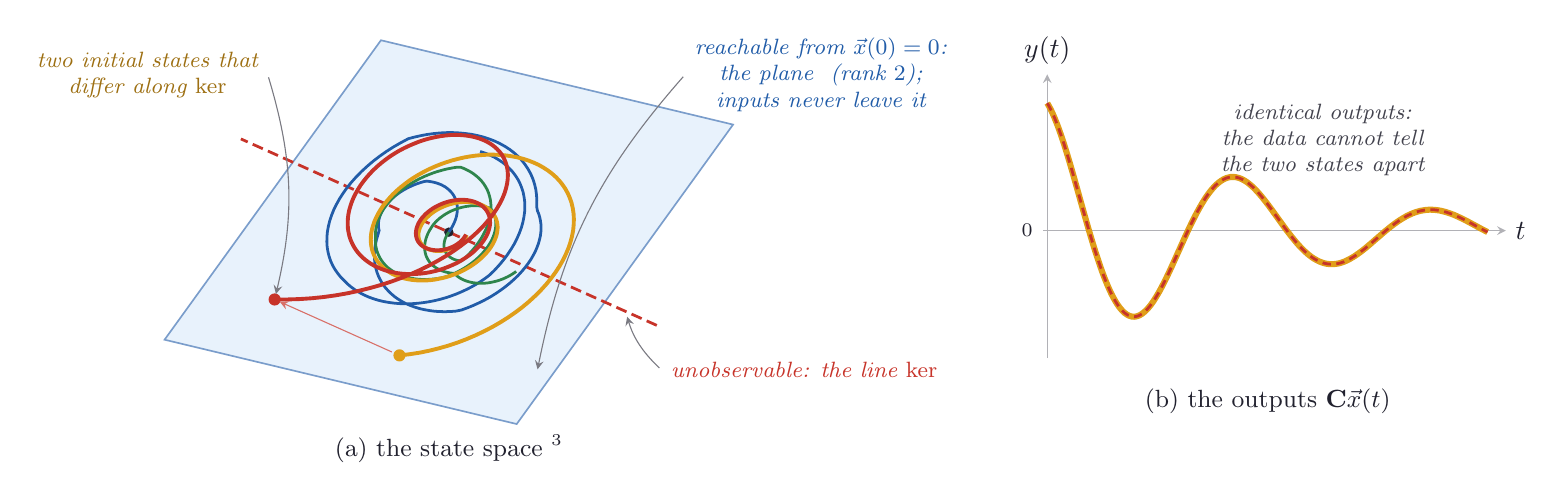
\begin{tikzpicture}[ink/.style={line width=0.9pt, ndInk}, faint/.style={line width=0.4pt, ndInk!35}, dashedink/.style={line width=0.5pt, ndInk!55, dash pattern=on 2.5pt off 2pt}, vec/.style={->, >=stealth, line width=1.2pt}, note/.style={font=\footnotesize\itshape, text=ndInk!85, align=center}, pointer/.style={->, >=stealth, line width=0.4pt, ndInk!60, shorten >=2pt, shorten <=1pt}, dot/.style={circle, fill=ndInk, inner sep=0pt, minimum size=3.4pt}, wash/.style={fill=ndSky, fill opacity=0.55}, every node/.style={text=ndInk}]
\definecolor{ndInk}{rgb}{0.13,0.13,0.18}
\definecolor{ndPaper}{rgb}{0.99,0.96,0.88}
\definecolor{ndSky}{rgb}{0.84,0.91,0.98}
\definecolor{ndRose}{rgb}{0.98,0.86,0.84}
\definecolor{ndBlue}{rgb}{0.13,0.36,0.66}
\definecolor{ndRed}{rgb}{0.78,0.20,0.16}
\definecolor{ndGold}{rgb}{0.88,0.62,0.10}
\definecolor{ndGreen}{rgb}{0.18,0.52,0.30}
\filldraw[fill=ndSky, fill opacity=0.55, draw=ndBlue!60, line width=0.6pt] (-0.862,2.437) -- (-3.610,-1.366) -- (0.862,-2.437) -- (3.610,1.366) -- cycle;
\draw[line width=1.0pt, ndRed, dash pattern=on 4pt off 2pt] (2.641,-1.184) -- (-2.641,1.184);
\node[dot] at (0.000,0.000) {};
\draw[line width=1.0pt, ndBlue] (0.000,0.000) -- (0.022,0.033) -- (0.042,0.066) -- (0.059,0.099) -- (0.074,0.132) -- (0.086,0.164) -- (0.096,0.197) -- (0.102,0.228) -- (0.107,0.260) -- (0.108,0.290) -- (0.108,0.320) -- (0.104,0.349) -- (0.099,0.377) -- (0.091,0.404) -- (0.080,0.430) -- (0.068,0.455) -- (0.054,0.478) -- (0.037,0.500) -- (0.018,0.521) -- (-0.002,0.540) -- (-0.024,0.558) -- (-0.047,0.575) -- (-0.072,0.589) -- (-0.099,0.603) -- (-0.127,0.614) -- (-0.155,0.624) -- (-0.185,0.632) -- (-0.216,0.639) -- (-0.247,0.644) -- (-0.279,0.648) -- (-0.317,0.642) -- (-0.358,0.630) -- (-0.397,0.617) -- (-0.436,0.603) -- (-0.474,0.586) -- (-0.511,0.569) -- (-0.547,0.550) -- (-0.581,0.531) -- (-0.614,0.510) -- (-0.645,0.488) -- (-0.675,0.466) -- (-0.703,0.442) -- (-0.730,0.418) -- (-0.754,0.394) -- (-0.777,0.368) -- (-0.798,0.343) -- (-0.816,0.317) -- (-0.833,0.291) -- (-0.848,0.266) -- (-0.861,0.240) -- (-0.872,0.214) -- (-0.880,0.188) -- (-0.887,0.163) -- (-0.891,0.138) -- (-0.894,0.114) -- (-0.895,0.090) -- (-0.893,0.067) -- (-0.890,0.044) -- (-0.885,0.022) -- (-0.899,-0.028) -- (-0.918,-0.093) -- (-0.932,-0.157) -- (-0.941,-0.220) -- (-0.945,-0.281) -- (-0.944,-0.342) -- (-0.938,-0.400) -- (-0.928,-0.456) -- (-0.912,-0.511) -- (-0.892,-0.563) -- (-0.867,-0.613) -- (-0.839,-0.660) -- (-0.806,-0.705) -- (-0.769,-0.746) -- (-0.729,-0.785) -- (-0.685,-0.822) -- (-0.638,-0.855) -- (-0.588,-0.885) -- (-0.536,-0.911) -- (-0.480,-0.935) -- (-0.423,-0.955) -- (-0.363,-0.973) -- (-0.302,-0.986) -- (-0.239,-0.997) -- (-0.175,-1.005) -- (-0.110,-1.009) -- (-0.044,-1.010) -- (0.022,-1.008) -- (0.089,-1.003) -- (0.160,-0.989) -- (0.237,-0.961) -- (0.313,-0.930) -- (0.387,-0.896) -- (0.459,-0.860) -- (0.528,-0.822) -- (0.594,-0.781) -- (0.657,-0.738) -- (0.717,-0.694) -- (0.774,-0.648) -- (0.828,-0.600) -- (0.878,-0.552) -- (0.924,-0.502) -- (0.966,-0.452) -- (1.005,-0.401) -- (1.040,-0.350) -- (1.070,-0.298) -- (1.097,-0.247) -- (1.119,-0.196) -- (1.138,-0.145) -- (1.152,-0.094) -- (1.163,-0.045) -- (1.169,0.004) -- (1.171,0.052) -- (1.170,0.098) -- (1.164,0.143) -- (1.155,0.187) -- (1.143,0.229) -- (1.126,0.269) -- (1.116,0.321) -- (1.118,0.396) -- (1.114,0.469) -- (1.105,0.540) -- (1.089,0.609) -- (1.068,0.675) -- (1.041,0.738) -- (1.008,0.798) -- (0.971,0.855) -- (0.929,0.909) -- (0.882,0.959) -- (0.830,1.006) -- (0.775,1.049) -- (0.715,1.088) -- (0.652,1.123) -- (0.586,1.155) -- (0.517,1.182) -- (0.445,1.206) -- (0.371,1.225) -- (0.294,1.241) -- (0.216,1.252) -- (0.136,1.260) -- (0.056,1.264) -- (-0.026,1.264) -- (-0.108,1.260) -- (-0.190,1.252) -- (-0.272,1.241) -- (-0.353,1.226) -- (-0.434,1.208) -- (-0.514,1.187) -- (-0.611,1.135) -- (-0.705,1.081) -- (-0.794,1.024) -- (-0.879,0.964) -- (-0.960,0.902) -- (-1.036,0.837) -- (-1.108,0.771) -- (-1.174,0.704) -- (-1.236,0.635) -- (-1.292,0.566) -- (-1.342,0.495) -- (-1.388,0.424) -- (-1.427,0.353) -- (-1.462,0.283) -- (-1.490,0.212) -- (-1.513,0.142) -- (-1.530,0.073) -- (-1.542,0.006) -- (-1.548,-0.061) -- (-1.549,-0.126) -- (-1.545,-0.189) -- (-1.535,-0.250) -- (-1.520,-0.310) -- (-1.501,-0.366) -- (-1.476,-0.421) -- (-1.447,-0.472) -- (-1.413,-0.521) -- (-1.376,-0.567) -- (-1.334,-0.610) -- (-1.291,-0.654) -- (-1.244,-0.694) -- (-1.193,-0.731) -- (-1.139,-0.765) -- (-1.082,-0.795) -- (-1.023,-0.822) -- (-0.960,-0.845) -- (-0.896,-0.865) -- (-0.829,-0.881) -- (-0.761,-0.893) -- (-0.691,-0.902) -- (-0.620,-0.908) -- (-0.548,-0.910) -- (-0.476,-0.909) -- (-0.403,-0.904) -- (-0.330,-0.896) -- (-0.257,-0.885) -- (-0.185,-0.871) -- (-0.114,-0.854) -- (-0.043,-0.834) -- (0.026,-0.811) -- (0.094,-0.786) -- (0.160,-0.758) -- (0.225,-0.728) -- (0.287,-0.696) -- (0.347,-0.662) -- (0.405,-0.626) -- (0.460,-0.588) -- (0.512,-0.549) -- (0.573,-0.491) -- (0.635,-0.424) -- (0.692,-0.356) -- (0.744,-0.287) -- (0.790,-0.218) -- (0.832,-0.148) -- (0.867,-0.078) -- (0.897,-0.009) -- (0.922,0.060) -- (0.941,0.128) -- (0.954,0.195) -- (0.963,0.261) -- (0.965,0.326) -- (0.963,0.389) -- (0.955,0.450) -- (0.943,0.509) -- (0.925,0.565) -- (0.903,0.620) -- (0.876,0.672) -- (0.844,0.721) -- (0.809,0.767) -- (0.769,0.810) -- (0.726,0.851) -- (0.679,0.888) -- (0.628,0.922) -- (0.575,0.953) -- (0.518,0.980) -- (0.460,1.004) -- (0.398,1.025);
\draw[line width=1.0pt, ndGreen] (0.000,0.000) -- (-0.013,-0.019) -- (-0.024,-0.037) -- (-0.034,-0.056) -- (-0.042,-0.075) -- (-0.049,-0.093) -- (-0.054,-0.111) -- (-0.058,-0.129) -- (-0.060,-0.147) -- (-0.061,-0.164) -- (-0.061,-0.181) -- (-0.059,-0.198) -- (-0.056,-0.214) -- (-0.051,-0.229) -- (-0.046,-0.243) -- (-0.039,-0.257) -- (-0.030,-0.271) -- (-0.021,-0.283) -- (-0.010,-0.295) -- (0.001,-0.306) -- (0.013,-0.316) -- (0.027,-0.325) -- (0.041,-0.334) -- (0.056,-0.341) -- (0.072,-0.348) -- (0.088,-0.353) -- (0.105,-0.358) -- (0.122,-0.362) -- (0.140,-0.365) -- (0.158,-0.367) -- (0.199,-0.335) -- (0.249,-0.286) -- (0.295,-0.236) -- (0.337,-0.185) -- (0.375,-0.134) -- (0.409,-0.082) -- (0.439,-0.030) -- (0.465,0.022) -- (0.487,0.073) -- (0.505,0.125) -- (0.519,0.175) -- (0.528,0.225) -- (0.534,0.274) -- (0.536,0.322) -- (0.533,0.369) -- (0.527,0.414) -- (0.517,0.457) -- (0.504,0.499) -- (0.487,0.540) -- (0.466,0.578) -- (0.443,0.614) -- (0.416,0.649) -- (0.386,0.681) -- (0.353,0.710) -- (0.318,0.738) -- (0.280,0.763) -- (0.240,0.785) -- (0.198,0.806) -- (0.154,0.823) -- (0.098,0.824) -- (0.037,0.814) -- (-0.024,0.802) -- (-0.084,0.787) -- (-0.143,0.770) -- (-0.201,0.751) -- (-0.258,0.729) -- (-0.314,0.706) -- (-0.368,0.680) -- (-0.420,0.653) -- (-0.470,0.624) -- (-0.519,0.594) -- (-0.565,0.562) -- (-0.608,0.529) -- (-0.650,0.494) -- (-0.688,0.459) -- (-0.724,0.423) -- (-0.758,0.386) -- (-0.788,0.349) -- (-0.816,0.312) -- (-0.841,0.274) -- (-0.862,0.236) -- (-0.881,0.198) -- (-0.897,0.160) -- (-0.909,0.122) -- (-0.919,0.085) -- (-0.926,0.049) -- (-0.930,0.013) -- (-0.931,-0.022) -- (-0.931,-0.059) -- (-0.933,-0.102) -- (-0.931,-0.144) -- (-0.926,-0.185) -- (-0.917,-0.224) -- (-0.905,-0.262) -- (-0.890,-0.298) -- (-0.872,-0.332) -- (-0.851,-0.365) -- (-0.827,-0.396) -- (-0.801,-0.425) -- (-0.772,-0.452) -- (-0.740,-0.476) -- (-0.707,-0.499) -- (-0.671,-0.519) -- (-0.633,-0.537) -- (-0.594,-0.553) -- (-0.553,-0.567) -- (-0.511,-0.578) -- (-0.467,-0.587) -- (-0.423,-0.594) -- (-0.377,-0.599) -- (-0.332,-0.601) -- (-0.285,-0.601) -- (-0.238,-0.599) -- (-0.192,-0.595) -- (-0.145,-0.589) -- (-0.098,-0.581) -- (-0.052,-0.571) -- (-0.005,-0.556) -- (0.045,-0.536) -- (0.093,-0.513) -- (0.139,-0.489) -- (0.184,-0.464) -- (0.227,-0.437) -- (0.268,-0.409) -- (0.307,-0.380) -- (0.344,-0.350) -- (0.378,-0.318) -- (0.410,-0.287) -- (0.440,-0.254) -- (0.467,-0.221) -- (0.492,-0.188) -- (0.514,-0.154) -- (0.534,-0.121) -- (0.551,-0.087) -- (0.565,-0.053) -- (0.577,-0.020) -- (0.586,0.013) -- (0.592,0.045) -- (0.596,0.077) -- (0.597,0.108) -- (0.595,0.138) -- (0.591,0.167) -- (0.585,0.196) -- (0.576,0.223) -- (0.565,0.249) -- (0.552,0.274) -- (0.536,0.298) -- (0.511,0.307) -- (0.484,0.316) -- (0.456,0.323) -- (0.428,0.328) -- (0.399,0.332) -- (0.369,0.335) -- (0.339,0.336) -- (0.309,0.335) -- (0.279,0.334) -- (0.248,0.330) -- (0.218,0.326) -- (0.188,0.320) -- (0.158,0.313) -- (0.129,0.305) -- (0.100,0.296) -- (0.071,0.285) -- (0.044,0.274) -- (0.017,0.262) -- (-0.009,0.248) -- (-0.034,0.234) -- (-0.058,0.219) -- (-0.081,0.203) -- (-0.103,0.187) -- (-0.124,0.170) -- (-0.143,0.153) -- (-0.162,0.135) -- (-0.178,0.117) -- (-0.194,0.099) -- (-0.208,0.080) -- (-0.228,0.049) -- (-0.247,0.019) -- (-0.263,-0.012) -- (-0.276,-0.043) -- (-0.287,-0.073) -- (-0.296,-0.104) -- (-0.302,-0.133) -- (-0.306,-0.163) -- (-0.307,-0.191) -- (-0.306,-0.219) -- (-0.303,-0.246) -- (-0.297,-0.272) -- (-0.290,-0.297) -- (-0.280,-0.321) -- (-0.268,-0.344) -- (-0.254,-0.366) -- (-0.239,-0.387) -- (-0.221,-0.406) -- (-0.202,-0.424) -- (-0.181,-0.440) -- (-0.159,-0.455) -- (-0.135,-0.469) -- (-0.111,-0.481) -- (-0.085,-0.492) -- (-0.058,-0.501) -- (-0.030,-0.509) -- (-0.001,-0.515) -- (0.028,-0.520) -- (0.058,-0.523) -- (0.081,-0.536) -- (0.101,-0.554) -- (0.122,-0.570) -- (0.145,-0.585) -- (0.169,-0.598) -- (0.195,-0.610) -- (0.221,-0.620) -- (0.249,-0.629) -- (0.277,-0.636) -- (0.307,-0.642) -- (0.337,-0.646) -- (0.367,-0.649) -- (0.398,-0.650) -- (0.429,-0.649) -- (0.460,-0.648) -- (0.492,-0.645) -- (0.523,-0.640) -- (0.554,-0.634) -- (0.585,-0.627) -- (0.615,-0.619) -- (0.645,-0.609) -- (0.674,-0.599) -- (0.703,-0.587) -- (0.731,-0.574) -- (0.758,-0.561) -- (0.784,-0.546) -- (0.809,-0.531) -- (0.833,-0.515) -- (0.855,-0.498);
\draw[line width=1.4pt, ndGold] (-0.627,-1.565) -- (-0.502,-1.551) -- (-0.378,-1.532) -- (-0.255,-1.507) -- (-0.132,-1.477) -- (-0.012,-1.443) -- (0.106,-1.404) -- (0.222,-1.360) -- (0.335,-1.312) -- (0.445,-1.260) -- (0.551,-1.205) -- (0.653,-1.146) -- (0.751,-1.084) -- (0.845,-1.019) -- (0.934,-0.952) -- (1.018,-0.882) -- (1.096,-0.810) -- (1.169,-0.737) -- (1.237,-0.662) -- (1.299,-0.586) -- (1.355,-0.510) -- (1.405,-0.433) -- (1.449,-0.356) -- (1.487,-0.278) -- (1.519,-0.202) -- (1.545,-0.125) -- (1.565,-0.050) -- (1.579,0.024) -- (1.586,0.097) -- (1.588,0.168) -- (1.584,0.237) -- (1.574,0.304) -- (1.559,0.369) -- (1.538,0.431) -- (1.512,0.491) -- (1.481,0.548) -- (1.445,0.601) -- (1.405,0.652) -- (1.360,0.699) -- (1.311,0.743) -- (1.258,0.783) -- (1.201,0.820) -- (1.141,0.854) -- (1.078,0.883) -- (1.012,0.909) -- (0.944,0.931) -- (0.873,0.949) -- (0.801,0.963) -- (0.726,0.974) -- (0.651,0.981) -- (0.574,0.984) -- (0.497,0.984) -- (0.419,0.979) -- (0.342,0.972) -- (0.264,0.961) -- (0.187,0.947) -- (0.110,0.929) -- (0.034,0.909) -- (-0.040,0.885) -- (-0.113,0.859) -- (-0.184,0.830) -- (-0.253,0.799) -- (-0.320,0.765) -- (-0.385,0.729) -- (-0.447,0.691) -- (-0.507,0.651) -- (-0.563,0.609) -- (-0.617,0.566) -- (-0.667,0.522) -- (-0.714,0.477) -- (-0.757,0.430) -- (-0.797,0.383) -- (-0.834,0.336) -- (-0.866,0.288) -- (-0.895,0.239) -- (-0.920,0.191) -- (-0.942,0.143) -- (-0.959,0.095) -- (-0.973,0.048) -- (-0.983,0.002) -- (-0.989,-0.044) -- (-0.991,-0.089) -- (-0.990,-0.133) -- (-0.985,-0.175) -- (-0.977,-0.216) -- (-0.965,-0.255) -- (-0.950,-0.293) -- (-0.932,-0.329) -- (-0.911,-0.363) -- (-0.886,-0.396) -- (-0.859,-0.426) -- (-0.830,-0.454) -- (-0.797,-0.480) -- (-0.763,-0.504) -- (-0.726,-0.526) -- (-0.687,-0.545) -- (-0.647,-0.562) -- (-0.605,-0.576) -- (-0.561,-0.589) -- (-0.516,-0.598) -- (-0.470,-0.606) -- (-0.423,-0.611) -- (-0.376,-0.614) -- (-0.328,-0.614) -- (-0.279,-0.613) -- (-0.231,-0.609) -- (-0.182,-0.603) -- (-0.134,-0.594) -- (-0.086,-0.584) -- (-0.038,-0.572) -- (0.008,-0.558) -- (0.054,-0.542) -- (0.099,-0.525) -- (0.143,-0.506) -- (0.185,-0.485) -- (0.226,-0.463) -- (0.265,-0.440) -- (0.303,-0.415) -- (0.339,-0.390) -- (0.373,-0.363) -- (0.405,-0.336) -- (0.435,-0.308) -- (0.463,-0.279) -- (0.489,-0.250) -- (0.513,-0.220) -- (0.534,-0.190) -- (0.553,-0.160) -- (0.569,-0.130) -- (0.583,-0.100) -- (0.595,-0.070) -- (0.605,-0.041) -- (0.612,-0.011) -- (0.616,0.017) -- (0.619,0.046) -- (0.619,0.073) -- (0.616,0.100) -- (0.612,0.126) -- (0.605,0.151) -- (0.597,0.175) -- (0.586,0.198) -- (0.573,0.219) -- (0.559,0.240) -- (0.543,0.259) -- (0.525,0.277) -- (0.505,0.294) -- (0.484,0.309) -- (0.462,0.323) -- (0.438,0.336) -- (0.413,0.347) -- (0.387,0.357) -- (0.360,0.365) -- (0.332,0.371) -- (0.304,0.377) -- (0.275,0.380) -- (0.245,0.383) -- (0.215,0.384) -- (0.185,0.383) -- (0.155,0.381) -- (0.125,0.378) -- (0.094,0.373) -- (0.064,0.367) -- (0.035,0.360) -- (0.005,0.352) -- (-0.024,0.342) -- (-0.052,0.332) -- (-0.079,0.320) -- (-0.106,0.308) -- (-0.132,0.294) -- (-0.157,0.280) -- (-0.181,0.265) -- (-0.204,0.249) -- (-0.225,0.233) -- (-0.246,0.216) -- (-0.265,0.198) -- (-0.283,0.181) -- (-0.300,0.163) -- (-0.315,0.144) -- (-0.329,0.126) -- (-0.341,0.107) -- (-0.352,0.088) -- (-0.361,0.069) -- (-0.369,0.051) -- (-0.375,0.032) -- (-0.380,0.014) -- (-0.384,-0.004) -- (-0.386,-0.022) -- (-0.386,-0.039) -- (-0.385,-0.056) -- (-0.383,-0.073) -- (-0.380,-0.088) -- (-0.375,-0.104) -- (-0.368,-0.118) -- (-0.361,-0.132) -- (-0.352,-0.145) -- (-0.343,-0.158) -- (-0.332,-0.169) -- (-0.320,-0.180) -- (-0.307,-0.190) -- (-0.293,-0.199) -- (-0.279,-0.207) -- (-0.263,-0.214) -- (-0.247,-0.221) -- (-0.231,-0.226) -- (-0.214,-0.230) -- (-0.196,-0.234) -- (-0.178,-0.237) -- (-0.160,-0.238) -- (-0.141,-0.239) -- (-0.122,-0.239) -- (-0.104,-0.238) -- (-0.085,-0.237) -- (-0.066,-0.234) -- (-0.047,-0.231) -- (-0.028,-0.226) -- (-0.010,-0.221) -- (0.008,-0.216) -- (0.026,-0.209) -- (0.043,-0.202) -- (0.060,-0.195) -- (0.077,-0.187) -- (0.092,-0.178) -- (0.108,-0.169) -- (0.122,-0.159) -- (0.136,-0.149) -- (0.149,-0.139) -- (0.161,-0.128) -- (0.173,-0.117) -- (0.183,-0.106) -- (0.193,-0.094) -- (0.202,-0.083) -- (0.210,-0.071) -- (0.217,-0.059) -- (0.223,-0.047) -- (0.229,-0.036);
\draw[line width=1.4pt, ndRed] (-2.212,-0.855) -- (-2.054,-0.855) -- (-1.898,-0.850) -- (-1.743,-0.840) -- (-1.590,-0.824) -- (-1.439,-0.803) -- (-1.291,-0.777) -- (-1.146,-0.746) -- (-1.005,-0.711) -- (-0.867,-0.672) -- (-0.734,-0.629) -- (-0.605,-0.582) -- (-0.480,-0.532) -- (-0.361,-0.478) -- (-0.247,-0.422) -- (-0.139,-0.363) -- (-0.036,-0.302) -- (0.060,-0.240) -- (0.151,-0.175) -- (0.236,-0.110) -- (0.314,-0.043) -- (0.386,0.024) -- (0.451,0.092) -- (0.510,0.160) -- (0.562,0.228) -- (0.608,0.295) -- (0.647,0.362) -- (0.680,0.427) -- (0.706,0.491) -- (0.726,0.554) -- (0.740,0.616) -- (0.748,0.675) -- (0.750,0.732) -- (0.746,0.787) -- (0.736,0.839) -- (0.721,0.888) -- (0.701,0.935) -- (0.676,0.979) -- (0.646,1.019) -- (0.612,1.056) -- (0.574,1.090) -- (0.531,1.121) -- (0.485,1.148) -- (0.436,1.171) -- (0.383,1.191) -- (0.328,1.207) -- (0.270,1.219) -- (0.210,1.228) -- (0.148,1.233) -- (0.085,1.235) -- (0.020,1.233) -- (-0.046,1.227) -- (-0.112,1.218) -- (-0.179,1.205) -- (-0.246,1.190) -- (-0.313,1.171) -- (-0.379,1.149) -- (-0.444,1.123) -- (-0.509,1.095) -- (-0.572,1.065) -- (-0.634,1.032) -- (-0.694,0.996) -- (-0.752,0.958) -- (-0.807,0.918) -- (-0.861,0.876) -- (-0.912,0.832) -- (-0.960,0.787) -- (-1.005,0.740) -- (-1.047,0.692) -- (-1.086,0.643) -- (-1.122,0.594) -- (-1.154,0.543) -- (-1.183,0.492) -- (-1.209,0.441) -- (-1.230,0.390) -- (-1.248,0.338) -- (-1.263,0.287) -- (-1.274,0.236) -- (-1.281,0.186) -- (-1.284,0.137) -- (-1.284,0.088) -- (-1.281,0.041) -- (-1.273,-0.006) -- (-1.263,-0.051) -- (-1.249,-0.094) -- (-1.231,-0.136) -- (-1.211,-0.176) -- (-1.187,-0.215) -- (-1.160,-0.252) -- (-1.131,-0.286) -- (-1.099,-0.319) -- (-1.064,-0.349) -- (-1.027,-0.377) -- (-0.988,-0.403) -- (-0.946,-0.427) -- (-0.903,-0.448) -- (-0.858,-0.467) -- (-0.811,-0.484) -- (-0.763,-0.498) -- (-0.714,-0.509) -- (-0.664,-0.519) -- (-0.613,-0.526) -- (-0.562,-0.530) -- (-0.510,-0.533) -- (-0.458,-0.533) -- (-0.405,-0.530) -- (-0.353,-0.526) -- (-0.301,-0.519) -- (-0.250,-0.511) -- (-0.199,-0.500) -- (-0.149,-0.488) -- (-0.100,-0.473) -- (-0.052,-0.457) -- (-0.005,-0.439) -- (0.040,-0.420) -- (0.084,-0.400) -- (0.127,-0.378) -- (0.167,-0.354) -- (0.206,-0.330) -- (0.243,-0.305) -- (0.278,-0.279) -- (0.311,-0.252) -- (0.341,-0.224) -- (0.369,-0.196) -- (0.395,-0.168) -- (0.419,-0.139) -- (0.440,-0.110) -- (0.459,-0.081) -- (0.476,-0.052) -- (0.490,-0.023) -- (0.501,0.006) -- (0.510,0.034) -- (0.517,0.062) -- (0.522,0.089) -- (0.524,0.116) -- (0.523,0.142) -- (0.521,0.167) -- (0.516,0.191) -- (0.509,0.214) -- (0.500,0.236) -- (0.490,0.257) -- (0.477,0.277) -- (0.462,0.295) -- (0.446,0.313) -- (0.428,0.329) -- (0.409,0.343) -- (0.388,0.357) -- (0.366,0.368) -- (0.342,0.379) -- (0.318,0.388) -- (0.292,0.395) -- (0.266,0.401) -- (0.239,0.406) -- (0.211,0.409) -- (0.183,0.411) -- (0.154,0.411) -- (0.125,0.410) -- (0.096,0.407) -- (0.067,0.403) -- (0.038,0.398) -- (0.009,0.392) -- (-0.019,0.384) -- (-0.048,0.375) -- (-0.075,0.365) -- (-0.102,0.354) -- (-0.129,0.342) -- (-0.155,0.329) -- (-0.180,0.315) -- (-0.204,0.301) -- (-0.226,0.285) -- (-0.248,0.269) -- (-0.269,0.252) -- (-0.289,0.235) -- (-0.307,0.217) -- (-0.324,0.199) -- (-0.340,0.181) -- (-0.354,0.162) -- (-0.367,0.143) -- (-0.379,0.124) -- (-0.389,0.105) -- (-0.397,0.085) -- (-0.404,0.066) -- (-0.410,0.048) -- (-0.414,0.029) -- (-0.417,0.010) -- (-0.418,-0.008) -- (-0.418,-0.025) -- (-0.417,-0.042) -- (-0.414,-0.059) -- (-0.409,-0.075) -- (-0.404,-0.091) -- (-0.397,-0.105) -- (-0.389,-0.120) -- (-0.380,-0.133) -- (-0.369,-0.146) -- (-0.358,-0.157) -- (-0.346,-0.168) -- (-0.332,-0.178) -- (-0.318,-0.188) -- (-0.303,-0.196) -- (-0.287,-0.204) -- (-0.271,-0.210) -- (-0.254,-0.216) -- (-0.236,-0.220) -- (-0.218,-0.224) -- (-0.200,-0.227) -- (-0.181,-0.229) -- (-0.162,-0.230) -- (-0.143,-0.230) -- (-0.123,-0.230) -- (-0.104,-0.228) -- (-0.085,-0.226) -- (-0.065,-0.222) -- (-0.046,-0.218) -- (-0.028,-0.214) -- (-0.009,-0.208) -- (0.009,-0.202) -- (0.027,-0.195) -- (0.044,-0.188) -- (0.061,-0.180) -- (0.077,-0.171) -- (0.092,-0.162) -- (0.107,-0.152) -- (0.121,-0.142) -- (0.135,-0.132) -- (0.147,-0.122) -- (0.159,-0.111) -- (0.170,-0.100) -- (0.180,-0.088) -- (0.189,-0.077) -- (0.197,-0.065) -- (0.205,-0.054) -- (0.211,-0.042) -- (0.217,-0.030);
\node[dot, fill=ndGold, minimum size=4.4pt] at (-0.627,-1.565) {};
\node[dot, fill=ndRed, minimum size=4.4pt] at (-2.212,-0.855) {};
\draw[pointer, ndRed!70, shorten <=3pt] (-0.627,-1.565) -- (-2.212,-0.855);
\node[note, anchor=west, text=ndBlue] (pl) at (3.0,2.0) {reachable from $\vec x(0)=0$:\\ the plane $\ran\CM$ (rank $2$);\\ inputs never leave it};
\draw[pointer] (pl.west) to[bend right=15] (1.113,-1.811);
\node[note, anchor=west, text=ndRed] (ln) at (2.7,-1.75) {unobservable: the line $\ker\OM$};
\draw[pointer] (ln.west) to[bend left=15] (2.245,-1.007);
\node[note, anchor=east, text=ndGold!70!black] (st) at (-2.3,2.0) {two initial states that\\ differ along $\ker\OM$};
\draw[pointer] (st.east) to[bend left=15] (-2.212,-0.855);
\node[font=\small] at (0,-2.75) {(a) the state space $\R^3$};
\draw[faint, ->, >=stealth] (7.600,0.019) -- (13.424,0.019) node[right, text=ndInk] {$t$};
\draw[faint, ->, >=stealth] (7.600,-1.600) -- (7.600,2.004) node[above, text=ndInk] {$y(t)$};
\draw[faint] (7.660,0.019) -- (7.540,0.019) node[left, font=\scriptsize, text=ndInk] {$0$};
\draw[line width=2.2pt, ndGold] (7.600,1.638) -- (7.624,1.597) -- (7.648,1.550) -- (7.672,1.499) -- (7.696,1.443) -- (7.720,1.383) -- (7.744,1.320) -- (7.768,1.252) -- (7.792,1.181) -- (7.816,1.108) -- (7.840,1.031) -- (7.864,0.953) -- (7.888,0.872) -- (7.912,0.790) -- (7.936,0.706) -- (7.960,0.621) -- (7.984,0.536) -- (8.008,0.450) -- (8.032,0.364) -- (8.056,0.279) -- (8.080,0.194) -- (8.104,0.110) -- (8.128,0.027) -- (8.152,-0.054) -- (8.176,-0.134) -- (8.200,-0.212) -- (8.224,-0.287) -- (8.248,-0.360) -- (8.272,-0.431) -- (8.296,-0.498) -- (8.320,-0.563) -- (8.344,-0.624) -- (8.368,-0.681) -- (8.392,-0.736) -- (8.416,-0.786) -- (8.440,-0.832) -- (8.464,-0.875) -- (8.488,-0.914) -- (8.512,-0.948) -- (8.536,-0.978) -- (8.560,-1.005) -- (8.584,-1.027) -- (8.608,-1.044) -- (8.632,-1.058) -- (8.656,-1.067) -- (8.680,-1.073) -- (8.704,-1.074) -- (8.728,-1.071) -- (8.752,-1.064) -- (8.776,-1.054) -- (8.800,-1.039) -- (8.824,-1.021) -- (8.848,-1.000) -- (8.872,-0.975) -- (8.896,-0.948) -- (8.920,-0.917) -- (8.944,-0.883) -- (8.968,-0.846) -- (8.992,-0.807) -- (9.016,-0.766) -- (9.040,-0.723) -- (9.064,-0.677) -- (9.088,-0.630) -- (9.112,-0.582) -- (9.136,-0.532) -- (9.160,-0.481) -- (9.184,-0.429) -- (9.208,-0.376) -- (9.232,-0.323) -- (9.256,-0.269) -- (9.280,-0.216) -- (9.304,-0.162) -- (9.328,-0.109) -- (9.352,-0.056) -- (9.376,-0.004) -- (9.400,0.047) -- (9.424,0.097) -- (9.448,0.146) -- (9.472,0.194) -- (9.496,0.240) -- (9.520,0.284) -- (9.544,0.327) -- (9.568,0.368) -- (9.592,0.407) -- (9.616,0.444) -- (9.640,0.478) -- (9.664,0.510) -- (9.688,0.540) -- (9.712,0.568) -- (9.736,0.593) -- (9.760,0.615) -- (9.784,0.635) -- (9.808,0.652) -- (9.832,0.667) -- (9.856,0.679) -- (9.880,0.689) -- (9.904,0.695) -- (9.928,0.700) -- (9.952,0.701) -- (9.976,0.700) -- (10.000,0.697) -- (10.024,0.691) -- (10.048,0.683) -- (10.072,0.673) -- (10.096,0.660) -- (10.120,0.646) -- (10.144,0.629) -- (10.168,0.610) -- (10.192,0.590) -- (10.216,0.568) -- (10.240,0.544) -- (10.264,0.519) -- (10.288,0.492) -- (10.312,0.464) -- (10.336,0.435) -- (10.360,0.405) -- (10.384,0.374) -- (10.408,0.343) -- (10.432,0.310) -- (10.456,0.278) -- (10.480,0.244) -- (10.504,0.211) -- (10.528,0.178) -- (10.552,0.144) -- (10.576,0.111) -- (10.600,0.078) -- (10.624,0.045) -- (10.648,0.013) -- (10.672,-0.018) -- (10.696,-0.049) -- (10.720,-0.079) -- (10.744,-0.108) -- (10.768,-0.137) -- (10.792,-0.164) -- (10.816,-0.190) -- (10.840,-0.214) -- (10.864,-0.238) -- (10.888,-0.260) -- (10.912,-0.281) -- (10.936,-0.300) -- (10.960,-0.318) -- (10.984,-0.334) -- (11.008,-0.348) -- (11.032,-0.361) -- (11.056,-0.373) -- (11.080,-0.382) -- (11.104,-0.391) -- (11.128,-0.397) -- (11.152,-0.402) -- (11.176,-0.405) -- (11.200,-0.407) -- (11.224,-0.407) -- (11.248,-0.405) -- (11.272,-0.402) -- (11.296,-0.398) -- (11.320,-0.392) -- (11.344,-0.384) -- (11.368,-0.376) -- (11.392,-0.366) -- (11.416,-0.354) -- (11.440,-0.342) -- (11.464,-0.328) -- (11.488,-0.314) -- (11.512,-0.299) -- (11.536,-0.282) -- (11.560,-0.265) -- (11.584,-0.247) -- (11.608,-0.229) -- (11.632,-0.210) -- (11.656,-0.190) -- (11.680,-0.170) -- (11.704,-0.150) -- (11.728,-0.129) -- (11.752,-0.108) -- (11.776,-0.087) -- (11.800,-0.067) -- (11.824,-0.046) -- (11.848,-0.025) -- (11.872,-0.005) -- (11.896,0.016) -- (11.920,0.035) -- (11.944,0.055) -- (11.968,0.074) -- (11.992,0.092) -- (12.016,0.110) -- (12.040,0.127) -- (12.064,0.144) -- (12.088,0.159) -- (12.112,0.174) -- (12.136,0.188) -- (12.160,0.202) -- (12.184,0.214) -- (12.208,0.225) -- (12.232,0.236) -- (12.256,0.245) -- (12.280,0.254) -- (12.304,0.261) -- (12.328,0.268) -- (12.352,0.273) -- (12.376,0.277) -- (12.400,0.281) -- (12.424,0.283) -- (12.448,0.285) -- (12.472,0.285) -- (12.496,0.284) -- (12.520,0.283) -- (12.544,0.280) -- (12.568,0.277) -- (12.592,0.273) -- (12.616,0.267) -- (12.640,0.261) -- (12.664,0.255) -- (12.688,0.247) -- (12.712,0.239) -- (12.736,0.230) -- (12.760,0.221) -- (12.784,0.211) -- (12.808,0.200) -- (12.832,0.189) -- (12.856,0.178) -- (12.880,0.166) -- (12.904,0.154) -- (12.928,0.142) -- (12.952,0.129) -- (12.976,0.116) -- (13.000,0.103) -- (13.024,0.090) -- (13.048,0.077) -- (13.072,0.064) -- (13.096,0.051) -- (13.120,0.038) -- (13.144,0.026) -- (13.168,0.013) -- (13.192,0.001);
\draw[line width=1.0pt, ndRed, dash pattern=on 3pt off 2pt] (7.600,1.638) -- (7.624,1.597) -- (7.648,1.550) -- (7.672,1.499) -- (7.696,1.443) -- (7.720,1.383) -- (7.744,1.320) -- (7.768,1.252) -- (7.792,1.181) -- (7.816,1.108) -- (7.840,1.031) -- (7.864,0.953) -- (7.888,0.872) -- (7.912,0.790) -- (7.936,0.706) -- (7.960,0.621) -- (7.984,0.536) -- (8.008,0.450) -- (8.032,0.364) -- (8.056,0.279) -- (8.080,0.194) -- (8.104,0.110) -- (8.128,0.027) -- (8.152,-0.054) -- (8.176,-0.134) -- (8.200,-0.212) -- (8.224,-0.287) -- (8.248,-0.360) -- (8.272,-0.431) -- (8.296,-0.498) -- (8.320,-0.563) -- (8.344,-0.624) -- (8.368,-0.681) -- (8.392,-0.736) -- (8.416,-0.786) -- (8.440,-0.832) -- (8.464,-0.875) -- (8.488,-0.914) -- (8.512,-0.948) -- (8.536,-0.978) -- (8.560,-1.005) -- (8.584,-1.027) -- (8.608,-1.044) -- (8.632,-1.058) -- (8.656,-1.067) -- (8.680,-1.073) -- (8.704,-1.074) -- (8.728,-1.071) -- (8.752,-1.064) -- (8.776,-1.054) -- (8.800,-1.039) -- (8.824,-1.021) -- (8.848,-1.000) -- (8.872,-0.975) -- (8.896,-0.948) -- (8.920,-0.917) -- (8.944,-0.883) -- (8.968,-0.846) -- (8.992,-0.807) -- (9.016,-0.766) -- (9.040,-0.723) -- (9.064,-0.677) -- (9.088,-0.630) -- (9.112,-0.582) -- (9.136,-0.532) -- (9.160,-0.481) -- (9.184,-0.429) -- (9.208,-0.376) -- (9.232,-0.323) -- (9.256,-0.269) -- (9.280,-0.216) -- (9.304,-0.162) -- (9.328,-0.109) -- (9.352,-0.056) -- (9.376,-0.004) -- (9.400,0.047) -- (9.424,0.097) -- (9.448,0.146) -- (9.472,0.194) -- (9.496,0.240) -- (9.520,0.284) -- (9.544,0.327) -- (9.568,0.368) -- (9.592,0.407) -- (9.616,0.444) -- (9.640,0.478) -- (9.664,0.510) -- (9.688,0.540) -- (9.712,0.568) -- (9.736,0.593) -- (9.760,0.615) -- (9.784,0.635) -- (9.808,0.652) -- (9.832,0.667) -- (9.856,0.679) -- (9.880,0.689) -- (9.904,0.695) -- (9.928,0.700) -- (9.952,0.701) -- (9.976,0.700) -- (10.000,0.697) -- (10.024,0.691) -- (10.048,0.683) -- (10.072,0.673) -- (10.096,0.660) -- (10.120,0.646) -- (10.144,0.629) -- (10.168,0.610) -- (10.192,0.590) -- (10.216,0.568) -- (10.240,0.544) -- (10.264,0.519) -- (10.288,0.492) -- (10.312,0.464) -- (10.336,0.435) -- (10.360,0.405) -- (10.384,0.374) -- (10.408,0.343) -- (10.432,0.310) -- (10.456,0.278) -- (10.480,0.244) -- (10.504,0.211) -- (10.528,0.178) -- (10.552,0.144) -- (10.576,0.111) -- (10.600,0.078) -- (10.624,0.045) -- (10.648,0.013) -- (10.672,-0.018) -- (10.696,-0.049) -- (10.720,-0.079) -- (10.744,-0.108) -- (10.768,-0.137) -- (10.792,-0.164) -- (10.816,-0.190) -- (10.840,-0.214) -- (10.864,-0.238) -- (10.888,-0.260) -- (10.912,-0.281) -- (10.936,-0.300) -- (10.960,-0.318) -- (10.984,-0.334) -- (11.008,-0.348) -- (11.032,-0.361) -- (11.056,-0.373) -- (11.080,-0.382) -- (11.104,-0.391) -- (11.128,-0.397) -- (11.152,-0.402) -- (11.176,-0.405) -- (11.200,-0.407) -- (11.224,-0.407) -- (11.248,-0.405) -- (11.272,-0.402) -- (11.296,-0.398) -- (11.320,-0.392) -- (11.344,-0.384) -- (11.368,-0.376) -- (11.392,-0.366) -- (11.416,-0.354) -- (11.440,-0.342) -- (11.464,-0.328) -- (11.488,-0.314) -- (11.512,-0.299) -- (11.536,-0.282) -- (11.560,-0.265) -- (11.584,-0.247) -- (11.608,-0.229) -- (11.632,-0.210) -- (11.656,-0.190) -- (11.680,-0.170) -- (11.704,-0.150) -- (11.728,-0.129) -- (11.752,-0.108) -- (11.776,-0.087) -- (11.800,-0.067) -- (11.824,-0.046) -- (11.848,-0.025) -- (11.872,-0.005) -- (11.896,0.016) -- (11.920,0.035) -- (11.944,0.055) -- (11.968,0.074) -- (11.992,0.092) -- (12.016,0.110) -- (12.040,0.127) -- (12.064,0.144) -- (12.088,0.159) -- (12.112,0.174) -- (12.136,0.188) -- (12.160,0.202) -- (12.184,0.214) -- (12.208,0.225) -- (12.232,0.236) -- (12.256,0.245) -- (12.280,0.254) -- (12.304,0.261) -- (12.328,0.268) -- (12.352,0.273) -- (12.376,0.277) -- (12.400,0.281) -- (12.424,0.283) -- (12.448,0.285) -- (12.472,0.285) -- (12.496,0.284) -- (12.520,0.283) -- (12.544,0.280) -- (12.568,0.277) -- (12.592,0.273) -- (12.616,0.267) -- (12.640,0.261) -- (12.664,0.255) -- (12.688,0.247) -- (12.712,0.239) -- (12.736,0.230) -- (12.760,0.221) -- (12.784,0.211) -- (12.808,0.200) -- (12.832,0.189) -- (12.856,0.178) -- (12.880,0.166) -- (12.904,0.154) -- (12.928,0.142) -- (12.952,0.129) -- (12.976,0.116) -- (13.000,0.103) -- (13.024,0.090) -- (13.048,0.077) -- (13.072,0.064) -- (13.096,0.051) -- (13.120,0.038) -- (13.144,0.026) -- (13.168,0.013) -- (13.192,0.001);
\node[note, anchor=south west] at (9.680,0.586) {identical outputs:\\ the data cannot tell\\ the two states apart};
\node[font=\small] at (10.400,-2.150) {(b) the outputs $\mathbf C\vec x(t)$};
\end{tikzpicture}
}\end{center}
Inputs never leave $\ran\CM$; initial states differing along $\ker\OM$ give the same data.}
\end{frame}

\section{Bilinear systems}

\begin{frame}\ft{Bilinear dynamical systems}
\ona{The second type of system naturally occurring in open quantum system identification is the bilinear dynamical system (BDS). More succinctly, the dynamics of the controlled quantum system can be written as}
\onp{Controlled open quantum systems are \alert{bilinear} (\Chap~\ref{C.Open}):}
\begin{equation}\label{eq:ch04:BDS}
\begin{aligned}
    \dot{\vec{x}}(t) &= \mathbf{A}\vec{x}(t) + \sum_{j}\mathbf{N}_{j}u_{j}(t) \vec{x}(t),\qquad
    \vec{x}(0) = \vec{b} = \mathbf{B}\vec{x}_{0},\qquad
    \vec{y}\left(t\right) =\mathbf{C}\vec{x}\left(t\right).
\end{aligned}
\end{equation}
\ona{Here, the variables are the same as in \eqref{eq:ch04:LDS} with the addition of the bilinear coupling matrices $\mathbf{N}_j \in \R^{n\times n}$. This is a BDS of type II in the language of \citet{Sontag2009}, where the initial state is fixed, $\vec x(0) = \vec b$. Here $\mathbf{B}$ encodes the state-preparation map and, as in the linear case, enters only through the initial condition, which is why the direct driving term $\mathbf{B}\vec{u}$ of the general bilinear model is absent. The presence of $\mathbf{N}_{j}$ requires us to modify the definitions of controllability and observability \citep{Isidori1973, Sontag2009}. In the case of the BDS \eqref{eq:ch04:BDS}, this is given by the criteria}
\onp{Span criteria replace the Kalman matrices \citep{Isidori1973,Sontag2009}:}
\begin{equation}\label{eq:ch04:BDS_reach_and_obs}
\begin{aligned}
\linspan\left\{ \mathbf{A}_{i_{1}}\cdots \mathbf{A}_{i_{k}}\vec{b}:\mathbf{A}_{j}\in\left\{ \mathbf{A},\mathbf{N}_1,\dots\right\} ,k\leq n-1\right\}  &=\R^{n}, \\
\linspan\left\{ (\mathbf{A}_{i_{1}}\cdots \mathbf{A}_{i_{k}})^{\top}\mathbf{C}_{r\cdot}^{\top}:\mathbf{A}_{j}\in\left\{ \mathbf{A},\mathbf{N}_1,\dots\right\} ,k\leq n-1,r \leq p \right\} &=\R^{n},
\end{aligned}
\end{equation}
\ona{respectively, where $\mathbf{C}_{r\cdot}$ denotes the $r$-th row of the observation matrix. These criteria can be interpreted as the full rank of the matrices whose columns are the listed products; we denote these matrices $\CM^{(\mathrm{bi})}$ and $\OM^{(\mathrm{bi})}$. For $\mathbf N_j=0$ they reduce to \eqref{eq:ch04:OMCM}.}
\onp{Full rank of $\CM^{(\mathrm{bi})}$, $\OM^{(\mathrm{bi})}$; for $\mathbf N_j=0$ back to Kalman.}
\end{frame}

\begin{frame}\ft{Example: a driven qubit, nothing hidden}
\ona{The simplest bilinear system in this course is a single qubit driven by one control field. Its Hamiltonian, $H(t)=-\frac\omega2\sigma_z+\frac{u(t)}2\sigma_x$, has a drift, which makes the qubit precess about the $z$-axis at the frequency $\omega$, and a control term, which rotates it about the $x$-axis at a rate set by the amplitude $u(t)$ that we choose. The state is the Bloch vector $\vec r=(x,y,z)$ of \Chap~\ref{C.Closed}, which for one qubit is the coherence vector up to a factor $\sqrt2$, and the Schr\"odinger equation becomes}
\onp{One qubit, $H(t)=-\frac\omega2\sigma_z+\frac{u(t)}2\sigma_x$; the state is the Bloch vector $\vec r=(x,y,z)$:}
\begin{equation}\label{eq:ch04:driven}
\dot{\vec r}=\big(\mathbf A+u(t)\,\mathbf N\big)\vec r,\qquad
\mathbf A=\begin{pmatrix}0&\omega&0\\-\omega&0&0\\0&0&0\end{pmatrix},\qquad
\mathbf N=\begin{pmatrix}0&0&0\\0&0&-1\\0&1&0\end{pmatrix},
\end{equation}
\ona{a bilinear system \eqref{eq:ch04:BDS} with one input, a state of dimension $n=3$, and no affine term. Both matrices are antisymmetric, because a closed system only rotates the Bloch vector: its length, the purity, never changes (Figure~\ref{fig:ch04:driven}(a)). Measuring $\sigma_x$, $\sigma_y$ and $\sigma_z$ gives $\vec y=\vec r$, so that $\mathbf C=\Id$ and nothing is hidden: the state is exactly what we can measure. The input enters multiplied by the state, and this is what makes the system bilinear rather than linear. In a linear system $\dot{\vec x}=\mathbf A\vec x+\mathbf B\vec u$, doubling the input doubles its effect on the state. Here, a resonant pulse ($\omega=0$) of area $uT$, applied to $\ket0$, leaves $\langle\sigma_z\rangle=\cos(uT)$: a pulse of area $\pi$ flips the qubit, and a pulse of twice that area brings it back (Figure~\ref{fig:ch04:driven}(b)).}
\ona{\begin{figure}[H]\centering
\resizebox{\linewidth}{!}{% Generated by code/needham.py -- do not edit by hand.
\definecolor{qocA}{rgb}{0.00,0.45,0.70}
\definecolor{qocB}{rgb}{0.90,0.60,0.00}
\definecolor{qocC}{rgb}{0.00,0.62,0.45}
\definecolor{qocD}{rgb}{0.80,0.40,0.00}
\definecolor{qocE}{rgb}{0.80,0.60,0.70}
\definecolor{qocF}{rgb}{0.35,0.70,0.90}
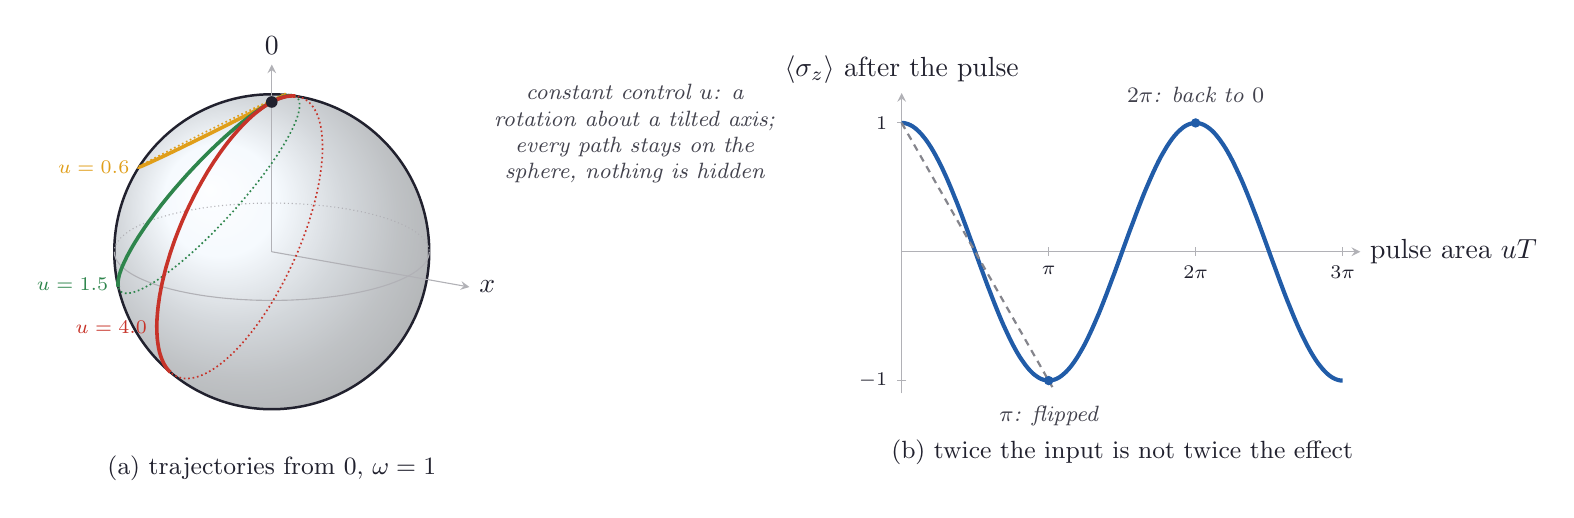
\begin{tikzpicture}[ink/.style={line width=0.9pt, ndInk}, faint/.style={line width=0.4pt, ndInk!35}, dashedink/.style={line width=0.5pt, ndInk!55, dash pattern=on 2.5pt off 2pt}, vec/.style={->, >=stealth, line width=1.2pt}, note/.style={font=\footnotesize\itshape, text=ndInk!85, align=center}, pointer/.style={->, >=stealth, line width=0.4pt, ndInk!60, shorten >=2pt, shorten <=1pt}, dot/.style={circle, fill=ndInk, inner sep=0pt, minimum size=3.4pt}, wash/.style={fill=ndSky, fill opacity=0.55}, every node/.style={text=ndInk}]
\definecolor{ndInk}{rgb}{0.13,0.13,0.18}
\definecolor{ndPaper}{rgb}{0.99,0.96,0.88}
\definecolor{ndSky}{rgb}{0.84,0.91,0.98}
\definecolor{ndRose}{rgb}{0.98,0.86,0.84}
\definecolor{ndBlue}{rgb}{0.13,0.36,0.66}
\definecolor{ndRed}{rgb}{0.78,0.20,0.16}
\definecolor{ndGold}{rgb}{0.88,0.62,0.10}
\definecolor{ndGreen}{rgb}{0.18,0.52,0.30}
\shade[ball color=ndSky!70!white, opacity=0.45] (0.000,0.000) circle (2.000);
\draw[ink] (0.000,0.000) circle (2.000);
\draw[faint] (-2.000,0.000) -- (-1.999,-0.016) -- (-1.997,-0.032) -- (-1.994,-0.048) -- (-1.989,-0.065) -- (-1.983,-0.081) -- (-1.975,-0.097) -- (-1.967,-0.113) -- (-1.956,-0.128) -- (-1.945,-0.144) -- (-1.932,-0.160) -- (-1.918,-0.176) -- (-1.902,-0.191) -- (-1.885,-0.206) -- (-1.867,-0.221) -- (-1.848,-0.237) -- (-1.827,-0.251) -- (-1.805,-0.266) -- (-1.782,-0.281) -- (-1.758,-0.295) -- (-1.732,-0.309) -- (-1.705,-0.323) -- (-1.677,-0.337) -- (-1.648,-0.350) -- (-1.618,-0.363) -- (-1.587,-0.376) -- (-1.554,-0.389) -- (-1.521,-0.401) -- (-1.486,-0.414) -- (-1.451,-0.425) -- (-1.414,-0.437) -- (-1.377,-0.448) -- (-1.338,-0.459) -- (-1.299,-0.470) -- (-1.259,-0.480) -- (-1.218,-0.490) -- (-1.176,-0.500) -- (-1.133,-0.509) -- (-1.089,-0.518) -- (-1.045,-0.527) -- (-1.000,-0.535) -- (-0.954,-0.543) -- (-0.908,-0.551) -- (-0.861,-0.558) -- (-0.813,-0.565) -- (-0.765,-0.571) -- (-0.717,-0.577) -- (-0.668,-0.583) -- (-0.618,-0.588) -- (-0.568,-0.593) -- (-0.518,-0.597) -- (-0.467,-0.601) -- (-0.416,-0.605) -- (-0.364,-0.608) -- (-0.313,-0.610) -- (-0.261,-0.613) -- (-0.209,-0.615) -- (-0.157,-0.616) -- (-0.105,-0.617) -- (-0.052,-0.618) -- (-0.000,-0.618) -- (0.052,-0.618) -- (0.105,-0.617) -- (0.157,-0.616) -- (0.209,-0.615) -- (0.261,-0.613) -- (0.313,-0.610) -- (0.364,-0.608) -- (0.416,-0.605) -- (0.467,-0.601) -- (0.518,-0.597) -- (0.568,-0.593) -- (0.618,-0.588) -- (0.668,-0.583) -- (0.717,-0.577) -- (0.765,-0.571) -- (0.813,-0.565) -- (0.861,-0.558) -- (0.908,-0.551) -- (0.954,-0.543) -- (1.000,-0.535) -- (1.045,-0.527) -- (1.089,-0.518) -- (1.133,-0.509) -- (1.176,-0.500) -- (1.218,-0.490) -- (1.259,-0.480) -- (1.299,-0.470) -- (1.338,-0.459) -- (1.377,-0.448) -- (1.414,-0.437) -- (1.451,-0.425) -- (1.486,-0.414) -- (1.521,-0.401) -- (1.554,-0.389) -- (1.587,-0.376) -- (1.618,-0.363) -- (1.648,-0.350) -- (1.677,-0.337) -- (1.705,-0.323) -- (1.732,-0.309) -- (1.758,-0.295) -- (1.782,-0.281) -- (1.805,-0.266) -- (1.827,-0.251) -- (1.848,-0.237) -- (1.867,-0.221) -- (1.885,-0.206) -- (1.902,-0.191) -- (1.918,-0.176) -- (1.932,-0.160) -- (1.945,-0.144) -- (1.956,-0.128) -- (1.967,-0.113) -- (1.975,-0.097) -- (1.983,-0.081) -- (1.989,-0.065) -- (1.994,-0.048) -- (1.997,-0.032) -- (1.999,-0.016) -- (2.000,-0.000);
\draw[faint, densely dotted] (1.000,0.535) -- (0.954,0.543) -- (0.908,0.551) -- (0.861,0.558) -- (0.813,0.565) -- (0.765,0.571) -- (0.717,0.577) -- (0.668,0.583) -- (0.618,0.588) -- (0.568,0.593) -- (0.518,0.597) -- (0.467,0.601) -- (0.416,0.605) -- (0.364,0.608) -- (0.313,0.610) -- (0.261,0.613) -- (0.209,0.615) -- (0.157,0.616) -- (0.105,0.617) -- (0.052,0.618) -- (0.000,0.618) -- (-0.052,0.618) -- (-0.105,0.617) -- (-0.157,0.616) -- (-0.209,0.615) -- (-0.261,0.613) -- (-0.313,0.610) -- (-0.364,0.608) -- (-0.416,0.605) -- (-0.467,0.601) -- (-0.518,0.597) -- (-0.568,0.593) -- (-0.618,0.588) -- (-0.668,0.583) -- (-0.717,0.577) -- (-0.765,0.571) -- (-0.813,0.565) -- (-0.861,0.558) -- (-0.908,0.551) -- (-0.954,0.543) -- (-1.000,0.535) -- (-1.045,0.527) -- (-1.089,0.518) -- (-1.133,0.509) -- (-1.176,0.500) -- (-1.218,0.490) -- (-1.259,0.480) -- (-1.299,0.470) -- (-1.338,0.459) -- (-1.377,0.448) -- (-1.414,0.437) -- (-1.451,0.425) -- (-1.486,0.414) -- (-1.521,0.401) -- (-1.554,0.389) -- (-1.587,0.376) -- (-1.618,0.363) -- (-1.648,0.350) -- (-1.677,0.337) -- (-1.705,0.323) -- (-1.732,0.309) -- (-1.758,0.295) -- (-1.782,0.281) -- (-1.805,0.266) -- (-1.827,0.251) -- (-1.848,0.237) -- (-1.867,0.221) -- (-1.885,0.206) -- (-1.902,0.191) -- (-1.918,0.176) -- (-1.932,0.160) -- (-1.945,0.144) -- (-1.956,0.128) -- (-1.967,0.113) -- (-1.975,0.097) -- (-1.983,0.081) -- (-1.989,0.065) -- (-1.994,0.048) -- (-1.997,0.032) -- (-1.999,0.016);
\draw[faint, densely dotted] (1.999,0.016) -- (1.997,0.032) -- (1.994,0.048) -- (1.989,0.065) -- (1.983,0.081) -- (1.975,0.097) -- (1.967,0.113) -- (1.956,0.128) -- (1.945,0.144) -- (1.932,0.160) -- (1.918,0.176) -- (1.902,0.191) -- (1.885,0.206) -- (1.867,0.221) -- (1.848,0.237) -- (1.827,0.251) -- (1.805,0.266) -- (1.782,0.281) -- (1.758,0.295) -- (1.732,0.309) -- (1.705,0.323) -- (1.677,0.337) -- (1.648,0.350) -- (1.618,0.363) -- (1.587,0.376) -- (1.554,0.389) -- (1.521,0.401) -- (1.486,0.414) -- (1.451,0.425) -- (1.414,0.437) -- (1.377,0.448) -- (1.338,0.459) -- (1.299,0.470) -- (1.259,0.480) -- (1.218,0.490) -- (1.176,0.500) -- (1.133,0.509) -- (1.089,0.518) -- (1.045,0.527) -- (1.000,0.535);
\draw[faint, ->, >=stealth] (0.000,0.000) -- (0.000,2.378) node[above, text=ndInk] {$\ket0$};
\draw[faint, ->, >=stealth] (0.000,0.000) -- (2.511,-0.448) node[right, text=ndInk] {$x$};
\draw[line width=1.3pt, ndGold] (0.000,1.902) -- (-0.014,1.895) -- (-0.028,1.887) -- (-0.043,1.879) -- (-0.058,1.871) -- (-0.074,1.863) -- (-0.090,1.854) -- (-0.107,1.846) -- (-0.124,1.837) -- (-0.142,1.827) -- (-0.160,1.818) -- (-0.178,1.808) -- (-0.197,1.799) -- (-0.217,1.789) -- (-0.236,1.778) -- (-0.256,1.768) -- (-0.277,1.758) -- (-0.297,1.747) -- (-0.318,1.736) -- (-0.340,1.725) -- (-0.361,1.714) -- (-0.383,1.703) -- (-0.406,1.692) -- (-0.428,1.680) -- (-0.451,1.669) -- (-0.474,1.657) -- (-0.497,1.646) -- (-0.520,1.634) -- (-0.543,1.622) -- (-0.567,1.610) -- (-0.591,1.598) -- (-0.614,1.586) -- (-0.638,1.574) -- (-0.662,1.562) -- (-0.687,1.550) -- (-0.711,1.538) -- (-0.735,1.526) -- (-0.759,1.514) -- (-0.783,1.502) -- (-0.807,1.490) -- (-0.832,1.478) -- (-0.856,1.466) -- (-0.880,1.454) -- (-0.904,1.442) -- (-0.928,1.431) -- (-0.951,1.419) -- (-0.975,1.407) -- (-0.999,1.396) -- (-1.022,1.384) -- (-1.045,1.373) -- (-1.068,1.362) -- (-1.091,1.351) -- (-1.113,1.340) -- (-1.136,1.329) -- (-1.158,1.318) -- (-1.179,1.307) -- (-1.201,1.297) -- (-1.222,1.287) -- (-1.243,1.277) -- (-1.263,1.267) -- (-1.284,1.257) -- (-1.303,1.248) -- (-1.323,1.238) -- (-1.342,1.229) -- (-1.361,1.220) -- (-1.379,1.212) -- (-1.397,1.203) -- (-1.414,1.195) -- (-1.431,1.187) -- (-1.447,1.179) -- (-1.463,1.172) -- (-1.479,1.165) -- (-1.494,1.158) -- (-1.509,1.151) -- (-1.523,1.144) -- (-1.536,1.138) -- (-1.549,1.132) -- (-1.561,1.127) -- (-1.573,1.121) -- (-1.585,1.116) -- (-1.595,1.111) -- (-1.605,1.107) -- (-1.615,1.103) -- (-1.624,1.099) -- (-1.632,1.095) -- (-1.640,1.092) -- (-1.647,1.089) -- (-1.654,1.086) -- (-1.660,1.084) -- (-1.665,1.082) -- (-1.670,1.080) -- (-1.674,1.079) -- (-1.678,1.077) -- (-1.680,1.077) -- (-1.683,1.076) -- (-1.684,1.076) -- (-1.685,1.076) -- (-1.685,1.077);
\draw[line width=1.3pt, ndGold] (0.156,1.994) -- (0.157,1.994) -- (0.157,1.993) -- (0.156,1.992) -- (0.155,1.991) -- (0.153,1.989) -- (0.151,1.987) -- (0.147,1.985) -- (0.143,1.983) -- (0.139,1.980) -- (0.134,1.977) -- (0.128,1.973) -- (0.122,1.969) -- (0.115,1.965) -- (0.107,1.961) -- (0.099,1.956) -- (0.091,1.952) -- (0.081,1.946) -- (0.071,1.941) -- (0.061,1.935) -- (0.050,1.929) -- (0.038,1.923) -- (0.026,1.916) -- (0.013,1.909) -- (0.000,1.902);
\draw[line width=0.6pt, ndGold, densely dotted] (-1.685,1.077) -- (-1.684,1.078) -- (-1.682,1.080) -- (-1.680,1.082) -- (-1.677,1.084) -- (-1.674,1.086) -- (-1.670,1.089) -- (-1.665,1.092) -- (-1.659,1.095) -- (-1.653,1.099) -- (-1.647,1.102) -- (-1.640,1.107) -- (-1.632,1.111) -- (-1.623,1.116) -- (-1.614,1.121) -- (-1.605,1.126) -- (-1.594,1.132) -- (-1.584,1.138) -- (-1.572,1.144) -- (-1.560,1.150) -- (-1.548,1.157) -- (-1.535,1.164) -- (-1.521,1.171) -- (-1.507,1.179) -- (-1.493,1.187) -- (-1.478,1.195) -- (-1.462,1.203) -- (-1.446,1.211) -- (-1.430,1.220) -- (-1.413,1.229) -- (-1.395,1.238) -- (-1.377,1.247) -- (-1.359,1.257) -- (-1.340,1.266) -- (-1.321,1.276) -- (-1.302,1.286) -- (-1.282,1.297) -- (-1.262,1.307) -- (-1.241,1.318) -- (-1.220,1.328) -- (-1.199,1.339) -- (-1.178,1.350) -- (-1.156,1.361) -- (-1.134,1.372) -- (-1.112,1.384) -- (-1.089,1.395) -- (-1.066,1.407) -- (-1.043,1.418) -- (-1.020,1.430) -- (-0.997,1.442) -- (-0.973,1.454) -- (-0.950,1.466) -- (-0.926,1.478) -- (-0.902,1.489) -- (-0.878,1.502) -- (-0.854,1.514) -- (-0.830,1.526) -- (-0.806,1.538) -- (-0.781,1.550) -- (-0.757,1.562) -- (-0.733,1.574) -- (-0.709,1.586) -- (-0.685,1.598) -- (-0.660,1.610) -- (-0.636,1.622) -- (-0.612,1.633) -- (-0.589,1.645) -- (-0.565,1.657) -- (-0.541,1.668) -- (-0.518,1.680) -- (-0.495,1.691) -- (-0.472,1.703) -- (-0.449,1.714) -- (-0.426,1.725) -- (-0.404,1.736) -- (-0.382,1.747) -- (-0.360,1.757) -- (-0.338,1.768) -- (-0.317,1.778) -- (-0.296,1.788) -- (-0.275,1.798) -- (-0.255,1.808) -- (-0.235,1.818) -- (-0.215,1.827) -- (-0.196,1.836) -- (-0.177,1.845) -- (-0.158,1.854) -- (-0.140,1.862) -- (-0.123,1.871) -- (-0.106,1.879) -- (-0.089,1.887) -- (-0.073,1.894) -- (-0.057,1.902) -- (-0.042,1.909) -- (-0.027,1.916) -- (-0.013,1.922) -- (0.001,1.929) -- (0.014,1.935) -- (0.027,1.941) -- (0.039,1.946) -- (0.051,1.951) -- (0.062,1.956) -- (0.072,1.961) -- (0.082,1.965) -- (0.091,1.969) -- (0.100,1.973) -- (0.108,1.976) -- (0.116,1.980) -- (0.122,1.982) -- (0.129,1.985) -- (0.134,1.987) -- (0.139,1.989) -- (0.144,1.991) -- (0.148,1.992) -- (0.151,1.993) -- (0.153,1.994) -- (0.155,1.994);
\node[font=\scriptsize, text=ndGold, anchor=east] at (-1.685,1.077) {$u=0.6$};
\draw[line width=1.3pt, ndGreen] (0.000,1.902) -- (-0.022,1.890) -- (-0.045,1.877) -- (-0.068,1.863) -- (-0.092,1.849) -- (-0.116,1.834) -- (-0.141,1.818) -- (-0.166,1.801) -- (-0.191,1.783) -- (-0.217,1.765) -- (-0.244,1.746) -- (-0.270,1.726) -- (-0.298,1.706) -- (-0.325,1.685) -- (-0.353,1.663) -- (-0.381,1.641) -- (-0.409,1.618) -- (-0.438,1.594) -- (-0.467,1.570) -- (-0.496,1.545) -- (-0.526,1.520) -- (-0.555,1.494) -- (-0.585,1.468) -- (-0.615,1.441) -- (-0.645,1.413) -- (-0.675,1.385) -- (-0.705,1.357) -- (-0.735,1.328) -- (-0.766,1.299) -- (-0.796,1.269) -- (-0.826,1.240) -- (-0.857,1.209) -- (-0.887,1.179) -- (-0.917,1.148) -- (-0.947,1.116) -- (-0.977,1.085) -- (-1.007,1.053) -- (-1.037,1.021) -- (-1.067,0.989) -- (-1.096,0.956) -- (-1.125,0.924) -- (-1.154,0.891) -- (-1.183,0.858) -- (-1.211,0.826) -- (-1.240,0.793) -- (-1.267,0.760) -- (-1.295,0.727) -- (-1.322,0.694) -- (-1.349,0.661) -- (-1.376,0.628) -- (-1.402,0.595) -- (-1.427,0.562) -- (-1.452,0.529) -- (-1.477,0.497) -- (-1.502,0.464) -- (-1.525,0.432) -- (-1.549,0.400) -- (-1.572,0.369) -- (-1.594,0.337) -- (-1.616,0.306) -- (-1.637,0.275) -- (-1.657,0.244) -- (-1.677,0.214) -- (-1.697,0.184) -- (-1.715,0.154) -- (-1.734,0.125) -- (-1.751,0.096) -- (-1.768,0.068) -- (-1.784,0.040) -- (-1.799,0.013) -- (-1.814,-0.014) -- (-1.828,-0.040) -- (-1.842,-0.066) -- (-1.854,-0.092) -- (-1.866,-0.116) -- (-1.877,-0.140) -- (-1.888,-0.164) -- (-1.898,-0.187) -- (-1.907,-0.209) -- (-1.915,-0.231) -- (-1.922,-0.252) -- (-1.929,-0.272) -- (-1.935,-0.292) -- (-1.940,-0.311) -- (-1.944,-0.329) -- (-1.947,-0.346) -- (-1.950,-0.363) -- (-1.952,-0.379) -- (-1.953,-0.394) -- (-1.953,-0.409) -- (-1.953,-0.422) -- (-1.951,-0.435) -- (-1.949,-0.447);
\draw[line width=1.3pt, ndGreen] (0.258,1.983) -- (0.246,1.984) -- (0.233,1.983) -- (0.219,1.982) -- (0.204,1.980) -- (0.189,1.978) -- (0.173,1.974) -- (0.156,1.969) -- (0.139,1.964) -- (0.121,1.957) -- (0.102,1.950) -- (0.083,1.942) -- (0.063,1.934) -- (0.043,1.924) -- (0.022,1.913) -- (0.000,1.902);
\draw[line width=0.6pt, ndGreen, densely dotted] (-1.946,-0.458) -- (-1.943,-0.469) -- (-1.938,-0.478) -- (-1.933,-0.487) -- (-1.927,-0.495) -- (-1.920,-0.502) -- (-1.913,-0.508) -- (-1.904,-0.514) -- (-1.895,-0.518) -- (-1.885,-0.522) -- (-1.874,-0.525) -- (-1.863,-0.527) -- (-1.851,-0.528) -- (-1.838,-0.528) -- (-1.825,-0.527) -- (-1.810,-0.526) -- (-1.795,-0.523) -- (-1.780,-0.520) -- (-1.763,-0.516) -- (-1.746,-0.511) -- (-1.729,-0.505) -- (-1.710,-0.498) -- (-1.691,-0.491) -- (-1.672,-0.482) -- (-1.652,-0.473) -- (-1.631,-0.463) -- (-1.610,-0.452) -- (-1.588,-0.440) -- (-1.565,-0.428) -- (-1.542,-0.415) -- (-1.519,-0.400) -- (-1.495,-0.386) -- (-1.471,-0.370) -- (-1.446,-0.354) -- (-1.420,-0.336) -- (-1.395,-0.318) -- (-1.368,-0.300) -- (-1.342,-0.281) -- (-1.315,-0.260) -- (-1.288,-0.240) -- (-1.260,-0.218) -- (-1.232,-0.196) -- (-1.204,-0.174) -- (-1.175,-0.150) -- (-1.146,-0.127) -- (-1.117,-0.102) -- (-1.088,-0.077) -- (-1.058,-0.051) -- (-1.029,-0.025) -- (-0.999,0.001) -- (-0.969,0.029) -- (-0.939,0.056) -- (-0.909,0.084) -- (-0.879,0.113) -- (-0.848,0.142) -- (-0.818,0.171) -- (-0.788,0.201) -- (-0.757,0.231) -- (-0.727,0.262) -- (-0.697,0.293) -- (-0.667,0.324) -- (-0.637,0.355) -- (-0.607,0.387) -- (-0.577,0.419) -- (-0.547,0.451) -- (-0.518,0.483) -- (-0.488,0.516) -- (-0.459,0.548) -- (-0.430,0.581) -- (-0.402,0.614) -- (-0.373,0.647) -- (-0.345,0.680) -- (-0.318,0.713) -- (-0.290,0.746) -- (-0.263,0.779) -- (-0.236,0.812) -- (-0.210,0.845) -- (-0.184,0.877) -- (-0.159,0.910) -- (-0.134,0.943) -- (-0.109,0.975) -- (-0.085,1.007) -- (-0.062,1.040) -- (-0.039,1.071) -- (-0.016,1.103) -- (0.006,1.134) -- (0.027,1.166) -- (0.048,1.196) -- (0.069,1.227) -- (0.088,1.257) -- (0.107,1.287) -- (0.126,1.316) -- (0.144,1.345) -- (0.161,1.374) -- (0.177,1.402) -- (0.193,1.429) -- (0.208,1.456) -- (0.223,1.483) -- (0.236,1.509) -- (0.249,1.535) -- (0.262,1.560) -- (0.273,1.584) -- (0.284,1.608) -- (0.294,1.631) -- (0.303,1.654) -- (0.312,1.676) -- (0.320,1.697) -- (0.327,1.718) -- (0.333,1.738) -- (0.338,1.757) -- (0.343,1.776) -- (0.347,1.793) -- (0.350,1.811) -- (0.352,1.827) -- (0.354,1.843) -- (0.354,1.857) -- (0.354,1.871) -- (0.353,1.885) -- (0.352,1.897) -- (0.349,1.909) -- (0.346,1.920) -- (0.342,1.930) -- (0.337,1.939) -- (0.331,1.947) -- (0.325,1.955) -- (0.318,1.961) -- (0.310,1.967) -- (0.301,1.972) -- (0.291,1.976) -- (0.281,1.979) -- (0.270,1.982);
\node[font=\scriptsize, text=ndGreen, anchor=east] at (-1.953,-0.409) {$u=1.5$};
\draw[line width=1.3pt, ndRed] (0.000,1.902) -- (-0.026,1.888) -- (-0.052,1.872) -- (-0.078,1.856) -- (-0.104,1.838) -- (-0.131,1.819) -- (-0.157,1.799) -- (-0.184,1.778) -- (-0.212,1.756) -- (-0.239,1.733) -- (-0.266,1.708) -- (-0.294,1.683) -- (-0.321,1.656) -- (-0.349,1.629) -- (-0.376,1.600) -- (-0.404,1.571) -- (-0.432,1.540) -- (-0.459,1.509) -- (-0.487,1.477) -- (-0.514,1.444) -- (-0.542,1.410) -- (-0.569,1.375) -- (-0.597,1.339) -- (-0.624,1.302) -- (-0.651,1.265) -- (-0.678,1.227) -- (-0.704,1.188) -- (-0.731,1.149) -- (-0.757,1.109) -- (-0.783,1.068) -- (-0.809,1.027) -- (-0.834,0.985) -- (-0.859,0.942) -- (-0.884,0.899) -- (-0.908,0.856) -- (-0.933,0.812) -- (-0.956,0.767) -- (-0.980,0.723) -- (-1.003,0.677) -- (-1.025,0.632) -- (-1.048,0.586) -- (-1.069,0.540) -- (-1.091,0.494) -- (-1.111,0.447) -- (-1.132,0.400) -- (-1.152,0.353) -- (-1.171,0.306) -- (-1.190,0.259) -- (-1.208,0.212) -- (-1.226,0.165) -- (-1.243,0.118) -- (-1.259,0.071) -- (-1.275,0.024) -- (-1.291,-0.023) -- (-1.305,-0.070) -- (-1.319,-0.117) -- (-1.333,-0.163) -- (-1.346,-0.209) -- (-1.358,-0.255) -- (-1.369,-0.301) -- (-1.380,-0.346) -- (-1.391,-0.391) -- (-1.400,-0.435) -- (-1.409,-0.479) -- (-1.417,-0.523) -- (-1.425,-0.566) -- (-1.431,-0.609) -- (-1.437,-0.651) -- (-1.443,-0.692) -- (-1.447,-0.733) -- (-1.451,-0.773) -- (-1.454,-0.813) -- (-1.457,-0.852) -- (-1.459,-0.890) -- (-1.460,-0.927) -- (-1.460,-0.964) -- (-1.459,-1.000) -- (-1.458,-1.035) -- (-1.456,-1.069) -- (-1.454,-1.102) -- (-1.450,-1.135) -- (-1.446,-1.166) -- (-1.441,-1.197) -- (-1.436,-1.226) -- (-1.430,-1.255) -- (-1.423,-1.283) -- (-1.415,-1.309) -- (-1.407,-1.335) -- (-1.398,-1.359) -- (-1.388,-1.383) -- (-1.378,-1.405) -- (-1.367,-1.427) -- (-1.355,-1.447) -- (-1.343,-1.466) -- (-1.330,-1.484) -- (-1.316,-1.501) -- (-1.302,-1.516) -- (-1.287,-1.531);
\draw[line width=1.3pt, ndRed] (0.302,1.977) -- (0.281,1.978) -- (0.260,1.979) -- (0.238,1.978) -- (0.216,1.976) -- (0.194,1.973) -- (0.171,1.968) -- (0.147,1.962) -- (0.124,1.955) -- (0.100,1.947) -- (0.075,1.938) -- (0.050,1.927) -- (0.025,1.915) -- (0.000,1.902);
\draw[line width=0.6pt, ndRed, densely dotted] (-1.271,-1.544) -- (-1.255,-1.556) -- (-1.239,-1.567) -- (-1.221,-1.576) -- (-1.203,-1.585) -- (-1.185,-1.592) -- (-1.166,-1.598) -- (-1.147,-1.603) -- (-1.127,-1.606) -- (-1.106,-1.609) -- (-1.085,-1.610) -- (-1.064,-1.609) -- (-1.042,-1.608) -- (-1.020,-1.605) -- (-0.997,-1.601) -- (-0.974,-1.596) -- (-0.951,-1.590) -- (-0.927,-1.582) -- (-0.902,-1.573) -- (-0.878,-1.563) -- (-0.853,-1.552) -- (-0.828,-1.540) -- (-0.802,-1.526) -- (-0.777,-1.511) -- (-0.750,-1.495) -- (-0.724,-1.478) -- (-0.698,-1.460) -- (-0.671,-1.440) -- (-0.644,-1.420) -- (-0.617,-1.398) -- (-0.590,-1.375) -- (-0.563,-1.351) -- (-0.535,-1.326) -- (-0.508,-1.300) -- (-0.480,-1.273) -- (-0.453,-1.245) -- (-0.425,-1.216) -- (-0.397,-1.187) -- (-0.370,-1.156) -- (-0.342,-1.124) -- (-0.314,-1.091) -- (-0.287,-1.057) -- (-0.259,-1.023) -- (-0.232,-0.988) -- (-0.205,-0.952) -- (-0.178,-0.915) -- (-0.151,-0.877) -- (-0.124,-0.839) -- (-0.098,-0.800) -- (-0.071,-0.760) -- (-0.045,-0.719) -- (-0.019,-0.678) -- (0.006,-0.637) -- (0.032,-0.594) -- (0.057,-0.552) -- (0.081,-0.508) -- (0.105,-0.465) -- (0.129,-0.420) -- (0.153,-0.376) -- (0.176,-0.331) -- (0.199,-0.285) -- (0.221,-0.240) -- (0.243,-0.194) -- (0.265,-0.148) -- (0.286,-0.101) -- (0.307,-0.054) -- (0.327,-0.008) -- (0.346,0.039) -- (0.365,0.086) -- (0.384,0.134) -- (0.402,0.181) -- (0.419,0.228) -- (0.436,0.275) -- (0.452,0.322) -- (0.468,0.369) -- (0.483,0.416) -- (0.497,0.463) -- (0.511,0.509) -- (0.524,0.555) -- (0.537,0.601) -- (0.549,0.647) -- (0.560,0.693) -- (0.570,0.738) -- (0.580,0.782) -- (0.590,0.827) -- (0.598,0.870) -- (0.606,0.914) -- (0.613,0.957) -- (0.619,0.999) -- (0.625,1.041) -- (0.630,1.082) -- (0.634,1.122) -- (0.638,1.162) -- (0.641,1.201) -- (0.643,1.240) -- (0.644,1.278) -- (0.645,1.315) -- (0.645,1.351) -- (0.644,1.386) -- (0.642,1.421) -- (0.640,1.455) -- (0.637,1.488) -- (0.633,1.520) -- (0.629,1.551) -- (0.624,1.581) -- (0.618,1.610) -- (0.611,1.638) -- (0.604,1.665) -- (0.596,1.691) -- (0.587,1.716) -- (0.578,1.740) -- (0.568,1.763) -- (0.557,1.785) -- (0.546,1.806) -- (0.534,1.826) -- (0.521,1.844) -- (0.508,1.862) -- (0.494,1.878) -- (0.479,1.893) -- (0.464,1.907) -- (0.448,1.919) -- (0.432,1.931) -- (0.415,1.941) -- (0.397,1.950) -- (0.379,1.958) -- (0.361,1.964) -- (0.341,1.970) -- (0.322,1.974);
\node[font=\scriptsize, text=ndRed, anchor=east] at (-1.460,-0.964) {$u=4.0$};
\node[dot, minimum size=4.2pt] at (0.000,1.902) {};
\node[note, anchor=west] at (2.7,1.5) {constant control $u$: a\\ rotation about a tilted axis;\\ every path stays on the\\ sphere, nothing is hidden};
\node[font=\small] at (0,-2.75) {(a) trajectories from $\ket0$, $\omega=1$};
\draw[faint, ->, >=stealth] (8.000,0.000) -- (13.824,0.000) node[right, text=ndInk] {pulse area $uT$};
\draw[faint, ->, >=stealth] (8.000,-1.800) -- (8.000,2.016) node[above, text=ndInk] {$\langle\sigma_z\rangle$ after the pulse};
\draw[faint] (9.867,0.060) -- (9.867,-0.060) node[below, font=\scriptsize, text=ndInk] {$\pi$};
\draw[faint] (11.733,0.060) -- (11.733,-0.060) node[below, font=\scriptsize, text=ndInk] {$2\pi$};
\draw[faint] (13.600,0.060) -- (13.600,-0.060) node[below, font=\scriptsize, text=ndInk] {$3\pi$};
\draw[faint] (8.060,-1.636) -- (7.940,-1.636) node[left, font=\scriptsize, text=ndInk] {$-1$};
\draw[faint] (8.060,1.636) -- (7.940,1.636) node[left, font=\scriptsize, text=ndInk] {$1$};
\draw[line width=1.5pt, ndBlue] (8.000,1.636) -- (8.028,1.635) -- (8.056,1.629) -- (8.084,1.620) -- (8.113,1.607) -- (8.141,1.591) -- (8.169,1.571) -- (8.197,1.547) -- (8.225,1.520) -- (8.253,1.490) -- (8.281,1.456) -- (8.310,1.419) -- (8.338,1.379) -- (8.366,1.336) -- (8.394,1.290) -- (8.422,1.241) -- (8.450,1.189) -- (8.478,1.134) -- (8.507,1.077) -- (8.535,1.017) -- (8.563,0.956) -- (8.591,0.892) -- (8.619,0.826) -- (8.647,0.758) -- (8.675,0.688) -- (8.704,0.617) -- (8.732,0.545) -- (8.760,0.471) -- (8.788,0.396) -- (8.816,0.321) -- (8.844,0.244) -- (8.872,0.168) -- (8.901,0.090) -- (8.929,0.013) -- (8.957,-0.065) -- (8.985,-0.142) -- (9.013,-0.219) -- (9.041,-0.295) -- (9.069,-0.371) -- (9.097,-0.446) -- (9.126,-0.520) -- (9.154,-0.593) -- (9.182,-0.665) -- (9.210,-0.735) -- (9.238,-0.803) -- (9.266,-0.870) -- (9.294,-0.934) -- (9.323,-0.997) -- (9.351,-1.057) -- (9.379,-1.115) -- (9.407,-1.171) -- (9.435,-1.224) -- (9.463,-1.274) -- (9.491,-1.321) -- (9.520,-1.365) -- (9.548,-1.406) -- (9.576,-1.444) -- (9.604,-1.479) -- (9.632,-1.511) -- (9.660,-1.539) -- (9.688,-1.563) -- (9.717,-1.584) -- (9.745,-1.602) -- (9.773,-1.616) -- (9.801,-1.626) -- (9.829,-1.633) -- (9.857,-1.636) -- (9.885,-1.636) -- (9.914,-1.631) -- (9.942,-1.623) -- (9.970,-1.612) -- (9.998,-1.597) -- (10.026,-1.578) -- (10.054,-1.555) -- (10.082,-1.530) -- (10.111,-1.500) -- (10.139,-1.468) -- (10.167,-1.432) -- (10.195,-1.393) -- (10.223,-1.351) -- (10.251,-1.305) -- (10.279,-1.257) -- (10.308,-1.206) -- (10.336,-1.153) -- (10.364,-1.096) -- (10.392,-1.037) -- (10.420,-0.976) -- (10.448,-0.913) -- (10.476,-0.848) -- (10.505,-0.781) -- (10.533,-0.712) -- (10.561,-0.641) -- (10.589,-0.569) -- (10.617,-0.496) -- (10.645,-0.421) -- (10.673,-0.346) -- (10.702,-0.270) -- (10.730,-0.193) -- (10.758,-0.116) -- (10.786,-0.039) -- (10.814,0.039) -- (10.842,0.116) -- (10.870,0.193) -- (10.898,0.270) -- (10.927,0.346) -- (10.955,0.421) -- (10.983,0.496) -- (11.011,0.569) -- (11.039,0.641) -- (11.067,0.712) -- (11.095,0.781) -- (11.124,0.848) -- (11.152,0.913) -- (11.180,0.976) -- (11.208,1.037) -- (11.236,1.096) -- (11.264,1.153) -- (11.292,1.206) -- (11.321,1.257) -- (11.349,1.305) -- (11.377,1.351) -- (11.405,1.393) -- (11.433,1.432) -- (11.461,1.468) -- (11.489,1.500) -- (11.518,1.530) -- (11.546,1.555) -- (11.574,1.578) -- (11.602,1.597) -- (11.630,1.612) -- (11.658,1.623) -- (11.686,1.631) -- (11.715,1.636) -- (11.743,1.636) -- (11.771,1.633) -- (11.799,1.626) -- (11.827,1.616) -- (11.855,1.602) -- (11.883,1.584) -- (11.912,1.563) -- (11.940,1.539) -- (11.968,1.511) -- (11.996,1.479) -- (12.024,1.444) -- (12.052,1.406) -- (12.080,1.365) -- (12.109,1.321) -- (12.137,1.274) -- (12.165,1.224) -- (12.193,1.171) -- (12.221,1.115) -- (12.249,1.057) -- (12.277,0.997) -- (12.306,0.934) -- (12.334,0.870) -- (12.362,0.803) -- (12.390,0.735) -- (12.418,0.665) -- (12.446,0.593) -- (12.474,0.520) -- (12.503,0.446) -- (12.531,0.371) -- (12.559,0.295) -- (12.587,0.219) -- (12.615,0.142) -- (12.643,0.065) -- (12.671,-0.013) -- (12.699,-0.090) -- (12.728,-0.168) -- (12.756,-0.244) -- (12.784,-0.321) -- (12.812,-0.396) -- (12.840,-0.471) -- (12.868,-0.545) -- (12.896,-0.617) -- (12.925,-0.688) -- (12.953,-0.758) -- (12.981,-0.826) -- (13.009,-0.892) -- (13.037,-0.956) -- (13.065,-1.017) -- (13.093,-1.077) -- (13.122,-1.134) -- (13.150,-1.189) -- (13.178,-1.241) -- (13.206,-1.290) -- (13.234,-1.336) -- (13.262,-1.379) -- (13.290,-1.419) -- (13.319,-1.456) -- (13.347,-1.490) -- (13.375,-1.520) -- (13.403,-1.547) -- (13.431,-1.571) -- (13.459,-1.591) -- (13.487,-1.607) -- (13.516,-1.620) -- (13.544,-1.629) -- (13.572,-1.635) -- (13.600,-1.636);
\draw[dashedink, line width=0.8pt] (8.000,1.636) -- (8.028,1.587) -- (8.056,1.538) -- (8.084,1.488) -- (8.113,1.439) -- (8.141,1.390) -- (8.169,1.340) -- (8.197,1.291) -- (8.225,1.242) -- (8.253,1.192) -- (8.281,1.143) -- (8.310,1.094) -- (8.338,1.044) -- (8.366,0.995) -- (8.394,0.946) -- (8.422,0.896) -- (8.450,0.847) -- (8.478,0.798) -- (8.507,0.748) -- (8.535,0.699) -- (8.563,0.650) -- (8.591,0.600) -- (8.619,0.551) -- (8.647,0.502) -- (8.675,0.452) -- (8.704,0.403) -- (8.732,0.354) -- (8.760,0.304) -- (8.788,0.255) -- (8.816,0.206) -- (8.844,0.156) -- (8.872,0.107) -- (8.901,0.058) -- (8.929,0.008) -- (8.957,-0.041) -- (8.985,-0.090) -- (9.013,-0.140) -- (9.041,-0.189) -- (9.069,-0.238) -- (9.097,-0.288) -- (9.126,-0.337) -- (9.154,-0.386) -- (9.182,-0.436) -- (9.210,-0.485) -- (9.238,-0.534) -- (9.266,-0.584) -- (9.294,-0.633) -- (9.323,-0.683) -- (9.351,-0.732) -- (9.379,-0.781) -- (9.407,-0.831) -- (9.435,-0.880) -- (9.463,-0.929) -- (9.491,-0.979) -- (9.520,-1.028) -- (9.548,-1.077) -- (9.576,-1.127) -- (9.604,-1.176) -- (9.632,-1.225) -- (9.660,-1.275) -- (9.688,-1.324) -- (9.717,-1.373) -- (9.745,-1.423) -- (9.773,-1.472) -- (9.801,-1.521) -- (9.829,-1.571) -- (9.857,-1.620) -- (9.885,-1.669) -- (9.914,-1.719);
\node[dot, fill=ndBlue] at (9.867,-1.636) {};
\node[note, anchor=north] at (9.867,-1.833) {$\pi$: flipped};
\node[dot, fill=ndBlue] at (11.733,1.636) {};
\node[note, anchor=south] at (11.733,1.767) {$2\pi$: back to $\ket0$};
\node[font=\small] at (10.800,-2.550) {(b) twice the input is not twice the effect};
\end{tikzpicture}
}
\caption{A driven qubit, the bilinear system \eqref{eq:ch04:driven}. (a) Trajectories from $\ket0$ for the constant controls $u=0.6$, $1.5$ and $4$, with $\omega=1$: rotations about tilted axes, which stay on the sphere (solid in front, dotted behind). (b) After a resonant pulse of area $uT$, $\langle\sigma_z\rangle=\cos(uT)$. Dashed: a response linear in the area, which agrees at $uT=0$ and $uT=\pi$ but would never come back. Generated by \texttt{code/ch04\_examples.py}.}\label{fig:ch04:driven}
\end{figure}}
\onp{\begin{center}\resizebox{0.92\linewidth}{!}{% Generated by code/needham.py -- do not edit by hand.
\definecolor{qocA}{rgb}{0.00,0.45,0.70}
\definecolor{qocB}{rgb}{0.90,0.60,0.00}
\definecolor{qocC}{rgb}{0.00,0.62,0.45}
\definecolor{qocD}{rgb}{0.80,0.40,0.00}
\definecolor{qocE}{rgb}{0.80,0.60,0.70}
\definecolor{qocF}{rgb}{0.35,0.70,0.90}
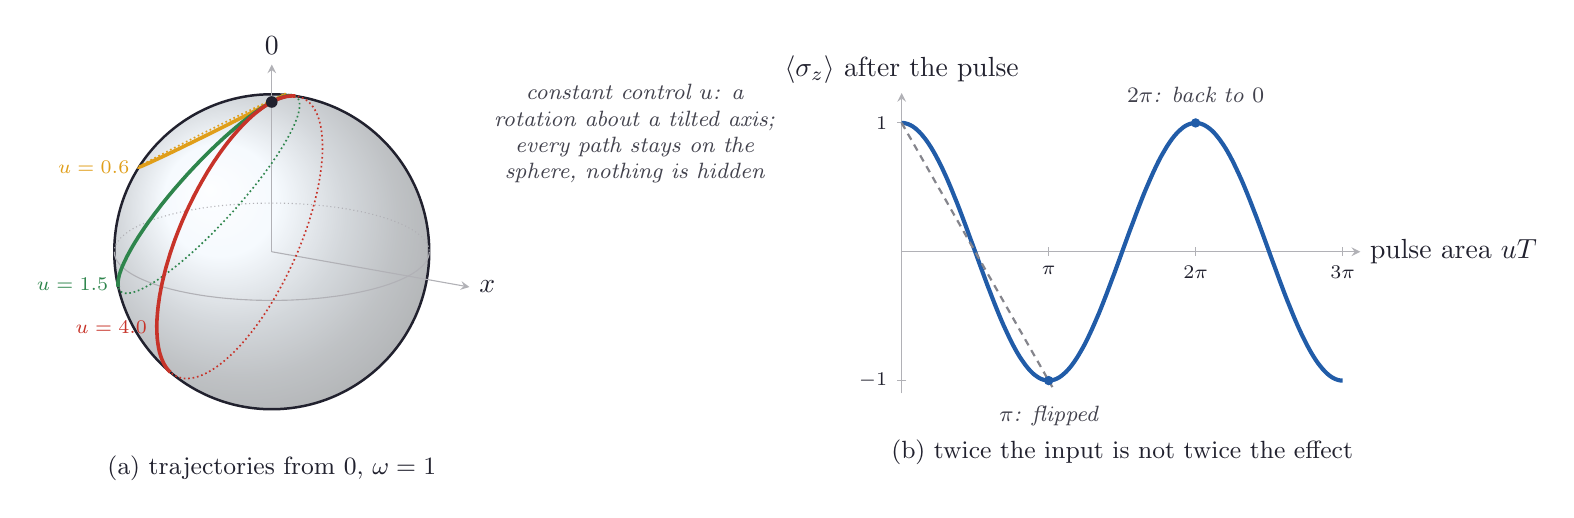
\begin{tikzpicture}[ink/.style={line width=0.9pt, ndInk}, faint/.style={line width=0.4pt, ndInk!35}, dashedink/.style={line width=0.5pt, ndInk!55, dash pattern=on 2.5pt off 2pt}, vec/.style={->, >=stealth, line width=1.2pt}, note/.style={font=\footnotesize\itshape, text=ndInk!85, align=center}, pointer/.style={->, >=stealth, line width=0.4pt, ndInk!60, shorten >=2pt, shorten <=1pt}, dot/.style={circle, fill=ndInk, inner sep=0pt, minimum size=3.4pt}, wash/.style={fill=ndSky, fill opacity=0.55}, every node/.style={text=ndInk}]
\definecolor{ndInk}{rgb}{0.13,0.13,0.18}
\definecolor{ndPaper}{rgb}{0.99,0.96,0.88}
\definecolor{ndSky}{rgb}{0.84,0.91,0.98}
\definecolor{ndRose}{rgb}{0.98,0.86,0.84}
\definecolor{ndBlue}{rgb}{0.13,0.36,0.66}
\definecolor{ndRed}{rgb}{0.78,0.20,0.16}
\definecolor{ndGold}{rgb}{0.88,0.62,0.10}
\definecolor{ndGreen}{rgb}{0.18,0.52,0.30}
\shade[ball color=ndSky!70!white, opacity=0.45] (0.000,0.000) circle (2.000);
\draw[ink] (0.000,0.000) circle (2.000);
\draw[faint] (-2.000,0.000) -- (-1.999,-0.016) -- (-1.997,-0.032) -- (-1.994,-0.048) -- (-1.989,-0.065) -- (-1.983,-0.081) -- (-1.975,-0.097) -- (-1.967,-0.113) -- (-1.956,-0.128) -- (-1.945,-0.144) -- (-1.932,-0.160) -- (-1.918,-0.176) -- (-1.902,-0.191) -- (-1.885,-0.206) -- (-1.867,-0.221) -- (-1.848,-0.237) -- (-1.827,-0.251) -- (-1.805,-0.266) -- (-1.782,-0.281) -- (-1.758,-0.295) -- (-1.732,-0.309) -- (-1.705,-0.323) -- (-1.677,-0.337) -- (-1.648,-0.350) -- (-1.618,-0.363) -- (-1.587,-0.376) -- (-1.554,-0.389) -- (-1.521,-0.401) -- (-1.486,-0.414) -- (-1.451,-0.425) -- (-1.414,-0.437) -- (-1.377,-0.448) -- (-1.338,-0.459) -- (-1.299,-0.470) -- (-1.259,-0.480) -- (-1.218,-0.490) -- (-1.176,-0.500) -- (-1.133,-0.509) -- (-1.089,-0.518) -- (-1.045,-0.527) -- (-1.000,-0.535) -- (-0.954,-0.543) -- (-0.908,-0.551) -- (-0.861,-0.558) -- (-0.813,-0.565) -- (-0.765,-0.571) -- (-0.717,-0.577) -- (-0.668,-0.583) -- (-0.618,-0.588) -- (-0.568,-0.593) -- (-0.518,-0.597) -- (-0.467,-0.601) -- (-0.416,-0.605) -- (-0.364,-0.608) -- (-0.313,-0.610) -- (-0.261,-0.613) -- (-0.209,-0.615) -- (-0.157,-0.616) -- (-0.105,-0.617) -- (-0.052,-0.618) -- (-0.000,-0.618) -- (0.052,-0.618) -- (0.105,-0.617) -- (0.157,-0.616) -- (0.209,-0.615) -- (0.261,-0.613) -- (0.313,-0.610) -- (0.364,-0.608) -- (0.416,-0.605) -- (0.467,-0.601) -- (0.518,-0.597) -- (0.568,-0.593) -- (0.618,-0.588) -- (0.668,-0.583) -- (0.717,-0.577) -- (0.765,-0.571) -- (0.813,-0.565) -- (0.861,-0.558) -- (0.908,-0.551) -- (0.954,-0.543) -- (1.000,-0.535) -- (1.045,-0.527) -- (1.089,-0.518) -- (1.133,-0.509) -- (1.176,-0.500) -- (1.218,-0.490) -- (1.259,-0.480) -- (1.299,-0.470) -- (1.338,-0.459) -- (1.377,-0.448) -- (1.414,-0.437) -- (1.451,-0.425) -- (1.486,-0.414) -- (1.521,-0.401) -- (1.554,-0.389) -- (1.587,-0.376) -- (1.618,-0.363) -- (1.648,-0.350) -- (1.677,-0.337) -- (1.705,-0.323) -- (1.732,-0.309) -- (1.758,-0.295) -- (1.782,-0.281) -- (1.805,-0.266) -- (1.827,-0.251) -- (1.848,-0.237) -- (1.867,-0.221) -- (1.885,-0.206) -- (1.902,-0.191) -- (1.918,-0.176) -- (1.932,-0.160) -- (1.945,-0.144) -- (1.956,-0.128) -- (1.967,-0.113) -- (1.975,-0.097) -- (1.983,-0.081) -- (1.989,-0.065) -- (1.994,-0.048) -- (1.997,-0.032) -- (1.999,-0.016) -- (2.000,-0.000);
\draw[faint, densely dotted] (1.000,0.535) -- (0.954,0.543) -- (0.908,0.551) -- (0.861,0.558) -- (0.813,0.565) -- (0.765,0.571) -- (0.717,0.577) -- (0.668,0.583) -- (0.618,0.588) -- (0.568,0.593) -- (0.518,0.597) -- (0.467,0.601) -- (0.416,0.605) -- (0.364,0.608) -- (0.313,0.610) -- (0.261,0.613) -- (0.209,0.615) -- (0.157,0.616) -- (0.105,0.617) -- (0.052,0.618) -- (0.000,0.618) -- (-0.052,0.618) -- (-0.105,0.617) -- (-0.157,0.616) -- (-0.209,0.615) -- (-0.261,0.613) -- (-0.313,0.610) -- (-0.364,0.608) -- (-0.416,0.605) -- (-0.467,0.601) -- (-0.518,0.597) -- (-0.568,0.593) -- (-0.618,0.588) -- (-0.668,0.583) -- (-0.717,0.577) -- (-0.765,0.571) -- (-0.813,0.565) -- (-0.861,0.558) -- (-0.908,0.551) -- (-0.954,0.543) -- (-1.000,0.535) -- (-1.045,0.527) -- (-1.089,0.518) -- (-1.133,0.509) -- (-1.176,0.500) -- (-1.218,0.490) -- (-1.259,0.480) -- (-1.299,0.470) -- (-1.338,0.459) -- (-1.377,0.448) -- (-1.414,0.437) -- (-1.451,0.425) -- (-1.486,0.414) -- (-1.521,0.401) -- (-1.554,0.389) -- (-1.587,0.376) -- (-1.618,0.363) -- (-1.648,0.350) -- (-1.677,0.337) -- (-1.705,0.323) -- (-1.732,0.309) -- (-1.758,0.295) -- (-1.782,0.281) -- (-1.805,0.266) -- (-1.827,0.251) -- (-1.848,0.237) -- (-1.867,0.221) -- (-1.885,0.206) -- (-1.902,0.191) -- (-1.918,0.176) -- (-1.932,0.160) -- (-1.945,0.144) -- (-1.956,0.128) -- (-1.967,0.113) -- (-1.975,0.097) -- (-1.983,0.081) -- (-1.989,0.065) -- (-1.994,0.048) -- (-1.997,0.032) -- (-1.999,0.016);
\draw[faint, densely dotted] (1.999,0.016) -- (1.997,0.032) -- (1.994,0.048) -- (1.989,0.065) -- (1.983,0.081) -- (1.975,0.097) -- (1.967,0.113) -- (1.956,0.128) -- (1.945,0.144) -- (1.932,0.160) -- (1.918,0.176) -- (1.902,0.191) -- (1.885,0.206) -- (1.867,0.221) -- (1.848,0.237) -- (1.827,0.251) -- (1.805,0.266) -- (1.782,0.281) -- (1.758,0.295) -- (1.732,0.309) -- (1.705,0.323) -- (1.677,0.337) -- (1.648,0.350) -- (1.618,0.363) -- (1.587,0.376) -- (1.554,0.389) -- (1.521,0.401) -- (1.486,0.414) -- (1.451,0.425) -- (1.414,0.437) -- (1.377,0.448) -- (1.338,0.459) -- (1.299,0.470) -- (1.259,0.480) -- (1.218,0.490) -- (1.176,0.500) -- (1.133,0.509) -- (1.089,0.518) -- (1.045,0.527) -- (1.000,0.535);
\draw[faint, ->, >=stealth] (0.000,0.000) -- (0.000,2.378) node[above, text=ndInk] {$\ket0$};
\draw[faint, ->, >=stealth] (0.000,0.000) -- (2.511,-0.448) node[right, text=ndInk] {$x$};
\draw[line width=1.3pt, ndGold] (0.000,1.902) -- (-0.014,1.895) -- (-0.028,1.887) -- (-0.043,1.879) -- (-0.058,1.871) -- (-0.074,1.863) -- (-0.090,1.854) -- (-0.107,1.846) -- (-0.124,1.837) -- (-0.142,1.827) -- (-0.160,1.818) -- (-0.178,1.808) -- (-0.197,1.799) -- (-0.217,1.789) -- (-0.236,1.778) -- (-0.256,1.768) -- (-0.277,1.758) -- (-0.297,1.747) -- (-0.318,1.736) -- (-0.340,1.725) -- (-0.361,1.714) -- (-0.383,1.703) -- (-0.406,1.692) -- (-0.428,1.680) -- (-0.451,1.669) -- (-0.474,1.657) -- (-0.497,1.646) -- (-0.520,1.634) -- (-0.543,1.622) -- (-0.567,1.610) -- (-0.591,1.598) -- (-0.614,1.586) -- (-0.638,1.574) -- (-0.662,1.562) -- (-0.687,1.550) -- (-0.711,1.538) -- (-0.735,1.526) -- (-0.759,1.514) -- (-0.783,1.502) -- (-0.807,1.490) -- (-0.832,1.478) -- (-0.856,1.466) -- (-0.880,1.454) -- (-0.904,1.442) -- (-0.928,1.431) -- (-0.951,1.419) -- (-0.975,1.407) -- (-0.999,1.396) -- (-1.022,1.384) -- (-1.045,1.373) -- (-1.068,1.362) -- (-1.091,1.351) -- (-1.113,1.340) -- (-1.136,1.329) -- (-1.158,1.318) -- (-1.179,1.307) -- (-1.201,1.297) -- (-1.222,1.287) -- (-1.243,1.277) -- (-1.263,1.267) -- (-1.284,1.257) -- (-1.303,1.248) -- (-1.323,1.238) -- (-1.342,1.229) -- (-1.361,1.220) -- (-1.379,1.212) -- (-1.397,1.203) -- (-1.414,1.195) -- (-1.431,1.187) -- (-1.447,1.179) -- (-1.463,1.172) -- (-1.479,1.165) -- (-1.494,1.158) -- (-1.509,1.151) -- (-1.523,1.144) -- (-1.536,1.138) -- (-1.549,1.132) -- (-1.561,1.127) -- (-1.573,1.121) -- (-1.585,1.116) -- (-1.595,1.111) -- (-1.605,1.107) -- (-1.615,1.103) -- (-1.624,1.099) -- (-1.632,1.095) -- (-1.640,1.092) -- (-1.647,1.089) -- (-1.654,1.086) -- (-1.660,1.084) -- (-1.665,1.082) -- (-1.670,1.080) -- (-1.674,1.079) -- (-1.678,1.077) -- (-1.680,1.077) -- (-1.683,1.076) -- (-1.684,1.076) -- (-1.685,1.076) -- (-1.685,1.077);
\draw[line width=1.3pt, ndGold] (0.156,1.994) -- (0.157,1.994) -- (0.157,1.993) -- (0.156,1.992) -- (0.155,1.991) -- (0.153,1.989) -- (0.151,1.987) -- (0.147,1.985) -- (0.143,1.983) -- (0.139,1.980) -- (0.134,1.977) -- (0.128,1.973) -- (0.122,1.969) -- (0.115,1.965) -- (0.107,1.961) -- (0.099,1.956) -- (0.091,1.952) -- (0.081,1.946) -- (0.071,1.941) -- (0.061,1.935) -- (0.050,1.929) -- (0.038,1.923) -- (0.026,1.916) -- (0.013,1.909) -- (0.000,1.902);
\draw[line width=0.6pt, ndGold, densely dotted] (-1.685,1.077) -- (-1.684,1.078) -- (-1.682,1.080) -- (-1.680,1.082) -- (-1.677,1.084) -- (-1.674,1.086) -- (-1.670,1.089) -- (-1.665,1.092) -- (-1.659,1.095) -- (-1.653,1.099) -- (-1.647,1.102) -- (-1.640,1.107) -- (-1.632,1.111) -- (-1.623,1.116) -- (-1.614,1.121) -- (-1.605,1.126) -- (-1.594,1.132) -- (-1.584,1.138) -- (-1.572,1.144) -- (-1.560,1.150) -- (-1.548,1.157) -- (-1.535,1.164) -- (-1.521,1.171) -- (-1.507,1.179) -- (-1.493,1.187) -- (-1.478,1.195) -- (-1.462,1.203) -- (-1.446,1.211) -- (-1.430,1.220) -- (-1.413,1.229) -- (-1.395,1.238) -- (-1.377,1.247) -- (-1.359,1.257) -- (-1.340,1.266) -- (-1.321,1.276) -- (-1.302,1.286) -- (-1.282,1.297) -- (-1.262,1.307) -- (-1.241,1.318) -- (-1.220,1.328) -- (-1.199,1.339) -- (-1.178,1.350) -- (-1.156,1.361) -- (-1.134,1.372) -- (-1.112,1.384) -- (-1.089,1.395) -- (-1.066,1.407) -- (-1.043,1.418) -- (-1.020,1.430) -- (-0.997,1.442) -- (-0.973,1.454) -- (-0.950,1.466) -- (-0.926,1.478) -- (-0.902,1.489) -- (-0.878,1.502) -- (-0.854,1.514) -- (-0.830,1.526) -- (-0.806,1.538) -- (-0.781,1.550) -- (-0.757,1.562) -- (-0.733,1.574) -- (-0.709,1.586) -- (-0.685,1.598) -- (-0.660,1.610) -- (-0.636,1.622) -- (-0.612,1.633) -- (-0.589,1.645) -- (-0.565,1.657) -- (-0.541,1.668) -- (-0.518,1.680) -- (-0.495,1.691) -- (-0.472,1.703) -- (-0.449,1.714) -- (-0.426,1.725) -- (-0.404,1.736) -- (-0.382,1.747) -- (-0.360,1.757) -- (-0.338,1.768) -- (-0.317,1.778) -- (-0.296,1.788) -- (-0.275,1.798) -- (-0.255,1.808) -- (-0.235,1.818) -- (-0.215,1.827) -- (-0.196,1.836) -- (-0.177,1.845) -- (-0.158,1.854) -- (-0.140,1.862) -- (-0.123,1.871) -- (-0.106,1.879) -- (-0.089,1.887) -- (-0.073,1.894) -- (-0.057,1.902) -- (-0.042,1.909) -- (-0.027,1.916) -- (-0.013,1.922) -- (0.001,1.929) -- (0.014,1.935) -- (0.027,1.941) -- (0.039,1.946) -- (0.051,1.951) -- (0.062,1.956) -- (0.072,1.961) -- (0.082,1.965) -- (0.091,1.969) -- (0.100,1.973) -- (0.108,1.976) -- (0.116,1.980) -- (0.122,1.982) -- (0.129,1.985) -- (0.134,1.987) -- (0.139,1.989) -- (0.144,1.991) -- (0.148,1.992) -- (0.151,1.993) -- (0.153,1.994) -- (0.155,1.994);
\node[font=\scriptsize, text=ndGold, anchor=east] at (-1.685,1.077) {$u=0.6$};
\draw[line width=1.3pt, ndGreen] (0.000,1.902) -- (-0.022,1.890) -- (-0.045,1.877) -- (-0.068,1.863) -- (-0.092,1.849) -- (-0.116,1.834) -- (-0.141,1.818) -- (-0.166,1.801) -- (-0.191,1.783) -- (-0.217,1.765) -- (-0.244,1.746) -- (-0.270,1.726) -- (-0.298,1.706) -- (-0.325,1.685) -- (-0.353,1.663) -- (-0.381,1.641) -- (-0.409,1.618) -- (-0.438,1.594) -- (-0.467,1.570) -- (-0.496,1.545) -- (-0.526,1.520) -- (-0.555,1.494) -- (-0.585,1.468) -- (-0.615,1.441) -- (-0.645,1.413) -- (-0.675,1.385) -- (-0.705,1.357) -- (-0.735,1.328) -- (-0.766,1.299) -- (-0.796,1.269) -- (-0.826,1.240) -- (-0.857,1.209) -- (-0.887,1.179) -- (-0.917,1.148) -- (-0.947,1.116) -- (-0.977,1.085) -- (-1.007,1.053) -- (-1.037,1.021) -- (-1.067,0.989) -- (-1.096,0.956) -- (-1.125,0.924) -- (-1.154,0.891) -- (-1.183,0.858) -- (-1.211,0.826) -- (-1.240,0.793) -- (-1.267,0.760) -- (-1.295,0.727) -- (-1.322,0.694) -- (-1.349,0.661) -- (-1.376,0.628) -- (-1.402,0.595) -- (-1.427,0.562) -- (-1.452,0.529) -- (-1.477,0.497) -- (-1.502,0.464) -- (-1.525,0.432) -- (-1.549,0.400) -- (-1.572,0.369) -- (-1.594,0.337) -- (-1.616,0.306) -- (-1.637,0.275) -- (-1.657,0.244) -- (-1.677,0.214) -- (-1.697,0.184) -- (-1.715,0.154) -- (-1.734,0.125) -- (-1.751,0.096) -- (-1.768,0.068) -- (-1.784,0.040) -- (-1.799,0.013) -- (-1.814,-0.014) -- (-1.828,-0.040) -- (-1.842,-0.066) -- (-1.854,-0.092) -- (-1.866,-0.116) -- (-1.877,-0.140) -- (-1.888,-0.164) -- (-1.898,-0.187) -- (-1.907,-0.209) -- (-1.915,-0.231) -- (-1.922,-0.252) -- (-1.929,-0.272) -- (-1.935,-0.292) -- (-1.940,-0.311) -- (-1.944,-0.329) -- (-1.947,-0.346) -- (-1.950,-0.363) -- (-1.952,-0.379) -- (-1.953,-0.394) -- (-1.953,-0.409) -- (-1.953,-0.422) -- (-1.951,-0.435) -- (-1.949,-0.447);
\draw[line width=1.3pt, ndGreen] (0.258,1.983) -- (0.246,1.984) -- (0.233,1.983) -- (0.219,1.982) -- (0.204,1.980) -- (0.189,1.978) -- (0.173,1.974) -- (0.156,1.969) -- (0.139,1.964) -- (0.121,1.957) -- (0.102,1.950) -- (0.083,1.942) -- (0.063,1.934) -- (0.043,1.924) -- (0.022,1.913) -- (0.000,1.902);
\draw[line width=0.6pt, ndGreen, densely dotted] (-1.946,-0.458) -- (-1.943,-0.469) -- (-1.938,-0.478) -- (-1.933,-0.487) -- (-1.927,-0.495) -- (-1.920,-0.502) -- (-1.913,-0.508) -- (-1.904,-0.514) -- (-1.895,-0.518) -- (-1.885,-0.522) -- (-1.874,-0.525) -- (-1.863,-0.527) -- (-1.851,-0.528) -- (-1.838,-0.528) -- (-1.825,-0.527) -- (-1.810,-0.526) -- (-1.795,-0.523) -- (-1.780,-0.520) -- (-1.763,-0.516) -- (-1.746,-0.511) -- (-1.729,-0.505) -- (-1.710,-0.498) -- (-1.691,-0.491) -- (-1.672,-0.482) -- (-1.652,-0.473) -- (-1.631,-0.463) -- (-1.610,-0.452) -- (-1.588,-0.440) -- (-1.565,-0.428) -- (-1.542,-0.415) -- (-1.519,-0.400) -- (-1.495,-0.386) -- (-1.471,-0.370) -- (-1.446,-0.354) -- (-1.420,-0.336) -- (-1.395,-0.318) -- (-1.368,-0.300) -- (-1.342,-0.281) -- (-1.315,-0.260) -- (-1.288,-0.240) -- (-1.260,-0.218) -- (-1.232,-0.196) -- (-1.204,-0.174) -- (-1.175,-0.150) -- (-1.146,-0.127) -- (-1.117,-0.102) -- (-1.088,-0.077) -- (-1.058,-0.051) -- (-1.029,-0.025) -- (-0.999,0.001) -- (-0.969,0.029) -- (-0.939,0.056) -- (-0.909,0.084) -- (-0.879,0.113) -- (-0.848,0.142) -- (-0.818,0.171) -- (-0.788,0.201) -- (-0.757,0.231) -- (-0.727,0.262) -- (-0.697,0.293) -- (-0.667,0.324) -- (-0.637,0.355) -- (-0.607,0.387) -- (-0.577,0.419) -- (-0.547,0.451) -- (-0.518,0.483) -- (-0.488,0.516) -- (-0.459,0.548) -- (-0.430,0.581) -- (-0.402,0.614) -- (-0.373,0.647) -- (-0.345,0.680) -- (-0.318,0.713) -- (-0.290,0.746) -- (-0.263,0.779) -- (-0.236,0.812) -- (-0.210,0.845) -- (-0.184,0.877) -- (-0.159,0.910) -- (-0.134,0.943) -- (-0.109,0.975) -- (-0.085,1.007) -- (-0.062,1.040) -- (-0.039,1.071) -- (-0.016,1.103) -- (0.006,1.134) -- (0.027,1.166) -- (0.048,1.196) -- (0.069,1.227) -- (0.088,1.257) -- (0.107,1.287) -- (0.126,1.316) -- (0.144,1.345) -- (0.161,1.374) -- (0.177,1.402) -- (0.193,1.429) -- (0.208,1.456) -- (0.223,1.483) -- (0.236,1.509) -- (0.249,1.535) -- (0.262,1.560) -- (0.273,1.584) -- (0.284,1.608) -- (0.294,1.631) -- (0.303,1.654) -- (0.312,1.676) -- (0.320,1.697) -- (0.327,1.718) -- (0.333,1.738) -- (0.338,1.757) -- (0.343,1.776) -- (0.347,1.793) -- (0.350,1.811) -- (0.352,1.827) -- (0.354,1.843) -- (0.354,1.857) -- (0.354,1.871) -- (0.353,1.885) -- (0.352,1.897) -- (0.349,1.909) -- (0.346,1.920) -- (0.342,1.930) -- (0.337,1.939) -- (0.331,1.947) -- (0.325,1.955) -- (0.318,1.961) -- (0.310,1.967) -- (0.301,1.972) -- (0.291,1.976) -- (0.281,1.979) -- (0.270,1.982);
\node[font=\scriptsize, text=ndGreen, anchor=east] at (-1.953,-0.409) {$u=1.5$};
\draw[line width=1.3pt, ndRed] (0.000,1.902) -- (-0.026,1.888) -- (-0.052,1.872) -- (-0.078,1.856) -- (-0.104,1.838) -- (-0.131,1.819) -- (-0.157,1.799) -- (-0.184,1.778) -- (-0.212,1.756) -- (-0.239,1.733) -- (-0.266,1.708) -- (-0.294,1.683) -- (-0.321,1.656) -- (-0.349,1.629) -- (-0.376,1.600) -- (-0.404,1.571) -- (-0.432,1.540) -- (-0.459,1.509) -- (-0.487,1.477) -- (-0.514,1.444) -- (-0.542,1.410) -- (-0.569,1.375) -- (-0.597,1.339) -- (-0.624,1.302) -- (-0.651,1.265) -- (-0.678,1.227) -- (-0.704,1.188) -- (-0.731,1.149) -- (-0.757,1.109) -- (-0.783,1.068) -- (-0.809,1.027) -- (-0.834,0.985) -- (-0.859,0.942) -- (-0.884,0.899) -- (-0.908,0.856) -- (-0.933,0.812) -- (-0.956,0.767) -- (-0.980,0.723) -- (-1.003,0.677) -- (-1.025,0.632) -- (-1.048,0.586) -- (-1.069,0.540) -- (-1.091,0.494) -- (-1.111,0.447) -- (-1.132,0.400) -- (-1.152,0.353) -- (-1.171,0.306) -- (-1.190,0.259) -- (-1.208,0.212) -- (-1.226,0.165) -- (-1.243,0.118) -- (-1.259,0.071) -- (-1.275,0.024) -- (-1.291,-0.023) -- (-1.305,-0.070) -- (-1.319,-0.117) -- (-1.333,-0.163) -- (-1.346,-0.209) -- (-1.358,-0.255) -- (-1.369,-0.301) -- (-1.380,-0.346) -- (-1.391,-0.391) -- (-1.400,-0.435) -- (-1.409,-0.479) -- (-1.417,-0.523) -- (-1.425,-0.566) -- (-1.431,-0.609) -- (-1.437,-0.651) -- (-1.443,-0.692) -- (-1.447,-0.733) -- (-1.451,-0.773) -- (-1.454,-0.813) -- (-1.457,-0.852) -- (-1.459,-0.890) -- (-1.460,-0.927) -- (-1.460,-0.964) -- (-1.459,-1.000) -- (-1.458,-1.035) -- (-1.456,-1.069) -- (-1.454,-1.102) -- (-1.450,-1.135) -- (-1.446,-1.166) -- (-1.441,-1.197) -- (-1.436,-1.226) -- (-1.430,-1.255) -- (-1.423,-1.283) -- (-1.415,-1.309) -- (-1.407,-1.335) -- (-1.398,-1.359) -- (-1.388,-1.383) -- (-1.378,-1.405) -- (-1.367,-1.427) -- (-1.355,-1.447) -- (-1.343,-1.466) -- (-1.330,-1.484) -- (-1.316,-1.501) -- (-1.302,-1.516) -- (-1.287,-1.531);
\draw[line width=1.3pt, ndRed] (0.302,1.977) -- (0.281,1.978) -- (0.260,1.979) -- (0.238,1.978) -- (0.216,1.976) -- (0.194,1.973) -- (0.171,1.968) -- (0.147,1.962) -- (0.124,1.955) -- (0.100,1.947) -- (0.075,1.938) -- (0.050,1.927) -- (0.025,1.915) -- (0.000,1.902);
\draw[line width=0.6pt, ndRed, densely dotted] (-1.271,-1.544) -- (-1.255,-1.556) -- (-1.239,-1.567) -- (-1.221,-1.576) -- (-1.203,-1.585) -- (-1.185,-1.592) -- (-1.166,-1.598) -- (-1.147,-1.603) -- (-1.127,-1.606) -- (-1.106,-1.609) -- (-1.085,-1.610) -- (-1.064,-1.609) -- (-1.042,-1.608) -- (-1.020,-1.605) -- (-0.997,-1.601) -- (-0.974,-1.596) -- (-0.951,-1.590) -- (-0.927,-1.582) -- (-0.902,-1.573) -- (-0.878,-1.563) -- (-0.853,-1.552) -- (-0.828,-1.540) -- (-0.802,-1.526) -- (-0.777,-1.511) -- (-0.750,-1.495) -- (-0.724,-1.478) -- (-0.698,-1.460) -- (-0.671,-1.440) -- (-0.644,-1.420) -- (-0.617,-1.398) -- (-0.590,-1.375) -- (-0.563,-1.351) -- (-0.535,-1.326) -- (-0.508,-1.300) -- (-0.480,-1.273) -- (-0.453,-1.245) -- (-0.425,-1.216) -- (-0.397,-1.187) -- (-0.370,-1.156) -- (-0.342,-1.124) -- (-0.314,-1.091) -- (-0.287,-1.057) -- (-0.259,-1.023) -- (-0.232,-0.988) -- (-0.205,-0.952) -- (-0.178,-0.915) -- (-0.151,-0.877) -- (-0.124,-0.839) -- (-0.098,-0.800) -- (-0.071,-0.760) -- (-0.045,-0.719) -- (-0.019,-0.678) -- (0.006,-0.637) -- (0.032,-0.594) -- (0.057,-0.552) -- (0.081,-0.508) -- (0.105,-0.465) -- (0.129,-0.420) -- (0.153,-0.376) -- (0.176,-0.331) -- (0.199,-0.285) -- (0.221,-0.240) -- (0.243,-0.194) -- (0.265,-0.148) -- (0.286,-0.101) -- (0.307,-0.054) -- (0.327,-0.008) -- (0.346,0.039) -- (0.365,0.086) -- (0.384,0.134) -- (0.402,0.181) -- (0.419,0.228) -- (0.436,0.275) -- (0.452,0.322) -- (0.468,0.369) -- (0.483,0.416) -- (0.497,0.463) -- (0.511,0.509) -- (0.524,0.555) -- (0.537,0.601) -- (0.549,0.647) -- (0.560,0.693) -- (0.570,0.738) -- (0.580,0.782) -- (0.590,0.827) -- (0.598,0.870) -- (0.606,0.914) -- (0.613,0.957) -- (0.619,0.999) -- (0.625,1.041) -- (0.630,1.082) -- (0.634,1.122) -- (0.638,1.162) -- (0.641,1.201) -- (0.643,1.240) -- (0.644,1.278) -- (0.645,1.315) -- (0.645,1.351) -- (0.644,1.386) -- (0.642,1.421) -- (0.640,1.455) -- (0.637,1.488) -- (0.633,1.520) -- (0.629,1.551) -- (0.624,1.581) -- (0.618,1.610) -- (0.611,1.638) -- (0.604,1.665) -- (0.596,1.691) -- (0.587,1.716) -- (0.578,1.740) -- (0.568,1.763) -- (0.557,1.785) -- (0.546,1.806) -- (0.534,1.826) -- (0.521,1.844) -- (0.508,1.862) -- (0.494,1.878) -- (0.479,1.893) -- (0.464,1.907) -- (0.448,1.919) -- (0.432,1.931) -- (0.415,1.941) -- (0.397,1.950) -- (0.379,1.958) -- (0.361,1.964) -- (0.341,1.970) -- (0.322,1.974);
\node[font=\scriptsize, text=ndRed, anchor=east] at (-1.460,-0.964) {$u=4.0$};
\node[dot, minimum size=4.2pt] at (0.000,1.902) {};
\node[note, anchor=west] at (2.7,1.5) {constant control $u$: a\\ rotation about a tilted axis;\\ every path stays on the\\ sphere, nothing is hidden};
\node[font=\small] at (0,-2.75) {(a) trajectories from $\ket0$, $\omega=1$};
\draw[faint, ->, >=stealth] (8.000,0.000) -- (13.824,0.000) node[right, text=ndInk] {pulse area $uT$};
\draw[faint, ->, >=stealth] (8.000,-1.800) -- (8.000,2.016) node[above, text=ndInk] {$\langle\sigma_z\rangle$ after the pulse};
\draw[faint] (9.867,0.060) -- (9.867,-0.060) node[below, font=\scriptsize, text=ndInk] {$\pi$};
\draw[faint] (11.733,0.060) -- (11.733,-0.060) node[below, font=\scriptsize, text=ndInk] {$2\pi$};
\draw[faint] (13.600,0.060) -- (13.600,-0.060) node[below, font=\scriptsize, text=ndInk] {$3\pi$};
\draw[faint] (8.060,-1.636) -- (7.940,-1.636) node[left, font=\scriptsize, text=ndInk] {$-1$};
\draw[faint] (8.060,1.636) -- (7.940,1.636) node[left, font=\scriptsize, text=ndInk] {$1$};
\draw[line width=1.5pt, ndBlue] (8.000,1.636) -- (8.028,1.635) -- (8.056,1.629) -- (8.084,1.620) -- (8.113,1.607) -- (8.141,1.591) -- (8.169,1.571) -- (8.197,1.547) -- (8.225,1.520) -- (8.253,1.490) -- (8.281,1.456) -- (8.310,1.419) -- (8.338,1.379) -- (8.366,1.336) -- (8.394,1.290) -- (8.422,1.241) -- (8.450,1.189) -- (8.478,1.134) -- (8.507,1.077) -- (8.535,1.017) -- (8.563,0.956) -- (8.591,0.892) -- (8.619,0.826) -- (8.647,0.758) -- (8.675,0.688) -- (8.704,0.617) -- (8.732,0.545) -- (8.760,0.471) -- (8.788,0.396) -- (8.816,0.321) -- (8.844,0.244) -- (8.872,0.168) -- (8.901,0.090) -- (8.929,0.013) -- (8.957,-0.065) -- (8.985,-0.142) -- (9.013,-0.219) -- (9.041,-0.295) -- (9.069,-0.371) -- (9.097,-0.446) -- (9.126,-0.520) -- (9.154,-0.593) -- (9.182,-0.665) -- (9.210,-0.735) -- (9.238,-0.803) -- (9.266,-0.870) -- (9.294,-0.934) -- (9.323,-0.997) -- (9.351,-1.057) -- (9.379,-1.115) -- (9.407,-1.171) -- (9.435,-1.224) -- (9.463,-1.274) -- (9.491,-1.321) -- (9.520,-1.365) -- (9.548,-1.406) -- (9.576,-1.444) -- (9.604,-1.479) -- (9.632,-1.511) -- (9.660,-1.539) -- (9.688,-1.563) -- (9.717,-1.584) -- (9.745,-1.602) -- (9.773,-1.616) -- (9.801,-1.626) -- (9.829,-1.633) -- (9.857,-1.636) -- (9.885,-1.636) -- (9.914,-1.631) -- (9.942,-1.623) -- (9.970,-1.612) -- (9.998,-1.597) -- (10.026,-1.578) -- (10.054,-1.555) -- (10.082,-1.530) -- (10.111,-1.500) -- (10.139,-1.468) -- (10.167,-1.432) -- (10.195,-1.393) -- (10.223,-1.351) -- (10.251,-1.305) -- (10.279,-1.257) -- (10.308,-1.206) -- (10.336,-1.153) -- (10.364,-1.096) -- (10.392,-1.037) -- (10.420,-0.976) -- (10.448,-0.913) -- (10.476,-0.848) -- (10.505,-0.781) -- (10.533,-0.712) -- (10.561,-0.641) -- (10.589,-0.569) -- (10.617,-0.496) -- (10.645,-0.421) -- (10.673,-0.346) -- (10.702,-0.270) -- (10.730,-0.193) -- (10.758,-0.116) -- (10.786,-0.039) -- (10.814,0.039) -- (10.842,0.116) -- (10.870,0.193) -- (10.898,0.270) -- (10.927,0.346) -- (10.955,0.421) -- (10.983,0.496) -- (11.011,0.569) -- (11.039,0.641) -- (11.067,0.712) -- (11.095,0.781) -- (11.124,0.848) -- (11.152,0.913) -- (11.180,0.976) -- (11.208,1.037) -- (11.236,1.096) -- (11.264,1.153) -- (11.292,1.206) -- (11.321,1.257) -- (11.349,1.305) -- (11.377,1.351) -- (11.405,1.393) -- (11.433,1.432) -- (11.461,1.468) -- (11.489,1.500) -- (11.518,1.530) -- (11.546,1.555) -- (11.574,1.578) -- (11.602,1.597) -- (11.630,1.612) -- (11.658,1.623) -- (11.686,1.631) -- (11.715,1.636) -- (11.743,1.636) -- (11.771,1.633) -- (11.799,1.626) -- (11.827,1.616) -- (11.855,1.602) -- (11.883,1.584) -- (11.912,1.563) -- (11.940,1.539) -- (11.968,1.511) -- (11.996,1.479) -- (12.024,1.444) -- (12.052,1.406) -- (12.080,1.365) -- (12.109,1.321) -- (12.137,1.274) -- (12.165,1.224) -- (12.193,1.171) -- (12.221,1.115) -- (12.249,1.057) -- (12.277,0.997) -- (12.306,0.934) -- (12.334,0.870) -- (12.362,0.803) -- (12.390,0.735) -- (12.418,0.665) -- (12.446,0.593) -- (12.474,0.520) -- (12.503,0.446) -- (12.531,0.371) -- (12.559,0.295) -- (12.587,0.219) -- (12.615,0.142) -- (12.643,0.065) -- (12.671,-0.013) -- (12.699,-0.090) -- (12.728,-0.168) -- (12.756,-0.244) -- (12.784,-0.321) -- (12.812,-0.396) -- (12.840,-0.471) -- (12.868,-0.545) -- (12.896,-0.617) -- (12.925,-0.688) -- (12.953,-0.758) -- (12.981,-0.826) -- (13.009,-0.892) -- (13.037,-0.956) -- (13.065,-1.017) -- (13.093,-1.077) -- (13.122,-1.134) -- (13.150,-1.189) -- (13.178,-1.241) -- (13.206,-1.290) -- (13.234,-1.336) -- (13.262,-1.379) -- (13.290,-1.419) -- (13.319,-1.456) -- (13.347,-1.490) -- (13.375,-1.520) -- (13.403,-1.547) -- (13.431,-1.571) -- (13.459,-1.591) -- (13.487,-1.607) -- (13.516,-1.620) -- (13.544,-1.629) -- (13.572,-1.635) -- (13.600,-1.636);
\draw[dashedink, line width=0.8pt] (8.000,1.636) -- (8.028,1.587) -- (8.056,1.538) -- (8.084,1.488) -- (8.113,1.439) -- (8.141,1.390) -- (8.169,1.340) -- (8.197,1.291) -- (8.225,1.242) -- (8.253,1.192) -- (8.281,1.143) -- (8.310,1.094) -- (8.338,1.044) -- (8.366,0.995) -- (8.394,0.946) -- (8.422,0.896) -- (8.450,0.847) -- (8.478,0.798) -- (8.507,0.748) -- (8.535,0.699) -- (8.563,0.650) -- (8.591,0.600) -- (8.619,0.551) -- (8.647,0.502) -- (8.675,0.452) -- (8.704,0.403) -- (8.732,0.354) -- (8.760,0.304) -- (8.788,0.255) -- (8.816,0.206) -- (8.844,0.156) -- (8.872,0.107) -- (8.901,0.058) -- (8.929,0.008) -- (8.957,-0.041) -- (8.985,-0.090) -- (9.013,-0.140) -- (9.041,-0.189) -- (9.069,-0.238) -- (9.097,-0.288) -- (9.126,-0.337) -- (9.154,-0.386) -- (9.182,-0.436) -- (9.210,-0.485) -- (9.238,-0.534) -- (9.266,-0.584) -- (9.294,-0.633) -- (9.323,-0.683) -- (9.351,-0.732) -- (9.379,-0.781) -- (9.407,-0.831) -- (9.435,-0.880) -- (9.463,-0.929) -- (9.491,-0.979) -- (9.520,-1.028) -- (9.548,-1.077) -- (9.576,-1.127) -- (9.604,-1.176) -- (9.632,-1.225) -- (9.660,-1.275) -- (9.688,-1.324) -- (9.717,-1.373) -- (9.745,-1.423) -- (9.773,-1.472) -- (9.801,-1.521) -- (9.829,-1.571) -- (9.857,-1.620) -- (9.885,-1.669) -- (9.914,-1.719);
\node[dot, fill=ndBlue] at (9.867,-1.636) {};
\node[note, anchor=north] at (9.867,-1.833) {$\pi$: flipped};
\node[dot, fill=ndBlue] at (11.733,1.636) {};
\node[note, anchor=south] at (11.733,1.767) {$2\pi$: back to $\ket0$};
\node[font=\small] at (10.800,-2.550) {(b) twice the input is not twice the effect};
\end{tikzpicture}
}\end{center}
$\mathbf A,\mathbf N$ antisymmetric: rotations. $\mathbf C=\Id$: nothing hidden. Not linear in $u$: $\pi$ flips, $2\pi$ returns.}
\end{frame}

\begin{frame}\ft{Example: a qubit with a hidden defect}
\ona{Now let the same qubit interact with a defect in its environment: a two-level system, such as a charge trap, that we neither drive nor measure, and which itself loses energy into a large bath at the rate $\kappa$ (\Chap~\ref{C.Open}). With an exchange coupling of strength $g$,}
\onp{Qubit $S$, coupled to a defect $T$ that decays into a bath:}
\begin{equation}\label{eq:ch04:hidden}
H(t)=-\tfrac\omega2\big(\sigma_z^S+\sigma_z^T\big)+g\big(\sigma_+^S\sigma_-^T+\sigma_-^S\sigma_+^T\big)+\tfrac{u(t)}2\sigma_x^S,\qquad L=\sqrt\kappa\,\sigma_-^T .
\end{equation}
\ona{The state of qubit and defect together is the coherence vector of two qubits, with $15$ components, and the GKSL equation is again a bilinear system, $\dot{\vec x}=(\mathbf A+u\mathbf N)\vec x+\vec\beta$, now with an affine term from the dissipation. But we measure only the qubit. The three rows of $\mathbf C$ pick the components along $\sigma_x^S$, $\sigma_y^S$ and $\sigma_z^S$, and the other twelve, which describe the defect and its correlations with the qubit, form a \emph{hidden state}: they never appear in the output directly, but they shape its future. Starting with the qubit excited, the excitation passes to the defect and partly comes back before it is lost to the bath, so that the excited population of the qubit revives (Figure~\ref{fig:ch04:hidden}(b)). Since the qubit's state started from $\ket0$ never changes, this population is also the distinguishability of the two initial states, and its revival is the non-Markovian behaviour of \Chap~\ref{C.Open}. The best model of the qubit alone, an exponential decay, misses it, while the bilinear model with the hidden state reproduces it exactly: this is the Markovian embedding of \Chap~\ref{C.Open} again. Hidden does not mean unobservable. Through the dynamics, the readout of the qubit sees $8$ of the $16$ dimensions of the embedded state when $u\equiv0$, and $11$ when the control is used, since in a bilinear system the input also shapes what the output reveals. Computer scientists will recognise the hidden state of a hidden Markov model, or of a recurrent neural network: the observed sequence is generated by a larger state that is never observed directly.}
\ona{\begin{figure}[H]\centering
\resizebox{\linewidth}{!}{% Generated by code/needham.py -- do not edit by hand.
\definecolor{qocA}{rgb}{0.00,0.45,0.70}
\definecolor{qocB}{rgb}{0.90,0.60,0.00}
\definecolor{qocC}{rgb}{0.00,0.62,0.45}
\definecolor{qocD}{rgb}{0.80,0.40,0.00}
\definecolor{qocE}{rgb}{0.80,0.60,0.70}
\definecolor{qocF}{rgb}{0.35,0.70,0.90}
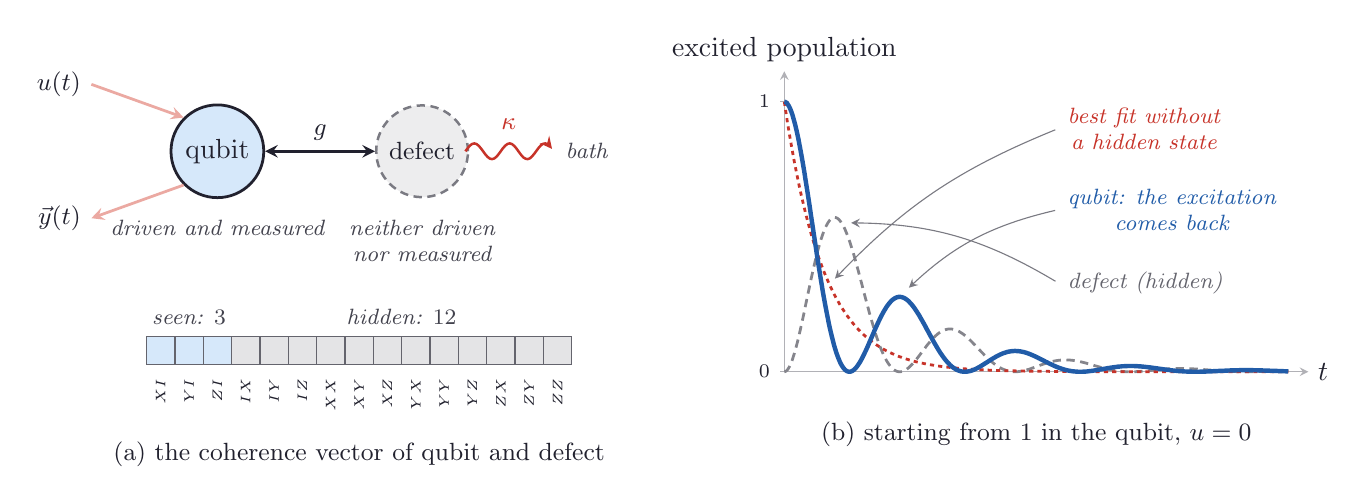
\begin{tikzpicture}[ink/.style={line width=0.9pt, ndInk}, faint/.style={line width=0.4pt, ndInk!35}, dashedink/.style={line width=0.5pt, ndInk!55, dash pattern=on 2.5pt off 2pt}, vec/.style={->, >=stealth, line width=1.2pt}, note/.style={font=\footnotesize\itshape, text=ndInk!85, align=center}, pointer/.style={->, >=stealth, line width=0.4pt, ndInk!60, shorten >=2pt, shorten <=1pt}, dot/.style={circle, fill=ndInk, inner sep=0pt, minimum size=3.4pt}, wash/.style={fill=ndSky, fill opacity=0.55}, every node/.style={text=ndInk}]
\definecolor{ndInk}{rgb}{0.13,0.13,0.18}
\definecolor{ndPaper}{rgb}{0.99,0.96,0.88}
\definecolor{ndSky}{rgb}{0.84,0.91,0.98}
\definecolor{ndRose}{rgb}{0.98,0.86,0.84}
\definecolor{ndBlue}{rgb}{0.13,0.36,0.66}
\definecolor{ndRed}{rgb}{0.78,0.20,0.16}
\definecolor{ndGold}{rgb}{0.88,0.62,0.10}
\definecolor{ndGreen}{rgb}{0.18,0.52,0.30}
\node[circle, draw=ndInk, line width=1.0pt, fill=ndSky, minimum size=1.05cm] (S) at (0,0.6) {qubit};
\node[circle, draw=ndInk!60, line width=0.9pt, dash pattern=on 3pt off 2pt, fill=ndInk!8, minimum size=1.05cm, font=\small] (T) at (2.6,0.6) {defect};
\draw[<->, >=stealth, line width=1.0pt, ndInk] (S) -- node[above, font=\small] {$g$} (T);
\draw[->, >=stealth, line width=0.9pt, ndRed] (3.150,0.600) -- (3.178,0.638) -- (3.206,0.671) -- (3.235,0.693) -- (3.263,0.700) -- (3.291,0.692) -- (3.319,0.670) -- (3.347,0.637) -- (3.376,0.598) -- (3.404,0.560) -- (3.432,0.528) -- (3.460,0.507) -- (3.488,0.500) -- (3.517,0.509) -- (3.545,0.531) -- (3.573,0.565) -- (3.601,0.603) -- (3.629,0.642) -- (3.658,0.673) -- (3.686,0.694) -- (3.714,0.700) -- (3.742,0.691) -- (3.771,0.667) -- (3.799,0.634) -- (3.827,0.595) -- (3.855,0.557) -- (3.883,0.525) -- (3.912,0.506) -- (3.940,0.500) -- (3.968,0.510) -- (3.996,0.534) -- (4.024,0.568) -- (4.053,0.607) -- (4.081,0.645) -- (4.109,0.676) -- (4.137,0.695) -- (4.165,0.700) -- (4.194,0.689) -- (4.222,0.665) -- (4.250,0.630);
\node[font=\small, text=ndRed, above] at (3.7,0.75) {$\kappa$};
\node[note, anchor=west] at (4.3,0.6) {bath};
\draw[->, >=stealth, line width=1.0pt, ndRose!70!ndRed] (-1.6,1.45) node[left, text=ndInk, font=\small] {$u(t)$} -- (S.north west);
\draw[->, >=stealth, line width=1.0pt, ndRose!70!ndRed] (S.south west) -- (-1.6,-0.25) node[left, text=ndInk, font=\small] {$\vec y(t)$};
\node[note, anchor=north] at (0,-0.15) {driven and measured};
\node[note, anchor=north] at (2.6,-0.15) {neither driven\\ nor measured};
\filldraw[fill=ndSky, draw=ndInk!70, line width=0.5pt] (-0.900,-1.75) rectangle (-0.540,-2.11);
\node[font=\tiny, rotate=90, anchor=east] at (-0.720,-2.16) {$XI$};
\filldraw[fill=ndSky, draw=ndInk!70, line width=0.5pt] (-0.540,-1.75) rectangle (-0.180,-2.11);
\node[font=\tiny, rotate=90, anchor=east] at (-0.360,-2.16) {$YI$};
\filldraw[fill=ndSky, draw=ndInk!70, line width=0.5pt] (-0.180,-1.75) rectangle (0.180,-2.11);
\node[font=\tiny, rotate=90, anchor=east] at (-0.000,-2.16) {$ZI$};
\filldraw[fill=ndInk!12, draw=ndInk!70, line width=0.5pt] (0.180,-1.75) rectangle (0.540,-2.11);
\node[font=\tiny, rotate=90, anchor=east] at (0.360,-2.16) {$IX$};
\filldraw[fill=ndInk!12, draw=ndInk!70, line width=0.5pt] (0.540,-1.75) rectangle (0.900,-2.11);
\node[font=\tiny, rotate=90, anchor=east] at (0.720,-2.16) {$IY$};
\filldraw[fill=ndInk!12, draw=ndInk!70, line width=0.5pt] (0.900,-1.75) rectangle (1.260,-2.11);
\node[font=\tiny, rotate=90, anchor=east] at (1.080,-2.16) {$IZ$};
\filldraw[fill=ndInk!12, draw=ndInk!70, line width=0.5pt] (1.260,-1.75) rectangle (1.620,-2.11);
\node[font=\tiny, rotate=90, anchor=east] at (1.440,-2.16) {$XX$};
\filldraw[fill=ndInk!12, draw=ndInk!70, line width=0.5pt] (1.620,-1.75) rectangle (1.980,-2.11);
\node[font=\tiny, rotate=90, anchor=east] at (1.800,-2.16) {$XY$};
\filldraw[fill=ndInk!12, draw=ndInk!70, line width=0.5pt] (1.980,-1.75) rectangle (2.340,-2.11);
\node[font=\tiny, rotate=90, anchor=east] at (2.160,-2.16) {$XZ$};
\filldraw[fill=ndInk!12, draw=ndInk!70, line width=0.5pt] (2.340,-1.75) rectangle (2.700,-2.11);
\node[font=\tiny, rotate=90, anchor=east] at (2.520,-2.16) {$YX$};
\filldraw[fill=ndInk!12, draw=ndInk!70, line width=0.5pt] (2.700,-1.75) rectangle (3.060,-2.11);
\node[font=\tiny, rotate=90, anchor=east] at (2.880,-2.16) {$YY$};
\filldraw[fill=ndInk!12, draw=ndInk!70, line width=0.5pt] (3.060,-1.75) rectangle (3.420,-2.11);
\node[font=\tiny, rotate=90, anchor=east] at (3.240,-2.16) {$YZ$};
\filldraw[fill=ndInk!12, draw=ndInk!70, line width=0.5pt] (3.420,-1.75) rectangle (3.780,-2.11);
\node[font=\tiny, rotate=90, anchor=east] at (3.600,-2.16) {$ZX$};
\filldraw[fill=ndInk!12, draw=ndInk!70, line width=0.5pt] (3.780,-1.75) rectangle (4.140,-2.11);
\node[font=\tiny, rotate=90, anchor=east] at (3.960,-2.16) {$ZY$};
\filldraw[fill=ndInk!12, draw=ndInk!70, line width=0.5pt] (4.140,-1.75) rectangle (4.500,-2.11);
\node[font=\tiny, rotate=90, anchor=east] at (4.320,-2.16) {$ZZ$};
\node[note, anchor=south] at (-0.360,-1.72) {seen: $3$};
\node[note, anchor=south] at (2.340,-1.72) {hidden: $12$};
\node[font=\small] at (1.8,-3.25) {(a) the coherence vector of qubit and defect};
\draw[faint, ->, >=stealth] (7.200,-2.200) -- (13.856,-2.200) node[right, text=ndInk] {$t$};
\draw[faint, ->, >=stealth] (7.200,-2.200) -- (7.200,1.616) node[above, text=ndInk] {excited population};
\draw[faint] (7.260,-2.200) -- (7.140,-2.200) node[left, font=\scriptsize, text=ndInk] {$0$};
\draw[faint] (7.260,1.229) -- (7.140,1.229) node[left, font=\scriptsize, text=ndInk] {$1$};
\draw[line width=1.0pt, ndInk!55, dash pattern=on 3pt off 2pt] (7.200,-2.200) -- (7.213,-2.197) -- (7.226,-2.189) -- (7.238,-2.177) -- (7.251,-2.159) -- (7.264,-2.137) -- (7.277,-2.110) -- (7.290,-2.079) -- (7.303,-2.045) -- (7.315,-2.006) -- (7.328,-1.965) -- (7.341,-1.920) -- (7.354,-1.872) -- (7.367,-1.822) -- (7.380,-1.770) -- (7.392,-1.715) -- (7.405,-1.659) -- (7.418,-1.601) -- (7.431,-1.542) -- (7.444,-1.482) -- (7.457,-1.421) -- (7.469,-1.360) -- (7.482,-1.298) -- (7.495,-1.236) -- (7.508,-1.175) -- (7.521,-1.114) -- (7.533,-1.054) -- (7.546,-0.995) -- (7.559,-0.937) -- (7.572,-0.880) -- (7.585,-0.825) -- (7.598,-0.771) -- (7.610,-0.719) -- (7.623,-0.670) -- (7.636,-0.622) -- (7.649,-0.577) -- (7.662,-0.534) -- (7.675,-0.494) -- (7.687,-0.457) -- (7.700,-0.422) -- (7.713,-0.390) -- (7.726,-0.361) -- (7.739,-0.335) -- (7.752,-0.312) -- (7.764,-0.293) -- (7.777,-0.276) -- (7.790,-0.262) -- (7.803,-0.252) -- (7.816,-0.245) -- (7.828,-0.241) -- (7.841,-0.240) -- (7.854,-0.242) -- (7.867,-0.247) -- (7.880,-0.255) -- (7.893,-0.266) -- (7.905,-0.280) -- (7.918,-0.297) -- (7.931,-0.316) -- (7.944,-0.338) -- (7.957,-0.363) -- (7.970,-0.390) -- (7.982,-0.419) -- (7.995,-0.451) -- (8.008,-0.484) -- (8.021,-0.520) -- (8.034,-0.557) -- (8.046,-0.596) -- (8.059,-0.637) -- (8.072,-0.679) -- (8.085,-0.722) -- (8.098,-0.767) -- (8.111,-0.813) -- (8.123,-0.859) -- (8.136,-0.906) -- (8.149,-0.954) -- (8.162,-1.003) -- (8.175,-1.052) -- (8.188,-1.101) -- (8.200,-1.150) -- (8.213,-1.199) -- (8.226,-1.248) -- (8.239,-1.296) -- (8.252,-1.344) -- (8.265,-1.392) -- (8.277,-1.439) -- (8.290,-1.485) -- (8.303,-1.530) -- (8.316,-1.575) -- (8.329,-1.618) -- (8.341,-1.660) -- (8.354,-1.701) -- (8.367,-1.741) -- (8.380,-1.780) -- (8.393,-1.816) -- (8.406,-1.852) -- (8.418,-1.886) -- (8.431,-1.918) -- (8.444,-1.948) -- (8.457,-1.977) -- (8.470,-2.004) -- (8.483,-2.030) -- (8.495,-2.053) -- (8.508,-2.075) -- (8.521,-2.095) -- (8.534,-2.113) -- (8.547,-2.130) -- (8.560,-2.145) -- (8.572,-2.157) -- (8.585,-2.169) -- (8.598,-2.178) -- (8.611,-2.186) -- (8.624,-2.192) -- (8.636,-2.196) -- (8.649,-2.199) -- (8.662,-2.200) -- (8.675,-2.200) -- (8.688,-2.198) -- (8.701,-2.195) -- (8.713,-2.190) -- (8.726,-2.184) -- (8.739,-2.177) -- (8.752,-2.169) -- (8.765,-2.160) -- (8.778,-2.149) -- (8.790,-2.138) -- (8.803,-2.126) -- (8.816,-2.113) -- (8.829,-2.099) -- (8.842,-2.085) -- (8.855,-2.070) -- (8.867,-2.054) -- (8.880,-2.039) -- (8.893,-2.022) -- (8.906,-2.006) -- (8.919,-1.989) -- (8.931,-1.972) -- (8.944,-1.955) -- (8.957,-1.938) -- (8.970,-1.921) -- (8.983,-1.904) -- (8.996,-1.887) -- (9.008,-1.870) -- (9.021,-1.854) -- (9.034,-1.838) -- (9.047,-1.823) -- (9.060,-1.808) -- (9.073,-1.793) -- (9.085,-1.779) -- (9.098,-1.766) -- (9.111,-1.753) -- (9.124,-1.741) -- (9.137,-1.730) -- (9.149,-1.719) -- (9.162,-1.710) -- (9.175,-1.700) -- (9.188,-1.692) -- (9.201,-1.685) -- (9.214,-1.678) -- (9.226,-1.673) -- (9.239,-1.668) -- (9.252,-1.664) -- (9.265,-1.661) -- (9.278,-1.658) -- (9.291,-1.657) -- (9.303,-1.656) -- (9.316,-1.657) -- (9.329,-1.658) -- (9.342,-1.660) -- (9.355,-1.663) -- (9.368,-1.666) -- (9.380,-1.671) -- (9.393,-1.676) -- (9.406,-1.682) -- (9.419,-1.688) -- (9.432,-1.696) -- (9.444,-1.704) -- (9.457,-1.712) -- (9.470,-1.721) -- (9.483,-1.731) -- (9.496,-1.741) -- (9.509,-1.752) -- (9.521,-1.763) -- (9.534,-1.775) -- (9.547,-1.787) -- (9.560,-1.799) -- (9.573,-1.812) -- (9.586,-1.824) -- (9.598,-1.838) -- (9.611,-1.851) -- (9.624,-1.864) -- (9.637,-1.878) -- (9.650,-1.891) -- (9.663,-1.905) -- (9.675,-1.918) -- (9.688,-1.932) -- (9.701,-1.946) -- (9.714,-1.959) -- (9.727,-1.972) -- (9.739,-1.985) -- (9.752,-1.998) -- (9.765,-2.011) -- (9.778,-2.023) -- (9.791,-2.035) -- (9.804,-2.047) -- (9.816,-2.059) -- (9.829,-2.070) -- (9.842,-2.080) -- (9.855,-2.091) -- (9.868,-2.101) -- (9.881,-2.110) -- (9.893,-2.119) -- (9.906,-2.128) -- (9.919,-2.136) -- (9.932,-2.144) -- (9.945,-2.151) -- (9.958,-2.158) -- (9.970,-2.164) -- (9.983,-2.169) -- (9.996,-2.175) -- (10.009,-2.179) -- (10.022,-2.184) -- (10.034,-2.187) -- (10.047,-2.190) -- (10.060,-2.193) -- (10.073,-2.195) -- (10.086,-2.197) -- (10.099,-2.199) -- (10.111,-2.199) -- (10.124,-2.200) -- (10.137,-2.200) -- (10.150,-2.200) -- (10.163,-2.199) -- (10.176,-2.198) -- (10.188,-2.196) -- (10.201,-2.194) -- (10.214,-2.192) -- (10.227,-2.190) -- (10.240,-2.187) -- (10.253,-2.184) -- (10.265,-2.180) -- (10.278,-2.177) -- (10.291,-2.173) -- (10.304,-2.169) -- (10.317,-2.165) -- (10.329,-2.161) -- (10.342,-2.156) -- (10.355,-2.152) -- (10.368,-2.147) -- (10.381,-2.143) -- (10.394,-2.138) -- (10.406,-2.133) -- (10.419,-2.129) -- (10.432,-2.124) -- (10.445,-2.119) -- (10.458,-2.114) -- (10.471,-2.110) -- (10.483,-2.105) -- (10.496,-2.101) -- (10.509,-2.097) -- (10.522,-2.092) -- (10.535,-2.088) -- (10.547,-2.084) -- (10.560,-2.081) -- (10.573,-2.077) -- (10.586,-2.074) -- (10.599,-2.071) -- (10.612,-2.068) -- (10.624,-2.065) -- (10.637,-2.062) -- (10.650,-2.060) -- (10.663,-2.058) -- (10.676,-2.056) -- (10.689,-2.054) -- (10.701,-2.053) -- (10.714,-2.052) -- (10.727,-2.051) -- (10.740,-2.050) -- (10.753,-2.049) -- (10.766,-2.049) -- (10.778,-2.049) -- (10.791,-2.050) -- (10.804,-2.050) -- (10.817,-2.051) -- (10.830,-2.052) -- (10.842,-2.053) -- (10.855,-2.054) -- (10.868,-2.056) -- (10.881,-2.058) -- (10.894,-2.060) -- (10.907,-2.062) -- (10.919,-2.064) -- (10.932,-2.067) -- (10.945,-2.069) -- (10.958,-2.072) -- (10.971,-2.075) -- (10.984,-2.078) -- (10.996,-2.081) -- (11.009,-2.084) -- (11.022,-2.088) -- (11.035,-2.091) -- (11.048,-2.095) -- (11.061,-2.098) -- (11.073,-2.102) -- (11.086,-2.106) -- (11.099,-2.110) -- (11.112,-2.113) -- (11.125,-2.117) -- (11.137,-2.121) -- (11.150,-2.125) -- (11.163,-2.128) -- (11.176,-2.132) -- (11.189,-2.136) -- (11.202,-2.139) -- (11.214,-2.143) -- (11.227,-2.147) -- (11.240,-2.150) -- (11.253,-2.153) -- (11.266,-2.157) -- (11.279,-2.160) -- (11.291,-2.163) -- (11.304,-2.166) -- (11.317,-2.169) -- (11.330,-2.172) -- (11.343,-2.174) -- (11.356,-2.177) -- (11.368,-2.179) -- (11.381,-2.182) -- (11.394,-2.184) -- (11.407,-2.186) -- (11.420,-2.188) -- (11.432,-2.189) -- (11.445,-2.191) -- (11.458,-2.193) -- (11.471,-2.194) -- (11.484,-2.195) -- (11.497,-2.196) -- (11.509,-2.197) -- (11.522,-2.198) -- (11.535,-2.199) -- (11.548,-2.199) -- (11.561,-2.200) -- (11.574,-2.200) -- (11.586,-2.200) -- (11.599,-2.200) -- (11.612,-2.200) -- (11.625,-2.200) -- (11.638,-2.199) -- (11.651,-2.199) -- (11.663,-2.199) -- (11.676,-2.198) -- (11.689,-2.197) -- (11.702,-2.197) -- (11.715,-2.196) -- (11.727,-2.195) -- (11.740,-2.194) -- (11.753,-2.193) -- (11.766,-2.192) -- (11.779,-2.191) -- (11.792,-2.189) -- (11.804,-2.188) -- (11.817,-2.187) -- (11.830,-2.186) -- (11.843,-2.184) -- (11.856,-2.183) -- (11.869,-2.182) -- (11.881,-2.181) -- (11.894,-2.179) -- (11.907,-2.178) -- (11.920,-2.177) -- (11.933,-2.175) -- (11.945,-2.174) -- (11.958,-2.173) -- (11.971,-2.172) -- (11.984,-2.170) -- (11.997,-2.169) -- (12.010,-2.168) -- (12.022,-2.167) -- (12.035,-2.166) -- (12.048,-2.165) -- (12.061,-2.164) -- (12.074,-2.163) -- (12.087,-2.163) -- (12.099,-2.162) -- (12.112,-2.161) -- (12.125,-2.161) -- (12.138,-2.160) -- (12.151,-2.160) -- (12.164,-2.159) -- (12.176,-2.159) -- (12.189,-2.159) -- (12.202,-2.158) -- (12.215,-2.158) -- (12.228,-2.158) -- (12.240,-2.158) -- (12.253,-2.158) -- (12.266,-2.158) -- (12.279,-2.159) -- (12.292,-2.159) -- (12.305,-2.159) -- (12.317,-2.159) -- (12.330,-2.160) -- (12.343,-2.160) -- (12.356,-2.161) -- (12.369,-2.161) -- (12.382,-2.162) -- (12.394,-2.163) -- (12.407,-2.164) -- (12.420,-2.164) -- (12.433,-2.165) -- (12.446,-2.166) -- (12.459,-2.167) -- (12.471,-2.168) -- (12.484,-2.169) -- (12.497,-2.170) -- (12.510,-2.171) -- (12.523,-2.172) -- (12.535,-2.173) -- (12.548,-2.174) -- (12.561,-2.175) -- (12.574,-2.176) -- (12.587,-2.177) -- (12.600,-2.178) -- (12.612,-2.179) -- (12.625,-2.180) -- (12.638,-2.181) -- (12.651,-2.182) -- (12.664,-2.183) -- (12.677,-2.184) -- (12.689,-2.185) -- (12.702,-2.186) -- (12.715,-2.187) -- (12.728,-2.188) -- (12.741,-2.189) -- (12.754,-2.189) -- (12.766,-2.190) -- (12.779,-2.191) -- (12.792,-2.192) -- (12.805,-2.193) -- (12.818,-2.193) -- (12.830,-2.194) -- (12.843,-2.195) -- (12.856,-2.195) -- (12.869,-2.196) -- (12.882,-2.196) -- (12.895,-2.197) -- (12.907,-2.197) -- (12.920,-2.198) -- (12.933,-2.198) -- (12.946,-2.199) -- (12.959,-2.199) -- (12.972,-2.199) -- (12.984,-2.199) -- (12.997,-2.200) -- (13.010,-2.200) -- (13.023,-2.200) -- (13.036,-2.200) -- (13.048,-2.200) -- (13.061,-2.200) -- (13.074,-2.200) -- (13.087,-2.200) -- (13.100,-2.200) -- (13.113,-2.200) -- (13.125,-2.200) -- (13.138,-2.199) -- (13.151,-2.199) -- (13.164,-2.199) -- (13.177,-2.199) -- (13.190,-2.199) -- (13.202,-2.198) -- (13.215,-2.198) -- (13.228,-2.198) -- (13.241,-2.197) -- (13.254,-2.197) -- (13.267,-2.197) -- (13.279,-2.197) -- (13.292,-2.196) -- (13.305,-2.196) -- (13.318,-2.195) -- (13.331,-2.195) -- (13.343,-2.195) -- (13.356,-2.194) -- (13.369,-2.194) -- (13.382,-2.194) -- (13.395,-2.193) -- (13.408,-2.193) -- (13.420,-2.193) -- (13.433,-2.192) -- (13.446,-2.192) -- (13.459,-2.192) -- (13.472,-2.191) -- (13.485,-2.191) -- (13.497,-2.191) -- (13.510,-2.190) -- (13.523,-2.190) -- (13.536,-2.190) -- (13.549,-2.190) -- (13.562,-2.190) -- (13.574,-2.189) -- (13.587,-2.189) -- (13.600,-2.189);
\draw[line width=1.0pt, ndRed, dash pattern=on 1.5pt off 1.5pt] (7.200,1.229) -- (7.213,1.143) -- (7.226,1.060) -- (7.238,0.978) -- (7.251,0.899) -- (7.264,0.822) -- (7.277,0.746) -- (7.290,0.673) -- (7.303,0.601) -- (7.315,0.531) -- (7.328,0.463) -- (7.341,0.397) -- (7.354,0.332) -- (7.367,0.269) -- (7.380,0.207) -- (7.392,0.147) -- (7.405,0.089) -- (7.418,0.031) -- (7.431,-0.024) -- (7.444,-0.079) -- (7.457,-0.131) -- (7.469,-0.183) -- (7.482,-0.233) -- (7.495,-0.282) -- (7.508,-0.330) -- (7.521,-0.377) -- (7.533,-0.422) -- (7.546,-0.467) -- (7.559,-0.510) -- (7.572,-0.552) -- (7.585,-0.593) -- (7.598,-0.633) -- (7.610,-0.672) -- (7.623,-0.711) -- (7.636,-0.748) -- (7.649,-0.784) -- (7.662,-0.819) -- (7.675,-0.854) -- (7.687,-0.887) -- (7.700,-0.920) -- (7.713,-0.952) -- (7.726,-0.983) -- (7.739,-1.013) -- (7.752,-1.043) -- (7.764,-1.072) -- (7.777,-1.100) -- (7.790,-1.128) -- (7.803,-1.154) -- (7.816,-1.180) -- (7.828,-1.206) -- (7.841,-1.231) -- (7.854,-1.255) -- (7.867,-1.278) -- (7.880,-1.301) -- (7.893,-1.324) -- (7.905,-1.346) -- (7.918,-1.367) -- (7.931,-1.388) -- (7.944,-1.408) -- (7.957,-1.428) -- (7.970,-1.447) -- (7.982,-1.466) -- (7.995,-1.484) -- (8.008,-1.502) -- (8.021,-1.519) -- (8.034,-1.536) -- (8.046,-1.553) -- (8.059,-1.569) -- (8.072,-1.585) -- (8.085,-1.600) -- (8.098,-1.615) -- (8.111,-1.630) -- (8.123,-1.644) -- (8.136,-1.658) -- (8.149,-1.671) -- (8.162,-1.685) -- (8.175,-1.697) -- (8.188,-1.710) -- (8.200,-1.722) -- (8.213,-1.734) -- (8.226,-1.746) -- (8.239,-1.757) -- (8.252,-1.768) -- (8.265,-1.779) -- (8.277,-1.789) -- (8.290,-1.800) -- (8.303,-1.810) -- (8.316,-1.819) -- (8.329,-1.829) -- (8.341,-1.838) -- (8.354,-1.847) -- (8.367,-1.856) -- (8.380,-1.865) -- (8.393,-1.873) -- (8.406,-1.881) -- (8.418,-1.889) -- (8.431,-1.897) -- (8.444,-1.904) -- (8.457,-1.912) -- (8.470,-1.919) -- (8.483,-1.926) -- (8.495,-1.933) -- (8.508,-1.939) -- (8.521,-1.946) -- (8.534,-1.952) -- (8.547,-1.958) -- (8.560,-1.964) -- (8.572,-1.970) -- (8.585,-1.976) -- (8.598,-1.982) -- (8.611,-1.987) -- (8.624,-1.992) -- (8.636,-1.998) -- (8.649,-2.003) -- (8.662,-2.008) -- (8.675,-2.012) -- (8.688,-2.017) -- (8.701,-2.022) -- (8.713,-2.026) -- (8.726,-2.030) -- (8.739,-2.035) -- (8.752,-2.039) -- (8.765,-2.043) -- (8.778,-2.047) -- (8.790,-2.051) -- (8.803,-2.054) -- (8.816,-2.058) -- (8.829,-2.061) -- (8.842,-2.065) -- (8.855,-2.068) -- (8.867,-2.072) -- (8.880,-2.075) -- (8.893,-2.078) -- (8.906,-2.081) -- (8.919,-2.084) -- (8.931,-2.087) -- (8.944,-2.090) -- (8.957,-2.092) -- (8.970,-2.095) -- (8.983,-2.098) -- (8.996,-2.100) -- (9.008,-2.103) -- (9.021,-2.105) -- (9.034,-2.108) -- (9.047,-2.110) -- (9.060,-2.112) -- (9.073,-2.114) -- (9.085,-2.116) -- (9.098,-2.118) -- (9.111,-2.121) -- (9.124,-2.123) -- (9.137,-2.124) -- (9.149,-2.126) -- (9.162,-2.128) -- (9.175,-2.130) -- (9.188,-2.132) -- (9.201,-2.133) -- (9.214,-2.135) -- (9.226,-2.137) -- (9.239,-2.138) -- (9.252,-2.140) -- (9.265,-2.141) -- (9.278,-2.143) -- (9.291,-2.144) -- (9.303,-2.146) -- (9.316,-2.147) -- (9.329,-2.148) -- (9.342,-2.150) -- (9.355,-2.151) -- (9.368,-2.152) -- (9.380,-2.153) -- (9.393,-2.154) -- (9.406,-2.156) -- (9.419,-2.157) -- (9.432,-2.158) -- (9.444,-2.159) -- (9.457,-2.160) -- (9.470,-2.161) -- (9.483,-2.162) -- (9.496,-2.163) -- (9.509,-2.164) -- (9.521,-2.165) -- (9.534,-2.165) -- (9.547,-2.166) -- (9.560,-2.167) -- (9.573,-2.168) -- (9.586,-2.169) -- (9.598,-2.170) -- (9.611,-2.170) -- (9.624,-2.171) -- (9.637,-2.172) -- (9.650,-2.172) -- (9.663,-2.173) -- (9.675,-2.174) -- (9.688,-2.175) -- (9.701,-2.175) -- (9.714,-2.176) -- (9.727,-2.176) -- (9.739,-2.177) -- (9.752,-2.178) -- (9.765,-2.178) -- (9.778,-2.179) -- (9.791,-2.179) -- (9.804,-2.180) -- (9.816,-2.180) -- (9.829,-2.181) -- (9.842,-2.181) -- (9.855,-2.182) -- (9.868,-2.182) -- (9.881,-2.183) -- (9.893,-2.183) -- (9.906,-2.183) -- (9.919,-2.184) -- (9.932,-2.184) -- (9.945,-2.185) -- (9.958,-2.185) -- (9.970,-2.185) -- (9.983,-2.186) -- (9.996,-2.186) -- (10.009,-2.186) -- (10.022,-2.187) -- (10.034,-2.187) -- (10.047,-2.187) -- (10.060,-2.188) -- (10.073,-2.188) -- (10.086,-2.188) -- (10.099,-2.189) -- (10.111,-2.189) -- (10.124,-2.189) -- (10.137,-2.189) -- (10.150,-2.190) -- (10.163,-2.190) -- (10.176,-2.190) -- (10.188,-2.190) -- (10.201,-2.191) -- (10.214,-2.191) -- (10.227,-2.191) -- (10.240,-2.191) -- (10.253,-2.192) -- (10.265,-2.192) -- (10.278,-2.192) -- (10.291,-2.192) -- (10.304,-2.192) -- (10.317,-2.193) -- (10.329,-2.193) -- (10.342,-2.193) -- (10.355,-2.193) -- (10.368,-2.193) -- (10.381,-2.193) -- (10.394,-2.194) -- (10.406,-2.194) -- (10.419,-2.194) -- (10.432,-2.194) -- (10.445,-2.194) -- (10.458,-2.194) -- (10.471,-2.195) -- (10.483,-2.195) -- (10.496,-2.195) -- (10.509,-2.195) -- (10.522,-2.195) -- (10.535,-2.195) -- (10.547,-2.195) -- (10.560,-2.195) -- (10.573,-2.196) -- (10.586,-2.196) -- (10.599,-2.196) -- (10.612,-2.196) -- (10.624,-2.196) -- (10.637,-2.196) -- (10.650,-2.196) -- (10.663,-2.196) -- (10.676,-2.196) -- (10.689,-2.196) -- (10.701,-2.197) -- (10.714,-2.197) -- (10.727,-2.197) -- (10.740,-2.197) -- (10.753,-2.197) -- (10.766,-2.197) -- (10.778,-2.197) -- (10.791,-2.197) -- (10.804,-2.197) -- (10.817,-2.197) -- (10.830,-2.197) -- (10.842,-2.197) -- (10.855,-2.197) -- (10.868,-2.198) -- (10.881,-2.198) -- (10.894,-2.198) -- (10.907,-2.198) -- (10.919,-2.198) -- (10.932,-2.198) -- (10.945,-2.198) -- (10.958,-2.198) -- (10.971,-2.198) -- (10.984,-2.198) -- (10.996,-2.198) -- (11.009,-2.198) -- (11.022,-2.198) -- (11.035,-2.198) -- (11.048,-2.198) -- (11.061,-2.198) -- (11.073,-2.198) -- (11.086,-2.198) -- (11.099,-2.198) -- (11.112,-2.198) -- (11.125,-2.198) -- (11.137,-2.199) -- (11.150,-2.199) -- (11.163,-2.199) -- (11.176,-2.199) -- (11.189,-2.199) -- (11.202,-2.199) -- (11.214,-2.199) -- (11.227,-2.199) -- (11.240,-2.199) -- (11.253,-2.199) -- (11.266,-2.199) -- (11.279,-2.199) -- (11.291,-2.199) -- (11.304,-2.199) -- (11.317,-2.199) -- (11.330,-2.199) -- (11.343,-2.199) -- (11.356,-2.199) -- (11.368,-2.199) -- (11.381,-2.199) -- (11.394,-2.199) -- (11.407,-2.199) -- (11.420,-2.199) -- (11.432,-2.199) -- (11.445,-2.199) -- (11.458,-2.199) -- (11.471,-2.199) -- (11.484,-2.199) -- (11.497,-2.199) -- (11.509,-2.199) -- (11.522,-2.199) -- (11.535,-2.199) -- (11.548,-2.199) -- (11.561,-2.199) -- (11.574,-2.199) -- (11.586,-2.199) -- (11.599,-2.199) -- (11.612,-2.199) -- (11.625,-2.199) -- (11.638,-2.199) -- (11.651,-2.199) -- (11.663,-2.199) -- (11.676,-2.199) -- (11.689,-2.200) -- (11.702,-2.200) -- (11.715,-2.200) -- (11.727,-2.200) -- (11.740,-2.200) -- (11.753,-2.200) -- (11.766,-2.200) -- (11.779,-2.200) -- (11.792,-2.200) -- (11.804,-2.200) -- (11.817,-2.200) -- (11.830,-2.200) -- (11.843,-2.200) -- (11.856,-2.200) -- (11.869,-2.200) -- (11.881,-2.200) -- (11.894,-2.200) -- (11.907,-2.200) -- (11.920,-2.200) -- (11.933,-2.200) -- (11.945,-2.200) -- (11.958,-2.200) -- (11.971,-2.200) -- (11.984,-2.200) -- (11.997,-2.200) -- (12.010,-2.200) -- (12.022,-2.200) -- (12.035,-2.200) -- (12.048,-2.200) -- (12.061,-2.200) -- (12.074,-2.200) -- (12.087,-2.200) -- (12.099,-2.200) -- (12.112,-2.200) -- (12.125,-2.200) -- (12.138,-2.200) -- (12.151,-2.200) -- (12.164,-2.200) -- (12.176,-2.200) -- (12.189,-2.200) -- (12.202,-2.200) -- (12.215,-2.200) -- (12.228,-2.200) -- (12.240,-2.200) -- (12.253,-2.200) -- (12.266,-2.200) -- (12.279,-2.200) -- (12.292,-2.200) -- (12.305,-2.200) -- (12.317,-2.200) -- (12.330,-2.200) -- (12.343,-2.200) -- (12.356,-2.200) -- (12.369,-2.200) -- (12.382,-2.200) -- (12.394,-2.200) -- (12.407,-2.200) -- (12.420,-2.200) -- (12.433,-2.200) -- (12.446,-2.200) -- (12.459,-2.200) -- (12.471,-2.200) -- (12.484,-2.200) -- (12.497,-2.200) -- (12.510,-2.200) -- (12.523,-2.200) -- (12.535,-2.200) -- (12.548,-2.200) -- (12.561,-2.200) -- (12.574,-2.200) -- (12.587,-2.200) -- (12.600,-2.200) -- (12.612,-2.200) -- (12.625,-2.200) -- (12.638,-2.200) -- (12.651,-2.200) -- (12.664,-2.200) -- (12.677,-2.200) -- (12.689,-2.200) -- (12.702,-2.200) -- (12.715,-2.200) -- (12.728,-2.200) -- (12.741,-2.200) -- (12.754,-2.200) -- (12.766,-2.200) -- (12.779,-2.200) -- (12.792,-2.200) -- (12.805,-2.200) -- (12.818,-2.200) -- (12.830,-2.200) -- (12.843,-2.200) -- (12.856,-2.200) -- (12.869,-2.200) -- (12.882,-2.200) -- (12.895,-2.200) -- (12.907,-2.200) -- (12.920,-2.200) -- (12.933,-2.200) -- (12.946,-2.200) -- (12.959,-2.200) -- (12.972,-2.200) -- (12.984,-2.200) -- (12.997,-2.200) -- (13.010,-2.200) -- (13.023,-2.200) -- (13.036,-2.200) -- (13.048,-2.200) -- (13.061,-2.200) -- (13.074,-2.200) -- (13.087,-2.200) -- (13.100,-2.200) -- (13.113,-2.200) -- (13.125,-2.200) -- (13.138,-2.200) -- (13.151,-2.200) -- (13.164,-2.200) -- (13.177,-2.200) -- (13.190,-2.200) -- (13.202,-2.200) -- (13.215,-2.200) -- (13.228,-2.200) -- (13.241,-2.200) -- (13.254,-2.200) -- (13.267,-2.200) -- (13.279,-2.200) -- (13.292,-2.200) -- (13.305,-2.200) -- (13.318,-2.200) -- (13.331,-2.200) -- (13.343,-2.200) -- (13.356,-2.200) -- (13.369,-2.200) -- (13.382,-2.200) -- (13.395,-2.200) -- (13.408,-2.200) -- (13.420,-2.200) -- (13.433,-2.200) -- (13.446,-2.200) -- (13.459,-2.200) -- (13.472,-2.200) -- (13.485,-2.200) -- (13.497,-2.200) -- (13.510,-2.200) -- (13.523,-2.200) -- (13.536,-2.200) -- (13.549,-2.200) -- (13.562,-2.200) -- (13.574,-2.200) -- (13.587,-2.200) -- (13.600,-2.200);
\draw[line width=1.6pt, ndBlue] (7.200,1.229) -- (7.213,1.226) -- (7.226,1.218) -- (7.238,1.205) -- (7.251,1.186) -- (7.264,1.163) -- (7.277,1.134) -- (7.290,1.101) -- (7.303,1.064) -- (7.315,1.021) -- (7.328,0.975) -- (7.341,0.925) -- (7.354,0.870) -- (7.367,0.812) -- (7.380,0.751) -- (7.392,0.686) -- (7.405,0.618) -- (7.418,0.547) -- (7.431,0.474) -- (7.444,0.398) -- (7.457,0.321) -- (7.469,0.241) -- (7.482,0.160) -- (7.495,0.078) -- (7.508,-0.006) -- (7.521,-0.091) -- (7.533,-0.176) -- (7.546,-0.261) -- (7.559,-0.347) -- (7.572,-0.433) -- (7.585,-0.519) -- (7.598,-0.604) -- (7.610,-0.688) -- (7.623,-0.771) -- (7.636,-0.854) -- (7.649,-0.935) -- (7.662,-1.015) -- (7.675,-1.093) -- (7.687,-1.169) -- (7.700,-1.243) -- (7.713,-1.315) -- (7.726,-1.385) -- (7.739,-1.452) -- (7.752,-1.517) -- (7.764,-1.580) -- (7.777,-1.639) -- (7.790,-1.696) -- (7.803,-1.750) -- (7.816,-1.801) -- (7.828,-1.849) -- (7.841,-1.894) -- (7.854,-1.936) -- (7.867,-1.975) -- (7.880,-2.011) -- (7.893,-2.043) -- (7.905,-2.072) -- (7.918,-2.099) -- (7.931,-2.122) -- (7.944,-2.142) -- (7.957,-2.159) -- (7.970,-2.173) -- (7.982,-2.184) -- (7.995,-2.192) -- (8.008,-2.197) -- (8.021,-2.200) -- (8.034,-2.200) -- (8.046,-2.197) -- (8.059,-2.192) -- (8.072,-2.184) -- (8.085,-2.175) -- (8.098,-2.163) -- (8.111,-2.149) -- (8.123,-2.133) -- (8.136,-2.115) -- (8.149,-2.096) -- (8.162,-2.075) -- (8.175,-2.052) -- (8.188,-2.028) -- (8.200,-2.003) -- (8.213,-1.977) -- (8.226,-1.950) -- (8.239,-1.923) -- (8.252,-1.894) -- (8.265,-1.865) -- (8.277,-1.836) -- (8.290,-1.806) -- (8.303,-1.776) -- (8.316,-1.747) -- (8.329,-1.717) -- (8.341,-1.687) -- (8.354,-1.658) -- (8.367,-1.629) -- (8.380,-1.600) -- (8.393,-1.572) -- (8.406,-1.545) -- (8.418,-1.519) -- (8.431,-1.493) -- (8.444,-1.469) -- (8.457,-1.445) -- (8.470,-1.423) -- (8.483,-1.402) -- (8.495,-1.381) -- (8.508,-1.363) -- (8.521,-1.345) -- (8.534,-1.329) -- (8.547,-1.314) -- (8.560,-1.301) -- (8.572,-1.289) -- (8.585,-1.279) -- (8.598,-1.270) -- (8.611,-1.263) -- (8.624,-1.257) -- (8.636,-1.253) -- (8.649,-1.250) -- (8.662,-1.249) -- (8.675,-1.250) -- (8.688,-1.251) -- (8.701,-1.255) -- (8.713,-1.259) -- (8.726,-1.265) -- (8.739,-1.273) -- (8.752,-1.282) -- (8.765,-1.292) -- (8.778,-1.303) -- (8.790,-1.316) -- (8.803,-1.329) -- (8.816,-1.344) -- (8.829,-1.360) -- (8.842,-1.377) -- (8.855,-1.395) -- (8.867,-1.413) -- (8.880,-1.432) -- (8.893,-1.453) -- (8.906,-1.473) -- (8.919,-1.495) -- (8.931,-1.517) -- (8.944,-1.539) -- (8.957,-1.562) -- (8.970,-1.585) -- (8.983,-1.608) -- (8.996,-1.632) -- (9.008,-1.656) -- (9.021,-1.679) -- (9.034,-1.703) -- (9.047,-1.727) -- (9.060,-1.751) -- (9.073,-1.774) -- (9.085,-1.797) -- (9.098,-1.820) -- (9.111,-1.843) -- (9.124,-1.865) -- (9.137,-1.887) -- (9.149,-1.908) -- (9.162,-1.929) -- (9.175,-1.949) -- (9.188,-1.969) -- (9.201,-1.987) -- (9.214,-2.006) -- (9.226,-2.023) -- (9.239,-2.040) -- (9.252,-2.056) -- (9.265,-2.071) -- (9.278,-2.086) -- (9.291,-2.099) -- (9.303,-2.112) -- (9.316,-2.124) -- (9.329,-2.135) -- (9.342,-2.145) -- (9.355,-2.154) -- (9.368,-2.162) -- (9.380,-2.170) -- (9.393,-2.177) -- (9.406,-2.182) -- (9.419,-2.187) -- (9.432,-2.191) -- (9.444,-2.195) -- (9.457,-2.197) -- (9.470,-2.199) -- (9.483,-2.200) -- (9.496,-2.200) -- (9.509,-2.199) -- (9.521,-2.198) -- (9.534,-2.196) -- (9.547,-2.194) -- (9.560,-2.191) -- (9.573,-2.187) -- (9.586,-2.183) -- (9.598,-2.178) -- (9.611,-2.173) -- (9.624,-2.167) -- (9.637,-2.161) -- (9.650,-2.154) -- (9.663,-2.147) -- (9.675,-2.140) -- (9.688,-2.133) -- (9.701,-2.125) -- (9.714,-2.117) -- (9.727,-2.109) -- (9.739,-2.101) -- (9.752,-2.093) -- (9.765,-2.085) -- (9.778,-2.077) -- (9.791,-2.068) -- (9.804,-2.060) -- (9.816,-2.052) -- (9.829,-2.044) -- (9.842,-2.036) -- (9.855,-2.028) -- (9.868,-2.021) -- (9.881,-2.013) -- (9.893,-2.006) -- (9.906,-1.999) -- (9.919,-1.993) -- (9.932,-1.986) -- (9.945,-1.980) -- (9.958,-1.975) -- (9.970,-1.969) -- (9.983,-1.964) -- (9.996,-1.960) -- (10.009,-1.956) -- (10.022,-1.952) -- (10.034,-1.948) -- (10.047,-1.945) -- (10.060,-1.943) -- (10.073,-1.941) -- (10.086,-1.939) -- (10.099,-1.938) -- (10.111,-1.937) -- (10.124,-1.936) -- (10.137,-1.936) -- (10.150,-1.937) -- (10.163,-1.938) -- (10.176,-1.939) -- (10.188,-1.940) -- (10.201,-1.942) -- (10.214,-1.945) -- (10.227,-1.947) -- (10.240,-1.950) -- (10.253,-1.954) -- (10.265,-1.957) -- (10.278,-1.961) -- (10.291,-1.966) -- (10.304,-1.970) -- (10.317,-1.975) -- (10.329,-1.980) -- (10.342,-1.986) -- (10.355,-1.991) -- (10.368,-1.997) -- (10.381,-2.003) -- (10.394,-2.009) -- (10.406,-2.015) -- (10.419,-2.021) -- (10.432,-2.028) -- (10.445,-2.034) -- (10.458,-2.041) -- (10.471,-2.047) -- (10.483,-2.054) -- (10.496,-2.060) -- (10.509,-2.067) -- (10.522,-2.074) -- (10.535,-2.080) -- (10.547,-2.086) -- (10.560,-2.093) -- (10.573,-2.099) -- (10.586,-2.105) -- (10.599,-2.111) -- (10.612,-2.117) -- (10.624,-2.123) -- (10.637,-2.129) -- (10.650,-2.134) -- (10.663,-2.140) -- (10.676,-2.145) -- (10.689,-2.150) -- (10.701,-2.154) -- (10.714,-2.159) -- (10.727,-2.163) -- (10.740,-2.167) -- (10.753,-2.171) -- (10.766,-2.175) -- (10.778,-2.178) -- (10.791,-2.181) -- (10.804,-2.184) -- (10.817,-2.187) -- (10.830,-2.189) -- (10.842,-2.191) -- (10.855,-2.193) -- (10.868,-2.195) -- (10.881,-2.196) -- (10.894,-2.197) -- (10.907,-2.198) -- (10.919,-2.199) -- (10.932,-2.200) -- (10.945,-2.200) -- (10.958,-2.200) -- (10.971,-2.200) -- (10.984,-2.200) -- (10.996,-2.199) -- (11.009,-2.198) -- (11.022,-2.198) -- (11.035,-2.197) -- (11.048,-2.196) -- (11.061,-2.194) -- (11.073,-2.193) -- (11.086,-2.191) -- (11.099,-2.190) -- (11.112,-2.188) -- (11.125,-2.186) -- (11.137,-2.184) -- (11.150,-2.182) -- (11.163,-2.180) -- (11.176,-2.178) -- (11.189,-2.176) -- (11.202,-2.173) -- (11.214,-2.171) -- (11.227,-2.169) -- (11.240,-2.166) -- (11.253,-2.164) -- (11.266,-2.162) -- (11.279,-2.160) -- (11.291,-2.157) -- (11.304,-2.155) -- (11.317,-2.153) -- (11.330,-2.151) -- (11.343,-2.149) -- (11.356,-2.147) -- (11.368,-2.145) -- (11.381,-2.143) -- (11.394,-2.141) -- (11.407,-2.140) -- (11.420,-2.138) -- (11.432,-2.136) -- (11.445,-2.135) -- (11.458,-2.134) -- (11.471,-2.133) -- (11.484,-2.131) -- (11.497,-2.130) -- (11.509,-2.130) -- (11.522,-2.129) -- (11.535,-2.128) -- (11.548,-2.128) -- (11.561,-2.127) -- (11.574,-2.127) -- (11.586,-2.127) -- (11.599,-2.127) -- (11.612,-2.127) -- (11.625,-2.127) -- (11.638,-2.127) -- (11.651,-2.128) -- (11.663,-2.128) -- (11.676,-2.129) -- (11.689,-2.130) -- (11.702,-2.131) -- (11.715,-2.131) -- (11.727,-2.132) -- (11.740,-2.134) -- (11.753,-2.135) -- (11.766,-2.136) -- (11.779,-2.137) -- (11.792,-2.139) -- (11.804,-2.140) -- (11.817,-2.142) -- (11.830,-2.143) -- (11.843,-2.145) -- (11.856,-2.146) -- (11.869,-2.148) -- (11.881,-2.150) -- (11.894,-2.152) -- (11.907,-2.153) -- (11.920,-2.155) -- (11.933,-2.157) -- (11.945,-2.159) -- (11.958,-2.161) -- (11.971,-2.163) -- (11.984,-2.164) -- (11.997,-2.166) -- (12.010,-2.168) -- (12.022,-2.170) -- (12.035,-2.172) -- (12.048,-2.173) -- (12.061,-2.175) -- (12.074,-2.177) -- (12.087,-2.178) -- (12.099,-2.180) -- (12.112,-2.181) -- (12.125,-2.183) -- (12.138,-2.184) -- (12.151,-2.186) -- (12.164,-2.187) -- (12.176,-2.188) -- (12.189,-2.189) -- (12.202,-2.191) -- (12.215,-2.192) -- (12.228,-2.193) -- (12.240,-2.194) -- (12.253,-2.194) -- (12.266,-2.195) -- (12.279,-2.196) -- (12.292,-2.197) -- (12.305,-2.197) -- (12.317,-2.198) -- (12.330,-2.198) -- (12.343,-2.199) -- (12.356,-2.199) -- (12.369,-2.199) -- (12.382,-2.200) -- (12.394,-2.200) -- (12.407,-2.200) -- (12.420,-2.200) -- (12.433,-2.200) -- (12.446,-2.200) -- (12.459,-2.200) -- (12.471,-2.200) -- (12.484,-2.199) -- (12.497,-2.199) -- (12.510,-2.199) -- (12.523,-2.199) -- (12.535,-2.198) -- (12.548,-2.198) -- (12.561,-2.197) -- (12.574,-2.197) -- (12.587,-2.196) -- (12.600,-2.196) -- (12.612,-2.195) -- (12.625,-2.195) -- (12.638,-2.194) -- (12.651,-2.193) -- (12.664,-2.193) -- (12.677,-2.192) -- (12.689,-2.192) -- (12.702,-2.191) -- (12.715,-2.190) -- (12.728,-2.190) -- (12.741,-2.189) -- (12.754,-2.188) -- (12.766,-2.188) -- (12.779,-2.187) -- (12.792,-2.187) -- (12.805,-2.186) -- (12.818,-2.185) -- (12.830,-2.185) -- (12.843,-2.184) -- (12.856,-2.184) -- (12.869,-2.183) -- (12.882,-2.183) -- (12.895,-2.182) -- (12.907,-2.182) -- (12.920,-2.182) -- (12.933,-2.181) -- (12.946,-2.181) -- (12.959,-2.181) -- (12.972,-2.181) -- (12.984,-2.180) -- (12.997,-2.180) -- (13.010,-2.180) -- (13.023,-2.180) -- (13.036,-2.180) -- (13.048,-2.180) -- (13.061,-2.180) -- (13.074,-2.180) -- (13.087,-2.180) -- (13.100,-2.180) -- (13.113,-2.180) -- (13.125,-2.180) -- (13.138,-2.180) -- (13.151,-2.180) -- (13.164,-2.181) -- (13.177,-2.181) -- (13.190,-2.181) -- (13.202,-2.181) -- (13.215,-2.182) -- (13.228,-2.182) -- (13.241,-2.182) -- (13.254,-2.183) -- (13.267,-2.183) -- (13.279,-2.184) -- (13.292,-2.184) -- (13.305,-2.185) -- (13.318,-2.185) -- (13.331,-2.185) -- (13.343,-2.186) -- (13.356,-2.186) -- (13.369,-2.187) -- (13.382,-2.187) -- (13.395,-2.188) -- (13.408,-2.188) -- (13.420,-2.189) -- (13.433,-2.189) -- (13.446,-2.190) -- (13.459,-2.190) -- (13.472,-2.191) -- (13.485,-2.191) -- (13.497,-2.192) -- (13.510,-2.192) -- (13.523,-2.193) -- (13.536,-2.193) -- (13.549,-2.194) -- (13.562,-2.194) -- (13.574,-2.195) -- (13.587,-2.195) -- (13.600,-2.196);
\node[note, anchor=west, text=ndBlue] (r) at (10.674,-0.143) {qubit: the excitation\\ comes back};
\draw[pointer] (r.west) to[bend right=15] (8.731,-1.181);
\node[note, anchor=west, text=ndInk!70] (d) at (10.674,-1.069) {defect (hidden)};
\draw[pointer] (d.west) to[bend right=15] (7.978,-0.308);
\node[note, anchor=west, text=ndRed] (m) at (10.674,0.886) {best fit without\\ a hidden state};
\draw[pointer] (m.west) to[bend right=12] (7.794,-1.068);
\node[font=\small] at (10.400,-3.000) {(b) starting from $\ket1$ in the qubit, $u=0$};
\end{tikzpicture}
}
\caption{A qubit with a hidden defect, the bilinear system with the Hamiltonian \eqref{eq:ch04:hidden}, $g=1$ and $\kappa=0.8$. (a) The qubit is driven and measured, the defect is neither; of the $15$ components of the coherence vector, $3$ are seen and $12$ are hidden. (b) Starting from $\ket1$ in the qubit and $\ket0$ in the defect, with $u=0$: the excited populations of the qubit (blue) and of the hidden defect (grey), and the best exponential fit to the qubit's population (red). Generated by \texttt{code/ch04\_examples.py}.}\label{fig:ch04:hidden}
\end{figure}}
\onp{\begin{center}\resizebox{0.95\linewidth}{!}{% Generated by code/needham.py -- do not edit by hand.
\definecolor{qocA}{rgb}{0.00,0.45,0.70}
\definecolor{qocB}{rgb}{0.90,0.60,0.00}
\definecolor{qocC}{rgb}{0.00,0.62,0.45}
\definecolor{qocD}{rgb}{0.80,0.40,0.00}
\definecolor{qocE}{rgb}{0.80,0.60,0.70}
\definecolor{qocF}{rgb}{0.35,0.70,0.90}
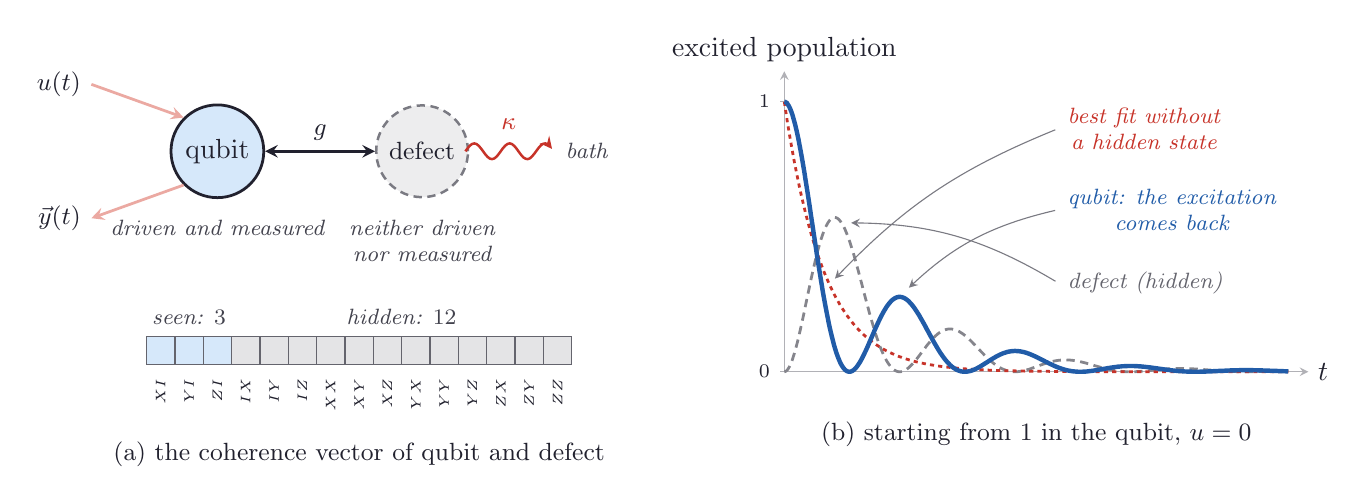
\begin{tikzpicture}[ink/.style={line width=0.9pt, ndInk}, faint/.style={line width=0.4pt, ndInk!35}, dashedink/.style={line width=0.5pt, ndInk!55, dash pattern=on 2.5pt off 2pt}, vec/.style={->, >=stealth, line width=1.2pt}, note/.style={font=\footnotesize\itshape, text=ndInk!85, align=center}, pointer/.style={->, >=stealth, line width=0.4pt, ndInk!60, shorten >=2pt, shorten <=1pt}, dot/.style={circle, fill=ndInk, inner sep=0pt, minimum size=3.4pt}, wash/.style={fill=ndSky, fill opacity=0.55}, every node/.style={text=ndInk}]
\definecolor{ndInk}{rgb}{0.13,0.13,0.18}
\definecolor{ndPaper}{rgb}{0.99,0.96,0.88}
\definecolor{ndSky}{rgb}{0.84,0.91,0.98}
\definecolor{ndRose}{rgb}{0.98,0.86,0.84}
\definecolor{ndBlue}{rgb}{0.13,0.36,0.66}
\definecolor{ndRed}{rgb}{0.78,0.20,0.16}
\definecolor{ndGold}{rgb}{0.88,0.62,0.10}
\definecolor{ndGreen}{rgb}{0.18,0.52,0.30}
\node[circle, draw=ndInk, line width=1.0pt, fill=ndSky, minimum size=1.05cm] (S) at (0,0.6) {qubit};
\node[circle, draw=ndInk!60, line width=0.9pt, dash pattern=on 3pt off 2pt, fill=ndInk!8, minimum size=1.05cm, font=\small] (T) at (2.6,0.6) {defect};
\draw[<->, >=stealth, line width=1.0pt, ndInk] (S) -- node[above, font=\small] {$g$} (T);
\draw[->, >=stealth, line width=0.9pt, ndRed] (3.150,0.600) -- (3.178,0.638) -- (3.206,0.671) -- (3.235,0.693) -- (3.263,0.700) -- (3.291,0.692) -- (3.319,0.670) -- (3.347,0.637) -- (3.376,0.598) -- (3.404,0.560) -- (3.432,0.528) -- (3.460,0.507) -- (3.488,0.500) -- (3.517,0.509) -- (3.545,0.531) -- (3.573,0.565) -- (3.601,0.603) -- (3.629,0.642) -- (3.658,0.673) -- (3.686,0.694) -- (3.714,0.700) -- (3.742,0.691) -- (3.771,0.667) -- (3.799,0.634) -- (3.827,0.595) -- (3.855,0.557) -- (3.883,0.525) -- (3.912,0.506) -- (3.940,0.500) -- (3.968,0.510) -- (3.996,0.534) -- (4.024,0.568) -- (4.053,0.607) -- (4.081,0.645) -- (4.109,0.676) -- (4.137,0.695) -- (4.165,0.700) -- (4.194,0.689) -- (4.222,0.665) -- (4.250,0.630);
\node[font=\small, text=ndRed, above] at (3.7,0.75) {$\kappa$};
\node[note, anchor=west] at (4.3,0.6) {bath};
\draw[->, >=stealth, line width=1.0pt, ndRose!70!ndRed] (-1.6,1.45) node[left, text=ndInk, font=\small] {$u(t)$} -- (S.north west);
\draw[->, >=stealth, line width=1.0pt, ndRose!70!ndRed] (S.south west) -- (-1.6,-0.25) node[left, text=ndInk, font=\small] {$\vec y(t)$};
\node[note, anchor=north] at (0,-0.15) {driven and measured};
\node[note, anchor=north] at (2.6,-0.15) {neither driven\\ nor measured};
\filldraw[fill=ndSky, draw=ndInk!70, line width=0.5pt] (-0.900,-1.75) rectangle (-0.540,-2.11);
\node[font=\tiny, rotate=90, anchor=east] at (-0.720,-2.16) {$XI$};
\filldraw[fill=ndSky, draw=ndInk!70, line width=0.5pt] (-0.540,-1.75) rectangle (-0.180,-2.11);
\node[font=\tiny, rotate=90, anchor=east] at (-0.360,-2.16) {$YI$};
\filldraw[fill=ndSky, draw=ndInk!70, line width=0.5pt] (-0.180,-1.75) rectangle (0.180,-2.11);
\node[font=\tiny, rotate=90, anchor=east] at (-0.000,-2.16) {$ZI$};
\filldraw[fill=ndInk!12, draw=ndInk!70, line width=0.5pt] (0.180,-1.75) rectangle (0.540,-2.11);
\node[font=\tiny, rotate=90, anchor=east] at (0.360,-2.16) {$IX$};
\filldraw[fill=ndInk!12, draw=ndInk!70, line width=0.5pt] (0.540,-1.75) rectangle (0.900,-2.11);
\node[font=\tiny, rotate=90, anchor=east] at (0.720,-2.16) {$IY$};
\filldraw[fill=ndInk!12, draw=ndInk!70, line width=0.5pt] (0.900,-1.75) rectangle (1.260,-2.11);
\node[font=\tiny, rotate=90, anchor=east] at (1.080,-2.16) {$IZ$};
\filldraw[fill=ndInk!12, draw=ndInk!70, line width=0.5pt] (1.260,-1.75) rectangle (1.620,-2.11);
\node[font=\tiny, rotate=90, anchor=east] at (1.440,-2.16) {$XX$};
\filldraw[fill=ndInk!12, draw=ndInk!70, line width=0.5pt] (1.620,-1.75) rectangle (1.980,-2.11);
\node[font=\tiny, rotate=90, anchor=east] at (1.800,-2.16) {$XY$};
\filldraw[fill=ndInk!12, draw=ndInk!70, line width=0.5pt] (1.980,-1.75) rectangle (2.340,-2.11);
\node[font=\tiny, rotate=90, anchor=east] at (2.160,-2.16) {$XZ$};
\filldraw[fill=ndInk!12, draw=ndInk!70, line width=0.5pt] (2.340,-1.75) rectangle (2.700,-2.11);
\node[font=\tiny, rotate=90, anchor=east] at (2.520,-2.16) {$YX$};
\filldraw[fill=ndInk!12, draw=ndInk!70, line width=0.5pt] (2.700,-1.75) rectangle (3.060,-2.11);
\node[font=\tiny, rotate=90, anchor=east] at (2.880,-2.16) {$YY$};
\filldraw[fill=ndInk!12, draw=ndInk!70, line width=0.5pt] (3.060,-1.75) rectangle (3.420,-2.11);
\node[font=\tiny, rotate=90, anchor=east] at (3.240,-2.16) {$YZ$};
\filldraw[fill=ndInk!12, draw=ndInk!70, line width=0.5pt] (3.420,-1.75) rectangle (3.780,-2.11);
\node[font=\tiny, rotate=90, anchor=east] at (3.600,-2.16) {$ZX$};
\filldraw[fill=ndInk!12, draw=ndInk!70, line width=0.5pt] (3.780,-1.75) rectangle (4.140,-2.11);
\node[font=\tiny, rotate=90, anchor=east] at (3.960,-2.16) {$ZY$};
\filldraw[fill=ndInk!12, draw=ndInk!70, line width=0.5pt] (4.140,-1.75) rectangle (4.500,-2.11);
\node[font=\tiny, rotate=90, anchor=east] at (4.320,-2.16) {$ZZ$};
\node[note, anchor=south] at (-0.360,-1.72) {seen: $3$};
\node[note, anchor=south] at (2.340,-1.72) {hidden: $12$};
\node[font=\small] at (1.8,-3.25) {(a) the coherence vector of qubit and defect};
\draw[faint, ->, >=stealth] (7.200,-2.200) -- (13.856,-2.200) node[right, text=ndInk] {$t$};
\draw[faint, ->, >=stealth] (7.200,-2.200) -- (7.200,1.616) node[above, text=ndInk] {excited population};
\draw[faint] (7.260,-2.200) -- (7.140,-2.200) node[left, font=\scriptsize, text=ndInk] {$0$};
\draw[faint] (7.260,1.229) -- (7.140,1.229) node[left, font=\scriptsize, text=ndInk] {$1$};
\draw[line width=1.0pt, ndInk!55, dash pattern=on 3pt off 2pt] (7.200,-2.200) -- (7.213,-2.197) -- (7.226,-2.189) -- (7.238,-2.177) -- (7.251,-2.159) -- (7.264,-2.137) -- (7.277,-2.110) -- (7.290,-2.079) -- (7.303,-2.045) -- (7.315,-2.006) -- (7.328,-1.965) -- (7.341,-1.920) -- (7.354,-1.872) -- (7.367,-1.822) -- (7.380,-1.770) -- (7.392,-1.715) -- (7.405,-1.659) -- (7.418,-1.601) -- (7.431,-1.542) -- (7.444,-1.482) -- (7.457,-1.421) -- (7.469,-1.360) -- (7.482,-1.298) -- (7.495,-1.236) -- (7.508,-1.175) -- (7.521,-1.114) -- (7.533,-1.054) -- (7.546,-0.995) -- (7.559,-0.937) -- (7.572,-0.880) -- (7.585,-0.825) -- (7.598,-0.771) -- (7.610,-0.719) -- (7.623,-0.670) -- (7.636,-0.622) -- (7.649,-0.577) -- (7.662,-0.534) -- (7.675,-0.494) -- (7.687,-0.457) -- (7.700,-0.422) -- (7.713,-0.390) -- (7.726,-0.361) -- (7.739,-0.335) -- (7.752,-0.312) -- (7.764,-0.293) -- (7.777,-0.276) -- (7.790,-0.262) -- (7.803,-0.252) -- (7.816,-0.245) -- (7.828,-0.241) -- (7.841,-0.240) -- (7.854,-0.242) -- (7.867,-0.247) -- (7.880,-0.255) -- (7.893,-0.266) -- (7.905,-0.280) -- (7.918,-0.297) -- (7.931,-0.316) -- (7.944,-0.338) -- (7.957,-0.363) -- (7.970,-0.390) -- (7.982,-0.419) -- (7.995,-0.451) -- (8.008,-0.484) -- (8.021,-0.520) -- (8.034,-0.557) -- (8.046,-0.596) -- (8.059,-0.637) -- (8.072,-0.679) -- (8.085,-0.722) -- (8.098,-0.767) -- (8.111,-0.813) -- (8.123,-0.859) -- (8.136,-0.906) -- (8.149,-0.954) -- (8.162,-1.003) -- (8.175,-1.052) -- (8.188,-1.101) -- (8.200,-1.150) -- (8.213,-1.199) -- (8.226,-1.248) -- (8.239,-1.296) -- (8.252,-1.344) -- (8.265,-1.392) -- (8.277,-1.439) -- (8.290,-1.485) -- (8.303,-1.530) -- (8.316,-1.575) -- (8.329,-1.618) -- (8.341,-1.660) -- (8.354,-1.701) -- (8.367,-1.741) -- (8.380,-1.780) -- (8.393,-1.816) -- (8.406,-1.852) -- (8.418,-1.886) -- (8.431,-1.918) -- (8.444,-1.948) -- (8.457,-1.977) -- (8.470,-2.004) -- (8.483,-2.030) -- (8.495,-2.053) -- (8.508,-2.075) -- (8.521,-2.095) -- (8.534,-2.113) -- (8.547,-2.130) -- (8.560,-2.145) -- (8.572,-2.157) -- (8.585,-2.169) -- (8.598,-2.178) -- (8.611,-2.186) -- (8.624,-2.192) -- (8.636,-2.196) -- (8.649,-2.199) -- (8.662,-2.200) -- (8.675,-2.200) -- (8.688,-2.198) -- (8.701,-2.195) -- (8.713,-2.190) -- (8.726,-2.184) -- (8.739,-2.177) -- (8.752,-2.169) -- (8.765,-2.160) -- (8.778,-2.149) -- (8.790,-2.138) -- (8.803,-2.126) -- (8.816,-2.113) -- (8.829,-2.099) -- (8.842,-2.085) -- (8.855,-2.070) -- (8.867,-2.054) -- (8.880,-2.039) -- (8.893,-2.022) -- (8.906,-2.006) -- (8.919,-1.989) -- (8.931,-1.972) -- (8.944,-1.955) -- (8.957,-1.938) -- (8.970,-1.921) -- (8.983,-1.904) -- (8.996,-1.887) -- (9.008,-1.870) -- (9.021,-1.854) -- (9.034,-1.838) -- (9.047,-1.823) -- (9.060,-1.808) -- (9.073,-1.793) -- (9.085,-1.779) -- (9.098,-1.766) -- (9.111,-1.753) -- (9.124,-1.741) -- (9.137,-1.730) -- (9.149,-1.719) -- (9.162,-1.710) -- (9.175,-1.700) -- (9.188,-1.692) -- (9.201,-1.685) -- (9.214,-1.678) -- (9.226,-1.673) -- (9.239,-1.668) -- (9.252,-1.664) -- (9.265,-1.661) -- (9.278,-1.658) -- (9.291,-1.657) -- (9.303,-1.656) -- (9.316,-1.657) -- (9.329,-1.658) -- (9.342,-1.660) -- (9.355,-1.663) -- (9.368,-1.666) -- (9.380,-1.671) -- (9.393,-1.676) -- (9.406,-1.682) -- (9.419,-1.688) -- (9.432,-1.696) -- (9.444,-1.704) -- (9.457,-1.712) -- (9.470,-1.721) -- (9.483,-1.731) -- (9.496,-1.741) -- (9.509,-1.752) -- (9.521,-1.763) -- (9.534,-1.775) -- (9.547,-1.787) -- (9.560,-1.799) -- (9.573,-1.812) -- (9.586,-1.824) -- (9.598,-1.838) -- (9.611,-1.851) -- (9.624,-1.864) -- (9.637,-1.878) -- (9.650,-1.891) -- (9.663,-1.905) -- (9.675,-1.918) -- (9.688,-1.932) -- (9.701,-1.946) -- (9.714,-1.959) -- (9.727,-1.972) -- (9.739,-1.985) -- (9.752,-1.998) -- (9.765,-2.011) -- (9.778,-2.023) -- (9.791,-2.035) -- (9.804,-2.047) -- (9.816,-2.059) -- (9.829,-2.070) -- (9.842,-2.080) -- (9.855,-2.091) -- (9.868,-2.101) -- (9.881,-2.110) -- (9.893,-2.119) -- (9.906,-2.128) -- (9.919,-2.136) -- (9.932,-2.144) -- (9.945,-2.151) -- (9.958,-2.158) -- (9.970,-2.164) -- (9.983,-2.169) -- (9.996,-2.175) -- (10.009,-2.179) -- (10.022,-2.184) -- (10.034,-2.187) -- (10.047,-2.190) -- (10.060,-2.193) -- (10.073,-2.195) -- (10.086,-2.197) -- (10.099,-2.199) -- (10.111,-2.199) -- (10.124,-2.200) -- (10.137,-2.200) -- (10.150,-2.200) -- (10.163,-2.199) -- (10.176,-2.198) -- (10.188,-2.196) -- (10.201,-2.194) -- (10.214,-2.192) -- (10.227,-2.190) -- (10.240,-2.187) -- (10.253,-2.184) -- (10.265,-2.180) -- (10.278,-2.177) -- (10.291,-2.173) -- (10.304,-2.169) -- (10.317,-2.165) -- (10.329,-2.161) -- (10.342,-2.156) -- (10.355,-2.152) -- (10.368,-2.147) -- (10.381,-2.143) -- (10.394,-2.138) -- (10.406,-2.133) -- (10.419,-2.129) -- (10.432,-2.124) -- (10.445,-2.119) -- (10.458,-2.114) -- (10.471,-2.110) -- (10.483,-2.105) -- (10.496,-2.101) -- (10.509,-2.097) -- (10.522,-2.092) -- (10.535,-2.088) -- (10.547,-2.084) -- (10.560,-2.081) -- (10.573,-2.077) -- (10.586,-2.074) -- (10.599,-2.071) -- (10.612,-2.068) -- (10.624,-2.065) -- (10.637,-2.062) -- (10.650,-2.060) -- (10.663,-2.058) -- (10.676,-2.056) -- (10.689,-2.054) -- (10.701,-2.053) -- (10.714,-2.052) -- (10.727,-2.051) -- (10.740,-2.050) -- (10.753,-2.049) -- (10.766,-2.049) -- (10.778,-2.049) -- (10.791,-2.050) -- (10.804,-2.050) -- (10.817,-2.051) -- (10.830,-2.052) -- (10.842,-2.053) -- (10.855,-2.054) -- (10.868,-2.056) -- (10.881,-2.058) -- (10.894,-2.060) -- (10.907,-2.062) -- (10.919,-2.064) -- (10.932,-2.067) -- (10.945,-2.069) -- (10.958,-2.072) -- (10.971,-2.075) -- (10.984,-2.078) -- (10.996,-2.081) -- (11.009,-2.084) -- (11.022,-2.088) -- (11.035,-2.091) -- (11.048,-2.095) -- (11.061,-2.098) -- (11.073,-2.102) -- (11.086,-2.106) -- (11.099,-2.110) -- (11.112,-2.113) -- (11.125,-2.117) -- (11.137,-2.121) -- (11.150,-2.125) -- (11.163,-2.128) -- (11.176,-2.132) -- (11.189,-2.136) -- (11.202,-2.139) -- (11.214,-2.143) -- (11.227,-2.147) -- (11.240,-2.150) -- (11.253,-2.153) -- (11.266,-2.157) -- (11.279,-2.160) -- (11.291,-2.163) -- (11.304,-2.166) -- (11.317,-2.169) -- (11.330,-2.172) -- (11.343,-2.174) -- (11.356,-2.177) -- (11.368,-2.179) -- (11.381,-2.182) -- (11.394,-2.184) -- (11.407,-2.186) -- (11.420,-2.188) -- (11.432,-2.189) -- (11.445,-2.191) -- (11.458,-2.193) -- (11.471,-2.194) -- (11.484,-2.195) -- (11.497,-2.196) -- (11.509,-2.197) -- (11.522,-2.198) -- (11.535,-2.199) -- (11.548,-2.199) -- (11.561,-2.200) -- (11.574,-2.200) -- (11.586,-2.200) -- (11.599,-2.200) -- (11.612,-2.200) -- (11.625,-2.200) -- (11.638,-2.199) -- (11.651,-2.199) -- (11.663,-2.199) -- (11.676,-2.198) -- (11.689,-2.197) -- (11.702,-2.197) -- (11.715,-2.196) -- (11.727,-2.195) -- (11.740,-2.194) -- (11.753,-2.193) -- (11.766,-2.192) -- (11.779,-2.191) -- (11.792,-2.189) -- (11.804,-2.188) -- (11.817,-2.187) -- (11.830,-2.186) -- (11.843,-2.184) -- (11.856,-2.183) -- (11.869,-2.182) -- (11.881,-2.181) -- (11.894,-2.179) -- (11.907,-2.178) -- (11.920,-2.177) -- (11.933,-2.175) -- (11.945,-2.174) -- (11.958,-2.173) -- (11.971,-2.172) -- (11.984,-2.170) -- (11.997,-2.169) -- (12.010,-2.168) -- (12.022,-2.167) -- (12.035,-2.166) -- (12.048,-2.165) -- (12.061,-2.164) -- (12.074,-2.163) -- (12.087,-2.163) -- (12.099,-2.162) -- (12.112,-2.161) -- (12.125,-2.161) -- (12.138,-2.160) -- (12.151,-2.160) -- (12.164,-2.159) -- (12.176,-2.159) -- (12.189,-2.159) -- (12.202,-2.158) -- (12.215,-2.158) -- (12.228,-2.158) -- (12.240,-2.158) -- (12.253,-2.158) -- (12.266,-2.158) -- (12.279,-2.159) -- (12.292,-2.159) -- (12.305,-2.159) -- (12.317,-2.159) -- (12.330,-2.160) -- (12.343,-2.160) -- (12.356,-2.161) -- (12.369,-2.161) -- (12.382,-2.162) -- (12.394,-2.163) -- (12.407,-2.164) -- (12.420,-2.164) -- (12.433,-2.165) -- (12.446,-2.166) -- (12.459,-2.167) -- (12.471,-2.168) -- (12.484,-2.169) -- (12.497,-2.170) -- (12.510,-2.171) -- (12.523,-2.172) -- (12.535,-2.173) -- (12.548,-2.174) -- (12.561,-2.175) -- (12.574,-2.176) -- (12.587,-2.177) -- (12.600,-2.178) -- (12.612,-2.179) -- (12.625,-2.180) -- (12.638,-2.181) -- (12.651,-2.182) -- (12.664,-2.183) -- (12.677,-2.184) -- (12.689,-2.185) -- (12.702,-2.186) -- (12.715,-2.187) -- (12.728,-2.188) -- (12.741,-2.189) -- (12.754,-2.189) -- (12.766,-2.190) -- (12.779,-2.191) -- (12.792,-2.192) -- (12.805,-2.193) -- (12.818,-2.193) -- (12.830,-2.194) -- (12.843,-2.195) -- (12.856,-2.195) -- (12.869,-2.196) -- (12.882,-2.196) -- (12.895,-2.197) -- (12.907,-2.197) -- (12.920,-2.198) -- (12.933,-2.198) -- (12.946,-2.199) -- (12.959,-2.199) -- (12.972,-2.199) -- (12.984,-2.199) -- (12.997,-2.200) -- (13.010,-2.200) -- (13.023,-2.200) -- (13.036,-2.200) -- (13.048,-2.200) -- (13.061,-2.200) -- (13.074,-2.200) -- (13.087,-2.200) -- (13.100,-2.200) -- (13.113,-2.200) -- (13.125,-2.200) -- (13.138,-2.199) -- (13.151,-2.199) -- (13.164,-2.199) -- (13.177,-2.199) -- (13.190,-2.199) -- (13.202,-2.198) -- (13.215,-2.198) -- (13.228,-2.198) -- (13.241,-2.197) -- (13.254,-2.197) -- (13.267,-2.197) -- (13.279,-2.197) -- (13.292,-2.196) -- (13.305,-2.196) -- (13.318,-2.195) -- (13.331,-2.195) -- (13.343,-2.195) -- (13.356,-2.194) -- (13.369,-2.194) -- (13.382,-2.194) -- (13.395,-2.193) -- (13.408,-2.193) -- (13.420,-2.193) -- (13.433,-2.192) -- (13.446,-2.192) -- (13.459,-2.192) -- (13.472,-2.191) -- (13.485,-2.191) -- (13.497,-2.191) -- (13.510,-2.190) -- (13.523,-2.190) -- (13.536,-2.190) -- (13.549,-2.190) -- (13.562,-2.190) -- (13.574,-2.189) -- (13.587,-2.189) -- (13.600,-2.189);
\draw[line width=1.0pt, ndRed, dash pattern=on 1.5pt off 1.5pt] (7.200,1.229) -- (7.213,1.143) -- (7.226,1.060) -- (7.238,0.978) -- (7.251,0.899) -- (7.264,0.822) -- (7.277,0.746) -- (7.290,0.673) -- (7.303,0.601) -- (7.315,0.531) -- (7.328,0.463) -- (7.341,0.397) -- (7.354,0.332) -- (7.367,0.269) -- (7.380,0.207) -- (7.392,0.147) -- (7.405,0.089) -- (7.418,0.031) -- (7.431,-0.024) -- (7.444,-0.079) -- (7.457,-0.131) -- (7.469,-0.183) -- (7.482,-0.233) -- (7.495,-0.282) -- (7.508,-0.330) -- (7.521,-0.377) -- (7.533,-0.422) -- (7.546,-0.467) -- (7.559,-0.510) -- (7.572,-0.552) -- (7.585,-0.593) -- (7.598,-0.633) -- (7.610,-0.672) -- (7.623,-0.711) -- (7.636,-0.748) -- (7.649,-0.784) -- (7.662,-0.819) -- (7.675,-0.854) -- (7.687,-0.887) -- (7.700,-0.920) -- (7.713,-0.952) -- (7.726,-0.983) -- (7.739,-1.013) -- (7.752,-1.043) -- (7.764,-1.072) -- (7.777,-1.100) -- (7.790,-1.128) -- (7.803,-1.154) -- (7.816,-1.180) -- (7.828,-1.206) -- (7.841,-1.231) -- (7.854,-1.255) -- (7.867,-1.278) -- (7.880,-1.301) -- (7.893,-1.324) -- (7.905,-1.346) -- (7.918,-1.367) -- (7.931,-1.388) -- (7.944,-1.408) -- (7.957,-1.428) -- (7.970,-1.447) -- (7.982,-1.466) -- (7.995,-1.484) -- (8.008,-1.502) -- (8.021,-1.519) -- (8.034,-1.536) -- (8.046,-1.553) -- (8.059,-1.569) -- (8.072,-1.585) -- (8.085,-1.600) -- (8.098,-1.615) -- (8.111,-1.630) -- (8.123,-1.644) -- (8.136,-1.658) -- (8.149,-1.671) -- (8.162,-1.685) -- (8.175,-1.697) -- (8.188,-1.710) -- (8.200,-1.722) -- (8.213,-1.734) -- (8.226,-1.746) -- (8.239,-1.757) -- (8.252,-1.768) -- (8.265,-1.779) -- (8.277,-1.789) -- (8.290,-1.800) -- (8.303,-1.810) -- (8.316,-1.819) -- (8.329,-1.829) -- (8.341,-1.838) -- (8.354,-1.847) -- (8.367,-1.856) -- (8.380,-1.865) -- (8.393,-1.873) -- (8.406,-1.881) -- (8.418,-1.889) -- (8.431,-1.897) -- (8.444,-1.904) -- (8.457,-1.912) -- (8.470,-1.919) -- (8.483,-1.926) -- (8.495,-1.933) -- (8.508,-1.939) -- (8.521,-1.946) -- (8.534,-1.952) -- (8.547,-1.958) -- (8.560,-1.964) -- (8.572,-1.970) -- (8.585,-1.976) -- (8.598,-1.982) -- (8.611,-1.987) -- (8.624,-1.992) -- (8.636,-1.998) -- (8.649,-2.003) -- (8.662,-2.008) -- (8.675,-2.012) -- (8.688,-2.017) -- (8.701,-2.022) -- (8.713,-2.026) -- (8.726,-2.030) -- (8.739,-2.035) -- (8.752,-2.039) -- (8.765,-2.043) -- (8.778,-2.047) -- (8.790,-2.051) -- (8.803,-2.054) -- (8.816,-2.058) -- (8.829,-2.061) -- (8.842,-2.065) -- (8.855,-2.068) -- (8.867,-2.072) -- (8.880,-2.075) -- (8.893,-2.078) -- (8.906,-2.081) -- (8.919,-2.084) -- (8.931,-2.087) -- (8.944,-2.090) -- (8.957,-2.092) -- (8.970,-2.095) -- (8.983,-2.098) -- (8.996,-2.100) -- (9.008,-2.103) -- (9.021,-2.105) -- (9.034,-2.108) -- (9.047,-2.110) -- (9.060,-2.112) -- (9.073,-2.114) -- (9.085,-2.116) -- (9.098,-2.118) -- (9.111,-2.121) -- (9.124,-2.123) -- (9.137,-2.124) -- (9.149,-2.126) -- (9.162,-2.128) -- (9.175,-2.130) -- (9.188,-2.132) -- (9.201,-2.133) -- (9.214,-2.135) -- (9.226,-2.137) -- (9.239,-2.138) -- (9.252,-2.140) -- (9.265,-2.141) -- (9.278,-2.143) -- (9.291,-2.144) -- (9.303,-2.146) -- (9.316,-2.147) -- (9.329,-2.148) -- (9.342,-2.150) -- (9.355,-2.151) -- (9.368,-2.152) -- (9.380,-2.153) -- (9.393,-2.154) -- (9.406,-2.156) -- (9.419,-2.157) -- (9.432,-2.158) -- (9.444,-2.159) -- (9.457,-2.160) -- (9.470,-2.161) -- (9.483,-2.162) -- (9.496,-2.163) -- (9.509,-2.164) -- (9.521,-2.165) -- (9.534,-2.165) -- (9.547,-2.166) -- (9.560,-2.167) -- (9.573,-2.168) -- (9.586,-2.169) -- (9.598,-2.170) -- (9.611,-2.170) -- (9.624,-2.171) -- (9.637,-2.172) -- (9.650,-2.172) -- (9.663,-2.173) -- (9.675,-2.174) -- (9.688,-2.175) -- (9.701,-2.175) -- (9.714,-2.176) -- (9.727,-2.176) -- (9.739,-2.177) -- (9.752,-2.178) -- (9.765,-2.178) -- (9.778,-2.179) -- (9.791,-2.179) -- (9.804,-2.180) -- (9.816,-2.180) -- (9.829,-2.181) -- (9.842,-2.181) -- (9.855,-2.182) -- (9.868,-2.182) -- (9.881,-2.183) -- (9.893,-2.183) -- (9.906,-2.183) -- (9.919,-2.184) -- (9.932,-2.184) -- (9.945,-2.185) -- (9.958,-2.185) -- (9.970,-2.185) -- (9.983,-2.186) -- (9.996,-2.186) -- (10.009,-2.186) -- (10.022,-2.187) -- (10.034,-2.187) -- (10.047,-2.187) -- (10.060,-2.188) -- (10.073,-2.188) -- (10.086,-2.188) -- (10.099,-2.189) -- (10.111,-2.189) -- (10.124,-2.189) -- (10.137,-2.189) -- (10.150,-2.190) -- (10.163,-2.190) -- (10.176,-2.190) -- (10.188,-2.190) -- (10.201,-2.191) -- (10.214,-2.191) -- (10.227,-2.191) -- (10.240,-2.191) -- (10.253,-2.192) -- (10.265,-2.192) -- (10.278,-2.192) -- (10.291,-2.192) -- (10.304,-2.192) -- (10.317,-2.193) -- (10.329,-2.193) -- (10.342,-2.193) -- (10.355,-2.193) -- (10.368,-2.193) -- (10.381,-2.193) -- (10.394,-2.194) -- (10.406,-2.194) -- (10.419,-2.194) -- (10.432,-2.194) -- (10.445,-2.194) -- (10.458,-2.194) -- (10.471,-2.195) -- (10.483,-2.195) -- (10.496,-2.195) -- (10.509,-2.195) -- (10.522,-2.195) -- (10.535,-2.195) -- (10.547,-2.195) -- (10.560,-2.195) -- (10.573,-2.196) -- (10.586,-2.196) -- (10.599,-2.196) -- (10.612,-2.196) -- (10.624,-2.196) -- (10.637,-2.196) -- (10.650,-2.196) -- (10.663,-2.196) -- (10.676,-2.196) -- (10.689,-2.196) -- (10.701,-2.197) -- (10.714,-2.197) -- (10.727,-2.197) -- (10.740,-2.197) -- (10.753,-2.197) -- (10.766,-2.197) -- (10.778,-2.197) -- (10.791,-2.197) -- (10.804,-2.197) -- (10.817,-2.197) -- (10.830,-2.197) -- (10.842,-2.197) -- (10.855,-2.197) -- (10.868,-2.198) -- (10.881,-2.198) -- (10.894,-2.198) -- (10.907,-2.198) -- (10.919,-2.198) -- (10.932,-2.198) -- (10.945,-2.198) -- (10.958,-2.198) -- (10.971,-2.198) -- (10.984,-2.198) -- (10.996,-2.198) -- (11.009,-2.198) -- (11.022,-2.198) -- (11.035,-2.198) -- (11.048,-2.198) -- (11.061,-2.198) -- (11.073,-2.198) -- (11.086,-2.198) -- (11.099,-2.198) -- (11.112,-2.198) -- (11.125,-2.198) -- (11.137,-2.199) -- (11.150,-2.199) -- (11.163,-2.199) -- (11.176,-2.199) -- (11.189,-2.199) -- (11.202,-2.199) -- (11.214,-2.199) -- (11.227,-2.199) -- (11.240,-2.199) -- (11.253,-2.199) -- (11.266,-2.199) -- (11.279,-2.199) -- (11.291,-2.199) -- (11.304,-2.199) -- (11.317,-2.199) -- (11.330,-2.199) -- (11.343,-2.199) -- (11.356,-2.199) -- (11.368,-2.199) -- (11.381,-2.199) -- (11.394,-2.199) -- (11.407,-2.199) -- (11.420,-2.199) -- (11.432,-2.199) -- (11.445,-2.199) -- (11.458,-2.199) -- (11.471,-2.199) -- (11.484,-2.199) -- (11.497,-2.199) -- (11.509,-2.199) -- (11.522,-2.199) -- (11.535,-2.199) -- (11.548,-2.199) -- (11.561,-2.199) -- (11.574,-2.199) -- (11.586,-2.199) -- (11.599,-2.199) -- (11.612,-2.199) -- (11.625,-2.199) -- (11.638,-2.199) -- (11.651,-2.199) -- (11.663,-2.199) -- (11.676,-2.199) -- (11.689,-2.200) -- (11.702,-2.200) -- (11.715,-2.200) -- (11.727,-2.200) -- (11.740,-2.200) -- (11.753,-2.200) -- (11.766,-2.200) -- (11.779,-2.200) -- (11.792,-2.200) -- (11.804,-2.200) -- (11.817,-2.200) -- (11.830,-2.200) -- (11.843,-2.200) -- (11.856,-2.200) -- (11.869,-2.200) -- (11.881,-2.200) -- (11.894,-2.200) -- (11.907,-2.200) -- (11.920,-2.200) -- (11.933,-2.200) -- (11.945,-2.200) -- (11.958,-2.200) -- (11.971,-2.200) -- (11.984,-2.200) -- (11.997,-2.200) -- (12.010,-2.200) -- (12.022,-2.200) -- (12.035,-2.200) -- (12.048,-2.200) -- (12.061,-2.200) -- (12.074,-2.200) -- (12.087,-2.200) -- (12.099,-2.200) -- (12.112,-2.200) -- (12.125,-2.200) -- (12.138,-2.200) -- (12.151,-2.200) -- (12.164,-2.200) -- (12.176,-2.200) -- (12.189,-2.200) -- (12.202,-2.200) -- (12.215,-2.200) -- (12.228,-2.200) -- (12.240,-2.200) -- (12.253,-2.200) -- (12.266,-2.200) -- (12.279,-2.200) -- (12.292,-2.200) -- (12.305,-2.200) -- (12.317,-2.200) -- (12.330,-2.200) -- (12.343,-2.200) -- (12.356,-2.200) -- (12.369,-2.200) -- (12.382,-2.200) -- (12.394,-2.200) -- (12.407,-2.200) -- (12.420,-2.200) -- (12.433,-2.200) -- (12.446,-2.200) -- (12.459,-2.200) -- (12.471,-2.200) -- (12.484,-2.200) -- (12.497,-2.200) -- (12.510,-2.200) -- (12.523,-2.200) -- (12.535,-2.200) -- (12.548,-2.200) -- (12.561,-2.200) -- (12.574,-2.200) -- (12.587,-2.200) -- (12.600,-2.200) -- (12.612,-2.200) -- (12.625,-2.200) -- (12.638,-2.200) -- (12.651,-2.200) -- (12.664,-2.200) -- (12.677,-2.200) -- (12.689,-2.200) -- (12.702,-2.200) -- (12.715,-2.200) -- (12.728,-2.200) -- (12.741,-2.200) -- (12.754,-2.200) -- (12.766,-2.200) -- (12.779,-2.200) -- (12.792,-2.200) -- (12.805,-2.200) -- (12.818,-2.200) -- (12.830,-2.200) -- (12.843,-2.200) -- (12.856,-2.200) -- (12.869,-2.200) -- (12.882,-2.200) -- (12.895,-2.200) -- (12.907,-2.200) -- (12.920,-2.200) -- (12.933,-2.200) -- (12.946,-2.200) -- (12.959,-2.200) -- (12.972,-2.200) -- (12.984,-2.200) -- (12.997,-2.200) -- (13.010,-2.200) -- (13.023,-2.200) -- (13.036,-2.200) -- (13.048,-2.200) -- (13.061,-2.200) -- (13.074,-2.200) -- (13.087,-2.200) -- (13.100,-2.200) -- (13.113,-2.200) -- (13.125,-2.200) -- (13.138,-2.200) -- (13.151,-2.200) -- (13.164,-2.200) -- (13.177,-2.200) -- (13.190,-2.200) -- (13.202,-2.200) -- (13.215,-2.200) -- (13.228,-2.200) -- (13.241,-2.200) -- (13.254,-2.200) -- (13.267,-2.200) -- (13.279,-2.200) -- (13.292,-2.200) -- (13.305,-2.200) -- (13.318,-2.200) -- (13.331,-2.200) -- (13.343,-2.200) -- (13.356,-2.200) -- (13.369,-2.200) -- (13.382,-2.200) -- (13.395,-2.200) -- (13.408,-2.200) -- (13.420,-2.200) -- (13.433,-2.200) -- (13.446,-2.200) -- (13.459,-2.200) -- (13.472,-2.200) -- (13.485,-2.200) -- (13.497,-2.200) -- (13.510,-2.200) -- (13.523,-2.200) -- (13.536,-2.200) -- (13.549,-2.200) -- (13.562,-2.200) -- (13.574,-2.200) -- (13.587,-2.200) -- (13.600,-2.200);
\draw[line width=1.6pt, ndBlue] (7.200,1.229) -- (7.213,1.226) -- (7.226,1.218) -- (7.238,1.205) -- (7.251,1.186) -- (7.264,1.163) -- (7.277,1.134) -- (7.290,1.101) -- (7.303,1.064) -- (7.315,1.021) -- (7.328,0.975) -- (7.341,0.925) -- (7.354,0.870) -- (7.367,0.812) -- (7.380,0.751) -- (7.392,0.686) -- (7.405,0.618) -- (7.418,0.547) -- (7.431,0.474) -- (7.444,0.398) -- (7.457,0.321) -- (7.469,0.241) -- (7.482,0.160) -- (7.495,0.078) -- (7.508,-0.006) -- (7.521,-0.091) -- (7.533,-0.176) -- (7.546,-0.261) -- (7.559,-0.347) -- (7.572,-0.433) -- (7.585,-0.519) -- (7.598,-0.604) -- (7.610,-0.688) -- (7.623,-0.771) -- (7.636,-0.854) -- (7.649,-0.935) -- (7.662,-1.015) -- (7.675,-1.093) -- (7.687,-1.169) -- (7.700,-1.243) -- (7.713,-1.315) -- (7.726,-1.385) -- (7.739,-1.452) -- (7.752,-1.517) -- (7.764,-1.580) -- (7.777,-1.639) -- (7.790,-1.696) -- (7.803,-1.750) -- (7.816,-1.801) -- (7.828,-1.849) -- (7.841,-1.894) -- (7.854,-1.936) -- (7.867,-1.975) -- (7.880,-2.011) -- (7.893,-2.043) -- (7.905,-2.072) -- (7.918,-2.099) -- (7.931,-2.122) -- (7.944,-2.142) -- (7.957,-2.159) -- (7.970,-2.173) -- (7.982,-2.184) -- (7.995,-2.192) -- (8.008,-2.197) -- (8.021,-2.200) -- (8.034,-2.200) -- (8.046,-2.197) -- (8.059,-2.192) -- (8.072,-2.184) -- (8.085,-2.175) -- (8.098,-2.163) -- (8.111,-2.149) -- (8.123,-2.133) -- (8.136,-2.115) -- (8.149,-2.096) -- (8.162,-2.075) -- (8.175,-2.052) -- (8.188,-2.028) -- (8.200,-2.003) -- (8.213,-1.977) -- (8.226,-1.950) -- (8.239,-1.923) -- (8.252,-1.894) -- (8.265,-1.865) -- (8.277,-1.836) -- (8.290,-1.806) -- (8.303,-1.776) -- (8.316,-1.747) -- (8.329,-1.717) -- (8.341,-1.687) -- (8.354,-1.658) -- (8.367,-1.629) -- (8.380,-1.600) -- (8.393,-1.572) -- (8.406,-1.545) -- (8.418,-1.519) -- (8.431,-1.493) -- (8.444,-1.469) -- (8.457,-1.445) -- (8.470,-1.423) -- (8.483,-1.402) -- (8.495,-1.381) -- (8.508,-1.363) -- (8.521,-1.345) -- (8.534,-1.329) -- (8.547,-1.314) -- (8.560,-1.301) -- (8.572,-1.289) -- (8.585,-1.279) -- (8.598,-1.270) -- (8.611,-1.263) -- (8.624,-1.257) -- (8.636,-1.253) -- (8.649,-1.250) -- (8.662,-1.249) -- (8.675,-1.250) -- (8.688,-1.251) -- (8.701,-1.255) -- (8.713,-1.259) -- (8.726,-1.265) -- (8.739,-1.273) -- (8.752,-1.282) -- (8.765,-1.292) -- (8.778,-1.303) -- (8.790,-1.316) -- (8.803,-1.329) -- (8.816,-1.344) -- (8.829,-1.360) -- (8.842,-1.377) -- (8.855,-1.395) -- (8.867,-1.413) -- (8.880,-1.432) -- (8.893,-1.453) -- (8.906,-1.473) -- (8.919,-1.495) -- (8.931,-1.517) -- (8.944,-1.539) -- (8.957,-1.562) -- (8.970,-1.585) -- (8.983,-1.608) -- (8.996,-1.632) -- (9.008,-1.656) -- (9.021,-1.679) -- (9.034,-1.703) -- (9.047,-1.727) -- (9.060,-1.751) -- (9.073,-1.774) -- (9.085,-1.797) -- (9.098,-1.820) -- (9.111,-1.843) -- (9.124,-1.865) -- (9.137,-1.887) -- (9.149,-1.908) -- (9.162,-1.929) -- (9.175,-1.949) -- (9.188,-1.969) -- (9.201,-1.987) -- (9.214,-2.006) -- (9.226,-2.023) -- (9.239,-2.040) -- (9.252,-2.056) -- (9.265,-2.071) -- (9.278,-2.086) -- (9.291,-2.099) -- (9.303,-2.112) -- (9.316,-2.124) -- (9.329,-2.135) -- (9.342,-2.145) -- (9.355,-2.154) -- (9.368,-2.162) -- (9.380,-2.170) -- (9.393,-2.177) -- (9.406,-2.182) -- (9.419,-2.187) -- (9.432,-2.191) -- (9.444,-2.195) -- (9.457,-2.197) -- (9.470,-2.199) -- (9.483,-2.200) -- (9.496,-2.200) -- (9.509,-2.199) -- (9.521,-2.198) -- (9.534,-2.196) -- (9.547,-2.194) -- (9.560,-2.191) -- (9.573,-2.187) -- (9.586,-2.183) -- (9.598,-2.178) -- (9.611,-2.173) -- (9.624,-2.167) -- (9.637,-2.161) -- (9.650,-2.154) -- (9.663,-2.147) -- (9.675,-2.140) -- (9.688,-2.133) -- (9.701,-2.125) -- (9.714,-2.117) -- (9.727,-2.109) -- (9.739,-2.101) -- (9.752,-2.093) -- (9.765,-2.085) -- (9.778,-2.077) -- (9.791,-2.068) -- (9.804,-2.060) -- (9.816,-2.052) -- (9.829,-2.044) -- (9.842,-2.036) -- (9.855,-2.028) -- (9.868,-2.021) -- (9.881,-2.013) -- (9.893,-2.006) -- (9.906,-1.999) -- (9.919,-1.993) -- (9.932,-1.986) -- (9.945,-1.980) -- (9.958,-1.975) -- (9.970,-1.969) -- (9.983,-1.964) -- (9.996,-1.960) -- (10.009,-1.956) -- (10.022,-1.952) -- (10.034,-1.948) -- (10.047,-1.945) -- (10.060,-1.943) -- (10.073,-1.941) -- (10.086,-1.939) -- (10.099,-1.938) -- (10.111,-1.937) -- (10.124,-1.936) -- (10.137,-1.936) -- (10.150,-1.937) -- (10.163,-1.938) -- (10.176,-1.939) -- (10.188,-1.940) -- (10.201,-1.942) -- (10.214,-1.945) -- (10.227,-1.947) -- (10.240,-1.950) -- (10.253,-1.954) -- (10.265,-1.957) -- (10.278,-1.961) -- (10.291,-1.966) -- (10.304,-1.970) -- (10.317,-1.975) -- (10.329,-1.980) -- (10.342,-1.986) -- (10.355,-1.991) -- (10.368,-1.997) -- (10.381,-2.003) -- (10.394,-2.009) -- (10.406,-2.015) -- (10.419,-2.021) -- (10.432,-2.028) -- (10.445,-2.034) -- (10.458,-2.041) -- (10.471,-2.047) -- (10.483,-2.054) -- (10.496,-2.060) -- (10.509,-2.067) -- (10.522,-2.074) -- (10.535,-2.080) -- (10.547,-2.086) -- (10.560,-2.093) -- (10.573,-2.099) -- (10.586,-2.105) -- (10.599,-2.111) -- (10.612,-2.117) -- (10.624,-2.123) -- (10.637,-2.129) -- (10.650,-2.134) -- (10.663,-2.140) -- (10.676,-2.145) -- (10.689,-2.150) -- (10.701,-2.154) -- (10.714,-2.159) -- (10.727,-2.163) -- (10.740,-2.167) -- (10.753,-2.171) -- (10.766,-2.175) -- (10.778,-2.178) -- (10.791,-2.181) -- (10.804,-2.184) -- (10.817,-2.187) -- (10.830,-2.189) -- (10.842,-2.191) -- (10.855,-2.193) -- (10.868,-2.195) -- (10.881,-2.196) -- (10.894,-2.197) -- (10.907,-2.198) -- (10.919,-2.199) -- (10.932,-2.200) -- (10.945,-2.200) -- (10.958,-2.200) -- (10.971,-2.200) -- (10.984,-2.200) -- (10.996,-2.199) -- (11.009,-2.198) -- (11.022,-2.198) -- (11.035,-2.197) -- (11.048,-2.196) -- (11.061,-2.194) -- (11.073,-2.193) -- (11.086,-2.191) -- (11.099,-2.190) -- (11.112,-2.188) -- (11.125,-2.186) -- (11.137,-2.184) -- (11.150,-2.182) -- (11.163,-2.180) -- (11.176,-2.178) -- (11.189,-2.176) -- (11.202,-2.173) -- (11.214,-2.171) -- (11.227,-2.169) -- (11.240,-2.166) -- (11.253,-2.164) -- (11.266,-2.162) -- (11.279,-2.160) -- (11.291,-2.157) -- (11.304,-2.155) -- (11.317,-2.153) -- (11.330,-2.151) -- (11.343,-2.149) -- (11.356,-2.147) -- (11.368,-2.145) -- (11.381,-2.143) -- (11.394,-2.141) -- (11.407,-2.140) -- (11.420,-2.138) -- (11.432,-2.136) -- (11.445,-2.135) -- (11.458,-2.134) -- (11.471,-2.133) -- (11.484,-2.131) -- (11.497,-2.130) -- (11.509,-2.130) -- (11.522,-2.129) -- (11.535,-2.128) -- (11.548,-2.128) -- (11.561,-2.127) -- (11.574,-2.127) -- (11.586,-2.127) -- (11.599,-2.127) -- (11.612,-2.127) -- (11.625,-2.127) -- (11.638,-2.127) -- (11.651,-2.128) -- (11.663,-2.128) -- (11.676,-2.129) -- (11.689,-2.130) -- (11.702,-2.131) -- (11.715,-2.131) -- (11.727,-2.132) -- (11.740,-2.134) -- (11.753,-2.135) -- (11.766,-2.136) -- (11.779,-2.137) -- (11.792,-2.139) -- (11.804,-2.140) -- (11.817,-2.142) -- (11.830,-2.143) -- (11.843,-2.145) -- (11.856,-2.146) -- (11.869,-2.148) -- (11.881,-2.150) -- (11.894,-2.152) -- (11.907,-2.153) -- (11.920,-2.155) -- (11.933,-2.157) -- (11.945,-2.159) -- (11.958,-2.161) -- (11.971,-2.163) -- (11.984,-2.164) -- (11.997,-2.166) -- (12.010,-2.168) -- (12.022,-2.170) -- (12.035,-2.172) -- (12.048,-2.173) -- (12.061,-2.175) -- (12.074,-2.177) -- (12.087,-2.178) -- (12.099,-2.180) -- (12.112,-2.181) -- (12.125,-2.183) -- (12.138,-2.184) -- (12.151,-2.186) -- (12.164,-2.187) -- (12.176,-2.188) -- (12.189,-2.189) -- (12.202,-2.191) -- (12.215,-2.192) -- (12.228,-2.193) -- (12.240,-2.194) -- (12.253,-2.194) -- (12.266,-2.195) -- (12.279,-2.196) -- (12.292,-2.197) -- (12.305,-2.197) -- (12.317,-2.198) -- (12.330,-2.198) -- (12.343,-2.199) -- (12.356,-2.199) -- (12.369,-2.199) -- (12.382,-2.200) -- (12.394,-2.200) -- (12.407,-2.200) -- (12.420,-2.200) -- (12.433,-2.200) -- (12.446,-2.200) -- (12.459,-2.200) -- (12.471,-2.200) -- (12.484,-2.199) -- (12.497,-2.199) -- (12.510,-2.199) -- (12.523,-2.199) -- (12.535,-2.198) -- (12.548,-2.198) -- (12.561,-2.197) -- (12.574,-2.197) -- (12.587,-2.196) -- (12.600,-2.196) -- (12.612,-2.195) -- (12.625,-2.195) -- (12.638,-2.194) -- (12.651,-2.193) -- (12.664,-2.193) -- (12.677,-2.192) -- (12.689,-2.192) -- (12.702,-2.191) -- (12.715,-2.190) -- (12.728,-2.190) -- (12.741,-2.189) -- (12.754,-2.188) -- (12.766,-2.188) -- (12.779,-2.187) -- (12.792,-2.187) -- (12.805,-2.186) -- (12.818,-2.185) -- (12.830,-2.185) -- (12.843,-2.184) -- (12.856,-2.184) -- (12.869,-2.183) -- (12.882,-2.183) -- (12.895,-2.182) -- (12.907,-2.182) -- (12.920,-2.182) -- (12.933,-2.181) -- (12.946,-2.181) -- (12.959,-2.181) -- (12.972,-2.181) -- (12.984,-2.180) -- (12.997,-2.180) -- (13.010,-2.180) -- (13.023,-2.180) -- (13.036,-2.180) -- (13.048,-2.180) -- (13.061,-2.180) -- (13.074,-2.180) -- (13.087,-2.180) -- (13.100,-2.180) -- (13.113,-2.180) -- (13.125,-2.180) -- (13.138,-2.180) -- (13.151,-2.180) -- (13.164,-2.181) -- (13.177,-2.181) -- (13.190,-2.181) -- (13.202,-2.181) -- (13.215,-2.182) -- (13.228,-2.182) -- (13.241,-2.182) -- (13.254,-2.183) -- (13.267,-2.183) -- (13.279,-2.184) -- (13.292,-2.184) -- (13.305,-2.185) -- (13.318,-2.185) -- (13.331,-2.185) -- (13.343,-2.186) -- (13.356,-2.186) -- (13.369,-2.187) -- (13.382,-2.187) -- (13.395,-2.188) -- (13.408,-2.188) -- (13.420,-2.189) -- (13.433,-2.189) -- (13.446,-2.190) -- (13.459,-2.190) -- (13.472,-2.191) -- (13.485,-2.191) -- (13.497,-2.192) -- (13.510,-2.192) -- (13.523,-2.193) -- (13.536,-2.193) -- (13.549,-2.194) -- (13.562,-2.194) -- (13.574,-2.195) -- (13.587,-2.195) -- (13.600,-2.196);
\node[note, anchor=west, text=ndBlue] (r) at (10.674,-0.143) {qubit: the excitation\\ comes back};
\draw[pointer] (r.west) to[bend right=15] (8.731,-1.181);
\node[note, anchor=west, text=ndInk!70] (d) at (10.674,-1.069) {defect (hidden)};
\draw[pointer] (d.west) to[bend right=15] (7.978,-0.308);
\node[note, anchor=west, text=ndRed] (m) at (10.674,0.886) {best fit without\\ a hidden state};
\draw[pointer] (m.west) to[bend right=12] (7.794,-1.068);
\node[font=\small] at (10.400,-3.000) {(b) starting from $\ket1$ in the qubit, $u=0$};
\end{tikzpicture}
}\end{center}
\vspace{-1ex}{\small $15$ components: $3$ seen, $12$ \alert{hidden}. The qubit's population revives: memory in the hidden state. Observable through the qubit: $8$ of $16$ ($u=0$), $11$ with control.}}
\end{frame}

\begin{frame}\ft{Input--output equivalence and similarity}
\ona{Two systems are said to be I/O indistinguishable under an input $\vec{u}$ if it leads to the same output response. If this is true for all inputs in some class $\mathcal{U}$, then we say these two systems are indistinguishable under $\mathcal{U}$ and write $\Sigma \underrel{\mathcal{U}}{\equiv} \widehat{\Sigma}$. If $\mathcal{U}$ is the set of all inputs, the two systems are \emph{input--output equivalent}. This is related to similarity: $\Sigma$ is similar to $\widehat{\Sigma}$ if one can convert between the two under a change of variables $\vec{x} = \mathbf{T}\widehat{\vec{x}}$ with $\mathbf T\in\R^{n\times n}$ invertible, written $\Sigma \sim\widehat{\Sigma}$. In terms of the system matrices,}
\onp{Change of coordinates $\vec x=\mathbf T\widehat{\vec x}$ leaves the data unchanged:}
\begin{equation}\label{eq:ch04:similarity}
        \widehat{\mathbf A} = \mathbf{T}^{-1} \mathbf A \mathbf{T}, \qquad
        \widehat{\mathbf N}_j = \mathbf{T}^{-1} \mathbf{N}_j \mathbf{T}, \qquad
        \widehat{\vec{b}} = \mathbf{T}^{-1}\vec{b}, \qquad
        \widehat{\mathbf{C}}  = \mathbf{C} \mathbf{T}.
\end{equation}
\begin{thm}[Minimal realisations are unique up to similarity]\label{thm:ch04:similarity}
For minimal systems, i.e., having full-rank controllability and observability matrices, I/O equivalence implies and is implied by similarity: $\Sigma \equiv \widehat{\Sigma}  \iff \Sigma \sim \widehat{\Sigma}$. For bilinear systems see \citet{Sontag2009}; for linear systems \citet{Sontag1998}.
\end{thm}
\ona{This theorem is the reason why controllability and observability matter for identification: any algorithm that fits the data returns \emph{some} realisation, and Theorem~\ref{thm:ch04:similarity} says that all of them are related by a coordinate change, provided the true system was minimal. Section~\ref{sec:ch04:identifiability} shows how the coordinate change is eliminated in the quantum setting.}
\onp{Any data-fitting algorithm returns \emph{a} realisation; minimality says all of them differ only by $\mathbf T$.}
\end{frame}

\section{Controllability of closed systems}

\begin{frame}\ft{The Lie algebra rank condition}
\ona{For closed systems (\Chap~\ref{C.Closed}) the state is the propagator $U\in\Un[d]$, and the model $\dot U=-\imath(\Hdrift+\sum_k u_k\Hctrl)U$ is a right-invariant bilinear system on a compact Lie group. Linear rank conditions do not apply directly, since the state space is a manifold, but their role is played by the \emph{dynamical Lie algebra} $\mathfrak{g}=\Lie\{-\imath\Hdrift,-\imath\Hctrl[1],\dots,-\imath\Hctrl[m]\}$ (Definition~\ref{def:dla} in \Chap~\ref{C.Closed}). Note the analogy with \eqref{eq:ch04:BDS_reach_and_obs}: iterated products of the generators are replaced by iterated commutators. Figures~\ref{fig:ch02:lie} and~\ref{fig:ch02:closure} of \Chap~\ref{C.Closed} show both ingredients: a loop of two flows that fails to close, by a step in the direction of their bracket, and the dimension of the span of brackets growing level by level until it saturates.}
\onp{Closed system $\dot U=-\imath(\Hdrift+\sum_k u_k\Hctrl)U$; dynamical Lie algebra $\mathfrak g=\Lie\{-\imath\Hdrift,-\imath\Hctrl[1],\dots\}$: iterated \alert{commutators} instead of products.}
\begin{thm}[Jurdjevic--Sussmann]\label{thm:ch04:js}
Let the controls be piecewise constant and unbounded. The reachable set $\Reach$ from $\Id$ is the connected Lie subgroup $\ee^{\mathfrak g}$ of $\Un[d]$ with Lie algebra $\mathfrak g$. In particular, the system is \emph{operator controllable} ($\Reach=\SU[d]$ up to phase) if and only if $\mathfrak g\supseteq\liesu[d]$, i.e.\ $\dim\mathfrak g\ge d^2-1$ \citep{DAlessandro2021}.
\end{thm}
\ona{\begin{pf}[Sketch]
With piecewise-constant controls the propagator is a product of exponentials $\ee^{X_k t_k}$, $X_k=-\imath(\Hdrift+\sum_j u_j^{(k)}\Hctrl[j])\in\mathfrak g$, so $\Reach$ is contained in the group $G=\ee^{\mathfrak g}$ generated by $\mathfrak g$ and is a semigroup in $G$. The key facts are: (i) the identity $\ee^{sX}\ee^{sY}\ee^{-sX}\ee^{-sY}=\ee^{s^2[X,Y]+O(s^3)}$ shows that directions in $[\mathfrak g,\mathfrak g]$ are approximately reachable, so $\Reach$ has non-empty interior in $G$; (ii) on a \emph{compact} group, every one-parameter semigroup $\{\ee^{Xt}:t\ge0\}$ has $\ee^{-Xt}$ in its closure, so the closure of $\Reach$ is a closed subgroup of $G$ with non-empty interior, hence equals $G$; (iii) a semigroup with non-empty interior that is dense in a connected group is the whole group. For $\mathfrak g=\liesu[d]$ or $\lieu[d]$ one obtains all of $\SU[d]$ or $\Un[d]$.
\end{pf}
This is the theorem announced as Theorem~\ref{thm:js-preview} in \Chap~\ref{C.Closed}. For a single qubit, $\{-\imath\sigma_z,-\imath\sigma_x\}$ generates $\liesu[2]$ because $\comm{\sigma_z}{\sigma_x}=2\imath\sigma_y$; for two qubits, Exercise~\ref{exe:su4} asked you to verify that a $ZZ$ drift together with local $X$ and $Y$ controls generates $\liesu[4]$. The dimension of $\mathfrak g$ is computed numerically by repeatedly commuting and testing linear independence, exactly as in the snippet below. Pure-state controllability, i.e., reaching every unit vector rather than every unitary, is weaker; it holds iff the group $\ee^{\mathfrak g}$ acts transitively on the unit sphere, which happens for $\liesu[d]$ and also for $\mathfrak{sp}(d/2)$ \citep{DAlessandro2021}.}
\onp{\begin{itemize}
    \item Proof: commutators are approximately reachable ($\ee^{sX}\ee^{sY}\ee^{-sX}\ee^{-sY}\approx\ee^{s^2[X,Y]}$); compactness turns the reachable semigroup into a group.
    \item Qubit: $\comm{\sigma_z}{\sigma_x}=2\imath\sigma_y$ $\Rightarrow$ $\liesu[2]$. Two qubits: $ZZ$ drift $+$ local $X,Y$ $\Rightarrow$ $\liesu[4]$ (dimension 15).
    \item Pure-state controllability is weaker (transitivity on the sphere).
\end{itemize}}
\end{frame}

\begin{frame}[fragile]\ft{Computing the Lie closure and the observability matrix}
\ona{The abstract rank conditions become two short loops. The Lie closure repeatedly commutes the current generators and keeps the results that increase the rank of the (real) span; the observability matrix is a stack of $\mathbf C\mathbf A^k$. The script \texttt{code/ch04\_observability.py} implements both and reproduces the numbers quoted in this \chap{}.}
\ona{\lstinputlisting[style=python,firstline=65,lastline=95]{code/ch04_observability.py}}
\onp{\lstinputlisting[style=python,basicstyle=\ttfamily\tiny,numbers=none,firstline=75,lastline=95]{code/ch04_observability.py}}
\onp{Output: $\dim\Lie\{\imath Z,\imath X\}=3$, $\dim\Lie\{\imath ZZ,\imath X_1,\imath Y_1,\imath X_2,\imath Y_2\}=15$.}
\end{frame}

\begin{frame}\ft{Open systems: accessibility rather than controllability}
\ona{The identifiability of Markovian open quantum systems was also considered by \citet{Burgarth_2014}. They build on their previous work \citep{Burgarth_2012}, where they treat closed quantum systems as a black box that is known to be unitary and found that they are identifiable up to unitary equivalence if controllability is satisfied. In the open case, the unitary constraint is removed and dynamics are governed by a driven Lindblad equation $\dot \rho(t) = \Lind_0(\rho(t)) + \sum_{k} u_{k}(t) \Lind_{k}(\rho(t))$ with Lindblad super-operators $\Lind_k$. Because Markovian open systems are irreversible, operator controllability is not useful here, and instead one considers the concept of operator \emph{accessibility}, which states that all directions can be explored even when the dynamics are irreversible \citep{Dirr08}. By expressing the density matrix in an orthogonal Hermitian basis, they arrive at the affine LDS form $\dot{\vec x}=\mathbf A\vec x+\vec\beta$ with $ \mathbf{A} = \mathbf{A}_0 + \sum_{k} u_{k}(t)\mathbf{A}_k$ and $\vec \beta = \vec \beta_0 + \sum_{k} u_k(t)\vec\beta_k$. These define the generators of the system's Lie algebra as the set $\big\{\big(\begin{smallmatrix}\mathbf{A}_{k} & \vec\beta_k \\ \mathbf{0} & 0\end{smallmatrix}\big) \big\}_{k}$, and the system is accessible if this Lie algebra is the full algebra of affine maps}
\onp{Irreversible dynamics: replace controllability by \alert{accessibility} \citep{Dirr08,Burgarth_2014}. Affine generators $\big(\begin{smallmatrix}\mathbf A_k&\vec\beta_k\\ \mathbf 0&0\end{smallmatrix}\big)$ must generate}
\begin{equation}\label{eq:ch04:affine_lie}
    \mathfrak{l}
= \left\{\,
\begin{pmatrix}
    \mathbf{X} & \vec{x} \\
    \mathbf{0} & 0
\end{pmatrix}
\,\middle|\,
\mathbf{X} \in \R^{n \times n},\;
\vec{x} \in \R^{n}
\,\right\}.
\end{equation}
\ona{When accessibility is satisfied, the authors show that this guarantees rank conditions which ensure the system is identifiable up to similarity transform. They further exhibit two valid Lindblad generators related by an admissible similarity transform, both of which remain Lindbladian but whose Kossakowski spectra differ, and a pure unitary generator for which the same similarity transform leads to a nonphysical Kossakowski spectrum. Hence, not all similarity transforms preserve the Lindblad structure, and additional physical constraints may restrict the set of admissible transformations. We return to this in Section~\ref{sec:ch04:identifiability}.}
\onp{\begin{itemize}
    \item Accessibility $\Rightarrow$ identifiable up to similarity.
    \item Similarity transforms need not preserve the Lindblad structure: a genuine ambiguity, resolved below by fixing the frame.
\end{itemize}}
\end{frame}

\begin{frame}\ft{Accessible, but not controllable}
\ona{Figure~\ref{fig:ch04:accessibility} shows the difference between accessibility and controllability for a single qubit. With dissipation, the controls can still steer the state in every direction, so that the set of reachable states has interior, but they cannot undo the dissipation. Dephasing is unital (\Chap~\ref{C.Open}), so the length of the Bloch vector, and with it the purity, can never increase: the reachable states stay inside the sphere through the initial state. Amplitude damping is not unital and moves the centre of the ball, so purer states become reachable, but only towards the ground state, which is the mechanism behind reset. In neither case can the controls reach every state, so controllability fails, while accessibility, which asks only for interior, holds.}
\ona{\begin{figure}[H]\centering
\resizebox{\linewidth}{!}{% Generated by code/needham.py -- do not edit by hand.
\definecolor{qocA}{rgb}{0.00,0.45,0.70}
\definecolor{qocB}{rgb}{0.90,0.60,0.00}
\definecolor{qocC}{rgb}{0.00,0.62,0.45}
\definecolor{qocD}{rgb}{0.80,0.40,0.00}
\definecolor{qocE}{rgb}{0.80,0.60,0.70}
\definecolor{qocF}{rgb}{0.35,0.70,0.90}
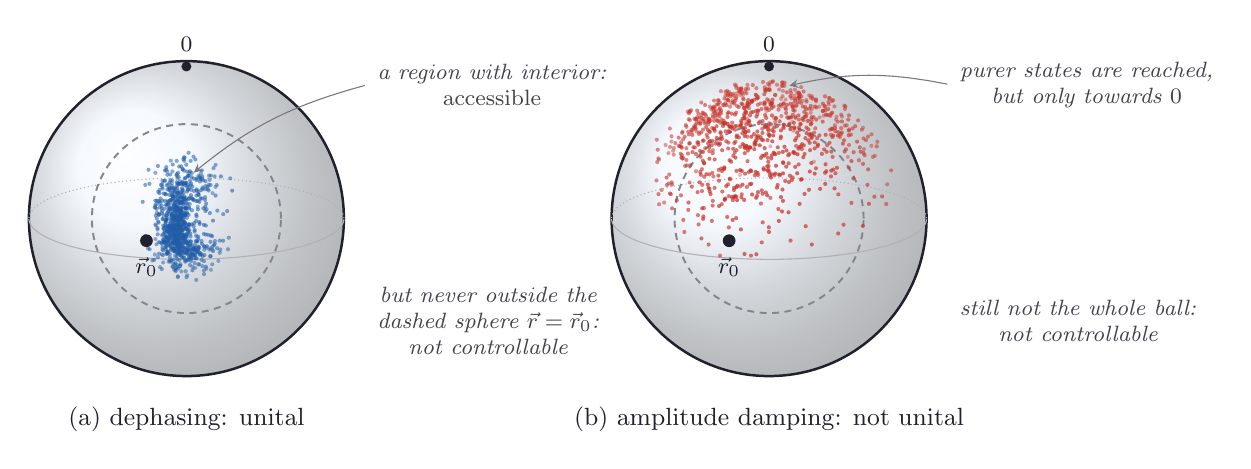
\begin{tikzpicture}[ink/.style={line width=0.9pt, ndInk}, faint/.style={line width=0.4pt, ndInk!35}, dashedink/.style={line width=0.5pt, ndInk!55, dash pattern=on 2.5pt off 2pt}, vec/.style={->, >=stealth, line width=1.2pt}, note/.style={font=\footnotesize\itshape, text=ndInk!85, align=center}, pointer/.style={->, >=stealth, line width=0.4pt, ndInk!60, shorten >=2pt, shorten <=1pt}, dot/.style={circle, fill=ndInk, inner sep=0pt, minimum size=3.4pt}, wash/.style={fill=ndSky, fill opacity=0.55}, every node/.style={text=ndInk}]
\definecolor{ndInk}{rgb}{0.13,0.13,0.18}
\definecolor{ndPaper}{rgb}{0.99,0.96,0.88}
\definecolor{ndSky}{rgb}{0.84,0.91,0.98}
\definecolor{ndRose}{rgb}{0.98,0.86,0.84}
\definecolor{ndBlue}{rgb}{0.13,0.36,0.66}
\definecolor{ndRed}{rgb}{0.78,0.20,0.16}
\definecolor{ndGold}{rgb}{0.88,0.62,0.10}
\definecolor{ndGreen}{rgb}{0.18,0.52,0.30}
\shade[ball color=ndSky!70!white, opacity=0.45] (0.000,0.000) circle (2.000);
\draw[ink] (0.000,0.000) circle (2.000);
\draw[faint] (1.813,-0.219) -- (1.834,-0.206) -- (1.854,-0.194) -- (1.873,-0.181) -- (1.891,-0.169) -- (1.907,-0.156) -- (1.923,-0.143) -- (1.936,-0.130) -- (1.949,-0.116) -- (1.960,-0.103) -- (1.970,-0.090) -- (1.978,-0.077) -- (1.985,-0.063) -- (1.991,-0.050) -- (1.995,-0.036) -- (1.998,-0.023) -- (2.000,-0.009);
\draw[faint] (-2.000,-0.005) -- (-1.999,-0.018) -- (-1.996,-0.032) -- (-1.992,-0.045) -- (-1.987,-0.059) -- (-1.981,-0.072) -- (-1.973,-0.085) -- (-1.963,-0.099) -- (-1.953,-0.112) -- (-1.941,-0.125) -- (-1.927,-0.138) -- (-1.913,-0.151) -- (-1.897,-0.164) -- (-1.879,-0.177) -- (-1.861,-0.190) -- (-1.841,-0.202) -- (-1.820,-0.215) -- (-1.798,-0.227) -- (-1.774,-0.239) -- (-1.749,-0.251) -- (-1.723,-0.263) -- (-1.696,-0.274) -- (-1.668,-0.286) -- (-1.638,-0.297) -- (-1.608,-0.308) -- (-1.576,-0.319) -- (-1.543,-0.329) -- (-1.509,-0.340) -- (-1.475,-0.350) -- (-1.439,-0.360) -- (-1.402,-0.369) -- (-1.364,-0.379) -- (-1.325,-0.388) -- (-1.286,-0.397) -- (-1.245,-0.405) -- (-1.204,-0.413) -- (-1.161,-0.421) -- (-1.118,-0.429) -- (-1.075,-0.437) -- (-1.030,-0.444) -- (-0.985,-0.451) -- (-0.939,-0.457) -- (-0.892,-0.463) -- (-0.845,-0.469) -- (-0.797,-0.475) -- (-0.749,-0.480) -- (-0.700,-0.485) -- (-0.651,-0.489) -- (-0.601,-0.494) -- (-0.551,-0.498) -- (-0.501,-0.501) -- (-0.450,-0.504) -- (-0.399,-0.507) -- (-0.347,-0.510) -- (-0.296,-0.512) -- (-0.244,-0.514) -- (-0.192,-0.515) -- (-0.140,-0.516) -- (-0.087,-0.517) -- (-0.035,-0.518) -- (0.017,-0.518) -- (0.070,-0.517) -- (0.122,-0.517) -- (0.174,-0.516) -- (0.226,-0.514) -- (0.278,-0.513) -- (0.330,-0.511) -- (0.382,-0.508) -- (0.433,-0.505) -- (0.484,-0.502) -- (0.534,-0.499) -- (0.585,-0.495) -- (0.635,-0.491) -- (0.684,-0.486) -- (0.733,-0.482) -- (0.781,-0.476) -- (0.829,-0.471) -- (0.877,-0.465) -- (0.923,-0.459) -- (0.970,-0.453) -- (1.015,-0.446) -- (1.060,-0.439) -- (1.104,-0.432) -- (1.147,-0.424) -- (1.190,-0.416) -- (1.231,-0.408) -- (1.272,-0.399) -- (1.312,-0.391) -- (1.351,-0.382) -- (1.389,-0.372) -- (1.427,-0.363) -- (1.463,-0.353) -- (1.498,-0.343) -- (1.532,-0.333) -- (1.565,-0.322) -- (1.597,-0.312) -- (1.628,-0.301) -- (1.658,-0.289) -- (1.687,-0.278) -- (1.714,-0.267) -- (1.741,-0.255) -- (1.766,-0.243) -- (1.790,-0.231) -- (1.813,-0.219);
\draw[faint, densely dotted] (2.000,0.005) -- (1.999,0.018) -- (1.996,0.032) -- (1.992,0.045) -- (1.987,0.059) -- (1.981,0.072) -- (1.973,0.085) -- (1.963,0.099) -- (1.953,0.112) -- (1.941,0.125) -- (1.927,0.138) -- (1.913,0.151) -- (1.897,0.164) -- (1.879,0.177) -- (1.861,0.190) -- (1.841,0.202) -- (1.820,0.215) -- (1.798,0.227) -- (1.774,0.239) -- (1.749,0.251) -- (1.723,0.263) -- (1.696,0.274) -- (1.668,0.286) -- (1.638,0.297) -- (1.608,0.308) -- (1.576,0.319) -- (1.543,0.329) -- (1.509,0.340) -- (1.475,0.350) -- (1.439,0.360) -- (1.402,0.369) -- (1.364,0.379) -- (1.325,0.388) -- (1.286,0.397) -- (1.245,0.405) -- (1.204,0.413) -- (1.161,0.421) -- (1.118,0.429) -- (1.075,0.437) -- (1.030,0.444) -- (0.985,0.451) -- (0.939,0.457) -- (0.892,0.463) -- (0.845,0.469) -- (0.797,0.475) -- (0.749,0.480) -- (0.700,0.485) -- (0.651,0.489) -- (0.601,0.494) -- (0.551,0.498) -- (0.501,0.501) -- (0.450,0.504) -- (0.399,0.507) -- (0.347,0.510) -- (0.296,0.512) -- (0.244,0.514) -- (0.192,0.515) -- (0.140,0.516) -- (0.087,0.517) -- (0.035,0.518) -- (-0.017,0.518) -- (-0.070,0.517) -- (-0.122,0.517) -- (-0.174,0.516) -- (-0.226,0.514) -- (-0.278,0.513) -- (-0.330,0.511) -- (-0.382,0.508) -- (-0.433,0.505) -- (-0.484,0.502) -- (-0.534,0.499) -- (-0.585,0.495) -- (-0.635,0.491) -- (-0.684,0.486) -- (-0.733,0.482) -- (-0.781,0.476) -- (-0.829,0.471) -- (-0.877,0.465) -- (-0.923,0.459) -- (-0.970,0.453) -- (-1.015,0.446) -- (-1.060,0.439) -- (-1.104,0.432) -- (-1.147,0.424) -- (-1.190,0.416) -- (-1.231,0.408) -- (-1.272,0.399) -- (-1.312,0.391) -- (-1.351,0.382) -- (-1.389,0.372) -- (-1.427,0.363) -- (-1.463,0.353) -- (-1.498,0.343) -- (-1.532,0.333) -- (-1.565,0.322) -- (-1.597,0.312) -- (-1.628,0.301) -- (-1.658,0.289) -- (-1.687,0.278) -- (-1.714,0.267) -- (-1.741,0.255) -- (-1.766,0.243) -- (-1.790,0.231) -- (-1.813,0.219) -- (-1.834,0.206) -- (-1.854,0.194) -- (-1.873,0.181) -- (-1.891,0.169) -- (-1.907,0.156) -- (-1.923,0.143) -- (-1.936,0.130) -- (-1.949,0.116) -- (-1.960,0.103) -- (-1.970,0.090) -- (-1.978,0.077) -- (-1.985,0.063) -- (-1.991,0.050) -- (-1.995,0.036) -- (-1.998,0.023) -- (-2.000,0.009);
\draw[dashedink, line width=0.7pt] (0.000,0.000) circle (1.200);
\fill[ndBlue, opacity=0.45] (0.311,-0.650) circle (0.75pt);
\fill[ndBlue, opacity=0.45] (-0.311,-0.456) circle (0.75pt);
\fill[ndBlue, opacity=0.45] (0.144,0.151) circle (0.75pt);
\fill[ndBlue, opacity=0.45] (0.245,-0.203) circle (0.75pt);
\fill[ndBlue, opacity=0.45] (0.332,-0.395) circle (0.75pt);
\fill[ndBlue, opacity=0.46] (-0.175,-0.304) circle (0.75pt);
\fill[ndBlue, opacity=0.46] (0.038,-0.148) circle (0.75pt);
\fill[ndBlue, opacity=0.46] (0.112,-0.465) circle (0.75pt);
\fill[ndBlue, opacity=0.46] (0.406,-0.537) circle (0.75pt);
\fill[ndBlue, opacity=0.46] (0.370,0.402) circle (0.75pt);
\fill[ndBlue, opacity=0.46] (-0.268,-0.173) circle (0.75pt);
\fill[ndBlue, opacity=0.47] (-0.096,-0.411) circle (0.75pt);
\fill[ndBlue, opacity=0.47] (0.129,-0.422) circle (0.75pt);
\fill[ndBlue, opacity=0.47] (0.195,-0.455) circle (0.75pt);
\fill[ndBlue, opacity=0.47] (-0.030,-0.388) circle (0.75pt);
\fill[ndBlue, opacity=0.47] (0.333,0.323) circle (0.75pt);
\fill[ndBlue, opacity=0.47] (-0.329,-0.305) circle (0.75pt);
\fill[ndBlue, opacity=0.47] (-0.109,-0.743) circle (0.75pt);
\fill[ndBlue, opacity=0.47] (-0.111,-0.370) circle (0.75pt);
\fill[ndBlue, opacity=0.47] (0.108,-0.388) circle (0.75pt);
\fill[ndBlue, opacity=0.48] (-0.157,-0.649) circle (0.75pt);
\fill[ndBlue, opacity=0.48] (-0.385,-0.087) circle (0.75pt);
\fill[ndBlue, opacity=0.48] (0.253,-0.636) circle (0.75pt);
\fill[ndBlue, opacity=0.48] (-0.145,-0.586) circle (0.75pt);
\fill[ndBlue, opacity=0.48] (-0.393,-0.259) circle (0.75pt);
\fill[ndBlue, opacity=0.48] (-0.056,-0.420) circle (0.75pt);
\fill[ndBlue, opacity=0.48] (-0.100,-0.387) circle (0.75pt);
\fill[ndBlue, opacity=0.48] (-0.090,-0.388) circle (0.75pt);
\fill[ndBlue, opacity=0.48] (0.001,-0.532) circle (0.75pt);
\fill[ndBlue, opacity=0.48] (-0.211,-0.350) circle (0.75pt);
\fill[ndBlue, opacity=0.48] (-0.209,-0.451) circle (0.75pt);
\fill[ndBlue, opacity=0.48] (0.206,0.397) circle (0.75pt);
\fill[ndBlue, opacity=0.48] (-0.063,-0.671) circle (0.75pt);
\fill[ndBlue, opacity=0.49] (-0.011,-0.428) circle (0.75pt);
\fill[ndBlue, opacity=0.49] (-0.107,-0.733) circle (0.75pt);
\fill[ndBlue, opacity=0.49] (-0.121,-0.585) circle (0.75pt);
\fill[ndBlue, opacity=0.49] (0.118,-0.368) circle (0.75pt);
\fill[ndBlue, opacity=0.49] (0.165,-0.582) circle (0.75pt);
\fill[ndBlue, opacity=0.49] (0.227,-0.396) circle (0.75pt);
\fill[ndBlue, opacity=0.49] (0.214,0.486) circle (0.75pt);
\fill[ndBlue, opacity=0.49] (-0.253,-0.332) circle (0.75pt);
\fill[ndBlue, opacity=0.49] (-0.295,-0.557) circle (0.75pt);
\fill[ndBlue, opacity=0.49] (-0.077,-0.600) circle (0.75pt);
\fill[ndBlue, opacity=0.49] (0.010,-0.721) circle (0.75pt);
\fill[ndBlue, opacity=0.49] (0.155,-0.363) circle (0.75pt);
\fill[ndBlue, opacity=0.49] (-0.105,-0.270) circle (0.75pt);
\fill[ndBlue, opacity=0.49] (0.149,-0.580) circle (0.75pt);
\fill[ndBlue, opacity=0.49] (-0.395,0.581) circle (0.75pt);
\fill[ndBlue, opacity=0.49] (0.111,-0.626) circle (0.75pt);
\fill[ndBlue, opacity=0.49] (-0.242,-0.414) circle (0.75pt);
\fill[ndBlue, opacity=0.49] (-0.298,-0.465) circle (0.75pt);
\fill[ndBlue, opacity=0.49] (0.016,-0.379) circle (0.75pt);
\fill[ndBlue, opacity=0.49] (-0.262,-0.360) circle (0.75pt);
\fill[ndBlue, opacity=0.49] (-0.028,0.779) circle (0.75pt);
\fill[ndBlue, opacity=0.49] (-0.244,0.600) circle (0.75pt);
\fill[ndBlue, opacity=0.49] (0.001,-0.745) circle (0.75pt);
\fill[ndBlue, opacity=0.49] (-0.401,-0.456) circle (0.75pt);
\fill[ndBlue, opacity=0.50] (-0.089,-0.527) circle (0.75pt);
\fill[ndBlue, opacity=0.50] (0.063,-0.444) circle (0.75pt);
\fill[ndBlue, opacity=0.50] (0.125,-0.779) circle (0.75pt);
\fill[ndBlue, opacity=0.50] (-0.292,-0.259) circle (0.75pt);
\fill[ndBlue, opacity=0.50] (-0.279,-0.177) circle (0.75pt);
\fill[ndBlue, opacity=0.50] (-0.307,-0.299) circle (0.75pt);
\fill[ndBlue, opacity=0.50] (-0.335,-0.617) circle (0.75pt);
\fill[ndBlue, opacity=0.50] (0.352,-0.337) circle (0.75pt);
\fill[ndBlue, opacity=0.50] (0.070,0.579) circle (0.75pt);
\fill[ndBlue, opacity=0.50] (0.023,-0.526) circle (0.75pt);
\fill[ndBlue, opacity=0.50] (-0.020,0.510) circle (0.75pt);
\fill[ndBlue, opacity=0.50] (-0.178,0.599) circle (0.75pt);
\fill[ndBlue, opacity=0.50] (-0.098,-0.369) circle (0.75pt);
\fill[ndBlue, opacity=0.50] (0.328,-0.581) circle (0.75pt);
\fill[ndBlue, opacity=0.50] (-0.180,0.485) circle (0.75pt);
\fill[ndBlue, opacity=0.50] (0.016,-0.397) circle (0.75pt);
\fill[ndBlue, opacity=0.50] (-0.380,-0.326) circle (0.75pt);
\fill[ndBlue, opacity=0.50] (-0.186,0.450) circle (0.75pt);
\fill[ndBlue, opacity=0.50] (-0.057,-0.494) circle (0.75pt);
\fill[ndBlue, opacity=0.50] (-0.304,-0.361) circle (0.75pt);
\fill[ndBlue, opacity=0.50] (0.183,0.576) circle (0.75pt);
\fill[ndBlue, opacity=0.50] (-0.092,-0.346) circle (0.75pt);
\fill[ndBlue, opacity=0.50] (-0.366,-0.139) circle (0.75pt);
\fill[ndBlue, opacity=0.51] (-0.178,-0.606) circle (0.75pt);
\fill[ndBlue, opacity=0.51] (0.192,-0.524) circle (0.75pt);
\fill[ndBlue, opacity=0.51] (-0.194,-0.362) circle (0.75pt);
\fill[ndBlue, opacity=0.51] (0.180,0.516) circle (0.75pt);
\fill[ndBlue, opacity=0.51] (-0.136,-0.667) circle (0.75pt);
\fill[ndBlue, opacity=0.51] (0.103,-0.391) circle (0.75pt);
\fill[ndBlue, opacity=0.51] (-0.304,-0.391) circle (0.75pt);
\fill[ndBlue, opacity=0.51] (0.014,-0.410) circle (0.75pt);
\fill[ndBlue, opacity=0.51] (-0.047,0.629) circle (0.75pt);
\fill[ndBlue, opacity=0.51] (0.053,-0.511) circle (0.75pt);
\fill[ndBlue, opacity=0.51] (0.339,-0.413) circle (0.75pt);
\fill[ndBlue, opacity=0.51] (-0.466,-0.390) circle (0.75pt);
\fill[ndBlue, opacity=0.51] (-0.271,0.480) circle (0.75pt);
\fill[ndBlue, opacity=0.51] (0.090,-0.503) circle (0.75pt);
\fill[ndBlue, opacity=0.51] (-0.114,0.515) circle (0.75pt);
\fill[ndBlue, opacity=0.51] (-0.083,-0.601) circle (0.75pt);
\fill[ndBlue, opacity=0.51] (-0.100,-0.398) circle (0.75pt);
\fill[ndBlue, opacity=0.51] (-0.051,-0.349) circle (0.75pt);
\fill[ndBlue, opacity=0.51] (0.363,-0.284) circle (0.75pt);
\fill[ndBlue, opacity=0.51] (0.051,-0.348) circle (0.75pt);
\fill[ndBlue, opacity=0.51] (-0.161,-0.415) circle (0.75pt);
\fill[ndBlue, opacity=0.51] (-0.138,-0.563) circle (0.75pt);
\fill[ndBlue, opacity=0.51] (0.038,-0.456) circle (0.75pt);
\fill[ndBlue, opacity=0.51] (0.311,0.546) circle (0.75pt);
\fill[ndBlue, opacity=0.51] (-0.198,0.736) circle (0.75pt);
\fill[ndBlue, opacity=0.51] (0.529,-0.389) circle (0.75pt);
\fill[ndBlue, opacity=0.51] (-0.255,0.623) circle (0.75pt);
\fill[ndBlue, opacity=0.51] (0.424,-0.433) circle (0.75pt);
\fill[ndBlue, opacity=0.51] (-0.050,0.469) circle (0.75pt);
\fill[ndBlue, opacity=0.51] (-0.282,-0.273) circle (0.75pt);
\fill[ndBlue, opacity=0.51] (-0.029,-0.442) circle (0.75pt);
\fill[ndBlue, opacity=0.51] (0.056,0.423) circle (0.75pt);
\fill[ndBlue, opacity=0.51] (0.204,-0.604) circle (0.75pt);
\fill[ndBlue, opacity=0.51] (0.078,-0.612) circle (0.75pt);
\fill[ndBlue, opacity=0.51] (-0.093,-0.314) circle (0.75pt);
\fill[ndBlue, opacity=0.51] (0.308,0.427) circle (0.75pt);
\fill[ndBlue, opacity=0.51] (-0.223,-0.330) circle (0.75pt);
\fill[ndBlue, opacity=0.51] (-0.260,-0.388) circle (0.75pt);
\fill[ndBlue, opacity=0.52] (0.200,0.500) circle (0.75pt);
\fill[ndBlue, opacity=0.52] (0.206,-0.477) circle (0.75pt);
\fill[ndBlue, opacity=0.52] (0.039,0.576) circle (0.75pt);
\fill[ndBlue, opacity=0.52] (-0.394,-0.075) circle (0.75pt);
\fill[ndBlue, opacity=0.52] (0.179,0.501) circle (0.75pt);
\fill[ndBlue, opacity=0.52] (0.028,0.544) circle (0.75pt);
\fill[ndBlue, opacity=0.52] (-0.487,-0.378) circle (0.75pt);
\fill[ndBlue, opacity=0.52] (-0.192,-0.308) circle (0.75pt);
\fill[ndBlue, opacity=0.52] (0.154,0.543) circle (0.75pt);
\fill[ndBlue, opacity=0.52] (-0.142,-0.468) circle (0.75pt);
\fill[ndBlue, opacity=0.52] (-0.037,-0.366) circle (0.75pt);
\fill[ndBlue, opacity=0.52] (-0.362,-0.489) circle (0.75pt);
\fill[ndBlue, opacity=0.52] (-0.242,-0.425) circle (0.75pt);
\fill[ndBlue, opacity=0.52] (-0.234,-0.443) circle (0.75pt);
\fill[ndBlue, opacity=0.52] (-0.294,-0.198) circle (0.75pt);
\fill[ndBlue, opacity=0.52] (0.105,-0.564) circle (0.75pt);
\fill[ndBlue, opacity=0.52] (-0.279,-0.293) circle (0.75pt);
\fill[ndBlue, opacity=0.52] (0.222,-0.659) circle (0.75pt);
\fill[ndBlue, opacity=0.52] (-0.295,-0.270) circle (0.75pt);
\fill[ndBlue, opacity=0.52] (0.539,-0.243) circle (0.75pt);
\fill[ndBlue, opacity=0.52] (-0.075,-0.578) circle (0.75pt);
\fill[ndBlue, opacity=0.52] (-0.295,-0.404) circle (0.75pt);
\fill[ndBlue, opacity=0.52] (-0.056,-0.401) circle (0.75pt);
\fill[ndBlue, opacity=0.52] (-0.022,-0.411) circle (0.75pt);
\fill[ndBlue, opacity=0.52] (-0.113,-0.306) circle (0.75pt);
\fill[ndBlue, opacity=0.52] (0.017,-0.407) circle (0.75pt);
\fill[ndBlue, opacity=0.52] (-0.209,-0.530) circle (0.75pt);
\fill[ndBlue, opacity=0.52] (0.044,-0.589) circle (0.75pt);
\fill[ndBlue, opacity=0.52] (-0.009,-0.668) circle (0.75pt);
\fill[ndBlue, opacity=0.52] (-0.288,-0.295) circle (0.75pt);
\fill[ndBlue, opacity=0.52] (0.034,0.393) circle (0.75pt);
\fill[ndBlue, opacity=0.52] (-0.188,-0.530) circle (0.75pt);
\fill[ndBlue, opacity=0.52] (0.360,-0.320) circle (0.75pt);
\fill[ndBlue, opacity=0.52] (0.151,-0.388) circle (0.75pt);
\fill[ndBlue, opacity=0.52] (0.270,0.407) circle (0.75pt);
\fill[ndBlue, opacity=0.52] (0.256,-0.370) circle (0.75pt);
\fill[ndBlue, opacity=0.52] (-0.147,-0.348) circle (0.75pt);
\fill[ndBlue, opacity=0.52] (-0.265,-0.216) circle (0.75pt);
\fill[ndBlue, opacity=0.52] (-0.028,0.734) circle (0.75pt);
\fill[ndBlue, opacity=0.52] (-0.225,-0.547) circle (0.75pt);
\fill[ndBlue, opacity=0.52] (-0.354,0.223) circle (0.75pt);
\fill[ndBlue, opacity=0.52] (-0.123,0.733) circle (0.75pt);
\fill[ndBlue, opacity=0.52] (-0.395,0.228) circle (0.75pt);
\fill[ndBlue, opacity=0.52] (0.231,-0.463) circle (0.75pt);
\fill[ndBlue, opacity=0.53] (-0.108,0.449) circle (0.75pt);
\fill[ndBlue, opacity=0.53] (-0.155,-0.318) circle (0.75pt);
\fill[ndBlue, opacity=0.53] (-0.228,-0.285) circle (0.75pt);
\fill[ndBlue, opacity=0.53] (0.205,0.379) circle (0.75pt);
\fill[ndBlue, opacity=0.53] (0.060,-0.498) circle (0.75pt);
\fill[ndBlue, opacity=0.53] (-0.203,-0.259) circle (0.75pt);
\fill[ndBlue, opacity=0.53] (-0.253,-0.446) circle (0.75pt);
\fill[ndBlue, opacity=0.53] (-0.312,-0.642) circle (0.75pt);
\fill[ndBlue, opacity=0.53] (-0.303,0.380) circle (0.75pt);
\fill[ndBlue, opacity=0.53] (-0.110,-0.376) circle (0.75pt);
\fill[ndBlue, opacity=0.53] (-0.154,-0.380) circle (0.75pt);
\fill[ndBlue, opacity=0.53] (0.149,-0.394) circle (0.75pt);
\fill[ndBlue, opacity=0.53] (0.040,-0.488) circle (0.75pt);
\fill[ndBlue, opacity=0.53] (0.106,-0.465) circle (0.75pt);
\fill[ndBlue, opacity=0.53] (-0.323,0.428) circle (0.75pt);
\fill[ndBlue, opacity=0.53] (0.117,-0.504) circle (0.75pt);
\fill[ndBlue, opacity=0.53] (-0.030,0.609) circle (0.75pt);
\fill[ndBlue, opacity=0.53] (-0.114,-0.443) circle (0.75pt);
\fill[ndBlue, opacity=0.53] (-0.107,-0.408) circle (0.75pt);
\fill[ndBlue, opacity=0.53] (-0.163,-0.519) circle (0.75pt);
\fill[ndBlue, opacity=0.53] (-0.038,-0.496) circle (0.75pt);
\fill[ndBlue, opacity=0.53] (-0.120,-0.275) circle (0.75pt);
\fill[ndBlue, opacity=0.53] (-0.266,-0.364) circle (0.75pt);
\fill[ndBlue, opacity=0.53] (0.227,-0.353) circle (0.75pt);
\fill[ndBlue, opacity=0.53] (0.223,-0.539) circle (0.75pt);
\fill[ndBlue, opacity=0.53] (-0.127,-0.298) circle (0.75pt);
\fill[ndBlue, opacity=0.53] (-0.250,0.424) circle (0.75pt);
\fill[ndBlue, opacity=0.53] (-0.071,-0.363) circle (0.75pt);
\fill[ndBlue, opacity=0.53] (-0.017,-0.531) circle (0.75pt);
\fill[ndBlue, opacity=0.53] (0.295,0.492) circle (0.75pt);
\fill[ndBlue, opacity=0.53] (-0.001,-0.393) circle (0.75pt);
\fill[ndBlue, opacity=0.53] (-0.353,-0.051) circle (0.75pt);
\fill[ndBlue, opacity=0.53] (-0.171,-0.296) circle (0.75pt);
\fill[ndBlue, opacity=0.53] (-0.432,-0.531) circle (0.75pt);
\fill[ndBlue, opacity=0.53] (-0.103,-0.345) circle (0.75pt);
\fill[ndBlue, opacity=0.53] (0.014,-0.518) circle (0.75pt);
\fill[ndBlue, opacity=0.53] (0.224,-0.705) circle (0.75pt);
\fill[ndBlue, opacity=0.53] (-0.044,0.438) circle (0.75pt);
\fill[ndBlue, opacity=0.53] (0.018,-0.404) circle (0.75pt);
\fill[ndBlue, opacity=0.53] (-0.101,-0.634) circle (0.75pt);
\fill[ndBlue, opacity=0.53] (-0.115,-0.275) circle (0.75pt);
\fill[ndBlue, opacity=0.53] (-0.249,-0.288) circle (0.75pt);
\fill[ndBlue, opacity=0.53] (-0.155,-0.279) circle (0.75pt);
\fill[ndBlue, opacity=0.53] (0.386,0.427) circle (0.75pt);
\fill[ndBlue, opacity=0.53] (-0.115,-0.517) circle (0.75pt);
\fill[ndBlue, opacity=0.53] (-0.147,-0.284) circle (0.75pt);
\fill[ndBlue, opacity=0.53] (-0.358,0.339) circle (0.75pt);
\fill[ndBlue, opacity=0.53] (-0.137,-0.418) circle (0.75pt);
\fill[ndBlue, opacity=0.53] (0.306,-0.377) circle (0.75pt);
\fill[ndBlue, opacity=0.53] (-0.303,0.481) circle (0.75pt);
\fill[ndBlue, opacity=0.53] (-0.170,-0.369) circle (0.75pt);
\fill[ndBlue, opacity=0.53] (-0.395,0.142) circle (0.75pt);
\fill[ndBlue, opacity=0.53] (-0.094,-0.303) circle (0.75pt);
\fill[ndBlue, opacity=0.53] (-0.125,0.415) circle (0.75pt);
\fill[ndBlue, opacity=0.53] (0.134,-0.419) circle (0.75pt);
\fill[ndBlue, opacity=0.53] (0.109,-0.333) circle (0.75pt);
\fill[ndBlue, opacity=0.53] (0.556,0.511) circle (0.75pt);
\fill[ndBlue, opacity=0.53] (-0.172,0.283) circle (0.75pt);
\fill[ndBlue, opacity=0.53] (-0.169,-0.616) circle (0.75pt);
\fill[ndBlue, opacity=0.53] (-0.255,-0.239) circle (0.75pt);
\fill[ndBlue, opacity=0.53] (-0.133,-0.306) circle (0.75pt);
\fill[ndBlue, opacity=0.53] (0.430,-0.393) circle (0.75pt);
\fill[ndBlue, opacity=0.53] (0.000,-0.307) circle (0.75pt);
\fill[ndBlue, opacity=0.54] (-0.217,-0.318) circle (0.75pt);
\fill[ndBlue, opacity=0.54] (0.054,0.733) circle (0.75pt);
\fill[ndBlue, opacity=0.54] (-0.254,-0.245) circle (0.75pt);
\fill[ndBlue, opacity=0.54] (-0.045,-0.329) circle (0.75pt);
\fill[ndBlue, opacity=0.54] (-0.203,0.348) circle (0.75pt);
\fill[ndBlue, opacity=0.54] (0.106,-0.418) circle (0.75pt);
\fill[ndBlue, opacity=0.54] (-0.165,-0.318) circle (0.75pt);
\fill[ndBlue, opacity=0.54] (0.028,0.836) circle (0.75pt);
\fill[ndBlue, opacity=0.54] (0.345,0.641) circle (0.75pt);
\fill[ndBlue, opacity=0.54] (-0.120,-0.311) circle (0.75pt);
\fill[ndBlue, opacity=0.54] (-0.137,-0.650) circle (0.75pt);
\fill[ndBlue, opacity=0.54] (-0.224,-0.269) circle (0.75pt);
\fill[ndBlue, opacity=0.54] (-0.291,-0.125) circle (0.75pt);
\fill[ndBlue, opacity=0.54] (-0.131,-0.324) circle (0.75pt);
\fill[ndBlue, opacity=0.54] (-0.064,-0.309) circle (0.75pt);
\fill[ndBlue, opacity=0.54] (-0.018,0.423) circle (0.75pt);
\fill[ndBlue, opacity=0.54] (-0.125,-0.485) circle (0.75pt);
\fill[ndBlue, opacity=0.54] (0.020,-0.346) circle (0.75pt);
\fill[ndBlue, opacity=0.54] (0.077,0.406) circle (0.75pt);
\fill[ndBlue, opacity=0.54] (-0.210,-0.491) circle (0.75pt);
\fill[ndBlue, opacity=0.54] (-0.078,0.320) circle (0.75pt);
\fill[ndBlue, opacity=0.54] (0.070,-0.446) circle (0.75pt);
\fill[ndBlue, opacity=0.54] (0.292,-0.394) circle (0.75pt);
\fill[ndBlue, opacity=0.54] (-0.248,-0.158) circle (0.75pt);
\fill[ndBlue, opacity=0.54] (-0.311,-0.319) circle (0.75pt);
\fill[ndBlue, opacity=0.54] (-0.116,-0.358) circle (0.75pt);
\fill[ndBlue, opacity=0.54] (-0.267,-0.074) circle (0.75pt);
\fill[ndBlue, opacity=0.54] (-0.184,0.289) circle (0.75pt);
\fill[ndBlue, opacity=0.54] (-0.070,-0.368) circle (0.75pt);
\fill[ndBlue, opacity=0.54] (-0.055,-0.321) circle (0.75pt);
\fill[ndBlue, opacity=0.54] (-0.086,-0.458) circle (0.75pt);
\fill[ndBlue, opacity=0.54] (0.090,0.787) circle (0.75pt);
\fill[ndBlue, opacity=0.54] (-0.232,0.431) circle (0.75pt);
\fill[ndBlue, opacity=0.54] (-0.096,-0.438) circle (0.75pt);
\fill[ndBlue, opacity=0.54] (-0.242,0.557) circle (0.75pt);
\fill[ndBlue, opacity=0.54] (-0.261,0.308) circle (0.75pt);
\fill[ndBlue, opacity=0.54] (-0.315,0.128) circle (0.75pt);
\fill[ndBlue, opacity=0.54] (0.302,-0.478) circle (0.75pt);
\fill[ndBlue, opacity=0.54] (-0.522,0.428) circle (0.75pt);
\fill[ndBlue, opacity=0.54] (-0.170,-0.278) circle (0.75pt);
\fill[ndBlue, opacity=0.54] (0.162,-0.429) circle (0.75pt);
\fill[ndBlue, opacity=0.54] (-0.127,-0.250) circle (0.75pt);
\fill[ndBlue, opacity=0.54] (-0.290,0.042) circle (0.75pt);
\fill[ndBlue, opacity=0.54] (-0.228,-0.282) circle (0.75pt);
\fill[ndBlue, opacity=0.54] (0.370,0.682) circle (0.75pt);
\fill[ndBlue, opacity=0.54] (0.237,0.272) circle (0.75pt);
\fill[ndBlue, opacity=0.54] (-0.170,-0.315) circle (0.75pt);
\fill[ndBlue, opacity=0.54] (0.085,-0.378) circle (0.75pt);
\fill[ndBlue, opacity=0.54] (-0.113,0.388) circle (0.75pt);
\fill[ndBlue, opacity=0.54] (-0.367,-0.119) circle (0.75pt);
\fill[ndBlue, opacity=0.54] (-0.338,0.147) circle (0.75pt);
\fill[ndBlue, opacity=0.54] (-0.056,0.386) circle (0.75pt);
\fill[ndBlue, opacity=0.54] (-0.377,0.002) circle (0.75pt);
\fill[ndBlue, opacity=0.54] (-0.278,-0.153) circle (0.75pt);
\fill[ndBlue, opacity=0.54] (-0.115,-0.329) circle (0.75pt);
\fill[ndBlue, opacity=0.54] (0.059,-0.539) circle (0.75pt);
\fill[ndBlue, opacity=0.54] (-0.217,0.364) circle (0.75pt);
\fill[ndBlue, opacity=0.54] (-0.116,-0.243) circle (0.75pt);
\fill[ndBlue, opacity=0.54] (-0.233,0.192) circle (0.75pt);
\fill[ndBlue, opacity=0.54] (-0.119,-0.348) circle (0.75pt);
\fill[ndBlue, opacity=0.54] (-0.205,0.560) circle (0.75pt);
\fill[ndBlue, opacity=0.54] (-0.092,-0.298) circle (0.75pt);
\fill[ndBlue, opacity=0.54] (-0.375,0.072) circle (0.75pt);
\fill[ndBlue, opacity=0.54] (0.071,-0.423) circle (0.75pt);
\fill[ndBlue, opacity=0.54] (-0.099,0.529) circle (0.75pt);
\fill[ndBlue, opacity=0.54] (0.011,-0.314) circle (0.75pt);
\fill[ndBlue, opacity=0.54] (0.289,0.546) circle (0.75pt);
\fill[ndBlue, opacity=0.54] (0.248,-0.610) circle (0.75pt);
\fill[ndBlue, opacity=0.54] (0.390,-0.376) circle (0.75pt);
\fill[ndBlue, opacity=0.54] (0.063,-0.456) circle (0.75pt);
\fill[ndBlue, opacity=0.54] (-0.308,0.438) circle (0.75pt);
\fill[ndBlue, opacity=0.54] (0.468,0.057) circle (0.75pt);
\fill[ndBlue, opacity=0.54] (-0.151,0.348) circle (0.75pt);
\fill[ndBlue, opacity=0.54] (-0.205,-0.244) circle (0.75pt);
\fill[ndBlue, opacity=0.54] (0.101,-0.462) circle (0.75pt);
\fill[ndBlue, opacity=0.54] (0.118,-0.401) circle (0.75pt);
\fill[ndBlue, opacity=0.54] (-0.296,-0.002) circle (0.75pt);
\fill[ndBlue, opacity=0.54] (-0.119,-0.270) circle (0.75pt);
\fill[ndBlue, opacity=0.54] (-0.358,-0.039) circle (0.75pt);
\fill[ndBlue, opacity=0.54] (-0.165,-0.392) circle (0.75pt);
\fill[ndBlue, opacity=0.54] (-0.077,-0.316) circle (0.75pt);
\fill[ndBlue, opacity=0.54] (-0.469,0.442) circle (0.75pt);
\fill[ndBlue, opacity=0.54] (0.308,-0.477) circle (0.75pt);
\fill[ndBlue, opacity=0.54] (-0.288,-0.301) circle (0.75pt);
\fill[ndBlue, opacity=0.54] (0.147,-0.431) circle (0.75pt);
\fill[ndBlue, opacity=0.54] (-0.135,-0.630) circle (0.75pt);
\fill[ndBlue, opacity=0.54] (-0.313,0.165) circle (0.75pt);
\fill[ndBlue, opacity=0.54] (-0.131,-0.214) circle (0.75pt);
\fill[ndBlue, opacity=0.54] (-0.092,0.661) circle (0.75pt);
\fill[ndBlue, opacity=0.54] (-0.158,-0.384) circle (0.75pt);
\fill[ndBlue, opacity=0.54] (0.125,-0.392) circle (0.75pt);
\fill[ndBlue, opacity=0.54] (-0.152,-0.410) circle (0.75pt);
\fill[ndBlue, opacity=0.54] (-0.107,0.439) circle (0.75pt);
\fill[ndBlue, opacity=0.54] (0.222,-0.194) circle (0.75pt);
\fill[ndBlue, opacity=0.54] (0.016,-0.441) circle (0.75pt);
\fill[ndBlue, opacity=0.54] (-0.021,-0.368) circle (0.75pt);
\fill[ndBlue, opacity=0.54] (-0.170,0.230) circle (0.75pt);
\fill[ndBlue, opacity=0.54] (-0.263,-0.096) circle (0.75pt);
\fill[ndBlue, opacity=0.54] (0.177,-0.457) circle (0.75pt);
\fill[ndBlue, opacity=0.54] (-0.246,-0.343) circle (0.75pt);
\fill[ndBlue, opacity=0.54] (0.053,-0.289) circle (0.75pt);
\fill[ndBlue, opacity=0.54] (-0.108,-0.241) circle (0.75pt);
\fill[ndBlue, opacity=0.54] (-0.064,-0.281) circle (0.75pt);
\fill[ndBlue, opacity=0.54] (-0.065,-0.265) circle (0.75pt);
\fill[ndBlue, opacity=0.54] (-0.243,-0.128) circle (0.75pt);
\fill[ndBlue, opacity=0.54] (-0.086,-0.253) circle (0.75pt);
\fill[ndBlue, opacity=0.54] (-0.215,0.457) circle (0.75pt);
\fill[ndBlue, opacity=0.55] (-0.271,0.226) circle (0.75pt);
\fill[ndBlue, opacity=0.55] (-0.151,-0.395) circle (0.75pt);
\fill[ndBlue, opacity=0.55] (-0.117,-0.275) circle (0.75pt);
\fill[ndBlue, opacity=0.55] (-0.306,0.403) circle (0.75pt);
\fill[ndBlue, opacity=0.55] (-0.234,-0.097) circle (0.75pt);
\fill[ndBlue, opacity=0.55] (-0.243,-0.148) circle (0.75pt);
\fill[ndBlue, opacity=0.55] (-0.186,0.243) circle (0.75pt);
\fill[ndBlue, opacity=0.55] (-0.160,-0.255) circle (0.75pt);
\fill[ndBlue, opacity=0.55] (-0.186,0.388) circle (0.75pt);
\fill[ndBlue, opacity=0.55] (0.164,-0.370) circle (0.75pt);
\fill[ndBlue, opacity=0.55] (0.132,-0.285) circle (0.75pt);
\fill[ndBlue, opacity=0.55] (-0.263,-0.229) circle (0.75pt);
\fill[ndBlue, opacity=0.55] (-0.250,-0.447) circle (0.75pt);
\fill[ndBlue, opacity=0.55] (-0.152,-0.408) circle (0.75pt);
\fill[ndBlue, opacity=0.55] (-0.019,-0.376) circle (0.75pt);
\fill[ndBlue, opacity=0.55] (-0.347,-0.445) circle (0.75pt);
\fill[ndBlue, opacity=0.55] (-0.019,-0.304) circle (0.75pt);
\fill[ndBlue, opacity=0.55] (-0.408,-0.523) circle (0.75pt);
\fill[ndBlue, opacity=0.55] (-0.481,0.620) circle (0.75pt);
\fill[ndBlue, opacity=0.55] (-0.142,-0.253) circle (0.75pt);
\fill[ndBlue, opacity=0.55] (-0.126,-0.276) circle (0.75pt);
\fill[ndBlue, opacity=0.55] (-0.015,-0.300) circle (0.75pt);
\fill[ndBlue, opacity=0.55] (-0.342,0.363) circle (0.75pt);
\fill[ndBlue, opacity=0.55] (0.172,-0.457) circle (0.75pt);
\fill[ndBlue, opacity=0.55] (-0.031,-0.492) circle (0.75pt);
\fill[ndBlue, opacity=0.55] (0.333,-0.355) circle (0.75pt);
\fill[ndBlue, opacity=0.55] (-0.361,0.668) circle (0.75pt);
\fill[ndBlue, opacity=0.55] (0.018,-0.305) circle (0.75pt);
\fill[ndBlue, opacity=0.55] (-0.133,-0.224) circle (0.75pt);
\fill[ndBlue, opacity=0.55] (-0.239,-0.128) circle (0.75pt);
\fill[ndBlue, opacity=0.55] (-0.223,-0.092) circle (0.75pt);
\fill[ndBlue, opacity=0.55] (-0.154,-0.223) circle (0.75pt);
\fill[ndBlue, opacity=0.55] (-0.337,0.196) circle (0.75pt);
\fill[ndBlue, opacity=0.55] (-0.056,0.437) circle (0.75pt);
\fill[ndBlue, opacity=0.55] (-0.069,-0.444) circle (0.75pt);
\fill[ndBlue, opacity=0.55] (-0.173,0.687) circle (0.75pt);
\fill[ndBlue, opacity=0.55] (-0.252,-0.015) circle (0.75pt);
\fill[ndBlue, opacity=0.55] (-0.152,-0.212) circle (0.75pt);
\fill[ndBlue, opacity=0.55] (-0.310,0.097) circle (0.75pt);
\fill[ndBlue, opacity=0.55] (-0.208,-0.237) circle (0.75pt);
\fill[ndBlue, opacity=0.55] (-0.262,-0.048) circle (0.75pt);
\fill[ndBlue, opacity=0.55] (-0.096,-0.235) circle (0.75pt);
\fill[ndBlue, opacity=0.55] (-0.280,0.481) circle (0.75pt);
\fill[ndBlue, opacity=0.55] (-0.173,-0.192) circle (0.75pt);
\fill[ndBlue, opacity=0.55] (0.261,-0.351) circle (0.75pt);
\fill[ndBlue, opacity=0.55] (0.393,0.101) circle (0.75pt);
\fill[ndBlue, opacity=0.55] (-0.305,0.226) circle (0.75pt);
\fill[ndBlue, opacity=0.55] (-0.051,-0.245) circle (0.75pt);
\fill[ndBlue, opacity=0.55] (-0.101,-0.273) circle (0.75pt);
\fill[ndBlue, opacity=0.55] (-0.116,0.327) circle (0.75pt);
\fill[ndBlue, opacity=0.55] (0.359,0.536) circle (0.75pt);
\fill[ndBlue, opacity=0.55] (-0.148,0.374) circle (0.75pt);
\fill[ndBlue, opacity=0.55] (-0.252,-0.240) circle (0.75pt);
\fill[ndBlue, opacity=0.55] (0.518,0.096) circle (0.75pt);
\fill[ndBlue, opacity=0.55] (-0.213,-0.140) circle (0.75pt);
\fill[ndBlue, opacity=0.55] (-0.015,0.515) circle (0.75pt);
\fill[ndBlue, opacity=0.55] (-0.167,0.379) circle (0.75pt);
\fill[ndBlue, opacity=0.55] (-0.244,-0.290) circle (0.75pt);
\fill[ndBlue, opacity=0.55] (-0.139,-0.228) circle (0.75pt);
\fill[ndBlue, opacity=0.55] (0.060,-0.476) circle (0.75pt);
\fill[ndBlue, opacity=0.55] (0.197,0.257) circle (0.75pt);
\fill[ndBlue, opacity=0.55] (-0.156,-0.176) circle (0.75pt);
\fill[ndBlue, opacity=0.55] (-0.364,-0.200) circle (0.75pt);
\fill[ndBlue, opacity=0.55] (-0.206,-0.112) circle (0.75pt);
\fill[ndBlue, opacity=0.55] (0.148,-0.357) circle (0.75pt);
\fill[ndBlue, opacity=0.55] (-0.143,-0.198) circle (0.75pt);
\fill[ndBlue, opacity=0.55] (-0.066,0.664) circle (0.75pt);
\fill[ndBlue, opacity=0.55] (-0.037,0.326) circle (0.75pt);
\fill[ndBlue, opacity=0.55] (-0.076,-0.332) circle (0.75pt);
\fill[ndBlue, opacity=0.55] (-0.196,-0.145) circle (0.75pt);
\fill[ndBlue, opacity=0.55] (-0.114,-0.295) circle (0.75pt);
\fill[ndBlue, opacity=0.55] (-0.231,-0.169) circle (0.75pt);
\fill[ndBlue, opacity=0.55] (-0.140,-0.210) circle (0.75pt);
\fill[ndBlue, opacity=0.55] (-0.346,0.061) circle (0.75pt);
\fill[ndBlue, opacity=0.55] (-0.379,0.187) circle (0.75pt);
\fill[ndBlue, opacity=0.55] (-0.069,-0.413) circle (0.75pt);
\fill[ndBlue, opacity=0.55] (-0.139,-0.206) circle (0.75pt);
\fill[ndBlue, opacity=0.55] (-0.032,-0.432) circle (0.75pt);
\fill[ndBlue, opacity=0.55] (-0.044,0.257) circle (0.75pt);
\fill[ndBlue, opacity=0.55] (0.243,0.476) circle (0.75pt);
\fill[ndBlue, opacity=0.55] (-0.288,-0.123) circle (0.75pt);
\fill[ndBlue, opacity=0.55] (0.057,0.366) circle (0.75pt);
\fill[ndBlue, opacity=0.55] (0.028,-0.288) circle (0.75pt);
\fill[ndBlue, opacity=0.55] (-0.022,-0.281) circle (0.75pt);
\fill[ndBlue, opacity=0.55] (0.082,-0.387) circle (0.75pt);
\fill[ndBlue, opacity=0.55] (-0.227,-0.196) circle (0.75pt);
\fill[ndBlue, opacity=0.55] (-0.128,-0.222) circle (0.75pt);
\fill[ndBlue, opacity=0.55] (-0.208,0.233) circle (0.75pt);
\fill[ndBlue, opacity=0.55] (0.051,-0.328) circle (0.75pt);
\fill[ndBlue, opacity=0.55] (-0.079,-0.465) circle (0.75pt);
\fill[ndBlue, opacity=0.55] (-0.141,-0.206) circle (0.75pt);
\fill[ndBlue, opacity=0.55] (-0.521,-0.220) circle (0.75pt);
\fill[ndBlue, opacity=0.55] (-0.266,-0.305) circle (0.75pt);
\fill[ndBlue, opacity=0.55] (-0.074,0.280) circle (0.75pt);
\fill[ndBlue, opacity=0.55] (-0.149,-0.241) circle (0.75pt);
\fill[ndBlue, opacity=0.55] (-0.350,-0.299) circle (0.75pt);
\fill[ndBlue, opacity=0.55] (-0.126,-0.189) circle (0.75pt);
\fill[ndBlue, opacity=0.55] (-0.041,-0.254) circle (0.75pt);
\fill[ndBlue, opacity=0.55] (-0.196,0.190) circle (0.75pt);
\fill[ndBlue, opacity=0.55] (-0.127,-0.226) circle (0.75pt);
\fill[ndBlue, opacity=0.55] (0.424,-0.279) circle (0.75pt);
\fill[ndBlue, opacity=0.55] (0.098,-0.367) circle (0.75pt);
\fill[ndBlue, opacity=0.55] (-0.165,-0.573) circle (0.75pt);
\fill[ndBlue, opacity=0.55] (-0.308,-0.211) circle (0.75pt);
\fill[ndBlue, opacity=0.55] (-0.172,-0.122) circle (0.75pt);
\fill[ndBlue, opacity=0.55] (-0.271,-0.104) circle (0.75pt);
\fill[ndBlue, opacity=0.55] (-0.045,0.367) circle (0.75pt);
\fill[ndBlue, opacity=0.55] (0.327,-0.223) circle (0.75pt);
\fill[ndBlue, opacity=0.55] (-0.131,-0.136) circle (0.75pt);
\fill[ndBlue, opacity=0.55] (-0.060,-0.204) circle (0.75pt);
\fill[ndBlue, opacity=0.55] (-0.057,0.211) circle (0.75pt);
\fill[ndBlue, opacity=0.55] (-0.104,-0.192) circle (0.75pt);
\fill[ndBlue, opacity=0.55] (0.000,-0.290) circle (0.75pt);
\fill[ndBlue, opacity=0.55] (-0.146,-0.143) circle (0.75pt);
\fill[ndBlue, opacity=0.55] (-0.203,-0.116) circle (0.75pt);
\fill[ndBlue, opacity=0.55] (-0.074,0.269) circle (0.75pt);
\fill[ndBlue, opacity=0.55] (-0.147,0.388) circle (0.75pt);
\fill[ndBlue, opacity=0.55] (0.181,-0.441) circle (0.75pt);
\fill[ndBlue, opacity=0.55] (0.023,-0.334) circle (0.75pt);
\fill[ndBlue, opacity=0.55] (-0.098,-0.206) circle (0.75pt);
\fill[ndBlue, opacity=0.55] (-0.128,-0.200) circle (0.75pt);
\fill[ndBlue, opacity=0.55] (-0.248,-0.010) circle (0.75pt);
\fill[ndBlue, opacity=0.55] (0.119,-0.287) circle (0.75pt);
\fill[ndBlue, opacity=0.55] (-0.198,-0.046) circle (0.75pt);
\fill[ndBlue, opacity=0.55] (-0.201,-0.105) circle (0.75pt);
\fill[ndBlue, opacity=0.55] (-0.231,0.129) circle (0.75pt);
\fill[ndBlue, opacity=0.55] (-0.328,0.255) circle (0.75pt);
\fill[ndBlue, opacity=0.55] (-0.249,0.068) circle (0.75pt);
\fill[ndBlue, opacity=0.55] (-0.118,-0.144) circle (0.75pt);
\fill[ndBlue, opacity=0.55] (-0.078,-0.189) circle (0.75pt);
\fill[ndBlue, opacity=0.55] (-0.303,-0.007) circle (0.75pt);
\fill[ndBlue, opacity=0.55] (-0.183,-0.141) circle (0.75pt);
\fill[ndBlue, opacity=0.55] (-0.308,0.070) circle (0.75pt);
\fill[ndBlue, opacity=0.55] (-0.212,-0.203) circle (0.75pt);
\fill[ndBlue, opacity=0.55] (-0.069,0.335) circle (0.75pt);
\fill[ndBlue, opacity=0.55] (-0.123,-0.218) circle (0.75pt);
\fill[ndBlue, opacity=0.55] (-0.117,-0.291) circle (0.75pt);
\fill[ndBlue, opacity=0.55] (-0.378,0.227) circle (0.75pt);
\fill[ndBlue, opacity=0.55] (-0.154,-0.146) circle (0.75pt);
\fill[ndBlue, opacity=0.55] (-0.195,-0.127) circle (0.75pt);
\fill[ndBlue, opacity=0.55] (-0.146,0.191) circle (0.75pt);
\fill[ndBlue, opacity=0.55] (0.466,-0.281) circle (0.75pt);
\fill[ndBlue, opacity=0.55] (-0.166,-0.133) circle (0.75pt);
\fill[ndBlue, opacity=0.55] (-0.389,0.040) circle (0.75pt);
\fill[ndBlue, opacity=0.55] (0.283,0.357) circle (0.75pt);
\fill[ndBlue, opacity=0.55] (-0.085,-0.364) circle (0.75pt);
\fill[ndBlue, opacity=0.55] (-0.115,-0.140) circle (0.75pt);
\fill[ndBlue, opacity=0.55] (0.034,-0.485) circle (0.75pt);
\fill[ndBlue, opacity=0.55] (-0.148,-0.178) circle (0.75pt);
\fill[ndBlue, opacity=0.55] (-0.353,0.047) circle (0.75pt);
\fill[ndBlue, opacity=0.55] (-0.256,0.654) circle (0.75pt);
\fill[ndBlue, opacity=0.55] (-0.105,0.582) circle (0.75pt);
\fill[ndBlue, opacity=0.55] (-0.017,-0.258) circle (0.75pt);
\fill[ndBlue, opacity=0.55] (0.237,0.372) circle (0.75pt);
\fill[ndBlue, opacity=0.55] (-0.086,0.442) circle (0.75pt);
\fill[ndBlue, opacity=0.55] (-0.031,-0.264) circle (0.75pt);
\fill[ndBlue, opacity=0.55] (-0.161,0.150) circle (0.75pt);
\fill[ndBlue, opacity=0.55] (-0.185,0.120) circle (0.75pt);
\fill[ndBlue, opacity=0.55] (-0.154,-0.092) circle (0.75pt);
\fill[ndBlue, opacity=0.55] (-0.105,-0.161) circle (0.75pt);
\fill[ndBlue, opacity=0.55] (-0.090,-0.215) circle (0.75pt);
\fill[ndBlue, opacity=0.55] (-0.135,0.163) circle (0.75pt);
\fill[ndBlue, opacity=0.55] (-0.085,0.260) circle (0.75pt);
\fill[ndBlue, opacity=0.56] (-0.281,0.125) circle (0.75pt);
\fill[ndBlue, opacity=0.56] (-0.170,-0.074) circle (0.75pt);
\fill[ndBlue, opacity=0.56] (0.021,0.428) circle (0.75pt);
\fill[ndBlue, opacity=0.56] (-0.343,0.050) circle (0.75pt);
\fill[ndBlue, opacity=0.56] (-0.042,-0.224) circle (0.75pt);
\fill[ndBlue, opacity=0.56] (0.154,0.338) circle (0.75pt);
\fill[ndBlue, opacity=0.56] (-0.130,-0.130) circle (0.75pt);
\fill[ndBlue, opacity=0.56] (-0.265,-0.032) circle (0.75pt);
\fill[ndBlue, opacity=0.56] (-0.034,0.446) circle (0.75pt);
\fill[ndBlue, opacity=0.56] (-0.067,-0.411) circle (0.75pt);
\fill[ndBlue, opacity=0.56] (-0.056,0.213) circle (0.75pt);
\fill[ndBlue, opacity=0.56] (0.114,0.751) circle (0.75pt);
\fill[ndBlue, opacity=0.56] (-0.132,-0.133) circle (0.75pt);
\fill[ndBlue, opacity=0.56] (-0.215,0.141) circle (0.75pt);
\fill[ndBlue, opacity=0.56] (-0.207,-0.216) circle (0.75pt);
\fill[ndBlue, opacity=0.56] (0.076,-0.656) circle (0.75pt);
\fill[ndBlue, opacity=0.56] (-0.113,-0.104) circle (0.75pt);
\fill[ndBlue, opacity=0.56] (0.013,-0.436) circle (0.75pt);
\fill[ndBlue, opacity=0.56] (-0.159,0.002) circle (0.75pt);
\fill[ndBlue, opacity=0.56] (-0.148,0.277) circle (0.75pt);
\fill[ndBlue, opacity=0.56] (0.057,-0.291) circle (0.75pt);
\fill[ndBlue, opacity=0.56] (-0.228,0.097) circle (0.75pt);
\fill[ndBlue, opacity=0.56] (-0.146,0.136) circle (0.75pt);
\fill[ndBlue, opacity=0.56] (-0.092,-0.368) circle (0.75pt);
\fill[ndBlue, opacity=0.56] (-0.197,-0.206) circle (0.75pt);
\fill[ndBlue, opacity=0.56] (0.202,0.537) circle (0.75pt);
\fill[ndBlue, opacity=0.56] (-0.161,-0.218) circle (0.75pt);
\fill[ndBlue, opacity=0.56] (-0.262,-0.027) circle (0.75pt);
\fill[ndBlue, opacity=0.56] (-0.024,-0.217) circle (0.75pt);
\fill[ndBlue, opacity=0.56] (-0.190,-0.381) circle (0.75pt);
\fill[ndBlue, opacity=0.56] (0.225,-0.354) circle (0.75pt);
\fill[ndBlue, opacity=0.56] (0.095,0.506) circle (0.75pt);
\fill[ndBlue, opacity=0.56] (-0.147,0.290) circle (0.75pt);
\fill[ndBlue, opacity=0.56] (-0.145,-0.133) circle (0.75pt);
\fill[ndBlue, opacity=0.56] (0.256,0.118) circle (0.75pt);
\fill[ndBlue, opacity=0.56] (-0.154,0.169) circle (0.75pt);
\fill[ndBlue, opacity=0.56] (-0.153,0.109) circle (0.75pt);
\fill[ndBlue, opacity=0.56] (-0.212,-0.177) circle (0.75pt);
\fill[ndBlue, opacity=0.56] (-0.378,0.123) circle (0.75pt);
\fill[ndBlue, opacity=0.56] (-0.101,0.219) circle (0.75pt);
\fill[ndBlue, opacity=0.56] (-0.202,-0.546) circle (0.75pt);
\fill[ndBlue, opacity=0.56] (-0.058,0.304) circle (0.75pt);
\fill[ndBlue, opacity=0.56] (-0.171,-0.025) circle (0.75pt);
\fill[ndBlue, opacity=0.56] (0.193,-0.285) circle (0.75pt);
\fill[ndBlue, opacity=0.56] (0.131,0.354) circle (0.75pt);
\fill[ndBlue, opacity=0.56] (-0.190,-0.079) circle (0.75pt);
\fill[ndBlue, opacity=0.56] (0.013,-0.207) circle (0.75pt);
\fill[ndBlue, opacity=0.56] (-0.087,0.133) circle (0.75pt);
\fill[ndBlue, opacity=0.56] (-0.140,-0.069) circle (0.75pt);
\fill[ndBlue, opacity=0.56] (-0.141,-0.019) circle (0.75pt);
\fill[ndBlue, opacity=0.56] (0.299,0.070) circle (0.75pt);
\fill[ndBlue, opacity=0.56] (-0.118,-0.157) circle (0.75pt);
\fill[ndBlue, opacity=0.56] (-0.098,-0.116) circle (0.75pt);
\fill[ndBlue, opacity=0.56] (0.167,0.529) circle (0.75pt);
\fill[ndBlue, opacity=0.56] (-0.159,0.018) circle (0.75pt);
\fill[ndBlue, opacity=0.56] (-0.250,0.014) circle (0.75pt);
\fill[ndBlue, opacity=0.56] (0.003,-0.195) circle (0.75pt);
\fill[ndBlue, opacity=0.56] (-0.131,-0.087) circle (0.75pt);
\fill[ndBlue, opacity=0.56] (-0.180,0.305) circle (0.75pt);
\fill[ndBlue, opacity=0.56] (-0.294,-0.088) circle (0.75pt);
\fill[ndBlue, opacity=0.56] (-0.212,-0.060) circle (0.75pt);
\fill[ndBlue, opacity=0.56] (0.087,-0.457) circle (0.75pt);
\fill[ndBlue, opacity=0.56] (-0.091,-0.120) circle (0.75pt);
\fill[ndBlue, opacity=0.56] (0.128,0.293) circle (0.75pt);
\fill[ndBlue, opacity=0.56] (0.242,0.412) circle (0.75pt);
\fill[ndBlue, opacity=0.56] (0.088,-0.385) circle (0.75pt);
\fill[ndBlue, opacity=0.56] (-0.184,0.052) circle (0.75pt);
\fill[ndBlue, opacity=0.56] (-0.006,0.257) circle (0.75pt);
\fill[ndBlue, opacity=0.56] (-0.122,-0.424) circle (0.75pt);
\fill[ndBlue, opacity=0.56] (-0.395,0.168) circle (0.75pt);
\fill[ndBlue, opacity=0.56] (-0.117,-0.228) circle (0.75pt);
\fill[ndBlue, opacity=0.56] (-0.054,-0.207) circle (0.75pt);
\fill[ndBlue, opacity=0.56] (-0.233,-0.420) circle (0.75pt);
\fill[ndBlue, opacity=0.56] (-0.026,0.245) circle (0.75pt);
\fill[ndBlue, opacity=0.56] (-0.181,0.003) circle (0.75pt);
\fill[ndBlue, opacity=0.56] (-0.011,0.452) circle (0.75pt);
\fill[ndBlue, opacity=0.56] (-0.068,0.212) circle (0.75pt);
\fill[ndBlue, opacity=0.56] (-0.230,-0.093) circle (0.75pt);
\fill[ndBlue, opacity=0.56] (-0.253,0.043) circle (0.75pt);
\fill[ndBlue, opacity=0.56] (-0.269,-0.315) circle (0.75pt);
\fill[ndBlue, opacity=0.56] (-0.196,-0.024) circle (0.75pt);
\fill[ndBlue, opacity=0.56] (-0.079,-0.103) circle (0.75pt);
\fill[ndBlue, opacity=0.56] (-0.166,-0.213) circle (0.75pt);
\fill[ndBlue, opacity=0.56] (0.042,0.185) circle (0.75pt);
\fill[ndBlue, opacity=0.56] (-0.259,0.172) circle (0.75pt);
\fill[ndBlue, opacity=0.56] (-0.167,-0.063) circle (0.75pt);
\fill[ndBlue, opacity=0.56] (-0.149,-0.009) circle (0.75pt);
\fill[ndBlue, opacity=0.56] (-0.115,-0.139) circle (0.75pt);
\fill[ndBlue, opacity=0.56] (-0.145,0.212) circle (0.75pt);
\fill[ndBlue, opacity=0.56] (-0.108,-0.085) circle (0.75pt);
\fill[ndBlue, opacity=0.56] (-0.147,0.035) circle (0.75pt);
\fill[ndBlue, opacity=0.56] (-0.177,0.331) circle (0.75pt);
\fill[ndBlue, opacity=0.56] (0.034,0.264) circle (0.75pt);
\fill[ndBlue, opacity=0.56] (-0.065,0.131) circle (0.75pt);
\fill[ndBlue, opacity=0.56] (-0.067,-0.084) circle (0.75pt);
\fill[ndBlue, opacity=0.56] (-0.057,-0.232) circle (0.75pt);
\fill[ndBlue, opacity=0.56] (0.030,0.247) circle (0.75pt);
\fill[ndBlue, opacity=0.56] (-0.180,0.023) circle (0.75pt);
\fill[ndBlue, opacity=0.56] (-0.047,0.262) circle (0.75pt);
\fill[ndBlue, opacity=0.56] (-0.175,-0.249) circle (0.75pt);
\fill[ndBlue, opacity=0.56] (-0.110,-0.075) circle (0.75pt);
\fill[ndBlue, opacity=0.56] (-0.115,0.102) circle (0.75pt);
\fill[ndBlue, opacity=0.56] (-0.034,0.266) circle (0.75pt);
\fill[ndBlue, opacity=0.56] (-0.184,0.042) circle (0.75pt);
\fill[ndBlue, opacity=0.56] (-0.101,-0.020) circle (0.75pt);
\fill[ndBlue, opacity=0.56] (-0.132,0.007) circle (0.75pt);
\fill[ndBlue, opacity=0.56] (-0.070,0.086) circle (0.75pt);
\fill[ndBlue, opacity=0.56] (-0.077,-0.108) circle (0.75pt);
\fill[ndBlue, opacity=0.56] (-0.121,-0.026) circle (0.75pt);
\fill[ndBlue, opacity=0.56] (-0.042,-0.279) circle (0.75pt);
\fill[ndBlue, opacity=0.56] (0.067,0.526) circle (0.75pt);
\fill[ndBlue, opacity=0.56] (-0.180,-0.180) circle (0.75pt);
\fill[ndBlue, opacity=0.56] (-0.084,-0.089) circle (0.75pt);
\fill[ndBlue, opacity=0.56] (-0.150,-0.109) circle (0.75pt);
\fill[ndBlue, opacity=0.56] (-0.092,0.213) circle (0.75pt);
\fill[ndBlue, opacity=0.56] (-0.082,-0.092) circle (0.75pt);
\fill[ndBlue, opacity=0.56] (0.024,0.368) circle (0.75pt);
\fill[ndBlue, opacity=0.56] (-0.081,-0.110) circle (0.75pt);
\fill[ndBlue, opacity=0.56] (-0.134,0.109) circle (0.75pt);
\fill[ndBlue, opacity=0.56] (-0.001,0.684) circle (0.75pt);
\fill[ndBlue, opacity=0.56] (-0.039,0.755) circle (0.75pt);
\fill[ndBlue, opacity=0.56] (-0.136,-0.305) circle (0.75pt);
\fill[ndBlue, opacity=0.56] (-0.230,0.175) circle (0.75pt);
\fill[ndBlue, opacity=0.56] (-0.084,0.218) circle (0.75pt);
\fill[ndBlue, opacity=0.56] (-0.183,0.057) circle (0.75pt);
\fill[ndBlue, opacity=0.56] (-0.102,-0.071) circle (0.75pt);
\fill[ndBlue, opacity=0.56] (-0.122,0.009) circle (0.75pt);
\fill[ndBlue, opacity=0.56] (-0.148,-0.088) circle (0.75pt);
\fill[ndBlue, opacity=0.56] (-0.116,0.142) circle (0.75pt);
\fill[ndBlue, opacity=0.56] (-0.088,-0.202) circle (0.75pt);
\fill[ndBlue, opacity=0.56] (-0.128,0.137) circle (0.75pt);
\fill[ndBlue, opacity=0.56] (0.237,0.238) circle (0.75pt);
\fill[ndBlue, opacity=0.56] (-0.080,-0.239) circle (0.75pt);
\fill[ndBlue, opacity=0.56] (-0.020,-0.245) circle (0.75pt);
\fill[ndBlue, opacity=0.56] (-0.028,-0.104) circle (0.75pt);
\fill[ndBlue, opacity=0.56] (-0.242,0.370) circle (0.75pt);
\fill[ndBlue, opacity=0.56] (-0.110,0.106) circle (0.75pt);
\fill[ndBlue, opacity=0.56] (-0.051,-0.154) circle (0.75pt);
\fill[ndBlue, opacity=0.56] (-0.078,0.076) circle (0.75pt);
\fill[ndBlue, opacity=0.56] (-0.020,0.132) circle (0.75pt);
\fill[ndBlue, opacity=0.56] (0.023,-0.176) circle (0.75pt);
\fill[ndBlue, opacity=0.56] (-0.080,0.077) circle (0.75pt);
\fill[ndBlue, opacity=0.56] (-0.036,0.147) circle (0.75pt);
\fill[ndBlue, opacity=0.56] (0.016,0.536) circle (0.75pt);
\fill[ndBlue, opacity=0.56] (-0.085,0.011) circle (0.75pt);
\fill[ndBlue, opacity=0.56] (-0.131,0.053) circle (0.75pt);
\fill[ndBlue, opacity=0.56] (-0.065,-0.140) circle (0.75pt);
\fill[ndBlue, opacity=0.56] (0.090,0.243) circle (0.75pt);
\fill[ndBlue, opacity=0.56] (-0.206,-0.092) circle (0.75pt);
\fill[ndBlue, opacity=0.56] (0.273,-0.205) circle (0.75pt);
\fill[ndBlue, opacity=0.56] (-0.083,-0.121) circle (0.75pt);
\fill[ndBlue, opacity=0.56] (-0.030,-0.073) circle (0.75pt);
\fill[ndBlue, opacity=0.56] (-0.179,-0.097) circle (0.75pt);
\fill[ndBlue, opacity=0.56] (-0.111,0.280) circle (0.75pt);
\fill[ndBlue, opacity=0.56] (-0.000,0.232) circle (0.75pt);
\fill[ndBlue, opacity=0.56] (-0.089,-0.072) circle (0.75pt);
\fill[ndBlue, opacity=0.56] (-0.025,0.774) circle (0.75pt);
\fill[ndBlue, opacity=0.56] (-0.252,0.178) circle (0.75pt);
\fill[ndBlue, opacity=0.56] (0.022,-0.160) circle (0.75pt);
\fill[ndBlue, opacity=0.56] (-0.079,0.195) circle (0.75pt);
\fill[ndBlue, opacity=0.56] (0.195,0.612) circle (0.75pt);
\fill[ndBlue, opacity=0.56] (-0.097,-0.061) circle (0.75pt);
\fill[ndBlue, opacity=0.56] (-0.087,-0.016) circle (0.75pt);
\fill[ndBlue, opacity=0.56] (-0.108,-0.017) circle (0.75pt);
\fill[ndBlue, opacity=0.56] (-0.067,-0.152) circle (0.75pt);
\fill[ndBlue, opacity=0.56] (-0.208,0.114) circle (0.75pt);
\fill[ndBlue, opacity=0.56] (-0.166,-0.025) circle (0.75pt);
\fill[ndBlue, opacity=0.56] (-0.050,0.207) circle (0.75pt);
\fill[ndBlue, opacity=0.56] (-0.231,0.086) circle (0.75pt);
\fill[ndBlue, opacity=0.56] (-0.093,-0.033) circle (0.75pt);
\fill[ndBlue, opacity=0.56] (-0.007,0.192) circle (0.75pt);
\fill[ndBlue, opacity=0.56] (0.247,-0.088) circle (0.75pt);
\fill[ndBlue, opacity=0.56] (-0.179,0.086) circle (0.75pt);
\fill[ndBlue, opacity=0.56] (-0.044,0.203) circle (0.75pt);
\fill[ndBlue, opacity=0.56] (-0.062,0.035) circle (0.75pt);
\fill[ndBlue, opacity=0.56] (-0.120,0.086) circle (0.75pt);
\fill[ndBlue, opacity=0.56] (0.242,0.096) circle (0.75pt);
\fill[ndBlue, opacity=0.56] (-0.106,0.351) circle (0.75pt);
\fill[ndBlue, opacity=0.56] (-0.119,0.233) circle (0.75pt);
\fill[ndBlue, opacity=0.56] (0.158,0.300) circle (0.75pt);
\fill[ndBlue, opacity=0.56] (0.104,-0.143) circle (0.75pt);
\fill[ndBlue, opacity=0.56] (-0.113,-0.087) circle (0.75pt);
\fill[ndBlue, opacity=0.56] (-0.064,0.133) circle (0.75pt);
\fill[ndBlue, opacity=0.56] (-0.141,0.095) circle (0.75pt);
\fill[ndBlue, opacity=0.56] (-0.226,-0.167) circle (0.75pt);
\fill[ndBlue, opacity=0.56] (-0.072,0.093) circle (0.75pt);
\fill[ndBlue, opacity=0.56] (-0.056,-0.172) circle (0.75pt);
\fill[ndBlue, opacity=0.56] (-0.102,-0.018) circle (0.75pt);
\fill[ndBlue, opacity=0.56] (-0.069,-0.089) circle (0.75pt);
\fill[ndBlue, opacity=0.56] (-0.073,0.024) circle (0.75pt);
\fill[ndBlue, opacity=0.56] (-0.036,-0.045) circle (0.75pt);
\fill[ndBlue, opacity=0.56] (-0.078,0.093) circle (0.75pt);
\fill[ndBlue, opacity=0.56] (-0.074,0.075) circle (0.75pt);
\fill[ndBlue, opacity=0.56] (0.063,0.263) circle (0.75pt);
\fill[ndBlue, opacity=0.56] (-0.104,-0.031) circle (0.75pt);
\fill[ndBlue, opacity=0.56] (-0.073,-0.005) circle (0.75pt);
\fill[ndBlue, opacity=0.56] (-0.088,-0.017) circle (0.75pt);
\fill[ndBlue, opacity=0.56] (-0.114,0.304) circle (0.75pt);
\fill[ndBlue, opacity=0.56] (-0.125,-0.000) circle (0.75pt);
\fill[ndBlue, opacity=0.56] (-0.038,-0.055) circle (0.75pt);
\fill[ndBlue, opacity=0.56] (-0.180,0.062) circle (0.75pt);
\fill[ndBlue, opacity=0.56] (0.306,-0.295) circle (0.75pt);
\fill[ndBlue, opacity=0.56] (0.096,0.351) circle (0.75pt);
\fill[ndBlue, opacity=0.56] (-0.201,0.007) circle (0.75pt);
\fill[ndBlue, opacity=0.56] (-0.184,-0.151) circle (0.75pt);
\fill[ndBlue, opacity=0.56] (0.105,-0.164) circle (0.75pt);
\fill[ndBlue, opacity=0.56] (-0.074,-0.005) circle (0.75pt);
\fill[ndBlue, opacity=0.56] (-0.013,-0.547) circle (0.75pt);
\fill[ndBlue, opacity=0.56] (-0.202,-0.339) circle (0.75pt);
\fill[ndBlue, opacity=0.56] (-0.341,0.219) circle (0.75pt);
\fill[ndBlue, opacity=0.56] (-0.059,0.016) circle (0.75pt);
\fill[ndBlue, opacity=0.56] (0.270,0.375) circle (0.75pt);
\fill[ndBlue, opacity=0.56] (-0.139,0.049) circle (0.75pt);
\fill[ndBlue, opacity=0.56] (-0.093,0.439) circle (0.75pt);
\fill[ndBlue, opacity=0.56] (-0.144,-0.051) circle (0.75pt);
\fill[ndBlue, opacity=0.56] (-0.017,-0.063) circle (0.75pt);
\fill[ndBlue, opacity=0.56] (-0.088,0.030) circle (0.75pt);
\fill[ndBlue, opacity=0.56] (0.073,0.250) circle (0.75pt);
\fill[ndBlue, opacity=0.56] (0.070,0.106) circle (0.75pt);
\fill[ndBlue, opacity=0.56] (-0.090,-0.136) circle (0.75pt);
\fill[ndBlue, opacity=0.56] (-0.239,0.216) circle (0.75pt);
\fill[ndBlue, opacity=0.56] (-0.111,0.175) circle (0.75pt);
\fill[ndBlue, opacity=0.56] (0.151,-0.257) circle (0.75pt);
\fill[ndBlue, opacity=0.56] (-0.083,-0.095) circle (0.75pt);
\fill[ndBlue, opacity=0.56] (0.093,-0.097) circle (0.75pt);
\fill[ndBlue, opacity=0.56] (-0.140,0.121) circle (0.75pt);
\fill[ndBlue, opacity=0.56] (-0.067,0.061) circle (0.75pt);
\fill[ndBlue, opacity=0.56] (-0.031,0.073) circle (0.75pt);
\fill[ndBlue, opacity=0.56] (0.126,0.222) circle (0.75pt);
\fill[ndBlue, opacity=0.56] (-0.105,0.114) circle (0.75pt);
\fill[ndBlue, opacity=0.56] (-0.109,-0.184) circle (0.75pt);
\fill[ndBlue, opacity=0.56] (-0.126,-0.077) circle (0.75pt);
\fill[ndBlue, opacity=0.56] (-0.142,0.237) circle (0.75pt);
\fill[ndBlue, opacity=0.56] (-0.041,-0.105) circle (0.75pt);
\fill[ndBlue, opacity=0.56] (-0.064,-0.102) circle (0.75pt);
\fill[ndBlue, opacity=0.56] (-0.044,0.084) circle (0.75pt);
\fill[ndBlue, opacity=0.56] (-0.078,0.126) circle (0.75pt);
\fill[ndBlue, opacity=0.56] (0.052,-0.227) circle (0.75pt);
\fill[ndBlue, opacity=0.56] (0.251,0.190) circle (0.75pt);
\fill[ndBlue, opacity=0.56] (0.124,-0.218) circle (0.75pt);
\fill[ndBlue, opacity=0.56] (-0.051,-0.039) circle (0.75pt);
\fill[ndBlue, opacity=0.56] (-0.258,-0.015) circle (0.75pt);
\fill[ndBlue, opacity=0.57] (-0.138,0.032) circle (0.75pt);
\fill[ndBlue, opacity=0.57] (0.004,-0.129) circle (0.75pt);
\fill[ndBlue, opacity=0.57] (0.172,0.472) circle (0.75pt);
\fill[ndBlue, opacity=0.57] (0.145,0.225) circle (0.75pt);
\fill[ndBlue, opacity=0.57] (-0.183,0.141) circle (0.75pt);
\fill[ndBlue, opacity=0.57] (0.036,-0.376) circle (0.75pt);
\fill[ndBlue, opacity=0.57] (0.285,0.430) circle (0.75pt);
\fill[ndBlue, opacity=0.57] (-0.181,-0.160) circle (0.75pt);
\fill[ndBlue, opacity=0.57] (-0.072,0.002) circle (0.75pt);
\fill[ndBlue, opacity=0.57] (-0.016,0.046) circle (0.75pt);
\fill[ndBlue, opacity=0.57] (-0.109,-0.441) circle (0.75pt);
\fill[ndBlue, opacity=0.57] (0.222,-0.079) circle (0.75pt);
\fill[ndBlue, opacity=0.57] (0.008,0.063) circle (0.75pt);
\fill[ndBlue, opacity=0.57] (-0.197,-0.400) circle (0.75pt);
\fill[ndBlue, opacity=0.57] (0.146,0.118) circle (0.75pt);
\fill[ndBlue, opacity=0.57] (-0.103,0.121) circle (0.75pt);
\fill[ndBlue, opacity=0.57] (-0.036,0.013) circle (0.75pt);
\fill[ndBlue, opacity=0.57] (-0.079,0.014) circle (0.75pt);
\fill[ndBlue, opacity=0.57] (-0.006,0.131) circle (0.75pt);
\fill[ndBlue, opacity=0.57] (0.371,0.293) circle (0.75pt);
\fill[ndBlue, opacity=0.57] (0.002,-0.241) circle (0.75pt);
\fill[ndBlue, opacity=0.57] (-0.013,0.044) circle (0.75pt);
\fill[ndBlue, opacity=0.57] (-0.218,0.302) circle (0.75pt);
\fill[ndBlue, opacity=0.57] (-0.017,-0.054) circle (0.75pt);
\fill[ndBlue, opacity=0.57] (-0.007,0.119) circle (0.75pt);
\fill[ndBlue, opacity=0.57] (0.050,-0.191) circle (0.75pt);
\fill[ndBlue, opacity=0.57] (-0.555,0.213) circle (0.75pt);
\fill[ndBlue, opacity=0.57] (-0.156,0.165) circle (0.75pt);
\fill[ndBlue, opacity=0.57] (0.006,0.011) circle (0.75pt);
\fill[ndBlue, opacity=0.57] (-0.107,0.257) circle (0.75pt);
\fill[ndBlue, opacity=0.57] (-0.113,-0.008) circle (0.75pt);
\fill[ndBlue, opacity=0.57] (0.188,0.362) circle (0.75pt);
\fill[ndBlue, opacity=0.57] (-0.092,-0.193) circle (0.75pt);
\fill[ndBlue, opacity=0.57] (-0.144,0.026) circle (0.75pt);
\fill[ndBlue, opacity=0.57] (0.065,-0.336) circle (0.75pt);
\fill[ndBlue, opacity=0.57] (-0.123,0.564) circle (0.75pt);
\fill[ndBlue, opacity=0.57] (0.039,-0.080) circle (0.75pt);
\fill[ndBlue, opacity=0.57] (-0.167,0.022) circle (0.75pt);
\fill[ndBlue, opacity=0.57] (-0.113,0.215) circle (0.75pt);
\fill[ndBlue, opacity=0.57] (-0.044,-0.145) circle (0.75pt);
\fill[ndBlue, opacity=0.57] (-0.066,0.110) circle (0.75pt);
\fill[ndBlue, opacity=0.57] (0.056,-0.399) circle (0.75pt);
\fill[ndBlue, opacity=0.57] (0.001,-0.305) circle (0.75pt);
\fill[ndBlue, opacity=0.57] (-0.013,-0.130) circle (0.75pt);
\fill[ndBlue, opacity=0.57] (-0.065,0.072) circle (0.75pt);
\fill[ndBlue, opacity=0.57] (-0.078,0.101) circle (0.75pt);
\fill[ndBlue, opacity=0.57] (-0.027,0.039) circle (0.75pt);
\fill[ndBlue, opacity=0.57] (-0.006,0.141) circle (0.75pt);
\fill[ndBlue, opacity=0.57] (-0.401,0.141) circle (0.75pt);
\fill[ndBlue, opacity=0.57] (-0.024,0.056) circle (0.75pt);
\fill[ndBlue, opacity=0.57] (-0.007,-0.082) circle (0.75pt);
\fill[ndBlue, opacity=0.57] (0.003,-0.447) circle (0.75pt);
\fill[ndBlue, opacity=0.57] (-0.067,-0.145) circle (0.75pt);
\fill[ndBlue, opacity=0.57] (-0.341,0.324) circle (0.75pt);
\fill[ndBlue, opacity=0.57] (-0.039,-0.070) circle (0.75pt);
\fill[ndBlue, opacity=0.57] (-0.237,-0.248) circle (0.75pt);
\fill[ndBlue, opacity=0.57] (0.131,0.371) circle (0.75pt);
\fill[ndBlue, opacity=0.57] (-0.079,0.041) circle (0.75pt);
\fill[ndBlue, opacity=0.57] (-0.052,-0.023) circle (0.75pt);
\fill[ndBlue, opacity=0.57] (-0.099,-0.068) circle (0.75pt);
\fill[ndBlue, opacity=0.57] (-0.084,0.474) circle (0.75pt);
\fill[ndBlue, opacity=0.57] (0.092,0.235) circle (0.75pt);
\fill[ndBlue, opacity=0.57] (-0.066,0.188) circle (0.75pt);
\fill[ndBlue, opacity=0.57] (-0.062,-0.468) circle (0.75pt);
\fill[ndBlue, opacity=0.57] (-0.268,0.314) circle (0.75pt);
\fill[ndBlue, opacity=0.57] (-0.112,0.144) circle (0.75pt);
\fill[ndBlue, opacity=0.57] (-0.198,0.235) circle (0.75pt);
\fill[ndBlue, opacity=0.57] (-0.106,0.034) circle (0.75pt);
\fill[ndBlue, opacity=0.57] (0.582,0.355) circle (0.75pt);
\fill[ndBlue, opacity=0.57] (-0.117,0.077) circle (0.75pt);
\fill[ndBlue, opacity=0.57] (0.028,-0.075) circle (0.75pt);
\fill[ndBlue, opacity=0.57] (-0.039,-0.012) circle (0.75pt);
\fill[ndBlue, opacity=0.57] (-0.142,0.011) circle (0.75pt);
\fill[ndBlue, opacity=0.57] (0.058,0.299) circle (0.75pt);
\fill[ndBlue, opacity=0.57] (-0.013,0.237) circle (0.75pt);
\fill[ndBlue, opacity=0.57] (0.023,0.544) circle (0.75pt);
\fill[ndBlue, opacity=0.57] (0.029,-0.150) circle (0.75pt);
\fill[ndBlue, opacity=0.57] (-0.149,0.184) circle (0.75pt);
\fill[ndBlue, opacity=0.57] (-0.094,-0.178) circle (0.75pt);
\fill[ndBlue, opacity=0.57] (-0.070,-0.117) circle (0.75pt);
\fill[ndBlue, opacity=0.57] (0.131,0.509) circle (0.75pt);
\fill[ndBlue, opacity=0.57] (-0.028,-0.205) circle (0.75pt);
\fill[ndBlue, opacity=0.57] (0.030,-0.071) circle (0.75pt);
\fill[ndBlue, opacity=0.57] (0.148,-0.228) circle (0.75pt);
\fill[ndBlue, opacity=0.57] (-0.005,0.134) circle (0.75pt);
\fill[ndBlue, opacity=0.57] (-0.165,0.260) circle (0.75pt);
\fill[ndBlue, opacity=0.57] (-0.011,0.059) circle (0.75pt);
\fill[ndBlue, opacity=0.57] (-0.123,0.461) circle (0.75pt);
\fill[ndBlue, opacity=0.57] (-0.048,0.626) circle (0.75pt);
\fill[ndBlue, opacity=0.57] (-0.211,0.384) circle (0.75pt);
\fill[ndBlue, opacity=0.57] (-0.168,-0.124) circle (0.75pt);
\fill[ndBlue, opacity=0.57] (0.046,0.480) circle (0.75pt);
\fill[ndBlue, opacity=0.57] (0.338,-0.026) circle (0.75pt);
\fill[ndBlue, opacity=0.57] (0.129,0.028) circle (0.75pt);
\fill[ndBlue, opacity=0.57] (0.008,0.597) circle (0.75pt);
\fill[ndBlue, opacity=0.57] (0.215,0.129) circle (0.75pt);
\fill[ndBlue, opacity=0.57] (0.013,0.186) circle (0.75pt);
\fill[ndBlue, opacity=0.57] (0.028,0.048) circle (0.75pt);
\fill[ndBlue, opacity=0.57] (0.126,0.052) circle (0.75pt);
\fill[ndBlue, opacity=0.57] (0.124,-0.030) circle (0.75pt);
\fill[ndBlue, opacity=0.57] (-0.116,-0.615) circle (0.75pt);
\fill[ndBlue, opacity=0.58] (-0.028,-0.206) circle (0.75pt);
\fill[ndBlue, opacity=0.58] (0.037,-0.400) circle (0.75pt);
\fill[ndBlue, opacity=0.58] (0.059,0.445) circle (0.75pt);
\fill[ndBlue, opacity=0.58] (-0.059,-0.133) circle (0.75pt);
\fill[ndBlue, opacity=0.58] (0.098,-0.058) circle (0.75pt);
\fill[ndBlue, opacity=0.58] (-0.098,-0.017) circle (0.75pt);
\fill[ndBlue, opacity=0.58] (-0.205,0.129) circle (0.75pt);
\fill[ndBlue, opacity=0.58] (-0.094,0.042) circle (0.75pt);
\fill[ndBlue, opacity=0.58] (0.197,-0.320) circle (0.75pt);
\fill[ndBlue, opacity=0.58] (0.239,0.150) circle (0.75pt);
\fill[ndBlue, opacity=0.58] (0.309,-0.213) circle (0.75pt);
\fill[ndBlue, opacity=0.58] (-0.134,0.136) circle (0.75pt);
\fill[ndBlue, opacity=0.58] (0.033,0.127) circle (0.75pt);
\fill[ndBlue, opacity=0.58] (0.138,-0.292) circle (0.75pt);
\fill[ndBlue, opacity=0.58] (-0.023,-0.040) circle (0.75pt);
\fill[ndBlue, opacity=0.58] (-0.286,0.318) circle (0.75pt);
\fill[ndBlue, opacity=0.58] (0.129,0.490) circle (0.75pt);
\fill[ndBlue, opacity=0.58] (-0.024,0.282) circle (0.75pt);
\fill[ndBlue, opacity=0.58] (-0.203,0.488) circle (0.75pt);
\fill[ndBlue, opacity=0.58] (-0.003,-0.220) circle (0.75pt);
\fill[ndBlue, opacity=0.58] (-0.088,0.191) circle (0.75pt);
\fill[ndBlue, opacity=0.58] (-0.173,0.280) circle (0.75pt);
\fill[ndBlue, opacity=0.58] (-0.092,0.117) circle (0.75pt);
\fill[ndBlue, opacity=0.58] (-0.076,-0.040) circle (0.75pt);
\fill[ndBlue, opacity=0.58] (-0.184,0.414) circle (0.75pt);
\fill[ndBlue, opacity=0.58] (0.151,0.310) circle (0.75pt);
\fill[ndBlue, opacity=0.58] (-0.272,0.612) circle (0.75pt);
\fill[ndBlue, opacity=0.58] (-0.029,-0.228) circle (0.75pt);
\fill[ndBlue, opacity=0.58] (-0.050,0.455) circle (0.75pt);
\fill[ndBlue, opacity=0.58] (0.181,0.255) circle (0.75pt);
\fill[ndBlue, opacity=0.58] (-0.219,0.390) circle (0.75pt);
\fill[ndBlue, opacity=0.58] (-0.093,-0.390) circle (0.75pt);
\fill[ndBlue, opacity=0.58] (0.164,0.214) circle (0.75pt);
\fill[ndBlue, opacity=0.58] (-0.151,0.096) circle (0.75pt);
\fill[ndBlue, opacity=0.58] (0.008,0.343) circle (0.75pt);
\fill[ndBlue, opacity=0.58] (-0.214,0.055) circle (0.75pt);
\fill[ndBlue, opacity=0.58] (-0.007,-0.129) circle (0.75pt);
\fill[ndBlue, opacity=0.59] (-0.017,0.446) circle (0.75pt);
\fill[ndBlue, opacity=0.59] (-0.036,0.250) circle (0.75pt);
\fill[ndBlue, opacity=0.59] (0.032,0.142) circle (0.75pt);
\fill[ndBlue, opacity=0.59] (0.005,0.077) circle (0.75pt);
\fill[ndBlue, opacity=0.59] (-0.251,0.037) circle (0.75pt);
\fill[ndBlue, opacity=0.59] (0.169,-0.067) circle (0.75pt);
\fill[ndBlue, opacity=0.59] (-0.113,0.331) circle (0.75pt);
\fill[ndBlue, opacity=0.59] (0.438,0.536) circle (0.75pt);
\fill[ndBlue, opacity=0.59] (-0.086,-0.122) circle (0.75pt);
\fill[ndBlue, opacity=0.59] (0.017,0.369) circle (0.75pt);
\fill[ndBlue, opacity=0.59] (-0.124,0.549) circle (0.75pt);
\fill[ndBlue, opacity=0.59] (-0.224,0.222) circle (0.75pt);
\fill[ndBlue, opacity=0.59] (-0.036,0.190) circle (0.75pt);
\fill[ndBlue, opacity=0.59] (-0.001,0.455) circle (0.75pt);
\fill[ndBlue, opacity=0.59] (-0.152,0.336) circle (0.75pt);
\fill[ndBlue, opacity=0.59] (0.007,0.408) circle (0.75pt);
\fill[ndBlue, opacity=0.59] (-0.059,0.037) circle (0.75pt);
\fill[ndBlue, opacity=0.59] (-0.050,0.354) circle (0.75pt);
\fill[ndBlue, opacity=0.60] (0.165,-0.044) circle (0.75pt);
\fill[ndBlue, opacity=0.60] (0.065,-0.073) circle (0.75pt);
\fill[ndBlue, opacity=0.60] (-0.003,-0.113) circle (0.75pt);
\fill[ndBlue, opacity=0.60] (0.130,-0.505) circle (0.75pt);
\fill[ndBlue, opacity=0.60] (0.025,-0.108) circle (0.75pt);
\fill[ndBlue, opacity=0.60] (-0.100,0.323) circle (0.75pt);
\fill[ndBlue, opacity=0.60] (0.045,0.601) circle (0.75pt);
\node[dot, fill=ndInk, minimum size=4.6pt, label={[font=\footnotesize]below:$\vec r_0$}] at (-0.507,-0.281) {};
\node[dot, minimum size=3.6pt, label={[font=\footnotesize]above:$\ket0$}] at (0.000,1.932) {};
\node[font=\small] at (0.000,-2.550) {(a) dephasing: unital};
\node[note, anchor=west] (n) at (2.30,1.70) {a region with interior:\\ \emph{accessible}};
\draw[pointer] (n.west) to[bend right=12] (0.040,0.541);
\node[note, anchor=west] (n) at (2.30,-1.30) {but never outside the\\ dashed sphere $\abs{\vec r}=\abs{\vec r_0}$:\\ not controllable};
\shade[ball color=ndSky!70!white, opacity=0.45] (7.400,0.000) circle (2.000);
\draw[ink] (7.400,0.000) circle (2.000);
\draw[faint] (9.213,-0.219) -- (9.234,-0.206) -- (9.254,-0.194) -- (9.273,-0.181) -- (9.291,-0.169) -- (9.307,-0.156) -- (9.323,-0.143) -- (9.336,-0.130) -- (9.349,-0.116) -- (9.360,-0.103) -- (9.370,-0.090) -- (9.378,-0.077) -- (9.385,-0.063) -- (9.391,-0.050) -- (9.395,-0.036) -- (9.398,-0.023) -- (9.400,-0.009);
\draw[faint] (5.400,-0.005) -- (5.401,-0.018) -- (5.404,-0.032) -- (5.408,-0.045) -- (5.413,-0.059) -- (5.419,-0.072) -- (5.427,-0.085) -- (5.437,-0.099) -- (5.447,-0.112) -- (5.459,-0.125) -- (5.473,-0.138) -- (5.487,-0.151) -- (5.503,-0.164) -- (5.521,-0.177) -- (5.539,-0.190) -- (5.559,-0.202) -- (5.580,-0.215) -- (5.602,-0.227) -- (5.626,-0.239) -- (5.651,-0.251) -- (5.677,-0.263) -- (5.704,-0.274) -- (5.732,-0.286) -- (5.762,-0.297) -- (5.792,-0.308) -- (5.824,-0.319) -- (5.857,-0.329) -- (5.891,-0.340) -- (5.925,-0.350) -- (5.961,-0.360) -- (5.998,-0.369) -- (6.036,-0.379) -- (6.075,-0.388) -- (6.114,-0.397) -- (6.155,-0.405) -- (6.196,-0.413) -- (6.239,-0.421) -- (6.282,-0.429) -- (6.325,-0.437) -- (6.370,-0.444) -- (6.415,-0.451) -- (6.461,-0.457) -- (6.508,-0.463) -- (6.555,-0.469) -- (6.603,-0.475) -- (6.651,-0.480) -- (6.700,-0.485) -- (6.749,-0.489) -- (6.799,-0.494) -- (6.849,-0.498) -- (6.899,-0.501) -- (6.950,-0.504) -- (7.001,-0.507) -- (7.053,-0.510) -- (7.104,-0.512) -- (7.156,-0.514) -- (7.208,-0.515) -- (7.260,-0.516) -- (7.313,-0.517) -- (7.365,-0.518) -- (7.417,-0.518) -- (7.470,-0.517) -- (7.522,-0.517) -- (7.574,-0.516) -- (7.626,-0.514) -- (7.678,-0.513) -- (7.730,-0.511) -- (7.782,-0.508) -- (7.833,-0.505) -- (7.884,-0.502) -- (7.934,-0.499) -- (7.985,-0.495) -- (8.035,-0.491) -- (8.084,-0.486) -- (8.133,-0.482) -- (8.181,-0.476) -- (8.229,-0.471) -- (8.277,-0.465) -- (8.323,-0.459) -- (8.370,-0.453) -- (8.415,-0.446) -- (8.460,-0.439) -- (8.504,-0.432) -- (8.547,-0.424) -- (8.590,-0.416) -- (8.631,-0.408) -- (8.672,-0.399) -- (8.712,-0.391) -- (8.751,-0.382) -- (8.789,-0.372) -- (8.827,-0.363) -- (8.863,-0.353) -- (8.898,-0.343) -- (8.932,-0.333) -- (8.965,-0.322) -- (8.997,-0.312) -- (9.028,-0.301) -- (9.058,-0.289) -- (9.087,-0.278) -- (9.114,-0.267) -- (9.141,-0.255) -- (9.166,-0.243) -- (9.190,-0.231) -- (9.213,-0.219);
\draw[faint, densely dotted] (9.400,0.005) -- (9.399,0.018) -- (9.396,0.032) -- (9.392,0.045) -- (9.387,0.059) -- (9.381,0.072) -- (9.373,0.085) -- (9.363,0.099) -- (9.353,0.112) -- (9.341,0.125) -- (9.327,0.138) -- (9.313,0.151) -- (9.297,0.164) -- (9.279,0.177) -- (9.261,0.190) -- (9.241,0.202) -- (9.220,0.215) -- (9.198,0.227) -- (9.174,0.239) -- (9.149,0.251) -- (9.123,0.263) -- (9.096,0.274) -- (9.068,0.286) -- (9.038,0.297) -- (9.008,0.308) -- (8.976,0.319) -- (8.943,0.329) -- (8.909,0.340) -- (8.875,0.350) -- (8.839,0.360) -- (8.802,0.369) -- (8.764,0.379) -- (8.725,0.388) -- (8.686,0.397) -- (8.645,0.405) -- (8.604,0.413) -- (8.561,0.421) -- (8.518,0.429) -- (8.475,0.437) -- (8.430,0.444) -- (8.385,0.451) -- (8.339,0.457) -- (8.292,0.463) -- (8.245,0.469) -- (8.197,0.475) -- (8.149,0.480) -- (8.100,0.485) -- (8.051,0.489) -- (8.001,0.494) -- (7.951,0.498) -- (7.901,0.501) -- (7.850,0.504) -- (7.799,0.507) -- (7.747,0.510) -- (7.696,0.512) -- (7.644,0.514) -- (7.592,0.515) -- (7.540,0.516) -- (7.487,0.517) -- (7.435,0.518) -- (7.383,0.518) -- (7.330,0.517) -- (7.278,0.517) -- (7.226,0.516) -- (7.174,0.514) -- (7.122,0.513) -- (7.070,0.511) -- (7.018,0.508) -- (6.967,0.505) -- (6.916,0.502) -- (6.866,0.499) -- (6.815,0.495) -- (6.765,0.491) -- (6.716,0.486) -- (6.667,0.482) -- (6.619,0.476) -- (6.571,0.471) -- (6.523,0.465) -- (6.477,0.459) -- (6.430,0.453) -- (6.385,0.446) -- (6.340,0.439) -- (6.296,0.432) -- (6.253,0.424) -- (6.210,0.416) -- (6.169,0.408) -- (6.128,0.399) -- (6.088,0.391) -- (6.049,0.382) -- (6.011,0.372) -- (5.973,0.363) -- (5.937,0.353) -- (5.902,0.343) -- (5.868,0.333) -- (5.835,0.322) -- (5.803,0.312) -- (5.772,0.301) -- (5.742,0.289) -- (5.713,0.278) -- (5.686,0.267) -- (5.659,0.255) -- (5.634,0.243) -- (5.610,0.231) -- (5.587,0.219) -- (5.566,0.206) -- (5.546,0.194) -- (5.527,0.181) -- (5.509,0.169) -- (5.493,0.156) -- (5.477,0.143) -- (5.464,0.130) -- (5.451,0.116) -- (5.440,0.103) -- (5.430,0.090) -- (5.422,0.077) -- (5.415,0.063) -- (5.409,0.050) -- (5.405,0.036) -- (5.402,0.023) -- (5.400,0.009);
\draw[dashedink, line width=0.7pt] (7.400,0.000) circle (1.200);
\fill[ndRed, opacity=0.34] (7.416,0.918) circle (0.75pt);
\fill[ndRed, opacity=0.34] (7.031,0.555) circle (0.75pt);
\fill[ndRed, opacity=0.36] (7.228,0.995) circle (0.75pt);
\fill[ndRed, opacity=0.36] (7.708,1.116) circle (0.75pt);
\fill[ndRed, opacity=0.38] (7.093,1.062) circle (0.75pt);
\fill[ndRed, opacity=0.38] (7.969,0.722) circle (0.75pt);
\fill[ndRed, opacity=0.38] (7.693,1.230) circle (0.75pt);
\fill[ndRed, opacity=0.38] (7.457,1.279) circle (0.75pt);
\fill[ndRed, opacity=0.39] (7.365,1.366) circle (0.75pt);
\fill[ndRed, opacity=0.39] (7.108,1.228) circle (0.75pt);
\fill[ndRed, opacity=0.39] (7.937,1.256) circle (0.75pt);
\fill[ndRed, opacity=0.39] (8.400,0.783) circle (0.75pt);
\fill[ndRed, opacity=0.40] (6.873,1.203) circle (0.75pt);
\fill[ndRed, opacity=0.40] (7.942,1.244) circle (0.75pt);
\fill[ndRed, opacity=0.40] (7.732,1.296) circle (0.75pt);
\fill[ndRed, opacity=0.40] (7.120,1.269) circle (0.75pt);
\fill[ndRed, opacity=0.40] (6.794,1.335) circle (0.75pt);
\fill[ndRed, opacity=0.41] (7.148,1.456) circle (0.75pt);
\fill[ndRed, opacity=0.41] (6.774,1.223) circle (0.75pt);
\fill[ndRed, opacity=0.41] (7.885,1.240) circle (0.75pt);
\fill[ndRed, opacity=0.42] (8.037,1.422) circle (0.75pt);
\fill[ndRed, opacity=0.42] (7.587,1.149) circle (0.75pt);
\fill[ndRed, opacity=0.42] (7.403,1.480) circle (0.75pt);
\fill[ndRed, opacity=0.42] (7.790,1.480) circle (0.75pt);
\fill[ndRed, opacity=0.42] (6.623,1.267) circle (0.75pt);
\fill[ndRed, opacity=0.42] (7.827,1.495) circle (0.75pt);
\fill[ndRed, opacity=0.42] (8.165,1.314) circle (0.75pt);
\fill[ndRed, opacity=0.43] (7.610,1.512) circle (0.75pt);
\fill[ndRed, opacity=0.43] (8.257,1.294) circle (0.75pt);
\fill[ndRed, opacity=0.43] (6.683,1.322) circle (0.75pt);
\fill[ndRed, opacity=0.43] (7.719,1.560) circle (0.75pt);
\fill[ndRed, opacity=0.43] (7.553,1.521) circle (0.75pt);
\fill[ndRed, opacity=0.43] (7.476,1.572) circle (0.75pt);
\fill[ndRed, opacity=0.43] (7.111,1.435) circle (0.75pt);
\fill[ndRed, opacity=0.44] (7.768,1.531) circle (0.75pt);
\fill[ndRed, opacity=0.44] (8.093,1.307) circle (0.75pt);
\fill[ndRed, opacity=0.44] (7.874,1.508) circle (0.75pt);
\fill[ndRed, opacity=0.44] (7.558,1.424) circle (0.75pt);
\fill[ndRed, opacity=0.44] (7.411,1.631) circle (0.75pt);
\fill[ndRed, opacity=0.45] (7.929,1.345) circle (0.75pt);
\fill[ndRed, opacity=0.45] (8.042,1.285) circle (0.75pt);
\fill[ndRed, opacity=0.45] (8.250,1.258) circle (0.75pt);
\fill[ndRed, opacity=0.45] (7.737,1.423) circle (0.75pt);
\fill[ndRed, opacity=0.45] (8.326,1.297) circle (0.75pt);
\fill[ndRed, opacity=0.45] (6.470,1.190) circle (0.75pt);
\fill[ndRed, opacity=0.45] (6.882,1.500) circle (0.75pt);
\fill[ndRed, opacity=0.46] (7.069,1.532) circle (0.75pt);
\fill[ndRed, opacity=0.46] (6.786,1.217) circle (0.75pt);
\fill[ndRed, opacity=0.46] (6.987,1.590) circle (0.75pt);
\fill[ndRed, opacity=0.46] (8.594,1.155) circle (0.75pt);
\fill[ndRed, opacity=0.46] (7.577,1.621) circle (0.75pt);
\fill[ndRed, opacity=0.46] (7.396,1.501) circle (0.75pt);
\fill[ndRed, opacity=0.46] (7.758,1.598) circle (0.75pt);
\fill[ndRed, opacity=0.46] (7.808,1.465) circle (0.75pt);
\fill[ndRed, opacity=0.46] (6.828,1.437) circle (0.75pt);
\fill[ndRed, opacity=0.46] (6.439,1.134) circle (0.75pt);
\fill[ndRed, opacity=0.46] (8.699,0.924) circle (0.75pt);
\fill[ndRed, opacity=0.46] (6.182,0.861) circle (0.75pt);
\fill[ndRed, opacity=0.47] (8.605,0.883) circle (0.75pt);
\fill[ndRed, opacity=0.47] (7.995,1.506) circle (0.75pt);
\fill[ndRed, opacity=0.47] (6.918,1.470) circle (0.75pt);
\fill[ndRed, opacity=0.47] (6.700,1.423) circle (0.75pt);
\fill[ndRed, opacity=0.47] (7.070,1.578) circle (0.75pt);
\fill[ndRed, opacity=0.47] (6.845,1.559) circle (0.75pt);
\fill[ndRed, opacity=0.48] (8.743,0.798) circle (0.75pt);
\fill[ndRed, opacity=0.48] (6.160,0.978) circle (0.75pt);
\fill[ndRed, opacity=0.48] (6.122,0.832) circle (0.75pt);
\fill[ndRed, opacity=0.48] (7.033,1.613) circle (0.75pt);
\fill[ndRed, opacity=0.48] (7.997,1.489) circle (0.75pt);
\fill[ndRed, opacity=0.48] (8.900,0.435) circle (0.75pt);
\fill[ndRed, opacity=0.48] (7.528,1.639) circle (0.75pt);
\fill[ndRed, opacity=0.48] (6.086,0.935) circle (0.75pt);
\fill[ndRed, opacity=0.48] (8.159,1.531) circle (0.75pt);
\fill[ndRed, opacity=0.48] (7.358,1.613) circle (0.75pt);
\fill[ndRed, opacity=0.48] (7.449,1.745) circle (0.75pt);
\fill[ndRed, opacity=0.49] (7.946,1.554) circle (0.75pt);
\fill[ndRed, opacity=0.49] (6.757,1.505) circle (0.75pt);
\fill[ndRed, opacity=0.49] (6.594,1.228) circle (0.75pt);
\fill[ndRed, opacity=0.49] (6.937,1.502) circle (0.75pt);
\fill[ndRed, opacity=0.49] (7.570,1.688) circle (0.75pt);
\fill[ndRed, opacity=0.49] (7.728,1.637) circle (0.75pt);
\fill[ndRed, opacity=0.49] (6.394,1.251) circle (0.75pt);
\fill[ndRed, opacity=0.49] (6.668,1.385) circle (0.75pt);
\fill[ndRed, opacity=0.49] (7.404,1.645) circle (0.75pt);
\fill[ndRed, opacity=0.49] (8.158,1.451) circle (0.75pt);
\fill[ndRed, opacity=0.49] (7.384,1.712) circle (0.75pt);
\fill[ndRed, opacity=0.49] (7.943,1.393) circle (0.75pt);
\fill[ndRed, opacity=0.50] (7.595,1.685) circle (0.75pt);
\fill[ndRed, opacity=0.50] (7.047,1.647) circle (0.75pt);
\fill[ndRed, opacity=0.50] (6.002,0.751) circle (0.75pt);
\fill[ndRed, opacity=0.50] (5.994,0.765) circle (0.75pt);
\fill[ndRed, opacity=0.50] (6.191,0.898) circle (0.75pt);
\fill[ndRed, opacity=0.50] (6.515,1.094) circle (0.75pt);
\fill[ndRed, opacity=0.50] (7.560,1.684) circle (0.75pt);
\fill[ndRed, opacity=0.50] (7.567,1.724) circle (0.75pt);
\fill[ndRed, opacity=0.50] (6.602,1.301) circle (0.75pt);
\fill[ndRed, opacity=0.50] (6.301,1.104) circle (0.75pt);
\fill[ndRed, opacity=0.50] (7.997,1.514) circle (0.75pt);
\fill[ndRed, opacity=0.50] (7.377,1.402) circle (0.75pt);
\fill[ndRed, opacity=0.50] (7.413,1.730) circle (0.75pt);
\fill[ndRed, opacity=0.50] (7.688,1.529) circle (0.75pt);
\fill[ndRed, opacity=0.50] (7.034,1.572) circle (0.75pt);
\fill[ndRed, opacity=0.50] (8.719,0.784) circle (0.75pt);
\fill[ndRed, opacity=0.50] (7.571,1.554) circle (0.75pt);
\fill[ndRed, opacity=0.50] (6.647,1.422) circle (0.75pt);
\fill[ndRed, opacity=0.50] (6.981,1.690) circle (0.75pt);
\fill[ndRed, opacity=0.50] (6.539,1.277) circle (0.75pt);
\fill[ndRed, opacity=0.50] (6.718,1.315) circle (0.75pt);
\fill[ndRed, opacity=0.51] (7.018,1.619) circle (0.75pt);
\fill[ndRed, opacity=0.51] (6.748,1.320) circle (0.75pt);
\fill[ndRed, opacity=0.51] (7.134,1.648) circle (0.75pt);
\fill[ndRed, opacity=0.51] (6.789,1.618) circle (0.75pt);
\fill[ndRed, opacity=0.51] (7.046,1.655) circle (0.75pt);
\fill[ndRed, opacity=0.51] (6.311,0.770) circle (0.75pt);
\fill[ndRed, opacity=0.51] (6.189,0.811) circle (0.75pt);
\fill[ndRed, opacity=0.51] (7.500,1.700) circle (0.75pt);
\fill[ndRed, opacity=0.51] (6.394,1.367) circle (0.75pt);
\fill[ndRed, opacity=0.51] (8.230,1.425) circle (0.75pt);
\fill[ndRed, opacity=0.52] (8.385,1.185) circle (0.75pt);
\fill[ndRed, opacity=0.52] (8.702,1.071) circle (0.75pt);
\fill[ndRed, opacity=0.52] (6.368,1.358) circle (0.75pt);
\fill[ndRed, opacity=0.52] (8.950,0.613) circle (0.75pt);
\fill[ndRed, opacity=0.52] (6.140,1.144) circle (0.75pt);
\fill[ndRed, opacity=0.52] (6.967,1.175) circle (0.75pt);
\fill[ndRed, opacity=0.52] (7.264,1.542) circle (0.75pt);
\fill[ndRed, opacity=0.52] (8.316,1.321) circle (0.75pt);
\fill[ndRed, opacity=0.52] (7.048,1.641) circle (0.75pt);
\fill[ndRed, opacity=0.52] (8.204,1.346) circle (0.75pt);
\fill[ndRed, opacity=0.52] (6.067,0.204) circle (0.75pt);
\fill[ndRed, opacity=0.52] (7.126,1.697) circle (0.75pt);
\fill[ndRed, opacity=0.52] (7.556,1.302) circle (0.75pt);
\fill[ndRed, opacity=0.52] (7.802,1.199) circle (0.75pt);
\fill[ndRed, opacity=0.52] (8.775,0.976) circle (0.75pt);
\fill[ndRed, opacity=0.52] (7.790,1.515) circle (0.75pt);
\fill[ndRed, opacity=0.52] (6.410,1.377) circle (0.75pt);
\fill[ndRed, opacity=0.52] (6.965,1.702) circle (0.75pt);
\fill[ndRed, opacity=0.52] (7.808,1.670) circle (0.75pt);
\fill[ndRed, opacity=0.52] (6.142,0.910) circle (0.75pt);
\fill[ndRed, opacity=0.52] (7.349,1.629) circle (0.75pt);
\fill[ndRed, opacity=0.53] (6.991,1.431) circle (0.75pt);
\fill[ndRed, opacity=0.53] (7.932,1.535) circle (0.75pt);
\fill[ndRed, opacity=0.53] (6.678,1.152) circle (0.75pt);
\fill[ndRed, opacity=0.53] (6.880,1.577) circle (0.75pt);
\fill[ndRed, opacity=0.53] (6.905,1.422) circle (0.75pt);
\fill[ndRed, opacity=0.53] (6.983,1.661) circle (0.75pt);
\fill[ndRed, opacity=0.53] (8.362,1.182) circle (0.75pt);
\fill[ndRed, opacity=0.53] (7.444,1.736) circle (0.75pt);
\fill[ndRed, opacity=0.53] (6.383,1.337) circle (0.75pt);
\fill[ndRed, opacity=0.53] (8.363,1.392) circle (0.75pt);
\fill[ndRed, opacity=0.53] (6.684,1.397) circle (0.75pt);
\fill[ndRed, opacity=0.53] (6.472,0.601) circle (0.75pt);
\fill[ndRed, opacity=0.53] (7.440,1.471) circle (0.75pt);
\fill[ndRed, opacity=0.53] (6.942,1.586) circle (0.75pt);
\fill[ndRed, opacity=0.53] (8.370,1.424) circle (0.75pt);
\fill[ndRed, opacity=0.53] (6.795,1.258) circle (0.75pt);
\fill[ndRed, opacity=0.53] (6.479,1.107) circle (0.75pt);
\fill[ndRed, opacity=0.53] (8.235,1.185) circle (0.75pt);
\fill[ndRed, opacity=0.54] (6.161,1.046) circle (0.75pt);
\fill[ndRed, opacity=0.54] (6.785,1.085) circle (0.75pt);
\fill[ndRed, opacity=0.54] (7.095,1.615) circle (0.75pt);
\fill[ndRed, opacity=0.54] (6.557,0.988) circle (0.75pt);
\fill[ndRed, opacity=0.54] (8.170,1.530) circle (0.75pt);
\fill[ndRed, opacity=0.54] (7.404,1.696) circle (0.75pt);
\fill[ndRed, opacity=0.54] (7.088,1.272) circle (0.75pt);
\fill[ndRed, opacity=0.54] (6.539,1.475) circle (0.75pt);
\fill[ndRed, opacity=0.54] (7.774,1.557) circle (0.75pt);
\fill[ndRed, opacity=0.54] (5.974,1.002) circle (0.75pt);
\fill[ndRed, opacity=0.54] (6.472,1.262) circle (0.75pt);
\fill[ndRed, opacity=0.54] (7.257,1.445) circle (0.75pt);
\fill[ndRed, opacity=0.54] (6.036,0.363) circle (0.75pt);
\fill[ndRed, opacity=0.54] (7.145,1.403) circle (0.75pt);
\fill[ndRed, opacity=0.54] (7.239,1.656) circle (0.75pt);
\fill[ndRed, opacity=0.54] (6.721,1.284) circle (0.75pt);
\fill[ndRed, opacity=0.54] (6.351,1.166) circle (0.75pt);
\fill[ndRed, opacity=0.54] (6.588,0.894) circle (0.75pt);
\fill[ndRed, opacity=0.54] (6.752,1.501) circle (0.75pt);
\fill[ndRed, opacity=0.54] (7.911,1.564) circle (0.75pt);
\fill[ndRed, opacity=0.54] (7.114,1.591) circle (0.75pt);
\fill[ndRed, opacity=0.55] (8.154,1.481) circle (0.75pt);
\fill[ndRed, opacity=0.55] (8.413,0.647) circle (0.75pt);
\fill[ndRed, opacity=0.55] (6.570,1.336) circle (0.75pt);
\fill[ndRed, opacity=0.55] (7.348,1.470) circle (0.75pt);
\fill[ndRed, opacity=0.55] (6.708,1.338) circle (0.75pt);
\fill[ndRed, opacity=0.55] (7.725,1.370) circle (0.75pt);
\fill[ndRed, opacity=0.55] (6.627,1.201) circle (0.75pt);
\fill[ndRed, opacity=0.55] (8.599,1.018) circle (0.75pt);
\fill[ndRed, opacity=0.55] (6.379,1.262) circle (0.75pt);
\fill[ndRed, opacity=0.55] (8.415,0.935) circle (0.75pt);
\fill[ndRed, opacity=0.55] (6.978,1.525) circle (0.75pt);
\fill[ndRed, opacity=0.55] (6.879,1.504) circle (0.75pt);
\fill[ndRed, opacity=0.55] (6.749,1.243) circle (0.75pt);
\fill[ndRed, opacity=0.55] (5.980,0.718) circle (0.75pt);
\fill[ndRed, opacity=0.55] (7.859,1.418) circle (0.75pt);
\fill[ndRed, opacity=0.55] (6.749,1.337) circle (0.75pt);
\fill[ndRed, opacity=0.55] (6.309,1.008) circle (0.75pt);
\fill[ndRed, opacity=0.55] (6.510,1.074) circle (0.75pt);
\fill[ndRed, opacity=0.55] (6.252,0.924) circle (0.75pt);
\fill[ndRed, opacity=0.55] (7.114,1.421) circle (0.75pt);
\fill[ndRed, opacity=0.55] (7.185,1.489) circle (0.75pt);
\fill[ndRed, opacity=0.55] (8.103,1.433) circle (0.75pt);
\fill[ndRed, opacity=0.55] (8.578,1.130) circle (0.75pt);
\fill[ndRed, opacity=0.55] (8.002,1.411) circle (0.75pt);
\fill[ndRed, opacity=0.55] (6.276,0.824) circle (0.75pt);
\fill[ndRed, opacity=0.55] (7.876,1.485) circle (0.75pt);
\fill[ndRed, opacity=0.55] (7.183,1.496) circle (0.75pt);
\fill[ndRed, opacity=0.55] (7.672,1.630) circle (0.75pt);
\fill[ndRed, opacity=0.55] (7.478,1.230) circle (0.75pt);
\fill[ndRed, opacity=0.55] (6.687,0.869) circle (0.75pt);
\fill[ndRed, opacity=0.55] (7.776,1.601) circle (0.75pt);
\fill[ndRed, opacity=0.55] (7.323,1.735) circle (0.75pt);
\fill[ndRed, opacity=0.55] (7.376,1.515) circle (0.75pt);
\fill[ndRed, opacity=0.56] (7.127,1.039) circle (0.75pt);
\fill[ndRed, opacity=0.56] (7.568,1.731) circle (0.75pt);
\fill[ndRed, opacity=0.56] (6.872,1.567) circle (0.75pt);
\fill[ndRed, opacity=0.56] (7.106,1.648) circle (0.75pt);
\fill[ndRed, opacity=0.56] (6.209,0.959) circle (0.75pt);
\fill[ndRed, opacity=0.56] (8.111,1.419) circle (0.75pt);
\fill[ndRed, opacity=0.56] (8.531,1.247) circle (0.75pt);
\fill[ndRed, opacity=0.56] (8.657,1.042) circle (0.75pt);
\fill[ndRed, opacity=0.56] (6.541,1.094) circle (0.75pt);
\fill[ndRed, opacity=0.56] (6.441,1.155) circle (0.75pt);
\fill[ndRed, opacity=0.56] (6.543,1.315) circle (0.75pt);
\fill[ndRed, opacity=0.56] (8.316,1.149) circle (0.75pt);
\fill[ndRed, opacity=0.56] (7.811,1.552) circle (0.75pt);
\fill[ndRed, opacity=0.56] (6.986,1.551) circle (0.75pt);
\fill[ndRed, opacity=0.56] (8.197,1.493) circle (0.75pt);
\fill[ndRed, opacity=0.56] (7.354,1.634) circle (0.75pt);
\fill[ndRed, opacity=0.56] (8.179,1.305) circle (0.75pt);
\fill[ndRed, opacity=0.56] (7.251,1.530) circle (0.75pt);
\fill[ndRed, opacity=0.56] (6.394,1.355) circle (0.75pt);
\fill[ndRed, opacity=0.56] (6.003,0.182) circle (0.75pt);
\fill[ndRed, opacity=0.56] (6.832,1.525) circle (0.75pt);
\fill[ndRed, opacity=0.56] (6.452,1.266) circle (0.75pt);
\fill[ndRed, opacity=0.56] (6.451,1.174) circle (0.75pt);
\fill[ndRed, opacity=0.56] (7.899,1.243) circle (0.75pt);
\fill[ndRed, opacity=0.56] (6.487,1.372) circle (0.75pt);
\fill[ndRed, opacity=0.56] (7.026,1.614) circle (0.75pt);
\fill[ndRed, opacity=0.56] (6.844,1.464) circle (0.75pt);
\fill[ndRed, opacity=0.56] (6.373,1.104) circle (0.75pt);
\fill[ndRed, opacity=0.57] (6.558,1.244) circle (0.75pt);
\fill[ndRed, opacity=0.57] (7.027,1.172) circle (0.75pt);
\fill[ndRed, opacity=0.57] (7.987,1.147) circle (0.75pt);
\fill[ndRed, opacity=0.57] (7.712,1.464) circle (0.75pt);
\fill[ndRed, opacity=0.57] (7.839,1.615) circle (0.75pt);
\fill[ndRed, opacity=0.57] (7.597,1.725) circle (0.75pt);
\fill[ndRed, opacity=0.57] (6.754,1.451) circle (0.75pt);
\fill[ndRed, opacity=0.57] (7.730,1.524) circle (0.75pt);
\fill[ndRed, opacity=0.57] (8.213,1.504) circle (0.75pt);
\fill[ndRed, opacity=0.57] (6.768,1.387) circle (0.75pt);
\fill[ndRed, opacity=0.57] (6.777,1.403) circle (0.75pt);
\fill[ndRed, opacity=0.57] (6.867,1.622) circle (0.75pt);
\fill[ndRed, opacity=0.57] (6.521,0.860) circle (0.75pt);
\fill[ndRed, opacity=0.57] (7.288,1.462) circle (0.75pt);
\fill[ndRed, opacity=0.57] (6.847,1.608) circle (0.75pt);
\fill[ndRed, opacity=0.57] (7.424,1.446) circle (0.75pt);
\fill[ndRed, opacity=0.57] (8.356,1.434) circle (0.75pt);
\fill[ndRed, opacity=0.57] (8.542,0.741) circle (0.75pt);
\fill[ndRed, opacity=0.57] (6.509,1.235) circle (0.75pt);
\fill[ndRed, opacity=0.57] (8.888,0.186) circle (0.75pt);
\fill[ndRed, opacity=0.57] (6.910,1.583) circle (0.75pt);
\fill[ndRed, opacity=0.57] (7.352,1.171) circle (0.75pt);
\fill[ndRed, opacity=0.57] (6.891,1.606) circle (0.75pt);
\fill[ndRed, opacity=0.57] (6.296,1.089) circle (0.75pt);
\fill[ndRed, opacity=0.57] (6.702,1.499) circle (0.75pt);
\fill[ndRed, opacity=0.57] (6.656,1.247) circle (0.75pt);
\fill[ndRed, opacity=0.57] (8.110,1.553) circle (0.75pt);
\fill[ndRed, opacity=0.57] (7.344,1.667) circle (0.75pt);
\fill[ndRed, opacity=0.57] (6.541,0.851) circle (0.75pt);
\fill[ndRed, opacity=0.58] (7.193,1.697) circle (0.75pt);
\fill[ndRed, opacity=0.58] (7.313,1.141) circle (0.75pt);
\fill[ndRed, opacity=0.58] (8.440,1.066) circle (0.75pt);
\fill[ndRed, opacity=0.58] (7.679,1.593) circle (0.75pt);
\fill[ndRed, opacity=0.58] (6.502,1.334) circle (0.75pt);
\fill[ndRed, opacity=0.58] (7.762,1.477) circle (0.75pt);
\fill[ndRed, opacity=0.58] (8.414,1.311) circle (0.75pt);
\fill[ndRed, opacity=0.58] (6.477,1.216) circle (0.75pt);
\fill[ndRed, opacity=0.58] (7.374,1.644) circle (0.75pt);
\fill[ndRed, opacity=0.58] (6.469,1.143) circle (0.75pt);
\fill[ndRed, opacity=0.58] (6.350,0.894) circle (0.75pt);
\fill[ndRed, opacity=0.58] (7.614,1.390) circle (0.75pt);
\fill[ndRed, opacity=0.58] (6.487,1.287) circle (0.75pt);
\fill[ndRed, opacity=0.58] (8.082,1.366) circle (0.75pt);
\fill[ndRed, opacity=0.58] (7.015,1.650) circle (0.75pt);
\fill[ndRed, opacity=0.58] (7.399,1.379) circle (0.75pt);
\fill[ndRed, opacity=0.58] (7.400,1.636) circle (0.75pt);
\fill[ndRed, opacity=0.58] (6.519,1.284) circle (0.75pt);
\fill[ndRed, opacity=0.58] (6.391,0.460) circle (0.75pt);
\fill[ndRed, opacity=0.58] (6.643,1.107) circle (0.75pt);
\fill[ndRed, opacity=0.58] (7.430,1.470) circle (0.75pt);
\fill[ndRed, opacity=0.58] (5.970,0.485) circle (0.75pt);
\fill[ndRed, opacity=0.58] (7.956,1.522) circle (0.75pt);
\fill[ndRed, opacity=0.58] (8.631,0.996) circle (0.75pt);
\fill[ndRed, opacity=0.58] (6.357,0.676) circle (0.75pt);
\fill[ndRed, opacity=0.58] (8.273,1.232) circle (0.75pt);
\fill[ndRed, opacity=0.58] (8.767,0.918) circle (0.75pt);
\fill[ndRed, opacity=0.58] (7.520,1.383) circle (0.75pt);
\fill[ndRed, opacity=0.58] (8.406,1.258) circle (0.75pt);
\fill[ndRed, opacity=0.58] (6.945,1.479) circle (0.75pt);
\fill[ndRed, opacity=0.58] (5.986,0.875) circle (0.75pt);
\fill[ndRed, opacity=0.58] (6.471,1.262) circle (0.75pt);
\fill[ndRed, opacity=0.58] (7.579,1.455) circle (0.75pt);
\fill[ndRed, opacity=0.58] (7.523,1.432) circle (0.75pt);
\fill[ndRed, opacity=0.58] (6.342,1.187) circle (0.75pt);
\fill[ndRed, opacity=0.59] (7.084,1.305) circle (0.75pt);
\fill[ndRed, opacity=0.59] (7.791,1.577) circle (0.75pt);
\fill[ndRed, opacity=0.59] (7.055,1.596) circle (0.75pt);
\fill[ndRed, opacity=0.59] (6.923,1.163) circle (0.75pt);
\fill[ndRed, opacity=0.59] (6.519,1.207) circle (0.75pt);
\fill[ndRed, opacity=0.59] (7.248,1.526) circle (0.75pt);
\fill[ndRed, opacity=0.59] (6.703,1.242) circle (0.75pt);
\fill[ndRed, opacity=0.59] (6.334,0.669) circle (0.75pt);
\fill[ndRed, opacity=0.59] (7.929,1.432) circle (0.75pt);
\fill[ndRed, opacity=0.59] (7.627,1.604) circle (0.75pt);
\fill[ndRed, opacity=0.59] (6.956,1.461) circle (0.75pt);
\fill[ndRed, opacity=0.59] (8.613,0.805) circle (0.75pt);
\fill[ndRed, opacity=0.59] (6.350,0.744) circle (0.75pt);
\fill[ndRed, opacity=0.59] (6.585,1.211) circle (0.75pt);
\fill[ndRed, opacity=0.59] (6.589,1.323) circle (0.75pt);
\fill[ndRed, opacity=0.59] (7.109,1.339) circle (0.75pt);
\fill[ndRed, opacity=0.59] (6.869,1.513) circle (0.75pt);
\fill[ndRed, opacity=0.59] (7.781,1.592) circle (0.75pt);
\fill[ndRed, opacity=0.59] (6.773,1.477) circle (0.75pt);
\fill[ndRed, opacity=0.59] (6.387,0.953) circle (0.75pt);
\fill[ndRed, opacity=0.59] (6.639,1.267) circle (0.75pt);
\fill[ndRed, opacity=0.59] (6.252,1.028) circle (0.75pt);
\fill[ndRed, opacity=0.59] (7.256,1.373) circle (0.75pt);
\fill[ndRed, opacity=0.59] (7.085,1.278) circle (0.75pt);
\fill[ndRed, opacity=0.59] (6.562,1.131) circle (0.75pt);
\fill[ndRed, opacity=0.59] (6.132,0.560) circle (0.75pt);
\fill[ndRed, opacity=0.59] (7.586,1.465) circle (0.75pt);
\fill[ndRed, opacity=0.59] (6.644,0.980) circle (0.75pt);
\fill[ndRed, opacity=0.59] (6.102,0.425) circle (0.75pt);
\fill[ndRed, opacity=0.59] (6.125,0.445) circle (0.75pt);
\fill[ndRed, opacity=0.59] (7.387,1.133) circle (0.75pt);
\fill[ndRed, opacity=0.59] (7.606,1.407) circle (0.75pt);
\fill[ndRed, opacity=0.59] (6.693,0.535) circle (0.75pt);
\fill[ndRed, opacity=0.59] (6.140,0.319) circle (0.75pt);
\fill[ndRed, opacity=0.59] (6.461,1.161) circle (0.75pt);
\fill[ndRed, opacity=0.59] (6.329,1.040) circle (0.75pt);
\fill[ndRed, opacity=0.59] (8.173,1.129) circle (0.75pt);
\fill[ndRed, opacity=0.59] (6.972,1.500) circle (0.75pt);
\fill[ndRed, opacity=0.59] (7.034,0.912) circle (0.75pt);
\fill[ndRed, opacity=0.59] (7.127,1.473) circle (0.75pt);
\fill[ndRed, opacity=0.60] (7.830,1.423) circle (0.75pt);
\fill[ndRed, opacity=0.60] (7.778,1.534) circle (0.75pt);
\fill[ndRed, opacity=0.60] (6.284,0.968) circle (0.75pt);
\fill[ndRed, opacity=0.60] (8.552,0.905) circle (0.75pt);
\fill[ndRed, opacity=0.60] (7.392,1.122) circle (0.75pt);
\fill[ndRed, opacity=0.60] (6.416,1.105) circle (0.75pt);
\fill[ndRed, opacity=0.60] (7.743,0.923) circle (0.75pt);
\fill[ndRed, opacity=0.60] (8.151,1.391) circle (0.75pt);
\fill[ndRed, opacity=0.60] (6.587,1.443) circle (0.75pt);
\fill[ndRed, opacity=0.60] (8.461,1.145) circle (0.75pt);
\fill[ndRed, opacity=0.60] (6.792,1.371) circle (0.75pt);
\fill[ndRed, opacity=0.60] (6.414,1.126) circle (0.75pt);
\fill[ndRed, opacity=0.60] (7.079,1.405) circle (0.75pt);
\fill[ndRed, opacity=0.60] (8.115,1.376) circle (0.75pt);
\fill[ndRed, opacity=0.60] (7.778,1.257) circle (0.75pt);
\fill[ndRed, opacity=0.60] (7.702,1.319) circle (0.75pt);
\fill[ndRed, opacity=0.60] (6.530,1.207) circle (0.75pt);
\fill[ndRed, opacity=0.60] (7.109,1.196) circle (0.75pt);
\fill[ndRed, opacity=0.60] (8.413,1.116) circle (0.75pt);
\fill[ndRed, opacity=0.60] (6.907,1.554) circle (0.75pt);
\fill[ndRed, opacity=0.60] (7.418,1.449) circle (0.75pt);
\fill[ndRed, opacity=0.60] (7.233,1.365) circle (0.75pt);
\fill[ndRed, opacity=0.60] (6.982,1.346) circle (0.75pt);
\fill[ndRed, opacity=0.60] (7.304,1.392) circle (0.75pt);
\fill[ndRed, opacity=0.60] (8.417,1.132) circle (0.75pt);
\fill[ndRed, opacity=0.60] (6.974,0.977) circle (0.75pt);
\fill[ndRed, opacity=0.60] (6.556,1.346) circle (0.75pt);
\fill[ndRed, opacity=0.60] (7.478,1.569) circle (0.75pt);
\fill[ndRed, opacity=0.60] (8.186,1.064) circle (0.75pt);
\fill[ndRed, opacity=0.60] (8.120,1.322) circle (0.75pt);
\fill[ndRed, opacity=0.60] (8.198,1.144) circle (0.75pt);
\fill[ndRed, opacity=0.60] (7.787,1.549) circle (0.75pt);
\fill[ndRed, opacity=0.60] (8.494,1.174) circle (0.75pt);
\fill[ndRed, opacity=0.61] (6.392,0.958) circle (0.75pt);
\fill[ndRed, opacity=0.61] (8.139,1.315) circle (0.75pt);
\fill[ndRed, opacity=0.61] (6.738,1.451) circle (0.75pt);
\fill[ndRed, opacity=0.61] (7.045,1.241) circle (0.75pt);
\fill[ndRed, opacity=0.61] (7.965,1.288) circle (0.75pt);
\fill[ndRed, opacity=0.61] (7.871,1.389) circle (0.75pt);
\fill[ndRed, opacity=0.61] (7.177,1.478) circle (0.75pt);
\fill[ndRed, opacity=0.61] (7.126,1.461) circle (0.75pt);
\fill[ndRed, opacity=0.61] (6.743,1.244) circle (0.75pt);
\fill[ndRed, opacity=0.61] (6.168,0.130) circle (0.75pt);
\fill[ndRed, opacity=0.61] (7.458,1.425) circle (0.75pt);
\fill[ndRed, opacity=0.61] (6.620,1.030) circle (0.75pt);
\fill[ndRed, opacity=0.61] (6.946,1.561) circle (0.75pt);
\fill[ndRed, opacity=0.61] (6.818,1.444) circle (0.75pt);
\fill[ndRed, opacity=0.61] (6.292,0.900) circle (0.75pt);
\fill[ndRed, opacity=0.61] (7.485,1.271) circle (0.75pt);
\fill[ndRed, opacity=0.61] (6.400,0.678) circle (0.75pt);
\fill[ndRed, opacity=0.61] (6.166,0.432) circle (0.75pt);
\fill[ndRed, opacity=0.61] (6.873,1.336) circle (0.75pt);
\fill[ndRed, opacity=0.61] (6.292,0.807) circle (0.75pt);
\fill[ndRed, opacity=0.61] (7.417,0.263) circle (0.75pt);
\fill[ndRed, opacity=0.61] (7.972,1.092) circle (0.75pt);
\fill[ndRed, opacity=0.61] (7.546,1.446) circle (0.75pt);
\fill[ndRed, opacity=0.61] (7.081,0.934) circle (0.75pt);
\fill[ndRed, opacity=0.61] (7.075,1.514) circle (0.75pt);
\fill[ndRed, opacity=0.61] (7.215,0.938) circle (0.75pt);
\fill[ndRed, opacity=0.61] (8.649,0.429) circle (0.75pt);
\fill[ndRed, opacity=0.61] (8.593,0.695) circle (0.75pt);
\fill[ndRed, opacity=0.61] (7.339,1.474) circle (0.75pt);
\fill[ndRed, opacity=0.61] (6.833,1.203) circle (0.75pt);
\fill[ndRed, opacity=0.61] (7.032,0.409) circle (0.75pt);
\fill[ndRed, opacity=0.61] (6.382,1.070) circle (0.75pt);
\fill[ndRed, opacity=0.62] (6.709,1.412) circle (0.75pt);
\fill[ndRed, opacity=0.62] (8.083,1.459) circle (0.75pt);
\fill[ndRed, opacity=0.62] (8.599,0.833) circle (0.75pt);
\fill[ndRed, opacity=0.62] (6.679,0.580) circle (0.75pt);
\fill[ndRed, opacity=0.62] (7.241,1.563) circle (0.75pt);
\fill[ndRed, opacity=0.62] (7.939,1.287) circle (0.75pt);
\fill[ndRed, opacity=0.62] (6.163,0.460) circle (0.75pt);
\fill[ndRed, opacity=0.62] (7.938,1.208) circle (0.75pt);
\fill[ndRed, opacity=0.62] (6.490,0.969) circle (0.75pt);
\fill[ndRed, opacity=0.62] (7.145,1.243) circle (0.75pt);
\fill[ndRed, opacity=0.62] (7.731,1.499) circle (0.75pt);
\fill[ndRed, opacity=0.62] (7.050,1.462) circle (0.75pt);
\fill[ndRed, opacity=0.62] (6.932,1.218) circle (0.75pt);
\fill[ndRed, opacity=0.62] (6.860,1.442) circle (0.75pt);
\fill[ndRed, opacity=0.62] (7.925,1.076) circle (0.75pt);
\fill[ndRed, opacity=0.62] (6.228,0.233) circle (0.75pt);
\fill[ndRed, opacity=0.62] (7.118,0.401) circle (0.75pt);
\fill[ndRed, opacity=0.62] (6.695,1.143) circle (0.75pt);
\fill[ndRed, opacity=0.62] (8.085,1.368) circle (0.75pt);
\fill[ndRed, opacity=0.62] (7.127,1.429) circle (0.75pt);
\fill[ndRed, opacity=0.62] (6.687,1.409) circle (0.75pt);
\fill[ndRed, opacity=0.62] (6.457,0.904) circle (0.75pt);
\fill[ndRed, opacity=0.62] (6.439,0.905) circle (0.75pt);
\fill[ndRed, opacity=0.62] (8.191,1.336) circle (0.75pt);
\fill[ndRed, opacity=0.62] (6.370,0.826) circle (0.75pt);
\fill[ndRed, opacity=0.62] (8.412,1.058) circle (0.75pt);
\fill[ndRed, opacity=0.62] (5.995,0.311) circle (0.75pt);
\fill[ndRed, opacity=0.62] (6.608,1.064) circle (0.75pt);
\fill[ndRed, opacity=0.62] (7.230,1.574) circle (0.75pt);
\fill[ndRed, opacity=0.62] (6.641,0.855) circle (0.75pt);
\fill[ndRed, opacity=0.62] (8.474,0.843) circle (0.75pt);
\fill[ndRed, opacity=0.62] (7.135,1.506) circle (0.75pt);
\fill[ndRed, opacity=0.62] (8.836,0.282) circle (0.75pt);
\fill[ndRed, opacity=0.62] (6.646,1.100) circle (0.75pt);
\fill[ndRed, opacity=0.62] (7.339,1.580) circle (0.75pt);
\fill[ndRed, opacity=0.62] (6.722,1.371) circle (0.75pt);
\fill[ndRed, opacity=0.62] (7.105,1.356) circle (0.75pt);
\fill[ndRed, opacity=0.62] (7.876,1.327) circle (0.75pt);
\fill[ndRed, opacity=0.62] (7.847,1.354) circle (0.75pt);
\fill[ndRed, opacity=0.62] (6.832,0.639) circle (0.75pt);
\fill[ndRed, opacity=0.62] (7.257,1.055) circle (0.75pt);
\fill[ndRed, opacity=0.62] (8.325,1.234) circle (0.75pt);
\fill[ndRed, opacity=0.62] (7.178,1.494) circle (0.75pt);
\fill[ndRed, opacity=0.62] (7.213,1.511) circle (0.75pt);
\fill[ndRed, opacity=0.62] (8.241,1.112) circle (0.75pt);
\fill[ndRed, opacity=0.62] (8.137,0.932) circle (0.75pt);
\fill[ndRed, opacity=0.62] (6.777,-0.470) circle (0.75pt);
\fill[ndRed, opacity=0.62] (6.547,0.628) circle (0.75pt);
\fill[ndRed, opacity=0.63] (6.497,0.044) circle (0.75pt);
\fill[ndRed, opacity=0.63] (7.983,1.423) circle (0.75pt);
\fill[ndRed, opacity=0.63] (8.298,1.037) circle (0.75pt);
\fill[ndRed, opacity=0.63] (6.768,1.301) circle (0.75pt);
\fill[ndRed, opacity=0.63] (6.633,1.255) circle (0.75pt);
\fill[ndRed, opacity=0.63] (7.061,1.083) circle (0.75pt);
\fill[ndRed, opacity=0.63] (6.792,0.636) circle (0.75pt);
\fill[ndRed, opacity=0.63] (7.750,1.438) circle (0.75pt);
\fill[ndRed, opacity=0.63] (8.359,0.850) circle (0.75pt);
\fill[ndRed, opacity=0.63] (7.910,1.397) circle (0.75pt);
\fill[ndRed, opacity=0.63] (7.329,0.640) circle (0.75pt);
\fill[ndRed, opacity=0.63] (6.733,1.173) circle (0.75pt);
\fill[ndRed, opacity=0.63] (8.323,1.094) circle (0.75pt);
\fill[ndRed, opacity=0.63] (6.983,1.176) circle (0.75pt);
\fill[ndRed, opacity=0.63] (8.201,1.137) circle (0.75pt);
\fill[ndRed, opacity=0.63] (6.722,0.953) circle (0.75pt);
\fill[ndRed, opacity=0.63] (8.518,0.978) circle (0.75pt);
\fill[ndRed, opacity=0.63] (8.279,1.097) circle (0.75pt);
\fill[ndRed, opacity=0.63] (8.081,1.232) circle (0.75pt);
\fill[ndRed, opacity=0.63] (6.829,0.630) circle (0.75pt);
\fill[ndRed, opacity=0.63] (6.099,0.521) circle (0.75pt);
\fill[ndRed, opacity=0.63] (6.780,1.345) circle (0.75pt);
\fill[ndRed, opacity=0.63] (8.352,0.995) circle (0.75pt);
\fill[ndRed, opacity=0.63] (6.889,0.285) circle (0.75pt);
\fill[ndRed, opacity=0.63] (7.707,1.377) circle (0.75pt);
\fill[ndRed, opacity=0.63] (6.968,0.287) circle (0.75pt);
\fill[ndRed, opacity=0.63] (6.687,1.291) circle (0.75pt);
\fill[ndRed, opacity=0.63] (6.848,1.109) circle (0.75pt);
\fill[ndRed, opacity=0.63] (6.822,1.243) circle (0.75pt);
\fill[ndRed, opacity=0.63] (7.094,1.046) circle (0.75pt);
\fill[ndRed, opacity=0.63] (7.670,1.553) circle (0.75pt);
\fill[ndRed, opacity=0.63] (6.710,1.115) circle (0.75pt);
\fill[ndRed, opacity=0.63] (7.141,1.451) circle (0.75pt);
\fill[ndRed, opacity=0.63] (7.240,0.997) circle (0.75pt);
\fill[ndRed, opacity=0.63] (6.548,0.350) circle (0.75pt);
\fill[ndRed, opacity=0.63] (6.699,1.360) circle (0.75pt);
\fill[ndRed, opacity=0.63] (8.562,0.851) circle (0.75pt);
\fill[ndRed, opacity=0.63] (6.886,1.350) circle (0.75pt);
\fill[ndRed, opacity=0.63] (6.282,0.916) circle (0.75pt);
\fill[ndRed, opacity=0.63] (7.999,1.257) circle (0.75pt);
\fill[ndRed, opacity=0.63] (7.317,1.238) circle (0.75pt);
\fill[ndRed, opacity=0.63] (6.763,0.936) circle (0.75pt);
\fill[ndRed, opacity=0.63] (7.468,0.553) circle (0.75pt);
\fill[ndRed, opacity=0.63] (8.737,0.278) circle (0.75pt);
\fill[ndRed, opacity=0.63] (7.117,0.922) circle (0.75pt);
\fill[ndRed, opacity=0.63] (6.643,0.379) circle (0.75pt);
\fill[ndRed, opacity=0.63] (7.014,1.418) circle (0.75pt);
\fill[ndRed, opacity=0.64] (6.152,0.311) circle (0.75pt);
\fill[ndRed, opacity=0.64] (7.406,1.062) circle (0.75pt);
\fill[ndRed, opacity=0.64] (6.814,1.211) circle (0.75pt);
\fill[ndRed, opacity=0.64] (6.642,1.234) circle (0.75pt);
\fill[ndRed, opacity=0.64] (7.657,1.205) circle (0.75pt);
\fill[ndRed, opacity=0.64] (6.925,1.333) circle (0.75pt);
\fill[ndRed, opacity=0.64] (6.778,1.006) circle (0.75pt);
\fill[ndRed, opacity=0.64] (6.901,0.508) circle (0.75pt);
\fill[ndRed, opacity=0.64] (7.265,1.369) circle (0.75pt);
\fill[ndRed, opacity=0.64] (6.945,0.797) circle (0.75pt);
\fill[ndRed, opacity=0.64] (8.011,1.021) circle (0.75pt);
\fill[ndRed, opacity=0.64] (7.487,1.278) circle (0.75pt);
\fill[ndRed, opacity=0.64] (6.569,1.264) circle (0.75pt);
\fill[ndRed, opacity=0.64] (7.404,1.209) circle (0.75pt);
\fill[ndRed, opacity=0.64] (7.700,1.424) circle (0.75pt);
\fill[ndRed, opacity=0.64] (6.684,0.831) circle (0.75pt);
\fill[ndRed, opacity=0.64] (7.868,1.295) circle (0.75pt);
\fill[ndRed, opacity=0.64] (7.772,1.310) circle (0.75pt);
\fill[ndRed, opacity=0.64] (6.601,1.163) circle (0.75pt);
\fill[ndRed, opacity=0.64] (6.872,1.202) circle (0.75pt);
\fill[ndRed, opacity=0.64] (6.967,1.129) circle (0.75pt);
\fill[ndRed, opacity=0.64] (7.076,1.116) circle (0.75pt);
\fill[ndRed, opacity=0.64] (8.659,0.625) circle (0.75pt);
\fill[ndRed, opacity=0.64] (7.285,1.232) circle (0.75pt);
\fill[ndRed, opacity=0.64] (6.281,0.296) circle (0.75pt);
\fill[ndRed, opacity=0.64] (7.617,1.341) circle (0.75pt);
\fill[ndRed, opacity=0.64] (6.311,-0.017) circle (0.75pt);
\fill[ndRed, opacity=0.64] (6.501,0.967) circle (0.75pt);
\fill[ndRed, opacity=0.64] (6.641,0.562) circle (0.75pt);
\fill[ndRed, opacity=0.64] (7.171,1.347) circle (0.75pt);
\fill[ndRed, opacity=0.64] (6.856,0.982) circle (0.75pt);
\fill[ndRed, opacity=0.64] (6.374,0.111) circle (0.75pt);
\fill[ndRed, opacity=0.64] (6.299,0.762) circle (0.75pt);
\fill[ndRed, opacity=0.64] (6.426,1.063) circle (0.75pt);
\fill[ndRed, opacity=0.64] (7.130,0.893) circle (0.75pt);
\fill[ndRed, opacity=0.64] (8.207,0.784) circle (0.75pt);
\fill[ndRed, opacity=0.64] (6.572,0.134) circle (0.75pt);
\fill[ndRed, opacity=0.64] (8.203,1.036) circle (0.75pt);
\fill[ndRed, opacity=0.64] (7.834,1.252) circle (0.75pt);
\fill[ndRed, opacity=0.64] (8.238,1.150) circle (0.75pt);
\fill[ndRed, opacity=0.64] (7.053,0.309) circle (0.75pt);
\fill[ndRed, opacity=0.64] (7.937,1.022) circle (0.75pt);
\fill[ndRed, opacity=0.64] (7.779,1.159) circle (0.75pt);
\fill[ndRed, opacity=0.64] (7.085,1.328) circle (0.75pt);
\fill[ndRed, opacity=0.64] (7.672,1.458) circle (0.75pt);
\fill[ndRed, opacity=0.64] (7.438,1.124) circle (0.75pt);
\fill[ndRed, opacity=0.64] (7.391,1.074) circle (0.75pt);
\fill[ndRed, opacity=0.64] (7.251,1.326) circle (0.75pt);
\fill[ndRed, opacity=0.64] (6.802,1.014) circle (0.75pt);
\fill[ndRed, opacity=0.64] (7.065,1.269) circle (0.75pt);
\fill[ndRed, opacity=0.64] (6.761,0.619) circle (0.75pt);
\fill[ndRed, opacity=0.64] (6.324,-0.170) circle (0.75pt);
\fill[ndRed, opacity=0.64] (7.445,1.511) circle (0.75pt);
\fill[ndRed, opacity=0.65] (6.879,0.436) circle (0.75pt);
\fill[ndRed, opacity=0.65] (6.708,0.390) circle (0.75pt);
\fill[ndRed, opacity=0.65] (6.947,0.271) circle (0.75pt);
\fill[ndRed, opacity=0.65] (7.061,1.450) circle (0.75pt);
\fill[ndRed, opacity=0.65] (6.568,0.992) circle (0.75pt);
\fill[ndRed, opacity=0.65] (7.384,0.773) circle (0.75pt);
\fill[ndRed, opacity=0.65] (6.505,-0.074) circle (0.75pt);
\fill[ndRed, opacity=0.65] (6.815,1.175) circle (0.75pt);
\fill[ndRed, opacity=0.65] (6.472,0.821) circle (0.75pt);
\fill[ndRed, opacity=0.65] (7.715,1.216) circle (0.75pt);
\fill[ndRed, opacity=0.65] (7.423,1.198) circle (0.75pt);
\fill[ndRed, opacity=0.65] (8.311,1.072) circle (0.75pt);
\fill[ndRed, opacity=0.65] (7.432,1.461) circle (0.75pt);
\fill[ndRed, opacity=0.65] (7.699,1.419) circle (0.75pt);
\fill[ndRed, opacity=0.65] (6.632,1.227) circle (0.75pt);
\fill[ndRed, opacity=0.65] (7.339,1.449) circle (0.75pt);
\fill[ndRed, opacity=0.65] (6.268,0.919) circle (0.75pt);
\fill[ndRed, opacity=0.65] (6.639,0.901) circle (0.75pt);
\fill[ndRed, opacity=0.65] (6.703,1.138) circle (0.75pt);
\fill[ndRed, opacity=0.65] (7.657,0.820) circle (0.75pt);
\fill[ndRed, opacity=0.65] (6.904,0.499) circle (0.75pt);
\fill[ndRed, opacity=0.65] (6.683,0.165) circle (0.75pt);
\fill[ndRed, opacity=0.65] (6.551,0.429) circle (0.75pt);
\fill[ndRed, opacity=0.65] (7.260,0.554) circle (0.75pt);
\fill[ndRed, opacity=0.65] (7.648,1.276) circle (0.75pt);
\fill[ndRed, opacity=0.65] (7.045,1.189) circle (0.75pt);
\fill[ndRed, opacity=0.65] (6.672,0.934) circle (0.75pt);
\fill[ndRed, opacity=0.65] (8.376,0.879) circle (0.75pt);
\fill[ndRed, opacity=0.65] (8.039,1.056) circle (0.75pt);
\fill[ndRed, opacity=0.65] (6.880,0.891) circle (0.75pt);
\fill[ndRed, opacity=0.65] (7.051,1.219) circle (0.75pt);
\fill[ndRed, opacity=0.65] (6.685,0.225) circle (0.75pt);
\fill[ndRed, opacity=0.65] (7.158,1.310) circle (0.75pt);
\fill[ndRed, opacity=0.65] (7.586,1.193) circle (0.75pt);
\fill[ndRed, opacity=0.65] (6.287,0.775) circle (0.75pt);
\fill[ndRed, opacity=0.65] (8.668,0.188) circle (0.75pt);
\fill[ndRed, opacity=0.65] (7.735,1.281) circle (0.75pt);
\fill[ndRed, opacity=0.65] (7.088,1.406) circle (0.75pt);
\fill[ndRed, opacity=0.65] (7.146,1.236) circle (0.75pt);
\fill[ndRed, opacity=0.65] (6.884,0.965) circle (0.75pt);
\fill[ndRed, opacity=0.65] (7.248,0.289) circle (0.75pt);
\fill[ndRed, opacity=0.65] (7.126,0.729) circle (0.75pt);
\fill[ndRed, opacity=0.65] (7.364,1.167) circle (0.75pt);
\fill[ndRed, opacity=0.65] (6.577,0.531) circle (0.75pt);
\fill[ndRed, opacity=0.65] (8.446,0.199) circle (0.75pt);
\fill[ndRed, opacity=0.65] (7.874,1.155) circle (0.75pt);
\fill[ndRed, opacity=0.65] (6.750,0.957) circle (0.75pt);
\fill[ndRed, opacity=0.66] (7.941,1.063) circle (0.75pt);
\fill[ndRed, opacity=0.66] (6.428,0.844) circle (0.75pt);
\fill[ndRed, opacity=0.66] (6.901,1.104) circle (0.75pt);
\fill[ndRed, opacity=0.66] (7.065,0.947) circle (0.75pt);
\fill[ndRed, opacity=0.66] (6.986,0.869) circle (0.75pt);
\fill[ndRed, opacity=0.66] (7.627,1.445) circle (0.75pt);
\fill[ndRed, opacity=0.66] (8.131,0.849) circle (0.75pt);
\fill[ndRed, opacity=0.66] (7.434,1.406) circle (0.75pt);
\fill[ndRed, opacity=0.66] (7.163,0.905) circle (0.75pt);
\fill[ndRed, opacity=0.66] (6.889,-0.111) circle (0.75pt);
\fill[ndRed, opacity=0.66] (6.652,0.984) circle (0.75pt);
\fill[ndRed, opacity=0.66] (6.492,0.336) circle (0.75pt);
\fill[ndRed, opacity=0.66] (7.194,1.355) circle (0.75pt);
\fill[ndRed, opacity=0.66] (7.094,1.149) circle (0.75pt);
\fill[ndRed, opacity=0.66] (6.843,0.255) circle (0.75pt);
\fill[ndRed, opacity=0.66] (7.208,1.073) circle (0.75pt);
\fill[ndRed, opacity=0.66] (8.275,1.056) circle (0.75pt);
\fill[ndRed, opacity=0.66] (8.346,-0.078) circle (0.75pt);
\fill[ndRed, opacity=0.66] (6.632,-0.329) circle (0.75pt);
\fill[ndRed, opacity=0.66] (7.929,1.197) circle (0.75pt);
\fill[ndRed, opacity=0.66] (7.787,1.126) circle (0.75pt);
\fill[ndRed, opacity=0.66] (7.297,0.191) circle (0.75pt);
\fill[ndRed, opacity=0.66] (6.623,1.126) circle (0.75pt);
\fill[ndRed, opacity=0.66] (8.168,0.962) circle (0.75pt);
\fill[ndRed, opacity=0.66] (6.674,-0.030) circle (0.75pt);
\fill[ndRed, opacity=0.66] (7.524,0.834) circle (0.75pt);
\fill[ndRed, opacity=0.66] (8.446,0.731) circle (0.75pt);
\fill[ndRed, opacity=0.66] (7.241,1.037) circle (0.75pt);
\fill[ndRed, opacity=0.66] (7.535,1.236) circle (0.75pt);
\fill[ndRed, opacity=0.66] (7.723,1.145) circle (0.75pt);
\fill[ndRed, opacity=0.66] (7.154,0.436) circle (0.75pt);
\fill[ndRed, opacity=0.66] (7.816,0.884) circle (0.75pt);
\fill[ndRed, opacity=0.66] (7.153,0.903) circle (0.75pt);
\fill[ndRed, opacity=0.66] (7.756,1.093) circle (0.75pt);
\fill[ndRed, opacity=0.66] (6.955,0.392) circle (0.75pt);
\fill[ndRed, opacity=0.66] (6.735,1.025) circle (0.75pt);
\fill[ndRed, opacity=0.66] (6.963,0.837) circle (0.75pt);
\fill[ndRed, opacity=0.66] (8.217,1.055) circle (0.75pt);
\fill[ndRed, opacity=0.66] (6.836,0.239) circle (0.75pt);
\fill[ndRed, opacity=0.66] (7.665,1.286) circle (0.75pt);
\fill[ndRed, opacity=0.66] (6.681,0.985) circle (0.75pt);
\fill[ndRed, opacity=0.66] (7.363,1.278) circle (0.75pt);
\fill[ndRed, opacity=0.66] (7.437,1.311) circle (0.75pt);
\fill[ndRed, opacity=0.66] (7.817,0.946) circle (0.75pt);
\fill[ndRed, opacity=0.66] (7.746,1.023) circle (0.75pt);
\fill[ndRed, opacity=0.66] (7.656,1.190) circle (0.75pt);
\fill[ndRed, opacity=0.66] (7.550,1.043) circle (0.75pt);
\fill[ndRed, opacity=0.66] (7.851,1.294) circle (0.75pt);
\fill[ndRed, opacity=0.66] (7.359,1.401) circle (0.75pt);
\fill[ndRed, opacity=0.66] (6.873,1.291) circle (0.75pt);
\fill[ndRed, opacity=0.66] (8.471,0.510) circle (0.75pt);
\fill[ndRed, opacity=0.66] (7.157,0.902) circle (0.75pt);
\fill[ndRed, opacity=0.66] (7.240,1.296) circle (0.75pt);
\fill[ndRed, opacity=0.66] (6.828,1.214) circle (0.75pt);
\fill[ndRed, opacity=0.66] (8.099,0.878) circle (0.75pt);
\fill[ndRed, opacity=0.66] (7.588,1.191) circle (0.75pt);
\fill[ndRed, opacity=0.66] (7.824,1.270) circle (0.75pt);
\fill[ndRed, opacity=0.66] (6.803,0.604) circle (0.75pt);
\fill[ndRed, opacity=0.66] (7.226,0.974) circle (0.75pt);
\fill[ndRed, opacity=0.66] (6.806,0.344) circle (0.75pt);
\fill[ndRed, opacity=0.66] (8.279,0.308) circle (0.75pt);
\fill[ndRed, opacity=0.66] (7.582,1.158) circle (0.75pt);
\fill[ndRed, opacity=0.67] (6.886,1.110) circle (0.75pt);
\fill[ndRed, opacity=0.67] (6.541,-0.252) circle (0.75pt);
\fill[ndRed, opacity=0.67] (7.540,0.554) circle (0.75pt);
\fill[ndRed, opacity=0.67] (8.278,-0.189) circle (0.75pt);
\fill[ndRed, opacity=0.67] (6.918,0.722) circle (0.75pt);
\fill[ndRed, opacity=0.67] (6.783,1.096) circle (0.75pt);
\fill[ndRed, opacity=0.67] (7.017,1.031) circle (0.75pt);
\fill[ndRed, opacity=0.67] (6.604,0.564) circle (0.75pt);
\fill[ndRed, opacity=0.67] (8.186,0.535) circle (0.75pt);
\fill[ndRed, opacity=0.67] (6.992,1.055) circle (0.75pt);
\fill[ndRed, opacity=0.67] (7.898,0.995) circle (0.75pt);
\fill[ndRed, opacity=0.67] (7.464,1.158) circle (0.75pt);
\fill[ndRed, opacity=0.67] (8.338,0.952) circle (0.75pt);
\fill[ndRed, opacity=0.67] (6.838,0.245) circle (0.75pt);
\fill[ndRed, opacity=0.67] (7.100,1.364) circle (0.75pt);
\fill[ndRed, opacity=0.67] (6.709,0.751) circle (0.75pt);
\fill[ndRed, opacity=0.67] (6.577,0.703) circle (0.75pt);
\fill[ndRed, opacity=0.67] (6.842,1.217) circle (0.75pt);
\fill[ndRed, opacity=0.67] (6.763,0.481) circle (0.75pt);
\fill[ndRed, opacity=0.67] (6.954,0.363) circle (0.75pt);
\fill[ndRed, opacity=0.67] (6.967,1.322) circle (0.75pt);
\fill[ndRed, opacity=0.67] (7.251,1.107) circle (0.75pt);
\fill[ndRed, opacity=0.67] (7.306,1.004) circle (0.75pt);
\fill[ndRed, opacity=0.67] (6.945,0.886) circle (0.75pt);
\fill[ndRed, opacity=0.67] (8.591,-0.093) circle (0.75pt);
\fill[ndRed, opacity=0.67] (8.119,1.064) circle (0.75pt);
\fill[ndRed, opacity=0.67] (7.995,0.639) circle (0.75pt);
\fill[ndRed, opacity=0.67] (6.501,0.939) circle (0.75pt);
\fill[ndRed, opacity=0.67] (7.797,1.201) circle (0.75pt);
\fill[ndRed, opacity=0.67] (7.307,-0.302) circle (0.75pt);
\fill[ndRed, opacity=0.67] (6.896,1.171) circle (0.75pt);
\fill[ndRed, opacity=0.67] (7.980,0.968) circle (0.75pt);
\fill[ndRed, opacity=0.67] (6.798,0.182) circle (0.75pt);
\fill[ndRed, opacity=0.67] (6.900,1.166) circle (0.75pt);
\fill[ndRed, opacity=0.67] (7.631,1.286) circle (0.75pt);
\fill[ndRed, opacity=0.67] (7.673,-0.279) circle (0.75pt);
\fill[ndRed, opacity=0.67] (8.215,0.623) circle (0.75pt);
\fill[ndRed, opacity=0.67] (7.546,1.020) circle (0.75pt);
\fill[ndRed, opacity=0.67] (7.708,0.839) circle (0.75pt);
\fill[ndRed, opacity=0.67] (7.350,1.315) circle (0.75pt);
\fill[ndRed, opacity=0.67] (7.096,0.900) circle (0.75pt);
\fill[ndRed, opacity=0.67] (7.307,0.359) circle (0.75pt);
\fill[ndRed, opacity=0.67] (8.262,0.645) circle (0.75pt);
\fill[ndRed, opacity=0.67] (8.191,0.850) circle (0.75pt);
\fill[ndRed, opacity=0.67] (7.097,1.096) circle (0.75pt);
\fill[ndRed, opacity=0.67] (7.394,0.667) circle (0.75pt);
\fill[ndRed, opacity=0.67] (7.682,1.287) circle (0.75pt);
\fill[ndRed, opacity=0.68] (7.359,0.333) circle (0.75pt);
\fill[ndRed, opacity=0.68] (6.376,0.204) circle (0.75pt);
\fill[ndRed, opacity=0.68] (6.934,1.146) circle (0.75pt);
\fill[ndRed, opacity=0.68] (7.776,0.688) circle (0.75pt);
\fill[ndRed, opacity=0.68] (6.986,0.606) circle (0.75pt);
\fill[ndRed, opacity=0.68] (7.773,0.888) circle (0.75pt);
\fill[ndRed, opacity=0.68] (6.530,0.786) circle (0.75pt);
\fill[ndRed, opacity=0.68] (7.319,-0.048) circle (0.75pt);
\fill[ndRed, opacity=0.68] (7.161,1.186) circle (0.75pt);
\fill[ndRed, opacity=0.68] (7.861,1.022) circle (0.75pt);
\fill[ndRed, opacity=0.68] (6.566,0.027) circle (0.75pt);
\fill[ndRed, opacity=0.68] (7.775,1.056) circle (0.75pt);
\fill[ndRed, opacity=0.68] (7.136,1.215) circle (0.75pt);
\fill[ndRed, opacity=0.68] (6.941,0.235) circle (0.75pt);
\fill[ndRed, opacity=0.68] (6.418,0.406) circle (0.75pt);
\fill[ndRed, opacity=0.68] (8.017,0.921) circle (0.75pt);
\fill[ndRed, opacity=0.68] (6.804,0.869) circle (0.75pt);
\fill[ndRed, opacity=0.68] (7.314,0.799) circle (0.75pt);
\fill[ndRed, opacity=0.68] (7.071,1.148) circle (0.75pt);
\fill[ndRed, opacity=0.68] (7.131,0.864) circle (0.75pt);
\fill[ndRed, opacity=0.68] (7.643,0.805) circle (0.75pt);
\fill[ndRed, opacity=0.68] (7.841,0.931) circle (0.75pt);
\fill[ndRed, opacity=0.68] (7.804,0.917) circle (0.75pt);
\fill[ndRed, opacity=0.68] (7.138,1.112) circle (0.75pt);
\fill[ndRed, opacity=0.68] (7.219,0.551) circle (0.75pt);
\fill[ndRed, opacity=0.68] (6.533,0.557) circle (0.75pt);
\fill[ndRed, opacity=0.68] (8.243,0.576) circle (0.75pt);
\fill[ndRed, opacity=0.68] (7.900,1.134) circle (0.75pt);
\fill[ndRed, opacity=0.68] (7.727,0.830) circle (0.75pt);
\fill[ndRed, opacity=0.68] (7.269,1.213) circle (0.75pt);
\fill[ndRed, opacity=0.68] (6.562,-0.003) circle (0.75pt);
\fill[ndRed, opacity=0.68] (7.518,0.122) circle (0.75pt);
\fill[ndRed, opacity=0.68] (6.561,0.847) circle (0.75pt);
\fill[ndRed, opacity=0.68] (7.979,0.892) circle (0.75pt);
\fill[ndRed, opacity=0.68] (6.550,0.131) circle (0.75pt);
\fill[ndRed, opacity=0.68] (6.527,0.592) circle (0.75pt);
\fill[ndRed, opacity=0.68] (6.559,0.736) circle (0.75pt);
\fill[ndRed, opacity=0.68] (7.389,1.171) circle (0.75pt);
\fill[ndRed, opacity=0.68] (7.230,0.944) circle (0.75pt);
\fill[ndRed, opacity=0.68] (7.035,1.184) circle (0.75pt);
\fill[ndRed, opacity=0.68] (7.170,-0.470) circle (0.75pt);
\fill[ndRed, opacity=0.68] (7.293,1.035) circle (0.75pt);
\fill[ndRed, opacity=0.68] (6.959,0.960) circle (0.75pt);
\fill[ndRed, opacity=0.68] (7.499,1.171) circle (0.75pt);
\fill[ndRed, opacity=0.68] (6.923,1.170) circle (0.75pt);
\fill[ndRed, opacity=0.68] (6.627,0.956) circle (0.75pt);
\fill[ndRed, opacity=0.68] (6.868,0.021) circle (0.75pt);
\fill[ndRed, opacity=0.69] (7.404,1.051) circle (0.75pt);
\fill[ndRed, opacity=0.69] (7.143,0.592) circle (0.75pt);
\fill[ndRed, opacity=0.69] (7.851,0.820) circle (0.75pt);
\fill[ndRed, opacity=0.69] (6.572,0.708) circle (0.75pt);
\fill[ndRed, opacity=0.69] (6.796,1.044) circle (0.75pt);
\fill[ndRed, opacity=0.69] (7.652,0.464) circle (0.75pt);
\fill[ndRed, opacity=0.69] (7.877,1.086) circle (0.75pt);
\fill[ndRed, opacity=0.69] (8.021,0.941) circle (0.75pt);
\fill[ndRed, opacity=0.69] (8.127,0.602) circle (0.75pt);
\fill[ndRed, opacity=0.69] (7.618,0.660) circle (0.75pt);
\fill[ndRed, opacity=0.69] (7.410,0.549) circle (0.75pt);
\fill[ndRed, opacity=0.69] (7.323,0.996) circle (0.75pt);
\fill[ndRed, opacity=0.69] (6.832,0.650) circle (0.75pt);
\fill[ndRed, opacity=0.69] (7.699,0.523) circle (0.75pt);
\fill[ndRed, opacity=0.69] (7.665,0.545) circle (0.75pt);
\fill[ndRed, opacity=0.69] (6.646,0.345) circle (0.75pt);
\fill[ndRed, opacity=0.69] (6.657,0.312) circle (0.75pt);
\fill[ndRed, opacity=0.69] (7.399,-0.170) circle (0.75pt);
\fill[ndRed, opacity=0.69] (7.091,0.831) circle (0.75pt);
\fill[ndRed, opacity=0.69] (6.764,0.159) circle (0.75pt);
\fill[ndRed, opacity=0.69] (7.102,1.100) circle (0.75pt);
\fill[ndRed, opacity=0.69] (7.944,1.035) circle (0.75pt);
\fill[ndRed, opacity=0.69] (7.318,0.316) circle (0.75pt);
\fill[ndRed, opacity=0.69] (7.345,1.164) circle (0.75pt);
\fill[ndRed, opacity=0.69] (6.777,0.952) circle (0.75pt);
\fill[ndRed, opacity=0.69] (7.381,0.997) circle (0.75pt);
\fill[ndRed, opacity=0.69] (7.212,0.882) circle (0.75pt);
\fill[ndRed, opacity=0.69] (7.509,0.427) circle (0.75pt);
\fill[ndRed, opacity=0.69] (7.095,0.571) circle (0.75pt);
\fill[ndRed, opacity=0.69] (7.916,0.962) circle (0.75pt);
\fill[ndRed, opacity=0.69] (7.054,0.605) circle (0.75pt);
\fill[ndRed, opacity=0.69] (6.642,0.760) circle (0.75pt);
\fill[ndRed, opacity=0.69] (7.510,0.905) circle (0.75pt);
\fill[ndRed, opacity=0.69] (7.920,0.869) circle (0.75pt);
\fill[ndRed, opacity=0.69] (7.109,0.919) circle (0.75pt);
\fill[ndRed, opacity=0.69] (7.907,0.366) circle (0.75pt);
\fill[ndRed, opacity=0.69] (7.264,1.026) circle (0.75pt);
\fill[ndRed, opacity=0.69] (7.297,0.771) circle (0.75pt);
\fill[ndRed, opacity=0.69] (6.928,0.273) circle (0.75pt);
\fill[ndRed, opacity=0.69] (8.071,0.822) circle (0.75pt);
\fill[ndRed, opacity=0.69] (7.255,0.581) circle (0.75pt);
\fill[ndRed, opacity=0.69] (6.631,0.389) circle (0.75pt);
\fill[ndRed, opacity=0.69] (7.649,0.702) circle (0.75pt);
\fill[ndRed, opacity=0.69] (7.459,1.106) circle (0.75pt);
\fill[ndRed, opacity=0.70] (7.453,1.056) circle (0.75pt);
\fill[ndRed, opacity=0.70] (8.048,0.378) circle (0.75pt);
\fill[ndRed, opacity=0.70] (8.231,0.384) circle (0.75pt);
\fill[ndRed, opacity=0.70] (6.988,1.037) circle (0.75pt);
\fill[ndRed, opacity=0.70] (7.344,0.895) circle (0.75pt);
\fill[ndRed, opacity=0.70] (7.581,0.706) circle (0.75pt);
\fill[ndRed, opacity=0.70] (7.424,0.521) circle (0.75pt);
\fill[ndRed, opacity=0.70] (8.111,0.582) circle (0.75pt);
\fill[ndRed, opacity=0.70] (7.721,1.158) circle (0.75pt);
\fill[ndRed, opacity=0.70] (7.316,1.088) circle (0.75pt);
\fill[ndRed, opacity=0.70] (6.756,0.546) circle (0.75pt);
\fill[ndRed, opacity=0.70] (7.712,0.846) circle (0.75pt);
\fill[ndRed, opacity=0.70] (7.551,1.120) circle (0.75pt);
\fill[ndRed, opacity=0.70] (7.441,0.982) circle (0.75pt);
\fill[ndRed, opacity=0.70] (6.998,0.417) circle (0.75pt);
\fill[ndRed, opacity=0.70] (7.689,0.489) circle (0.75pt);
\fill[ndRed, opacity=0.70] (7.732,0.657) circle (0.75pt);
\fill[ndRed, opacity=0.70] (7.910,1.063) circle (0.75pt);
\fill[ndRed, opacity=0.70] (7.397,-0.110) circle (0.75pt);
\fill[ndRed, opacity=0.70] (6.856,0.413) circle (0.75pt);
\fill[ndRed, opacity=0.70] (7.478,0.573) circle (0.75pt);
\fill[ndRed, opacity=0.70] (8.118,0.690) circle (0.75pt);
\fill[ndRed, opacity=0.70] (6.517,0.461) circle (0.75pt);
\fill[ndRed, opacity=0.70] (7.785,0.909) circle (0.75pt);
\fill[ndRed, opacity=0.70] (7.235,0.264) circle (0.75pt);
\fill[ndRed, opacity=0.70] (7.175,1.040) circle (0.75pt);
\fill[ndRed, opacity=0.70] (7.432,0.562) circle (0.75pt);
\fill[ndRed, opacity=0.70] (7.576,0.225) circle (0.75pt);
\fill[ndRed, opacity=0.70] (7.376,0.664) circle (0.75pt);
\fill[ndRed, opacity=0.70] (7.390,0.721) circle (0.75pt);
\fill[ndRed, opacity=0.70] (7.943,-0.329) circle (0.75pt);
\fill[ndRed, opacity=0.70] (7.936,0.706) circle (0.75pt);
\fill[ndRed, opacity=0.70] (7.089,0.901) circle (0.75pt);
\fill[ndRed, opacity=0.70] (7.605,0.478) circle (0.75pt);
\fill[ndRed, opacity=0.70] (7.433,0.802) circle (0.75pt);
\fill[ndRed, opacity=0.70] (7.049,0.270) circle (0.75pt);
\fill[ndRed, opacity=0.70] (7.392,0.617) circle (0.75pt);
\fill[ndRed, opacity=0.70] (7.479,0.817) circle (0.75pt);
\fill[ndRed, opacity=0.71] (7.366,0.824) circle (0.75pt);
\fill[ndRed, opacity=0.71] (7.215,0.959) circle (0.75pt);
\fill[ndRed, opacity=0.71] (7.622,0.865) circle (0.75pt);
\fill[ndRed, opacity=0.71] (7.577,0.715) circle (0.75pt);
\fill[ndRed, opacity=0.71] (7.670,1.137) circle (0.75pt);
\fill[ndRed, opacity=0.71] (7.500,0.393) circle (0.75pt);
\fill[ndRed, opacity=0.71] (7.865,-0.097) circle (0.75pt);
\fill[ndRed, opacity=0.71] (7.647,0.080) circle (0.75pt);
\fill[ndRed, opacity=0.71] (7.084,0.237) circle (0.75pt);
\fill[ndRed, opacity=0.71] (7.729,0.994) circle (0.75pt);
\fill[ndRed, opacity=0.71] (6.973,0.775) circle (0.75pt);
\fill[ndRed, opacity=0.71] (7.570,0.369) circle (0.75pt);
\fill[ndRed, opacity=0.71] (6.985,0.279) circle (0.75pt);
\fill[ndRed, opacity=0.71] (8.190,0.610) circle (0.75pt);
\fill[ndRed, opacity=0.71] (7.428,0.764) circle (0.75pt);
\fill[ndRed, opacity=0.71] (7.850,0.313) circle (0.75pt);
\fill[ndRed, opacity=0.71] (7.757,0.576) circle (0.75pt);
\fill[ndRed, opacity=0.71] (7.596,0.912) circle (0.75pt);
\fill[ndRed, opacity=0.71] (6.900,0.741) circle (0.75pt);
\fill[ndRed, opacity=0.71] (7.835,0.780) circle (0.75pt);
\fill[ndRed, opacity=0.71] (7.238,-0.453) circle (0.75pt);
\fill[ndRed, opacity=0.71] (6.982,0.006) circle (0.75pt);
\fill[ndRed, opacity=0.71] (6.937,-0.017) circle (0.75pt);
\fill[ndRed, opacity=0.71] (7.815,0.501) circle (0.75pt);
\fill[ndRed, opacity=0.72] (7.172,0.604) circle (0.75pt);
\fill[ndRed, opacity=0.72] (7.229,0.593) circle (0.75pt);
\fill[ndRed, opacity=0.72] (7.282,0.931) circle (0.75pt);
\fill[ndRed, opacity=0.72] (7.525,-0.030) circle (0.75pt);
\fill[ndRed, opacity=0.72] (8.113,0.441) circle (0.75pt);
\fill[ndRed, opacity=0.72] (7.467,0.825) circle (0.75pt);
\fill[ndRed, opacity=0.72] (7.526,0.560) circle (0.75pt);
\fill[ndRed, opacity=0.72] (7.063,0.431) circle (0.75pt);
\fill[ndRed, opacity=0.72] (7.918,0.598) circle (0.75pt);
\fill[ndRed, opacity=0.72] (7.334,0.623) circle (0.75pt);
\fill[ndRed, opacity=0.72] (6.622,0.432) circle (0.75pt);
\fill[ndRed, opacity=0.72] (7.088,-0.449) circle (0.75pt);
\fill[ndRed, opacity=0.72] (7.042,-0.137) circle (0.75pt);
\fill[ndRed, opacity=0.72] (7.488,0.671) circle (0.75pt);
\fill[ndRed, opacity=0.72] (7.788,0.187) circle (0.75pt);
\fill[ndRed, opacity=0.72] (7.551,0.274) circle (0.75pt);
\fill[ndRed, opacity=0.72] (7.165,0.612) circle (0.75pt);
\fill[ndRed, opacity=0.72] (7.458,0.838) circle (0.75pt);
\fill[ndRed, opacity=0.72] (7.574,0.847) circle (0.75pt);
\fill[ndRed, opacity=0.72] (7.379,0.612) circle (0.75pt);
\fill[ndRed, opacity=0.73] (7.564,0.091) circle (0.75pt);
\fill[ndRed, opacity=0.73] (6.984,0.399) circle (0.75pt);
\fill[ndRed, opacity=0.73] (7.762,0.817) circle (0.75pt);
\fill[ndRed, opacity=0.73] (7.402,0.590) circle (0.75pt);
\fill[ndRed, opacity=0.73] (6.965,0.277) circle (0.75pt);
\fill[ndRed, opacity=0.73] (7.804,0.494) circle (0.75pt);
\fill[ndRed, opacity=0.73] (7.340,0.800) circle (0.75pt);
\fill[ndRed, opacity=0.73] (6.994,0.235) circle (0.75pt);
\fill[ndRed, opacity=0.73] (7.979,0.571) circle (0.75pt);
\fill[ndRed, opacity=0.73] (7.259,0.336) circle (0.75pt);
\fill[ndRed, opacity=0.74] (7.577,0.575) circle (0.75pt);
\fill[ndRed, opacity=0.74] (7.032,0.616) circle (0.75pt);
\fill[ndRed, opacity=0.74] (7.376,0.296) circle (0.75pt);
\fill[ndRed, opacity=0.74] (7.184,0.306) circle (0.75pt);
\fill[ndRed, opacity=0.74] (7.174,0.441) circle (0.75pt);
\node[dot, fill=ndInk, minimum size=4.6pt, label={[font=\footnotesize]below:$\vec r_0$}] at (6.893,-0.281) {};
\node[dot, minimum size=3.6pt, label={[font=\footnotesize]above:$\ket0$}] at (7.400,1.932) {};
\node[font=\small] at (7.400,-2.550) {(b) amplitude damping: not unital};
\node[note, anchor=west] (n) at (9.70,1.70) {purer states are reached,\\ but only towards $\ket0$};
\draw[pointer] (n.west) to[bend right=12] (7.591,1.673);
\node[note, anchor=west] (n) at (9.70,-1.30) {still not the whole ball:\\ not controllable};
\end{tikzpicture}
}
\caption{Bloch vectors reached at time $T=3$ from the mixed state $\vec r_0=(0.6,0,0)$ by $900$ random piecewise-constant controls with $u_x^2+u_y^2\le4$, under (a) dephasing and (b) amplitude damping towards $\ket0$, both at the rate $0.5$. Dashed: the sphere $\abs{\vec r}=\abs{\vec r_0}$. In both cases the reached states fill a region with non-empty interior, but not the whole ball. Generated by \texttt{code/ch04\_accessibility.py}.}\label{fig:ch04:accessibility}
\end{figure}}
\onp{\begin{center}\resizebox{\linewidth}{!}{% Generated by code/needham.py -- do not edit by hand.
\definecolor{qocA}{rgb}{0.00,0.45,0.70}
\definecolor{qocB}{rgb}{0.90,0.60,0.00}
\definecolor{qocC}{rgb}{0.00,0.62,0.45}
\definecolor{qocD}{rgb}{0.80,0.40,0.00}
\definecolor{qocE}{rgb}{0.80,0.60,0.70}
\definecolor{qocF}{rgb}{0.35,0.70,0.90}
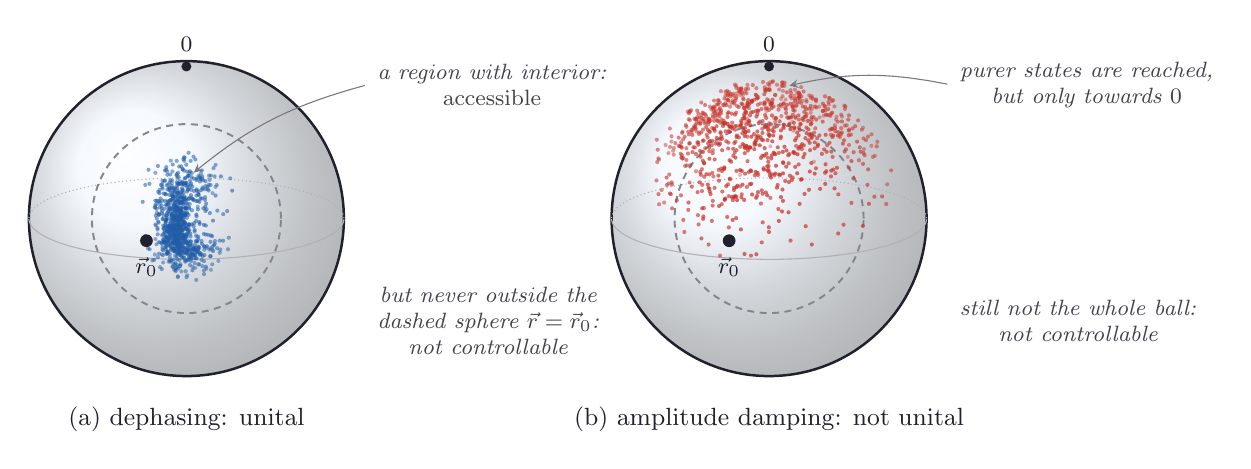
\begin{tikzpicture}[ink/.style={line width=0.9pt, ndInk}, faint/.style={line width=0.4pt, ndInk!35}, dashedink/.style={line width=0.5pt, ndInk!55, dash pattern=on 2.5pt off 2pt}, vec/.style={->, >=stealth, line width=1.2pt}, note/.style={font=\footnotesize\itshape, text=ndInk!85, align=center}, pointer/.style={->, >=stealth, line width=0.4pt, ndInk!60, shorten >=2pt, shorten <=1pt}, dot/.style={circle, fill=ndInk, inner sep=0pt, minimum size=3.4pt}, wash/.style={fill=ndSky, fill opacity=0.55}, every node/.style={text=ndInk}]
\definecolor{ndInk}{rgb}{0.13,0.13,0.18}
\definecolor{ndPaper}{rgb}{0.99,0.96,0.88}
\definecolor{ndSky}{rgb}{0.84,0.91,0.98}
\definecolor{ndRose}{rgb}{0.98,0.86,0.84}
\definecolor{ndBlue}{rgb}{0.13,0.36,0.66}
\definecolor{ndRed}{rgb}{0.78,0.20,0.16}
\definecolor{ndGold}{rgb}{0.88,0.62,0.10}
\definecolor{ndGreen}{rgb}{0.18,0.52,0.30}
\shade[ball color=ndSky!70!white, opacity=0.45] (0.000,0.000) circle (2.000);
\draw[ink] (0.000,0.000) circle (2.000);
\draw[faint] (1.813,-0.219) -- (1.834,-0.206) -- (1.854,-0.194) -- (1.873,-0.181) -- (1.891,-0.169) -- (1.907,-0.156) -- (1.923,-0.143) -- (1.936,-0.130) -- (1.949,-0.116) -- (1.960,-0.103) -- (1.970,-0.090) -- (1.978,-0.077) -- (1.985,-0.063) -- (1.991,-0.050) -- (1.995,-0.036) -- (1.998,-0.023) -- (2.000,-0.009);
\draw[faint] (-2.000,-0.005) -- (-1.999,-0.018) -- (-1.996,-0.032) -- (-1.992,-0.045) -- (-1.987,-0.059) -- (-1.981,-0.072) -- (-1.973,-0.085) -- (-1.963,-0.099) -- (-1.953,-0.112) -- (-1.941,-0.125) -- (-1.927,-0.138) -- (-1.913,-0.151) -- (-1.897,-0.164) -- (-1.879,-0.177) -- (-1.861,-0.190) -- (-1.841,-0.202) -- (-1.820,-0.215) -- (-1.798,-0.227) -- (-1.774,-0.239) -- (-1.749,-0.251) -- (-1.723,-0.263) -- (-1.696,-0.274) -- (-1.668,-0.286) -- (-1.638,-0.297) -- (-1.608,-0.308) -- (-1.576,-0.319) -- (-1.543,-0.329) -- (-1.509,-0.340) -- (-1.475,-0.350) -- (-1.439,-0.360) -- (-1.402,-0.369) -- (-1.364,-0.379) -- (-1.325,-0.388) -- (-1.286,-0.397) -- (-1.245,-0.405) -- (-1.204,-0.413) -- (-1.161,-0.421) -- (-1.118,-0.429) -- (-1.075,-0.437) -- (-1.030,-0.444) -- (-0.985,-0.451) -- (-0.939,-0.457) -- (-0.892,-0.463) -- (-0.845,-0.469) -- (-0.797,-0.475) -- (-0.749,-0.480) -- (-0.700,-0.485) -- (-0.651,-0.489) -- (-0.601,-0.494) -- (-0.551,-0.498) -- (-0.501,-0.501) -- (-0.450,-0.504) -- (-0.399,-0.507) -- (-0.347,-0.510) -- (-0.296,-0.512) -- (-0.244,-0.514) -- (-0.192,-0.515) -- (-0.140,-0.516) -- (-0.087,-0.517) -- (-0.035,-0.518) -- (0.017,-0.518) -- (0.070,-0.517) -- (0.122,-0.517) -- (0.174,-0.516) -- (0.226,-0.514) -- (0.278,-0.513) -- (0.330,-0.511) -- (0.382,-0.508) -- (0.433,-0.505) -- (0.484,-0.502) -- (0.534,-0.499) -- (0.585,-0.495) -- (0.635,-0.491) -- (0.684,-0.486) -- (0.733,-0.482) -- (0.781,-0.476) -- (0.829,-0.471) -- (0.877,-0.465) -- (0.923,-0.459) -- (0.970,-0.453) -- (1.015,-0.446) -- (1.060,-0.439) -- (1.104,-0.432) -- (1.147,-0.424) -- (1.190,-0.416) -- (1.231,-0.408) -- (1.272,-0.399) -- (1.312,-0.391) -- (1.351,-0.382) -- (1.389,-0.372) -- (1.427,-0.363) -- (1.463,-0.353) -- (1.498,-0.343) -- (1.532,-0.333) -- (1.565,-0.322) -- (1.597,-0.312) -- (1.628,-0.301) -- (1.658,-0.289) -- (1.687,-0.278) -- (1.714,-0.267) -- (1.741,-0.255) -- (1.766,-0.243) -- (1.790,-0.231) -- (1.813,-0.219);
\draw[faint, densely dotted] (2.000,0.005) -- (1.999,0.018) -- (1.996,0.032) -- (1.992,0.045) -- (1.987,0.059) -- (1.981,0.072) -- (1.973,0.085) -- (1.963,0.099) -- (1.953,0.112) -- (1.941,0.125) -- (1.927,0.138) -- (1.913,0.151) -- (1.897,0.164) -- (1.879,0.177) -- (1.861,0.190) -- (1.841,0.202) -- (1.820,0.215) -- (1.798,0.227) -- (1.774,0.239) -- (1.749,0.251) -- (1.723,0.263) -- (1.696,0.274) -- (1.668,0.286) -- (1.638,0.297) -- (1.608,0.308) -- (1.576,0.319) -- (1.543,0.329) -- (1.509,0.340) -- (1.475,0.350) -- (1.439,0.360) -- (1.402,0.369) -- (1.364,0.379) -- (1.325,0.388) -- (1.286,0.397) -- (1.245,0.405) -- (1.204,0.413) -- (1.161,0.421) -- (1.118,0.429) -- (1.075,0.437) -- (1.030,0.444) -- (0.985,0.451) -- (0.939,0.457) -- (0.892,0.463) -- (0.845,0.469) -- (0.797,0.475) -- (0.749,0.480) -- (0.700,0.485) -- (0.651,0.489) -- (0.601,0.494) -- (0.551,0.498) -- (0.501,0.501) -- (0.450,0.504) -- (0.399,0.507) -- (0.347,0.510) -- (0.296,0.512) -- (0.244,0.514) -- (0.192,0.515) -- (0.140,0.516) -- (0.087,0.517) -- (0.035,0.518) -- (-0.017,0.518) -- (-0.070,0.517) -- (-0.122,0.517) -- (-0.174,0.516) -- (-0.226,0.514) -- (-0.278,0.513) -- (-0.330,0.511) -- (-0.382,0.508) -- (-0.433,0.505) -- (-0.484,0.502) -- (-0.534,0.499) -- (-0.585,0.495) -- (-0.635,0.491) -- (-0.684,0.486) -- (-0.733,0.482) -- (-0.781,0.476) -- (-0.829,0.471) -- (-0.877,0.465) -- (-0.923,0.459) -- (-0.970,0.453) -- (-1.015,0.446) -- (-1.060,0.439) -- (-1.104,0.432) -- (-1.147,0.424) -- (-1.190,0.416) -- (-1.231,0.408) -- (-1.272,0.399) -- (-1.312,0.391) -- (-1.351,0.382) -- (-1.389,0.372) -- (-1.427,0.363) -- (-1.463,0.353) -- (-1.498,0.343) -- (-1.532,0.333) -- (-1.565,0.322) -- (-1.597,0.312) -- (-1.628,0.301) -- (-1.658,0.289) -- (-1.687,0.278) -- (-1.714,0.267) -- (-1.741,0.255) -- (-1.766,0.243) -- (-1.790,0.231) -- (-1.813,0.219) -- (-1.834,0.206) -- (-1.854,0.194) -- (-1.873,0.181) -- (-1.891,0.169) -- (-1.907,0.156) -- (-1.923,0.143) -- (-1.936,0.130) -- (-1.949,0.116) -- (-1.960,0.103) -- (-1.970,0.090) -- (-1.978,0.077) -- (-1.985,0.063) -- (-1.991,0.050) -- (-1.995,0.036) -- (-1.998,0.023) -- (-2.000,0.009);
\draw[dashedink, line width=0.7pt] (0.000,0.000) circle (1.200);
\fill[ndBlue, opacity=0.45] (0.311,-0.650) circle (0.75pt);
\fill[ndBlue, opacity=0.45] (-0.311,-0.456) circle (0.75pt);
\fill[ndBlue, opacity=0.45] (0.144,0.151) circle (0.75pt);
\fill[ndBlue, opacity=0.45] (0.245,-0.203) circle (0.75pt);
\fill[ndBlue, opacity=0.45] (0.332,-0.395) circle (0.75pt);
\fill[ndBlue, opacity=0.46] (-0.175,-0.304) circle (0.75pt);
\fill[ndBlue, opacity=0.46] (0.038,-0.148) circle (0.75pt);
\fill[ndBlue, opacity=0.46] (0.112,-0.465) circle (0.75pt);
\fill[ndBlue, opacity=0.46] (0.406,-0.537) circle (0.75pt);
\fill[ndBlue, opacity=0.46] (0.370,0.402) circle (0.75pt);
\fill[ndBlue, opacity=0.46] (-0.268,-0.173) circle (0.75pt);
\fill[ndBlue, opacity=0.47] (-0.096,-0.411) circle (0.75pt);
\fill[ndBlue, opacity=0.47] (0.129,-0.422) circle (0.75pt);
\fill[ndBlue, opacity=0.47] (0.195,-0.455) circle (0.75pt);
\fill[ndBlue, opacity=0.47] (-0.030,-0.388) circle (0.75pt);
\fill[ndBlue, opacity=0.47] (0.333,0.323) circle (0.75pt);
\fill[ndBlue, opacity=0.47] (-0.329,-0.305) circle (0.75pt);
\fill[ndBlue, opacity=0.47] (-0.109,-0.743) circle (0.75pt);
\fill[ndBlue, opacity=0.47] (-0.111,-0.370) circle (0.75pt);
\fill[ndBlue, opacity=0.47] (0.108,-0.388) circle (0.75pt);
\fill[ndBlue, opacity=0.48] (-0.157,-0.649) circle (0.75pt);
\fill[ndBlue, opacity=0.48] (-0.385,-0.087) circle (0.75pt);
\fill[ndBlue, opacity=0.48] (0.253,-0.636) circle (0.75pt);
\fill[ndBlue, opacity=0.48] (-0.145,-0.586) circle (0.75pt);
\fill[ndBlue, opacity=0.48] (-0.393,-0.259) circle (0.75pt);
\fill[ndBlue, opacity=0.48] (-0.056,-0.420) circle (0.75pt);
\fill[ndBlue, opacity=0.48] (-0.100,-0.387) circle (0.75pt);
\fill[ndBlue, opacity=0.48] (-0.090,-0.388) circle (0.75pt);
\fill[ndBlue, opacity=0.48] (0.001,-0.532) circle (0.75pt);
\fill[ndBlue, opacity=0.48] (-0.211,-0.350) circle (0.75pt);
\fill[ndBlue, opacity=0.48] (-0.209,-0.451) circle (0.75pt);
\fill[ndBlue, opacity=0.48] (0.206,0.397) circle (0.75pt);
\fill[ndBlue, opacity=0.48] (-0.063,-0.671) circle (0.75pt);
\fill[ndBlue, opacity=0.49] (-0.011,-0.428) circle (0.75pt);
\fill[ndBlue, opacity=0.49] (-0.107,-0.733) circle (0.75pt);
\fill[ndBlue, opacity=0.49] (-0.121,-0.585) circle (0.75pt);
\fill[ndBlue, opacity=0.49] (0.118,-0.368) circle (0.75pt);
\fill[ndBlue, opacity=0.49] (0.165,-0.582) circle (0.75pt);
\fill[ndBlue, opacity=0.49] (0.227,-0.396) circle (0.75pt);
\fill[ndBlue, opacity=0.49] (0.214,0.486) circle (0.75pt);
\fill[ndBlue, opacity=0.49] (-0.253,-0.332) circle (0.75pt);
\fill[ndBlue, opacity=0.49] (-0.295,-0.557) circle (0.75pt);
\fill[ndBlue, opacity=0.49] (-0.077,-0.600) circle (0.75pt);
\fill[ndBlue, opacity=0.49] (0.010,-0.721) circle (0.75pt);
\fill[ndBlue, opacity=0.49] (0.155,-0.363) circle (0.75pt);
\fill[ndBlue, opacity=0.49] (-0.105,-0.270) circle (0.75pt);
\fill[ndBlue, opacity=0.49] (0.149,-0.580) circle (0.75pt);
\fill[ndBlue, opacity=0.49] (-0.395,0.581) circle (0.75pt);
\fill[ndBlue, opacity=0.49] (0.111,-0.626) circle (0.75pt);
\fill[ndBlue, opacity=0.49] (-0.242,-0.414) circle (0.75pt);
\fill[ndBlue, opacity=0.49] (-0.298,-0.465) circle (0.75pt);
\fill[ndBlue, opacity=0.49] (0.016,-0.379) circle (0.75pt);
\fill[ndBlue, opacity=0.49] (-0.262,-0.360) circle (0.75pt);
\fill[ndBlue, opacity=0.49] (-0.028,0.779) circle (0.75pt);
\fill[ndBlue, opacity=0.49] (-0.244,0.600) circle (0.75pt);
\fill[ndBlue, opacity=0.49] (0.001,-0.745) circle (0.75pt);
\fill[ndBlue, opacity=0.49] (-0.401,-0.456) circle (0.75pt);
\fill[ndBlue, opacity=0.50] (-0.089,-0.527) circle (0.75pt);
\fill[ndBlue, opacity=0.50] (0.063,-0.444) circle (0.75pt);
\fill[ndBlue, opacity=0.50] (0.125,-0.779) circle (0.75pt);
\fill[ndBlue, opacity=0.50] (-0.292,-0.259) circle (0.75pt);
\fill[ndBlue, opacity=0.50] (-0.279,-0.177) circle (0.75pt);
\fill[ndBlue, opacity=0.50] (-0.307,-0.299) circle (0.75pt);
\fill[ndBlue, opacity=0.50] (-0.335,-0.617) circle (0.75pt);
\fill[ndBlue, opacity=0.50] (0.352,-0.337) circle (0.75pt);
\fill[ndBlue, opacity=0.50] (0.070,0.579) circle (0.75pt);
\fill[ndBlue, opacity=0.50] (0.023,-0.526) circle (0.75pt);
\fill[ndBlue, opacity=0.50] (-0.020,0.510) circle (0.75pt);
\fill[ndBlue, opacity=0.50] (-0.178,0.599) circle (0.75pt);
\fill[ndBlue, opacity=0.50] (-0.098,-0.369) circle (0.75pt);
\fill[ndBlue, opacity=0.50] (0.328,-0.581) circle (0.75pt);
\fill[ndBlue, opacity=0.50] (-0.180,0.485) circle (0.75pt);
\fill[ndBlue, opacity=0.50] (0.016,-0.397) circle (0.75pt);
\fill[ndBlue, opacity=0.50] (-0.380,-0.326) circle (0.75pt);
\fill[ndBlue, opacity=0.50] (-0.186,0.450) circle (0.75pt);
\fill[ndBlue, opacity=0.50] (-0.057,-0.494) circle (0.75pt);
\fill[ndBlue, opacity=0.50] (-0.304,-0.361) circle (0.75pt);
\fill[ndBlue, opacity=0.50] (0.183,0.576) circle (0.75pt);
\fill[ndBlue, opacity=0.50] (-0.092,-0.346) circle (0.75pt);
\fill[ndBlue, opacity=0.50] (-0.366,-0.139) circle (0.75pt);
\fill[ndBlue, opacity=0.51] (-0.178,-0.606) circle (0.75pt);
\fill[ndBlue, opacity=0.51] (0.192,-0.524) circle (0.75pt);
\fill[ndBlue, opacity=0.51] (-0.194,-0.362) circle (0.75pt);
\fill[ndBlue, opacity=0.51] (0.180,0.516) circle (0.75pt);
\fill[ndBlue, opacity=0.51] (-0.136,-0.667) circle (0.75pt);
\fill[ndBlue, opacity=0.51] (0.103,-0.391) circle (0.75pt);
\fill[ndBlue, opacity=0.51] (-0.304,-0.391) circle (0.75pt);
\fill[ndBlue, opacity=0.51] (0.014,-0.410) circle (0.75pt);
\fill[ndBlue, opacity=0.51] (-0.047,0.629) circle (0.75pt);
\fill[ndBlue, opacity=0.51] (0.053,-0.511) circle (0.75pt);
\fill[ndBlue, opacity=0.51] (0.339,-0.413) circle (0.75pt);
\fill[ndBlue, opacity=0.51] (-0.466,-0.390) circle (0.75pt);
\fill[ndBlue, opacity=0.51] (-0.271,0.480) circle (0.75pt);
\fill[ndBlue, opacity=0.51] (0.090,-0.503) circle (0.75pt);
\fill[ndBlue, opacity=0.51] (-0.114,0.515) circle (0.75pt);
\fill[ndBlue, opacity=0.51] (-0.083,-0.601) circle (0.75pt);
\fill[ndBlue, opacity=0.51] (-0.100,-0.398) circle (0.75pt);
\fill[ndBlue, opacity=0.51] (-0.051,-0.349) circle (0.75pt);
\fill[ndBlue, opacity=0.51] (0.363,-0.284) circle (0.75pt);
\fill[ndBlue, opacity=0.51] (0.051,-0.348) circle (0.75pt);
\fill[ndBlue, opacity=0.51] (-0.161,-0.415) circle (0.75pt);
\fill[ndBlue, opacity=0.51] (-0.138,-0.563) circle (0.75pt);
\fill[ndBlue, opacity=0.51] (0.038,-0.456) circle (0.75pt);
\fill[ndBlue, opacity=0.51] (0.311,0.546) circle (0.75pt);
\fill[ndBlue, opacity=0.51] (-0.198,0.736) circle (0.75pt);
\fill[ndBlue, opacity=0.51] (0.529,-0.389) circle (0.75pt);
\fill[ndBlue, opacity=0.51] (-0.255,0.623) circle (0.75pt);
\fill[ndBlue, opacity=0.51] (0.424,-0.433) circle (0.75pt);
\fill[ndBlue, opacity=0.51] (-0.050,0.469) circle (0.75pt);
\fill[ndBlue, opacity=0.51] (-0.282,-0.273) circle (0.75pt);
\fill[ndBlue, opacity=0.51] (-0.029,-0.442) circle (0.75pt);
\fill[ndBlue, opacity=0.51] (0.056,0.423) circle (0.75pt);
\fill[ndBlue, opacity=0.51] (0.204,-0.604) circle (0.75pt);
\fill[ndBlue, opacity=0.51] (0.078,-0.612) circle (0.75pt);
\fill[ndBlue, opacity=0.51] (-0.093,-0.314) circle (0.75pt);
\fill[ndBlue, opacity=0.51] (0.308,0.427) circle (0.75pt);
\fill[ndBlue, opacity=0.51] (-0.223,-0.330) circle (0.75pt);
\fill[ndBlue, opacity=0.51] (-0.260,-0.388) circle (0.75pt);
\fill[ndBlue, opacity=0.52] (0.200,0.500) circle (0.75pt);
\fill[ndBlue, opacity=0.52] (0.206,-0.477) circle (0.75pt);
\fill[ndBlue, opacity=0.52] (0.039,0.576) circle (0.75pt);
\fill[ndBlue, opacity=0.52] (-0.394,-0.075) circle (0.75pt);
\fill[ndBlue, opacity=0.52] (0.179,0.501) circle (0.75pt);
\fill[ndBlue, opacity=0.52] (0.028,0.544) circle (0.75pt);
\fill[ndBlue, opacity=0.52] (-0.487,-0.378) circle (0.75pt);
\fill[ndBlue, opacity=0.52] (-0.192,-0.308) circle (0.75pt);
\fill[ndBlue, opacity=0.52] (0.154,0.543) circle (0.75pt);
\fill[ndBlue, opacity=0.52] (-0.142,-0.468) circle (0.75pt);
\fill[ndBlue, opacity=0.52] (-0.037,-0.366) circle (0.75pt);
\fill[ndBlue, opacity=0.52] (-0.362,-0.489) circle (0.75pt);
\fill[ndBlue, opacity=0.52] (-0.242,-0.425) circle (0.75pt);
\fill[ndBlue, opacity=0.52] (-0.234,-0.443) circle (0.75pt);
\fill[ndBlue, opacity=0.52] (-0.294,-0.198) circle (0.75pt);
\fill[ndBlue, opacity=0.52] (0.105,-0.564) circle (0.75pt);
\fill[ndBlue, opacity=0.52] (-0.279,-0.293) circle (0.75pt);
\fill[ndBlue, opacity=0.52] (0.222,-0.659) circle (0.75pt);
\fill[ndBlue, opacity=0.52] (-0.295,-0.270) circle (0.75pt);
\fill[ndBlue, opacity=0.52] (0.539,-0.243) circle (0.75pt);
\fill[ndBlue, opacity=0.52] (-0.075,-0.578) circle (0.75pt);
\fill[ndBlue, opacity=0.52] (-0.295,-0.404) circle (0.75pt);
\fill[ndBlue, opacity=0.52] (-0.056,-0.401) circle (0.75pt);
\fill[ndBlue, opacity=0.52] (-0.022,-0.411) circle (0.75pt);
\fill[ndBlue, opacity=0.52] (-0.113,-0.306) circle (0.75pt);
\fill[ndBlue, opacity=0.52] (0.017,-0.407) circle (0.75pt);
\fill[ndBlue, opacity=0.52] (-0.209,-0.530) circle (0.75pt);
\fill[ndBlue, opacity=0.52] (0.044,-0.589) circle (0.75pt);
\fill[ndBlue, opacity=0.52] (-0.009,-0.668) circle (0.75pt);
\fill[ndBlue, opacity=0.52] (-0.288,-0.295) circle (0.75pt);
\fill[ndBlue, opacity=0.52] (0.034,0.393) circle (0.75pt);
\fill[ndBlue, opacity=0.52] (-0.188,-0.530) circle (0.75pt);
\fill[ndBlue, opacity=0.52] (0.360,-0.320) circle (0.75pt);
\fill[ndBlue, opacity=0.52] (0.151,-0.388) circle (0.75pt);
\fill[ndBlue, opacity=0.52] (0.270,0.407) circle (0.75pt);
\fill[ndBlue, opacity=0.52] (0.256,-0.370) circle (0.75pt);
\fill[ndBlue, opacity=0.52] (-0.147,-0.348) circle (0.75pt);
\fill[ndBlue, opacity=0.52] (-0.265,-0.216) circle (0.75pt);
\fill[ndBlue, opacity=0.52] (-0.028,0.734) circle (0.75pt);
\fill[ndBlue, opacity=0.52] (-0.225,-0.547) circle (0.75pt);
\fill[ndBlue, opacity=0.52] (-0.354,0.223) circle (0.75pt);
\fill[ndBlue, opacity=0.52] (-0.123,0.733) circle (0.75pt);
\fill[ndBlue, opacity=0.52] (-0.395,0.228) circle (0.75pt);
\fill[ndBlue, opacity=0.52] (0.231,-0.463) circle (0.75pt);
\fill[ndBlue, opacity=0.53] (-0.108,0.449) circle (0.75pt);
\fill[ndBlue, opacity=0.53] (-0.155,-0.318) circle (0.75pt);
\fill[ndBlue, opacity=0.53] (-0.228,-0.285) circle (0.75pt);
\fill[ndBlue, opacity=0.53] (0.205,0.379) circle (0.75pt);
\fill[ndBlue, opacity=0.53] (0.060,-0.498) circle (0.75pt);
\fill[ndBlue, opacity=0.53] (-0.203,-0.259) circle (0.75pt);
\fill[ndBlue, opacity=0.53] (-0.253,-0.446) circle (0.75pt);
\fill[ndBlue, opacity=0.53] (-0.312,-0.642) circle (0.75pt);
\fill[ndBlue, opacity=0.53] (-0.303,0.380) circle (0.75pt);
\fill[ndBlue, opacity=0.53] (-0.110,-0.376) circle (0.75pt);
\fill[ndBlue, opacity=0.53] (-0.154,-0.380) circle (0.75pt);
\fill[ndBlue, opacity=0.53] (0.149,-0.394) circle (0.75pt);
\fill[ndBlue, opacity=0.53] (0.040,-0.488) circle (0.75pt);
\fill[ndBlue, opacity=0.53] (0.106,-0.465) circle (0.75pt);
\fill[ndBlue, opacity=0.53] (-0.323,0.428) circle (0.75pt);
\fill[ndBlue, opacity=0.53] (0.117,-0.504) circle (0.75pt);
\fill[ndBlue, opacity=0.53] (-0.030,0.609) circle (0.75pt);
\fill[ndBlue, opacity=0.53] (-0.114,-0.443) circle (0.75pt);
\fill[ndBlue, opacity=0.53] (-0.107,-0.408) circle (0.75pt);
\fill[ndBlue, opacity=0.53] (-0.163,-0.519) circle (0.75pt);
\fill[ndBlue, opacity=0.53] (-0.038,-0.496) circle (0.75pt);
\fill[ndBlue, opacity=0.53] (-0.120,-0.275) circle (0.75pt);
\fill[ndBlue, opacity=0.53] (-0.266,-0.364) circle (0.75pt);
\fill[ndBlue, opacity=0.53] (0.227,-0.353) circle (0.75pt);
\fill[ndBlue, opacity=0.53] (0.223,-0.539) circle (0.75pt);
\fill[ndBlue, opacity=0.53] (-0.127,-0.298) circle (0.75pt);
\fill[ndBlue, opacity=0.53] (-0.250,0.424) circle (0.75pt);
\fill[ndBlue, opacity=0.53] (-0.071,-0.363) circle (0.75pt);
\fill[ndBlue, opacity=0.53] (-0.017,-0.531) circle (0.75pt);
\fill[ndBlue, opacity=0.53] (0.295,0.492) circle (0.75pt);
\fill[ndBlue, opacity=0.53] (-0.001,-0.393) circle (0.75pt);
\fill[ndBlue, opacity=0.53] (-0.353,-0.051) circle (0.75pt);
\fill[ndBlue, opacity=0.53] (-0.171,-0.296) circle (0.75pt);
\fill[ndBlue, opacity=0.53] (-0.432,-0.531) circle (0.75pt);
\fill[ndBlue, opacity=0.53] (-0.103,-0.345) circle (0.75pt);
\fill[ndBlue, opacity=0.53] (0.014,-0.518) circle (0.75pt);
\fill[ndBlue, opacity=0.53] (0.224,-0.705) circle (0.75pt);
\fill[ndBlue, opacity=0.53] (-0.044,0.438) circle (0.75pt);
\fill[ndBlue, opacity=0.53] (0.018,-0.404) circle (0.75pt);
\fill[ndBlue, opacity=0.53] (-0.101,-0.634) circle (0.75pt);
\fill[ndBlue, opacity=0.53] (-0.115,-0.275) circle (0.75pt);
\fill[ndBlue, opacity=0.53] (-0.249,-0.288) circle (0.75pt);
\fill[ndBlue, opacity=0.53] (-0.155,-0.279) circle (0.75pt);
\fill[ndBlue, opacity=0.53] (0.386,0.427) circle (0.75pt);
\fill[ndBlue, opacity=0.53] (-0.115,-0.517) circle (0.75pt);
\fill[ndBlue, opacity=0.53] (-0.147,-0.284) circle (0.75pt);
\fill[ndBlue, opacity=0.53] (-0.358,0.339) circle (0.75pt);
\fill[ndBlue, opacity=0.53] (-0.137,-0.418) circle (0.75pt);
\fill[ndBlue, opacity=0.53] (0.306,-0.377) circle (0.75pt);
\fill[ndBlue, opacity=0.53] (-0.303,0.481) circle (0.75pt);
\fill[ndBlue, opacity=0.53] (-0.170,-0.369) circle (0.75pt);
\fill[ndBlue, opacity=0.53] (-0.395,0.142) circle (0.75pt);
\fill[ndBlue, opacity=0.53] (-0.094,-0.303) circle (0.75pt);
\fill[ndBlue, opacity=0.53] (-0.125,0.415) circle (0.75pt);
\fill[ndBlue, opacity=0.53] (0.134,-0.419) circle (0.75pt);
\fill[ndBlue, opacity=0.53] (0.109,-0.333) circle (0.75pt);
\fill[ndBlue, opacity=0.53] (0.556,0.511) circle (0.75pt);
\fill[ndBlue, opacity=0.53] (-0.172,0.283) circle (0.75pt);
\fill[ndBlue, opacity=0.53] (-0.169,-0.616) circle (0.75pt);
\fill[ndBlue, opacity=0.53] (-0.255,-0.239) circle (0.75pt);
\fill[ndBlue, opacity=0.53] (-0.133,-0.306) circle (0.75pt);
\fill[ndBlue, opacity=0.53] (0.430,-0.393) circle (0.75pt);
\fill[ndBlue, opacity=0.53] (0.000,-0.307) circle (0.75pt);
\fill[ndBlue, opacity=0.54] (-0.217,-0.318) circle (0.75pt);
\fill[ndBlue, opacity=0.54] (0.054,0.733) circle (0.75pt);
\fill[ndBlue, opacity=0.54] (-0.254,-0.245) circle (0.75pt);
\fill[ndBlue, opacity=0.54] (-0.045,-0.329) circle (0.75pt);
\fill[ndBlue, opacity=0.54] (-0.203,0.348) circle (0.75pt);
\fill[ndBlue, opacity=0.54] (0.106,-0.418) circle (0.75pt);
\fill[ndBlue, opacity=0.54] (-0.165,-0.318) circle (0.75pt);
\fill[ndBlue, opacity=0.54] (0.028,0.836) circle (0.75pt);
\fill[ndBlue, opacity=0.54] (0.345,0.641) circle (0.75pt);
\fill[ndBlue, opacity=0.54] (-0.120,-0.311) circle (0.75pt);
\fill[ndBlue, opacity=0.54] (-0.137,-0.650) circle (0.75pt);
\fill[ndBlue, opacity=0.54] (-0.224,-0.269) circle (0.75pt);
\fill[ndBlue, opacity=0.54] (-0.291,-0.125) circle (0.75pt);
\fill[ndBlue, opacity=0.54] (-0.131,-0.324) circle (0.75pt);
\fill[ndBlue, opacity=0.54] (-0.064,-0.309) circle (0.75pt);
\fill[ndBlue, opacity=0.54] (-0.018,0.423) circle (0.75pt);
\fill[ndBlue, opacity=0.54] (-0.125,-0.485) circle (0.75pt);
\fill[ndBlue, opacity=0.54] (0.020,-0.346) circle (0.75pt);
\fill[ndBlue, opacity=0.54] (0.077,0.406) circle (0.75pt);
\fill[ndBlue, opacity=0.54] (-0.210,-0.491) circle (0.75pt);
\fill[ndBlue, opacity=0.54] (-0.078,0.320) circle (0.75pt);
\fill[ndBlue, opacity=0.54] (0.070,-0.446) circle (0.75pt);
\fill[ndBlue, opacity=0.54] (0.292,-0.394) circle (0.75pt);
\fill[ndBlue, opacity=0.54] (-0.248,-0.158) circle (0.75pt);
\fill[ndBlue, opacity=0.54] (-0.311,-0.319) circle (0.75pt);
\fill[ndBlue, opacity=0.54] (-0.116,-0.358) circle (0.75pt);
\fill[ndBlue, opacity=0.54] (-0.267,-0.074) circle (0.75pt);
\fill[ndBlue, opacity=0.54] (-0.184,0.289) circle (0.75pt);
\fill[ndBlue, opacity=0.54] (-0.070,-0.368) circle (0.75pt);
\fill[ndBlue, opacity=0.54] (-0.055,-0.321) circle (0.75pt);
\fill[ndBlue, opacity=0.54] (-0.086,-0.458) circle (0.75pt);
\fill[ndBlue, opacity=0.54] (0.090,0.787) circle (0.75pt);
\fill[ndBlue, opacity=0.54] (-0.232,0.431) circle (0.75pt);
\fill[ndBlue, opacity=0.54] (-0.096,-0.438) circle (0.75pt);
\fill[ndBlue, opacity=0.54] (-0.242,0.557) circle (0.75pt);
\fill[ndBlue, opacity=0.54] (-0.261,0.308) circle (0.75pt);
\fill[ndBlue, opacity=0.54] (-0.315,0.128) circle (0.75pt);
\fill[ndBlue, opacity=0.54] (0.302,-0.478) circle (0.75pt);
\fill[ndBlue, opacity=0.54] (-0.522,0.428) circle (0.75pt);
\fill[ndBlue, opacity=0.54] (-0.170,-0.278) circle (0.75pt);
\fill[ndBlue, opacity=0.54] (0.162,-0.429) circle (0.75pt);
\fill[ndBlue, opacity=0.54] (-0.127,-0.250) circle (0.75pt);
\fill[ndBlue, opacity=0.54] (-0.290,0.042) circle (0.75pt);
\fill[ndBlue, opacity=0.54] (-0.228,-0.282) circle (0.75pt);
\fill[ndBlue, opacity=0.54] (0.370,0.682) circle (0.75pt);
\fill[ndBlue, opacity=0.54] (0.237,0.272) circle (0.75pt);
\fill[ndBlue, opacity=0.54] (-0.170,-0.315) circle (0.75pt);
\fill[ndBlue, opacity=0.54] (0.085,-0.378) circle (0.75pt);
\fill[ndBlue, opacity=0.54] (-0.113,0.388) circle (0.75pt);
\fill[ndBlue, opacity=0.54] (-0.367,-0.119) circle (0.75pt);
\fill[ndBlue, opacity=0.54] (-0.338,0.147) circle (0.75pt);
\fill[ndBlue, opacity=0.54] (-0.056,0.386) circle (0.75pt);
\fill[ndBlue, opacity=0.54] (-0.377,0.002) circle (0.75pt);
\fill[ndBlue, opacity=0.54] (-0.278,-0.153) circle (0.75pt);
\fill[ndBlue, opacity=0.54] (-0.115,-0.329) circle (0.75pt);
\fill[ndBlue, opacity=0.54] (0.059,-0.539) circle (0.75pt);
\fill[ndBlue, opacity=0.54] (-0.217,0.364) circle (0.75pt);
\fill[ndBlue, opacity=0.54] (-0.116,-0.243) circle (0.75pt);
\fill[ndBlue, opacity=0.54] (-0.233,0.192) circle (0.75pt);
\fill[ndBlue, opacity=0.54] (-0.119,-0.348) circle (0.75pt);
\fill[ndBlue, opacity=0.54] (-0.205,0.560) circle (0.75pt);
\fill[ndBlue, opacity=0.54] (-0.092,-0.298) circle (0.75pt);
\fill[ndBlue, opacity=0.54] (-0.375,0.072) circle (0.75pt);
\fill[ndBlue, opacity=0.54] (0.071,-0.423) circle (0.75pt);
\fill[ndBlue, opacity=0.54] (-0.099,0.529) circle (0.75pt);
\fill[ndBlue, opacity=0.54] (0.011,-0.314) circle (0.75pt);
\fill[ndBlue, opacity=0.54] (0.289,0.546) circle (0.75pt);
\fill[ndBlue, opacity=0.54] (0.248,-0.610) circle (0.75pt);
\fill[ndBlue, opacity=0.54] (0.390,-0.376) circle (0.75pt);
\fill[ndBlue, opacity=0.54] (0.063,-0.456) circle (0.75pt);
\fill[ndBlue, opacity=0.54] (-0.308,0.438) circle (0.75pt);
\fill[ndBlue, opacity=0.54] (0.468,0.057) circle (0.75pt);
\fill[ndBlue, opacity=0.54] (-0.151,0.348) circle (0.75pt);
\fill[ndBlue, opacity=0.54] (-0.205,-0.244) circle (0.75pt);
\fill[ndBlue, opacity=0.54] (0.101,-0.462) circle (0.75pt);
\fill[ndBlue, opacity=0.54] (0.118,-0.401) circle (0.75pt);
\fill[ndBlue, opacity=0.54] (-0.296,-0.002) circle (0.75pt);
\fill[ndBlue, opacity=0.54] (-0.119,-0.270) circle (0.75pt);
\fill[ndBlue, opacity=0.54] (-0.358,-0.039) circle (0.75pt);
\fill[ndBlue, opacity=0.54] (-0.165,-0.392) circle (0.75pt);
\fill[ndBlue, opacity=0.54] (-0.077,-0.316) circle (0.75pt);
\fill[ndBlue, opacity=0.54] (-0.469,0.442) circle (0.75pt);
\fill[ndBlue, opacity=0.54] (0.308,-0.477) circle (0.75pt);
\fill[ndBlue, opacity=0.54] (-0.288,-0.301) circle (0.75pt);
\fill[ndBlue, opacity=0.54] (0.147,-0.431) circle (0.75pt);
\fill[ndBlue, opacity=0.54] (-0.135,-0.630) circle (0.75pt);
\fill[ndBlue, opacity=0.54] (-0.313,0.165) circle (0.75pt);
\fill[ndBlue, opacity=0.54] (-0.131,-0.214) circle (0.75pt);
\fill[ndBlue, opacity=0.54] (-0.092,0.661) circle (0.75pt);
\fill[ndBlue, opacity=0.54] (-0.158,-0.384) circle (0.75pt);
\fill[ndBlue, opacity=0.54] (0.125,-0.392) circle (0.75pt);
\fill[ndBlue, opacity=0.54] (-0.152,-0.410) circle (0.75pt);
\fill[ndBlue, opacity=0.54] (-0.107,0.439) circle (0.75pt);
\fill[ndBlue, opacity=0.54] (0.222,-0.194) circle (0.75pt);
\fill[ndBlue, opacity=0.54] (0.016,-0.441) circle (0.75pt);
\fill[ndBlue, opacity=0.54] (-0.021,-0.368) circle (0.75pt);
\fill[ndBlue, opacity=0.54] (-0.170,0.230) circle (0.75pt);
\fill[ndBlue, opacity=0.54] (-0.263,-0.096) circle (0.75pt);
\fill[ndBlue, opacity=0.54] (0.177,-0.457) circle (0.75pt);
\fill[ndBlue, opacity=0.54] (-0.246,-0.343) circle (0.75pt);
\fill[ndBlue, opacity=0.54] (0.053,-0.289) circle (0.75pt);
\fill[ndBlue, opacity=0.54] (-0.108,-0.241) circle (0.75pt);
\fill[ndBlue, opacity=0.54] (-0.064,-0.281) circle (0.75pt);
\fill[ndBlue, opacity=0.54] (-0.065,-0.265) circle (0.75pt);
\fill[ndBlue, opacity=0.54] (-0.243,-0.128) circle (0.75pt);
\fill[ndBlue, opacity=0.54] (-0.086,-0.253) circle (0.75pt);
\fill[ndBlue, opacity=0.54] (-0.215,0.457) circle (0.75pt);
\fill[ndBlue, opacity=0.55] (-0.271,0.226) circle (0.75pt);
\fill[ndBlue, opacity=0.55] (-0.151,-0.395) circle (0.75pt);
\fill[ndBlue, opacity=0.55] (-0.117,-0.275) circle (0.75pt);
\fill[ndBlue, opacity=0.55] (-0.306,0.403) circle (0.75pt);
\fill[ndBlue, opacity=0.55] (-0.234,-0.097) circle (0.75pt);
\fill[ndBlue, opacity=0.55] (-0.243,-0.148) circle (0.75pt);
\fill[ndBlue, opacity=0.55] (-0.186,0.243) circle (0.75pt);
\fill[ndBlue, opacity=0.55] (-0.160,-0.255) circle (0.75pt);
\fill[ndBlue, opacity=0.55] (-0.186,0.388) circle (0.75pt);
\fill[ndBlue, opacity=0.55] (0.164,-0.370) circle (0.75pt);
\fill[ndBlue, opacity=0.55] (0.132,-0.285) circle (0.75pt);
\fill[ndBlue, opacity=0.55] (-0.263,-0.229) circle (0.75pt);
\fill[ndBlue, opacity=0.55] (-0.250,-0.447) circle (0.75pt);
\fill[ndBlue, opacity=0.55] (-0.152,-0.408) circle (0.75pt);
\fill[ndBlue, opacity=0.55] (-0.019,-0.376) circle (0.75pt);
\fill[ndBlue, opacity=0.55] (-0.347,-0.445) circle (0.75pt);
\fill[ndBlue, opacity=0.55] (-0.019,-0.304) circle (0.75pt);
\fill[ndBlue, opacity=0.55] (-0.408,-0.523) circle (0.75pt);
\fill[ndBlue, opacity=0.55] (-0.481,0.620) circle (0.75pt);
\fill[ndBlue, opacity=0.55] (-0.142,-0.253) circle (0.75pt);
\fill[ndBlue, opacity=0.55] (-0.126,-0.276) circle (0.75pt);
\fill[ndBlue, opacity=0.55] (-0.015,-0.300) circle (0.75pt);
\fill[ndBlue, opacity=0.55] (-0.342,0.363) circle (0.75pt);
\fill[ndBlue, opacity=0.55] (0.172,-0.457) circle (0.75pt);
\fill[ndBlue, opacity=0.55] (-0.031,-0.492) circle (0.75pt);
\fill[ndBlue, opacity=0.55] (0.333,-0.355) circle (0.75pt);
\fill[ndBlue, opacity=0.55] (-0.361,0.668) circle (0.75pt);
\fill[ndBlue, opacity=0.55] (0.018,-0.305) circle (0.75pt);
\fill[ndBlue, opacity=0.55] (-0.133,-0.224) circle (0.75pt);
\fill[ndBlue, opacity=0.55] (-0.239,-0.128) circle (0.75pt);
\fill[ndBlue, opacity=0.55] (-0.223,-0.092) circle (0.75pt);
\fill[ndBlue, opacity=0.55] (-0.154,-0.223) circle (0.75pt);
\fill[ndBlue, opacity=0.55] (-0.337,0.196) circle (0.75pt);
\fill[ndBlue, opacity=0.55] (-0.056,0.437) circle (0.75pt);
\fill[ndBlue, opacity=0.55] (-0.069,-0.444) circle (0.75pt);
\fill[ndBlue, opacity=0.55] (-0.173,0.687) circle (0.75pt);
\fill[ndBlue, opacity=0.55] (-0.252,-0.015) circle (0.75pt);
\fill[ndBlue, opacity=0.55] (-0.152,-0.212) circle (0.75pt);
\fill[ndBlue, opacity=0.55] (-0.310,0.097) circle (0.75pt);
\fill[ndBlue, opacity=0.55] (-0.208,-0.237) circle (0.75pt);
\fill[ndBlue, opacity=0.55] (-0.262,-0.048) circle (0.75pt);
\fill[ndBlue, opacity=0.55] (-0.096,-0.235) circle (0.75pt);
\fill[ndBlue, opacity=0.55] (-0.280,0.481) circle (0.75pt);
\fill[ndBlue, opacity=0.55] (-0.173,-0.192) circle (0.75pt);
\fill[ndBlue, opacity=0.55] (0.261,-0.351) circle (0.75pt);
\fill[ndBlue, opacity=0.55] (0.393,0.101) circle (0.75pt);
\fill[ndBlue, opacity=0.55] (-0.305,0.226) circle (0.75pt);
\fill[ndBlue, opacity=0.55] (-0.051,-0.245) circle (0.75pt);
\fill[ndBlue, opacity=0.55] (-0.101,-0.273) circle (0.75pt);
\fill[ndBlue, opacity=0.55] (-0.116,0.327) circle (0.75pt);
\fill[ndBlue, opacity=0.55] (0.359,0.536) circle (0.75pt);
\fill[ndBlue, opacity=0.55] (-0.148,0.374) circle (0.75pt);
\fill[ndBlue, opacity=0.55] (-0.252,-0.240) circle (0.75pt);
\fill[ndBlue, opacity=0.55] (0.518,0.096) circle (0.75pt);
\fill[ndBlue, opacity=0.55] (-0.213,-0.140) circle (0.75pt);
\fill[ndBlue, opacity=0.55] (-0.015,0.515) circle (0.75pt);
\fill[ndBlue, opacity=0.55] (-0.167,0.379) circle (0.75pt);
\fill[ndBlue, opacity=0.55] (-0.244,-0.290) circle (0.75pt);
\fill[ndBlue, opacity=0.55] (-0.139,-0.228) circle (0.75pt);
\fill[ndBlue, opacity=0.55] (0.060,-0.476) circle (0.75pt);
\fill[ndBlue, opacity=0.55] (0.197,0.257) circle (0.75pt);
\fill[ndBlue, opacity=0.55] (-0.156,-0.176) circle (0.75pt);
\fill[ndBlue, opacity=0.55] (-0.364,-0.200) circle (0.75pt);
\fill[ndBlue, opacity=0.55] (-0.206,-0.112) circle (0.75pt);
\fill[ndBlue, opacity=0.55] (0.148,-0.357) circle (0.75pt);
\fill[ndBlue, opacity=0.55] (-0.143,-0.198) circle (0.75pt);
\fill[ndBlue, opacity=0.55] (-0.066,0.664) circle (0.75pt);
\fill[ndBlue, opacity=0.55] (-0.037,0.326) circle (0.75pt);
\fill[ndBlue, opacity=0.55] (-0.076,-0.332) circle (0.75pt);
\fill[ndBlue, opacity=0.55] (-0.196,-0.145) circle (0.75pt);
\fill[ndBlue, opacity=0.55] (-0.114,-0.295) circle (0.75pt);
\fill[ndBlue, opacity=0.55] (-0.231,-0.169) circle (0.75pt);
\fill[ndBlue, opacity=0.55] (-0.140,-0.210) circle (0.75pt);
\fill[ndBlue, opacity=0.55] (-0.346,0.061) circle (0.75pt);
\fill[ndBlue, opacity=0.55] (-0.379,0.187) circle (0.75pt);
\fill[ndBlue, opacity=0.55] (-0.069,-0.413) circle (0.75pt);
\fill[ndBlue, opacity=0.55] (-0.139,-0.206) circle (0.75pt);
\fill[ndBlue, opacity=0.55] (-0.032,-0.432) circle (0.75pt);
\fill[ndBlue, opacity=0.55] (-0.044,0.257) circle (0.75pt);
\fill[ndBlue, opacity=0.55] (0.243,0.476) circle (0.75pt);
\fill[ndBlue, opacity=0.55] (-0.288,-0.123) circle (0.75pt);
\fill[ndBlue, opacity=0.55] (0.057,0.366) circle (0.75pt);
\fill[ndBlue, opacity=0.55] (0.028,-0.288) circle (0.75pt);
\fill[ndBlue, opacity=0.55] (-0.022,-0.281) circle (0.75pt);
\fill[ndBlue, opacity=0.55] (0.082,-0.387) circle (0.75pt);
\fill[ndBlue, opacity=0.55] (-0.227,-0.196) circle (0.75pt);
\fill[ndBlue, opacity=0.55] (-0.128,-0.222) circle (0.75pt);
\fill[ndBlue, opacity=0.55] (-0.208,0.233) circle (0.75pt);
\fill[ndBlue, opacity=0.55] (0.051,-0.328) circle (0.75pt);
\fill[ndBlue, opacity=0.55] (-0.079,-0.465) circle (0.75pt);
\fill[ndBlue, opacity=0.55] (-0.141,-0.206) circle (0.75pt);
\fill[ndBlue, opacity=0.55] (-0.521,-0.220) circle (0.75pt);
\fill[ndBlue, opacity=0.55] (-0.266,-0.305) circle (0.75pt);
\fill[ndBlue, opacity=0.55] (-0.074,0.280) circle (0.75pt);
\fill[ndBlue, opacity=0.55] (-0.149,-0.241) circle (0.75pt);
\fill[ndBlue, opacity=0.55] (-0.350,-0.299) circle (0.75pt);
\fill[ndBlue, opacity=0.55] (-0.126,-0.189) circle (0.75pt);
\fill[ndBlue, opacity=0.55] (-0.041,-0.254) circle (0.75pt);
\fill[ndBlue, opacity=0.55] (-0.196,0.190) circle (0.75pt);
\fill[ndBlue, opacity=0.55] (-0.127,-0.226) circle (0.75pt);
\fill[ndBlue, opacity=0.55] (0.424,-0.279) circle (0.75pt);
\fill[ndBlue, opacity=0.55] (0.098,-0.367) circle (0.75pt);
\fill[ndBlue, opacity=0.55] (-0.165,-0.573) circle (0.75pt);
\fill[ndBlue, opacity=0.55] (-0.308,-0.211) circle (0.75pt);
\fill[ndBlue, opacity=0.55] (-0.172,-0.122) circle (0.75pt);
\fill[ndBlue, opacity=0.55] (-0.271,-0.104) circle (0.75pt);
\fill[ndBlue, opacity=0.55] (-0.045,0.367) circle (0.75pt);
\fill[ndBlue, opacity=0.55] (0.327,-0.223) circle (0.75pt);
\fill[ndBlue, opacity=0.55] (-0.131,-0.136) circle (0.75pt);
\fill[ndBlue, opacity=0.55] (-0.060,-0.204) circle (0.75pt);
\fill[ndBlue, opacity=0.55] (-0.057,0.211) circle (0.75pt);
\fill[ndBlue, opacity=0.55] (-0.104,-0.192) circle (0.75pt);
\fill[ndBlue, opacity=0.55] (0.000,-0.290) circle (0.75pt);
\fill[ndBlue, opacity=0.55] (-0.146,-0.143) circle (0.75pt);
\fill[ndBlue, opacity=0.55] (-0.203,-0.116) circle (0.75pt);
\fill[ndBlue, opacity=0.55] (-0.074,0.269) circle (0.75pt);
\fill[ndBlue, opacity=0.55] (-0.147,0.388) circle (0.75pt);
\fill[ndBlue, opacity=0.55] (0.181,-0.441) circle (0.75pt);
\fill[ndBlue, opacity=0.55] (0.023,-0.334) circle (0.75pt);
\fill[ndBlue, opacity=0.55] (-0.098,-0.206) circle (0.75pt);
\fill[ndBlue, opacity=0.55] (-0.128,-0.200) circle (0.75pt);
\fill[ndBlue, opacity=0.55] (-0.248,-0.010) circle (0.75pt);
\fill[ndBlue, opacity=0.55] (0.119,-0.287) circle (0.75pt);
\fill[ndBlue, opacity=0.55] (-0.198,-0.046) circle (0.75pt);
\fill[ndBlue, opacity=0.55] (-0.201,-0.105) circle (0.75pt);
\fill[ndBlue, opacity=0.55] (-0.231,0.129) circle (0.75pt);
\fill[ndBlue, opacity=0.55] (-0.328,0.255) circle (0.75pt);
\fill[ndBlue, opacity=0.55] (-0.249,0.068) circle (0.75pt);
\fill[ndBlue, opacity=0.55] (-0.118,-0.144) circle (0.75pt);
\fill[ndBlue, opacity=0.55] (-0.078,-0.189) circle (0.75pt);
\fill[ndBlue, opacity=0.55] (-0.303,-0.007) circle (0.75pt);
\fill[ndBlue, opacity=0.55] (-0.183,-0.141) circle (0.75pt);
\fill[ndBlue, opacity=0.55] (-0.308,0.070) circle (0.75pt);
\fill[ndBlue, opacity=0.55] (-0.212,-0.203) circle (0.75pt);
\fill[ndBlue, opacity=0.55] (-0.069,0.335) circle (0.75pt);
\fill[ndBlue, opacity=0.55] (-0.123,-0.218) circle (0.75pt);
\fill[ndBlue, opacity=0.55] (-0.117,-0.291) circle (0.75pt);
\fill[ndBlue, opacity=0.55] (-0.378,0.227) circle (0.75pt);
\fill[ndBlue, opacity=0.55] (-0.154,-0.146) circle (0.75pt);
\fill[ndBlue, opacity=0.55] (-0.195,-0.127) circle (0.75pt);
\fill[ndBlue, opacity=0.55] (-0.146,0.191) circle (0.75pt);
\fill[ndBlue, opacity=0.55] (0.466,-0.281) circle (0.75pt);
\fill[ndBlue, opacity=0.55] (-0.166,-0.133) circle (0.75pt);
\fill[ndBlue, opacity=0.55] (-0.389,0.040) circle (0.75pt);
\fill[ndBlue, opacity=0.55] (0.283,0.357) circle (0.75pt);
\fill[ndBlue, opacity=0.55] (-0.085,-0.364) circle (0.75pt);
\fill[ndBlue, opacity=0.55] (-0.115,-0.140) circle (0.75pt);
\fill[ndBlue, opacity=0.55] (0.034,-0.485) circle (0.75pt);
\fill[ndBlue, opacity=0.55] (-0.148,-0.178) circle (0.75pt);
\fill[ndBlue, opacity=0.55] (-0.353,0.047) circle (0.75pt);
\fill[ndBlue, opacity=0.55] (-0.256,0.654) circle (0.75pt);
\fill[ndBlue, opacity=0.55] (-0.105,0.582) circle (0.75pt);
\fill[ndBlue, opacity=0.55] (-0.017,-0.258) circle (0.75pt);
\fill[ndBlue, opacity=0.55] (0.237,0.372) circle (0.75pt);
\fill[ndBlue, opacity=0.55] (-0.086,0.442) circle (0.75pt);
\fill[ndBlue, opacity=0.55] (-0.031,-0.264) circle (0.75pt);
\fill[ndBlue, opacity=0.55] (-0.161,0.150) circle (0.75pt);
\fill[ndBlue, opacity=0.55] (-0.185,0.120) circle (0.75pt);
\fill[ndBlue, opacity=0.55] (-0.154,-0.092) circle (0.75pt);
\fill[ndBlue, opacity=0.55] (-0.105,-0.161) circle (0.75pt);
\fill[ndBlue, opacity=0.55] (-0.090,-0.215) circle (0.75pt);
\fill[ndBlue, opacity=0.55] (-0.135,0.163) circle (0.75pt);
\fill[ndBlue, opacity=0.55] (-0.085,0.260) circle (0.75pt);
\fill[ndBlue, opacity=0.56] (-0.281,0.125) circle (0.75pt);
\fill[ndBlue, opacity=0.56] (-0.170,-0.074) circle (0.75pt);
\fill[ndBlue, opacity=0.56] (0.021,0.428) circle (0.75pt);
\fill[ndBlue, opacity=0.56] (-0.343,0.050) circle (0.75pt);
\fill[ndBlue, opacity=0.56] (-0.042,-0.224) circle (0.75pt);
\fill[ndBlue, opacity=0.56] (0.154,0.338) circle (0.75pt);
\fill[ndBlue, opacity=0.56] (-0.130,-0.130) circle (0.75pt);
\fill[ndBlue, opacity=0.56] (-0.265,-0.032) circle (0.75pt);
\fill[ndBlue, opacity=0.56] (-0.034,0.446) circle (0.75pt);
\fill[ndBlue, opacity=0.56] (-0.067,-0.411) circle (0.75pt);
\fill[ndBlue, opacity=0.56] (-0.056,0.213) circle (0.75pt);
\fill[ndBlue, opacity=0.56] (0.114,0.751) circle (0.75pt);
\fill[ndBlue, opacity=0.56] (-0.132,-0.133) circle (0.75pt);
\fill[ndBlue, opacity=0.56] (-0.215,0.141) circle (0.75pt);
\fill[ndBlue, opacity=0.56] (-0.207,-0.216) circle (0.75pt);
\fill[ndBlue, opacity=0.56] (0.076,-0.656) circle (0.75pt);
\fill[ndBlue, opacity=0.56] (-0.113,-0.104) circle (0.75pt);
\fill[ndBlue, opacity=0.56] (0.013,-0.436) circle (0.75pt);
\fill[ndBlue, opacity=0.56] (-0.159,0.002) circle (0.75pt);
\fill[ndBlue, opacity=0.56] (-0.148,0.277) circle (0.75pt);
\fill[ndBlue, opacity=0.56] (0.057,-0.291) circle (0.75pt);
\fill[ndBlue, opacity=0.56] (-0.228,0.097) circle (0.75pt);
\fill[ndBlue, opacity=0.56] (-0.146,0.136) circle (0.75pt);
\fill[ndBlue, opacity=0.56] (-0.092,-0.368) circle (0.75pt);
\fill[ndBlue, opacity=0.56] (-0.197,-0.206) circle (0.75pt);
\fill[ndBlue, opacity=0.56] (0.202,0.537) circle (0.75pt);
\fill[ndBlue, opacity=0.56] (-0.161,-0.218) circle (0.75pt);
\fill[ndBlue, opacity=0.56] (-0.262,-0.027) circle (0.75pt);
\fill[ndBlue, opacity=0.56] (-0.024,-0.217) circle (0.75pt);
\fill[ndBlue, opacity=0.56] (-0.190,-0.381) circle (0.75pt);
\fill[ndBlue, opacity=0.56] (0.225,-0.354) circle (0.75pt);
\fill[ndBlue, opacity=0.56] (0.095,0.506) circle (0.75pt);
\fill[ndBlue, opacity=0.56] (-0.147,0.290) circle (0.75pt);
\fill[ndBlue, opacity=0.56] (-0.145,-0.133) circle (0.75pt);
\fill[ndBlue, opacity=0.56] (0.256,0.118) circle (0.75pt);
\fill[ndBlue, opacity=0.56] (-0.154,0.169) circle (0.75pt);
\fill[ndBlue, opacity=0.56] (-0.153,0.109) circle (0.75pt);
\fill[ndBlue, opacity=0.56] (-0.212,-0.177) circle (0.75pt);
\fill[ndBlue, opacity=0.56] (-0.378,0.123) circle (0.75pt);
\fill[ndBlue, opacity=0.56] (-0.101,0.219) circle (0.75pt);
\fill[ndBlue, opacity=0.56] (-0.202,-0.546) circle (0.75pt);
\fill[ndBlue, opacity=0.56] (-0.058,0.304) circle (0.75pt);
\fill[ndBlue, opacity=0.56] (-0.171,-0.025) circle (0.75pt);
\fill[ndBlue, opacity=0.56] (0.193,-0.285) circle (0.75pt);
\fill[ndBlue, opacity=0.56] (0.131,0.354) circle (0.75pt);
\fill[ndBlue, opacity=0.56] (-0.190,-0.079) circle (0.75pt);
\fill[ndBlue, opacity=0.56] (0.013,-0.207) circle (0.75pt);
\fill[ndBlue, opacity=0.56] (-0.087,0.133) circle (0.75pt);
\fill[ndBlue, opacity=0.56] (-0.140,-0.069) circle (0.75pt);
\fill[ndBlue, opacity=0.56] (-0.141,-0.019) circle (0.75pt);
\fill[ndBlue, opacity=0.56] (0.299,0.070) circle (0.75pt);
\fill[ndBlue, opacity=0.56] (-0.118,-0.157) circle (0.75pt);
\fill[ndBlue, opacity=0.56] (-0.098,-0.116) circle (0.75pt);
\fill[ndBlue, opacity=0.56] (0.167,0.529) circle (0.75pt);
\fill[ndBlue, opacity=0.56] (-0.159,0.018) circle (0.75pt);
\fill[ndBlue, opacity=0.56] (-0.250,0.014) circle (0.75pt);
\fill[ndBlue, opacity=0.56] (0.003,-0.195) circle (0.75pt);
\fill[ndBlue, opacity=0.56] (-0.131,-0.087) circle (0.75pt);
\fill[ndBlue, opacity=0.56] (-0.180,0.305) circle (0.75pt);
\fill[ndBlue, opacity=0.56] (-0.294,-0.088) circle (0.75pt);
\fill[ndBlue, opacity=0.56] (-0.212,-0.060) circle (0.75pt);
\fill[ndBlue, opacity=0.56] (0.087,-0.457) circle (0.75pt);
\fill[ndBlue, opacity=0.56] (-0.091,-0.120) circle (0.75pt);
\fill[ndBlue, opacity=0.56] (0.128,0.293) circle (0.75pt);
\fill[ndBlue, opacity=0.56] (0.242,0.412) circle (0.75pt);
\fill[ndBlue, opacity=0.56] (0.088,-0.385) circle (0.75pt);
\fill[ndBlue, opacity=0.56] (-0.184,0.052) circle (0.75pt);
\fill[ndBlue, opacity=0.56] (-0.006,0.257) circle (0.75pt);
\fill[ndBlue, opacity=0.56] (-0.122,-0.424) circle (0.75pt);
\fill[ndBlue, opacity=0.56] (-0.395,0.168) circle (0.75pt);
\fill[ndBlue, opacity=0.56] (-0.117,-0.228) circle (0.75pt);
\fill[ndBlue, opacity=0.56] (-0.054,-0.207) circle (0.75pt);
\fill[ndBlue, opacity=0.56] (-0.233,-0.420) circle (0.75pt);
\fill[ndBlue, opacity=0.56] (-0.026,0.245) circle (0.75pt);
\fill[ndBlue, opacity=0.56] (-0.181,0.003) circle (0.75pt);
\fill[ndBlue, opacity=0.56] (-0.011,0.452) circle (0.75pt);
\fill[ndBlue, opacity=0.56] (-0.068,0.212) circle (0.75pt);
\fill[ndBlue, opacity=0.56] (-0.230,-0.093) circle (0.75pt);
\fill[ndBlue, opacity=0.56] (-0.253,0.043) circle (0.75pt);
\fill[ndBlue, opacity=0.56] (-0.269,-0.315) circle (0.75pt);
\fill[ndBlue, opacity=0.56] (-0.196,-0.024) circle (0.75pt);
\fill[ndBlue, opacity=0.56] (-0.079,-0.103) circle (0.75pt);
\fill[ndBlue, opacity=0.56] (-0.166,-0.213) circle (0.75pt);
\fill[ndBlue, opacity=0.56] (0.042,0.185) circle (0.75pt);
\fill[ndBlue, opacity=0.56] (-0.259,0.172) circle (0.75pt);
\fill[ndBlue, opacity=0.56] (-0.167,-0.063) circle (0.75pt);
\fill[ndBlue, opacity=0.56] (-0.149,-0.009) circle (0.75pt);
\fill[ndBlue, opacity=0.56] (-0.115,-0.139) circle (0.75pt);
\fill[ndBlue, opacity=0.56] (-0.145,0.212) circle (0.75pt);
\fill[ndBlue, opacity=0.56] (-0.108,-0.085) circle (0.75pt);
\fill[ndBlue, opacity=0.56] (-0.147,0.035) circle (0.75pt);
\fill[ndBlue, opacity=0.56] (-0.177,0.331) circle (0.75pt);
\fill[ndBlue, opacity=0.56] (0.034,0.264) circle (0.75pt);
\fill[ndBlue, opacity=0.56] (-0.065,0.131) circle (0.75pt);
\fill[ndBlue, opacity=0.56] (-0.067,-0.084) circle (0.75pt);
\fill[ndBlue, opacity=0.56] (-0.057,-0.232) circle (0.75pt);
\fill[ndBlue, opacity=0.56] (0.030,0.247) circle (0.75pt);
\fill[ndBlue, opacity=0.56] (-0.180,0.023) circle (0.75pt);
\fill[ndBlue, opacity=0.56] (-0.047,0.262) circle (0.75pt);
\fill[ndBlue, opacity=0.56] (-0.175,-0.249) circle (0.75pt);
\fill[ndBlue, opacity=0.56] (-0.110,-0.075) circle (0.75pt);
\fill[ndBlue, opacity=0.56] (-0.115,0.102) circle (0.75pt);
\fill[ndBlue, opacity=0.56] (-0.034,0.266) circle (0.75pt);
\fill[ndBlue, opacity=0.56] (-0.184,0.042) circle (0.75pt);
\fill[ndBlue, opacity=0.56] (-0.101,-0.020) circle (0.75pt);
\fill[ndBlue, opacity=0.56] (-0.132,0.007) circle (0.75pt);
\fill[ndBlue, opacity=0.56] (-0.070,0.086) circle (0.75pt);
\fill[ndBlue, opacity=0.56] (-0.077,-0.108) circle (0.75pt);
\fill[ndBlue, opacity=0.56] (-0.121,-0.026) circle (0.75pt);
\fill[ndBlue, opacity=0.56] (-0.042,-0.279) circle (0.75pt);
\fill[ndBlue, opacity=0.56] (0.067,0.526) circle (0.75pt);
\fill[ndBlue, opacity=0.56] (-0.180,-0.180) circle (0.75pt);
\fill[ndBlue, opacity=0.56] (-0.084,-0.089) circle (0.75pt);
\fill[ndBlue, opacity=0.56] (-0.150,-0.109) circle (0.75pt);
\fill[ndBlue, opacity=0.56] (-0.092,0.213) circle (0.75pt);
\fill[ndBlue, opacity=0.56] (-0.082,-0.092) circle (0.75pt);
\fill[ndBlue, opacity=0.56] (0.024,0.368) circle (0.75pt);
\fill[ndBlue, opacity=0.56] (-0.081,-0.110) circle (0.75pt);
\fill[ndBlue, opacity=0.56] (-0.134,0.109) circle (0.75pt);
\fill[ndBlue, opacity=0.56] (-0.001,0.684) circle (0.75pt);
\fill[ndBlue, opacity=0.56] (-0.039,0.755) circle (0.75pt);
\fill[ndBlue, opacity=0.56] (-0.136,-0.305) circle (0.75pt);
\fill[ndBlue, opacity=0.56] (-0.230,0.175) circle (0.75pt);
\fill[ndBlue, opacity=0.56] (-0.084,0.218) circle (0.75pt);
\fill[ndBlue, opacity=0.56] (-0.183,0.057) circle (0.75pt);
\fill[ndBlue, opacity=0.56] (-0.102,-0.071) circle (0.75pt);
\fill[ndBlue, opacity=0.56] (-0.122,0.009) circle (0.75pt);
\fill[ndBlue, opacity=0.56] (-0.148,-0.088) circle (0.75pt);
\fill[ndBlue, opacity=0.56] (-0.116,0.142) circle (0.75pt);
\fill[ndBlue, opacity=0.56] (-0.088,-0.202) circle (0.75pt);
\fill[ndBlue, opacity=0.56] (-0.128,0.137) circle (0.75pt);
\fill[ndBlue, opacity=0.56] (0.237,0.238) circle (0.75pt);
\fill[ndBlue, opacity=0.56] (-0.080,-0.239) circle (0.75pt);
\fill[ndBlue, opacity=0.56] (-0.020,-0.245) circle (0.75pt);
\fill[ndBlue, opacity=0.56] (-0.028,-0.104) circle (0.75pt);
\fill[ndBlue, opacity=0.56] (-0.242,0.370) circle (0.75pt);
\fill[ndBlue, opacity=0.56] (-0.110,0.106) circle (0.75pt);
\fill[ndBlue, opacity=0.56] (-0.051,-0.154) circle (0.75pt);
\fill[ndBlue, opacity=0.56] (-0.078,0.076) circle (0.75pt);
\fill[ndBlue, opacity=0.56] (-0.020,0.132) circle (0.75pt);
\fill[ndBlue, opacity=0.56] (0.023,-0.176) circle (0.75pt);
\fill[ndBlue, opacity=0.56] (-0.080,0.077) circle (0.75pt);
\fill[ndBlue, opacity=0.56] (-0.036,0.147) circle (0.75pt);
\fill[ndBlue, opacity=0.56] (0.016,0.536) circle (0.75pt);
\fill[ndBlue, opacity=0.56] (-0.085,0.011) circle (0.75pt);
\fill[ndBlue, opacity=0.56] (-0.131,0.053) circle (0.75pt);
\fill[ndBlue, opacity=0.56] (-0.065,-0.140) circle (0.75pt);
\fill[ndBlue, opacity=0.56] (0.090,0.243) circle (0.75pt);
\fill[ndBlue, opacity=0.56] (-0.206,-0.092) circle (0.75pt);
\fill[ndBlue, opacity=0.56] (0.273,-0.205) circle (0.75pt);
\fill[ndBlue, opacity=0.56] (-0.083,-0.121) circle (0.75pt);
\fill[ndBlue, opacity=0.56] (-0.030,-0.073) circle (0.75pt);
\fill[ndBlue, opacity=0.56] (-0.179,-0.097) circle (0.75pt);
\fill[ndBlue, opacity=0.56] (-0.111,0.280) circle (0.75pt);
\fill[ndBlue, opacity=0.56] (-0.000,0.232) circle (0.75pt);
\fill[ndBlue, opacity=0.56] (-0.089,-0.072) circle (0.75pt);
\fill[ndBlue, opacity=0.56] (-0.025,0.774) circle (0.75pt);
\fill[ndBlue, opacity=0.56] (-0.252,0.178) circle (0.75pt);
\fill[ndBlue, opacity=0.56] (0.022,-0.160) circle (0.75pt);
\fill[ndBlue, opacity=0.56] (-0.079,0.195) circle (0.75pt);
\fill[ndBlue, opacity=0.56] (0.195,0.612) circle (0.75pt);
\fill[ndBlue, opacity=0.56] (-0.097,-0.061) circle (0.75pt);
\fill[ndBlue, opacity=0.56] (-0.087,-0.016) circle (0.75pt);
\fill[ndBlue, opacity=0.56] (-0.108,-0.017) circle (0.75pt);
\fill[ndBlue, opacity=0.56] (-0.067,-0.152) circle (0.75pt);
\fill[ndBlue, opacity=0.56] (-0.208,0.114) circle (0.75pt);
\fill[ndBlue, opacity=0.56] (-0.166,-0.025) circle (0.75pt);
\fill[ndBlue, opacity=0.56] (-0.050,0.207) circle (0.75pt);
\fill[ndBlue, opacity=0.56] (-0.231,0.086) circle (0.75pt);
\fill[ndBlue, opacity=0.56] (-0.093,-0.033) circle (0.75pt);
\fill[ndBlue, opacity=0.56] (-0.007,0.192) circle (0.75pt);
\fill[ndBlue, opacity=0.56] (0.247,-0.088) circle (0.75pt);
\fill[ndBlue, opacity=0.56] (-0.179,0.086) circle (0.75pt);
\fill[ndBlue, opacity=0.56] (-0.044,0.203) circle (0.75pt);
\fill[ndBlue, opacity=0.56] (-0.062,0.035) circle (0.75pt);
\fill[ndBlue, opacity=0.56] (-0.120,0.086) circle (0.75pt);
\fill[ndBlue, opacity=0.56] (0.242,0.096) circle (0.75pt);
\fill[ndBlue, opacity=0.56] (-0.106,0.351) circle (0.75pt);
\fill[ndBlue, opacity=0.56] (-0.119,0.233) circle (0.75pt);
\fill[ndBlue, opacity=0.56] (0.158,0.300) circle (0.75pt);
\fill[ndBlue, opacity=0.56] (0.104,-0.143) circle (0.75pt);
\fill[ndBlue, opacity=0.56] (-0.113,-0.087) circle (0.75pt);
\fill[ndBlue, opacity=0.56] (-0.064,0.133) circle (0.75pt);
\fill[ndBlue, opacity=0.56] (-0.141,0.095) circle (0.75pt);
\fill[ndBlue, opacity=0.56] (-0.226,-0.167) circle (0.75pt);
\fill[ndBlue, opacity=0.56] (-0.072,0.093) circle (0.75pt);
\fill[ndBlue, opacity=0.56] (-0.056,-0.172) circle (0.75pt);
\fill[ndBlue, opacity=0.56] (-0.102,-0.018) circle (0.75pt);
\fill[ndBlue, opacity=0.56] (-0.069,-0.089) circle (0.75pt);
\fill[ndBlue, opacity=0.56] (-0.073,0.024) circle (0.75pt);
\fill[ndBlue, opacity=0.56] (-0.036,-0.045) circle (0.75pt);
\fill[ndBlue, opacity=0.56] (-0.078,0.093) circle (0.75pt);
\fill[ndBlue, opacity=0.56] (-0.074,0.075) circle (0.75pt);
\fill[ndBlue, opacity=0.56] (0.063,0.263) circle (0.75pt);
\fill[ndBlue, opacity=0.56] (-0.104,-0.031) circle (0.75pt);
\fill[ndBlue, opacity=0.56] (-0.073,-0.005) circle (0.75pt);
\fill[ndBlue, opacity=0.56] (-0.088,-0.017) circle (0.75pt);
\fill[ndBlue, opacity=0.56] (-0.114,0.304) circle (0.75pt);
\fill[ndBlue, opacity=0.56] (-0.125,-0.000) circle (0.75pt);
\fill[ndBlue, opacity=0.56] (-0.038,-0.055) circle (0.75pt);
\fill[ndBlue, opacity=0.56] (-0.180,0.062) circle (0.75pt);
\fill[ndBlue, opacity=0.56] (0.306,-0.295) circle (0.75pt);
\fill[ndBlue, opacity=0.56] (0.096,0.351) circle (0.75pt);
\fill[ndBlue, opacity=0.56] (-0.201,0.007) circle (0.75pt);
\fill[ndBlue, opacity=0.56] (-0.184,-0.151) circle (0.75pt);
\fill[ndBlue, opacity=0.56] (0.105,-0.164) circle (0.75pt);
\fill[ndBlue, opacity=0.56] (-0.074,-0.005) circle (0.75pt);
\fill[ndBlue, opacity=0.56] (-0.013,-0.547) circle (0.75pt);
\fill[ndBlue, opacity=0.56] (-0.202,-0.339) circle (0.75pt);
\fill[ndBlue, opacity=0.56] (-0.341,0.219) circle (0.75pt);
\fill[ndBlue, opacity=0.56] (-0.059,0.016) circle (0.75pt);
\fill[ndBlue, opacity=0.56] (0.270,0.375) circle (0.75pt);
\fill[ndBlue, opacity=0.56] (-0.139,0.049) circle (0.75pt);
\fill[ndBlue, opacity=0.56] (-0.093,0.439) circle (0.75pt);
\fill[ndBlue, opacity=0.56] (-0.144,-0.051) circle (0.75pt);
\fill[ndBlue, opacity=0.56] (-0.017,-0.063) circle (0.75pt);
\fill[ndBlue, opacity=0.56] (-0.088,0.030) circle (0.75pt);
\fill[ndBlue, opacity=0.56] (0.073,0.250) circle (0.75pt);
\fill[ndBlue, opacity=0.56] (0.070,0.106) circle (0.75pt);
\fill[ndBlue, opacity=0.56] (-0.090,-0.136) circle (0.75pt);
\fill[ndBlue, opacity=0.56] (-0.239,0.216) circle (0.75pt);
\fill[ndBlue, opacity=0.56] (-0.111,0.175) circle (0.75pt);
\fill[ndBlue, opacity=0.56] (0.151,-0.257) circle (0.75pt);
\fill[ndBlue, opacity=0.56] (-0.083,-0.095) circle (0.75pt);
\fill[ndBlue, opacity=0.56] (0.093,-0.097) circle (0.75pt);
\fill[ndBlue, opacity=0.56] (-0.140,0.121) circle (0.75pt);
\fill[ndBlue, opacity=0.56] (-0.067,0.061) circle (0.75pt);
\fill[ndBlue, opacity=0.56] (-0.031,0.073) circle (0.75pt);
\fill[ndBlue, opacity=0.56] (0.126,0.222) circle (0.75pt);
\fill[ndBlue, opacity=0.56] (-0.105,0.114) circle (0.75pt);
\fill[ndBlue, opacity=0.56] (-0.109,-0.184) circle (0.75pt);
\fill[ndBlue, opacity=0.56] (-0.126,-0.077) circle (0.75pt);
\fill[ndBlue, opacity=0.56] (-0.142,0.237) circle (0.75pt);
\fill[ndBlue, opacity=0.56] (-0.041,-0.105) circle (0.75pt);
\fill[ndBlue, opacity=0.56] (-0.064,-0.102) circle (0.75pt);
\fill[ndBlue, opacity=0.56] (-0.044,0.084) circle (0.75pt);
\fill[ndBlue, opacity=0.56] (-0.078,0.126) circle (0.75pt);
\fill[ndBlue, opacity=0.56] (0.052,-0.227) circle (0.75pt);
\fill[ndBlue, opacity=0.56] (0.251,0.190) circle (0.75pt);
\fill[ndBlue, opacity=0.56] (0.124,-0.218) circle (0.75pt);
\fill[ndBlue, opacity=0.56] (-0.051,-0.039) circle (0.75pt);
\fill[ndBlue, opacity=0.56] (-0.258,-0.015) circle (0.75pt);
\fill[ndBlue, opacity=0.57] (-0.138,0.032) circle (0.75pt);
\fill[ndBlue, opacity=0.57] (0.004,-0.129) circle (0.75pt);
\fill[ndBlue, opacity=0.57] (0.172,0.472) circle (0.75pt);
\fill[ndBlue, opacity=0.57] (0.145,0.225) circle (0.75pt);
\fill[ndBlue, opacity=0.57] (-0.183,0.141) circle (0.75pt);
\fill[ndBlue, opacity=0.57] (0.036,-0.376) circle (0.75pt);
\fill[ndBlue, opacity=0.57] (0.285,0.430) circle (0.75pt);
\fill[ndBlue, opacity=0.57] (-0.181,-0.160) circle (0.75pt);
\fill[ndBlue, opacity=0.57] (-0.072,0.002) circle (0.75pt);
\fill[ndBlue, opacity=0.57] (-0.016,0.046) circle (0.75pt);
\fill[ndBlue, opacity=0.57] (-0.109,-0.441) circle (0.75pt);
\fill[ndBlue, opacity=0.57] (0.222,-0.079) circle (0.75pt);
\fill[ndBlue, opacity=0.57] (0.008,0.063) circle (0.75pt);
\fill[ndBlue, opacity=0.57] (-0.197,-0.400) circle (0.75pt);
\fill[ndBlue, opacity=0.57] (0.146,0.118) circle (0.75pt);
\fill[ndBlue, opacity=0.57] (-0.103,0.121) circle (0.75pt);
\fill[ndBlue, opacity=0.57] (-0.036,0.013) circle (0.75pt);
\fill[ndBlue, opacity=0.57] (-0.079,0.014) circle (0.75pt);
\fill[ndBlue, opacity=0.57] (-0.006,0.131) circle (0.75pt);
\fill[ndBlue, opacity=0.57] (0.371,0.293) circle (0.75pt);
\fill[ndBlue, opacity=0.57] (0.002,-0.241) circle (0.75pt);
\fill[ndBlue, opacity=0.57] (-0.013,0.044) circle (0.75pt);
\fill[ndBlue, opacity=0.57] (-0.218,0.302) circle (0.75pt);
\fill[ndBlue, opacity=0.57] (-0.017,-0.054) circle (0.75pt);
\fill[ndBlue, opacity=0.57] (-0.007,0.119) circle (0.75pt);
\fill[ndBlue, opacity=0.57] (0.050,-0.191) circle (0.75pt);
\fill[ndBlue, opacity=0.57] (-0.555,0.213) circle (0.75pt);
\fill[ndBlue, opacity=0.57] (-0.156,0.165) circle (0.75pt);
\fill[ndBlue, opacity=0.57] (0.006,0.011) circle (0.75pt);
\fill[ndBlue, opacity=0.57] (-0.107,0.257) circle (0.75pt);
\fill[ndBlue, opacity=0.57] (-0.113,-0.008) circle (0.75pt);
\fill[ndBlue, opacity=0.57] (0.188,0.362) circle (0.75pt);
\fill[ndBlue, opacity=0.57] (-0.092,-0.193) circle (0.75pt);
\fill[ndBlue, opacity=0.57] (-0.144,0.026) circle (0.75pt);
\fill[ndBlue, opacity=0.57] (0.065,-0.336) circle (0.75pt);
\fill[ndBlue, opacity=0.57] (-0.123,0.564) circle (0.75pt);
\fill[ndBlue, opacity=0.57] (0.039,-0.080) circle (0.75pt);
\fill[ndBlue, opacity=0.57] (-0.167,0.022) circle (0.75pt);
\fill[ndBlue, opacity=0.57] (-0.113,0.215) circle (0.75pt);
\fill[ndBlue, opacity=0.57] (-0.044,-0.145) circle (0.75pt);
\fill[ndBlue, opacity=0.57] (-0.066,0.110) circle (0.75pt);
\fill[ndBlue, opacity=0.57] (0.056,-0.399) circle (0.75pt);
\fill[ndBlue, opacity=0.57] (0.001,-0.305) circle (0.75pt);
\fill[ndBlue, opacity=0.57] (-0.013,-0.130) circle (0.75pt);
\fill[ndBlue, opacity=0.57] (-0.065,0.072) circle (0.75pt);
\fill[ndBlue, opacity=0.57] (-0.078,0.101) circle (0.75pt);
\fill[ndBlue, opacity=0.57] (-0.027,0.039) circle (0.75pt);
\fill[ndBlue, opacity=0.57] (-0.006,0.141) circle (0.75pt);
\fill[ndBlue, opacity=0.57] (-0.401,0.141) circle (0.75pt);
\fill[ndBlue, opacity=0.57] (-0.024,0.056) circle (0.75pt);
\fill[ndBlue, opacity=0.57] (-0.007,-0.082) circle (0.75pt);
\fill[ndBlue, opacity=0.57] (0.003,-0.447) circle (0.75pt);
\fill[ndBlue, opacity=0.57] (-0.067,-0.145) circle (0.75pt);
\fill[ndBlue, opacity=0.57] (-0.341,0.324) circle (0.75pt);
\fill[ndBlue, opacity=0.57] (-0.039,-0.070) circle (0.75pt);
\fill[ndBlue, opacity=0.57] (-0.237,-0.248) circle (0.75pt);
\fill[ndBlue, opacity=0.57] (0.131,0.371) circle (0.75pt);
\fill[ndBlue, opacity=0.57] (-0.079,0.041) circle (0.75pt);
\fill[ndBlue, opacity=0.57] (-0.052,-0.023) circle (0.75pt);
\fill[ndBlue, opacity=0.57] (-0.099,-0.068) circle (0.75pt);
\fill[ndBlue, opacity=0.57] (-0.084,0.474) circle (0.75pt);
\fill[ndBlue, opacity=0.57] (0.092,0.235) circle (0.75pt);
\fill[ndBlue, opacity=0.57] (-0.066,0.188) circle (0.75pt);
\fill[ndBlue, opacity=0.57] (-0.062,-0.468) circle (0.75pt);
\fill[ndBlue, opacity=0.57] (-0.268,0.314) circle (0.75pt);
\fill[ndBlue, opacity=0.57] (-0.112,0.144) circle (0.75pt);
\fill[ndBlue, opacity=0.57] (-0.198,0.235) circle (0.75pt);
\fill[ndBlue, opacity=0.57] (-0.106,0.034) circle (0.75pt);
\fill[ndBlue, opacity=0.57] (0.582,0.355) circle (0.75pt);
\fill[ndBlue, opacity=0.57] (-0.117,0.077) circle (0.75pt);
\fill[ndBlue, opacity=0.57] (0.028,-0.075) circle (0.75pt);
\fill[ndBlue, opacity=0.57] (-0.039,-0.012) circle (0.75pt);
\fill[ndBlue, opacity=0.57] (-0.142,0.011) circle (0.75pt);
\fill[ndBlue, opacity=0.57] (0.058,0.299) circle (0.75pt);
\fill[ndBlue, opacity=0.57] (-0.013,0.237) circle (0.75pt);
\fill[ndBlue, opacity=0.57] (0.023,0.544) circle (0.75pt);
\fill[ndBlue, opacity=0.57] (0.029,-0.150) circle (0.75pt);
\fill[ndBlue, opacity=0.57] (-0.149,0.184) circle (0.75pt);
\fill[ndBlue, opacity=0.57] (-0.094,-0.178) circle (0.75pt);
\fill[ndBlue, opacity=0.57] (-0.070,-0.117) circle (0.75pt);
\fill[ndBlue, opacity=0.57] (0.131,0.509) circle (0.75pt);
\fill[ndBlue, opacity=0.57] (-0.028,-0.205) circle (0.75pt);
\fill[ndBlue, opacity=0.57] (0.030,-0.071) circle (0.75pt);
\fill[ndBlue, opacity=0.57] (0.148,-0.228) circle (0.75pt);
\fill[ndBlue, opacity=0.57] (-0.005,0.134) circle (0.75pt);
\fill[ndBlue, opacity=0.57] (-0.165,0.260) circle (0.75pt);
\fill[ndBlue, opacity=0.57] (-0.011,0.059) circle (0.75pt);
\fill[ndBlue, opacity=0.57] (-0.123,0.461) circle (0.75pt);
\fill[ndBlue, opacity=0.57] (-0.048,0.626) circle (0.75pt);
\fill[ndBlue, opacity=0.57] (-0.211,0.384) circle (0.75pt);
\fill[ndBlue, opacity=0.57] (-0.168,-0.124) circle (0.75pt);
\fill[ndBlue, opacity=0.57] (0.046,0.480) circle (0.75pt);
\fill[ndBlue, opacity=0.57] (0.338,-0.026) circle (0.75pt);
\fill[ndBlue, opacity=0.57] (0.129,0.028) circle (0.75pt);
\fill[ndBlue, opacity=0.57] (0.008,0.597) circle (0.75pt);
\fill[ndBlue, opacity=0.57] (0.215,0.129) circle (0.75pt);
\fill[ndBlue, opacity=0.57] (0.013,0.186) circle (0.75pt);
\fill[ndBlue, opacity=0.57] (0.028,0.048) circle (0.75pt);
\fill[ndBlue, opacity=0.57] (0.126,0.052) circle (0.75pt);
\fill[ndBlue, opacity=0.57] (0.124,-0.030) circle (0.75pt);
\fill[ndBlue, opacity=0.57] (-0.116,-0.615) circle (0.75pt);
\fill[ndBlue, opacity=0.58] (-0.028,-0.206) circle (0.75pt);
\fill[ndBlue, opacity=0.58] (0.037,-0.400) circle (0.75pt);
\fill[ndBlue, opacity=0.58] (0.059,0.445) circle (0.75pt);
\fill[ndBlue, opacity=0.58] (-0.059,-0.133) circle (0.75pt);
\fill[ndBlue, opacity=0.58] (0.098,-0.058) circle (0.75pt);
\fill[ndBlue, opacity=0.58] (-0.098,-0.017) circle (0.75pt);
\fill[ndBlue, opacity=0.58] (-0.205,0.129) circle (0.75pt);
\fill[ndBlue, opacity=0.58] (-0.094,0.042) circle (0.75pt);
\fill[ndBlue, opacity=0.58] (0.197,-0.320) circle (0.75pt);
\fill[ndBlue, opacity=0.58] (0.239,0.150) circle (0.75pt);
\fill[ndBlue, opacity=0.58] (0.309,-0.213) circle (0.75pt);
\fill[ndBlue, opacity=0.58] (-0.134,0.136) circle (0.75pt);
\fill[ndBlue, opacity=0.58] (0.033,0.127) circle (0.75pt);
\fill[ndBlue, opacity=0.58] (0.138,-0.292) circle (0.75pt);
\fill[ndBlue, opacity=0.58] (-0.023,-0.040) circle (0.75pt);
\fill[ndBlue, opacity=0.58] (-0.286,0.318) circle (0.75pt);
\fill[ndBlue, opacity=0.58] (0.129,0.490) circle (0.75pt);
\fill[ndBlue, opacity=0.58] (-0.024,0.282) circle (0.75pt);
\fill[ndBlue, opacity=0.58] (-0.203,0.488) circle (0.75pt);
\fill[ndBlue, opacity=0.58] (-0.003,-0.220) circle (0.75pt);
\fill[ndBlue, opacity=0.58] (-0.088,0.191) circle (0.75pt);
\fill[ndBlue, opacity=0.58] (-0.173,0.280) circle (0.75pt);
\fill[ndBlue, opacity=0.58] (-0.092,0.117) circle (0.75pt);
\fill[ndBlue, opacity=0.58] (-0.076,-0.040) circle (0.75pt);
\fill[ndBlue, opacity=0.58] (-0.184,0.414) circle (0.75pt);
\fill[ndBlue, opacity=0.58] (0.151,0.310) circle (0.75pt);
\fill[ndBlue, opacity=0.58] (-0.272,0.612) circle (0.75pt);
\fill[ndBlue, opacity=0.58] (-0.029,-0.228) circle (0.75pt);
\fill[ndBlue, opacity=0.58] (-0.050,0.455) circle (0.75pt);
\fill[ndBlue, opacity=0.58] (0.181,0.255) circle (0.75pt);
\fill[ndBlue, opacity=0.58] (-0.219,0.390) circle (0.75pt);
\fill[ndBlue, opacity=0.58] (-0.093,-0.390) circle (0.75pt);
\fill[ndBlue, opacity=0.58] (0.164,0.214) circle (0.75pt);
\fill[ndBlue, opacity=0.58] (-0.151,0.096) circle (0.75pt);
\fill[ndBlue, opacity=0.58] (0.008,0.343) circle (0.75pt);
\fill[ndBlue, opacity=0.58] (-0.214,0.055) circle (0.75pt);
\fill[ndBlue, opacity=0.58] (-0.007,-0.129) circle (0.75pt);
\fill[ndBlue, opacity=0.59] (-0.017,0.446) circle (0.75pt);
\fill[ndBlue, opacity=0.59] (-0.036,0.250) circle (0.75pt);
\fill[ndBlue, opacity=0.59] (0.032,0.142) circle (0.75pt);
\fill[ndBlue, opacity=0.59] (0.005,0.077) circle (0.75pt);
\fill[ndBlue, opacity=0.59] (-0.251,0.037) circle (0.75pt);
\fill[ndBlue, opacity=0.59] (0.169,-0.067) circle (0.75pt);
\fill[ndBlue, opacity=0.59] (-0.113,0.331) circle (0.75pt);
\fill[ndBlue, opacity=0.59] (0.438,0.536) circle (0.75pt);
\fill[ndBlue, opacity=0.59] (-0.086,-0.122) circle (0.75pt);
\fill[ndBlue, opacity=0.59] (0.017,0.369) circle (0.75pt);
\fill[ndBlue, opacity=0.59] (-0.124,0.549) circle (0.75pt);
\fill[ndBlue, opacity=0.59] (-0.224,0.222) circle (0.75pt);
\fill[ndBlue, opacity=0.59] (-0.036,0.190) circle (0.75pt);
\fill[ndBlue, opacity=0.59] (-0.001,0.455) circle (0.75pt);
\fill[ndBlue, opacity=0.59] (-0.152,0.336) circle (0.75pt);
\fill[ndBlue, opacity=0.59] (0.007,0.408) circle (0.75pt);
\fill[ndBlue, opacity=0.59] (-0.059,0.037) circle (0.75pt);
\fill[ndBlue, opacity=0.59] (-0.050,0.354) circle (0.75pt);
\fill[ndBlue, opacity=0.60] (0.165,-0.044) circle (0.75pt);
\fill[ndBlue, opacity=0.60] (0.065,-0.073) circle (0.75pt);
\fill[ndBlue, opacity=0.60] (-0.003,-0.113) circle (0.75pt);
\fill[ndBlue, opacity=0.60] (0.130,-0.505) circle (0.75pt);
\fill[ndBlue, opacity=0.60] (0.025,-0.108) circle (0.75pt);
\fill[ndBlue, opacity=0.60] (-0.100,0.323) circle (0.75pt);
\fill[ndBlue, opacity=0.60] (0.045,0.601) circle (0.75pt);
\node[dot, fill=ndInk, minimum size=4.6pt, label={[font=\footnotesize]below:$\vec r_0$}] at (-0.507,-0.281) {};
\node[dot, minimum size=3.6pt, label={[font=\footnotesize]above:$\ket0$}] at (0.000,1.932) {};
\node[font=\small] at (0.000,-2.550) {(a) dephasing: unital};
\node[note, anchor=west] (n) at (2.30,1.70) {a region with interior:\\ \emph{accessible}};
\draw[pointer] (n.west) to[bend right=12] (0.040,0.541);
\node[note, anchor=west] (n) at (2.30,-1.30) {but never outside the\\ dashed sphere $\abs{\vec r}=\abs{\vec r_0}$:\\ not controllable};
\shade[ball color=ndSky!70!white, opacity=0.45] (7.400,0.000) circle (2.000);
\draw[ink] (7.400,0.000) circle (2.000);
\draw[faint] (9.213,-0.219) -- (9.234,-0.206) -- (9.254,-0.194) -- (9.273,-0.181) -- (9.291,-0.169) -- (9.307,-0.156) -- (9.323,-0.143) -- (9.336,-0.130) -- (9.349,-0.116) -- (9.360,-0.103) -- (9.370,-0.090) -- (9.378,-0.077) -- (9.385,-0.063) -- (9.391,-0.050) -- (9.395,-0.036) -- (9.398,-0.023) -- (9.400,-0.009);
\draw[faint] (5.400,-0.005) -- (5.401,-0.018) -- (5.404,-0.032) -- (5.408,-0.045) -- (5.413,-0.059) -- (5.419,-0.072) -- (5.427,-0.085) -- (5.437,-0.099) -- (5.447,-0.112) -- (5.459,-0.125) -- (5.473,-0.138) -- (5.487,-0.151) -- (5.503,-0.164) -- (5.521,-0.177) -- (5.539,-0.190) -- (5.559,-0.202) -- (5.580,-0.215) -- (5.602,-0.227) -- (5.626,-0.239) -- (5.651,-0.251) -- (5.677,-0.263) -- (5.704,-0.274) -- (5.732,-0.286) -- (5.762,-0.297) -- (5.792,-0.308) -- (5.824,-0.319) -- (5.857,-0.329) -- (5.891,-0.340) -- (5.925,-0.350) -- (5.961,-0.360) -- (5.998,-0.369) -- (6.036,-0.379) -- (6.075,-0.388) -- (6.114,-0.397) -- (6.155,-0.405) -- (6.196,-0.413) -- (6.239,-0.421) -- (6.282,-0.429) -- (6.325,-0.437) -- (6.370,-0.444) -- (6.415,-0.451) -- (6.461,-0.457) -- (6.508,-0.463) -- (6.555,-0.469) -- (6.603,-0.475) -- (6.651,-0.480) -- (6.700,-0.485) -- (6.749,-0.489) -- (6.799,-0.494) -- (6.849,-0.498) -- (6.899,-0.501) -- (6.950,-0.504) -- (7.001,-0.507) -- (7.053,-0.510) -- (7.104,-0.512) -- (7.156,-0.514) -- (7.208,-0.515) -- (7.260,-0.516) -- (7.313,-0.517) -- (7.365,-0.518) -- (7.417,-0.518) -- (7.470,-0.517) -- (7.522,-0.517) -- (7.574,-0.516) -- (7.626,-0.514) -- (7.678,-0.513) -- (7.730,-0.511) -- (7.782,-0.508) -- (7.833,-0.505) -- (7.884,-0.502) -- (7.934,-0.499) -- (7.985,-0.495) -- (8.035,-0.491) -- (8.084,-0.486) -- (8.133,-0.482) -- (8.181,-0.476) -- (8.229,-0.471) -- (8.277,-0.465) -- (8.323,-0.459) -- (8.370,-0.453) -- (8.415,-0.446) -- (8.460,-0.439) -- (8.504,-0.432) -- (8.547,-0.424) -- (8.590,-0.416) -- (8.631,-0.408) -- (8.672,-0.399) -- (8.712,-0.391) -- (8.751,-0.382) -- (8.789,-0.372) -- (8.827,-0.363) -- (8.863,-0.353) -- (8.898,-0.343) -- (8.932,-0.333) -- (8.965,-0.322) -- (8.997,-0.312) -- (9.028,-0.301) -- (9.058,-0.289) -- (9.087,-0.278) -- (9.114,-0.267) -- (9.141,-0.255) -- (9.166,-0.243) -- (9.190,-0.231) -- (9.213,-0.219);
\draw[faint, densely dotted] (9.400,0.005) -- (9.399,0.018) -- (9.396,0.032) -- (9.392,0.045) -- (9.387,0.059) -- (9.381,0.072) -- (9.373,0.085) -- (9.363,0.099) -- (9.353,0.112) -- (9.341,0.125) -- (9.327,0.138) -- (9.313,0.151) -- (9.297,0.164) -- (9.279,0.177) -- (9.261,0.190) -- (9.241,0.202) -- (9.220,0.215) -- (9.198,0.227) -- (9.174,0.239) -- (9.149,0.251) -- (9.123,0.263) -- (9.096,0.274) -- (9.068,0.286) -- (9.038,0.297) -- (9.008,0.308) -- (8.976,0.319) -- (8.943,0.329) -- (8.909,0.340) -- (8.875,0.350) -- (8.839,0.360) -- (8.802,0.369) -- (8.764,0.379) -- (8.725,0.388) -- (8.686,0.397) -- (8.645,0.405) -- (8.604,0.413) -- (8.561,0.421) -- (8.518,0.429) -- (8.475,0.437) -- (8.430,0.444) -- (8.385,0.451) -- (8.339,0.457) -- (8.292,0.463) -- (8.245,0.469) -- (8.197,0.475) -- (8.149,0.480) -- (8.100,0.485) -- (8.051,0.489) -- (8.001,0.494) -- (7.951,0.498) -- (7.901,0.501) -- (7.850,0.504) -- (7.799,0.507) -- (7.747,0.510) -- (7.696,0.512) -- (7.644,0.514) -- (7.592,0.515) -- (7.540,0.516) -- (7.487,0.517) -- (7.435,0.518) -- (7.383,0.518) -- (7.330,0.517) -- (7.278,0.517) -- (7.226,0.516) -- (7.174,0.514) -- (7.122,0.513) -- (7.070,0.511) -- (7.018,0.508) -- (6.967,0.505) -- (6.916,0.502) -- (6.866,0.499) -- (6.815,0.495) -- (6.765,0.491) -- (6.716,0.486) -- (6.667,0.482) -- (6.619,0.476) -- (6.571,0.471) -- (6.523,0.465) -- (6.477,0.459) -- (6.430,0.453) -- (6.385,0.446) -- (6.340,0.439) -- (6.296,0.432) -- (6.253,0.424) -- (6.210,0.416) -- (6.169,0.408) -- (6.128,0.399) -- (6.088,0.391) -- (6.049,0.382) -- (6.011,0.372) -- (5.973,0.363) -- (5.937,0.353) -- (5.902,0.343) -- (5.868,0.333) -- (5.835,0.322) -- (5.803,0.312) -- (5.772,0.301) -- (5.742,0.289) -- (5.713,0.278) -- (5.686,0.267) -- (5.659,0.255) -- (5.634,0.243) -- (5.610,0.231) -- (5.587,0.219) -- (5.566,0.206) -- (5.546,0.194) -- (5.527,0.181) -- (5.509,0.169) -- (5.493,0.156) -- (5.477,0.143) -- (5.464,0.130) -- (5.451,0.116) -- (5.440,0.103) -- (5.430,0.090) -- (5.422,0.077) -- (5.415,0.063) -- (5.409,0.050) -- (5.405,0.036) -- (5.402,0.023) -- (5.400,0.009);
\draw[dashedink, line width=0.7pt] (7.400,0.000) circle (1.200);
\fill[ndRed, opacity=0.34] (7.416,0.918) circle (0.75pt);
\fill[ndRed, opacity=0.34] (7.031,0.555) circle (0.75pt);
\fill[ndRed, opacity=0.36] (7.228,0.995) circle (0.75pt);
\fill[ndRed, opacity=0.36] (7.708,1.116) circle (0.75pt);
\fill[ndRed, opacity=0.38] (7.093,1.062) circle (0.75pt);
\fill[ndRed, opacity=0.38] (7.969,0.722) circle (0.75pt);
\fill[ndRed, opacity=0.38] (7.693,1.230) circle (0.75pt);
\fill[ndRed, opacity=0.38] (7.457,1.279) circle (0.75pt);
\fill[ndRed, opacity=0.39] (7.365,1.366) circle (0.75pt);
\fill[ndRed, opacity=0.39] (7.108,1.228) circle (0.75pt);
\fill[ndRed, opacity=0.39] (7.937,1.256) circle (0.75pt);
\fill[ndRed, opacity=0.39] (8.400,0.783) circle (0.75pt);
\fill[ndRed, opacity=0.40] (6.873,1.203) circle (0.75pt);
\fill[ndRed, opacity=0.40] (7.942,1.244) circle (0.75pt);
\fill[ndRed, opacity=0.40] (7.732,1.296) circle (0.75pt);
\fill[ndRed, opacity=0.40] (7.120,1.269) circle (0.75pt);
\fill[ndRed, opacity=0.40] (6.794,1.335) circle (0.75pt);
\fill[ndRed, opacity=0.41] (7.148,1.456) circle (0.75pt);
\fill[ndRed, opacity=0.41] (6.774,1.223) circle (0.75pt);
\fill[ndRed, opacity=0.41] (7.885,1.240) circle (0.75pt);
\fill[ndRed, opacity=0.42] (8.037,1.422) circle (0.75pt);
\fill[ndRed, opacity=0.42] (7.587,1.149) circle (0.75pt);
\fill[ndRed, opacity=0.42] (7.403,1.480) circle (0.75pt);
\fill[ndRed, opacity=0.42] (7.790,1.480) circle (0.75pt);
\fill[ndRed, opacity=0.42] (6.623,1.267) circle (0.75pt);
\fill[ndRed, opacity=0.42] (7.827,1.495) circle (0.75pt);
\fill[ndRed, opacity=0.42] (8.165,1.314) circle (0.75pt);
\fill[ndRed, opacity=0.43] (7.610,1.512) circle (0.75pt);
\fill[ndRed, opacity=0.43] (8.257,1.294) circle (0.75pt);
\fill[ndRed, opacity=0.43] (6.683,1.322) circle (0.75pt);
\fill[ndRed, opacity=0.43] (7.719,1.560) circle (0.75pt);
\fill[ndRed, opacity=0.43] (7.553,1.521) circle (0.75pt);
\fill[ndRed, opacity=0.43] (7.476,1.572) circle (0.75pt);
\fill[ndRed, opacity=0.43] (7.111,1.435) circle (0.75pt);
\fill[ndRed, opacity=0.44] (7.768,1.531) circle (0.75pt);
\fill[ndRed, opacity=0.44] (8.093,1.307) circle (0.75pt);
\fill[ndRed, opacity=0.44] (7.874,1.508) circle (0.75pt);
\fill[ndRed, opacity=0.44] (7.558,1.424) circle (0.75pt);
\fill[ndRed, opacity=0.44] (7.411,1.631) circle (0.75pt);
\fill[ndRed, opacity=0.45] (7.929,1.345) circle (0.75pt);
\fill[ndRed, opacity=0.45] (8.042,1.285) circle (0.75pt);
\fill[ndRed, opacity=0.45] (8.250,1.258) circle (0.75pt);
\fill[ndRed, opacity=0.45] (7.737,1.423) circle (0.75pt);
\fill[ndRed, opacity=0.45] (8.326,1.297) circle (0.75pt);
\fill[ndRed, opacity=0.45] (6.470,1.190) circle (0.75pt);
\fill[ndRed, opacity=0.45] (6.882,1.500) circle (0.75pt);
\fill[ndRed, opacity=0.46] (7.069,1.532) circle (0.75pt);
\fill[ndRed, opacity=0.46] (6.786,1.217) circle (0.75pt);
\fill[ndRed, opacity=0.46] (6.987,1.590) circle (0.75pt);
\fill[ndRed, opacity=0.46] (8.594,1.155) circle (0.75pt);
\fill[ndRed, opacity=0.46] (7.577,1.621) circle (0.75pt);
\fill[ndRed, opacity=0.46] (7.396,1.501) circle (0.75pt);
\fill[ndRed, opacity=0.46] (7.758,1.598) circle (0.75pt);
\fill[ndRed, opacity=0.46] (7.808,1.465) circle (0.75pt);
\fill[ndRed, opacity=0.46] (6.828,1.437) circle (0.75pt);
\fill[ndRed, opacity=0.46] (6.439,1.134) circle (0.75pt);
\fill[ndRed, opacity=0.46] (8.699,0.924) circle (0.75pt);
\fill[ndRed, opacity=0.46] (6.182,0.861) circle (0.75pt);
\fill[ndRed, opacity=0.47] (8.605,0.883) circle (0.75pt);
\fill[ndRed, opacity=0.47] (7.995,1.506) circle (0.75pt);
\fill[ndRed, opacity=0.47] (6.918,1.470) circle (0.75pt);
\fill[ndRed, opacity=0.47] (6.700,1.423) circle (0.75pt);
\fill[ndRed, opacity=0.47] (7.070,1.578) circle (0.75pt);
\fill[ndRed, opacity=0.47] (6.845,1.559) circle (0.75pt);
\fill[ndRed, opacity=0.48] (8.743,0.798) circle (0.75pt);
\fill[ndRed, opacity=0.48] (6.160,0.978) circle (0.75pt);
\fill[ndRed, opacity=0.48] (6.122,0.832) circle (0.75pt);
\fill[ndRed, opacity=0.48] (7.033,1.613) circle (0.75pt);
\fill[ndRed, opacity=0.48] (7.997,1.489) circle (0.75pt);
\fill[ndRed, opacity=0.48] (8.900,0.435) circle (0.75pt);
\fill[ndRed, opacity=0.48] (7.528,1.639) circle (0.75pt);
\fill[ndRed, opacity=0.48] (6.086,0.935) circle (0.75pt);
\fill[ndRed, opacity=0.48] (8.159,1.531) circle (0.75pt);
\fill[ndRed, opacity=0.48] (7.358,1.613) circle (0.75pt);
\fill[ndRed, opacity=0.48] (7.449,1.745) circle (0.75pt);
\fill[ndRed, opacity=0.49] (7.946,1.554) circle (0.75pt);
\fill[ndRed, opacity=0.49] (6.757,1.505) circle (0.75pt);
\fill[ndRed, opacity=0.49] (6.594,1.228) circle (0.75pt);
\fill[ndRed, opacity=0.49] (6.937,1.502) circle (0.75pt);
\fill[ndRed, opacity=0.49] (7.570,1.688) circle (0.75pt);
\fill[ndRed, opacity=0.49] (7.728,1.637) circle (0.75pt);
\fill[ndRed, opacity=0.49] (6.394,1.251) circle (0.75pt);
\fill[ndRed, opacity=0.49] (6.668,1.385) circle (0.75pt);
\fill[ndRed, opacity=0.49] (7.404,1.645) circle (0.75pt);
\fill[ndRed, opacity=0.49] (8.158,1.451) circle (0.75pt);
\fill[ndRed, opacity=0.49] (7.384,1.712) circle (0.75pt);
\fill[ndRed, opacity=0.49] (7.943,1.393) circle (0.75pt);
\fill[ndRed, opacity=0.50] (7.595,1.685) circle (0.75pt);
\fill[ndRed, opacity=0.50] (7.047,1.647) circle (0.75pt);
\fill[ndRed, opacity=0.50] (6.002,0.751) circle (0.75pt);
\fill[ndRed, opacity=0.50] (5.994,0.765) circle (0.75pt);
\fill[ndRed, opacity=0.50] (6.191,0.898) circle (0.75pt);
\fill[ndRed, opacity=0.50] (6.515,1.094) circle (0.75pt);
\fill[ndRed, opacity=0.50] (7.560,1.684) circle (0.75pt);
\fill[ndRed, opacity=0.50] (7.567,1.724) circle (0.75pt);
\fill[ndRed, opacity=0.50] (6.602,1.301) circle (0.75pt);
\fill[ndRed, opacity=0.50] (6.301,1.104) circle (0.75pt);
\fill[ndRed, opacity=0.50] (7.997,1.514) circle (0.75pt);
\fill[ndRed, opacity=0.50] (7.377,1.402) circle (0.75pt);
\fill[ndRed, opacity=0.50] (7.413,1.730) circle (0.75pt);
\fill[ndRed, opacity=0.50] (7.688,1.529) circle (0.75pt);
\fill[ndRed, opacity=0.50] (7.034,1.572) circle (0.75pt);
\fill[ndRed, opacity=0.50] (8.719,0.784) circle (0.75pt);
\fill[ndRed, opacity=0.50] (7.571,1.554) circle (0.75pt);
\fill[ndRed, opacity=0.50] (6.647,1.422) circle (0.75pt);
\fill[ndRed, opacity=0.50] (6.981,1.690) circle (0.75pt);
\fill[ndRed, opacity=0.50] (6.539,1.277) circle (0.75pt);
\fill[ndRed, opacity=0.50] (6.718,1.315) circle (0.75pt);
\fill[ndRed, opacity=0.51] (7.018,1.619) circle (0.75pt);
\fill[ndRed, opacity=0.51] (6.748,1.320) circle (0.75pt);
\fill[ndRed, opacity=0.51] (7.134,1.648) circle (0.75pt);
\fill[ndRed, opacity=0.51] (6.789,1.618) circle (0.75pt);
\fill[ndRed, opacity=0.51] (7.046,1.655) circle (0.75pt);
\fill[ndRed, opacity=0.51] (6.311,0.770) circle (0.75pt);
\fill[ndRed, opacity=0.51] (6.189,0.811) circle (0.75pt);
\fill[ndRed, opacity=0.51] (7.500,1.700) circle (0.75pt);
\fill[ndRed, opacity=0.51] (6.394,1.367) circle (0.75pt);
\fill[ndRed, opacity=0.51] (8.230,1.425) circle (0.75pt);
\fill[ndRed, opacity=0.52] (8.385,1.185) circle (0.75pt);
\fill[ndRed, opacity=0.52] (8.702,1.071) circle (0.75pt);
\fill[ndRed, opacity=0.52] (6.368,1.358) circle (0.75pt);
\fill[ndRed, opacity=0.52] (8.950,0.613) circle (0.75pt);
\fill[ndRed, opacity=0.52] (6.140,1.144) circle (0.75pt);
\fill[ndRed, opacity=0.52] (6.967,1.175) circle (0.75pt);
\fill[ndRed, opacity=0.52] (7.264,1.542) circle (0.75pt);
\fill[ndRed, opacity=0.52] (8.316,1.321) circle (0.75pt);
\fill[ndRed, opacity=0.52] (7.048,1.641) circle (0.75pt);
\fill[ndRed, opacity=0.52] (8.204,1.346) circle (0.75pt);
\fill[ndRed, opacity=0.52] (6.067,0.204) circle (0.75pt);
\fill[ndRed, opacity=0.52] (7.126,1.697) circle (0.75pt);
\fill[ndRed, opacity=0.52] (7.556,1.302) circle (0.75pt);
\fill[ndRed, opacity=0.52] (7.802,1.199) circle (0.75pt);
\fill[ndRed, opacity=0.52] (8.775,0.976) circle (0.75pt);
\fill[ndRed, opacity=0.52] (7.790,1.515) circle (0.75pt);
\fill[ndRed, opacity=0.52] (6.410,1.377) circle (0.75pt);
\fill[ndRed, opacity=0.52] (6.965,1.702) circle (0.75pt);
\fill[ndRed, opacity=0.52] (7.808,1.670) circle (0.75pt);
\fill[ndRed, opacity=0.52] (6.142,0.910) circle (0.75pt);
\fill[ndRed, opacity=0.52] (7.349,1.629) circle (0.75pt);
\fill[ndRed, opacity=0.53] (6.991,1.431) circle (0.75pt);
\fill[ndRed, opacity=0.53] (7.932,1.535) circle (0.75pt);
\fill[ndRed, opacity=0.53] (6.678,1.152) circle (0.75pt);
\fill[ndRed, opacity=0.53] (6.880,1.577) circle (0.75pt);
\fill[ndRed, opacity=0.53] (6.905,1.422) circle (0.75pt);
\fill[ndRed, opacity=0.53] (6.983,1.661) circle (0.75pt);
\fill[ndRed, opacity=0.53] (8.362,1.182) circle (0.75pt);
\fill[ndRed, opacity=0.53] (7.444,1.736) circle (0.75pt);
\fill[ndRed, opacity=0.53] (6.383,1.337) circle (0.75pt);
\fill[ndRed, opacity=0.53] (8.363,1.392) circle (0.75pt);
\fill[ndRed, opacity=0.53] (6.684,1.397) circle (0.75pt);
\fill[ndRed, opacity=0.53] (6.472,0.601) circle (0.75pt);
\fill[ndRed, opacity=0.53] (7.440,1.471) circle (0.75pt);
\fill[ndRed, opacity=0.53] (6.942,1.586) circle (0.75pt);
\fill[ndRed, opacity=0.53] (8.370,1.424) circle (0.75pt);
\fill[ndRed, opacity=0.53] (6.795,1.258) circle (0.75pt);
\fill[ndRed, opacity=0.53] (6.479,1.107) circle (0.75pt);
\fill[ndRed, opacity=0.53] (8.235,1.185) circle (0.75pt);
\fill[ndRed, opacity=0.54] (6.161,1.046) circle (0.75pt);
\fill[ndRed, opacity=0.54] (6.785,1.085) circle (0.75pt);
\fill[ndRed, opacity=0.54] (7.095,1.615) circle (0.75pt);
\fill[ndRed, opacity=0.54] (6.557,0.988) circle (0.75pt);
\fill[ndRed, opacity=0.54] (8.170,1.530) circle (0.75pt);
\fill[ndRed, opacity=0.54] (7.404,1.696) circle (0.75pt);
\fill[ndRed, opacity=0.54] (7.088,1.272) circle (0.75pt);
\fill[ndRed, opacity=0.54] (6.539,1.475) circle (0.75pt);
\fill[ndRed, opacity=0.54] (7.774,1.557) circle (0.75pt);
\fill[ndRed, opacity=0.54] (5.974,1.002) circle (0.75pt);
\fill[ndRed, opacity=0.54] (6.472,1.262) circle (0.75pt);
\fill[ndRed, opacity=0.54] (7.257,1.445) circle (0.75pt);
\fill[ndRed, opacity=0.54] (6.036,0.363) circle (0.75pt);
\fill[ndRed, opacity=0.54] (7.145,1.403) circle (0.75pt);
\fill[ndRed, opacity=0.54] (7.239,1.656) circle (0.75pt);
\fill[ndRed, opacity=0.54] (6.721,1.284) circle (0.75pt);
\fill[ndRed, opacity=0.54] (6.351,1.166) circle (0.75pt);
\fill[ndRed, opacity=0.54] (6.588,0.894) circle (0.75pt);
\fill[ndRed, opacity=0.54] (6.752,1.501) circle (0.75pt);
\fill[ndRed, opacity=0.54] (7.911,1.564) circle (0.75pt);
\fill[ndRed, opacity=0.54] (7.114,1.591) circle (0.75pt);
\fill[ndRed, opacity=0.55] (8.154,1.481) circle (0.75pt);
\fill[ndRed, opacity=0.55] (8.413,0.647) circle (0.75pt);
\fill[ndRed, opacity=0.55] (6.570,1.336) circle (0.75pt);
\fill[ndRed, opacity=0.55] (7.348,1.470) circle (0.75pt);
\fill[ndRed, opacity=0.55] (6.708,1.338) circle (0.75pt);
\fill[ndRed, opacity=0.55] (7.725,1.370) circle (0.75pt);
\fill[ndRed, opacity=0.55] (6.627,1.201) circle (0.75pt);
\fill[ndRed, opacity=0.55] (8.599,1.018) circle (0.75pt);
\fill[ndRed, opacity=0.55] (6.379,1.262) circle (0.75pt);
\fill[ndRed, opacity=0.55] (8.415,0.935) circle (0.75pt);
\fill[ndRed, opacity=0.55] (6.978,1.525) circle (0.75pt);
\fill[ndRed, opacity=0.55] (6.879,1.504) circle (0.75pt);
\fill[ndRed, opacity=0.55] (6.749,1.243) circle (0.75pt);
\fill[ndRed, opacity=0.55] (5.980,0.718) circle (0.75pt);
\fill[ndRed, opacity=0.55] (7.859,1.418) circle (0.75pt);
\fill[ndRed, opacity=0.55] (6.749,1.337) circle (0.75pt);
\fill[ndRed, opacity=0.55] (6.309,1.008) circle (0.75pt);
\fill[ndRed, opacity=0.55] (6.510,1.074) circle (0.75pt);
\fill[ndRed, opacity=0.55] (6.252,0.924) circle (0.75pt);
\fill[ndRed, opacity=0.55] (7.114,1.421) circle (0.75pt);
\fill[ndRed, opacity=0.55] (7.185,1.489) circle (0.75pt);
\fill[ndRed, opacity=0.55] (8.103,1.433) circle (0.75pt);
\fill[ndRed, opacity=0.55] (8.578,1.130) circle (0.75pt);
\fill[ndRed, opacity=0.55] (8.002,1.411) circle (0.75pt);
\fill[ndRed, opacity=0.55] (6.276,0.824) circle (0.75pt);
\fill[ndRed, opacity=0.55] (7.876,1.485) circle (0.75pt);
\fill[ndRed, opacity=0.55] (7.183,1.496) circle (0.75pt);
\fill[ndRed, opacity=0.55] (7.672,1.630) circle (0.75pt);
\fill[ndRed, opacity=0.55] (7.478,1.230) circle (0.75pt);
\fill[ndRed, opacity=0.55] (6.687,0.869) circle (0.75pt);
\fill[ndRed, opacity=0.55] (7.776,1.601) circle (0.75pt);
\fill[ndRed, opacity=0.55] (7.323,1.735) circle (0.75pt);
\fill[ndRed, opacity=0.55] (7.376,1.515) circle (0.75pt);
\fill[ndRed, opacity=0.56] (7.127,1.039) circle (0.75pt);
\fill[ndRed, opacity=0.56] (7.568,1.731) circle (0.75pt);
\fill[ndRed, opacity=0.56] (6.872,1.567) circle (0.75pt);
\fill[ndRed, opacity=0.56] (7.106,1.648) circle (0.75pt);
\fill[ndRed, opacity=0.56] (6.209,0.959) circle (0.75pt);
\fill[ndRed, opacity=0.56] (8.111,1.419) circle (0.75pt);
\fill[ndRed, opacity=0.56] (8.531,1.247) circle (0.75pt);
\fill[ndRed, opacity=0.56] (8.657,1.042) circle (0.75pt);
\fill[ndRed, opacity=0.56] (6.541,1.094) circle (0.75pt);
\fill[ndRed, opacity=0.56] (6.441,1.155) circle (0.75pt);
\fill[ndRed, opacity=0.56] (6.543,1.315) circle (0.75pt);
\fill[ndRed, opacity=0.56] (8.316,1.149) circle (0.75pt);
\fill[ndRed, opacity=0.56] (7.811,1.552) circle (0.75pt);
\fill[ndRed, opacity=0.56] (6.986,1.551) circle (0.75pt);
\fill[ndRed, opacity=0.56] (8.197,1.493) circle (0.75pt);
\fill[ndRed, opacity=0.56] (7.354,1.634) circle (0.75pt);
\fill[ndRed, opacity=0.56] (8.179,1.305) circle (0.75pt);
\fill[ndRed, opacity=0.56] (7.251,1.530) circle (0.75pt);
\fill[ndRed, opacity=0.56] (6.394,1.355) circle (0.75pt);
\fill[ndRed, opacity=0.56] (6.003,0.182) circle (0.75pt);
\fill[ndRed, opacity=0.56] (6.832,1.525) circle (0.75pt);
\fill[ndRed, opacity=0.56] (6.452,1.266) circle (0.75pt);
\fill[ndRed, opacity=0.56] (6.451,1.174) circle (0.75pt);
\fill[ndRed, opacity=0.56] (7.899,1.243) circle (0.75pt);
\fill[ndRed, opacity=0.56] (6.487,1.372) circle (0.75pt);
\fill[ndRed, opacity=0.56] (7.026,1.614) circle (0.75pt);
\fill[ndRed, opacity=0.56] (6.844,1.464) circle (0.75pt);
\fill[ndRed, opacity=0.56] (6.373,1.104) circle (0.75pt);
\fill[ndRed, opacity=0.57] (6.558,1.244) circle (0.75pt);
\fill[ndRed, opacity=0.57] (7.027,1.172) circle (0.75pt);
\fill[ndRed, opacity=0.57] (7.987,1.147) circle (0.75pt);
\fill[ndRed, opacity=0.57] (7.712,1.464) circle (0.75pt);
\fill[ndRed, opacity=0.57] (7.839,1.615) circle (0.75pt);
\fill[ndRed, opacity=0.57] (7.597,1.725) circle (0.75pt);
\fill[ndRed, opacity=0.57] (6.754,1.451) circle (0.75pt);
\fill[ndRed, opacity=0.57] (7.730,1.524) circle (0.75pt);
\fill[ndRed, opacity=0.57] (8.213,1.504) circle (0.75pt);
\fill[ndRed, opacity=0.57] (6.768,1.387) circle (0.75pt);
\fill[ndRed, opacity=0.57] (6.777,1.403) circle (0.75pt);
\fill[ndRed, opacity=0.57] (6.867,1.622) circle (0.75pt);
\fill[ndRed, opacity=0.57] (6.521,0.860) circle (0.75pt);
\fill[ndRed, opacity=0.57] (7.288,1.462) circle (0.75pt);
\fill[ndRed, opacity=0.57] (6.847,1.608) circle (0.75pt);
\fill[ndRed, opacity=0.57] (7.424,1.446) circle (0.75pt);
\fill[ndRed, opacity=0.57] (8.356,1.434) circle (0.75pt);
\fill[ndRed, opacity=0.57] (8.542,0.741) circle (0.75pt);
\fill[ndRed, opacity=0.57] (6.509,1.235) circle (0.75pt);
\fill[ndRed, opacity=0.57] (8.888,0.186) circle (0.75pt);
\fill[ndRed, opacity=0.57] (6.910,1.583) circle (0.75pt);
\fill[ndRed, opacity=0.57] (7.352,1.171) circle (0.75pt);
\fill[ndRed, opacity=0.57] (6.891,1.606) circle (0.75pt);
\fill[ndRed, opacity=0.57] (6.296,1.089) circle (0.75pt);
\fill[ndRed, opacity=0.57] (6.702,1.499) circle (0.75pt);
\fill[ndRed, opacity=0.57] (6.656,1.247) circle (0.75pt);
\fill[ndRed, opacity=0.57] (8.110,1.553) circle (0.75pt);
\fill[ndRed, opacity=0.57] (7.344,1.667) circle (0.75pt);
\fill[ndRed, opacity=0.57] (6.541,0.851) circle (0.75pt);
\fill[ndRed, opacity=0.58] (7.193,1.697) circle (0.75pt);
\fill[ndRed, opacity=0.58] (7.313,1.141) circle (0.75pt);
\fill[ndRed, opacity=0.58] (8.440,1.066) circle (0.75pt);
\fill[ndRed, opacity=0.58] (7.679,1.593) circle (0.75pt);
\fill[ndRed, opacity=0.58] (6.502,1.334) circle (0.75pt);
\fill[ndRed, opacity=0.58] (7.762,1.477) circle (0.75pt);
\fill[ndRed, opacity=0.58] (8.414,1.311) circle (0.75pt);
\fill[ndRed, opacity=0.58] (6.477,1.216) circle (0.75pt);
\fill[ndRed, opacity=0.58] (7.374,1.644) circle (0.75pt);
\fill[ndRed, opacity=0.58] (6.469,1.143) circle (0.75pt);
\fill[ndRed, opacity=0.58] (6.350,0.894) circle (0.75pt);
\fill[ndRed, opacity=0.58] (7.614,1.390) circle (0.75pt);
\fill[ndRed, opacity=0.58] (6.487,1.287) circle (0.75pt);
\fill[ndRed, opacity=0.58] (8.082,1.366) circle (0.75pt);
\fill[ndRed, opacity=0.58] (7.015,1.650) circle (0.75pt);
\fill[ndRed, opacity=0.58] (7.399,1.379) circle (0.75pt);
\fill[ndRed, opacity=0.58] (7.400,1.636) circle (0.75pt);
\fill[ndRed, opacity=0.58] (6.519,1.284) circle (0.75pt);
\fill[ndRed, opacity=0.58] (6.391,0.460) circle (0.75pt);
\fill[ndRed, opacity=0.58] (6.643,1.107) circle (0.75pt);
\fill[ndRed, opacity=0.58] (7.430,1.470) circle (0.75pt);
\fill[ndRed, opacity=0.58] (5.970,0.485) circle (0.75pt);
\fill[ndRed, opacity=0.58] (7.956,1.522) circle (0.75pt);
\fill[ndRed, opacity=0.58] (8.631,0.996) circle (0.75pt);
\fill[ndRed, opacity=0.58] (6.357,0.676) circle (0.75pt);
\fill[ndRed, opacity=0.58] (8.273,1.232) circle (0.75pt);
\fill[ndRed, opacity=0.58] (8.767,0.918) circle (0.75pt);
\fill[ndRed, opacity=0.58] (7.520,1.383) circle (0.75pt);
\fill[ndRed, opacity=0.58] (8.406,1.258) circle (0.75pt);
\fill[ndRed, opacity=0.58] (6.945,1.479) circle (0.75pt);
\fill[ndRed, opacity=0.58] (5.986,0.875) circle (0.75pt);
\fill[ndRed, opacity=0.58] (6.471,1.262) circle (0.75pt);
\fill[ndRed, opacity=0.58] (7.579,1.455) circle (0.75pt);
\fill[ndRed, opacity=0.58] (7.523,1.432) circle (0.75pt);
\fill[ndRed, opacity=0.58] (6.342,1.187) circle (0.75pt);
\fill[ndRed, opacity=0.59] (7.084,1.305) circle (0.75pt);
\fill[ndRed, opacity=0.59] (7.791,1.577) circle (0.75pt);
\fill[ndRed, opacity=0.59] (7.055,1.596) circle (0.75pt);
\fill[ndRed, opacity=0.59] (6.923,1.163) circle (0.75pt);
\fill[ndRed, opacity=0.59] (6.519,1.207) circle (0.75pt);
\fill[ndRed, opacity=0.59] (7.248,1.526) circle (0.75pt);
\fill[ndRed, opacity=0.59] (6.703,1.242) circle (0.75pt);
\fill[ndRed, opacity=0.59] (6.334,0.669) circle (0.75pt);
\fill[ndRed, opacity=0.59] (7.929,1.432) circle (0.75pt);
\fill[ndRed, opacity=0.59] (7.627,1.604) circle (0.75pt);
\fill[ndRed, opacity=0.59] (6.956,1.461) circle (0.75pt);
\fill[ndRed, opacity=0.59] (8.613,0.805) circle (0.75pt);
\fill[ndRed, opacity=0.59] (6.350,0.744) circle (0.75pt);
\fill[ndRed, opacity=0.59] (6.585,1.211) circle (0.75pt);
\fill[ndRed, opacity=0.59] (6.589,1.323) circle (0.75pt);
\fill[ndRed, opacity=0.59] (7.109,1.339) circle (0.75pt);
\fill[ndRed, opacity=0.59] (6.869,1.513) circle (0.75pt);
\fill[ndRed, opacity=0.59] (7.781,1.592) circle (0.75pt);
\fill[ndRed, opacity=0.59] (6.773,1.477) circle (0.75pt);
\fill[ndRed, opacity=0.59] (6.387,0.953) circle (0.75pt);
\fill[ndRed, opacity=0.59] (6.639,1.267) circle (0.75pt);
\fill[ndRed, opacity=0.59] (6.252,1.028) circle (0.75pt);
\fill[ndRed, opacity=0.59] (7.256,1.373) circle (0.75pt);
\fill[ndRed, opacity=0.59] (7.085,1.278) circle (0.75pt);
\fill[ndRed, opacity=0.59] (6.562,1.131) circle (0.75pt);
\fill[ndRed, opacity=0.59] (6.132,0.560) circle (0.75pt);
\fill[ndRed, opacity=0.59] (7.586,1.465) circle (0.75pt);
\fill[ndRed, opacity=0.59] (6.644,0.980) circle (0.75pt);
\fill[ndRed, opacity=0.59] (6.102,0.425) circle (0.75pt);
\fill[ndRed, opacity=0.59] (6.125,0.445) circle (0.75pt);
\fill[ndRed, opacity=0.59] (7.387,1.133) circle (0.75pt);
\fill[ndRed, opacity=0.59] (7.606,1.407) circle (0.75pt);
\fill[ndRed, opacity=0.59] (6.693,0.535) circle (0.75pt);
\fill[ndRed, opacity=0.59] (6.140,0.319) circle (0.75pt);
\fill[ndRed, opacity=0.59] (6.461,1.161) circle (0.75pt);
\fill[ndRed, opacity=0.59] (6.329,1.040) circle (0.75pt);
\fill[ndRed, opacity=0.59] (8.173,1.129) circle (0.75pt);
\fill[ndRed, opacity=0.59] (6.972,1.500) circle (0.75pt);
\fill[ndRed, opacity=0.59] (7.034,0.912) circle (0.75pt);
\fill[ndRed, opacity=0.59] (7.127,1.473) circle (0.75pt);
\fill[ndRed, opacity=0.60] (7.830,1.423) circle (0.75pt);
\fill[ndRed, opacity=0.60] (7.778,1.534) circle (0.75pt);
\fill[ndRed, opacity=0.60] (6.284,0.968) circle (0.75pt);
\fill[ndRed, opacity=0.60] (8.552,0.905) circle (0.75pt);
\fill[ndRed, opacity=0.60] (7.392,1.122) circle (0.75pt);
\fill[ndRed, opacity=0.60] (6.416,1.105) circle (0.75pt);
\fill[ndRed, opacity=0.60] (7.743,0.923) circle (0.75pt);
\fill[ndRed, opacity=0.60] (8.151,1.391) circle (0.75pt);
\fill[ndRed, opacity=0.60] (6.587,1.443) circle (0.75pt);
\fill[ndRed, opacity=0.60] (8.461,1.145) circle (0.75pt);
\fill[ndRed, opacity=0.60] (6.792,1.371) circle (0.75pt);
\fill[ndRed, opacity=0.60] (6.414,1.126) circle (0.75pt);
\fill[ndRed, opacity=0.60] (7.079,1.405) circle (0.75pt);
\fill[ndRed, opacity=0.60] (8.115,1.376) circle (0.75pt);
\fill[ndRed, opacity=0.60] (7.778,1.257) circle (0.75pt);
\fill[ndRed, opacity=0.60] (7.702,1.319) circle (0.75pt);
\fill[ndRed, opacity=0.60] (6.530,1.207) circle (0.75pt);
\fill[ndRed, opacity=0.60] (7.109,1.196) circle (0.75pt);
\fill[ndRed, opacity=0.60] (8.413,1.116) circle (0.75pt);
\fill[ndRed, opacity=0.60] (6.907,1.554) circle (0.75pt);
\fill[ndRed, opacity=0.60] (7.418,1.449) circle (0.75pt);
\fill[ndRed, opacity=0.60] (7.233,1.365) circle (0.75pt);
\fill[ndRed, opacity=0.60] (6.982,1.346) circle (0.75pt);
\fill[ndRed, opacity=0.60] (7.304,1.392) circle (0.75pt);
\fill[ndRed, opacity=0.60] (8.417,1.132) circle (0.75pt);
\fill[ndRed, opacity=0.60] (6.974,0.977) circle (0.75pt);
\fill[ndRed, opacity=0.60] (6.556,1.346) circle (0.75pt);
\fill[ndRed, opacity=0.60] (7.478,1.569) circle (0.75pt);
\fill[ndRed, opacity=0.60] (8.186,1.064) circle (0.75pt);
\fill[ndRed, opacity=0.60] (8.120,1.322) circle (0.75pt);
\fill[ndRed, opacity=0.60] (8.198,1.144) circle (0.75pt);
\fill[ndRed, opacity=0.60] (7.787,1.549) circle (0.75pt);
\fill[ndRed, opacity=0.60] (8.494,1.174) circle (0.75pt);
\fill[ndRed, opacity=0.61] (6.392,0.958) circle (0.75pt);
\fill[ndRed, opacity=0.61] (8.139,1.315) circle (0.75pt);
\fill[ndRed, opacity=0.61] (6.738,1.451) circle (0.75pt);
\fill[ndRed, opacity=0.61] (7.045,1.241) circle (0.75pt);
\fill[ndRed, opacity=0.61] (7.965,1.288) circle (0.75pt);
\fill[ndRed, opacity=0.61] (7.871,1.389) circle (0.75pt);
\fill[ndRed, opacity=0.61] (7.177,1.478) circle (0.75pt);
\fill[ndRed, opacity=0.61] (7.126,1.461) circle (0.75pt);
\fill[ndRed, opacity=0.61] (6.743,1.244) circle (0.75pt);
\fill[ndRed, opacity=0.61] (6.168,0.130) circle (0.75pt);
\fill[ndRed, opacity=0.61] (7.458,1.425) circle (0.75pt);
\fill[ndRed, opacity=0.61] (6.620,1.030) circle (0.75pt);
\fill[ndRed, opacity=0.61] (6.946,1.561) circle (0.75pt);
\fill[ndRed, opacity=0.61] (6.818,1.444) circle (0.75pt);
\fill[ndRed, opacity=0.61] (6.292,0.900) circle (0.75pt);
\fill[ndRed, opacity=0.61] (7.485,1.271) circle (0.75pt);
\fill[ndRed, opacity=0.61] (6.400,0.678) circle (0.75pt);
\fill[ndRed, opacity=0.61] (6.166,0.432) circle (0.75pt);
\fill[ndRed, opacity=0.61] (6.873,1.336) circle (0.75pt);
\fill[ndRed, opacity=0.61] (6.292,0.807) circle (0.75pt);
\fill[ndRed, opacity=0.61] (7.417,0.263) circle (0.75pt);
\fill[ndRed, opacity=0.61] (7.972,1.092) circle (0.75pt);
\fill[ndRed, opacity=0.61] (7.546,1.446) circle (0.75pt);
\fill[ndRed, opacity=0.61] (7.081,0.934) circle (0.75pt);
\fill[ndRed, opacity=0.61] (7.075,1.514) circle (0.75pt);
\fill[ndRed, opacity=0.61] (7.215,0.938) circle (0.75pt);
\fill[ndRed, opacity=0.61] (8.649,0.429) circle (0.75pt);
\fill[ndRed, opacity=0.61] (8.593,0.695) circle (0.75pt);
\fill[ndRed, opacity=0.61] (7.339,1.474) circle (0.75pt);
\fill[ndRed, opacity=0.61] (6.833,1.203) circle (0.75pt);
\fill[ndRed, opacity=0.61] (7.032,0.409) circle (0.75pt);
\fill[ndRed, opacity=0.61] (6.382,1.070) circle (0.75pt);
\fill[ndRed, opacity=0.62] (6.709,1.412) circle (0.75pt);
\fill[ndRed, opacity=0.62] (8.083,1.459) circle (0.75pt);
\fill[ndRed, opacity=0.62] (8.599,0.833) circle (0.75pt);
\fill[ndRed, opacity=0.62] (6.679,0.580) circle (0.75pt);
\fill[ndRed, opacity=0.62] (7.241,1.563) circle (0.75pt);
\fill[ndRed, opacity=0.62] (7.939,1.287) circle (0.75pt);
\fill[ndRed, opacity=0.62] (6.163,0.460) circle (0.75pt);
\fill[ndRed, opacity=0.62] (7.938,1.208) circle (0.75pt);
\fill[ndRed, opacity=0.62] (6.490,0.969) circle (0.75pt);
\fill[ndRed, opacity=0.62] (7.145,1.243) circle (0.75pt);
\fill[ndRed, opacity=0.62] (7.731,1.499) circle (0.75pt);
\fill[ndRed, opacity=0.62] (7.050,1.462) circle (0.75pt);
\fill[ndRed, opacity=0.62] (6.932,1.218) circle (0.75pt);
\fill[ndRed, opacity=0.62] (6.860,1.442) circle (0.75pt);
\fill[ndRed, opacity=0.62] (7.925,1.076) circle (0.75pt);
\fill[ndRed, opacity=0.62] (6.228,0.233) circle (0.75pt);
\fill[ndRed, opacity=0.62] (7.118,0.401) circle (0.75pt);
\fill[ndRed, opacity=0.62] (6.695,1.143) circle (0.75pt);
\fill[ndRed, opacity=0.62] (8.085,1.368) circle (0.75pt);
\fill[ndRed, opacity=0.62] (7.127,1.429) circle (0.75pt);
\fill[ndRed, opacity=0.62] (6.687,1.409) circle (0.75pt);
\fill[ndRed, opacity=0.62] (6.457,0.904) circle (0.75pt);
\fill[ndRed, opacity=0.62] (6.439,0.905) circle (0.75pt);
\fill[ndRed, opacity=0.62] (8.191,1.336) circle (0.75pt);
\fill[ndRed, opacity=0.62] (6.370,0.826) circle (0.75pt);
\fill[ndRed, opacity=0.62] (8.412,1.058) circle (0.75pt);
\fill[ndRed, opacity=0.62] (5.995,0.311) circle (0.75pt);
\fill[ndRed, opacity=0.62] (6.608,1.064) circle (0.75pt);
\fill[ndRed, opacity=0.62] (7.230,1.574) circle (0.75pt);
\fill[ndRed, opacity=0.62] (6.641,0.855) circle (0.75pt);
\fill[ndRed, opacity=0.62] (8.474,0.843) circle (0.75pt);
\fill[ndRed, opacity=0.62] (7.135,1.506) circle (0.75pt);
\fill[ndRed, opacity=0.62] (8.836,0.282) circle (0.75pt);
\fill[ndRed, opacity=0.62] (6.646,1.100) circle (0.75pt);
\fill[ndRed, opacity=0.62] (7.339,1.580) circle (0.75pt);
\fill[ndRed, opacity=0.62] (6.722,1.371) circle (0.75pt);
\fill[ndRed, opacity=0.62] (7.105,1.356) circle (0.75pt);
\fill[ndRed, opacity=0.62] (7.876,1.327) circle (0.75pt);
\fill[ndRed, opacity=0.62] (7.847,1.354) circle (0.75pt);
\fill[ndRed, opacity=0.62] (6.832,0.639) circle (0.75pt);
\fill[ndRed, opacity=0.62] (7.257,1.055) circle (0.75pt);
\fill[ndRed, opacity=0.62] (8.325,1.234) circle (0.75pt);
\fill[ndRed, opacity=0.62] (7.178,1.494) circle (0.75pt);
\fill[ndRed, opacity=0.62] (7.213,1.511) circle (0.75pt);
\fill[ndRed, opacity=0.62] (8.241,1.112) circle (0.75pt);
\fill[ndRed, opacity=0.62] (8.137,0.932) circle (0.75pt);
\fill[ndRed, opacity=0.62] (6.777,-0.470) circle (0.75pt);
\fill[ndRed, opacity=0.62] (6.547,0.628) circle (0.75pt);
\fill[ndRed, opacity=0.63] (6.497,0.044) circle (0.75pt);
\fill[ndRed, opacity=0.63] (7.983,1.423) circle (0.75pt);
\fill[ndRed, opacity=0.63] (8.298,1.037) circle (0.75pt);
\fill[ndRed, opacity=0.63] (6.768,1.301) circle (0.75pt);
\fill[ndRed, opacity=0.63] (6.633,1.255) circle (0.75pt);
\fill[ndRed, opacity=0.63] (7.061,1.083) circle (0.75pt);
\fill[ndRed, opacity=0.63] (6.792,0.636) circle (0.75pt);
\fill[ndRed, opacity=0.63] (7.750,1.438) circle (0.75pt);
\fill[ndRed, opacity=0.63] (8.359,0.850) circle (0.75pt);
\fill[ndRed, opacity=0.63] (7.910,1.397) circle (0.75pt);
\fill[ndRed, opacity=0.63] (7.329,0.640) circle (0.75pt);
\fill[ndRed, opacity=0.63] (6.733,1.173) circle (0.75pt);
\fill[ndRed, opacity=0.63] (8.323,1.094) circle (0.75pt);
\fill[ndRed, opacity=0.63] (6.983,1.176) circle (0.75pt);
\fill[ndRed, opacity=0.63] (8.201,1.137) circle (0.75pt);
\fill[ndRed, opacity=0.63] (6.722,0.953) circle (0.75pt);
\fill[ndRed, opacity=0.63] (8.518,0.978) circle (0.75pt);
\fill[ndRed, opacity=0.63] (8.279,1.097) circle (0.75pt);
\fill[ndRed, opacity=0.63] (8.081,1.232) circle (0.75pt);
\fill[ndRed, opacity=0.63] (6.829,0.630) circle (0.75pt);
\fill[ndRed, opacity=0.63] (6.099,0.521) circle (0.75pt);
\fill[ndRed, opacity=0.63] (6.780,1.345) circle (0.75pt);
\fill[ndRed, opacity=0.63] (8.352,0.995) circle (0.75pt);
\fill[ndRed, opacity=0.63] (6.889,0.285) circle (0.75pt);
\fill[ndRed, opacity=0.63] (7.707,1.377) circle (0.75pt);
\fill[ndRed, opacity=0.63] (6.968,0.287) circle (0.75pt);
\fill[ndRed, opacity=0.63] (6.687,1.291) circle (0.75pt);
\fill[ndRed, opacity=0.63] (6.848,1.109) circle (0.75pt);
\fill[ndRed, opacity=0.63] (6.822,1.243) circle (0.75pt);
\fill[ndRed, opacity=0.63] (7.094,1.046) circle (0.75pt);
\fill[ndRed, opacity=0.63] (7.670,1.553) circle (0.75pt);
\fill[ndRed, opacity=0.63] (6.710,1.115) circle (0.75pt);
\fill[ndRed, opacity=0.63] (7.141,1.451) circle (0.75pt);
\fill[ndRed, opacity=0.63] (7.240,0.997) circle (0.75pt);
\fill[ndRed, opacity=0.63] (6.548,0.350) circle (0.75pt);
\fill[ndRed, opacity=0.63] (6.699,1.360) circle (0.75pt);
\fill[ndRed, opacity=0.63] (8.562,0.851) circle (0.75pt);
\fill[ndRed, opacity=0.63] (6.886,1.350) circle (0.75pt);
\fill[ndRed, opacity=0.63] (6.282,0.916) circle (0.75pt);
\fill[ndRed, opacity=0.63] (7.999,1.257) circle (0.75pt);
\fill[ndRed, opacity=0.63] (7.317,1.238) circle (0.75pt);
\fill[ndRed, opacity=0.63] (6.763,0.936) circle (0.75pt);
\fill[ndRed, opacity=0.63] (7.468,0.553) circle (0.75pt);
\fill[ndRed, opacity=0.63] (8.737,0.278) circle (0.75pt);
\fill[ndRed, opacity=0.63] (7.117,0.922) circle (0.75pt);
\fill[ndRed, opacity=0.63] (6.643,0.379) circle (0.75pt);
\fill[ndRed, opacity=0.63] (7.014,1.418) circle (0.75pt);
\fill[ndRed, opacity=0.64] (6.152,0.311) circle (0.75pt);
\fill[ndRed, opacity=0.64] (7.406,1.062) circle (0.75pt);
\fill[ndRed, opacity=0.64] (6.814,1.211) circle (0.75pt);
\fill[ndRed, opacity=0.64] (6.642,1.234) circle (0.75pt);
\fill[ndRed, opacity=0.64] (7.657,1.205) circle (0.75pt);
\fill[ndRed, opacity=0.64] (6.925,1.333) circle (0.75pt);
\fill[ndRed, opacity=0.64] (6.778,1.006) circle (0.75pt);
\fill[ndRed, opacity=0.64] (6.901,0.508) circle (0.75pt);
\fill[ndRed, opacity=0.64] (7.265,1.369) circle (0.75pt);
\fill[ndRed, opacity=0.64] (6.945,0.797) circle (0.75pt);
\fill[ndRed, opacity=0.64] (8.011,1.021) circle (0.75pt);
\fill[ndRed, opacity=0.64] (7.487,1.278) circle (0.75pt);
\fill[ndRed, opacity=0.64] (6.569,1.264) circle (0.75pt);
\fill[ndRed, opacity=0.64] (7.404,1.209) circle (0.75pt);
\fill[ndRed, opacity=0.64] (7.700,1.424) circle (0.75pt);
\fill[ndRed, opacity=0.64] (6.684,0.831) circle (0.75pt);
\fill[ndRed, opacity=0.64] (7.868,1.295) circle (0.75pt);
\fill[ndRed, opacity=0.64] (7.772,1.310) circle (0.75pt);
\fill[ndRed, opacity=0.64] (6.601,1.163) circle (0.75pt);
\fill[ndRed, opacity=0.64] (6.872,1.202) circle (0.75pt);
\fill[ndRed, opacity=0.64] (6.967,1.129) circle (0.75pt);
\fill[ndRed, opacity=0.64] (7.076,1.116) circle (0.75pt);
\fill[ndRed, opacity=0.64] (8.659,0.625) circle (0.75pt);
\fill[ndRed, opacity=0.64] (7.285,1.232) circle (0.75pt);
\fill[ndRed, opacity=0.64] (6.281,0.296) circle (0.75pt);
\fill[ndRed, opacity=0.64] (7.617,1.341) circle (0.75pt);
\fill[ndRed, opacity=0.64] (6.311,-0.017) circle (0.75pt);
\fill[ndRed, opacity=0.64] (6.501,0.967) circle (0.75pt);
\fill[ndRed, opacity=0.64] (6.641,0.562) circle (0.75pt);
\fill[ndRed, opacity=0.64] (7.171,1.347) circle (0.75pt);
\fill[ndRed, opacity=0.64] (6.856,0.982) circle (0.75pt);
\fill[ndRed, opacity=0.64] (6.374,0.111) circle (0.75pt);
\fill[ndRed, opacity=0.64] (6.299,0.762) circle (0.75pt);
\fill[ndRed, opacity=0.64] (6.426,1.063) circle (0.75pt);
\fill[ndRed, opacity=0.64] (7.130,0.893) circle (0.75pt);
\fill[ndRed, opacity=0.64] (8.207,0.784) circle (0.75pt);
\fill[ndRed, opacity=0.64] (6.572,0.134) circle (0.75pt);
\fill[ndRed, opacity=0.64] (8.203,1.036) circle (0.75pt);
\fill[ndRed, opacity=0.64] (7.834,1.252) circle (0.75pt);
\fill[ndRed, opacity=0.64] (8.238,1.150) circle (0.75pt);
\fill[ndRed, opacity=0.64] (7.053,0.309) circle (0.75pt);
\fill[ndRed, opacity=0.64] (7.937,1.022) circle (0.75pt);
\fill[ndRed, opacity=0.64] (7.779,1.159) circle (0.75pt);
\fill[ndRed, opacity=0.64] (7.085,1.328) circle (0.75pt);
\fill[ndRed, opacity=0.64] (7.672,1.458) circle (0.75pt);
\fill[ndRed, opacity=0.64] (7.438,1.124) circle (0.75pt);
\fill[ndRed, opacity=0.64] (7.391,1.074) circle (0.75pt);
\fill[ndRed, opacity=0.64] (7.251,1.326) circle (0.75pt);
\fill[ndRed, opacity=0.64] (6.802,1.014) circle (0.75pt);
\fill[ndRed, opacity=0.64] (7.065,1.269) circle (0.75pt);
\fill[ndRed, opacity=0.64] (6.761,0.619) circle (0.75pt);
\fill[ndRed, opacity=0.64] (6.324,-0.170) circle (0.75pt);
\fill[ndRed, opacity=0.64] (7.445,1.511) circle (0.75pt);
\fill[ndRed, opacity=0.65] (6.879,0.436) circle (0.75pt);
\fill[ndRed, opacity=0.65] (6.708,0.390) circle (0.75pt);
\fill[ndRed, opacity=0.65] (6.947,0.271) circle (0.75pt);
\fill[ndRed, opacity=0.65] (7.061,1.450) circle (0.75pt);
\fill[ndRed, opacity=0.65] (6.568,0.992) circle (0.75pt);
\fill[ndRed, opacity=0.65] (7.384,0.773) circle (0.75pt);
\fill[ndRed, opacity=0.65] (6.505,-0.074) circle (0.75pt);
\fill[ndRed, opacity=0.65] (6.815,1.175) circle (0.75pt);
\fill[ndRed, opacity=0.65] (6.472,0.821) circle (0.75pt);
\fill[ndRed, opacity=0.65] (7.715,1.216) circle (0.75pt);
\fill[ndRed, opacity=0.65] (7.423,1.198) circle (0.75pt);
\fill[ndRed, opacity=0.65] (8.311,1.072) circle (0.75pt);
\fill[ndRed, opacity=0.65] (7.432,1.461) circle (0.75pt);
\fill[ndRed, opacity=0.65] (7.699,1.419) circle (0.75pt);
\fill[ndRed, opacity=0.65] (6.632,1.227) circle (0.75pt);
\fill[ndRed, opacity=0.65] (7.339,1.449) circle (0.75pt);
\fill[ndRed, opacity=0.65] (6.268,0.919) circle (0.75pt);
\fill[ndRed, opacity=0.65] (6.639,0.901) circle (0.75pt);
\fill[ndRed, opacity=0.65] (6.703,1.138) circle (0.75pt);
\fill[ndRed, opacity=0.65] (7.657,0.820) circle (0.75pt);
\fill[ndRed, opacity=0.65] (6.904,0.499) circle (0.75pt);
\fill[ndRed, opacity=0.65] (6.683,0.165) circle (0.75pt);
\fill[ndRed, opacity=0.65] (6.551,0.429) circle (0.75pt);
\fill[ndRed, opacity=0.65] (7.260,0.554) circle (0.75pt);
\fill[ndRed, opacity=0.65] (7.648,1.276) circle (0.75pt);
\fill[ndRed, opacity=0.65] (7.045,1.189) circle (0.75pt);
\fill[ndRed, opacity=0.65] (6.672,0.934) circle (0.75pt);
\fill[ndRed, opacity=0.65] (8.376,0.879) circle (0.75pt);
\fill[ndRed, opacity=0.65] (8.039,1.056) circle (0.75pt);
\fill[ndRed, opacity=0.65] (6.880,0.891) circle (0.75pt);
\fill[ndRed, opacity=0.65] (7.051,1.219) circle (0.75pt);
\fill[ndRed, opacity=0.65] (6.685,0.225) circle (0.75pt);
\fill[ndRed, opacity=0.65] (7.158,1.310) circle (0.75pt);
\fill[ndRed, opacity=0.65] (7.586,1.193) circle (0.75pt);
\fill[ndRed, opacity=0.65] (6.287,0.775) circle (0.75pt);
\fill[ndRed, opacity=0.65] (8.668,0.188) circle (0.75pt);
\fill[ndRed, opacity=0.65] (7.735,1.281) circle (0.75pt);
\fill[ndRed, opacity=0.65] (7.088,1.406) circle (0.75pt);
\fill[ndRed, opacity=0.65] (7.146,1.236) circle (0.75pt);
\fill[ndRed, opacity=0.65] (6.884,0.965) circle (0.75pt);
\fill[ndRed, opacity=0.65] (7.248,0.289) circle (0.75pt);
\fill[ndRed, opacity=0.65] (7.126,0.729) circle (0.75pt);
\fill[ndRed, opacity=0.65] (7.364,1.167) circle (0.75pt);
\fill[ndRed, opacity=0.65] (6.577,0.531) circle (0.75pt);
\fill[ndRed, opacity=0.65] (8.446,0.199) circle (0.75pt);
\fill[ndRed, opacity=0.65] (7.874,1.155) circle (0.75pt);
\fill[ndRed, opacity=0.65] (6.750,0.957) circle (0.75pt);
\fill[ndRed, opacity=0.66] (7.941,1.063) circle (0.75pt);
\fill[ndRed, opacity=0.66] (6.428,0.844) circle (0.75pt);
\fill[ndRed, opacity=0.66] (6.901,1.104) circle (0.75pt);
\fill[ndRed, opacity=0.66] (7.065,0.947) circle (0.75pt);
\fill[ndRed, opacity=0.66] (6.986,0.869) circle (0.75pt);
\fill[ndRed, opacity=0.66] (7.627,1.445) circle (0.75pt);
\fill[ndRed, opacity=0.66] (8.131,0.849) circle (0.75pt);
\fill[ndRed, opacity=0.66] (7.434,1.406) circle (0.75pt);
\fill[ndRed, opacity=0.66] (7.163,0.905) circle (0.75pt);
\fill[ndRed, opacity=0.66] (6.889,-0.111) circle (0.75pt);
\fill[ndRed, opacity=0.66] (6.652,0.984) circle (0.75pt);
\fill[ndRed, opacity=0.66] (6.492,0.336) circle (0.75pt);
\fill[ndRed, opacity=0.66] (7.194,1.355) circle (0.75pt);
\fill[ndRed, opacity=0.66] (7.094,1.149) circle (0.75pt);
\fill[ndRed, opacity=0.66] (6.843,0.255) circle (0.75pt);
\fill[ndRed, opacity=0.66] (7.208,1.073) circle (0.75pt);
\fill[ndRed, opacity=0.66] (8.275,1.056) circle (0.75pt);
\fill[ndRed, opacity=0.66] (8.346,-0.078) circle (0.75pt);
\fill[ndRed, opacity=0.66] (6.632,-0.329) circle (0.75pt);
\fill[ndRed, opacity=0.66] (7.929,1.197) circle (0.75pt);
\fill[ndRed, opacity=0.66] (7.787,1.126) circle (0.75pt);
\fill[ndRed, opacity=0.66] (7.297,0.191) circle (0.75pt);
\fill[ndRed, opacity=0.66] (6.623,1.126) circle (0.75pt);
\fill[ndRed, opacity=0.66] (8.168,0.962) circle (0.75pt);
\fill[ndRed, opacity=0.66] (6.674,-0.030) circle (0.75pt);
\fill[ndRed, opacity=0.66] (7.524,0.834) circle (0.75pt);
\fill[ndRed, opacity=0.66] (8.446,0.731) circle (0.75pt);
\fill[ndRed, opacity=0.66] (7.241,1.037) circle (0.75pt);
\fill[ndRed, opacity=0.66] (7.535,1.236) circle (0.75pt);
\fill[ndRed, opacity=0.66] (7.723,1.145) circle (0.75pt);
\fill[ndRed, opacity=0.66] (7.154,0.436) circle (0.75pt);
\fill[ndRed, opacity=0.66] (7.816,0.884) circle (0.75pt);
\fill[ndRed, opacity=0.66] (7.153,0.903) circle (0.75pt);
\fill[ndRed, opacity=0.66] (7.756,1.093) circle (0.75pt);
\fill[ndRed, opacity=0.66] (6.955,0.392) circle (0.75pt);
\fill[ndRed, opacity=0.66] (6.735,1.025) circle (0.75pt);
\fill[ndRed, opacity=0.66] (6.963,0.837) circle (0.75pt);
\fill[ndRed, opacity=0.66] (8.217,1.055) circle (0.75pt);
\fill[ndRed, opacity=0.66] (6.836,0.239) circle (0.75pt);
\fill[ndRed, opacity=0.66] (7.665,1.286) circle (0.75pt);
\fill[ndRed, opacity=0.66] (6.681,0.985) circle (0.75pt);
\fill[ndRed, opacity=0.66] (7.363,1.278) circle (0.75pt);
\fill[ndRed, opacity=0.66] (7.437,1.311) circle (0.75pt);
\fill[ndRed, opacity=0.66] (7.817,0.946) circle (0.75pt);
\fill[ndRed, opacity=0.66] (7.746,1.023) circle (0.75pt);
\fill[ndRed, opacity=0.66] (7.656,1.190) circle (0.75pt);
\fill[ndRed, opacity=0.66] (7.550,1.043) circle (0.75pt);
\fill[ndRed, opacity=0.66] (7.851,1.294) circle (0.75pt);
\fill[ndRed, opacity=0.66] (7.359,1.401) circle (0.75pt);
\fill[ndRed, opacity=0.66] (6.873,1.291) circle (0.75pt);
\fill[ndRed, opacity=0.66] (8.471,0.510) circle (0.75pt);
\fill[ndRed, opacity=0.66] (7.157,0.902) circle (0.75pt);
\fill[ndRed, opacity=0.66] (7.240,1.296) circle (0.75pt);
\fill[ndRed, opacity=0.66] (6.828,1.214) circle (0.75pt);
\fill[ndRed, opacity=0.66] (8.099,0.878) circle (0.75pt);
\fill[ndRed, opacity=0.66] (7.588,1.191) circle (0.75pt);
\fill[ndRed, opacity=0.66] (7.824,1.270) circle (0.75pt);
\fill[ndRed, opacity=0.66] (6.803,0.604) circle (0.75pt);
\fill[ndRed, opacity=0.66] (7.226,0.974) circle (0.75pt);
\fill[ndRed, opacity=0.66] (6.806,0.344) circle (0.75pt);
\fill[ndRed, opacity=0.66] (8.279,0.308) circle (0.75pt);
\fill[ndRed, opacity=0.66] (7.582,1.158) circle (0.75pt);
\fill[ndRed, opacity=0.67] (6.886,1.110) circle (0.75pt);
\fill[ndRed, opacity=0.67] (6.541,-0.252) circle (0.75pt);
\fill[ndRed, opacity=0.67] (7.540,0.554) circle (0.75pt);
\fill[ndRed, opacity=0.67] (8.278,-0.189) circle (0.75pt);
\fill[ndRed, opacity=0.67] (6.918,0.722) circle (0.75pt);
\fill[ndRed, opacity=0.67] (6.783,1.096) circle (0.75pt);
\fill[ndRed, opacity=0.67] (7.017,1.031) circle (0.75pt);
\fill[ndRed, opacity=0.67] (6.604,0.564) circle (0.75pt);
\fill[ndRed, opacity=0.67] (8.186,0.535) circle (0.75pt);
\fill[ndRed, opacity=0.67] (6.992,1.055) circle (0.75pt);
\fill[ndRed, opacity=0.67] (7.898,0.995) circle (0.75pt);
\fill[ndRed, opacity=0.67] (7.464,1.158) circle (0.75pt);
\fill[ndRed, opacity=0.67] (8.338,0.952) circle (0.75pt);
\fill[ndRed, opacity=0.67] (6.838,0.245) circle (0.75pt);
\fill[ndRed, opacity=0.67] (7.100,1.364) circle (0.75pt);
\fill[ndRed, opacity=0.67] (6.709,0.751) circle (0.75pt);
\fill[ndRed, opacity=0.67] (6.577,0.703) circle (0.75pt);
\fill[ndRed, opacity=0.67] (6.842,1.217) circle (0.75pt);
\fill[ndRed, opacity=0.67] (6.763,0.481) circle (0.75pt);
\fill[ndRed, opacity=0.67] (6.954,0.363) circle (0.75pt);
\fill[ndRed, opacity=0.67] (6.967,1.322) circle (0.75pt);
\fill[ndRed, opacity=0.67] (7.251,1.107) circle (0.75pt);
\fill[ndRed, opacity=0.67] (7.306,1.004) circle (0.75pt);
\fill[ndRed, opacity=0.67] (6.945,0.886) circle (0.75pt);
\fill[ndRed, opacity=0.67] (8.591,-0.093) circle (0.75pt);
\fill[ndRed, opacity=0.67] (8.119,1.064) circle (0.75pt);
\fill[ndRed, opacity=0.67] (7.995,0.639) circle (0.75pt);
\fill[ndRed, opacity=0.67] (6.501,0.939) circle (0.75pt);
\fill[ndRed, opacity=0.67] (7.797,1.201) circle (0.75pt);
\fill[ndRed, opacity=0.67] (7.307,-0.302) circle (0.75pt);
\fill[ndRed, opacity=0.67] (6.896,1.171) circle (0.75pt);
\fill[ndRed, opacity=0.67] (7.980,0.968) circle (0.75pt);
\fill[ndRed, opacity=0.67] (6.798,0.182) circle (0.75pt);
\fill[ndRed, opacity=0.67] (6.900,1.166) circle (0.75pt);
\fill[ndRed, opacity=0.67] (7.631,1.286) circle (0.75pt);
\fill[ndRed, opacity=0.67] (7.673,-0.279) circle (0.75pt);
\fill[ndRed, opacity=0.67] (8.215,0.623) circle (0.75pt);
\fill[ndRed, opacity=0.67] (7.546,1.020) circle (0.75pt);
\fill[ndRed, opacity=0.67] (7.708,0.839) circle (0.75pt);
\fill[ndRed, opacity=0.67] (7.350,1.315) circle (0.75pt);
\fill[ndRed, opacity=0.67] (7.096,0.900) circle (0.75pt);
\fill[ndRed, opacity=0.67] (7.307,0.359) circle (0.75pt);
\fill[ndRed, opacity=0.67] (8.262,0.645) circle (0.75pt);
\fill[ndRed, opacity=0.67] (8.191,0.850) circle (0.75pt);
\fill[ndRed, opacity=0.67] (7.097,1.096) circle (0.75pt);
\fill[ndRed, opacity=0.67] (7.394,0.667) circle (0.75pt);
\fill[ndRed, opacity=0.67] (7.682,1.287) circle (0.75pt);
\fill[ndRed, opacity=0.68] (7.359,0.333) circle (0.75pt);
\fill[ndRed, opacity=0.68] (6.376,0.204) circle (0.75pt);
\fill[ndRed, opacity=0.68] (6.934,1.146) circle (0.75pt);
\fill[ndRed, opacity=0.68] (7.776,0.688) circle (0.75pt);
\fill[ndRed, opacity=0.68] (6.986,0.606) circle (0.75pt);
\fill[ndRed, opacity=0.68] (7.773,0.888) circle (0.75pt);
\fill[ndRed, opacity=0.68] (6.530,0.786) circle (0.75pt);
\fill[ndRed, opacity=0.68] (7.319,-0.048) circle (0.75pt);
\fill[ndRed, opacity=0.68] (7.161,1.186) circle (0.75pt);
\fill[ndRed, opacity=0.68] (7.861,1.022) circle (0.75pt);
\fill[ndRed, opacity=0.68] (6.566,0.027) circle (0.75pt);
\fill[ndRed, opacity=0.68] (7.775,1.056) circle (0.75pt);
\fill[ndRed, opacity=0.68] (7.136,1.215) circle (0.75pt);
\fill[ndRed, opacity=0.68] (6.941,0.235) circle (0.75pt);
\fill[ndRed, opacity=0.68] (6.418,0.406) circle (0.75pt);
\fill[ndRed, opacity=0.68] (8.017,0.921) circle (0.75pt);
\fill[ndRed, opacity=0.68] (6.804,0.869) circle (0.75pt);
\fill[ndRed, opacity=0.68] (7.314,0.799) circle (0.75pt);
\fill[ndRed, opacity=0.68] (7.071,1.148) circle (0.75pt);
\fill[ndRed, opacity=0.68] (7.131,0.864) circle (0.75pt);
\fill[ndRed, opacity=0.68] (7.643,0.805) circle (0.75pt);
\fill[ndRed, opacity=0.68] (7.841,0.931) circle (0.75pt);
\fill[ndRed, opacity=0.68] (7.804,0.917) circle (0.75pt);
\fill[ndRed, opacity=0.68] (7.138,1.112) circle (0.75pt);
\fill[ndRed, opacity=0.68] (7.219,0.551) circle (0.75pt);
\fill[ndRed, opacity=0.68] (6.533,0.557) circle (0.75pt);
\fill[ndRed, opacity=0.68] (8.243,0.576) circle (0.75pt);
\fill[ndRed, opacity=0.68] (7.900,1.134) circle (0.75pt);
\fill[ndRed, opacity=0.68] (7.727,0.830) circle (0.75pt);
\fill[ndRed, opacity=0.68] (7.269,1.213) circle (0.75pt);
\fill[ndRed, opacity=0.68] (6.562,-0.003) circle (0.75pt);
\fill[ndRed, opacity=0.68] (7.518,0.122) circle (0.75pt);
\fill[ndRed, opacity=0.68] (6.561,0.847) circle (0.75pt);
\fill[ndRed, opacity=0.68] (7.979,0.892) circle (0.75pt);
\fill[ndRed, opacity=0.68] (6.550,0.131) circle (0.75pt);
\fill[ndRed, opacity=0.68] (6.527,0.592) circle (0.75pt);
\fill[ndRed, opacity=0.68] (6.559,0.736) circle (0.75pt);
\fill[ndRed, opacity=0.68] (7.389,1.171) circle (0.75pt);
\fill[ndRed, opacity=0.68] (7.230,0.944) circle (0.75pt);
\fill[ndRed, opacity=0.68] (7.035,1.184) circle (0.75pt);
\fill[ndRed, opacity=0.68] (7.170,-0.470) circle (0.75pt);
\fill[ndRed, opacity=0.68] (7.293,1.035) circle (0.75pt);
\fill[ndRed, opacity=0.68] (6.959,0.960) circle (0.75pt);
\fill[ndRed, opacity=0.68] (7.499,1.171) circle (0.75pt);
\fill[ndRed, opacity=0.68] (6.923,1.170) circle (0.75pt);
\fill[ndRed, opacity=0.68] (6.627,0.956) circle (0.75pt);
\fill[ndRed, opacity=0.68] (6.868,0.021) circle (0.75pt);
\fill[ndRed, opacity=0.69] (7.404,1.051) circle (0.75pt);
\fill[ndRed, opacity=0.69] (7.143,0.592) circle (0.75pt);
\fill[ndRed, opacity=0.69] (7.851,0.820) circle (0.75pt);
\fill[ndRed, opacity=0.69] (6.572,0.708) circle (0.75pt);
\fill[ndRed, opacity=0.69] (6.796,1.044) circle (0.75pt);
\fill[ndRed, opacity=0.69] (7.652,0.464) circle (0.75pt);
\fill[ndRed, opacity=0.69] (7.877,1.086) circle (0.75pt);
\fill[ndRed, opacity=0.69] (8.021,0.941) circle (0.75pt);
\fill[ndRed, opacity=0.69] (8.127,0.602) circle (0.75pt);
\fill[ndRed, opacity=0.69] (7.618,0.660) circle (0.75pt);
\fill[ndRed, opacity=0.69] (7.410,0.549) circle (0.75pt);
\fill[ndRed, opacity=0.69] (7.323,0.996) circle (0.75pt);
\fill[ndRed, opacity=0.69] (6.832,0.650) circle (0.75pt);
\fill[ndRed, opacity=0.69] (7.699,0.523) circle (0.75pt);
\fill[ndRed, opacity=0.69] (7.665,0.545) circle (0.75pt);
\fill[ndRed, opacity=0.69] (6.646,0.345) circle (0.75pt);
\fill[ndRed, opacity=0.69] (6.657,0.312) circle (0.75pt);
\fill[ndRed, opacity=0.69] (7.399,-0.170) circle (0.75pt);
\fill[ndRed, opacity=0.69] (7.091,0.831) circle (0.75pt);
\fill[ndRed, opacity=0.69] (6.764,0.159) circle (0.75pt);
\fill[ndRed, opacity=0.69] (7.102,1.100) circle (0.75pt);
\fill[ndRed, opacity=0.69] (7.944,1.035) circle (0.75pt);
\fill[ndRed, opacity=0.69] (7.318,0.316) circle (0.75pt);
\fill[ndRed, opacity=0.69] (7.345,1.164) circle (0.75pt);
\fill[ndRed, opacity=0.69] (6.777,0.952) circle (0.75pt);
\fill[ndRed, opacity=0.69] (7.381,0.997) circle (0.75pt);
\fill[ndRed, opacity=0.69] (7.212,0.882) circle (0.75pt);
\fill[ndRed, opacity=0.69] (7.509,0.427) circle (0.75pt);
\fill[ndRed, opacity=0.69] (7.095,0.571) circle (0.75pt);
\fill[ndRed, opacity=0.69] (7.916,0.962) circle (0.75pt);
\fill[ndRed, opacity=0.69] (7.054,0.605) circle (0.75pt);
\fill[ndRed, opacity=0.69] (6.642,0.760) circle (0.75pt);
\fill[ndRed, opacity=0.69] (7.510,0.905) circle (0.75pt);
\fill[ndRed, opacity=0.69] (7.920,0.869) circle (0.75pt);
\fill[ndRed, opacity=0.69] (7.109,0.919) circle (0.75pt);
\fill[ndRed, opacity=0.69] (7.907,0.366) circle (0.75pt);
\fill[ndRed, opacity=0.69] (7.264,1.026) circle (0.75pt);
\fill[ndRed, opacity=0.69] (7.297,0.771) circle (0.75pt);
\fill[ndRed, opacity=0.69] (6.928,0.273) circle (0.75pt);
\fill[ndRed, opacity=0.69] (8.071,0.822) circle (0.75pt);
\fill[ndRed, opacity=0.69] (7.255,0.581) circle (0.75pt);
\fill[ndRed, opacity=0.69] (6.631,0.389) circle (0.75pt);
\fill[ndRed, opacity=0.69] (7.649,0.702) circle (0.75pt);
\fill[ndRed, opacity=0.69] (7.459,1.106) circle (0.75pt);
\fill[ndRed, opacity=0.70] (7.453,1.056) circle (0.75pt);
\fill[ndRed, opacity=0.70] (8.048,0.378) circle (0.75pt);
\fill[ndRed, opacity=0.70] (8.231,0.384) circle (0.75pt);
\fill[ndRed, opacity=0.70] (6.988,1.037) circle (0.75pt);
\fill[ndRed, opacity=0.70] (7.344,0.895) circle (0.75pt);
\fill[ndRed, opacity=0.70] (7.581,0.706) circle (0.75pt);
\fill[ndRed, opacity=0.70] (7.424,0.521) circle (0.75pt);
\fill[ndRed, opacity=0.70] (8.111,0.582) circle (0.75pt);
\fill[ndRed, opacity=0.70] (7.721,1.158) circle (0.75pt);
\fill[ndRed, opacity=0.70] (7.316,1.088) circle (0.75pt);
\fill[ndRed, opacity=0.70] (6.756,0.546) circle (0.75pt);
\fill[ndRed, opacity=0.70] (7.712,0.846) circle (0.75pt);
\fill[ndRed, opacity=0.70] (7.551,1.120) circle (0.75pt);
\fill[ndRed, opacity=0.70] (7.441,0.982) circle (0.75pt);
\fill[ndRed, opacity=0.70] (6.998,0.417) circle (0.75pt);
\fill[ndRed, opacity=0.70] (7.689,0.489) circle (0.75pt);
\fill[ndRed, opacity=0.70] (7.732,0.657) circle (0.75pt);
\fill[ndRed, opacity=0.70] (7.910,1.063) circle (0.75pt);
\fill[ndRed, opacity=0.70] (7.397,-0.110) circle (0.75pt);
\fill[ndRed, opacity=0.70] (6.856,0.413) circle (0.75pt);
\fill[ndRed, opacity=0.70] (7.478,0.573) circle (0.75pt);
\fill[ndRed, opacity=0.70] (8.118,0.690) circle (0.75pt);
\fill[ndRed, opacity=0.70] (6.517,0.461) circle (0.75pt);
\fill[ndRed, opacity=0.70] (7.785,0.909) circle (0.75pt);
\fill[ndRed, opacity=0.70] (7.235,0.264) circle (0.75pt);
\fill[ndRed, opacity=0.70] (7.175,1.040) circle (0.75pt);
\fill[ndRed, opacity=0.70] (7.432,0.562) circle (0.75pt);
\fill[ndRed, opacity=0.70] (7.576,0.225) circle (0.75pt);
\fill[ndRed, opacity=0.70] (7.376,0.664) circle (0.75pt);
\fill[ndRed, opacity=0.70] (7.390,0.721) circle (0.75pt);
\fill[ndRed, opacity=0.70] (7.943,-0.329) circle (0.75pt);
\fill[ndRed, opacity=0.70] (7.936,0.706) circle (0.75pt);
\fill[ndRed, opacity=0.70] (7.089,0.901) circle (0.75pt);
\fill[ndRed, opacity=0.70] (7.605,0.478) circle (0.75pt);
\fill[ndRed, opacity=0.70] (7.433,0.802) circle (0.75pt);
\fill[ndRed, opacity=0.70] (7.049,0.270) circle (0.75pt);
\fill[ndRed, opacity=0.70] (7.392,0.617) circle (0.75pt);
\fill[ndRed, opacity=0.70] (7.479,0.817) circle (0.75pt);
\fill[ndRed, opacity=0.71] (7.366,0.824) circle (0.75pt);
\fill[ndRed, opacity=0.71] (7.215,0.959) circle (0.75pt);
\fill[ndRed, opacity=0.71] (7.622,0.865) circle (0.75pt);
\fill[ndRed, opacity=0.71] (7.577,0.715) circle (0.75pt);
\fill[ndRed, opacity=0.71] (7.670,1.137) circle (0.75pt);
\fill[ndRed, opacity=0.71] (7.500,0.393) circle (0.75pt);
\fill[ndRed, opacity=0.71] (7.865,-0.097) circle (0.75pt);
\fill[ndRed, opacity=0.71] (7.647,0.080) circle (0.75pt);
\fill[ndRed, opacity=0.71] (7.084,0.237) circle (0.75pt);
\fill[ndRed, opacity=0.71] (7.729,0.994) circle (0.75pt);
\fill[ndRed, opacity=0.71] (6.973,0.775) circle (0.75pt);
\fill[ndRed, opacity=0.71] (7.570,0.369) circle (0.75pt);
\fill[ndRed, opacity=0.71] (6.985,0.279) circle (0.75pt);
\fill[ndRed, opacity=0.71] (8.190,0.610) circle (0.75pt);
\fill[ndRed, opacity=0.71] (7.428,0.764) circle (0.75pt);
\fill[ndRed, opacity=0.71] (7.850,0.313) circle (0.75pt);
\fill[ndRed, opacity=0.71] (7.757,0.576) circle (0.75pt);
\fill[ndRed, opacity=0.71] (7.596,0.912) circle (0.75pt);
\fill[ndRed, opacity=0.71] (6.900,0.741) circle (0.75pt);
\fill[ndRed, opacity=0.71] (7.835,0.780) circle (0.75pt);
\fill[ndRed, opacity=0.71] (7.238,-0.453) circle (0.75pt);
\fill[ndRed, opacity=0.71] (6.982,0.006) circle (0.75pt);
\fill[ndRed, opacity=0.71] (6.937,-0.017) circle (0.75pt);
\fill[ndRed, opacity=0.71] (7.815,0.501) circle (0.75pt);
\fill[ndRed, opacity=0.72] (7.172,0.604) circle (0.75pt);
\fill[ndRed, opacity=0.72] (7.229,0.593) circle (0.75pt);
\fill[ndRed, opacity=0.72] (7.282,0.931) circle (0.75pt);
\fill[ndRed, opacity=0.72] (7.525,-0.030) circle (0.75pt);
\fill[ndRed, opacity=0.72] (8.113,0.441) circle (0.75pt);
\fill[ndRed, opacity=0.72] (7.467,0.825) circle (0.75pt);
\fill[ndRed, opacity=0.72] (7.526,0.560) circle (0.75pt);
\fill[ndRed, opacity=0.72] (7.063,0.431) circle (0.75pt);
\fill[ndRed, opacity=0.72] (7.918,0.598) circle (0.75pt);
\fill[ndRed, opacity=0.72] (7.334,0.623) circle (0.75pt);
\fill[ndRed, opacity=0.72] (6.622,0.432) circle (0.75pt);
\fill[ndRed, opacity=0.72] (7.088,-0.449) circle (0.75pt);
\fill[ndRed, opacity=0.72] (7.042,-0.137) circle (0.75pt);
\fill[ndRed, opacity=0.72] (7.488,0.671) circle (0.75pt);
\fill[ndRed, opacity=0.72] (7.788,0.187) circle (0.75pt);
\fill[ndRed, opacity=0.72] (7.551,0.274) circle (0.75pt);
\fill[ndRed, opacity=0.72] (7.165,0.612) circle (0.75pt);
\fill[ndRed, opacity=0.72] (7.458,0.838) circle (0.75pt);
\fill[ndRed, opacity=0.72] (7.574,0.847) circle (0.75pt);
\fill[ndRed, opacity=0.72] (7.379,0.612) circle (0.75pt);
\fill[ndRed, opacity=0.73] (7.564,0.091) circle (0.75pt);
\fill[ndRed, opacity=0.73] (6.984,0.399) circle (0.75pt);
\fill[ndRed, opacity=0.73] (7.762,0.817) circle (0.75pt);
\fill[ndRed, opacity=0.73] (7.402,0.590) circle (0.75pt);
\fill[ndRed, opacity=0.73] (6.965,0.277) circle (0.75pt);
\fill[ndRed, opacity=0.73] (7.804,0.494) circle (0.75pt);
\fill[ndRed, opacity=0.73] (7.340,0.800) circle (0.75pt);
\fill[ndRed, opacity=0.73] (6.994,0.235) circle (0.75pt);
\fill[ndRed, opacity=0.73] (7.979,0.571) circle (0.75pt);
\fill[ndRed, opacity=0.73] (7.259,0.336) circle (0.75pt);
\fill[ndRed, opacity=0.74] (7.577,0.575) circle (0.75pt);
\fill[ndRed, opacity=0.74] (7.032,0.616) circle (0.75pt);
\fill[ndRed, opacity=0.74] (7.376,0.296) circle (0.75pt);
\fill[ndRed, opacity=0.74] (7.184,0.306) circle (0.75pt);
\fill[ndRed, opacity=0.74] (7.174,0.441) circle (0.75pt);
\node[dot, fill=ndInk, minimum size=4.6pt, label={[font=\footnotesize]below:$\vec r_0$}] at (6.893,-0.281) {};
\node[dot, minimum size=3.6pt, label={[font=\footnotesize]above:$\ket0$}] at (7.400,1.932) {};
\node[font=\small] at (7.400,-2.550) {(b) amplitude damping: not unital};
\node[note, anchor=west] (n) at (9.70,1.70) {purer states are reached,\\ but only towards $\ket0$};
\draw[pointer] (n.west) to[bend right=12] (7.591,1.673);
\node[note, anchor=west] (n) at (9.70,-1.30) {still not the whole ball:\\ not controllable};
\end{tikzpicture}
}\end{center}
Interior: \alert{accessible}. Not the whole ball: \alert{not controllable}.}
\end{frame}

\section{Observability of open quantum systems}

\begin{frame}\ft{The coherence vector and its readout}\mop{\small}
\ona{Recall from \Chap~\ref{C.Open} the representation used throughout: with an orthonormal basis $\mathcal F=\{F_j\}_{j=1}^{n}$, $n=N^2-1$, of traceless Hermitian $N\times N$ matrices (a basis of $\liesu[N]$ up to a factor $\imath$), the state is $\rho = \frac{1}{N}\Id +  \sum_{j=1}^{n} x_{j}F_{j}$ with coherence vector $x_j=\Tr[F_j\rho]$, and the GKSL equation becomes}
\onp{\Chap~\ref{C.Open}: $\rho=\frac1N\Id+\sum_j x_jF_j$, $x_j=\Tr[F_j\rho]$, GKSL becomes}
\begin{equation}\label{eq:ch04:BLDS}
        \dot{\vec{x}}(t) = \underbrace{(\mathbf{A}^{(l)} + \mathbf{A}^{(d)})}_{\mathbf{A}}\vec{x}(t) + \vec{\beta} + \sum_{j=1}^{n}\mathbf{N}_{j}u_{j}(t) \vec{x},
        \qquad
        \mathbf{A}^{(l)}_{jk} = -\sum_{l} \theta_{l}f_{jkl},\quad
        (\mathbf{N}_j)_{kl}=-f_{jkl},
\end{equation}
\ona{where $H=\sum_j\theta_jF_j$, $f_{jkl}$ are the antisymmetric structure constants $[F_j,F_k]=\imath\sum_l f_{jkl}F_l$, and $\mathbf A^{(d)}$, $\vec\beta$ are linear in the Kossakowski matrix $\Koss$. The affine term is removed by the embedding $\vec x\to(\vec x,1)^\top$, $\mathbf A\to\big(\begin{smallmatrix}\mathbf A&\vec\beta\\ \mathbf 0&0\end{smallmatrix}\big)$, making all matrices $N^2\times N^2$. In practice, for large quantum systems one might only have access to a set of local observables $\{O_{j}\}$ and the output vector obtained would correspond to their expectation values $\vec{y}(t) = [\langle O_{1}\rangle, \dots ]^{\top}$. Since observables are Hermitian, we can decompose them in the same basis, $O_{j} = \sum_{k=1}^{n} o^{(j)}_{k}F_{k}$, hence the $j$'th row of the output matrix $\mathbf{C}$ consists of the elements $o^{(j)}_{k}$. It is not required that all basis generators appear in the decomposition of the set of observables, so we collect the unique basis elements present in a set $\mathcal{M} = \{ F_{v_{1}}, F_{v_{2}}, \dots \}$.}
\onp{\begin{itemize}
    \item Affine embedding $\vec x\to(\vec x,1)$ removes $\vec\beta$; all matrices $N^2\times N^2$.
    \item Measured observables $O_j=\sum_k o^{(j)}_kF_k$ $\Rightarrow$ rows of $\mathbf C$ are the \emph{known} coefficients $o^{(j)}_k$.
    \item $\mathbf C$ is chosen by the experimenter, not estimated.
\end{itemize}}
\end{frame}

\begin{frame}\ft{Informationally complete readout is static observability}
\ona{If the measured observables span all of $\mathcal F$, i.e.\ $\rank\mathbf C=n$, then $\vec x=\mathbf C^{+}\vec y$ can be read off at a single time: the readout is \emph{informationally complete} in the sense of quantum state tomography (\Chap~\ref{C.AlgTomography}), and observability holds trivially, without using the dynamics. The interesting case is $\rank\mathbf C<n$, where the dynamics must propagate information from unmeasured to measured components. Then $\OM^{(\mathrm{lin})}$ of \eqref{eq:ch04:OMCM} decides: the state is observable iff every coherence-vector direction is eventually coupled into a measured observable by $\mathbf A$. Figure~\ref{fig:ch04:observability} shows this for the two-qubit example of Section~\ref{sec:ch04:example}: measuring $\sigma_z$ on one or both qubits only ever observes a $5$-dimensional subspace (the populations and the exchange coherences), whereas adding a single transverse observable on one qubit reaches $13$ dimensions, and only a full Pauli readout gives $16$.}
\onp{\begin{itemize}
    \item $\rank\mathbf C=n$: informationally complete $\Leftrightarrow$ observable at a single time (tomography).
    \item $\rank\mathbf C<n$: the dynamics must couple unmeasured into measured components; test $\rank\OM^{(\mathrm{lin})}$.
\end{itemize}
\begin{center}\resizebox{!}{0.5\textheight}{% Generated by code/needham.py -- do not edit by hand.
\definecolor{qocA}{rgb}{0.00,0.45,0.70}
\definecolor{qocB}{rgb}{0.90,0.60,0.00}
\definecolor{qocC}{rgb}{0.00,0.62,0.45}
\definecolor{qocD}{rgb}{0.80,0.40,0.00}
\definecolor{qocE}{rgb}{0.80,0.60,0.70}
\definecolor{qocF}{rgb}{0.35,0.70,0.90}
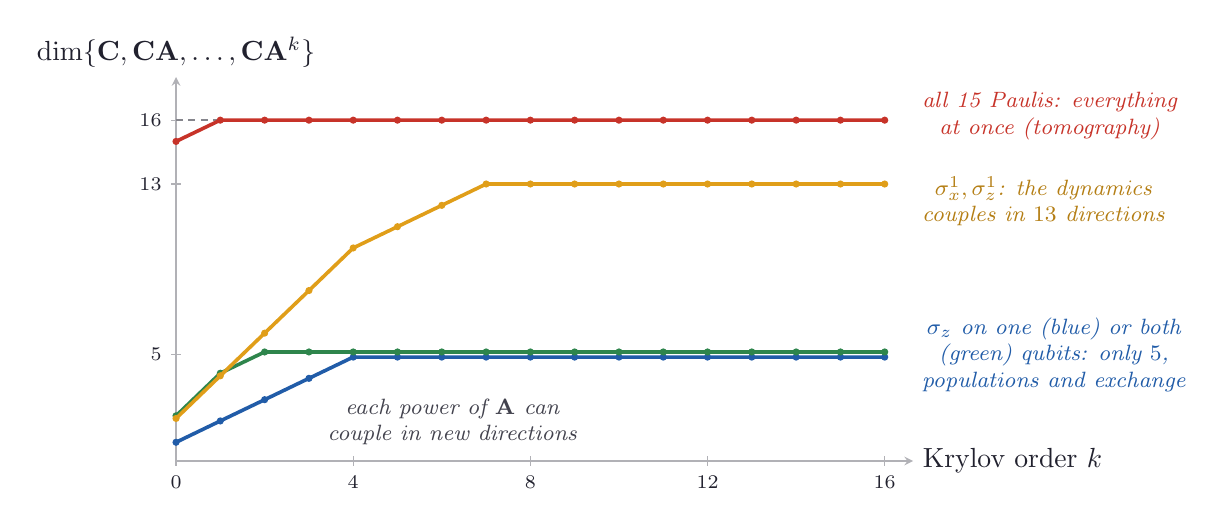
\begin{tikzpicture}[ink/.style={line width=0.9pt, ndInk}, faint/.style={line width=0.4pt, ndInk!35}, dashedink/.style={line width=0.5pt, ndInk!55, dash pattern=on 2.5pt off 2pt}, vec/.style={->, >=stealth, line width=1.2pt}, note/.style={font=\footnotesize\itshape, text=ndInk!85, align=center}, pointer/.style={->, >=stealth, line width=0.4pt, ndInk!60, shorten >=2pt, shorten <=1pt}, dot/.style={circle, fill=ndInk, inner sep=0pt, minimum size=3.4pt}, wash/.style={fill=ndSky, fill opacity=0.55}, every node/.style={text=ndInk}]
\definecolor{ndInk}{rgb}{0.13,0.13,0.18}
\definecolor{ndPaper}{rgb}{0.99,0.96,0.88}
\definecolor{ndSky}{rgb}{0.84,0.91,0.98}
\definecolor{ndRose}{rgb}{0.98,0.86,0.84}
\definecolor{ndBlue}{rgb}{0.13,0.36,0.66}
\definecolor{ndRed}{rgb}{0.78,0.20,0.16}
\definecolor{ndGold}{rgb}{0.88,0.62,0.10}
\definecolor{ndGreen}{rgb}{0.18,0.52,0.30}
\draw[faint, ->, >=stealth] (0.000,0.000) -- (9.360,0.000) node[right, text=ndInk] {Krylov order $k$};
\draw[faint, ->, >=stealth] (0.000,0.000) -- (0.000,4.876) node[above, text=ndInk] {$\dim\linspan\{\mathbf C,\mathbf C\mathbf A,\dots,\mathbf C\mathbf A^k\}$};
\draw[faint] (0.000,0.060) -- (0.000,-0.060) node[below, font=\scriptsize, text=ndInk] {$0$};
\draw[faint] (2.250,0.060) -- (2.250,-0.060) node[below, font=\scriptsize, text=ndInk] {$4$};
\draw[faint] (4.500,0.060) -- (4.500,-0.060) node[below, font=\scriptsize, text=ndInk] {$8$};
\draw[faint] (6.750,0.060) -- (6.750,-0.060) node[below, font=\scriptsize, text=ndInk] {$12$};
\draw[faint] (9.000,0.060) -- (9.000,-0.060) node[below, font=\scriptsize, text=ndInk] {$16$};
\draw[faint] (0.060,1.353) -- (-0.060,1.353) node[left, font=\scriptsize, text=ndInk] {$5$};
\draw[faint] (0.060,3.518) -- (-0.060,3.518) node[left, font=\scriptsize, text=ndInk] {$13$};
\draw[faint] (0.060,4.329) -- (-0.060,4.329) node[left, font=\scriptsize, text=ndInk] {$16$};
\draw[dashedink] (0.000,4.329) -- (9.000,4.329);
\draw[line width=1.3pt, ndBlue] (0.000,0.238) -- (0.562,0.509) -- (1.125,0.779) -- (1.688,1.050) -- (2.250,1.320) -- (2.812,1.320) -- (3.375,1.320) -- (3.938,1.320) -- (4.500,1.320) -- (5.062,1.320) -- (5.625,1.320) -- (6.188,1.320) -- (6.750,1.320) -- (7.312,1.320) -- (7.875,1.320) -- (8.438,1.320) -- (9.000,1.320);
\fill[ndBlue] (0.000,0.238) circle (1.3pt);
\fill[ndBlue] (0.562,0.509) circle (1.3pt);
\fill[ndBlue] (1.125,0.779) circle (1.3pt);
\fill[ndBlue] (1.688,1.050) circle (1.3pt);
\fill[ndBlue] (2.250,1.320) circle (1.3pt);
\fill[ndBlue] (2.812,1.320) circle (1.3pt);
\fill[ndBlue] (3.375,1.320) circle (1.3pt);
\fill[ndBlue] (3.938,1.320) circle (1.3pt);
\fill[ndBlue] (4.500,1.320) circle (1.3pt);
\fill[ndBlue] (5.062,1.320) circle (1.3pt);
\fill[ndBlue] (5.625,1.320) circle (1.3pt);
\fill[ndBlue] (6.188,1.320) circle (1.3pt);
\fill[ndBlue] (6.750,1.320) circle (1.3pt);
\fill[ndBlue] (7.312,1.320) circle (1.3pt);
\fill[ndBlue] (7.875,1.320) circle (1.3pt);
\fill[ndBlue] (8.438,1.320) circle (1.3pt);
\fill[ndBlue] (9.000,1.320) circle (1.3pt);
\draw[line width=1.3pt, ndGreen] (0.000,0.574) -- (0.562,1.115) -- (1.125,1.385) -- (1.688,1.385) -- (2.250,1.385) -- (2.812,1.385) -- (3.375,1.385) -- (3.938,1.385) -- (4.500,1.385) -- (5.062,1.385) -- (5.625,1.385) -- (6.188,1.385) -- (6.750,1.385) -- (7.312,1.385) -- (7.875,1.385) -- (8.438,1.385) -- (9.000,1.385);
\fill[ndGreen] (0.000,0.574) circle (1.3pt);
\fill[ndGreen] (0.562,1.115) circle (1.3pt);
\fill[ndGreen] (1.125,1.385) circle (1.3pt);
\fill[ndGreen] (1.688,1.385) circle (1.3pt);
\fill[ndGreen] (2.250,1.385) circle (1.3pt);
\fill[ndGreen] (2.812,1.385) circle (1.3pt);
\fill[ndGreen] (3.375,1.385) circle (1.3pt);
\fill[ndGreen] (3.938,1.385) circle (1.3pt);
\fill[ndGreen] (4.500,1.385) circle (1.3pt);
\fill[ndGreen] (5.062,1.385) circle (1.3pt);
\fill[ndGreen] (5.625,1.385) circle (1.3pt);
\fill[ndGreen] (6.188,1.385) circle (1.3pt);
\fill[ndGreen] (6.750,1.385) circle (1.3pt);
\fill[ndGreen] (7.312,1.385) circle (1.3pt);
\fill[ndGreen] (7.875,1.385) circle (1.3pt);
\fill[ndGreen] (8.438,1.385) circle (1.3pt);
\fill[ndGreen] (9.000,1.385) circle (1.3pt);
\draw[line width=1.3pt, ndGold] (0.000,0.541) -- (0.562,1.082) -- (1.125,1.624) -- (1.688,2.165) -- (2.250,2.706) -- (2.812,2.976) -- (3.375,3.247) -- (3.938,3.518) -- (4.500,3.518) -- (5.062,3.518) -- (5.625,3.518) -- (6.188,3.518) -- (6.750,3.518) -- (7.312,3.518) -- (7.875,3.518) -- (8.438,3.518) -- (9.000,3.518);
\fill[ndGold] (0.000,0.541) circle (1.3pt);
\fill[ndGold] (0.562,1.082) circle (1.3pt);
\fill[ndGold] (1.125,1.624) circle (1.3pt);
\fill[ndGold] (1.688,2.165) circle (1.3pt);
\fill[ndGold] (2.250,2.706) circle (1.3pt);
\fill[ndGold] (2.812,2.976) circle (1.3pt);
\fill[ndGold] (3.375,3.247) circle (1.3pt);
\fill[ndGold] (3.938,3.518) circle (1.3pt);
\fill[ndGold] (4.500,3.518) circle (1.3pt);
\fill[ndGold] (5.062,3.518) circle (1.3pt);
\fill[ndGold] (5.625,3.518) circle (1.3pt);
\fill[ndGold] (6.188,3.518) circle (1.3pt);
\fill[ndGold] (6.750,3.518) circle (1.3pt);
\fill[ndGold] (7.312,3.518) circle (1.3pt);
\fill[ndGold] (7.875,3.518) circle (1.3pt);
\fill[ndGold] (8.438,3.518) circle (1.3pt);
\fill[ndGold] (9.000,3.518) circle (1.3pt);
\draw[line width=1.3pt, ndRed] (0.000,4.059) -- (0.562,4.329) -- (1.125,4.329) -- (1.688,4.329) -- (2.250,4.329) -- (2.812,4.329) -- (3.375,4.329) -- (3.938,4.329) -- (4.500,4.329) -- (5.062,4.329) -- (5.625,4.329) -- (6.188,4.329) -- (6.750,4.329) -- (7.312,4.329) -- (7.875,4.329) -- (8.438,4.329) -- (9.000,4.329);
\fill[ndRed] (0.000,4.059) circle (1.3pt);
\fill[ndRed] (0.562,4.329) circle (1.3pt);
\fill[ndRed] (1.125,4.329) circle (1.3pt);
\fill[ndRed] (1.688,4.329) circle (1.3pt);
\fill[ndRed] (2.250,4.329) circle (1.3pt);
\fill[ndRed] (2.812,4.329) circle (1.3pt);
\fill[ndRed] (3.375,4.329) circle (1.3pt);
\fill[ndRed] (3.938,4.329) circle (1.3pt);
\fill[ndRed] (4.500,4.329) circle (1.3pt);
\fill[ndRed] (5.062,4.329) circle (1.3pt);
\fill[ndRed] (5.625,4.329) circle (1.3pt);
\fill[ndRed] (6.188,4.329) circle (1.3pt);
\fill[ndRed] (6.750,4.329) circle (1.3pt);
\fill[ndRed] (7.312,4.329) circle (1.3pt);
\fill[ndRed] (7.875,4.329) circle (1.3pt);
\fill[ndRed] (8.438,4.329) circle (1.3pt);
\fill[ndRed] (9.000,4.329) circle (1.3pt);
\node[note, anchor=west, text=ndRed] at (9.35,4.38) {all 15 Paulis: everything\\ at once (tomography)};
\node[note, anchor=west, text=ndGold!80!black] at (9.35,3.30) {$\sigma_x^1,\sigma_z^1$: the dynamics\\ couples in $13$ directions};
\node[note, anchor=west, text=ndBlue] at (9.35,1.35) {$\sigma_z$ on one (blue) or both\\ (green) qubits: only $5$,\\ populations and exchange};
\node[note, anchor=south west] at (1.800,0.081) {each power of $\mathbf A$ can\\ couple in new directions};
\end{tikzpicture}
}\end{center}}
\ona{\begin{figure}[H]\centering\resizebox{0.95\linewidth}{!}{% Generated by code/needham.py -- do not edit by hand.
\definecolor{qocA}{rgb}{0.00,0.45,0.70}
\definecolor{qocB}{rgb}{0.90,0.60,0.00}
\definecolor{qocC}{rgb}{0.00,0.62,0.45}
\definecolor{qocD}{rgb}{0.80,0.40,0.00}
\definecolor{qocE}{rgb}{0.80,0.60,0.70}
\definecolor{qocF}{rgb}{0.35,0.70,0.90}
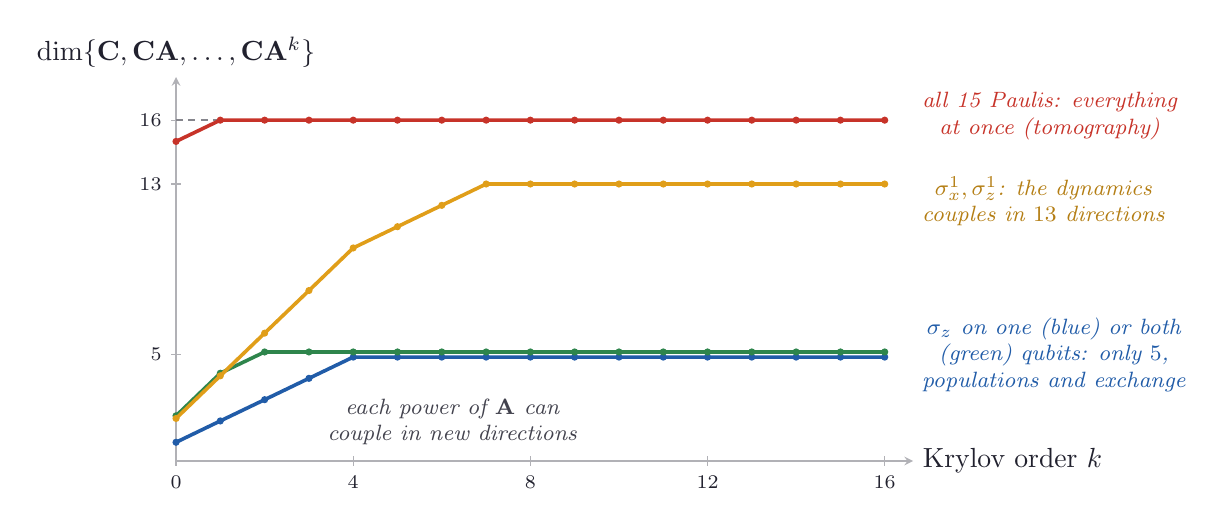
\begin{tikzpicture}[ink/.style={line width=0.9pt, ndInk}, faint/.style={line width=0.4pt, ndInk!35}, dashedink/.style={line width=0.5pt, ndInk!55, dash pattern=on 2.5pt off 2pt}, vec/.style={->, >=stealth, line width=1.2pt}, note/.style={font=\footnotesize\itshape, text=ndInk!85, align=center}, pointer/.style={->, >=stealth, line width=0.4pt, ndInk!60, shorten >=2pt, shorten <=1pt}, dot/.style={circle, fill=ndInk, inner sep=0pt, minimum size=3.4pt}, wash/.style={fill=ndSky, fill opacity=0.55}, every node/.style={text=ndInk}]
\definecolor{ndInk}{rgb}{0.13,0.13,0.18}
\definecolor{ndPaper}{rgb}{0.99,0.96,0.88}
\definecolor{ndSky}{rgb}{0.84,0.91,0.98}
\definecolor{ndRose}{rgb}{0.98,0.86,0.84}
\definecolor{ndBlue}{rgb}{0.13,0.36,0.66}
\definecolor{ndRed}{rgb}{0.78,0.20,0.16}
\definecolor{ndGold}{rgb}{0.88,0.62,0.10}
\definecolor{ndGreen}{rgb}{0.18,0.52,0.30}
\draw[faint, ->, >=stealth] (0.000,0.000) -- (9.360,0.000) node[right, text=ndInk] {Krylov order $k$};
\draw[faint, ->, >=stealth] (0.000,0.000) -- (0.000,4.876) node[above, text=ndInk] {$\dim\linspan\{\mathbf C,\mathbf C\mathbf A,\dots,\mathbf C\mathbf A^k\}$};
\draw[faint] (0.000,0.060) -- (0.000,-0.060) node[below, font=\scriptsize, text=ndInk] {$0$};
\draw[faint] (2.250,0.060) -- (2.250,-0.060) node[below, font=\scriptsize, text=ndInk] {$4$};
\draw[faint] (4.500,0.060) -- (4.500,-0.060) node[below, font=\scriptsize, text=ndInk] {$8$};
\draw[faint] (6.750,0.060) -- (6.750,-0.060) node[below, font=\scriptsize, text=ndInk] {$12$};
\draw[faint] (9.000,0.060) -- (9.000,-0.060) node[below, font=\scriptsize, text=ndInk] {$16$};
\draw[faint] (0.060,1.353) -- (-0.060,1.353) node[left, font=\scriptsize, text=ndInk] {$5$};
\draw[faint] (0.060,3.518) -- (-0.060,3.518) node[left, font=\scriptsize, text=ndInk] {$13$};
\draw[faint] (0.060,4.329) -- (-0.060,4.329) node[left, font=\scriptsize, text=ndInk] {$16$};
\draw[dashedink] (0.000,4.329) -- (9.000,4.329);
\draw[line width=1.3pt, ndBlue] (0.000,0.238) -- (0.562,0.509) -- (1.125,0.779) -- (1.688,1.050) -- (2.250,1.320) -- (2.812,1.320) -- (3.375,1.320) -- (3.938,1.320) -- (4.500,1.320) -- (5.062,1.320) -- (5.625,1.320) -- (6.188,1.320) -- (6.750,1.320) -- (7.312,1.320) -- (7.875,1.320) -- (8.438,1.320) -- (9.000,1.320);
\fill[ndBlue] (0.000,0.238) circle (1.3pt);
\fill[ndBlue] (0.562,0.509) circle (1.3pt);
\fill[ndBlue] (1.125,0.779) circle (1.3pt);
\fill[ndBlue] (1.688,1.050) circle (1.3pt);
\fill[ndBlue] (2.250,1.320) circle (1.3pt);
\fill[ndBlue] (2.812,1.320) circle (1.3pt);
\fill[ndBlue] (3.375,1.320) circle (1.3pt);
\fill[ndBlue] (3.938,1.320) circle (1.3pt);
\fill[ndBlue] (4.500,1.320) circle (1.3pt);
\fill[ndBlue] (5.062,1.320) circle (1.3pt);
\fill[ndBlue] (5.625,1.320) circle (1.3pt);
\fill[ndBlue] (6.188,1.320) circle (1.3pt);
\fill[ndBlue] (6.750,1.320) circle (1.3pt);
\fill[ndBlue] (7.312,1.320) circle (1.3pt);
\fill[ndBlue] (7.875,1.320) circle (1.3pt);
\fill[ndBlue] (8.438,1.320) circle (1.3pt);
\fill[ndBlue] (9.000,1.320) circle (1.3pt);
\draw[line width=1.3pt, ndGreen] (0.000,0.574) -- (0.562,1.115) -- (1.125,1.385) -- (1.688,1.385) -- (2.250,1.385) -- (2.812,1.385) -- (3.375,1.385) -- (3.938,1.385) -- (4.500,1.385) -- (5.062,1.385) -- (5.625,1.385) -- (6.188,1.385) -- (6.750,1.385) -- (7.312,1.385) -- (7.875,1.385) -- (8.438,1.385) -- (9.000,1.385);
\fill[ndGreen] (0.000,0.574) circle (1.3pt);
\fill[ndGreen] (0.562,1.115) circle (1.3pt);
\fill[ndGreen] (1.125,1.385) circle (1.3pt);
\fill[ndGreen] (1.688,1.385) circle (1.3pt);
\fill[ndGreen] (2.250,1.385) circle (1.3pt);
\fill[ndGreen] (2.812,1.385) circle (1.3pt);
\fill[ndGreen] (3.375,1.385) circle (1.3pt);
\fill[ndGreen] (3.938,1.385) circle (1.3pt);
\fill[ndGreen] (4.500,1.385) circle (1.3pt);
\fill[ndGreen] (5.062,1.385) circle (1.3pt);
\fill[ndGreen] (5.625,1.385) circle (1.3pt);
\fill[ndGreen] (6.188,1.385) circle (1.3pt);
\fill[ndGreen] (6.750,1.385) circle (1.3pt);
\fill[ndGreen] (7.312,1.385) circle (1.3pt);
\fill[ndGreen] (7.875,1.385) circle (1.3pt);
\fill[ndGreen] (8.438,1.385) circle (1.3pt);
\fill[ndGreen] (9.000,1.385) circle (1.3pt);
\draw[line width=1.3pt, ndGold] (0.000,0.541) -- (0.562,1.082) -- (1.125,1.624) -- (1.688,2.165) -- (2.250,2.706) -- (2.812,2.976) -- (3.375,3.247) -- (3.938,3.518) -- (4.500,3.518) -- (5.062,3.518) -- (5.625,3.518) -- (6.188,3.518) -- (6.750,3.518) -- (7.312,3.518) -- (7.875,3.518) -- (8.438,3.518) -- (9.000,3.518);
\fill[ndGold] (0.000,0.541) circle (1.3pt);
\fill[ndGold] (0.562,1.082) circle (1.3pt);
\fill[ndGold] (1.125,1.624) circle (1.3pt);
\fill[ndGold] (1.688,2.165) circle (1.3pt);
\fill[ndGold] (2.250,2.706) circle (1.3pt);
\fill[ndGold] (2.812,2.976) circle (1.3pt);
\fill[ndGold] (3.375,3.247) circle (1.3pt);
\fill[ndGold] (3.938,3.518) circle (1.3pt);
\fill[ndGold] (4.500,3.518) circle (1.3pt);
\fill[ndGold] (5.062,3.518) circle (1.3pt);
\fill[ndGold] (5.625,3.518) circle (1.3pt);
\fill[ndGold] (6.188,3.518) circle (1.3pt);
\fill[ndGold] (6.750,3.518) circle (1.3pt);
\fill[ndGold] (7.312,3.518) circle (1.3pt);
\fill[ndGold] (7.875,3.518) circle (1.3pt);
\fill[ndGold] (8.438,3.518) circle (1.3pt);
\fill[ndGold] (9.000,3.518) circle (1.3pt);
\draw[line width=1.3pt, ndRed] (0.000,4.059) -- (0.562,4.329) -- (1.125,4.329) -- (1.688,4.329) -- (2.250,4.329) -- (2.812,4.329) -- (3.375,4.329) -- (3.938,4.329) -- (4.500,4.329) -- (5.062,4.329) -- (5.625,4.329) -- (6.188,4.329) -- (6.750,4.329) -- (7.312,4.329) -- (7.875,4.329) -- (8.438,4.329) -- (9.000,4.329);
\fill[ndRed] (0.000,4.059) circle (1.3pt);
\fill[ndRed] (0.562,4.329) circle (1.3pt);
\fill[ndRed] (1.125,4.329) circle (1.3pt);
\fill[ndRed] (1.688,4.329) circle (1.3pt);
\fill[ndRed] (2.250,4.329) circle (1.3pt);
\fill[ndRed] (2.812,4.329) circle (1.3pt);
\fill[ndRed] (3.375,4.329) circle (1.3pt);
\fill[ndRed] (3.938,4.329) circle (1.3pt);
\fill[ndRed] (4.500,4.329) circle (1.3pt);
\fill[ndRed] (5.062,4.329) circle (1.3pt);
\fill[ndRed] (5.625,4.329) circle (1.3pt);
\fill[ndRed] (6.188,4.329) circle (1.3pt);
\fill[ndRed] (6.750,4.329) circle (1.3pt);
\fill[ndRed] (7.312,4.329) circle (1.3pt);
\fill[ndRed] (7.875,4.329) circle (1.3pt);
\fill[ndRed] (8.438,4.329) circle (1.3pt);
\fill[ndRed] (9.000,4.329) circle (1.3pt);
\node[note, anchor=west, text=ndRed] at (9.35,4.38) {all 15 Paulis: everything\\ at once (tomography)};
\node[note, anchor=west, text=ndGold!80!black] at (9.35,3.30) {$\sigma_x^1,\sigma_z^1$: the dynamics\\ couples in $13$ directions};
\node[note, anchor=west, text=ndBlue] at (9.35,1.35) {$\sigma_z$ on one (blue) or both\\ (green) qubits: only $5$,\\ populations and exchange};
\node[note, anchor=south west] at (1.800,0.081) {each power of $\mathbf A$ can\\ couple in new directions};
\end{tikzpicture}
}
\caption{Dimension of the observable subspace $\linspan\{\mathbf C,\mathbf C\mathbf A,\dots,\mathbf C\mathbf A^{k}\}$ of the (embedded, 16-dimensional) two-qubit model of Section~\ref{sec:ch04:example} for several readouts, Only an informationally complete readout observes the full state. Generated by \texttt{code/ch04\_observability.py}.}\label{fig:ch04:observability}\end{figure}}
\end{frame}

\begin{frame}\ft{The accessible set and the reduced system}
\ona{The size of the system matrices can be too large for efficient computation, however we only need the dynamics governing the evolution of the observables that are being measured. The dimensions of the system matrices can then be greatly reduced since it is likely that these evolutions do not couple all the matrices in $\mathcal{M}$ to those in the full basis. Inspired by control theory for classical nonlinear systems, an iterative procedure is used to find the finite set of generators $\mathcal M_{j}$ required to describe the dynamics of these observables,}
\onp{Only the part of $\mathcal F$ coupled to $\mathcal M$ by the dynamics matters:}
\begin{equation} \label{eq:ch04:accessible_set}
\begin{aligned}
    \mathcal M_{0} &= \mathcal{M},\qquad \mathcal M_{j} = [\mathcal M_{j-1}, \mathcal F] \cup \mathcal M_{j-1},\\
    [\mathcal M_{j-1}, \mathcal F] &= \{ F_{k}   \mid   \Tr[F^{\dagger}_k[F,F']] \neq 0,\ F \in \mathcal M_{j-1},\ F' \in \mathcal F  \}.
\end{aligned}
\end{equation}
\ona{This set is known as the \emph{accessible set} and is obtained when the procedure saturates, which will always occur since $\liesu[N]$ is finite-dimensional. Writing reduced vectors $\tilde{x}$ of dimension $\tilde n \leq n$ with reduced matrix ${\tilde{\mathbf{A}}} \in \R^{\tilde n \times \tilde n}$ allows us to rewrite \eqref{eq:ch04:BLDS} as $\dot{\tilde x} = \tilde{\mathbf{A}}\tilde{x}$. Here, only those parameters appearing in the reduced system can be identified. Practically, the consequence is that parameters associated with inaccessible degrees of freedom remain undetermined and irrelevant for the prediction of the measured outputs. In \eqref{eq:ch04:accessible_set}, $\mathcal F$ may, and in practice should, be replaced by the generators actually present in the Hamiltonian and the jump operators; commutators with the whole basis would make every set accessible after a few steps. The commutator rule captures the couplings due to the Hamiltonian. With dissipation, one reads all couplings, including those of the dissipator, off the non-zero pattern of $\mathbf A$: the accessible set consists of the components from which a path in this \emph{coupling graph} leads to a measured one. Observability of the full system requires that the accessible set is the whole basis $\mathcal F$. The converse holds for generic parameters, but not always: exact relations between the couplings can hide combinations of components even inside the accessible set, so that the rank test of $\OM^{(\mathrm{lin})}$ has the last word (Figure~\ref{fig:ch04:coupling}).}
\onp{\begin{itemize}
    \item Saturates in finitely many steps; gives the reduced system $\dot{\tilde x}=\tilde{\mathbf A}\tilde x$.
    \item Parameters supported outside the accessible set are \alert{not identifiable} and irrelevant for predicting the data.
    \item Full observability needs the accessible set to be all of $\mathcal F$; the rank of $\OM$ has the last word.
\end{itemize}}
\end{frame}

\begin{frame}\ft{The coupling graph}
\ona{Figure~\ref{fig:ch04:coupling} computes the accessible set of the two-qubit example of Section~\ref{sec:ch04:example} as a search on its coupling graph. The graph falls into two sectors that never exchange information: the populations together with the exchange components, and the single-qubit coherences. Measuring $\sigma_z^1$, seven components have a path to the measured one, but $\OM^{(\mathrm{lin})}$ has rank $5$ only, because the four exchange components enter only through the combinations $XX+YY$ and $XY-YX$. Up to constants, these are the exchange operator $\sigma_+^1\sigma_-^2+\sigma_-^1\sigma_+^2$ and the excitation current between the qubits. This is the gap between the graph-based accessible set and the rank test. The component along $ZZ$ is driven by $ZI$ and $IZ$, but never drives them, so it stays invisible. Adding $\sigma_x^1$ opens the second sector, and $15$ components can reach the readout, but the rank is $13$; only a richer readout observes everything (Figure~\ref{fig:ch04:observability}).}
\ona{\begin{figure}[H]\centering
\resizebox{\linewidth}{!}{% Generated by code/needham.py -- do not edit by hand.
\definecolor{qocA}{rgb}{0.00,0.45,0.70}
\definecolor{qocB}{rgb}{0.90,0.60,0.00}
\definecolor{qocC}{rgb}{0.00,0.62,0.45}
\definecolor{qocD}{rgb}{0.80,0.40,0.00}
\definecolor{qocE}{rgb}{0.80,0.60,0.70}
\definecolor{qocF}{rgb}{0.35,0.70,0.90}
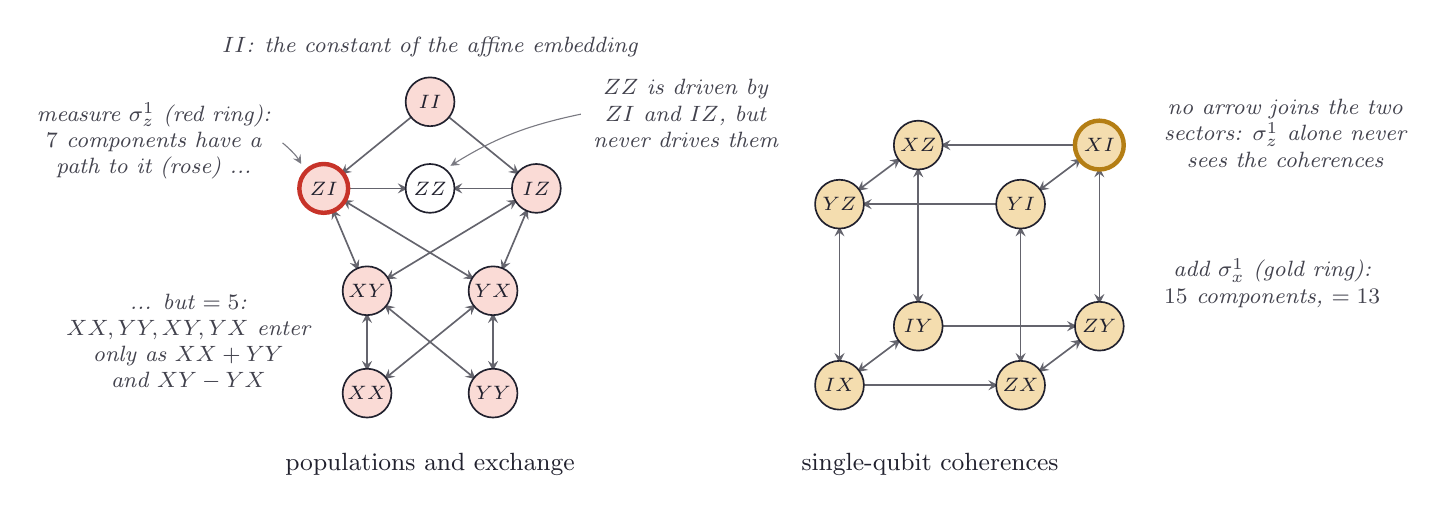
\begin{tikzpicture}[ink/.style={line width=0.9pt, ndInk}, faint/.style={line width=0.4pt, ndInk!35}, dashedink/.style={line width=0.5pt, ndInk!55, dash pattern=on 2.5pt off 2pt}, vec/.style={->, >=stealth, line width=1.2pt}, note/.style={font=\footnotesize\itshape, text=ndInk!85, align=center}, pointer/.style={->, >=stealth, line width=0.4pt, ndInk!60, shorten >=2pt, shorten <=1pt}, dot/.style={circle, fill=ndInk, inner sep=0pt, minimum size=3.4pt}, wash/.style={fill=ndSky, fill opacity=0.55}, every node/.style={text=ndInk}]
\definecolor{ndInk}{rgb}{0.13,0.13,0.18}
\definecolor{ndPaper}{rgb}{0.99,0.96,0.88}
\definecolor{ndSky}{rgb}{0.84,0.91,0.98}
\definecolor{ndRose}{rgb}{0.98,0.86,0.84}
\definecolor{ndBlue}{rgb}{0.13,0.36,0.66}
\definecolor{ndRed}{rgb}{0.78,0.20,0.16}
\definecolor{ndGold}{rgb}{0.88,0.62,0.10}
\definecolor{ndGreen}{rgb}{0.18,0.52,0.30}
\draw[->, >=stealth, line width=0.6pt, ndInk!70, shorten <=8pt, shorten >=8pt] (0.00,2.70) -- (1.35,1.60);
\draw[->, >=stealth, line width=0.6pt, ndInk!70, shorten <=8pt, shorten >=8pt] (0.00,2.70) -- (-1.35,1.60);
\draw[<->, >=stealth, line width=0.6pt, ndInk!70, shorten <=8pt, shorten >=8pt] (5.20,-0.90) -- (6.20,-0.15);
\draw[<->, >=stealth, line width=0.6pt, ndInk!70, shorten <=8pt, shorten >=8pt] (5.20,-0.90) -- (5.20,1.40);
\draw[->, >=stealth, line width=0.6pt, ndInk!70, shorten <=8pt, shorten >=8pt] (5.20,-0.90) -- (7.50,-0.90);
\draw[<->, >=stealth, line width=0.6pt, ndInk!70, shorten <=8pt, shorten >=8pt] (6.20,-0.15) -- (6.20,2.15);
\draw[->, >=stealth, line width=0.6pt, ndInk!70, shorten <=8pt, shorten >=8pt] (6.20,-0.15) -- (8.50,-0.15);
\draw[<->, >=stealth, line width=0.6pt, ndInk!70, shorten <=8pt, shorten >=8pt] (1.35,1.60) -- (-0.80,0.30);
\draw[<->, >=stealth, line width=0.6pt, ndInk!70, shorten <=8pt, shorten >=8pt] (1.35,1.60) -- (0.80,0.30);
\draw[->, >=stealth, line width=0.6pt, ndInk!70, shorten <=8pt, shorten >=8pt] (1.35,1.60) -- (0.00,1.60);
\draw[->, >=stealth, line width=0.6pt, ndInk!70, shorten <=8pt, shorten >=8pt] (8.50,2.15) -- (6.20,2.15);
\draw[<->, >=stealth, line width=0.6pt, ndInk!70, shorten <=8pt, shorten >=8pt] (8.50,2.15) -- (7.50,1.40);
\draw[<->, >=stealth, line width=0.6pt, ndInk!70, shorten <=8pt, shorten >=8pt] (8.50,2.15) -- (8.50,-0.15);
\draw[<->, >=stealth, line width=0.6pt, ndInk!70, shorten <=8pt, shorten >=8pt] (-0.80,-1.00) -- (-0.80,0.30);
\draw[<->, >=stealth, line width=0.6pt, ndInk!70, shorten <=8pt, shorten >=8pt] (-0.80,-1.00) -- (0.80,0.30);
\draw[<->, >=stealth, line width=0.6pt, ndInk!70, shorten <=8pt, shorten >=8pt] (-0.80,0.30) -- (0.80,-1.00);
\draw[<->, >=stealth, line width=0.6pt, ndInk!70, shorten <=8pt, shorten >=8pt] (-0.80,0.30) -- (-1.35,1.60);
\draw[<->, >=stealth, line width=0.6pt, ndInk!70, shorten <=8pt, shorten >=8pt] (6.20,2.15) -- (5.20,1.40);
\draw[->, >=stealth, line width=0.6pt, ndInk!70, shorten <=8pt, shorten >=8pt] (7.50,1.40) -- (5.20,1.40);
\draw[<->, >=stealth, line width=0.6pt, ndInk!70, shorten <=8pt, shorten >=8pt] (7.50,1.40) -- (7.50,-0.90);
\draw[<->, >=stealth, line width=0.6pt, ndInk!70, shorten <=8pt, shorten >=8pt] (0.80,0.30) -- (0.80,-1.00);
\draw[<->, >=stealth, line width=0.6pt, ndInk!70, shorten <=8pt, shorten >=8pt] (0.80,0.30) -- (-1.35,1.60);
\draw[->, >=stealth, line width=0.6pt, ndInk!70, shorten <=8pt, shorten >=8pt] (-1.35,1.60) -- (0.00,1.60);
\draw[<->, >=stealth, line width=0.6pt, ndInk!70, shorten <=8pt, shorten >=8pt] (7.50,-0.90) -- (8.50,-0.15);
\node[circle, draw=ndInk, line width=0.6pt, fill=ndGold!35, inner sep=0pt, minimum size=0.62cm, font=\scriptsize] at (5.20,-0.90) {$IX$};
\node[circle, draw=ndInk, line width=0.6pt, fill=ndGold!35, inner sep=0pt, minimum size=0.62cm, font=\scriptsize] at (6.20,-0.15) {$IY$};
\node[circle, draw=ndInk, line width=0.6pt, fill=ndRose, inner sep=0pt, minimum size=0.62cm, font=\scriptsize] at (1.35,1.60) {$IZ$};
\node[circle, draw=ndGold!80!black, line width=1.6pt, fill=ndGold!35, inner sep=0pt, minimum size=0.62cm, font=\scriptsize] at (8.50,2.15) {$XI$};
\node[circle, draw=ndInk, line width=0.6pt, fill=ndRose, inner sep=0pt, minimum size=0.62cm, font=\scriptsize] at (-0.80,-1.00) {$XX$};
\node[circle, draw=ndInk, line width=0.6pt, fill=ndRose, inner sep=0pt, minimum size=0.62cm, font=\scriptsize] at (-0.80,0.30) {$XY$};
\node[circle, draw=ndInk, line width=0.6pt, fill=ndGold!35, inner sep=0pt, minimum size=0.62cm, font=\scriptsize] at (6.20,2.15) {$XZ$};
\node[circle, draw=ndInk, line width=0.6pt, fill=ndGold!35, inner sep=0pt, minimum size=0.62cm, font=\scriptsize] at (7.50,1.40) {$YI$};
\node[circle, draw=ndInk, line width=0.6pt, fill=ndRose, inner sep=0pt, minimum size=0.62cm, font=\scriptsize] at (0.80,0.30) {$YX$};
\node[circle, draw=ndInk, line width=0.6pt, fill=ndRose, inner sep=0pt, minimum size=0.62cm, font=\scriptsize] at (0.80,-1.00) {$YY$};
\node[circle, draw=ndInk, line width=0.6pt, fill=ndGold!35, inner sep=0pt, minimum size=0.62cm, font=\scriptsize] at (5.20,1.40) {$YZ$};
\node[circle, draw=ndRed, line width=1.6pt, fill=ndRose, inner sep=0pt, minimum size=0.62cm, font=\scriptsize] at (-1.35,1.60) {$ZI$};
\node[circle, draw=ndInk, line width=0.6pt, fill=ndGold!35, inner sep=0pt, minimum size=0.62cm, font=\scriptsize] at (7.50,-0.90) {$ZX$};
\node[circle, draw=ndInk, line width=0.6pt, fill=ndGold!35, inner sep=0pt, minimum size=0.62cm, font=\scriptsize] at (8.50,-0.15) {$ZY$};
\node[circle, draw=ndInk, line width=0.6pt, fill=white, inner sep=0pt, minimum size=0.62cm, font=\scriptsize] at (0.00,1.60) {$ZZ$};
\node[circle, draw=ndInk, line width=0.6pt, fill=ndRose, inner sep=0pt, minimum size=0.62cm, font=\scriptsize] at (0.00,2.70) {$II$};
\node[font=\small] at (0.0,-1.9) {populations and exchange};
\node[font=\small] at (6.35,-1.9) {single-qubit coherences};
\node[note, anchor=east] (a) at (-1.9,2.2) {measure $\sigma_z^1$ (red ring):\\ $7$ components have a\\ path to it (rose) ...};
\draw[pointer] (a.east) to[bend left=10] (-1.60,1.85);
\node[note, anchor=east] at (-1.4,-0.35) {... but $\rank\OM=5$:\\ $XX,YY,XY,YX$ enter\\ only as $XX+YY$\\ and $XY-YX$};
\node[note, anchor=south] at (0.0,3.15) {$II$: the constant of the affine embedding};
\node[note, anchor=west] (zz) at (1.95,2.55) {$ZZ$ is driven by\\ $ZI$ and $IZ$, but\\ never drives them};
\draw[pointer] (zz.west) to[bend right=10] (0.20,1.85);
\node[note, anchor=west] at (9.2,2.3) {no arrow joins the two\\ sectors: $\sigma_z^1$ alone never\\ sees the coherences};
\node[note, anchor=west] at (9.2,0.4) {add $\sigma_x^1$ (gold ring):\\ $15$ components, $\rank\OM=13$};
\end{tikzpicture}
}
\caption{The coupling graph of the two-qubit example: one vertex per component of the coherence vector, labelled by its Pauli string, and $II$ for the constant of the affine embedding, with an arrow from $F$ to $F'$ whenever the component along $F$ appears in the equation for the component along $F'$. Rose: the components with a path to the measured $\sigma_z^1$ (red ring). Gold: the sector reached by adding $\sigma_x^1$ (gold ring). Generated by \texttt{code/ch04\_coupling.py}.}\label{fig:ch04:coupling}
\end{figure}}
\onp{\begin{center}\resizebox{\linewidth}{!}{% Generated by code/needham.py -- do not edit by hand.
\definecolor{qocA}{rgb}{0.00,0.45,0.70}
\definecolor{qocB}{rgb}{0.90,0.60,0.00}
\definecolor{qocC}{rgb}{0.00,0.62,0.45}
\definecolor{qocD}{rgb}{0.80,0.40,0.00}
\definecolor{qocE}{rgb}{0.80,0.60,0.70}
\definecolor{qocF}{rgb}{0.35,0.70,0.90}
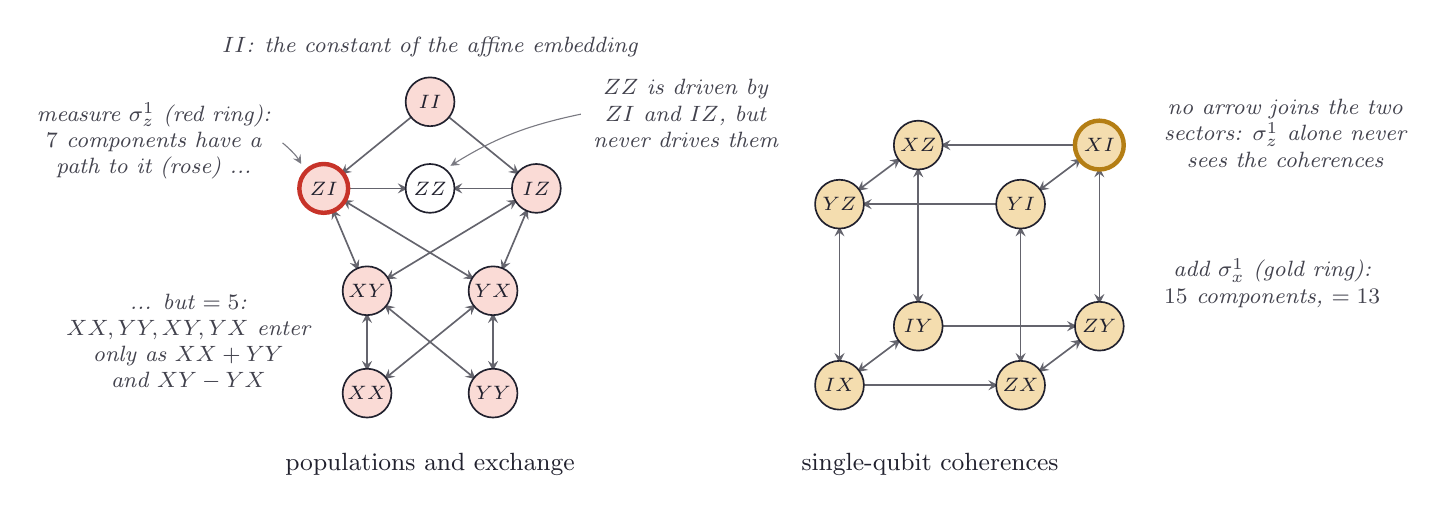
\begin{tikzpicture}[ink/.style={line width=0.9pt, ndInk}, faint/.style={line width=0.4pt, ndInk!35}, dashedink/.style={line width=0.5pt, ndInk!55, dash pattern=on 2.5pt off 2pt}, vec/.style={->, >=stealth, line width=1.2pt}, note/.style={font=\footnotesize\itshape, text=ndInk!85, align=center}, pointer/.style={->, >=stealth, line width=0.4pt, ndInk!60, shorten >=2pt, shorten <=1pt}, dot/.style={circle, fill=ndInk, inner sep=0pt, minimum size=3.4pt}, wash/.style={fill=ndSky, fill opacity=0.55}, every node/.style={text=ndInk}]
\definecolor{ndInk}{rgb}{0.13,0.13,0.18}
\definecolor{ndPaper}{rgb}{0.99,0.96,0.88}
\definecolor{ndSky}{rgb}{0.84,0.91,0.98}
\definecolor{ndRose}{rgb}{0.98,0.86,0.84}
\definecolor{ndBlue}{rgb}{0.13,0.36,0.66}
\definecolor{ndRed}{rgb}{0.78,0.20,0.16}
\definecolor{ndGold}{rgb}{0.88,0.62,0.10}
\definecolor{ndGreen}{rgb}{0.18,0.52,0.30}
\draw[->, >=stealth, line width=0.6pt, ndInk!70, shorten <=8pt, shorten >=8pt] (0.00,2.70) -- (1.35,1.60);
\draw[->, >=stealth, line width=0.6pt, ndInk!70, shorten <=8pt, shorten >=8pt] (0.00,2.70) -- (-1.35,1.60);
\draw[<->, >=stealth, line width=0.6pt, ndInk!70, shorten <=8pt, shorten >=8pt] (5.20,-0.90) -- (6.20,-0.15);
\draw[<->, >=stealth, line width=0.6pt, ndInk!70, shorten <=8pt, shorten >=8pt] (5.20,-0.90) -- (5.20,1.40);
\draw[->, >=stealth, line width=0.6pt, ndInk!70, shorten <=8pt, shorten >=8pt] (5.20,-0.90) -- (7.50,-0.90);
\draw[<->, >=stealth, line width=0.6pt, ndInk!70, shorten <=8pt, shorten >=8pt] (6.20,-0.15) -- (6.20,2.15);
\draw[->, >=stealth, line width=0.6pt, ndInk!70, shorten <=8pt, shorten >=8pt] (6.20,-0.15) -- (8.50,-0.15);
\draw[<->, >=stealth, line width=0.6pt, ndInk!70, shorten <=8pt, shorten >=8pt] (1.35,1.60) -- (-0.80,0.30);
\draw[<->, >=stealth, line width=0.6pt, ndInk!70, shorten <=8pt, shorten >=8pt] (1.35,1.60) -- (0.80,0.30);
\draw[->, >=stealth, line width=0.6pt, ndInk!70, shorten <=8pt, shorten >=8pt] (1.35,1.60) -- (0.00,1.60);
\draw[->, >=stealth, line width=0.6pt, ndInk!70, shorten <=8pt, shorten >=8pt] (8.50,2.15) -- (6.20,2.15);
\draw[<->, >=stealth, line width=0.6pt, ndInk!70, shorten <=8pt, shorten >=8pt] (8.50,2.15) -- (7.50,1.40);
\draw[<->, >=stealth, line width=0.6pt, ndInk!70, shorten <=8pt, shorten >=8pt] (8.50,2.15) -- (8.50,-0.15);
\draw[<->, >=stealth, line width=0.6pt, ndInk!70, shorten <=8pt, shorten >=8pt] (-0.80,-1.00) -- (-0.80,0.30);
\draw[<->, >=stealth, line width=0.6pt, ndInk!70, shorten <=8pt, shorten >=8pt] (-0.80,-1.00) -- (0.80,0.30);
\draw[<->, >=stealth, line width=0.6pt, ndInk!70, shorten <=8pt, shorten >=8pt] (-0.80,0.30) -- (0.80,-1.00);
\draw[<->, >=stealth, line width=0.6pt, ndInk!70, shorten <=8pt, shorten >=8pt] (-0.80,0.30) -- (-1.35,1.60);
\draw[<->, >=stealth, line width=0.6pt, ndInk!70, shorten <=8pt, shorten >=8pt] (6.20,2.15) -- (5.20,1.40);
\draw[->, >=stealth, line width=0.6pt, ndInk!70, shorten <=8pt, shorten >=8pt] (7.50,1.40) -- (5.20,1.40);
\draw[<->, >=stealth, line width=0.6pt, ndInk!70, shorten <=8pt, shorten >=8pt] (7.50,1.40) -- (7.50,-0.90);
\draw[<->, >=stealth, line width=0.6pt, ndInk!70, shorten <=8pt, shorten >=8pt] (0.80,0.30) -- (0.80,-1.00);
\draw[<->, >=stealth, line width=0.6pt, ndInk!70, shorten <=8pt, shorten >=8pt] (0.80,0.30) -- (-1.35,1.60);
\draw[->, >=stealth, line width=0.6pt, ndInk!70, shorten <=8pt, shorten >=8pt] (-1.35,1.60) -- (0.00,1.60);
\draw[<->, >=stealth, line width=0.6pt, ndInk!70, shorten <=8pt, shorten >=8pt] (7.50,-0.90) -- (8.50,-0.15);
\node[circle, draw=ndInk, line width=0.6pt, fill=ndGold!35, inner sep=0pt, minimum size=0.62cm, font=\scriptsize] at (5.20,-0.90) {$IX$};
\node[circle, draw=ndInk, line width=0.6pt, fill=ndGold!35, inner sep=0pt, minimum size=0.62cm, font=\scriptsize] at (6.20,-0.15) {$IY$};
\node[circle, draw=ndInk, line width=0.6pt, fill=ndRose, inner sep=0pt, minimum size=0.62cm, font=\scriptsize] at (1.35,1.60) {$IZ$};
\node[circle, draw=ndGold!80!black, line width=1.6pt, fill=ndGold!35, inner sep=0pt, minimum size=0.62cm, font=\scriptsize] at (8.50,2.15) {$XI$};
\node[circle, draw=ndInk, line width=0.6pt, fill=ndRose, inner sep=0pt, minimum size=0.62cm, font=\scriptsize] at (-0.80,-1.00) {$XX$};
\node[circle, draw=ndInk, line width=0.6pt, fill=ndRose, inner sep=0pt, minimum size=0.62cm, font=\scriptsize] at (-0.80,0.30) {$XY$};
\node[circle, draw=ndInk, line width=0.6pt, fill=ndGold!35, inner sep=0pt, minimum size=0.62cm, font=\scriptsize] at (6.20,2.15) {$XZ$};
\node[circle, draw=ndInk, line width=0.6pt, fill=ndGold!35, inner sep=0pt, minimum size=0.62cm, font=\scriptsize] at (7.50,1.40) {$YI$};
\node[circle, draw=ndInk, line width=0.6pt, fill=ndRose, inner sep=0pt, minimum size=0.62cm, font=\scriptsize] at (0.80,0.30) {$YX$};
\node[circle, draw=ndInk, line width=0.6pt, fill=ndRose, inner sep=0pt, minimum size=0.62cm, font=\scriptsize] at (0.80,-1.00) {$YY$};
\node[circle, draw=ndInk, line width=0.6pt, fill=ndGold!35, inner sep=0pt, minimum size=0.62cm, font=\scriptsize] at (5.20,1.40) {$YZ$};
\node[circle, draw=ndRed, line width=1.6pt, fill=ndRose, inner sep=0pt, minimum size=0.62cm, font=\scriptsize] at (-1.35,1.60) {$ZI$};
\node[circle, draw=ndInk, line width=0.6pt, fill=ndGold!35, inner sep=0pt, minimum size=0.62cm, font=\scriptsize] at (7.50,-0.90) {$ZX$};
\node[circle, draw=ndInk, line width=0.6pt, fill=ndGold!35, inner sep=0pt, minimum size=0.62cm, font=\scriptsize] at (8.50,-0.15) {$ZY$};
\node[circle, draw=ndInk, line width=0.6pt, fill=white, inner sep=0pt, minimum size=0.62cm, font=\scriptsize] at (0.00,1.60) {$ZZ$};
\node[circle, draw=ndInk, line width=0.6pt, fill=ndRose, inner sep=0pt, minimum size=0.62cm, font=\scriptsize] at (0.00,2.70) {$II$};
\node[font=\small] at (0.0,-1.9) {populations and exchange};
\node[font=\small] at (6.35,-1.9) {single-qubit coherences};
\node[note, anchor=east] (a) at (-1.9,2.2) {measure $\sigma_z^1$ (red ring):\\ $7$ components have a\\ path to it (rose) ...};
\draw[pointer] (a.east) to[bend left=10] (-1.60,1.85);
\node[note, anchor=east] at (-1.4,-0.35) {... but $\rank\OM=5$:\\ $XX,YY,XY,YX$ enter\\ only as $XX+YY$\\ and $XY-YX$};
\node[note, anchor=south] at (0.0,3.15) {$II$: the constant of the affine embedding};
\node[note, anchor=west] (zz) at (1.95,2.55) {$ZZ$ is driven by\\ $ZI$ and $IZ$, but\\ never drives them};
\draw[pointer] (zz.west) to[bend right=10] (0.20,1.85);
\node[note, anchor=west] at (9.2,2.3) {no arrow joins the two\\ sectors: $\sigma_z^1$ alone never\\ sees the coherences};
\node[note, anchor=west] at (9.2,0.4) {add $\sigma_x^1$ (gold ring):\\ $15$ components, $\rank\OM=13$};
\end{tikzpicture}
}\end{center}
Graph search: an upper bound. $\sigma_z^1$: $7$ reachable, $\rank\OM=5$.}
\end{frame}

\begin{frame}\ft{Example: a damped qubit}
\ona{For a single qubit with $H=-\frac\omega2\sigma_z$, so that $\ket0$ is the ground state, amplitude damping towards $\ket0$ at the rate $\gamma_1$ and dephasing at the rate $\gamma_\phi$, the coherence vector is the Bloch vector scaled by $1/\sqrt2$, and \eqref{eq:ch04:BLDS} gives the Bloch equations \eqref{eq:ch03:bloch-open} of \Chap~\ref{C.Open}, $\dot x=\omega y-x/T_2$, $\dot y=-\omega x-y/T_2$, $\dot z=-(z-1)/T_1$, with $1/T_1=\gamma_1$ and $1/T_2=\gamma_1/2+\gamma_\phi$. The transverse block $(x,y)$ and the longitudinal block $(z,1)$ decouple. Measuring $\sigma_z$ alone observes only the longitudinal block; measuring $\sigma_x$ alone observes the transverse block, since the rotation by $\omega$ feeds $y$ into $x$; both together observe everything. Figure~\ref{fig:ch04:singular} shows the singular values of $\OM^{(\mathrm{lin})}$ in the three cases. The smallest nonzero singular value, here $s_4\approx0.2$, quantifies how well-conditioned the inversion from data to state is; \Chap~\ref{C.SampleComplexity} turns this into a statement about the number of measurement shots needed.}
\onp{\begin{itemize}
    \item $\dot x=\omega y-x/T_2$, $\dot y=-\omega x-y/T_2$, $\dot z=-(z-1)/T_1$: two decoupled blocks.
    \item $\sigma_z$ alone sees $(z,1)$; $\sigma_x$ alone sees $(x,y)$ thanks to the rotation; both see all.
    \item Small singular values of $\Obsv$ $\Rightarrow$ ill-conditioned $\Rightarrow$ many shots (\Chap~\ref{C.SampleComplexity}).
\end{itemize}
\begin{center}\resizebox{!}{0.45\textheight}{% Generated by code/needham.py -- do not edit by hand.
\definecolor{qocA}{rgb}{0.00,0.45,0.70}
\definecolor{qocB}{rgb}{0.90,0.60,0.00}
\definecolor{qocC}{rgb}{0.00,0.62,0.45}
\definecolor{qocD}{rgb}{0.80,0.40,0.00}
\definecolor{qocE}{rgb}{0.80,0.60,0.70}
\definecolor{qocF}{rgb}{0.35,0.70,0.90}
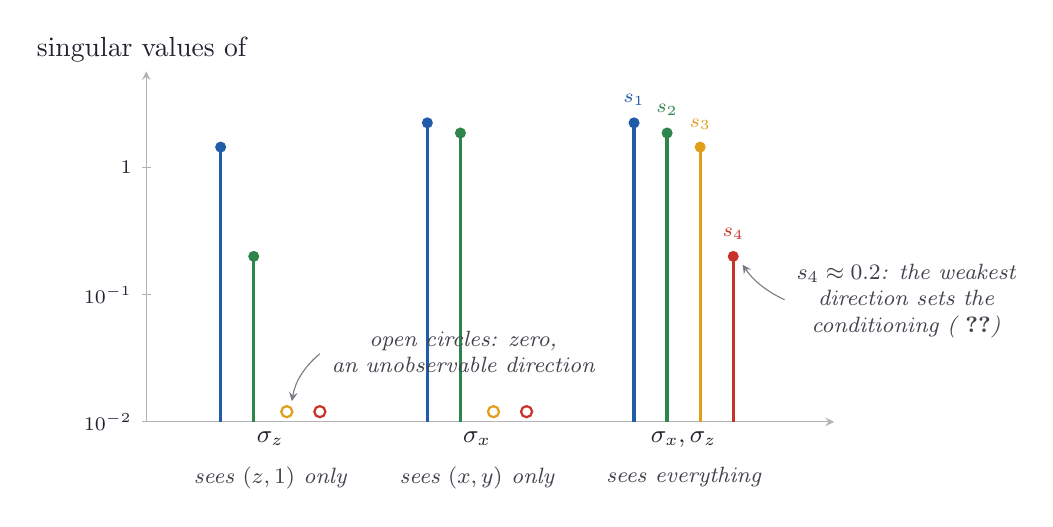
\begin{tikzpicture}[ink/.style={line width=0.9pt, ndInk}, faint/.style={line width=0.4pt, ndInk!35}, dashedink/.style={line width=0.5pt, ndInk!55, dash pattern=on 2.5pt off 2pt}, vec/.style={->, >=stealth, line width=1.2pt}, note/.style={font=\footnotesize\itshape, text=ndInk!85, align=center}, pointer/.style={->, >=stealth, line width=0.4pt, ndInk!60, shorten >=2pt, shorten <=1pt}, dot/.style={circle, fill=ndInk, inner sep=0pt, minimum size=3.4pt}, wash/.style={fill=ndSky, fill opacity=0.55}, every node/.style={text=ndInk}]
\definecolor{ndInk}{rgb}{0.13,0.13,0.18}
\definecolor{ndPaper}{rgb}{0.99,0.96,0.88}
\definecolor{ndSky}{rgb}{0.84,0.91,0.98}
\definecolor{ndRose}{rgb}{0.98,0.86,0.84}
\definecolor{ndBlue}{rgb}{0.13,0.36,0.66}
\definecolor{ndRed}{rgb}{0.78,0.20,0.16}
\definecolor{ndGold}{rgb}{0.88,0.62,0.10}
\definecolor{ndGreen}{rgb}{0.18,0.52,0.30}
\draw[faint, ->, >=stealth] (0.000,0.000) -- (8.736,0.000) node[right, text=ndInk] {};
\draw[faint, ->, >=stealth] (0.000,0.000) -- (0.000,4.452) node[above, text=ndInk] {singular values of $\Obsv$};
\draw[faint] (0.060,0.000) -- (-0.060,0.000) node[left, font=\scriptsize, text=ndInk] {$10^{-2}$};
\draw[faint] (0.060,1.615) -- (-0.060,1.615) node[left, font=\scriptsize, text=ndInk] {$10^{-1}$};
\draw[faint] (0.060,3.231) -- (-0.060,3.231) node[left, font=\scriptsize, text=ndInk] {$1$};
\draw[line width=1.2pt, ndBlue] (0.945,0.000) -- (0.945,3.489);
\fill[ndBlue] (0.945,3.489) circle (2pt);
\draw[line width=1.2pt, ndGreen] (1.365,0.000) -- (1.365,2.101);
\fill[ndGreen] (1.365,2.101) circle (2pt);
\draw[line width=0.8pt, ndGold, fill=white] (1.785,0.129) circle (2pt);
\draw[line width=0.8pt, ndRed, fill=white] (2.205,0.129) circle (2pt);
\node[below, font=\small] at (1.575,0.000) {$\sigma_z$};
\node[note, below] at (1.575,-0.450) {sees $(z,1)$ only};
\draw[line width=1.2pt, ndBlue] (3.570,0.000) -- (3.570,3.797);
\fill[ndBlue] (3.570,3.797) circle (2pt);
\draw[line width=1.2pt, ndGreen] (3.990,0.000) -- (3.990,3.668);
\fill[ndGreen] (3.990,3.668) circle (2pt);
\draw[line width=0.8pt, ndGold, fill=white] (4.410,0.129) circle (2pt);
\draw[line width=0.8pt, ndRed, fill=white] (4.830,0.129) circle (2pt);
\node[below, font=\small] at (4.200,0.000) {$\sigma_x$};
\node[note, below] at (4.200,-0.450) {sees $(x,y)$ only};
\draw[line width=1.2pt, ndBlue] (6.195,0.000) -- (6.195,3.797);
\fill[ndBlue] (6.195,3.797) circle (2pt);
\draw[line width=1.2pt, ndGreen] (6.615,0.000) -- (6.615,3.668);
\fill[ndGreen] (6.615,3.668) circle (2pt);
\draw[line width=1.2pt, ndGold] (7.035,0.000) -- (7.035,3.489);
\fill[ndGold] (7.035,3.489) circle (2pt);
\draw[line width=1.2pt, ndRed] (7.455,0.000) -- (7.455,2.101);
\fill[ndRed] (7.455,2.101) circle (2pt);
\node[below, font=\small] at (6.825,0.000) {$\sigma_x,\sigma_z$};
\node[note, below] at (6.825,-0.450) {sees everything};
\node[note, anchor=west] (z) at (2.231,0.888) {open circles: zero,\\ an unobservable direction};
\draw[pointer] (z.west) to[bend right=20] (1.838,0.194);
\node[note, anchor=west] (s) at (8.138,1.535) {$s_4\approx0.2$: the weakest\\ direction sets the\\ conditioning (\Chap~\ref{C.SampleComplexity})};
\draw[pointer] (s.west) to[bend left=15] (7.534,2.053);
\node[font=\scriptsize, text=ndBlue] at (6.195,4.087) {$s_1$};
\node[font=\scriptsize, text=ndGreen] at (6.615,3.958) {$s_2$};
\node[font=\scriptsize, text=ndGold] at (7.035,3.779) {$s_3$};
\node[font=\scriptsize, text=ndRed] at (7.455,2.392) {$s_4$};
\end{tikzpicture}
}\end{center}}
\ona{\begin{figure}[H]\centering\resizebox{0.9\linewidth}{!}{% Generated by code/needham.py -- do not edit by hand.
\definecolor{qocA}{rgb}{0.00,0.45,0.70}
\definecolor{qocB}{rgb}{0.90,0.60,0.00}
\definecolor{qocC}{rgb}{0.00,0.62,0.45}
\definecolor{qocD}{rgb}{0.80,0.40,0.00}
\definecolor{qocE}{rgb}{0.80,0.60,0.70}
\definecolor{qocF}{rgb}{0.35,0.70,0.90}
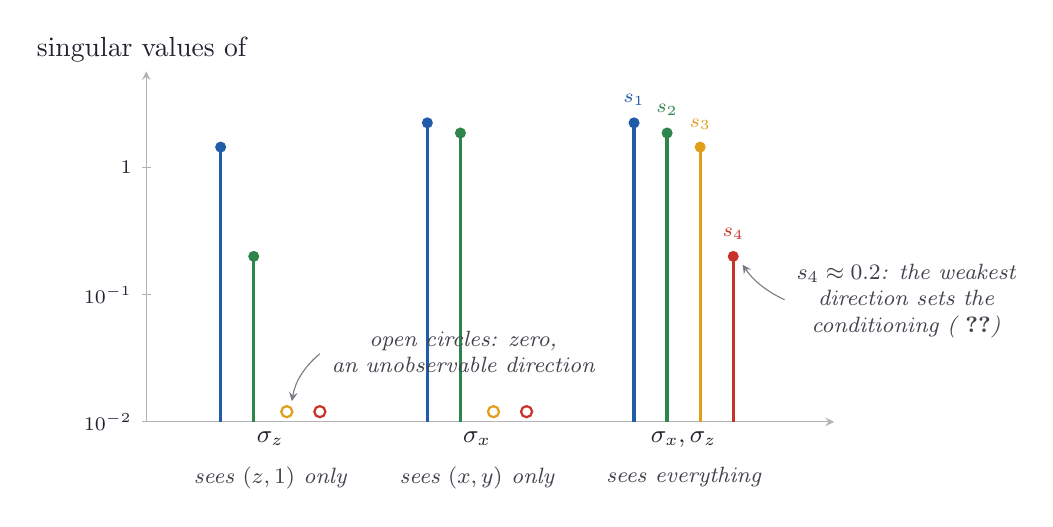
\begin{tikzpicture}[ink/.style={line width=0.9pt, ndInk}, faint/.style={line width=0.4pt, ndInk!35}, dashedink/.style={line width=0.5pt, ndInk!55, dash pattern=on 2.5pt off 2pt}, vec/.style={->, >=stealth, line width=1.2pt}, note/.style={font=\footnotesize\itshape, text=ndInk!85, align=center}, pointer/.style={->, >=stealth, line width=0.4pt, ndInk!60, shorten >=2pt, shorten <=1pt}, dot/.style={circle, fill=ndInk, inner sep=0pt, minimum size=3.4pt}, wash/.style={fill=ndSky, fill opacity=0.55}, every node/.style={text=ndInk}]
\definecolor{ndInk}{rgb}{0.13,0.13,0.18}
\definecolor{ndPaper}{rgb}{0.99,0.96,0.88}
\definecolor{ndSky}{rgb}{0.84,0.91,0.98}
\definecolor{ndRose}{rgb}{0.98,0.86,0.84}
\definecolor{ndBlue}{rgb}{0.13,0.36,0.66}
\definecolor{ndRed}{rgb}{0.78,0.20,0.16}
\definecolor{ndGold}{rgb}{0.88,0.62,0.10}
\definecolor{ndGreen}{rgb}{0.18,0.52,0.30}
\draw[faint, ->, >=stealth] (0.000,0.000) -- (8.736,0.000) node[right, text=ndInk] {};
\draw[faint, ->, >=stealth] (0.000,0.000) -- (0.000,4.452) node[above, text=ndInk] {singular values of $\Obsv$};
\draw[faint] (0.060,0.000) -- (-0.060,0.000) node[left, font=\scriptsize, text=ndInk] {$10^{-2}$};
\draw[faint] (0.060,1.615) -- (-0.060,1.615) node[left, font=\scriptsize, text=ndInk] {$10^{-1}$};
\draw[faint] (0.060,3.231) -- (-0.060,3.231) node[left, font=\scriptsize, text=ndInk] {$1$};
\draw[line width=1.2pt, ndBlue] (0.945,0.000) -- (0.945,3.489);
\fill[ndBlue] (0.945,3.489) circle (2pt);
\draw[line width=1.2pt, ndGreen] (1.365,0.000) -- (1.365,2.101);
\fill[ndGreen] (1.365,2.101) circle (2pt);
\draw[line width=0.8pt, ndGold, fill=white] (1.785,0.129) circle (2pt);
\draw[line width=0.8pt, ndRed, fill=white] (2.205,0.129) circle (2pt);
\node[below, font=\small] at (1.575,0.000) {$\sigma_z$};
\node[note, below] at (1.575,-0.450) {sees $(z,1)$ only};
\draw[line width=1.2pt, ndBlue] (3.570,0.000) -- (3.570,3.797);
\fill[ndBlue] (3.570,3.797) circle (2pt);
\draw[line width=1.2pt, ndGreen] (3.990,0.000) -- (3.990,3.668);
\fill[ndGreen] (3.990,3.668) circle (2pt);
\draw[line width=0.8pt, ndGold, fill=white] (4.410,0.129) circle (2pt);
\draw[line width=0.8pt, ndRed, fill=white] (4.830,0.129) circle (2pt);
\node[below, font=\small] at (4.200,0.000) {$\sigma_x$};
\node[note, below] at (4.200,-0.450) {sees $(x,y)$ only};
\draw[line width=1.2pt, ndBlue] (6.195,0.000) -- (6.195,3.797);
\fill[ndBlue] (6.195,3.797) circle (2pt);
\draw[line width=1.2pt, ndGreen] (6.615,0.000) -- (6.615,3.668);
\fill[ndGreen] (6.615,3.668) circle (2pt);
\draw[line width=1.2pt, ndGold] (7.035,0.000) -- (7.035,3.489);
\fill[ndGold] (7.035,3.489) circle (2pt);
\draw[line width=1.2pt, ndRed] (7.455,0.000) -- (7.455,2.101);
\fill[ndRed] (7.455,2.101) circle (2pt);
\node[below, font=\small] at (6.825,0.000) {$\sigma_x,\sigma_z$};
\node[note, below] at (6.825,-0.450) {sees everything};
\node[note, anchor=west] (z) at (2.231,0.888) {open circles: zero,\\ an unobservable direction};
\draw[pointer] (z.west) to[bend right=20] (1.838,0.194);
\node[note, anchor=west] (s) at (8.138,1.535) {$s_4\approx0.2$: the weakest\\ direction sets the\\ conditioning (\Chap~\ref{C.SampleComplexity})};
\draw[pointer] (s.west) to[bend left=15] (7.534,2.053);
\node[font=\scriptsize, text=ndBlue] at (6.195,4.087) {$s_1$};
\node[font=\scriptsize, text=ndGreen] at (6.615,3.958) {$s_2$};
\node[font=\scriptsize, text=ndGold] at (7.035,3.779) {$s_3$};
\node[font=\scriptsize, text=ndRed] at (7.455,2.392) {$s_4$};
\end{tikzpicture}
}
\caption{Singular values of the Kalman observability matrix of the embedded ($4$-dimensional) damped-qubit model for three choices of readout ($\omega=1$, $\gamma_1=0.2$, $\gamma_\phi=0.1$). Zero singular values, which belong to unobservable directions, are drawn as open circles on the lower axis. Generated by \texttt{code/ch04\_observability.py}.}\label{fig:ch04:singular}\end{figure}}
\end{frame}

\section{Identifiability}\label{sec:ch04:identifiability}

\begin{frame}\ft{Three questions}
\ona{Controllability, observability and identifiability are easily confused, since all three are decided by rank conditions. Figure~\ref{fig:ch04:threemaps} sets them side by side as properties of three maps. Controllability asks whether the map from inputs to states is onto, that is, whether every state can be reached. Observability asks whether the map from initial states to outputs is one-to-one, that is, whether different states always give different data. Identifiability asks the same question one level up, about the map from the parameters of the model to its input--output behaviour: do different parameters always give different data? The first two are questions about the states of a given model; the third is a question about the model itself, and it can fail even when the first two hold. In the language of automata, observability asks whether the states of a machine can be told apart by experiments, and identifiability whether two different machines could have produced the same table of inputs and outputs.}
\ona{\begin{figure}[H]\centering
\resizebox{\linewidth}{!}{% Generated by code/needham.py -- do not edit by hand.
\definecolor{qocA}{rgb}{0.00,0.45,0.70}
\definecolor{qocB}{rgb}{0.90,0.60,0.00}
\definecolor{qocC}{rgb}{0.00,0.62,0.45}
\definecolor{qocD}{rgb}{0.80,0.40,0.00}
\definecolor{qocE}{rgb}{0.80,0.60,0.70}
\definecolor{qocF}{rgb}{0.35,0.70,0.90}
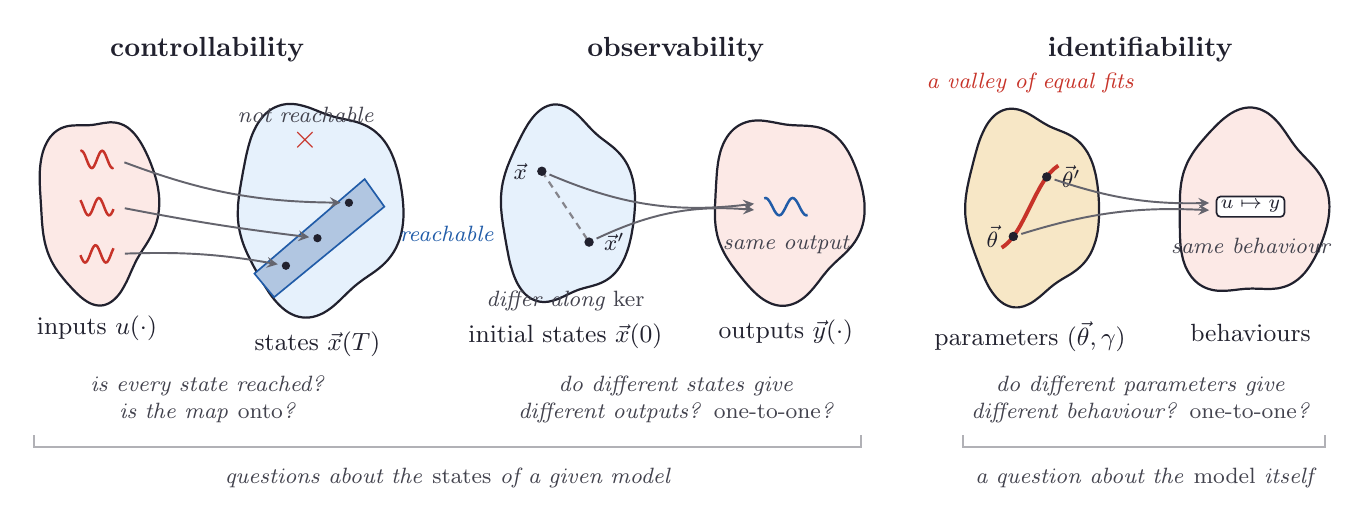
\begin{tikzpicture}[ink/.style={line width=0.9pt, ndInk}, faint/.style={line width=0.4pt, ndInk!35}, dashedink/.style={line width=0.5pt, ndInk!55, dash pattern=on 2.5pt off 2pt}, vec/.style={->, >=stealth, line width=1.2pt}, note/.style={font=\footnotesize\itshape, text=ndInk!85, align=center}, pointer/.style={->, >=stealth, line width=0.4pt, ndInk!60, shorten >=2pt, shorten <=1pt}, dot/.style={circle, fill=ndInk, inner sep=0pt, minimum size=3.4pt}, wash/.style={fill=ndSky, fill opacity=0.55}, every node/.style={text=ndInk}]
\definecolor{ndInk}{rgb}{0.13,0.13,0.18}
\definecolor{ndPaper}{rgb}{0.99,0.96,0.88}
\definecolor{ndSky}{rgb}{0.84,0.91,0.98}
\definecolor{ndRose}{rgb}{0.98,0.86,0.84}
\definecolor{ndBlue}{rgb}{0.13,0.36,0.66}
\definecolor{ndRed}{rgb}{0.78,0.20,0.16}
\definecolor{ndGold}{rgb}{0.88,0.62,0.10}
\definecolor{ndGreen}{rgb}{0.18,0.52,0.30}
\filldraw[fill=ndRose, fill opacity=0.6, draw=ndInk, line width=0.8pt] (1.690,0.000) -- (1.692,0.048) -- (1.691,0.096) -- (1.688,0.144) -- (1.682,0.191) -- (1.675,0.238) -- (1.666,0.284) -- (1.656,0.329) -- (1.644,0.373) -- (1.631,0.416) -- (1.617,0.459) -- (1.602,0.500) -- (1.587,0.541) -- (1.571,0.581) -- (1.555,0.620) -- (1.537,0.658) -- (1.520,0.696) -- (1.501,0.733) -- (1.482,0.769) -- (1.462,0.804) -- (1.441,0.838) -- (1.419,0.870) -- (1.396,0.901) -- (1.372,0.930) -- (1.347,0.956) -- (1.321,0.980) -- (1.295,1.002) -- (1.267,1.020) -- (1.238,1.036) -- (1.209,1.048) -- (1.180,1.058) -- (1.150,1.065) -- (1.120,1.069) -- (1.091,1.071) -- (1.061,1.071) -- (1.032,1.068) -- (1.004,1.065) -- (0.975,1.061) -- (0.948,1.056) -- (0.920,1.051) -- (0.893,1.046) -- (0.866,1.042) -- (0.840,1.038) -- (0.813,1.036) -- (0.786,1.034) -- (0.758,1.033) -- (0.730,1.033) -- (0.702,1.033) -- (0.672,1.033) -- (0.642,1.033) -- (0.611,1.032) -- (0.580,1.030) -- (0.548,1.026) -- (0.516,1.020) -- (0.484,1.011) -- (0.452,0.999) -- (0.420,0.983) -- (0.390,0.964) -- (0.360,0.941) -- (0.333,0.914) -- (0.306,0.884) -- (0.282,0.849) -- (0.261,0.812) -- (0.241,0.771) -- (0.224,0.728) -- (0.210,0.683) -- (0.198,0.635) -- (0.189,0.587) -- (0.182,0.538) -- (0.177,0.488) -- (0.174,0.438) -- (0.173,0.389) -- (0.173,0.340) -- (0.174,0.292) -- (0.176,0.245) -- (0.178,0.199) -- (0.181,0.154) -- (0.184,0.109) -- (0.186,0.065) -- (0.189,0.022) -- (0.192,-0.021) -- (0.194,-0.064) -- (0.197,-0.107) -- (0.199,-0.150) -- (0.202,-0.192) -- (0.206,-0.235) -- (0.210,-0.278) -- (0.215,-0.321) -- (0.221,-0.363) -- (0.229,-0.406) -- (0.237,-0.448) -- (0.247,-0.489) -- (0.259,-0.530) -- (0.271,-0.569) -- (0.286,-0.608) -- (0.301,-0.645) -- (0.318,-0.681) -- (0.336,-0.716) -- (0.355,-0.749) -- (0.375,-0.781) -- (0.396,-0.812) -- (0.417,-0.842) -- (0.439,-0.870) -- (0.462,-0.899) -- (0.484,-0.926) -- (0.507,-0.954) -- (0.531,-0.981) -- (0.555,-1.007) -- (0.579,-1.034) -- (0.604,-1.060) -- (0.629,-1.086) -- (0.655,-1.111) -- (0.682,-1.136) -- (0.709,-1.159) -- (0.738,-1.181) -- (0.767,-1.201) -- (0.797,-1.218) -- (0.828,-1.233) -- (0.860,-1.244) -- (0.892,-1.252) -- (0.924,-1.255) -- (0.957,-1.255) -- (0.989,-1.250) -- (1.021,-1.240) -- (1.052,-1.226) -- (1.082,-1.208) -- (1.111,-1.186) -- (1.139,-1.160) -- (1.166,-1.131) -- (1.191,-1.099) -- (1.214,-1.065) -- (1.236,-1.028) -- (1.256,-0.991) -- (1.276,-0.953) -- (1.294,-0.915) -- (1.311,-0.877) -- (1.327,-0.840) -- (1.343,-0.804) -- (1.359,-0.769) -- (1.375,-0.735) -- (1.391,-0.702) -- (1.407,-0.670) -- (1.425,-0.640) -- (1.442,-0.609) -- (1.461,-0.579) -- (1.480,-0.549) -- (1.500,-0.519) -- (1.520,-0.488) -- (1.540,-0.456) -- (1.560,-0.422) -- (1.580,-0.387) -- (1.599,-0.350) -- (1.616,-0.312) -- (1.633,-0.272) -- (1.648,-0.230) -- (1.661,-0.186) -- (1.672,-0.141) -- (1.680,-0.095) -- (1.686,-0.048) -- (1.690,-0.000) -- cycle;
\filldraw[fill=ndSky, fill opacity=0.6, draw=ndInk, line width=0.8pt] (4.791,0.000) -- (4.787,0.053) -- (4.782,0.106) -- (4.776,0.159) -- (4.768,0.211) -- (4.760,0.263) -- (4.750,0.314) -- (4.740,0.365) -- (4.728,0.416) -- (4.715,0.467) -- (4.700,0.517) -- (4.685,0.566) -- (4.667,0.614) -- (4.647,0.662) -- (4.626,0.708) -- (4.602,0.752) -- (4.576,0.795) -- (4.548,0.835) -- (4.518,0.873) -- (4.485,0.907) -- (4.451,0.939) -- (4.416,0.968) -- (4.378,0.994) -- (4.340,1.017) -- (4.301,1.036) -- (4.261,1.053) -- (4.221,1.068) -- (4.181,1.080) -- (4.141,1.090) -- (4.102,1.099) -- (4.063,1.107) -- (4.025,1.115) -- (3.987,1.123) -- (3.950,1.132) -- (3.913,1.141) -- (3.877,1.152) -- (3.840,1.163) -- (3.804,1.176) -- (3.767,1.190) -- (3.729,1.205) -- (3.690,1.221) -- (3.651,1.236) -- (3.610,1.252) -- (3.568,1.266) -- (3.525,1.279) -- (3.481,1.290) -- (3.436,1.299) -- (3.390,1.304) -- (3.344,1.305) -- (3.298,1.302) -- (3.252,1.294) -- (3.207,1.281) -- (3.163,1.263) -- (3.121,1.241) -- (3.081,1.213) -- (3.043,1.182) -- (3.008,1.145) -- (2.976,1.105) -- (2.946,1.062) -- (2.919,1.016) -- (2.895,0.968) -- (2.873,0.918) -- (2.854,0.867) -- (2.838,0.815) -- (2.823,0.763) -- (2.810,0.711) -- (2.798,0.660) -- (2.787,0.609) -- (2.777,0.558) -- (2.768,0.509) -- (2.758,0.459) -- (2.749,0.411) -- (2.741,0.363) -- (2.732,0.315) -- (2.724,0.267) -- (2.716,0.219) -- (2.709,0.171) -- (2.702,0.122) -- (2.697,0.074) -- (2.692,0.025) -- (2.690,-0.025) -- (2.689,-0.074) -- (2.689,-0.124) -- (2.692,-0.174) -- (2.697,-0.223) -- (2.705,-0.272) -- (2.714,-0.321) -- (2.726,-0.368) -- (2.739,-0.415) -- (2.754,-0.462) -- (2.771,-0.507) -- (2.789,-0.551) -- (2.808,-0.594) -- (2.829,-0.637) -- (2.849,-0.679) -- (2.871,-0.721) -- (2.893,-0.763) -- (2.916,-0.804) -- (2.938,-0.846) -- (2.962,-0.887) -- (2.986,-0.929) -- (3.010,-0.971) -- (3.036,-1.013) -- (3.063,-1.055) -- (3.090,-1.097) -- (3.120,-1.138) -- (3.151,-1.178) -- (3.184,-1.216) -- (3.218,-1.252) -- (3.255,-1.286) -- (3.293,-1.317) -- (3.333,-1.344) -- (3.375,-1.366) -- (3.418,-1.385) -- (3.462,-1.398) -- (3.507,-1.406) -- (3.553,-1.409) -- (3.599,-1.407) -- (3.644,-1.399) -- (3.689,-1.387) -- (3.733,-1.370) -- (3.776,-1.350) -- (3.817,-1.325) -- (3.857,-1.298) -- (3.895,-1.269) -- (3.931,-1.238) -- (3.966,-1.206) -- (4.000,-1.174) -- (4.032,-1.142) -- (4.064,-1.111) -- (4.095,-1.081) -- (4.126,-1.052) -- (4.156,-1.024) -- (4.187,-0.998) -- (4.218,-0.973) -- (4.250,-0.949) -- (4.282,-0.925) -- (4.315,-0.902) -- (4.349,-0.879) -- (4.384,-0.855) -- (4.419,-0.831) -- (4.454,-0.805) -- (4.489,-0.777) -- (4.524,-0.747) -- (4.558,-0.715) -- (4.590,-0.681) -- (4.621,-0.644) -- (4.650,-0.604) -- (4.677,-0.562) -- (4.701,-0.517) -- (4.722,-0.470) -- (4.741,-0.422) -- (4.757,-0.371) -- (4.769,-0.320) -- (4.779,-0.267) -- (4.786,-0.214) -- (4.791,-0.161) -- (4.793,-0.107) -- (4.793,-0.053) -- (4.791,-0.000) -- cycle;
\filldraw[fill=ndBlue!35, draw=ndBlue, line width=0.6pt] (2.900,-0.850) -- (4.300,0.350) -- (4.550,0.000) -- (3.150,-1.150) -- cycle;
\draw[line width=0.9pt, ndRed] (0.690,0.705) -- (0.704,0.710) -- (0.719,0.701) -- (0.733,0.681) -- (0.748,0.651) -- (0.762,0.615) -- (0.777,0.577) -- (0.791,0.542) -- (0.806,0.514) -- (0.820,0.496) -- (0.835,0.490) -- (0.849,0.497) -- (0.864,0.516) -- (0.878,0.546) -- (0.893,0.581) -- (0.907,0.619) -- (0.922,0.654) -- (0.936,0.684) -- (0.951,0.703) -- (0.965,0.710) -- (0.980,0.704) -- (0.994,0.686) -- (1.009,0.658) -- (1.023,0.623) -- (1.038,0.585) -- (1.052,0.549) -- (1.067,0.519) -- (1.081,0.499) -- (1.096,0.490) -- (1.110,0.495);
\fill[ndInk] (4.100,0.050) circle (1.5pt);
\draw[->, >=stealth, line width=0.7pt, ndInk!70, shorten <=3pt, shorten >=3pt] (1.150,0.600) to[bend left=-10] (4.100,0.050);
\draw[line width=0.9pt, ndRed] (0.690,0.083) -- (0.704,0.054) -- (0.719,0.018) -- (0.733,-0.019) -- (0.748,-0.055) -- (0.762,-0.084) -- (0.777,-0.103) -- (0.791,-0.110) -- (0.806,-0.104) -- (0.820,-0.086) -- (0.835,-0.058) -- (0.849,-0.023) -- (0.864,0.015) -- (0.878,0.051) -- (0.893,0.081) -- (0.907,0.101) -- (0.922,0.110) -- (0.936,0.105) -- (0.951,0.088) -- (0.965,0.061) -- (0.980,0.027) -- (0.994,-0.011) -- (1.009,-0.047) -- (1.023,-0.078) -- (1.038,-0.100) -- (1.052,-0.110) -- (1.067,-0.106) -- (1.081,-0.091) -- (1.096,-0.065) -- (1.110,-0.031);
\fill[ndInk] (3.700,-0.400) circle (1.5pt);
\draw[->, >=stealth, line width=0.7pt, ndInk!70, shorten <=3pt, shorten >=3pt] (1.150,0.000) to[bend left=-2] (3.700,-0.400);
\draw[line width=0.9pt, ndRed] (0.690,-0.616) -- (0.704,-0.651) -- (0.719,-0.681) -- (0.733,-0.702) -- (0.748,-0.710) -- (0.762,-0.705) -- (0.777,-0.688) -- (0.791,-0.661) -- (0.806,-0.626) -- (0.820,-0.589) -- (0.835,-0.552) -- (0.849,-0.522) -- (0.864,-0.500) -- (0.878,-0.490) -- (0.893,-0.494) -- (0.907,-0.509) -- (0.922,-0.536) -- (0.936,-0.570) -- (0.951,-0.607) -- (0.965,-0.644) -- (0.980,-0.675) -- (0.994,-0.698) -- (1.009,-0.709) -- (1.023,-0.707) -- (1.038,-0.693) -- (1.052,-0.668) -- (1.067,-0.634) -- (1.081,-0.597) -- (1.096,-0.560) -- (1.110,-0.528);
\fill[ndInk] (3.300,-0.750) circle (1.5pt);
\draw[->, >=stealth, line width=0.7pt, ndInk!70, shorten <=3pt, shorten >=3pt] (1.150,-0.600) to[bend left=6] (3.300,-0.750);
\node[font=\large, text=ndRed] at (3.550,0.850) {$\times$};
\node[note, anchor=south] at (3.550,0.950) {not reachable};
\node[note, text=ndBlue, anchor=west] at (4.620,-0.350) {reachable};
\node[font=\small] at (0.900,-1.550) {inputs $u(\cdot)$};
\node[font=\small] at (3.700,-1.750) {states $\vec x(T)$};
\node[font=\bfseries] at (2.300,2.000) {controllability};
\node[note] at (2.300,-2.450) {is every state reached?\\ is the map \emph{onto}?};
\filldraw[fill=ndSky, fill opacity=0.6, draw=ndInk, line width=0.8pt] (7.732,0.000) -- (7.733,0.049) -- (7.733,0.099) -- (7.732,0.148) -- (7.728,0.198) -- (7.723,0.247) -- (7.715,0.295) -- (7.706,0.343) -- (7.693,0.389) -- (7.679,0.435) -- (7.662,0.478) -- (7.643,0.520) -- (7.622,0.559) -- (7.599,0.596) -- (7.574,0.631) -- (7.548,0.663) -- (7.520,0.693) -- (7.492,0.721) -- (7.464,0.747) -- (7.435,0.771) -- (7.406,0.793) -- (7.378,0.815) -- (7.350,0.836) -- (7.323,0.856) -- (7.296,0.877) -- (7.270,0.898) -- (7.244,0.921) -- (7.219,0.944) -- (7.194,0.969) -- (7.169,0.994) -- (7.143,1.021) -- (7.118,1.049) -- (7.091,1.078) -- (7.064,1.107) -- (7.036,1.136) -- (7.007,1.164) -- (6.976,1.191) -- (6.944,1.216) -- (6.911,1.239) -- (6.876,1.259) -- (6.841,1.275) -- (6.805,1.287) -- (6.768,1.295) -- (6.731,1.298) -- (6.694,1.297) -- (6.658,1.290) -- (6.622,1.279) -- (6.586,1.263) -- (6.552,1.243) -- (6.520,1.219) -- (6.488,1.191) -- (6.458,1.160) -- (6.430,1.127) -- (6.404,1.092) -- (6.378,1.055) -- (6.355,1.017) -- (6.332,0.978) -- (6.311,0.939) -- (6.290,0.899) -- (6.270,0.860) -- (6.251,0.821) -- (6.233,0.782) -- (6.214,0.743) -- (6.196,0.704) -- (6.179,0.666) -- (6.162,0.627) -- (6.145,0.588) -- (6.129,0.548) -- (6.113,0.508) -- (6.099,0.467) -- (6.085,0.426) -- (6.073,0.383) -- (6.062,0.340) -- (6.052,0.296) -- (6.044,0.251) -- (6.038,0.206) -- (6.034,0.160) -- (6.031,0.115) -- (6.030,0.069) -- (6.031,0.023) -- (6.033,-0.023) -- (6.037,-0.068) -- (6.041,-0.113) -- (6.047,-0.158) -- (6.053,-0.202) -- (6.059,-0.246) -- (6.067,-0.291) -- (6.074,-0.335) -- (6.081,-0.379) -- (6.089,-0.423) -- (6.097,-0.468) -- (6.105,-0.514) -- (6.114,-0.560) -- (6.123,-0.607) -- (6.132,-0.654) -- (6.143,-0.701) -- (6.155,-0.749) -- (6.169,-0.796) -- (6.184,-0.844) -- (6.201,-0.890) -- (6.220,-0.934) -- (6.241,-0.977) -- (6.265,-1.018) -- (6.291,-1.055) -- (6.319,-1.090) -- (6.349,-1.120) -- (6.381,-1.146) -- (6.415,-1.168) -- (6.450,-1.185) -- (6.486,-1.198) -- (6.523,-1.206) -- (6.560,-1.210) -- (6.598,-1.210) -- (6.635,-1.206) -- (6.671,-1.198) -- (6.707,-1.188) -- (6.742,-1.176) -- (6.777,-1.163) -- (6.810,-1.148) -- (6.842,-1.133) -- (6.873,-1.117) -- (6.904,-1.103) -- (6.934,-1.089) -- (6.964,-1.076) -- (6.993,-1.064) -- (7.022,-1.053) -- (7.052,-1.044) -- (7.082,-1.035) -- (7.112,-1.027) -- (7.143,-1.019) -- (7.174,-1.011) -- (7.205,-1.002) -- (7.237,-0.992) -- (7.270,-0.981) -- (7.302,-0.968) -- (7.334,-0.953) -- (7.366,-0.935) -- (7.397,-0.915) -- (7.428,-0.891) -- (7.457,-0.865) -- (7.485,-0.836) -- (7.511,-0.804) -- (7.536,-0.770) -- (7.559,-0.733) -- (7.580,-0.694) -- (7.600,-0.654) -- (7.617,-0.611) -- (7.633,-0.568) -- (7.648,-0.523) -- (7.661,-0.477) -- (7.672,-0.431) -- (7.683,-0.385) -- (7.692,-0.338) -- (7.700,-0.290) -- (7.708,-0.242) -- (7.715,-0.195) -- (7.720,-0.146) -- (7.725,-0.098) -- (7.729,-0.049) -- (7.732,-0.000) -- cycle;
\filldraw[fill=ndRose, fill opacity=0.6, draw=ndInk, line width=0.8pt] (10.649,0.000) -- (10.647,0.048) -- (10.642,0.095) -- (10.635,0.142) -- (10.627,0.189) -- (10.617,0.234) -- (10.606,0.280) -- (10.594,0.324) -- (10.580,0.368) -- (10.566,0.412) -- (10.551,0.455) -- (10.535,0.497) -- (10.518,0.539) -- (10.500,0.581) -- (10.481,0.622) -- (10.461,0.661) -- (10.440,0.700) -- (10.416,0.738) -- (10.392,0.774) -- (10.366,0.808) -- (10.338,0.841) -- (10.308,0.871) -- (10.277,0.899) -- (10.244,0.924) -- (10.211,0.946) -- (10.176,0.965) -- (10.140,0.981) -- (10.103,0.995) -- (10.066,1.006) -- (10.029,1.014) -- (9.992,1.020) -- (9.955,1.024) -- (9.918,1.027) -- (9.882,1.029) -- (9.847,1.030) -- (9.812,1.031) -- (9.777,1.033) -- (9.743,1.034) -- (9.709,1.037) -- (9.675,1.040) -- (9.641,1.044) -- (9.607,1.050) -- (9.572,1.056) -- (9.537,1.063) -- (9.500,1.070) -- (9.463,1.077) -- (9.424,1.083) -- (9.385,1.089) -- (9.345,1.093) -- (9.304,1.095) -- (9.263,1.094) -- (9.221,1.090) -- (9.180,1.083) -- (9.139,1.071) -- (9.099,1.056) -- (9.061,1.037) -- (9.024,1.014) -- (8.989,0.986) -- (8.957,0.955) -- (8.927,0.920) -- (8.900,0.882) -- (8.876,0.841) -- (8.854,0.797) -- (8.836,0.752) -- (8.820,0.706) -- (8.808,0.658) -- (8.797,0.610) -- (8.788,0.562) -- (8.782,0.514) -- (8.776,0.466) -- (8.772,0.419) -- (8.769,0.373) -- (8.766,0.327) -- (8.763,0.282) -- (8.761,0.238) -- (8.758,0.194) -- (8.756,0.151) -- (8.754,0.108) -- (8.752,0.065) -- (8.750,0.022) -- (8.749,-0.022) -- (8.748,-0.065) -- (8.748,-0.108) -- (8.749,-0.152) -- (8.752,-0.195) -- (8.756,-0.239) -- (8.762,-0.282) -- (8.770,-0.325) -- (8.779,-0.368) -- (8.791,-0.410) -- (8.804,-0.451) -- (8.820,-0.491) -- (8.837,-0.530) -- (8.855,-0.568) -- (8.875,-0.605) -- (8.896,-0.641) -- (8.918,-0.676) -- (8.941,-0.711) -- (8.964,-0.744) -- (8.989,-0.777) -- (9.013,-0.810) -- (9.038,-0.842) -- (9.064,-0.875) -- (9.090,-0.907) -- (9.116,-0.939) -- (9.143,-0.971) -- (9.171,-1.003) -- (9.200,-1.035) -- (9.230,-1.066) -- (9.262,-1.097) -- (9.294,-1.126) -- (9.328,-1.153) -- (9.363,-1.178) -- (9.400,-1.200) -- (9.438,-1.220) -- (9.477,-1.236) -- (9.517,-1.248) -- (9.558,-1.256) -- (9.599,-1.259) -- (9.640,-1.258) -- (9.681,-1.252) -- (9.721,-1.242) -- (9.761,-1.227) -- (9.799,-1.209) -- (9.836,-1.186) -- (9.872,-1.161) -- (9.906,-1.132) -- (9.938,-1.102) -- (9.968,-1.070) -- (9.997,-1.037) -- (10.025,-1.003) -- (10.051,-0.970) -- (10.077,-0.937) -- (10.101,-0.904) -- (10.125,-0.873) -- (10.150,-0.843) -- (10.174,-0.814) -- (10.198,-0.786) -- (10.224,-0.759) -- (10.250,-0.733) -- (10.276,-0.708) -- (10.304,-0.682) -- (10.332,-0.656) -- (10.361,-0.630) -- (10.390,-0.603) -- (10.419,-0.575) -- (10.447,-0.544) -- (10.475,-0.513) -- (10.502,-0.479) -- (10.528,-0.443) -- (10.551,-0.405) -- (10.573,-0.365) -- (10.592,-0.324) -- (10.609,-0.280) -- (10.623,-0.236) -- (10.634,-0.190) -- (10.642,-0.143) -- (10.647,-0.096) -- (10.649,-0.048) -- (10.649,-0.000) -- cycle;
\draw[dashedink, line width=0.8pt] (6.550,0.450) -- (7.150,-0.450);
\node[dot, label={[font=\footnotesize]left:$\vec x$}] at (6.550,0.450) {};
\node[dot, label={[font=\footnotesize]right:$\vec x'$}] at (7.150,-0.450) {};
\draw[line width=0.9pt, ndBlue] (9.375,0.105) -- (9.394,0.110) -- (9.413,0.101) -- (9.432,0.081) -- (9.451,0.051) -- (9.470,0.015) -- (9.489,-0.023) -- (9.508,-0.058) -- (9.527,-0.086) -- (9.546,-0.104) -- (9.565,-0.110) -- (9.584,-0.103) -- (9.603,-0.084) -- (9.622,-0.054) -- (9.641,-0.019) -- (9.659,0.019) -- (9.678,0.054) -- (9.697,0.084) -- (9.716,0.103) -- (9.735,0.110) -- (9.754,0.104) -- (9.773,0.086) -- (9.792,0.058) -- (9.811,0.023) -- (9.830,-0.015) -- (9.849,-0.051) -- (9.868,-0.081) -- (9.887,-0.101) -- (9.906,-0.110) -- (9.925,-0.105);
\draw[->, >=stealth, line width=0.7pt, ndInk!70, shorten <=3pt, shorten >=3pt] (6.550,0.450) to[bend left=-15] (9.350,0.050);
\draw[->, >=stealth, line width=0.7pt, ndInk!70, shorten <=3pt, shorten >=3pt] (7.150,-0.450) to[bend left=15] (9.350,-0.050);
\node[note, anchor=north] at (9.650,-0.250) {same output};
\node[note, anchor=north] at (6.850,-0.950) {differ along $\ker\OM$};
\node[font=\small] at (6.850,-1.650) {initial states $\vec x(0)$};
\node[font=\small] at (9.650,-1.600) {outputs $\vec y(\cdot)$};
\node[font=\bfseries] at (8.250,2.000) {observability};
\node[note] at (8.250,-2.450) {do different states give\\ different outputs? \emph{one-to-one}?};
\filldraw[fill=ndGold!25, draw=ndInk, line width=0.8pt] (13.627,0.000) -- (13.625,0.049) -- (13.623,0.098) -- (13.619,0.146) -- (13.615,0.195) -- (13.610,0.243) -- (13.604,0.291) -- (13.596,0.339) -- (13.588,0.387) -- (13.577,0.434) -- (13.565,0.480) -- (13.552,0.526) -- (13.536,0.570) -- (13.519,0.612) -- (13.499,0.653) -- (13.478,0.692) -- (13.454,0.728) -- (13.429,0.762) -- (13.402,0.794) -- (13.374,0.822) -- (13.345,0.848) -- (13.314,0.871) -- (13.284,0.892) -- (13.252,0.910) -- (13.221,0.926) -- (13.189,0.941) -- (13.158,0.954) -- (13.127,0.966) -- (13.097,0.978) -- (13.067,0.990) -- (13.038,1.002) -- (13.009,1.015) -- (12.981,1.029) -- (12.952,1.045) -- (12.924,1.061) -- (12.895,1.078) -- (12.866,1.097) -- (12.836,1.116) -- (12.806,1.136) -- (12.774,1.155) -- (12.742,1.174) -- (12.708,1.192) -- (12.674,1.208) -- (12.638,1.222) -- (12.602,1.233) -- (12.565,1.240) -- (12.528,1.244) -- (12.491,1.243) -- (12.454,1.238) -- (12.417,1.228) -- (12.381,1.213) -- (12.347,1.194) -- (12.314,1.171) -- (12.283,1.143) -- (12.253,1.111) -- (12.226,1.076) -- (12.200,1.037) -- (12.177,0.997) -- (12.156,0.954) -- (12.136,0.910) -- (12.118,0.866) -- (12.102,0.820) -- (12.087,0.775) -- (12.074,0.729) -- (12.061,0.684) -- (12.049,0.639) -- (12.037,0.595) -- (12.026,0.551) -- (12.015,0.507) -- (12.004,0.464) -- (11.993,0.421) -- (11.983,0.378) -- (11.973,0.335) -- (11.964,0.292) -- (11.955,0.248) -- (11.947,0.204) -- (11.940,0.159) -- (11.934,0.114) -- (11.930,0.069) -- (11.927,0.023) -- (11.926,-0.023) -- (11.927,-0.069) -- (11.929,-0.115) -- (11.934,-0.160) -- (11.940,-0.206) -- (11.947,-0.250) -- (11.956,-0.294) -- (11.966,-0.338) -- (11.978,-0.381) -- (11.990,-0.423) -- (12.003,-0.464) -- (12.017,-0.506) -- (12.031,-0.547) -- (12.045,-0.587) -- (12.060,-0.628) -- (12.075,-0.669) -- (12.091,-0.711) -- (12.106,-0.752) -- (12.123,-0.794) -- (12.140,-0.836) -- (12.158,-0.879) -- (12.177,-0.921) -- (12.197,-0.963) -- (12.218,-1.004) -- (12.241,-1.044) -- (12.266,-1.082) -- (12.293,-1.118) -- (12.321,-1.152) -- (12.351,-1.183) -- (12.383,-1.210) -- (12.416,-1.233) -- (12.450,-1.251) -- (12.486,-1.265) -- (12.522,-1.275) -- (12.559,-1.279) -- (12.596,-1.279) -- (12.633,-1.274) -- (12.670,-1.265) -- (12.706,-1.251) -- (12.741,-1.235) -- (12.776,-1.216) -- (12.809,-1.194) -- (12.840,-1.170) -- (12.871,-1.146) -- (12.901,-1.121) -- (12.929,-1.096) -- (12.957,-1.071) -- (12.985,-1.047) -- (13.011,-1.024) -- (13.038,-1.003) -- (13.065,-0.982) -- (13.092,-0.963) -- (13.119,-0.945) -- (13.147,-0.927) -- (13.175,-0.910) -- (13.204,-0.893) -- (13.233,-0.876) -- (13.263,-0.858) -- (13.293,-0.838) -- (13.323,-0.817) -- (13.353,-0.794) -- (13.382,-0.769) -- (13.411,-0.742) -- (13.438,-0.712) -- (13.465,-0.680) -- (13.489,-0.644) -- (13.512,-0.607) -- (13.533,-0.567) -- (13.551,-0.525) -- (13.567,-0.481) -- (13.582,-0.436) -- (13.594,-0.390) -- (13.604,-0.342) -- (13.612,-0.294) -- (13.618,-0.245) -- (13.622,-0.196) -- (13.625,-0.147) -- (13.627,-0.098) -- (13.627,-0.049) -- (13.627,-0.000) -- cycle;
\filldraw[fill=ndRose, fill opacity=0.6, draw=ndInk, line width=0.8pt] (16.552,0.000) -- (16.551,0.048) -- (16.546,0.096) -- (16.539,0.143) -- (16.529,0.189) -- (16.515,0.234) -- (16.499,0.278) -- (16.481,0.320) -- (16.460,0.360) -- (16.437,0.399) -- (16.412,0.435) -- (16.386,0.470) -- (16.359,0.503) -- (16.331,0.534) -- (16.304,0.564) -- (16.276,0.592) -- (16.249,0.620) -- (16.222,0.647) -- (16.197,0.675) -- (16.172,0.702) -- (16.147,0.730) -- (16.124,0.759) -- (16.101,0.790) -- (16.078,0.821) -- (16.056,0.853) -- (16.033,0.887) -- (16.010,0.921) -- (15.986,0.956) -- (15.960,0.992) -- (15.934,1.027) -- (15.906,1.062) -- (15.876,1.095) -- (15.844,1.127) -- (15.811,1.156) -- (15.776,1.183) -- (15.739,1.206) -- (15.701,1.225) -- (15.662,1.241) -- (15.622,1.251) -- (15.581,1.258) -- (15.540,1.260) -- (15.499,1.257) -- (15.458,1.250) -- (15.418,1.239) -- (15.379,1.224) -- (15.340,1.206) -- (15.303,1.185) -- (15.267,1.161) -- (15.233,1.136) -- (15.199,1.109) -- (15.167,1.081) -- (15.136,1.052) -- (15.106,1.022) -- (15.077,0.992) -- (15.048,0.962) -- (15.020,0.932) -- (14.993,0.902) -- (14.966,0.871) -- (14.940,0.841) -- (14.913,0.810) -- (14.888,0.778) -- (14.863,0.746) -- (14.839,0.713) -- (14.816,0.679) -- (14.794,0.643) -- (14.773,0.607) -- (14.753,0.570) -- (14.736,0.531) -- (14.720,0.491) -- (14.705,0.450) -- (14.693,0.409) -- (14.683,0.367) -- (14.674,0.324) -- (14.667,0.281) -- (14.662,0.237) -- (14.658,0.194) -- (14.655,0.151) -- (14.654,0.108) -- (14.653,0.064) -- (14.652,0.021) -- (14.652,-0.021) -- (14.652,-0.065) -- (14.652,-0.108) -- (14.652,-0.151) -- (14.652,-0.195) -- (14.652,-0.240) -- (14.653,-0.285) -- (14.653,-0.331) -- (14.655,-0.378) -- (14.657,-0.426) -- (14.660,-0.474) -- (14.665,-0.523) -- (14.672,-0.572) -- (14.682,-0.621) -- (14.693,-0.669) -- (14.708,-0.716) -- (14.725,-0.762) -- (14.746,-0.806) -- (14.770,-0.847) -- (14.796,-0.886) -- (14.826,-0.921) -- (14.858,-0.953) -- (14.892,-0.981) -- (14.929,-1.005) -- (14.967,-1.025) -- (15.007,-1.041) -- (15.048,-1.053) -- (15.089,-1.062) -- (15.130,-1.067) -- (15.171,-1.069) -- (15.212,-1.069) -- (15.252,-1.067) -- (15.291,-1.064) -- (15.329,-1.060) -- (15.366,-1.056) -- (15.403,-1.051) -- (15.438,-1.048) -- (15.473,-1.044) -- (15.507,-1.042) -- (15.542,-1.041) -- (15.575,-1.040) -- (15.610,-1.041) -- (15.644,-1.042) -- (15.679,-1.043) -- (15.714,-1.044) -- (15.750,-1.045) -- (15.786,-1.045) -- (15.823,-1.044) -- (15.860,-1.041) -- (15.897,-1.037) -- (15.935,-1.029) -- (15.972,-1.020) -- (16.009,-1.007) -- (16.045,-0.992) -- (16.080,-0.973) -- (16.114,-0.952) -- (16.147,-0.928) -- (16.179,-0.901) -- (16.209,-0.872) -- (16.238,-0.841) -- (16.265,-0.807) -- (16.290,-0.772) -- (16.314,-0.736) -- (16.337,-0.698) -- (16.359,-0.660) -- (16.379,-0.620) -- (16.399,-0.580) -- (16.418,-0.539) -- (16.435,-0.498) -- (16.452,-0.456) -- (16.469,-0.413) -- (16.484,-0.370) -- (16.498,-0.326) -- (16.511,-0.281) -- (16.523,-0.236) -- (16.533,-0.190) -- (16.541,-0.143) -- (16.547,-0.096) -- (16.551,-0.048) -- (16.552,-0.000) -- cycle;
\draw[line width=1.4pt, ndRed] (12.390,-0.521) -- (12.408,-0.509) -- (12.427,-0.495) -- (12.445,-0.480) -- (12.464,-0.463) -- (12.482,-0.444) -- (12.501,-0.424) -- (12.519,-0.402) -- (12.538,-0.378) -- (12.556,-0.352) -- (12.575,-0.325) -- (12.593,-0.296) -- (12.612,-0.265) -- (12.630,-0.233) -- (12.648,-0.199) -- (12.667,-0.165) -- (12.685,-0.129) -- (12.704,-0.093) -- (12.722,-0.056) -- (12.741,-0.019) -- (12.759,0.019) -- (12.778,0.056) -- (12.796,0.093) -- (12.815,0.129) -- (12.833,0.165) -- (12.852,0.199) -- (12.870,0.233) -- (12.888,0.265) -- (12.907,0.296) -- (12.925,0.325) -- (12.944,0.352) -- (12.962,0.378) -- (12.981,0.402) -- (12.999,0.424) -- (13.018,0.444) -- (13.036,0.463) -- (13.055,0.480) -- (13.073,0.495) -- (13.092,0.509) -- (13.110,0.521);
\node[dot, label={[font=\footnotesize]left:$\vec\theta$}] at (12.538,-0.378) {};
\node[dot, label={[font=\footnotesize]right:$\vec\theta'$}] at (12.962,0.378) {};
\node[draw=ndInk, line width=0.6pt, rounded corners=1.5pt, fill=white, font=\scriptsize, inner sep=1.5pt] at (15.550,0.000) {$u\mapsto y$};
\draw[->, >=stealth, line width=0.7pt, ndInk!70, shorten <=3pt, shorten >=3pt] (12.538,-0.378) to[bend left=10] (15.130,-0.050);
\draw[->, >=stealth, line width=0.7pt, ndInk!70, shorten <=3pt, shorten >=3pt] (12.962,0.378) to[bend left=-10] (15.130,0.050);
\node[note, anchor=north] at (15.550,-0.280) {same behaviour};
\node[note, text=ndRed, anchor=south] at (12.750,1.320) {a valley of equal fits};
\node[font=\small] at (12.750,-1.650) {parameters $(\vec\theta,\gamma)$};
\node[font=\small] at (15.550,-1.600) {behaviours};
\node[font=\bfseries] at (14.150,2.000) {identifiability};
\node[note] at (14.150,-2.450) {do different parameters give\\ different behaviour? \emph{one-to-one}?};
\draw[faint, line width=0.7pt] (0.1,-2.9) -- (0.1,-3.05) -- (10.6,-3.05) -- (10.6,-2.9);
\node[note] at (5.35,-3.45) {questions about the \emph{states} of a given model};
\draw[faint, line width=0.7pt] (11.9,-2.9) -- (11.9,-3.05) -- (16.5,-3.05) -- (16.5,-2.9);
\node[note] at (14.2,-3.45) {a question about the \emph{model} itself};
\end{tikzpicture}
}
\caption{Three questions, three maps. Controllability: is the map from inputs to states onto? The reachable states form the blue band, and a state outside it is marked. Observability: is the map from initial states to outputs one-to-one? Two states that differ along $\ker\OM$ give the same output. Identifiability: is the map from parameters to input--output behaviour one-to-one? All parameters on the red curve give the same behaviour. Generated by \texttt{code/ch04\_threemaps.py}.}\label{fig:ch04:threemaps}
\end{figure}}
\onp{\begin{center}\resizebox{\linewidth}{!}{% Generated by code/needham.py -- do not edit by hand.
\definecolor{qocA}{rgb}{0.00,0.45,0.70}
\definecolor{qocB}{rgb}{0.90,0.60,0.00}
\definecolor{qocC}{rgb}{0.00,0.62,0.45}
\definecolor{qocD}{rgb}{0.80,0.40,0.00}
\definecolor{qocE}{rgb}{0.80,0.60,0.70}
\definecolor{qocF}{rgb}{0.35,0.70,0.90}
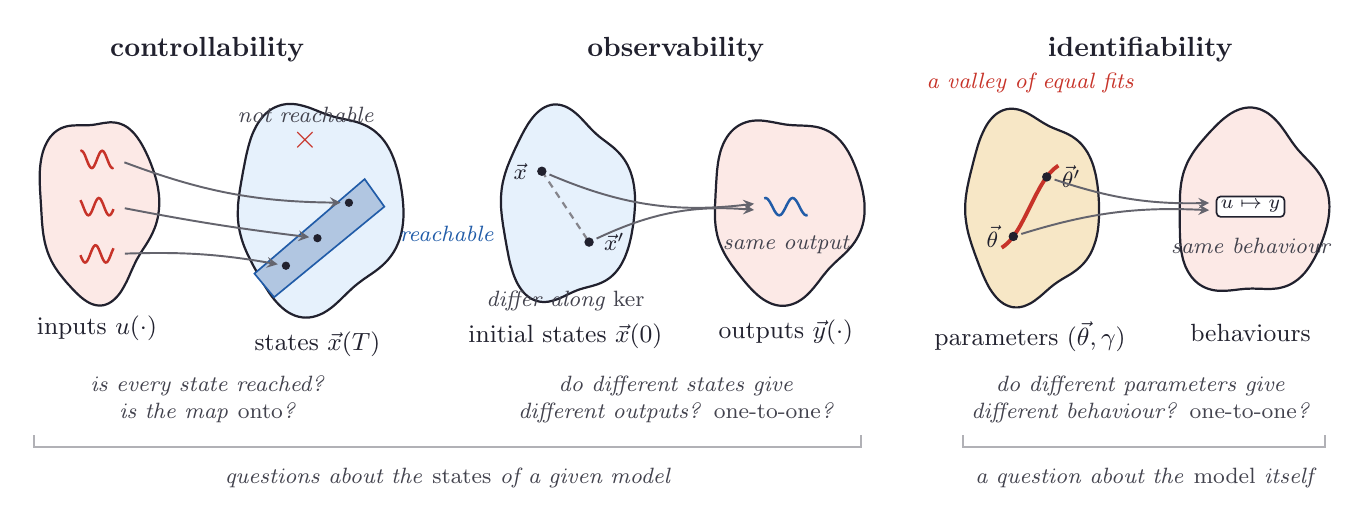
\begin{tikzpicture}[ink/.style={line width=0.9pt, ndInk}, faint/.style={line width=0.4pt, ndInk!35}, dashedink/.style={line width=0.5pt, ndInk!55, dash pattern=on 2.5pt off 2pt}, vec/.style={->, >=stealth, line width=1.2pt}, note/.style={font=\footnotesize\itshape, text=ndInk!85, align=center}, pointer/.style={->, >=stealth, line width=0.4pt, ndInk!60, shorten >=2pt, shorten <=1pt}, dot/.style={circle, fill=ndInk, inner sep=0pt, minimum size=3.4pt}, wash/.style={fill=ndSky, fill opacity=0.55}, every node/.style={text=ndInk}]
\definecolor{ndInk}{rgb}{0.13,0.13,0.18}
\definecolor{ndPaper}{rgb}{0.99,0.96,0.88}
\definecolor{ndSky}{rgb}{0.84,0.91,0.98}
\definecolor{ndRose}{rgb}{0.98,0.86,0.84}
\definecolor{ndBlue}{rgb}{0.13,0.36,0.66}
\definecolor{ndRed}{rgb}{0.78,0.20,0.16}
\definecolor{ndGold}{rgb}{0.88,0.62,0.10}
\definecolor{ndGreen}{rgb}{0.18,0.52,0.30}
\filldraw[fill=ndRose, fill opacity=0.6, draw=ndInk, line width=0.8pt] (1.690,0.000) -- (1.692,0.048) -- (1.691,0.096) -- (1.688,0.144) -- (1.682,0.191) -- (1.675,0.238) -- (1.666,0.284) -- (1.656,0.329) -- (1.644,0.373) -- (1.631,0.416) -- (1.617,0.459) -- (1.602,0.500) -- (1.587,0.541) -- (1.571,0.581) -- (1.555,0.620) -- (1.537,0.658) -- (1.520,0.696) -- (1.501,0.733) -- (1.482,0.769) -- (1.462,0.804) -- (1.441,0.838) -- (1.419,0.870) -- (1.396,0.901) -- (1.372,0.930) -- (1.347,0.956) -- (1.321,0.980) -- (1.295,1.002) -- (1.267,1.020) -- (1.238,1.036) -- (1.209,1.048) -- (1.180,1.058) -- (1.150,1.065) -- (1.120,1.069) -- (1.091,1.071) -- (1.061,1.071) -- (1.032,1.068) -- (1.004,1.065) -- (0.975,1.061) -- (0.948,1.056) -- (0.920,1.051) -- (0.893,1.046) -- (0.866,1.042) -- (0.840,1.038) -- (0.813,1.036) -- (0.786,1.034) -- (0.758,1.033) -- (0.730,1.033) -- (0.702,1.033) -- (0.672,1.033) -- (0.642,1.033) -- (0.611,1.032) -- (0.580,1.030) -- (0.548,1.026) -- (0.516,1.020) -- (0.484,1.011) -- (0.452,0.999) -- (0.420,0.983) -- (0.390,0.964) -- (0.360,0.941) -- (0.333,0.914) -- (0.306,0.884) -- (0.282,0.849) -- (0.261,0.812) -- (0.241,0.771) -- (0.224,0.728) -- (0.210,0.683) -- (0.198,0.635) -- (0.189,0.587) -- (0.182,0.538) -- (0.177,0.488) -- (0.174,0.438) -- (0.173,0.389) -- (0.173,0.340) -- (0.174,0.292) -- (0.176,0.245) -- (0.178,0.199) -- (0.181,0.154) -- (0.184,0.109) -- (0.186,0.065) -- (0.189,0.022) -- (0.192,-0.021) -- (0.194,-0.064) -- (0.197,-0.107) -- (0.199,-0.150) -- (0.202,-0.192) -- (0.206,-0.235) -- (0.210,-0.278) -- (0.215,-0.321) -- (0.221,-0.363) -- (0.229,-0.406) -- (0.237,-0.448) -- (0.247,-0.489) -- (0.259,-0.530) -- (0.271,-0.569) -- (0.286,-0.608) -- (0.301,-0.645) -- (0.318,-0.681) -- (0.336,-0.716) -- (0.355,-0.749) -- (0.375,-0.781) -- (0.396,-0.812) -- (0.417,-0.842) -- (0.439,-0.870) -- (0.462,-0.899) -- (0.484,-0.926) -- (0.507,-0.954) -- (0.531,-0.981) -- (0.555,-1.007) -- (0.579,-1.034) -- (0.604,-1.060) -- (0.629,-1.086) -- (0.655,-1.111) -- (0.682,-1.136) -- (0.709,-1.159) -- (0.738,-1.181) -- (0.767,-1.201) -- (0.797,-1.218) -- (0.828,-1.233) -- (0.860,-1.244) -- (0.892,-1.252) -- (0.924,-1.255) -- (0.957,-1.255) -- (0.989,-1.250) -- (1.021,-1.240) -- (1.052,-1.226) -- (1.082,-1.208) -- (1.111,-1.186) -- (1.139,-1.160) -- (1.166,-1.131) -- (1.191,-1.099) -- (1.214,-1.065) -- (1.236,-1.028) -- (1.256,-0.991) -- (1.276,-0.953) -- (1.294,-0.915) -- (1.311,-0.877) -- (1.327,-0.840) -- (1.343,-0.804) -- (1.359,-0.769) -- (1.375,-0.735) -- (1.391,-0.702) -- (1.407,-0.670) -- (1.425,-0.640) -- (1.442,-0.609) -- (1.461,-0.579) -- (1.480,-0.549) -- (1.500,-0.519) -- (1.520,-0.488) -- (1.540,-0.456) -- (1.560,-0.422) -- (1.580,-0.387) -- (1.599,-0.350) -- (1.616,-0.312) -- (1.633,-0.272) -- (1.648,-0.230) -- (1.661,-0.186) -- (1.672,-0.141) -- (1.680,-0.095) -- (1.686,-0.048) -- (1.690,-0.000) -- cycle;
\filldraw[fill=ndSky, fill opacity=0.6, draw=ndInk, line width=0.8pt] (4.791,0.000) -- (4.787,0.053) -- (4.782,0.106) -- (4.776,0.159) -- (4.768,0.211) -- (4.760,0.263) -- (4.750,0.314) -- (4.740,0.365) -- (4.728,0.416) -- (4.715,0.467) -- (4.700,0.517) -- (4.685,0.566) -- (4.667,0.614) -- (4.647,0.662) -- (4.626,0.708) -- (4.602,0.752) -- (4.576,0.795) -- (4.548,0.835) -- (4.518,0.873) -- (4.485,0.907) -- (4.451,0.939) -- (4.416,0.968) -- (4.378,0.994) -- (4.340,1.017) -- (4.301,1.036) -- (4.261,1.053) -- (4.221,1.068) -- (4.181,1.080) -- (4.141,1.090) -- (4.102,1.099) -- (4.063,1.107) -- (4.025,1.115) -- (3.987,1.123) -- (3.950,1.132) -- (3.913,1.141) -- (3.877,1.152) -- (3.840,1.163) -- (3.804,1.176) -- (3.767,1.190) -- (3.729,1.205) -- (3.690,1.221) -- (3.651,1.236) -- (3.610,1.252) -- (3.568,1.266) -- (3.525,1.279) -- (3.481,1.290) -- (3.436,1.299) -- (3.390,1.304) -- (3.344,1.305) -- (3.298,1.302) -- (3.252,1.294) -- (3.207,1.281) -- (3.163,1.263) -- (3.121,1.241) -- (3.081,1.213) -- (3.043,1.182) -- (3.008,1.145) -- (2.976,1.105) -- (2.946,1.062) -- (2.919,1.016) -- (2.895,0.968) -- (2.873,0.918) -- (2.854,0.867) -- (2.838,0.815) -- (2.823,0.763) -- (2.810,0.711) -- (2.798,0.660) -- (2.787,0.609) -- (2.777,0.558) -- (2.768,0.509) -- (2.758,0.459) -- (2.749,0.411) -- (2.741,0.363) -- (2.732,0.315) -- (2.724,0.267) -- (2.716,0.219) -- (2.709,0.171) -- (2.702,0.122) -- (2.697,0.074) -- (2.692,0.025) -- (2.690,-0.025) -- (2.689,-0.074) -- (2.689,-0.124) -- (2.692,-0.174) -- (2.697,-0.223) -- (2.705,-0.272) -- (2.714,-0.321) -- (2.726,-0.368) -- (2.739,-0.415) -- (2.754,-0.462) -- (2.771,-0.507) -- (2.789,-0.551) -- (2.808,-0.594) -- (2.829,-0.637) -- (2.849,-0.679) -- (2.871,-0.721) -- (2.893,-0.763) -- (2.916,-0.804) -- (2.938,-0.846) -- (2.962,-0.887) -- (2.986,-0.929) -- (3.010,-0.971) -- (3.036,-1.013) -- (3.063,-1.055) -- (3.090,-1.097) -- (3.120,-1.138) -- (3.151,-1.178) -- (3.184,-1.216) -- (3.218,-1.252) -- (3.255,-1.286) -- (3.293,-1.317) -- (3.333,-1.344) -- (3.375,-1.366) -- (3.418,-1.385) -- (3.462,-1.398) -- (3.507,-1.406) -- (3.553,-1.409) -- (3.599,-1.407) -- (3.644,-1.399) -- (3.689,-1.387) -- (3.733,-1.370) -- (3.776,-1.350) -- (3.817,-1.325) -- (3.857,-1.298) -- (3.895,-1.269) -- (3.931,-1.238) -- (3.966,-1.206) -- (4.000,-1.174) -- (4.032,-1.142) -- (4.064,-1.111) -- (4.095,-1.081) -- (4.126,-1.052) -- (4.156,-1.024) -- (4.187,-0.998) -- (4.218,-0.973) -- (4.250,-0.949) -- (4.282,-0.925) -- (4.315,-0.902) -- (4.349,-0.879) -- (4.384,-0.855) -- (4.419,-0.831) -- (4.454,-0.805) -- (4.489,-0.777) -- (4.524,-0.747) -- (4.558,-0.715) -- (4.590,-0.681) -- (4.621,-0.644) -- (4.650,-0.604) -- (4.677,-0.562) -- (4.701,-0.517) -- (4.722,-0.470) -- (4.741,-0.422) -- (4.757,-0.371) -- (4.769,-0.320) -- (4.779,-0.267) -- (4.786,-0.214) -- (4.791,-0.161) -- (4.793,-0.107) -- (4.793,-0.053) -- (4.791,-0.000) -- cycle;
\filldraw[fill=ndBlue!35, draw=ndBlue, line width=0.6pt] (2.900,-0.850) -- (4.300,0.350) -- (4.550,0.000) -- (3.150,-1.150) -- cycle;
\draw[line width=0.9pt, ndRed] (0.690,0.705) -- (0.704,0.710) -- (0.719,0.701) -- (0.733,0.681) -- (0.748,0.651) -- (0.762,0.615) -- (0.777,0.577) -- (0.791,0.542) -- (0.806,0.514) -- (0.820,0.496) -- (0.835,0.490) -- (0.849,0.497) -- (0.864,0.516) -- (0.878,0.546) -- (0.893,0.581) -- (0.907,0.619) -- (0.922,0.654) -- (0.936,0.684) -- (0.951,0.703) -- (0.965,0.710) -- (0.980,0.704) -- (0.994,0.686) -- (1.009,0.658) -- (1.023,0.623) -- (1.038,0.585) -- (1.052,0.549) -- (1.067,0.519) -- (1.081,0.499) -- (1.096,0.490) -- (1.110,0.495);
\fill[ndInk] (4.100,0.050) circle (1.5pt);
\draw[->, >=stealth, line width=0.7pt, ndInk!70, shorten <=3pt, shorten >=3pt] (1.150,0.600) to[bend left=-10] (4.100,0.050);
\draw[line width=0.9pt, ndRed] (0.690,0.083) -- (0.704,0.054) -- (0.719,0.018) -- (0.733,-0.019) -- (0.748,-0.055) -- (0.762,-0.084) -- (0.777,-0.103) -- (0.791,-0.110) -- (0.806,-0.104) -- (0.820,-0.086) -- (0.835,-0.058) -- (0.849,-0.023) -- (0.864,0.015) -- (0.878,0.051) -- (0.893,0.081) -- (0.907,0.101) -- (0.922,0.110) -- (0.936,0.105) -- (0.951,0.088) -- (0.965,0.061) -- (0.980,0.027) -- (0.994,-0.011) -- (1.009,-0.047) -- (1.023,-0.078) -- (1.038,-0.100) -- (1.052,-0.110) -- (1.067,-0.106) -- (1.081,-0.091) -- (1.096,-0.065) -- (1.110,-0.031);
\fill[ndInk] (3.700,-0.400) circle (1.5pt);
\draw[->, >=stealth, line width=0.7pt, ndInk!70, shorten <=3pt, shorten >=3pt] (1.150,0.000) to[bend left=-2] (3.700,-0.400);
\draw[line width=0.9pt, ndRed] (0.690,-0.616) -- (0.704,-0.651) -- (0.719,-0.681) -- (0.733,-0.702) -- (0.748,-0.710) -- (0.762,-0.705) -- (0.777,-0.688) -- (0.791,-0.661) -- (0.806,-0.626) -- (0.820,-0.589) -- (0.835,-0.552) -- (0.849,-0.522) -- (0.864,-0.500) -- (0.878,-0.490) -- (0.893,-0.494) -- (0.907,-0.509) -- (0.922,-0.536) -- (0.936,-0.570) -- (0.951,-0.607) -- (0.965,-0.644) -- (0.980,-0.675) -- (0.994,-0.698) -- (1.009,-0.709) -- (1.023,-0.707) -- (1.038,-0.693) -- (1.052,-0.668) -- (1.067,-0.634) -- (1.081,-0.597) -- (1.096,-0.560) -- (1.110,-0.528);
\fill[ndInk] (3.300,-0.750) circle (1.5pt);
\draw[->, >=stealth, line width=0.7pt, ndInk!70, shorten <=3pt, shorten >=3pt] (1.150,-0.600) to[bend left=6] (3.300,-0.750);
\node[font=\large, text=ndRed] at (3.550,0.850) {$\times$};
\node[note, anchor=south] at (3.550,0.950) {not reachable};
\node[note, text=ndBlue, anchor=west] at (4.620,-0.350) {reachable};
\node[font=\small] at (0.900,-1.550) {inputs $u(\cdot)$};
\node[font=\small] at (3.700,-1.750) {states $\vec x(T)$};
\node[font=\bfseries] at (2.300,2.000) {controllability};
\node[note] at (2.300,-2.450) {is every state reached?\\ is the map \emph{onto}?};
\filldraw[fill=ndSky, fill opacity=0.6, draw=ndInk, line width=0.8pt] (7.732,0.000) -- (7.733,0.049) -- (7.733,0.099) -- (7.732,0.148) -- (7.728,0.198) -- (7.723,0.247) -- (7.715,0.295) -- (7.706,0.343) -- (7.693,0.389) -- (7.679,0.435) -- (7.662,0.478) -- (7.643,0.520) -- (7.622,0.559) -- (7.599,0.596) -- (7.574,0.631) -- (7.548,0.663) -- (7.520,0.693) -- (7.492,0.721) -- (7.464,0.747) -- (7.435,0.771) -- (7.406,0.793) -- (7.378,0.815) -- (7.350,0.836) -- (7.323,0.856) -- (7.296,0.877) -- (7.270,0.898) -- (7.244,0.921) -- (7.219,0.944) -- (7.194,0.969) -- (7.169,0.994) -- (7.143,1.021) -- (7.118,1.049) -- (7.091,1.078) -- (7.064,1.107) -- (7.036,1.136) -- (7.007,1.164) -- (6.976,1.191) -- (6.944,1.216) -- (6.911,1.239) -- (6.876,1.259) -- (6.841,1.275) -- (6.805,1.287) -- (6.768,1.295) -- (6.731,1.298) -- (6.694,1.297) -- (6.658,1.290) -- (6.622,1.279) -- (6.586,1.263) -- (6.552,1.243) -- (6.520,1.219) -- (6.488,1.191) -- (6.458,1.160) -- (6.430,1.127) -- (6.404,1.092) -- (6.378,1.055) -- (6.355,1.017) -- (6.332,0.978) -- (6.311,0.939) -- (6.290,0.899) -- (6.270,0.860) -- (6.251,0.821) -- (6.233,0.782) -- (6.214,0.743) -- (6.196,0.704) -- (6.179,0.666) -- (6.162,0.627) -- (6.145,0.588) -- (6.129,0.548) -- (6.113,0.508) -- (6.099,0.467) -- (6.085,0.426) -- (6.073,0.383) -- (6.062,0.340) -- (6.052,0.296) -- (6.044,0.251) -- (6.038,0.206) -- (6.034,0.160) -- (6.031,0.115) -- (6.030,0.069) -- (6.031,0.023) -- (6.033,-0.023) -- (6.037,-0.068) -- (6.041,-0.113) -- (6.047,-0.158) -- (6.053,-0.202) -- (6.059,-0.246) -- (6.067,-0.291) -- (6.074,-0.335) -- (6.081,-0.379) -- (6.089,-0.423) -- (6.097,-0.468) -- (6.105,-0.514) -- (6.114,-0.560) -- (6.123,-0.607) -- (6.132,-0.654) -- (6.143,-0.701) -- (6.155,-0.749) -- (6.169,-0.796) -- (6.184,-0.844) -- (6.201,-0.890) -- (6.220,-0.934) -- (6.241,-0.977) -- (6.265,-1.018) -- (6.291,-1.055) -- (6.319,-1.090) -- (6.349,-1.120) -- (6.381,-1.146) -- (6.415,-1.168) -- (6.450,-1.185) -- (6.486,-1.198) -- (6.523,-1.206) -- (6.560,-1.210) -- (6.598,-1.210) -- (6.635,-1.206) -- (6.671,-1.198) -- (6.707,-1.188) -- (6.742,-1.176) -- (6.777,-1.163) -- (6.810,-1.148) -- (6.842,-1.133) -- (6.873,-1.117) -- (6.904,-1.103) -- (6.934,-1.089) -- (6.964,-1.076) -- (6.993,-1.064) -- (7.022,-1.053) -- (7.052,-1.044) -- (7.082,-1.035) -- (7.112,-1.027) -- (7.143,-1.019) -- (7.174,-1.011) -- (7.205,-1.002) -- (7.237,-0.992) -- (7.270,-0.981) -- (7.302,-0.968) -- (7.334,-0.953) -- (7.366,-0.935) -- (7.397,-0.915) -- (7.428,-0.891) -- (7.457,-0.865) -- (7.485,-0.836) -- (7.511,-0.804) -- (7.536,-0.770) -- (7.559,-0.733) -- (7.580,-0.694) -- (7.600,-0.654) -- (7.617,-0.611) -- (7.633,-0.568) -- (7.648,-0.523) -- (7.661,-0.477) -- (7.672,-0.431) -- (7.683,-0.385) -- (7.692,-0.338) -- (7.700,-0.290) -- (7.708,-0.242) -- (7.715,-0.195) -- (7.720,-0.146) -- (7.725,-0.098) -- (7.729,-0.049) -- (7.732,-0.000) -- cycle;
\filldraw[fill=ndRose, fill opacity=0.6, draw=ndInk, line width=0.8pt] (10.649,0.000) -- (10.647,0.048) -- (10.642,0.095) -- (10.635,0.142) -- (10.627,0.189) -- (10.617,0.234) -- (10.606,0.280) -- (10.594,0.324) -- (10.580,0.368) -- (10.566,0.412) -- (10.551,0.455) -- (10.535,0.497) -- (10.518,0.539) -- (10.500,0.581) -- (10.481,0.622) -- (10.461,0.661) -- (10.440,0.700) -- (10.416,0.738) -- (10.392,0.774) -- (10.366,0.808) -- (10.338,0.841) -- (10.308,0.871) -- (10.277,0.899) -- (10.244,0.924) -- (10.211,0.946) -- (10.176,0.965) -- (10.140,0.981) -- (10.103,0.995) -- (10.066,1.006) -- (10.029,1.014) -- (9.992,1.020) -- (9.955,1.024) -- (9.918,1.027) -- (9.882,1.029) -- (9.847,1.030) -- (9.812,1.031) -- (9.777,1.033) -- (9.743,1.034) -- (9.709,1.037) -- (9.675,1.040) -- (9.641,1.044) -- (9.607,1.050) -- (9.572,1.056) -- (9.537,1.063) -- (9.500,1.070) -- (9.463,1.077) -- (9.424,1.083) -- (9.385,1.089) -- (9.345,1.093) -- (9.304,1.095) -- (9.263,1.094) -- (9.221,1.090) -- (9.180,1.083) -- (9.139,1.071) -- (9.099,1.056) -- (9.061,1.037) -- (9.024,1.014) -- (8.989,0.986) -- (8.957,0.955) -- (8.927,0.920) -- (8.900,0.882) -- (8.876,0.841) -- (8.854,0.797) -- (8.836,0.752) -- (8.820,0.706) -- (8.808,0.658) -- (8.797,0.610) -- (8.788,0.562) -- (8.782,0.514) -- (8.776,0.466) -- (8.772,0.419) -- (8.769,0.373) -- (8.766,0.327) -- (8.763,0.282) -- (8.761,0.238) -- (8.758,0.194) -- (8.756,0.151) -- (8.754,0.108) -- (8.752,0.065) -- (8.750,0.022) -- (8.749,-0.022) -- (8.748,-0.065) -- (8.748,-0.108) -- (8.749,-0.152) -- (8.752,-0.195) -- (8.756,-0.239) -- (8.762,-0.282) -- (8.770,-0.325) -- (8.779,-0.368) -- (8.791,-0.410) -- (8.804,-0.451) -- (8.820,-0.491) -- (8.837,-0.530) -- (8.855,-0.568) -- (8.875,-0.605) -- (8.896,-0.641) -- (8.918,-0.676) -- (8.941,-0.711) -- (8.964,-0.744) -- (8.989,-0.777) -- (9.013,-0.810) -- (9.038,-0.842) -- (9.064,-0.875) -- (9.090,-0.907) -- (9.116,-0.939) -- (9.143,-0.971) -- (9.171,-1.003) -- (9.200,-1.035) -- (9.230,-1.066) -- (9.262,-1.097) -- (9.294,-1.126) -- (9.328,-1.153) -- (9.363,-1.178) -- (9.400,-1.200) -- (9.438,-1.220) -- (9.477,-1.236) -- (9.517,-1.248) -- (9.558,-1.256) -- (9.599,-1.259) -- (9.640,-1.258) -- (9.681,-1.252) -- (9.721,-1.242) -- (9.761,-1.227) -- (9.799,-1.209) -- (9.836,-1.186) -- (9.872,-1.161) -- (9.906,-1.132) -- (9.938,-1.102) -- (9.968,-1.070) -- (9.997,-1.037) -- (10.025,-1.003) -- (10.051,-0.970) -- (10.077,-0.937) -- (10.101,-0.904) -- (10.125,-0.873) -- (10.150,-0.843) -- (10.174,-0.814) -- (10.198,-0.786) -- (10.224,-0.759) -- (10.250,-0.733) -- (10.276,-0.708) -- (10.304,-0.682) -- (10.332,-0.656) -- (10.361,-0.630) -- (10.390,-0.603) -- (10.419,-0.575) -- (10.447,-0.544) -- (10.475,-0.513) -- (10.502,-0.479) -- (10.528,-0.443) -- (10.551,-0.405) -- (10.573,-0.365) -- (10.592,-0.324) -- (10.609,-0.280) -- (10.623,-0.236) -- (10.634,-0.190) -- (10.642,-0.143) -- (10.647,-0.096) -- (10.649,-0.048) -- (10.649,-0.000) -- cycle;
\draw[dashedink, line width=0.8pt] (6.550,0.450) -- (7.150,-0.450);
\node[dot, label={[font=\footnotesize]left:$\vec x$}] at (6.550,0.450) {};
\node[dot, label={[font=\footnotesize]right:$\vec x'$}] at (7.150,-0.450) {};
\draw[line width=0.9pt, ndBlue] (9.375,0.105) -- (9.394,0.110) -- (9.413,0.101) -- (9.432,0.081) -- (9.451,0.051) -- (9.470,0.015) -- (9.489,-0.023) -- (9.508,-0.058) -- (9.527,-0.086) -- (9.546,-0.104) -- (9.565,-0.110) -- (9.584,-0.103) -- (9.603,-0.084) -- (9.622,-0.054) -- (9.641,-0.019) -- (9.659,0.019) -- (9.678,0.054) -- (9.697,0.084) -- (9.716,0.103) -- (9.735,0.110) -- (9.754,0.104) -- (9.773,0.086) -- (9.792,0.058) -- (9.811,0.023) -- (9.830,-0.015) -- (9.849,-0.051) -- (9.868,-0.081) -- (9.887,-0.101) -- (9.906,-0.110) -- (9.925,-0.105);
\draw[->, >=stealth, line width=0.7pt, ndInk!70, shorten <=3pt, shorten >=3pt] (6.550,0.450) to[bend left=-15] (9.350,0.050);
\draw[->, >=stealth, line width=0.7pt, ndInk!70, shorten <=3pt, shorten >=3pt] (7.150,-0.450) to[bend left=15] (9.350,-0.050);
\node[note, anchor=north] at (9.650,-0.250) {same output};
\node[note, anchor=north] at (6.850,-0.950) {differ along $\ker\OM$};
\node[font=\small] at (6.850,-1.650) {initial states $\vec x(0)$};
\node[font=\small] at (9.650,-1.600) {outputs $\vec y(\cdot)$};
\node[font=\bfseries] at (8.250,2.000) {observability};
\node[note] at (8.250,-2.450) {do different states give\\ different outputs? \emph{one-to-one}?};
\filldraw[fill=ndGold!25, draw=ndInk, line width=0.8pt] (13.627,0.000) -- (13.625,0.049) -- (13.623,0.098) -- (13.619,0.146) -- (13.615,0.195) -- (13.610,0.243) -- (13.604,0.291) -- (13.596,0.339) -- (13.588,0.387) -- (13.577,0.434) -- (13.565,0.480) -- (13.552,0.526) -- (13.536,0.570) -- (13.519,0.612) -- (13.499,0.653) -- (13.478,0.692) -- (13.454,0.728) -- (13.429,0.762) -- (13.402,0.794) -- (13.374,0.822) -- (13.345,0.848) -- (13.314,0.871) -- (13.284,0.892) -- (13.252,0.910) -- (13.221,0.926) -- (13.189,0.941) -- (13.158,0.954) -- (13.127,0.966) -- (13.097,0.978) -- (13.067,0.990) -- (13.038,1.002) -- (13.009,1.015) -- (12.981,1.029) -- (12.952,1.045) -- (12.924,1.061) -- (12.895,1.078) -- (12.866,1.097) -- (12.836,1.116) -- (12.806,1.136) -- (12.774,1.155) -- (12.742,1.174) -- (12.708,1.192) -- (12.674,1.208) -- (12.638,1.222) -- (12.602,1.233) -- (12.565,1.240) -- (12.528,1.244) -- (12.491,1.243) -- (12.454,1.238) -- (12.417,1.228) -- (12.381,1.213) -- (12.347,1.194) -- (12.314,1.171) -- (12.283,1.143) -- (12.253,1.111) -- (12.226,1.076) -- (12.200,1.037) -- (12.177,0.997) -- (12.156,0.954) -- (12.136,0.910) -- (12.118,0.866) -- (12.102,0.820) -- (12.087,0.775) -- (12.074,0.729) -- (12.061,0.684) -- (12.049,0.639) -- (12.037,0.595) -- (12.026,0.551) -- (12.015,0.507) -- (12.004,0.464) -- (11.993,0.421) -- (11.983,0.378) -- (11.973,0.335) -- (11.964,0.292) -- (11.955,0.248) -- (11.947,0.204) -- (11.940,0.159) -- (11.934,0.114) -- (11.930,0.069) -- (11.927,0.023) -- (11.926,-0.023) -- (11.927,-0.069) -- (11.929,-0.115) -- (11.934,-0.160) -- (11.940,-0.206) -- (11.947,-0.250) -- (11.956,-0.294) -- (11.966,-0.338) -- (11.978,-0.381) -- (11.990,-0.423) -- (12.003,-0.464) -- (12.017,-0.506) -- (12.031,-0.547) -- (12.045,-0.587) -- (12.060,-0.628) -- (12.075,-0.669) -- (12.091,-0.711) -- (12.106,-0.752) -- (12.123,-0.794) -- (12.140,-0.836) -- (12.158,-0.879) -- (12.177,-0.921) -- (12.197,-0.963) -- (12.218,-1.004) -- (12.241,-1.044) -- (12.266,-1.082) -- (12.293,-1.118) -- (12.321,-1.152) -- (12.351,-1.183) -- (12.383,-1.210) -- (12.416,-1.233) -- (12.450,-1.251) -- (12.486,-1.265) -- (12.522,-1.275) -- (12.559,-1.279) -- (12.596,-1.279) -- (12.633,-1.274) -- (12.670,-1.265) -- (12.706,-1.251) -- (12.741,-1.235) -- (12.776,-1.216) -- (12.809,-1.194) -- (12.840,-1.170) -- (12.871,-1.146) -- (12.901,-1.121) -- (12.929,-1.096) -- (12.957,-1.071) -- (12.985,-1.047) -- (13.011,-1.024) -- (13.038,-1.003) -- (13.065,-0.982) -- (13.092,-0.963) -- (13.119,-0.945) -- (13.147,-0.927) -- (13.175,-0.910) -- (13.204,-0.893) -- (13.233,-0.876) -- (13.263,-0.858) -- (13.293,-0.838) -- (13.323,-0.817) -- (13.353,-0.794) -- (13.382,-0.769) -- (13.411,-0.742) -- (13.438,-0.712) -- (13.465,-0.680) -- (13.489,-0.644) -- (13.512,-0.607) -- (13.533,-0.567) -- (13.551,-0.525) -- (13.567,-0.481) -- (13.582,-0.436) -- (13.594,-0.390) -- (13.604,-0.342) -- (13.612,-0.294) -- (13.618,-0.245) -- (13.622,-0.196) -- (13.625,-0.147) -- (13.627,-0.098) -- (13.627,-0.049) -- (13.627,-0.000) -- cycle;
\filldraw[fill=ndRose, fill opacity=0.6, draw=ndInk, line width=0.8pt] (16.552,0.000) -- (16.551,0.048) -- (16.546,0.096) -- (16.539,0.143) -- (16.529,0.189) -- (16.515,0.234) -- (16.499,0.278) -- (16.481,0.320) -- (16.460,0.360) -- (16.437,0.399) -- (16.412,0.435) -- (16.386,0.470) -- (16.359,0.503) -- (16.331,0.534) -- (16.304,0.564) -- (16.276,0.592) -- (16.249,0.620) -- (16.222,0.647) -- (16.197,0.675) -- (16.172,0.702) -- (16.147,0.730) -- (16.124,0.759) -- (16.101,0.790) -- (16.078,0.821) -- (16.056,0.853) -- (16.033,0.887) -- (16.010,0.921) -- (15.986,0.956) -- (15.960,0.992) -- (15.934,1.027) -- (15.906,1.062) -- (15.876,1.095) -- (15.844,1.127) -- (15.811,1.156) -- (15.776,1.183) -- (15.739,1.206) -- (15.701,1.225) -- (15.662,1.241) -- (15.622,1.251) -- (15.581,1.258) -- (15.540,1.260) -- (15.499,1.257) -- (15.458,1.250) -- (15.418,1.239) -- (15.379,1.224) -- (15.340,1.206) -- (15.303,1.185) -- (15.267,1.161) -- (15.233,1.136) -- (15.199,1.109) -- (15.167,1.081) -- (15.136,1.052) -- (15.106,1.022) -- (15.077,0.992) -- (15.048,0.962) -- (15.020,0.932) -- (14.993,0.902) -- (14.966,0.871) -- (14.940,0.841) -- (14.913,0.810) -- (14.888,0.778) -- (14.863,0.746) -- (14.839,0.713) -- (14.816,0.679) -- (14.794,0.643) -- (14.773,0.607) -- (14.753,0.570) -- (14.736,0.531) -- (14.720,0.491) -- (14.705,0.450) -- (14.693,0.409) -- (14.683,0.367) -- (14.674,0.324) -- (14.667,0.281) -- (14.662,0.237) -- (14.658,0.194) -- (14.655,0.151) -- (14.654,0.108) -- (14.653,0.064) -- (14.652,0.021) -- (14.652,-0.021) -- (14.652,-0.065) -- (14.652,-0.108) -- (14.652,-0.151) -- (14.652,-0.195) -- (14.652,-0.240) -- (14.653,-0.285) -- (14.653,-0.331) -- (14.655,-0.378) -- (14.657,-0.426) -- (14.660,-0.474) -- (14.665,-0.523) -- (14.672,-0.572) -- (14.682,-0.621) -- (14.693,-0.669) -- (14.708,-0.716) -- (14.725,-0.762) -- (14.746,-0.806) -- (14.770,-0.847) -- (14.796,-0.886) -- (14.826,-0.921) -- (14.858,-0.953) -- (14.892,-0.981) -- (14.929,-1.005) -- (14.967,-1.025) -- (15.007,-1.041) -- (15.048,-1.053) -- (15.089,-1.062) -- (15.130,-1.067) -- (15.171,-1.069) -- (15.212,-1.069) -- (15.252,-1.067) -- (15.291,-1.064) -- (15.329,-1.060) -- (15.366,-1.056) -- (15.403,-1.051) -- (15.438,-1.048) -- (15.473,-1.044) -- (15.507,-1.042) -- (15.542,-1.041) -- (15.575,-1.040) -- (15.610,-1.041) -- (15.644,-1.042) -- (15.679,-1.043) -- (15.714,-1.044) -- (15.750,-1.045) -- (15.786,-1.045) -- (15.823,-1.044) -- (15.860,-1.041) -- (15.897,-1.037) -- (15.935,-1.029) -- (15.972,-1.020) -- (16.009,-1.007) -- (16.045,-0.992) -- (16.080,-0.973) -- (16.114,-0.952) -- (16.147,-0.928) -- (16.179,-0.901) -- (16.209,-0.872) -- (16.238,-0.841) -- (16.265,-0.807) -- (16.290,-0.772) -- (16.314,-0.736) -- (16.337,-0.698) -- (16.359,-0.660) -- (16.379,-0.620) -- (16.399,-0.580) -- (16.418,-0.539) -- (16.435,-0.498) -- (16.452,-0.456) -- (16.469,-0.413) -- (16.484,-0.370) -- (16.498,-0.326) -- (16.511,-0.281) -- (16.523,-0.236) -- (16.533,-0.190) -- (16.541,-0.143) -- (16.547,-0.096) -- (16.551,-0.048) -- (16.552,-0.000) -- cycle;
\draw[line width=1.4pt, ndRed] (12.390,-0.521) -- (12.408,-0.509) -- (12.427,-0.495) -- (12.445,-0.480) -- (12.464,-0.463) -- (12.482,-0.444) -- (12.501,-0.424) -- (12.519,-0.402) -- (12.538,-0.378) -- (12.556,-0.352) -- (12.575,-0.325) -- (12.593,-0.296) -- (12.612,-0.265) -- (12.630,-0.233) -- (12.648,-0.199) -- (12.667,-0.165) -- (12.685,-0.129) -- (12.704,-0.093) -- (12.722,-0.056) -- (12.741,-0.019) -- (12.759,0.019) -- (12.778,0.056) -- (12.796,0.093) -- (12.815,0.129) -- (12.833,0.165) -- (12.852,0.199) -- (12.870,0.233) -- (12.888,0.265) -- (12.907,0.296) -- (12.925,0.325) -- (12.944,0.352) -- (12.962,0.378) -- (12.981,0.402) -- (12.999,0.424) -- (13.018,0.444) -- (13.036,0.463) -- (13.055,0.480) -- (13.073,0.495) -- (13.092,0.509) -- (13.110,0.521);
\node[dot, label={[font=\footnotesize]left:$\vec\theta$}] at (12.538,-0.378) {};
\node[dot, label={[font=\footnotesize]right:$\vec\theta'$}] at (12.962,0.378) {};
\node[draw=ndInk, line width=0.6pt, rounded corners=1.5pt, fill=white, font=\scriptsize, inner sep=1.5pt] at (15.550,0.000) {$u\mapsto y$};
\draw[->, >=stealth, line width=0.7pt, ndInk!70, shorten <=3pt, shorten >=3pt] (12.538,-0.378) to[bend left=10] (15.130,-0.050);
\draw[->, >=stealth, line width=0.7pt, ndInk!70, shorten <=3pt, shorten >=3pt] (12.962,0.378) to[bend left=-10] (15.130,0.050);
\node[note, anchor=north] at (15.550,-0.280) {same behaviour};
\node[note, text=ndRed, anchor=south] at (12.750,1.320) {a valley of equal fits};
\node[font=\small] at (12.750,-1.650) {parameters $(\vec\theta,\gamma)$};
\node[font=\small] at (15.550,-1.600) {behaviours};
\node[font=\bfseries] at (14.150,2.000) {identifiability};
\node[note] at (14.150,-2.450) {do different parameters give\\ different behaviour? \emph{one-to-one}?};
\draw[faint, line width=0.7pt] (0.1,-2.9) -- (0.1,-3.05) -- (10.6,-3.05) -- (10.6,-2.9);
\node[note] at (5.35,-3.45) {questions about the \emph{states} of a given model};
\draw[faint, line width=0.7pt] (11.9,-2.9) -- (11.9,-3.05) -- (16.5,-3.05) -- (16.5,-2.9);
\node[note] at (14.2,-3.45) {a question about the \emph{model} itself};
\end{tikzpicture}
}\end{center}
Controllability: \alert{onto}. Observability and identifiability: \alert{one-to-one}, on states and on parameters.}
\end{frame}

\begin{frame}\ft{Structural identifiability}
\ona{Identifiability analysis can be separated into two categories, structural and practical. The latter focuses on the ability to reliably estimate parameters in practice from finite, noisy experimental data, taking into account limitations such as measurement noise, limited sampling, and experimental design; this is the subject of \Chap~\ref{C.SampleComplexity}. It can only be considered once structural identifiability has been established. Hence, we focus here on structural identifiability, which asks whether the system is identifiable in principle under noise-free data: whether the outputs of a model, $f(\vec \theta, t)$, are unique for different parameter vectors $\vec \theta$. The model is globally identifiable if this holds for the full parameter set and locally identifiable if it holds in a neighbourhood of $\vec\theta$. Otherwise, if $f(\vec \theta_1, t) = f(\vec \theta_2, t)$, the parameters are I/O indistinguishable.}
\onp{\begin{itemize}
    \item \alert{Structural}: noise-free data; do different parameters give different outputs? (this \chap{})
    \item \alert{Practical}: finite noisy data (\Chap~\ref{C.SampleComplexity}).
\end{itemize}}
\onp{Standing assumptions (Definition~\ref{def:ch04:standing}): time-independent GKSL, known basis $\{F_j\}$, arbitrary preparation ($\mathbf B=\Id$), known readout $\mathbf C$, calibrated controls.}
\ona{\begin{defn}[Standing assumptions]\label{def:ch04:standing}
(i) The dynamics is the time-independent GKSL equation with traceless $H$;
(ii) the basis $\{F_j\}_{j=1}^{n}$ and hence the structure constants $f_{jkl}$, $g_{jkl}$ are known;
(iii) the state is the coherence vector, affinely embedded;
(iv) \emph{preparation}: arbitrary initial states can be prepared, i.e.\ $\mathbf B=\Id_n$;
(v) \emph{readout}: the data are estimates of $\langle O_1\rangle,\dots,\langle O_p\rangle$ of known observables at discrete times, so $\mathbf C$ is known;
(vi) \emph{controls}: the control Hamiltonians are known, that is, calibrated (\Chap~\ref{C.Open}), so that the matrices $\mathbf N_j$ are known.
\end{defn}}
\begin{defn}[Two notions of identifiability]\label{def:ch04:ident}
The open quantum system is \emph{system identifiable} if $(\mathbf A,\vec\beta)$ is uniquely determined by the input--output data, and \emph{master-equation reconstructible} if, in addition, the GKSL parameters $(\vec\theta,\Koss)$ are uniquely determined by $(\mathbf A,\vec\beta)$.
\end{defn}
\end{frame}

\begin{frame}\ft{Identifiability in the parameter plane}
\ona{Figure~\ref{fig:ch04:valley} shows what a failure of identifiability looks like, for the damped qubit of Figure~\ref{fig:ch04:singular} with $\omega$ known and the two rates $\gamma_1$ and $\gamma_\phi$ unknown. The cost is the squared difference between the data of the true qubit and the data predicted by candidate rates, for three prepared states. Reading only $\sigma_x$, the data depend on the rates only through the dephasing rate $1/T_2=\gamma_1/2+\gamma_\phi$, so the cost has a flat valley: every pair on the red line fits the data exactly, and no amount of noise-free data can choose between them. The system is not observable either, since $\sigma_x$ never sees $z$, which alone carries $\gamma_1$. Reading $\sigma_z$ as well breaks the tie: the cost becomes a bowl with a unique minimum, and the rates are structurally identifiable. With finitely many shots, the fitted rates scatter around the truth. The scatter, largest for $\gamma_\phi$, measures practical identifiability, the subject of \Chap~\ref{C.SampleComplexity}. Computer scientists know flat valleys from neural networks, whose loss does not change when hidden units are permuted, so that their weights are not identifiable either.}
\ona{\begin{figure}[H]\centering
\resizebox{0.95\linewidth}{!}{% Generated by code/needham.py -- do not edit by hand.
\definecolor{qocA}{rgb}{0.00,0.45,0.70}
\definecolor{qocB}{rgb}{0.90,0.60,0.00}
\definecolor{qocC}{rgb}{0.00,0.62,0.45}
\definecolor{qocD}{rgb}{0.80,0.40,0.00}
\definecolor{qocE}{rgb}{0.80,0.60,0.70}
\definecolor{qocF}{rgb}{0.35,0.70,0.90}
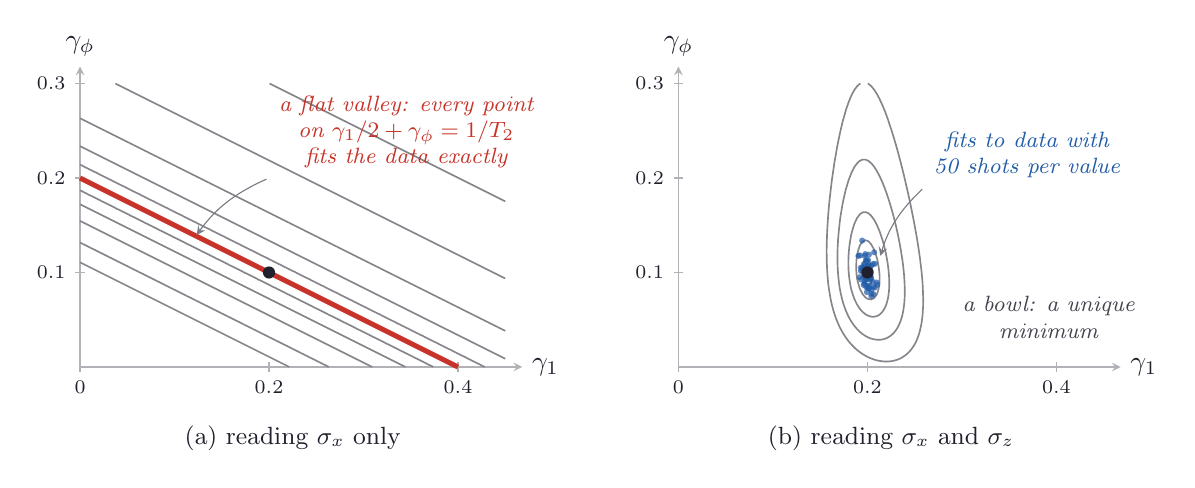
\begin{tikzpicture}[ink/.style={line width=0.9pt, ndInk}, faint/.style={line width=0.4pt, ndInk!35}, dashedink/.style={line width=0.5pt, ndInk!55, dash pattern=on 2.5pt off 2pt}, vec/.style={->, >=stealth, line width=1.2pt}, note/.style={font=\footnotesize\itshape, text=ndInk!85, align=center}, pointer/.style={->, >=stealth, line width=0.4pt, ndInk!60, shorten >=2pt, shorten <=1pt}, dot/.style={circle, fill=ndInk, inner sep=0pt, minimum size=3.4pt}, wash/.style={fill=ndSky, fill opacity=0.55}, every node/.style={text=ndInk}]
\definecolor{ndInk}{rgb}{0.13,0.13,0.18}
\definecolor{ndPaper}{rgb}{0.99,0.96,0.88}
\definecolor{ndSky}{rgb}{0.84,0.91,0.98}
\definecolor{ndRose}{rgb}{0.98,0.86,0.84}
\definecolor{ndBlue}{rgb}{0.13,0.36,0.66}
\definecolor{ndRed}{rgb}{0.78,0.20,0.16}
\definecolor{ndGold}{rgb}{0.88,0.62,0.10}
\definecolor{ndGreen}{rgb}{0.18,0.52,0.30}
\draw[faint, ->, >=stealth] (0.000,0.000) -- (5.616,0.000) node[right, text=ndInk] {$\gamma_1$};
\draw[faint, ->, >=stealth] (0.000,0.000) -- (0.000,3.816) node[above, text=ndInk] {$\gamma_\phi$};
\draw[faint] (0.000,0.060) -- (0.000,-0.060) node[below, font=\scriptsize, text=ndInk] {$0$};
\draw[faint] (2.400,0.060) -- (2.400,-0.060) node[below, font=\scriptsize, text=ndInk] {$0.2$};
\draw[faint] (4.800,0.060) -- (4.800,-0.060) node[below, font=\scriptsize, text=ndInk] {$0.4$};
\draw[faint] (0.060,1.200) -- (-0.060,1.200) node[left, font=\scriptsize, text=ndInk] {$0.1$};
\draw[faint] (0.060,2.400) -- (-0.060,2.400) node[left, font=\scriptsize, text=ndInk] {$0.2$};
\draw[faint] (0.060,3.600) -- (-0.060,3.600) node[left, font=\scriptsize, text=ndInk] {$0.3$};
\draw[line width=0.6pt, ndInk!55] (4.487,0.000) -- (4.464,0.012) -- (4.428,0.029) -- (4.426,0.030) -- (4.392,0.048) -- (4.367,0.060) -- (4.356,0.066) -- (4.320,0.084) -- (4.307,0.090) -- (4.284,0.102) -- (4.248,0.119) -- (4.246,0.120) -- (4.212,0.138) -- (4.187,0.150) -- (4.176,0.156) -- (4.140,0.174) -- (4.127,0.180) -- (4.104,0.192) -- (4.068,0.209) -- (4.066,0.210) -- (4.032,0.228) -- (4.007,0.240) -- (3.996,0.246) -- (3.960,0.264) -- (3.947,0.270) -- (3.924,0.282) -- (3.888,0.299) -- (3.886,0.300) -- (3.852,0.318) -- (3.827,0.330) -- (3.816,0.336) -- (3.780,0.354) -- (3.767,0.360) -- (3.744,0.372) -- (3.708,0.389) -- (3.706,0.390) -- (3.672,0.408) -- (3.647,0.420) -- (3.636,0.426) -- (3.600,0.444) -- (3.587,0.450) -- (3.564,0.462) -- (3.528,0.479) -- (3.526,0.480) -- (3.492,0.498) -- (3.467,0.510) -- (3.456,0.516) -- (3.420,0.534) -- (3.407,0.540) -- (3.384,0.552) -- (3.348,0.569) -- (3.346,0.570) -- (3.312,0.588) -- (3.287,0.600) -- (3.276,0.606) -- (3.240,0.624) -- (3.227,0.630) -- (3.204,0.642) -- (3.168,0.659) -- (3.166,0.660) -- (3.132,0.678) -- (3.107,0.690) -- (3.096,0.696) -- (3.060,0.714) -- (3.047,0.720) -- (3.024,0.732) -- (2.988,0.749) -- (2.986,0.750) -- (2.952,0.768) -- (2.927,0.780) -- (2.916,0.786) -- (2.880,0.804) -- (2.867,0.810) -- (2.844,0.822) -- (2.808,0.839) -- (2.806,0.840) -- (2.772,0.858) -- (2.747,0.870) -- (2.736,0.876) -- (2.700,0.894) -- (2.687,0.900) -- (2.664,0.912) -- (2.628,0.929) -- (2.626,0.930) -- (2.592,0.948) -- (2.567,0.960) -- (2.556,0.966) -- (2.520,0.984) -- (2.507,0.990) -- (2.484,1.002) -- (2.448,1.019) -- (2.446,1.020) -- (2.412,1.038) -- (2.387,1.050) -- (2.376,1.056) -- (2.340,1.074) -- (2.327,1.080) -- (2.304,1.092) -- (2.268,1.109) -- (2.266,1.110) -- (2.232,1.128) -- (2.207,1.140) -- (2.196,1.146) -- (2.160,1.164) -- (2.147,1.170) -- (2.124,1.182) -- (2.088,1.199) -- (2.086,1.200) -- (2.052,1.218) -- (2.027,1.230) -- (2.016,1.236) -- (1.980,1.254) -- (1.967,1.260) -- (1.944,1.272) -- (1.908,1.289) -- (1.906,1.290) -- (1.872,1.308) -- (1.847,1.320) -- (1.836,1.326) -- (1.800,1.344) -- (1.787,1.350) -- (1.764,1.362) -- (1.728,1.379) -- (1.726,1.380) -- (1.692,1.398) -- (1.667,1.410) -- (1.656,1.416) -- (1.620,1.434) -- (1.607,1.440) -- (1.584,1.452) -- (1.548,1.469) -- (1.546,1.470) -- (1.512,1.488) -- (1.487,1.500) -- (1.476,1.506) -- (1.440,1.524) -- (1.427,1.530) -- (1.404,1.542) -- (1.368,1.559) -- (1.366,1.560) -- (1.332,1.578) -- (1.307,1.590) -- (1.296,1.596) -- (1.260,1.614) -- (1.247,1.620) -- (1.224,1.632) -- (1.188,1.649) -- (1.186,1.650) -- (1.152,1.668) -- (1.127,1.680) -- (1.116,1.686) -- (1.080,1.704) -- (1.067,1.710) -- (1.044,1.722) -- (1.008,1.739) -- (1.006,1.740) -- (0.972,1.758) -- (0.947,1.770) -- (0.936,1.776) -- (0.900,1.794) -- (0.887,1.800) -- (0.864,1.812) -- (0.828,1.829) -- (0.826,1.830) -- (0.792,1.848) -- (0.767,1.860) -- (0.756,1.866) -- (0.720,1.884) -- (0.707,1.890) -- (0.684,1.902) -- (0.648,1.919) -- (0.646,1.920) -- (0.612,1.938) -- (0.587,1.950) -- (0.576,1.956) -- (0.540,1.974) -- (0.527,1.980) -- (0.504,1.992) -- (0.468,2.009) -- (0.466,2.010) -- (0.432,2.028) -- (0.407,2.040) -- (0.396,2.046) -- (0.360,2.064) -- (0.347,2.070) -- (0.324,2.082) -- (0.288,2.099) -- (0.286,2.100) -- (0.252,2.118) -- (0.227,2.130) -- (0.216,2.136) -- (0.180,2.154) -- (0.167,2.160) -- (0.144,2.172) -- (0.108,2.189) -- (0.106,2.190) -- (0.072,2.208) -- (0.047,2.220) -- (0.036,2.226) -- (0.000,2.244);
\draw[line width=0.6pt, ndInk!55] (0.000,2.570) -- (0.036,2.553) -- (0.041,2.550) -- (0.072,2.534) -- (0.101,2.520) -- (0.108,2.516) -- (0.144,2.498) -- (0.161,2.490) -- (0.180,2.480) -- (0.216,2.463) -- (0.221,2.460) -- (0.252,2.444) -- (0.281,2.430) -- (0.288,2.426) -- (0.324,2.408) -- (0.341,2.400) -- (0.360,2.390) -- (0.396,2.373) -- (0.401,2.370) -- (0.432,2.354) -- (0.461,2.340) -- (0.468,2.336) -- (0.504,2.318) -- (0.521,2.310) -- (0.540,2.300) -- (0.576,2.283) -- (0.581,2.280) -- (0.612,2.264) -- (0.641,2.250) -- (0.648,2.246) -- (0.684,2.228) -- (0.701,2.220) -- (0.720,2.210) -- (0.756,2.193) -- (0.761,2.190) -- (0.792,2.174) -- (0.821,2.160) -- (0.828,2.156) -- (0.864,2.138) -- (0.881,2.130) -- (0.900,2.120) -- (0.936,2.103) -- (0.941,2.100) -- (0.972,2.084) -- (1.001,2.070) -- (1.008,2.066) -- (1.044,2.048) -- (1.061,2.040) -- (1.080,2.030) -- (1.116,2.013) -- (1.121,2.010) -- (1.152,1.994) -- (1.181,1.980) -- (1.188,1.976) -- (1.224,1.958) -- (1.241,1.950) -- (1.260,1.940) -- (1.296,1.923) -- (1.301,1.920) -- (1.332,1.904) -- (1.361,1.890) -- (1.368,1.886) -- (1.404,1.868) -- (1.421,1.860) -- (1.440,1.850) -- (1.476,1.833) -- (1.481,1.830) -- (1.512,1.814) -- (1.541,1.800) -- (1.548,1.796) -- (1.584,1.778) -- (1.601,1.770) -- (1.620,1.760) -- (1.656,1.743) -- (1.661,1.740) -- (1.692,1.724) -- (1.721,1.710) -- (1.728,1.706) -- (1.764,1.688) -- (1.781,1.680) -- (1.800,1.670) -- (1.836,1.653) -- (1.841,1.650) -- (1.872,1.634) -- (1.901,1.620) -- (1.908,1.616) -- (1.944,1.598) -- (1.961,1.590) -- (1.980,1.580) -- (2.016,1.563) -- (2.021,1.560) -- (2.052,1.544) -- (2.081,1.530) -- (2.088,1.526) -- (2.124,1.508) -- (2.141,1.500) -- (2.160,1.490) -- (2.196,1.473) -- (2.201,1.470) -- (2.232,1.454) -- (2.261,1.440) -- (2.268,1.436) -- (2.304,1.418) -- (2.321,1.410) -- (2.340,1.400) -- (2.376,1.383) -- (2.381,1.380) -- (2.412,1.364) -- (2.441,1.350) -- (2.448,1.346) -- (2.484,1.328) -- (2.501,1.320) -- (2.520,1.310) -- (2.556,1.293) -- (2.561,1.290) -- (2.592,1.274) -- (2.621,1.260) -- (2.628,1.256) -- (2.664,1.238) -- (2.681,1.230) -- (2.700,1.220) -- (2.736,1.203) -- (2.741,1.200) -- (2.772,1.184) -- (2.801,1.170) -- (2.808,1.166) -- (2.844,1.148) -- (2.861,1.140) -- (2.880,1.130) -- (2.916,1.113) -- (2.921,1.110) -- (2.952,1.094) -- (2.981,1.080) -- (2.988,1.076) -- (3.024,1.058) -- (3.041,1.050) -- (3.060,1.040) -- (3.096,1.023) -- (3.101,1.020) -- (3.132,1.004) -- (3.161,0.990) -- (3.168,0.986) -- (3.204,0.968) -- (3.221,0.960) -- (3.240,0.950) -- (3.276,0.933) -- (3.281,0.930) -- (3.312,0.914) -- (3.341,0.900) -- (3.348,0.896) -- (3.384,0.878) -- (3.401,0.870) -- (3.420,0.860) -- (3.456,0.843) -- (3.461,0.840) -- (3.492,0.824) -- (3.521,0.810) -- (3.528,0.806) -- (3.564,0.788) -- (3.581,0.780) -- (3.600,0.770) -- (3.636,0.753) -- (3.641,0.750) -- (3.672,0.734) -- (3.701,0.720) -- (3.708,0.716) -- (3.744,0.698) -- (3.761,0.690) -- (3.780,0.680) -- (3.816,0.663) -- (3.821,0.660) -- (3.852,0.644) -- (3.881,0.630) -- (3.888,0.626) -- (3.924,0.608) -- (3.941,0.600) -- (3.960,0.590) -- (3.996,0.573) -- (4.001,0.570) -- (4.032,0.554) -- (4.061,0.540) -- (4.068,0.536) -- (4.104,0.518) -- (4.121,0.510) -- (4.140,0.500) -- (4.176,0.483) -- (4.181,0.480) -- (4.212,0.464) -- (4.241,0.450) -- (4.248,0.446) -- (4.284,0.428) -- (4.301,0.420) -- (4.320,0.410) -- (4.356,0.393) -- (4.361,0.390) -- (4.392,0.374) -- (4.421,0.360) -- (4.428,0.356) -- (4.464,0.338) -- (4.481,0.330) -- (4.500,0.320) -- (4.536,0.303) -- (4.541,0.300) -- (4.572,0.284) -- (4.601,0.270) -- (4.608,0.266) -- (4.644,0.248) -- (4.661,0.240) -- (4.680,0.230) -- (4.716,0.213) -- (4.721,0.210) -- (4.752,0.194) -- (4.781,0.180) -- (4.788,0.176) -- (4.824,0.158) -- (4.841,0.150) -- (4.860,0.140) -- (4.896,0.123) -- (4.901,0.120) -- (4.932,0.104) -- (4.961,0.090) -- (4.968,0.086) -- (5.004,0.068) -- (5.021,0.060) -- (5.040,0.050) -- (5.076,0.033) -- (5.081,0.030) -- (5.112,0.014) -- (5.141,0.000);
\draw[line width=0.6pt, ndInk!55] (4.132,0.000) -- (4.104,0.014) -- (4.072,0.030) -- (4.068,0.032) -- (4.032,0.050) -- (4.012,0.060) -- (3.996,0.068) -- (3.960,0.086) -- (3.952,0.090) -- (3.924,0.104) -- (3.892,0.120) -- (3.888,0.122) -- (3.852,0.140) -- (3.832,0.150) -- (3.816,0.158) -- (3.780,0.176) -- (3.772,0.180) -- (3.744,0.194) -- (3.712,0.210) -- (3.708,0.212) -- (3.672,0.230) -- (3.652,0.240) -- (3.636,0.248) -- (3.600,0.266) -- (3.592,0.270) -- (3.564,0.284) -- (3.532,0.300) -- (3.528,0.302) -- (3.492,0.320) -- (3.472,0.330) -- (3.456,0.338) -- (3.420,0.356) -- (3.412,0.360) -- (3.384,0.374) -- (3.352,0.390) -- (3.348,0.392) -- (3.312,0.410) -- (3.292,0.420) -- (3.276,0.428) -- (3.240,0.446) -- (3.232,0.450) -- (3.204,0.464) -- (3.172,0.480) -- (3.168,0.482) -- (3.132,0.500) -- (3.112,0.510) -- (3.096,0.518) -- (3.060,0.536) -- (3.052,0.540) -- (3.024,0.554) -- (2.992,0.570) -- (2.988,0.572) -- (2.952,0.590) -- (2.932,0.600) -- (2.916,0.608) -- (2.880,0.626) -- (2.872,0.630) -- (2.844,0.644) -- (2.812,0.660) -- (2.808,0.662) -- (2.772,0.680) -- (2.752,0.690) -- (2.736,0.698) -- (2.700,0.716) -- (2.692,0.720) -- (2.664,0.734) -- (2.632,0.750) -- (2.628,0.752) -- (2.592,0.770) -- (2.572,0.780) -- (2.556,0.788) -- (2.520,0.806) -- (2.512,0.810) -- (2.484,0.824) -- (2.452,0.840) -- (2.448,0.842) -- (2.412,0.860) -- (2.392,0.870) -- (2.376,0.878) -- (2.340,0.896) -- (2.332,0.900) -- (2.304,0.914) -- (2.272,0.930) -- (2.268,0.932) -- (2.232,0.950) -- (2.212,0.960) -- (2.196,0.968) -- (2.160,0.986) -- (2.152,0.990) -- (2.124,1.004) -- (2.092,1.020) -- (2.088,1.022) -- (2.052,1.040) -- (2.032,1.050) -- (2.016,1.058) -- (1.980,1.076) -- (1.972,1.080) -- (1.944,1.094) -- (1.912,1.110) -- (1.908,1.112) -- (1.872,1.130) -- (1.852,1.140) -- (1.836,1.148) -- (1.800,1.166) -- (1.792,1.170) -- (1.764,1.184) -- (1.732,1.200) -- (1.728,1.202) -- (1.692,1.220) -- (1.672,1.230) -- (1.656,1.238) -- (1.620,1.256) -- (1.612,1.260) -- (1.584,1.274) -- (1.552,1.290) -- (1.548,1.292) -- (1.512,1.310) -- (1.492,1.320) -- (1.476,1.328) -- (1.440,1.346) -- (1.432,1.350) -- (1.404,1.364) -- (1.372,1.380) -- (1.368,1.382) -- (1.332,1.400) -- (1.312,1.410) -- (1.296,1.418) -- (1.260,1.436) -- (1.252,1.440) -- (1.224,1.454) -- (1.192,1.470) -- (1.188,1.472) -- (1.152,1.490) -- (1.132,1.500) -- (1.116,1.508) -- (1.080,1.526) -- (1.072,1.530) -- (1.044,1.544) -- (1.012,1.560) -- (1.008,1.562) -- (0.972,1.580) -- (0.952,1.590) -- (0.936,1.598) -- (0.900,1.616) -- (0.892,1.620) -- (0.864,1.634) -- (0.832,1.650) -- (0.828,1.652) -- (0.792,1.670) -- (0.772,1.680) -- (0.756,1.688) -- (0.720,1.706) -- (0.712,1.710) -- (0.684,1.724) -- (0.652,1.740) -- (0.648,1.742) -- (0.612,1.760) -- (0.592,1.770) -- (0.576,1.778) -- (0.540,1.796) -- (0.532,1.800) -- (0.504,1.814) -- (0.472,1.830) -- (0.468,1.832) -- (0.432,1.850) -- (0.412,1.860) -- (0.396,1.868) -- (0.360,1.886) -- (0.352,1.890) -- (0.324,1.904) -- (0.292,1.920) -- (0.288,1.922) -- (0.252,1.940) -- (0.232,1.950) -- (0.216,1.958) -- (0.180,1.976) -- (0.172,1.980) -- (0.144,1.994) -- (0.112,2.010) -- (0.108,2.012) -- (0.072,2.030) -- (0.052,2.040) -- (0.036,2.048) -- (0.000,2.066);
\draw[line width=0.6pt, ndInk!55] (0.000,2.804) -- (0.028,2.790) -- (0.036,2.786) -- (0.072,2.768) -- (0.088,2.760) -- (0.108,2.750) -- (0.144,2.732) -- (0.148,2.730) -- (0.180,2.714) -- (0.208,2.700) -- (0.216,2.696) -- (0.252,2.678) -- (0.268,2.670) -- (0.288,2.660) -- (0.324,2.642) -- (0.328,2.640) -- (0.360,2.624) -- (0.388,2.610) -- (0.396,2.606) -- (0.432,2.588) -- (0.448,2.580) -- (0.468,2.570) -- (0.504,2.552) -- (0.508,2.550) -- (0.540,2.534) -- (0.568,2.520) -- (0.576,2.516) -- (0.612,2.498) -- (0.628,2.490) -- (0.648,2.480) -- (0.684,2.462) -- (0.688,2.460) -- (0.720,2.444) -- (0.748,2.430) -- (0.756,2.426) -- (0.792,2.408) -- (0.808,2.400) -- (0.828,2.390) -- (0.864,2.372) -- (0.868,2.370) -- (0.900,2.354) -- (0.928,2.340) -- (0.936,2.336) -- (0.972,2.318) -- (0.988,2.310) -- (1.008,2.300) -- (1.044,2.282) -- (1.048,2.280) -- (1.080,2.264) -- (1.108,2.250) -- (1.116,2.246) -- (1.152,2.228) -- (1.168,2.220) -- (1.188,2.210) -- (1.224,2.192) -- (1.228,2.190) -- (1.260,2.174) -- (1.288,2.160) -- (1.296,2.156) -- (1.332,2.138) -- (1.348,2.130) -- (1.368,2.120) -- (1.404,2.102) -- (1.408,2.100) -- (1.440,2.084) -- (1.468,2.070) -- (1.476,2.066) -- (1.512,2.048) -- (1.528,2.040) -- (1.548,2.030) -- (1.584,2.012) -- (1.588,2.010) -- (1.620,1.994) -- (1.648,1.980) -- (1.656,1.976) -- (1.692,1.958) -- (1.708,1.950) -- (1.728,1.940) -- (1.764,1.922) -- (1.768,1.920) -- (1.800,1.904) -- (1.828,1.890) -- (1.836,1.886) -- (1.872,1.868) -- (1.888,1.860) -- (1.908,1.850) -- (1.944,1.832) -- (1.948,1.830) -- (1.980,1.814) -- (2.008,1.800) -- (2.016,1.796) -- (2.052,1.778) -- (2.068,1.770) -- (2.088,1.760) -- (2.124,1.742) -- (2.128,1.740) -- (2.160,1.724) -- (2.188,1.710) -- (2.196,1.706) -- (2.232,1.688) -- (2.248,1.680) -- (2.268,1.670) -- (2.304,1.652) -- (2.308,1.650) -- (2.340,1.634) -- (2.368,1.620) -- (2.376,1.616) -- (2.412,1.598) -- (2.428,1.590) -- (2.448,1.580) -- (2.484,1.562) -- (2.488,1.560) -- (2.520,1.544) -- (2.548,1.530) -- (2.556,1.526) -- (2.592,1.508) -- (2.608,1.500) -- (2.628,1.490) -- (2.664,1.472) -- (2.668,1.470) -- (2.700,1.454) -- (2.728,1.440) -- (2.736,1.436) -- (2.772,1.418) -- (2.788,1.410) -- (2.808,1.400) -- (2.844,1.382) -- (2.848,1.380) -- (2.880,1.364) -- (2.908,1.350) -- (2.916,1.346) -- (2.952,1.328) -- (2.968,1.320) -- (2.988,1.310) -- (3.024,1.292) -- (3.028,1.290) -- (3.060,1.274) -- (3.088,1.260) -- (3.096,1.256) -- (3.132,1.238) -- (3.148,1.230) -- (3.168,1.220) -- (3.204,1.202) -- (3.208,1.200) -- (3.240,1.184) -- (3.268,1.170) -- (3.276,1.166) -- (3.312,1.148) -- (3.328,1.140) -- (3.348,1.130) -- (3.384,1.112) -- (3.388,1.110) -- (3.420,1.094) -- (3.448,1.080) -- (3.456,1.076) -- (3.492,1.058) -- (3.508,1.050) -- (3.528,1.040) -- (3.564,1.022) -- (3.568,1.020) -- (3.600,1.004) -- (3.628,0.990) -- (3.636,0.986) -- (3.672,0.968) -- (3.688,0.960) -- (3.708,0.950) -- (3.744,0.932) -- (3.748,0.930) -- (3.780,0.914) -- (3.808,0.900) -- (3.816,0.896) -- (3.852,0.878) -- (3.868,0.870) -- (3.888,0.860) -- (3.924,0.842) -- (3.928,0.840) -- (3.960,0.824) -- (3.988,0.810) -- (3.996,0.806) -- (4.032,0.788) -- (4.048,0.780) -- (4.068,0.770) -- (4.104,0.752) -- (4.108,0.750) -- (4.140,0.734) -- (4.168,0.720) -- (4.176,0.716) -- (4.212,0.698) -- (4.228,0.690) -- (4.248,0.680) -- (4.284,0.662) -- (4.288,0.660) -- (4.320,0.644) -- (4.348,0.630) -- (4.356,0.626) -- (4.392,0.608) -- (4.408,0.600) -- (4.428,0.590) -- (4.464,0.572) -- (4.468,0.570) -- (4.500,0.554) -- (4.528,0.540) -- (4.536,0.536) -- (4.572,0.518) -- (4.588,0.510) -- (4.608,0.500) -- (4.644,0.482) -- (4.648,0.480) -- (4.680,0.464) -- (4.708,0.450) -- (4.716,0.446) -- (4.752,0.428) -- (4.768,0.420) -- (4.788,0.410) -- (4.824,0.392) -- (4.828,0.390) -- (4.860,0.374) -- (4.888,0.360) -- (4.896,0.356) -- (4.932,0.338) -- (4.948,0.330) -- (4.968,0.320) -- (5.004,0.302) -- (5.008,0.300) -- (5.040,0.284) -- (5.068,0.270) -- (5.076,0.266) -- (5.112,0.248) -- (5.128,0.240) -- (5.148,0.230) -- (5.184,0.212) -- (5.188,0.210) -- (5.220,0.194) -- (5.248,0.180) -- (5.256,0.176) -- (5.292,0.158) -- (5.308,0.150) -- (5.328,0.140) -- (5.364,0.122) -- (5.368,0.120) -- (5.400,0.104);
\draw[line width=0.6pt, ndInk!55] (3.710,0.000) -- (3.708,0.001) -- (3.672,0.019) -- (3.650,0.030) -- (3.636,0.037) -- (3.600,0.055) -- (3.590,0.060) -- (3.564,0.073) -- (3.530,0.090) -- (3.528,0.091) -- (3.492,0.109) -- (3.470,0.120) -- (3.456,0.127) -- (3.420,0.145) -- (3.410,0.150) -- (3.384,0.163) -- (3.350,0.180) -- (3.348,0.181) -- (3.312,0.199) -- (3.290,0.210) -- (3.276,0.217) -- (3.240,0.235) -- (3.230,0.240) -- (3.204,0.253) -- (3.170,0.270) -- (3.168,0.271) -- (3.132,0.289) -- (3.110,0.300) -- (3.096,0.307) -- (3.060,0.325) -- (3.050,0.330) -- (3.024,0.343) -- (2.990,0.360) -- (2.988,0.361) -- (2.952,0.379) -- (2.930,0.390) -- (2.916,0.397) -- (2.880,0.415) -- (2.870,0.420) -- (2.844,0.433) -- (2.810,0.450) -- (2.808,0.451) -- (2.772,0.469) -- (2.750,0.480) -- (2.736,0.487) -- (2.700,0.505) -- (2.690,0.510) -- (2.664,0.523) -- (2.630,0.540) -- (2.628,0.541) -- (2.592,0.559) -- (2.570,0.570) -- (2.556,0.577) -- (2.520,0.595) -- (2.510,0.600) -- (2.484,0.613) -- (2.450,0.630) -- (2.448,0.631) -- (2.412,0.649) -- (2.390,0.660) -- (2.376,0.667) -- (2.340,0.685) -- (2.330,0.690) -- (2.304,0.703) -- (2.270,0.720) -- (2.268,0.721) -- (2.232,0.739) -- (2.210,0.750) -- (2.196,0.757) -- (2.160,0.775) -- (2.150,0.780) -- (2.124,0.793) -- (2.090,0.810) -- (2.088,0.811) -- (2.052,0.829) -- (2.030,0.840) -- (2.016,0.847) -- (1.980,0.865) -- (1.970,0.870) -- (1.944,0.883) -- (1.910,0.900) -- (1.908,0.901) -- (1.872,0.919) -- (1.850,0.930) -- (1.836,0.937) -- (1.800,0.955) -- (1.790,0.960) -- (1.764,0.973) -- (1.730,0.990) -- (1.728,0.991) -- (1.692,1.009) -- (1.670,1.020) -- (1.656,1.027) -- (1.620,1.045) -- (1.610,1.050) -- (1.584,1.063) -- (1.550,1.080) -- (1.548,1.081) -- (1.512,1.099) -- (1.490,1.110) -- (1.476,1.117) -- (1.440,1.135) -- (1.430,1.140) -- (1.404,1.153) -- (1.370,1.170) -- (1.368,1.171) -- (1.332,1.189) -- (1.310,1.200) -- (1.296,1.207) -- (1.260,1.225) -- (1.250,1.230) -- (1.224,1.243) -- (1.190,1.260) -- (1.188,1.261) -- (1.152,1.279) -- (1.130,1.290) -- (1.116,1.297) -- (1.080,1.315) -- (1.070,1.320) -- (1.044,1.333) -- (1.010,1.350) -- (1.008,1.351) -- (0.972,1.369) -- (0.950,1.380) -- (0.936,1.387) -- (0.900,1.405) -- (0.890,1.410) -- (0.864,1.423) -- (0.830,1.440) -- (0.828,1.441) -- (0.792,1.459) -- (0.770,1.470) -- (0.756,1.477) -- (0.720,1.495) -- (0.710,1.500) -- (0.684,1.513) -- (0.650,1.530) -- (0.648,1.531) -- (0.612,1.549) -- (0.590,1.560) -- (0.576,1.567) -- (0.540,1.585) -- (0.530,1.590) -- (0.504,1.603) -- (0.470,1.620) -- (0.468,1.621) -- (0.432,1.639) -- (0.410,1.650) -- (0.396,1.657) -- (0.360,1.675) -- (0.350,1.680) -- (0.324,1.693) -- (0.290,1.710) -- (0.288,1.711) -- (0.252,1.729) -- (0.230,1.740) -- (0.216,1.747) -- (0.180,1.765) -- (0.170,1.770) -- (0.144,1.783) -- (0.110,1.800) -- (0.108,1.801) -- (0.072,1.819) -- (0.050,1.830) -- (0.036,1.837) -- (0.000,1.855);
\draw[line width=0.6pt, ndInk!55] (0.000,3.159) -- (0.019,3.150) -- (0.036,3.141) -- (0.072,3.123) -- (0.079,3.120) -- (0.108,3.105) -- (0.139,3.090) -- (0.144,3.087) -- (0.180,3.069) -- (0.199,3.060) -- (0.216,3.051) -- (0.252,3.033) -- (0.259,3.030) -- (0.288,3.015) -- (0.319,3.000) -- (0.324,2.997) -- (0.360,2.979) -- (0.379,2.970) -- (0.396,2.961) -- (0.432,2.943) -- (0.439,2.940) -- (0.468,2.925) -- (0.499,2.910) -- (0.504,2.907) -- (0.540,2.889) -- (0.559,2.880) -- (0.576,2.871) -- (0.612,2.853) -- (0.619,2.850) -- (0.648,2.835) -- (0.679,2.820) -- (0.684,2.817) -- (0.720,2.799) -- (0.739,2.790) -- (0.756,2.781) -- (0.792,2.763) -- (0.799,2.760) -- (0.828,2.745) -- (0.859,2.730) -- (0.864,2.727) -- (0.900,2.709) -- (0.919,2.700) -- (0.936,2.691) -- (0.972,2.673) -- (0.979,2.670) -- (1.008,2.655) -- (1.039,2.640) -- (1.044,2.637) -- (1.080,2.619) -- (1.099,2.610) -- (1.116,2.601) -- (1.152,2.583) -- (1.159,2.580) -- (1.188,2.565) -- (1.219,2.550) -- (1.224,2.547) -- (1.260,2.529) -- (1.279,2.520) -- (1.296,2.511) -- (1.332,2.493) -- (1.339,2.490) -- (1.368,2.475) -- (1.399,2.460) -- (1.404,2.457) -- (1.440,2.439) -- (1.459,2.430) -- (1.476,2.421) -- (1.512,2.403) -- (1.519,2.400) -- (1.548,2.385) -- (1.579,2.370) -- (1.584,2.367) -- (1.620,2.349) -- (1.639,2.340) -- (1.656,2.331) -- (1.692,2.313) -- (1.699,2.310) -- (1.728,2.295) -- (1.759,2.280) -- (1.764,2.277) -- (1.800,2.259) -- (1.819,2.250) -- (1.836,2.241) -- (1.872,2.223) -- (1.879,2.220) -- (1.908,2.205) -- (1.939,2.190) -- (1.944,2.187) -- (1.980,2.169) -- (1.999,2.160) -- (2.016,2.151) -- (2.052,2.133) -- (2.059,2.130) -- (2.088,2.115) -- (2.119,2.100) -- (2.124,2.097) -- (2.160,2.079) -- (2.179,2.070) -- (2.196,2.061) -- (2.232,2.043) -- (2.239,2.040) -- (2.268,2.025) -- (2.299,2.010) -- (2.304,2.007) -- (2.340,1.989) -- (2.359,1.980) -- (2.376,1.971) -- (2.412,1.953) -- (2.419,1.950) -- (2.448,1.935) -- (2.479,1.920) -- (2.484,1.917) -- (2.520,1.899) -- (2.539,1.890) -- (2.556,1.881) -- (2.592,1.863) -- (2.599,1.860) -- (2.628,1.845) -- (2.659,1.830) -- (2.664,1.827) -- (2.700,1.809) -- (2.719,1.800) -- (2.736,1.791) -- (2.772,1.773) -- (2.779,1.770) -- (2.808,1.755) -- (2.839,1.740) -- (2.844,1.737) -- (2.880,1.719) -- (2.899,1.710) -- (2.916,1.701) -- (2.952,1.683) -- (2.959,1.680) -- (2.988,1.665) -- (3.019,1.650) -- (3.024,1.647) -- (3.060,1.629) -- (3.079,1.620) -- (3.096,1.611) -- (3.132,1.593) -- (3.139,1.590) -- (3.168,1.575) -- (3.199,1.560) -- (3.204,1.557) -- (3.240,1.539) -- (3.259,1.530) -- (3.276,1.521) -- (3.312,1.503) -- (3.319,1.500) -- (3.348,1.485) -- (3.379,1.470) -- (3.384,1.467) -- (3.420,1.449) -- (3.439,1.440) -- (3.456,1.431) -- (3.492,1.413) -- (3.499,1.410) -- (3.528,1.395) -- (3.559,1.380) -- (3.564,1.377) -- (3.600,1.359) -- (3.619,1.350) -- (3.636,1.341) -- (3.672,1.323) -- (3.679,1.320) -- (3.708,1.305) -- (3.739,1.290) -- (3.744,1.287) -- (3.780,1.269) -- (3.799,1.260) -- (3.816,1.251) -- (3.852,1.233) -- (3.859,1.230) -- (3.888,1.215) -- (3.919,1.200) -- (3.924,1.197) -- (3.960,1.179) -- (3.979,1.170) -- (3.996,1.161) -- (4.032,1.143) -- (4.039,1.140) -- (4.068,1.125) -- (4.099,1.110) -- (4.104,1.107) -- (4.140,1.089) -- (4.159,1.080) -- (4.176,1.071) -- (4.212,1.053) -- (4.219,1.050) -- (4.248,1.035) -- (4.279,1.020) -- (4.284,1.017) -- (4.320,0.999) -- (4.339,0.990) -- (4.356,0.981) -- (4.392,0.963) -- (4.399,0.960) -- (4.428,0.945) -- (4.459,0.930) -- (4.464,0.927) -- (4.500,0.909) -- (4.519,0.900) -- (4.536,0.891) -- (4.572,0.873) -- (4.579,0.870) -- (4.608,0.855) -- (4.639,0.840) -- (4.644,0.837) -- (4.680,0.819) -- (4.699,0.810) -- (4.716,0.801) -- (4.752,0.783) -- (4.759,0.780) -- (4.788,0.765) -- (4.819,0.750) -- (4.824,0.747) -- (4.860,0.729) -- (4.879,0.720) -- (4.896,0.711) -- (4.932,0.693) -- (4.939,0.690) -- (4.968,0.675) -- (4.999,0.660) -- (5.004,0.657) -- (5.040,0.639) -- (5.059,0.630) -- (5.076,0.621) -- (5.112,0.603) -- (5.119,0.600) -- (5.148,0.585) -- (5.179,0.570) -- (5.184,0.567) -- (5.220,0.549) -- (5.239,0.540) -- (5.256,0.531) -- (5.292,0.513) -- (5.299,0.510) -- (5.328,0.495) -- (5.359,0.480) -- (5.364,0.477) -- (5.400,0.459);
\draw[line width=0.6pt, ndInk!55] (3.160,0.000) -- (3.132,0.014) -- (3.100,0.030) -- (3.096,0.032) -- (3.060,0.050) -- (3.040,0.060) -- (3.024,0.068) -- (2.988,0.086) -- (2.980,0.090) -- (2.952,0.104) -- (2.920,0.120) -- (2.916,0.122) -- (2.880,0.140) -- (2.860,0.150) -- (2.844,0.158) -- (2.808,0.176) -- (2.800,0.180) -- (2.772,0.194) -- (2.740,0.210) -- (2.736,0.212) -- (2.700,0.230) -- (2.680,0.240) -- (2.664,0.248) -- (2.628,0.266) -- (2.620,0.270) -- (2.592,0.284) -- (2.560,0.300) -- (2.556,0.302) -- (2.520,0.320) -- (2.500,0.330) -- (2.484,0.338) -- (2.448,0.356) -- (2.440,0.360) -- (2.412,0.374) -- (2.380,0.390) -- (2.376,0.392) -- (2.340,0.410) -- (2.320,0.420) -- (2.304,0.428) -- (2.268,0.446) -- (2.260,0.450) -- (2.232,0.464) -- (2.200,0.480) -- (2.196,0.482) -- (2.160,0.500) -- (2.140,0.510) -- (2.124,0.518) -- (2.088,0.536) -- (2.080,0.540) -- (2.052,0.554) -- (2.020,0.570) -- (2.016,0.572) -- (1.980,0.590) -- (1.960,0.600) -- (1.944,0.608) -- (1.908,0.626) -- (1.900,0.630) -- (1.872,0.644) -- (1.840,0.660) -- (1.836,0.662) -- (1.800,0.680) -- (1.780,0.690) -- (1.764,0.698) -- (1.728,0.716) -- (1.720,0.720) -- (1.692,0.734) -- (1.660,0.750) -- (1.656,0.752) -- (1.620,0.770) -- (1.600,0.780) -- (1.584,0.788) -- (1.548,0.806) -- (1.540,0.810) -- (1.512,0.824) -- (1.480,0.840) -- (1.476,0.842) -- (1.440,0.860) -- (1.420,0.870) -- (1.404,0.878) -- (1.368,0.896) -- (1.360,0.900) -- (1.332,0.914) -- (1.300,0.930) -- (1.296,0.932) -- (1.260,0.950) -- (1.240,0.960) -- (1.224,0.968) -- (1.188,0.986) -- (1.180,0.990) -- (1.152,1.004) -- (1.120,1.020) -- (1.116,1.022) -- (1.080,1.040) -- (1.060,1.050) -- (1.044,1.058) -- (1.008,1.076) -- (1.000,1.080) -- (0.972,1.094) -- (0.940,1.110) -- (0.936,1.112) -- (0.900,1.130) -- (0.880,1.140) -- (0.864,1.148) -- (0.828,1.166) -- (0.820,1.170) -- (0.792,1.184) -- (0.760,1.200) -- (0.756,1.202) -- (0.720,1.220) -- (0.700,1.230) -- (0.684,1.238) -- (0.648,1.256) -- (0.640,1.260) -- (0.612,1.274) -- (0.580,1.290) -- (0.576,1.292) -- (0.540,1.310) -- (0.520,1.320) -- (0.504,1.328) -- (0.468,1.346) -- (0.460,1.350) -- (0.432,1.364) -- (0.400,1.380) -- (0.396,1.382) -- (0.360,1.400) -- (0.340,1.410) -- (0.324,1.418) -- (0.288,1.436) -- (0.280,1.440) -- (0.252,1.454) -- (0.220,1.470) -- (0.216,1.472) -- (0.180,1.490) -- (0.160,1.500) -- (0.144,1.508) -- (0.108,1.526) -- (0.100,1.530) -- (0.072,1.544) -- (0.040,1.560) -- (0.036,1.562) -- (0.000,1.580);
\draw[line width=0.6pt, ndInk!55] (0.449,3.600) -- (0.468,3.590) -- (0.504,3.572) -- (0.509,3.570) -- (0.540,3.554) -- (0.569,3.540) -- (0.576,3.536) -- (0.612,3.518) -- (0.629,3.510) -- (0.648,3.500) -- (0.684,3.482) -- (0.689,3.480) -- (0.720,3.464) -- (0.749,3.450) -- (0.756,3.446) -- (0.792,3.428) -- (0.809,3.420) -- (0.828,3.410) -- (0.864,3.392) -- (0.869,3.390) -- (0.900,3.374) -- (0.929,3.360) -- (0.936,3.356) -- (0.972,3.338) -- (0.989,3.330) -- (1.008,3.320) -- (1.044,3.302) -- (1.049,3.300) -- (1.080,3.284) -- (1.109,3.270) -- (1.116,3.266) -- (1.152,3.248) -- (1.169,3.240) -- (1.188,3.230) -- (1.224,3.212) -- (1.229,3.210) -- (1.260,3.194) -- (1.289,3.180) -- (1.296,3.176) -- (1.332,3.158) -- (1.349,3.150) -- (1.368,3.140) -- (1.404,3.122) -- (1.409,3.120) -- (1.440,3.104) -- (1.469,3.090) -- (1.476,3.086) -- (1.512,3.068) -- (1.529,3.060) -- (1.548,3.050) -- (1.584,3.032) -- (1.589,3.030) -- (1.620,3.014) -- (1.649,3.000) -- (1.656,2.996) -- (1.692,2.978) -- (1.709,2.970) -- (1.728,2.960) -- (1.764,2.942) -- (1.769,2.940) -- (1.800,2.924) -- (1.829,2.910) -- (1.836,2.906) -- (1.872,2.888) -- (1.889,2.880) -- (1.908,2.870) -- (1.944,2.852) -- (1.949,2.850) -- (1.980,2.834) -- (2.009,2.820) -- (2.016,2.816) -- (2.052,2.798) -- (2.069,2.790) -- (2.088,2.780) -- (2.124,2.762) -- (2.129,2.760) -- (2.160,2.744) -- (2.189,2.730) -- (2.196,2.726) -- (2.232,2.708) -- (2.249,2.700) -- (2.268,2.690) -- (2.304,2.672) -- (2.309,2.670) -- (2.340,2.654) -- (2.369,2.640) -- (2.376,2.636) -- (2.412,2.618) -- (2.429,2.610) -- (2.448,2.600) -- (2.484,2.582) -- (2.489,2.580) -- (2.520,2.564) -- (2.549,2.550) -- (2.556,2.546) -- (2.592,2.528) -- (2.609,2.520) -- (2.628,2.510) -- (2.664,2.492) -- (2.669,2.490) -- (2.700,2.474) -- (2.729,2.460) -- (2.736,2.456) -- (2.772,2.438) -- (2.789,2.430) -- (2.808,2.420) -- (2.844,2.402) -- (2.849,2.400) -- (2.880,2.384) -- (2.909,2.370) -- (2.916,2.366) -- (2.952,2.348) -- (2.969,2.340) -- (2.988,2.330) -- (3.024,2.312) -- (3.029,2.310) -- (3.060,2.294) -- (3.089,2.280) -- (3.096,2.276) -- (3.132,2.258) -- (3.149,2.250) -- (3.168,2.240) -- (3.204,2.222) -- (3.209,2.220) -- (3.240,2.204) -- (3.269,2.190) -- (3.276,2.186) -- (3.312,2.168) -- (3.329,2.160) -- (3.348,2.150) -- (3.384,2.132) -- (3.389,2.130) -- (3.420,2.114) -- (3.449,2.100) -- (3.456,2.096) -- (3.492,2.078) -- (3.509,2.070) -- (3.528,2.060) -- (3.564,2.042) -- (3.569,2.040) -- (3.600,2.024) -- (3.629,2.010) -- (3.636,2.006) -- (3.672,1.988) -- (3.689,1.980) -- (3.708,1.970) -- (3.744,1.952) -- (3.749,1.950) -- (3.780,1.934) -- (3.809,1.920) -- (3.816,1.916) -- (3.852,1.898) -- (3.869,1.890) -- (3.888,1.880) -- (3.924,1.862) -- (3.929,1.860) -- (3.960,1.844) -- (3.989,1.830) -- (3.996,1.826) -- (4.032,1.808) -- (4.049,1.800) -- (4.068,1.790) -- (4.104,1.772) -- (4.109,1.770) -- (4.140,1.754) -- (4.169,1.740) -- (4.176,1.736) -- (4.212,1.718) -- (4.229,1.710) -- (4.248,1.700) -- (4.284,1.682) -- (4.289,1.680) -- (4.320,1.664) -- (4.349,1.650) -- (4.356,1.646) -- (4.392,1.628) -- (4.409,1.620) -- (4.428,1.610) -- (4.464,1.592) -- (4.469,1.590) -- (4.500,1.574) -- (4.529,1.560) -- (4.536,1.556) -- (4.572,1.538) -- (4.589,1.530) -- (4.608,1.520) -- (4.644,1.502) -- (4.649,1.500) -- (4.680,1.484) -- (4.709,1.470) -- (4.716,1.466) -- (4.752,1.448) -- (4.769,1.440) -- (4.788,1.430) -- (4.824,1.412) -- (4.829,1.410) -- (4.860,1.394) -- (4.889,1.380) -- (4.896,1.376) -- (4.932,1.358) -- (4.949,1.350) -- (4.968,1.340) -- (5.004,1.322) -- (5.009,1.320) -- (5.040,1.304) -- (5.069,1.290) -- (5.076,1.286) -- (5.112,1.268) -- (5.129,1.260) -- (5.148,1.250) -- (5.184,1.232) -- (5.189,1.230) -- (5.220,1.214) -- (5.249,1.200) -- (5.256,1.196) -- (5.292,1.178) -- (5.309,1.170) -- (5.328,1.160) -- (5.364,1.142) -- (5.369,1.140) -- (5.400,1.124);
\draw[line width=0.6pt, ndInk!55] (2.658,0.000) -- (2.628,0.015) -- (2.598,0.030) -- (2.592,0.033) -- (2.556,0.051) -- (2.538,0.060) -- (2.520,0.069) -- (2.484,0.087) -- (2.478,0.090) -- (2.448,0.105) -- (2.418,0.120) -- (2.412,0.123) -- (2.376,0.141) -- (2.358,0.150) -- (2.340,0.159) -- (2.304,0.177) -- (2.298,0.180) -- (2.268,0.195) -- (2.238,0.210) -- (2.232,0.213) -- (2.196,0.231) -- (2.178,0.240) -- (2.160,0.249) -- (2.124,0.267) -- (2.118,0.270) -- (2.088,0.285) -- (2.058,0.300) -- (2.052,0.303) -- (2.016,0.321) -- (1.998,0.330) -- (1.980,0.339) -- (1.944,0.357) -- (1.938,0.360) -- (1.908,0.375) -- (1.878,0.390) -- (1.872,0.393) -- (1.836,0.411) -- (1.818,0.420) -- (1.800,0.429) -- (1.764,0.447) -- (1.758,0.450) -- (1.728,0.465) -- (1.698,0.480) -- (1.692,0.483) -- (1.656,0.501) -- (1.638,0.510) -- (1.620,0.519) -- (1.584,0.537) -- (1.578,0.540) -- (1.548,0.555) -- (1.518,0.570) -- (1.512,0.573) -- (1.476,0.591) -- (1.458,0.600) -- (1.440,0.609) -- (1.404,0.627) -- (1.398,0.630) -- (1.368,0.645) -- (1.338,0.660) -- (1.332,0.663) -- (1.296,0.681) -- (1.278,0.690) -- (1.260,0.699) -- (1.224,0.717) -- (1.218,0.720) -- (1.188,0.735) -- (1.158,0.750) -- (1.152,0.753) -- (1.116,0.771) -- (1.098,0.780) -- (1.080,0.789) -- (1.044,0.807) -- (1.038,0.810) -- (1.008,0.825) -- (0.978,0.840) -- (0.972,0.843) -- (0.936,0.861) -- (0.918,0.870) -- (0.900,0.879) -- (0.864,0.897) -- (0.858,0.900) -- (0.828,0.915) -- (0.798,0.930) -- (0.792,0.933) -- (0.756,0.951) -- (0.738,0.960) -- (0.720,0.969) -- (0.684,0.987) -- (0.678,0.990) -- (0.648,1.005) -- (0.618,1.020) -- (0.612,1.023) -- (0.576,1.041) -- (0.558,1.050) -- (0.540,1.059) -- (0.504,1.077) -- (0.498,1.080) -- (0.468,1.095) -- (0.438,1.110) -- (0.432,1.113) -- (0.396,1.131) -- (0.378,1.140) -- (0.360,1.149) -- (0.324,1.167) -- (0.318,1.170) -- (0.288,1.185) -- (0.258,1.200) -- (0.252,1.203) -- (0.216,1.221) -- (0.198,1.230) -- (0.180,1.239) -- (0.144,1.257) -- (0.138,1.260) -- (0.108,1.275) -- (0.078,1.290) -- (0.072,1.293) -- (0.036,1.311) -- (0.018,1.320) -- (0.000,1.329);
\draw[line width=0.6pt, ndInk!55] (2.407,3.600) -- (2.412,3.597) -- (2.448,3.579) -- (2.467,3.570) -- (2.484,3.561) -- (2.520,3.543) -- (2.527,3.540) -- (2.556,3.525) -- (2.587,3.510) -- (2.592,3.507) -- (2.628,3.489) -- (2.647,3.480) -- (2.664,3.471) -- (2.700,3.453) -- (2.707,3.450) -- (2.736,3.435) -- (2.767,3.420) -- (2.772,3.417) -- (2.808,3.399) -- (2.827,3.390) -- (2.844,3.381) -- (2.880,3.363) -- (2.887,3.360) -- (2.916,3.345) -- (2.947,3.330) -- (2.952,3.327) -- (2.988,3.309) -- (3.007,3.300) -- (3.024,3.291) -- (3.060,3.273) -- (3.067,3.270) -- (3.096,3.255) -- (3.127,3.240) -- (3.132,3.237) -- (3.168,3.219) -- (3.187,3.210) -- (3.204,3.201) -- (3.240,3.183) -- (3.247,3.180) -- (3.276,3.165) -- (3.307,3.150) -- (3.312,3.147) -- (3.348,3.129) -- (3.367,3.120) -- (3.384,3.111) -- (3.420,3.093) -- (3.427,3.090) -- (3.456,3.075) -- (3.487,3.060) -- (3.492,3.057) -- (3.528,3.039) -- (3.547,3.030) -- (3.564,3.021) -- (3.600,3.003) -- (3.607,3.000) -- (3.636,2.985) -- (3.667,2.970) -- (3.672,2.967) -- (3.708,2.949) -- (3.727,2.940) -- (3.744,2.931) -- (3.780,2.913) -- (3.787,2.910) -- (3.816,2.895) -- (3.847,2.880) -- (3.852,2.877) -- (3.888,2.859) -- (3.907,2.850) -- (3.924,2.841) -- (3.960,2.823) -- (3.967,2.820) -- (3.996,2.805) -- (4.027,2.790) -- (4.032,2.787) -- (4.068,2.769) -- (4.087,2.760) -- (4.104,2.751) -- (4.140,2.733) -- (4.147,2.730) -- (4.176,2.715) -- (4.207,2.700) -- (4.212,2.697) -- (4.248,2.679) -- (4.267,2.670) -- (4.284,2.661) -- (4.320,2.643) -- (4.327,2.640) -- (4.356,2.625) -- (4.387,2.610) -- (4.392,2.607) -- (4.428,2.589) -- (4.447,2.580) -- (4.464,2.571) -- (4.500,2.553) -- (4.507,2.550) -- (4.536,2.535) -- (4.567,2.520) -- (4.572,2.517) -- (4.608,2.499) -- (4.627,2.490) -- (4.644,2.481) -- (4.680,2.463) -- (4.687,2.460) -- (4.716,2.445) -- (4.747,2.430) -- (4.752,2.427) -- (4.788,2.409) -- (4.807,2.400) -- (4.824,2.391) -- (4.860,2.373) -- (4.867,2.370) -- (4.896,2.355) -- (4.927,2.340) -- (4.932,2.337) -- (4.968,2.319) -- (4.987,2.310) -- (5.004,2.301) -- (5.040,2.283) -- (5.047,2.280) -- (5.076,2.265) -- (5.107,2.250) -- (5.112,2.247) -- (5.148,2.229) -- (5.167,2.220) -- (5.184,2.211) -- (5.220,2.193) -- (5.227,2.190) -- (5.256,2.175) -- (5.287,2.160) -- (5.292,2.157) -- (5.328,2.139) -- (5.347,2.130) -- (5.364,2.121) -- (5.400,2.103);
\draw[line width=1.8pt, ndRed] (0.000,2.400) -- (4.800,0.000);
\node[note, anchor=south west, text=ndRed] (v) at (2.400,2.400) {a flat valley: every point\\ on $\gamma_1/2+\gamma_\phi=1/T_2$\\ fits the data exactly};
\draw[pointer] (v.south west) to[bend right=15] (1.440,1.620);
\node[dot, fill=ndInk, minimum size=4.4pt] at (2.400,1.200) {};
\node[font=\small] at (2.700,-0.900) {(a) reading $\sigma_x$ only};
\draw[faint, ->, >=stealth] (7.600,0.000) -- (13.216,0.000) node[right, text=ndInk] {$\gamma_1$};
\draw[faint, ->, >=stealth] (7.600,0.000) -- (7.600,3.816) node[above, text=ndInk] {$\gamma_\phi$};
\draw[faint] (7.600,0.060) -- (7.600,-0.060) node[below, font=\scriptsize, text=ndInk] {$0$};
\draw[faint] (10.000,0.060) -- (10.000,-0.060) node[below, font=\scriptsize, text=ndInk] {$0.2$};
\draw[faint] (12.400,0.060) -- (12.400,-0.060) node[below, font=\scriptsize, text=ndInk] {$0.4$};
\draw[faint] (7.660,1.200) -- (7.540,1.200) node[left, font=\scriptsize, text=ndInk] {$0.1$};
\draw[faint] (7.660,2.400) -- (7.540,2.400) node[left, font=\scriptsize, text=ndInk] {$0.2$};
\draw[faint] (7.660,3.600) -- (7.540,3.600) node[left, font=\scriptsize, text=ndInk] {$0.3$};
\draw[line width=0.6pt, ndInk!55] (10.019,1.350) -- (10.035,1.320) -- (10.048,1.294) -- (10.049,1.290) -- (10.056,1.260) -- (10.061,1.230) -- (10.064,1.200) -- (10.065,1.170) -- (10.064,1.140) -- (10.061,1.110) -- (10.053,1.080) -- (10.048,1.065) -- (10.029,1.050) -- (10.012,1.040) -- (9.998,1.050) -- (9.976,1.066) -- (9.969,1.080) -- (9.957,1.110) -- (9.947,1.140) -- (9.940,1.165) -- (9.939,1.170) -- (9.937,1.200) -- (9.936,1.230) -- (9.936,1.260) -- (9.939,1.290) -- (9.940,1.297) -- (9.948,1.320) -- (9.962,1.350) -- (9.976,1.370) -- (10.012,1.361) -- (10.019,1.350);
\draw[line width=0.6pt, ndInk!55] (10.018,1.590) -- (10.045,1.560) -- (10.048,1.557) -- (10.063,1.530) -- (10.079,1.500) -- (10.084,1.489) -- (10.091,1.470) -- (10.102,1.440) -- (10.112,1.410) -- (10.120,1.383) -- (10.121,1.380) -- (10.128,1.350) -- (10.134,1.320) -- (10.139,1.290) -- (10.144,1.260) -- (10.148,1.230) -- (10.151,1.200) -- (10.154,1.170) -- (10.155,1.140) -- (10.155,1.110) -- (10.154,1.080) -- (10.151,1.050) -- (10.147,1.020) -- (10.141,0.990) -- (10.133,0.960) -- (10.122,0.930) -- (10.120,0.924) -- (10.104,0.900) -- (10.084,0.875) -- (10.074,0.870) -- (10.048,0.858) -- (10.012,0.861) -- (9.996,0.870) -- (9.976,0.882) -- (9.960,0.900) -- (9.940,0.923) -- (9.936,0.930) -- (9.920,0.960) -- (9.905,0.990) -- (9.904,0.991) -- (9.895,1.020) -- (9.886,1.050) -- (9.878,1.080) -- (9.871,1.110) -- (9.868,1.125) -- (9.866,1.140) -- (9.862,1.170) -- (9.860,1.200) -- (9.858,1.230) -- (9.857,1.260) -- (9.858,1.290) -- (9.859,1.320) -- (9.860,1.350) -- (9.863,1.380) -- (9.867,1.410) -- (9.868,1.418) -- (9.873,1.440) -- (9.880,1.470) -- (9.889,1.500) -- (9.899,1.530) -- (9.904,1.544) -- (9.914,1.560) -- (9.936,1.590) -- (9.940,1.595) -- (9.976,1.610) -- (10.012,1.597) -- (10.018,1.590);
\draw[line width=0.6pt, ndInk!55] (10.015,1.950) -- (10.048,1.920) -- (10.048,1.920) -- (10.070,1.890) -- (10.084,1.870) -- (10.090,1.860) -- (10.106,1.830) -- (10.120,1.804) -- (10.122,1.800) -- (10.134,1.770) -- (10.147,1.740) -- (10.156,1.718) -- (10.159,1.710) -- (10.169,1.680) -- (10.179,1.650) -- (10.189,1.620) -- (10.192,1.611) -- (10.198,1.590) -- (10.206,1.560) -- (10.214,1.530) -- (10.221,1.500) -- (10.228,1.472) -- (10.228,1.470) -- (10.235,1.440) -- (10.240,1.410) -- (10.246,1.380) -- (10.251,1.350) -- (10.256,1.320) -- (10.260,1.290) -- (10.264,1.264) -- (10.264,1.260) -- (10.268,1.230) -- (10.270,1.200) -- (10.273,1.170) -- (10.275,1.140) -- (10.276,1.110) -- (10.277,1.080) -- (10.277,1.050) -- (10.276,1.020) -- (10.275,0.990) -- (10.273,0.960) -- (10.269,0.930) -- (10.266,0.900) -- (10.264,0.891) -- (10.260,0.870) -- (10.253,0.840) -- (10.244,0.810) -- (10.234,0.780) -- (10.228,0.765) -- (10.221,0.750) -- (10.203,0.720) -- (10.192,0.703) -- (10.180,0.690) -- (10.156,0.667) -- (10.146,0.660) -- (10.120,0.646) -- (10.084,0.638) -- (10.048,0.639) -- (10.012,0.650) -- (9.992,0.660) -- (9.976,0.669) -- (9.950,0.690) -- (9.940,0.698) -- (9.920,0.720) -- (9.904,0.739) -- (9.896,0.750) -- (9.877,0.780) -- (9.868,0.794) -- (9.860,0.810) -- (9.845,0.840) -- (9.832,0.869) -- (9.832,0.870) -- (9.821,0.900) -- (9.811,0.930) -- (9.802,0.960) -- (9.796,0.981) -- (9.794,0.990) -- (9.787,1.020) -- (9.782,1.050) -- (9.777,1.080) -- (9.772,1.110) -- (9.768,1.140) -- (9.765,1.170) -- (9.762,1.200) -- (9.760,1.230) -- (9.760,1.231) -- (9.759,1.260) -- (9.758,1.290) -- (9.758,1.320) -- (9.758,1.350) -- (9.759,1.380) -- (9.760,1.410) -- (9.760,1.413) -- (9.762,1.440) -- (9.764,1.470) -- (9.767,1.500) -- (9.770,1.530) -- (9.774,1.560) -- (9.779,1.590) -- (9.784,1.620) -- (9.789,1.650) -- (9.794,1.680) -- (9.796,1.687) -- (9.802,1.710) -- (9.810,1.740) -- (9.819,1.770) -- (9.828,1.800) -- (9.832,1.813) -- (9.839,1.830) -- (9.853,1.860) -- (9.867,1.890) -- (9.868,1.891) -- (9.889,1.920) -- (9.904,1.940) -- (9.919,1.950) -- (9.940,1.964) -- (9.976,1.967) -- (10.012,1.952) -- (10.015,1.950);
\draw[line width=0.6pt, ndInk!55] (10.021,2.610) -- (10.048,2.588) -- (10.055,2.580) -- (10.080,2.550) -- (10.084,2.545) -- (10.100,2.520) -- (10.119,2.490) -- (10.120,2.489) -- (10.135,2.460) -- (10.151,2.430) -- (10.156,2.421) -- (10.165,2.400) -- (10.179,2.370) -- (10.192,2.341) -- (10.192,2.340) -- (10.204,2.310) -- (10.216,2.280) -- (10.227,2.250) -- (10.228,2.249) -- (10.238,2.220) -- (10.248,2.190) -- (10.259,2.160) -- (10.264,2.145) -- (10.269,2.130) -- (10.278,2.100) -- (10.287,2.070) -- (10.296,2.040) -- (10.300,2.028) -- (10.305,2.010) -- (10.313,1.980) -- (10.322,1.950) -- (10.330,1.920) -- (10.336,1.897) -- (10.338,1.890) -- (10.345,1.860) -- (10.352,1.830) -- (10.360,1.800) -- (10.367,1.770) -- (10.372,1.748) -- (10.374,1.740) -- (10.380,1.710) -- (10.387,1.680) -- (10.393,1.650) -- (10.399,1.620) -- (10.405,1.590) -- (10.408,1.575) -- (10.411,1.560) -- (10.416,1.530) -- (10.421,1.500) -- (10.427,1.470) -- (10.431,1.440) -- (10.436,1.410) -- (10.441,1.380) -- (10.444,1.357) -- (10.445,1.350) -- (10.449,1.320) -- (10.453,1.290) -- (10.456,1.260) -- (10.459,1.230) -- (10.462,1.200) -- (10.465,1.170) -- (10.467,1.140) -- (10.469,1.110) -- (10.471,1.080) -- (10.472,1.050) -- (10.473,1.020) -- (10.474,0.990) -- (10.474,0.960) -- (10.474,0.930) -- (10.473,0.900) -- (10.472,0.870) -- (10.470,0.840) -- (10.468,0.810) -- (10.464,0.780) -- (10.460,0.750) -- (10.456,0.720) -- (10.450,0.690) -- (10.444,0.661) -- (10.444,0.660) -- (10.436,0.630) -- (10.426,0.600) -- (10.416,0.570) -- (10.408,0.550) -- (10.403,0.540) -- (10.388,0.510) -- (10.372,0.482) -- (10.371,0.480) -- (10.349,0.450) -- (10.336,0.435) -- (10.321,0.420) -- (10.300,0.401) -- (10.285,0.390) -- (10.264,0.377) -- (10.228,0.360) -- (10.228,0.360) -- (10.192,0.350) -- (10.156,0.345) -- (10.120,0.346) -- (10.084,0.351) -- (10.048,0.360) -- (10.048,0.360) -- (10.012,0.374) -- (9.982,0.390) -- (9.976,0.393) -- (9.940,0.417) -- (9.936,0.420) -- (9.904,0.446) -- (9.900,0.450) -- (9.870,0.480) -- (9.868,0.482) -- (9.844,0.510) -- (9.832,0.525) -- (9.821,0.540) -- (9.800,0.570) -- (9.796,0.576) -- (9.782,0.600) -- (9.765,0.630) -- (9.760,0.640) -- (9.750,0.660) -- (9.737,0.690) -- (9.724,0.719) -- (9.724,0.720) -- (9.713,0.750) -- (9.702,0.780) -- (9.692,0.810) -- (9.688,0.824) -- (9.684,0.840) -- (9.676,0.870) -- (9.669,0.900) -- (9.662,0.930) -- (9.656,0.960) -- (9.652,0.979) -- (9.650,0.990) -- (9.645,1.020) -- (9.641,1.050) -- (9.637,1.080) -- (9.634,1.110) -- (9.631,1.140) -- (9.628,1.170) -- (9.626,1.200) -- (9.624,1.230) -- (9.622,1.260) -- (9.621,1.290) -- (9.620,1.320) -- (9.620,1.350) -- (9.619,1.380) -- (9.619,1.410) -- (9.620,1.440) -- (9.620,1.470) -- (9.621,1.500) -- (9.622,1.530) -- (9.624,1.560) -- (9.626,1.590) -- (9.627,1.620) -- (9.630,1.650) -- (9.632,1.680) -- (9.635,1.710) -- (9.638,1.740) -- (9.641,1.770) -- (9.644,1.800) -- (9.647,1.830) -- (9.651,1.860) -- (9.652,1.870) -- (9.655,1.890) -- (9.659,1.920) -- (9.664,1.950) -- (9.669,1.980) -- (9.674,2.010) -- (9.679,2.040) -- (9.684,2.070) -- (9.688,2.090) -- (9.690,2.100) -- (9.697,2.130) -- (9.703,2.160) -- (9.710,2.190) -- (9.717,2.220) -- (9.724,2.249) -- (9.724,2.250) -- (9.733,2.280) -- (9.742,2.310) -- (9.751,2.340) -- (9.760,2.370) -- (9.760,2.370) -- (9.771,2.400) -- (9.783,2.430) -- (9.794,2.460) -- (9.796,2.465) -- (9.809,2.490) -- (9.824,2.520) -- (9.832,2.536) -- (9.842,2.550) -- (9.864,2.580) -- (9.868,2.586) -- (9.894,2.610) -- (9.904,2.619) -- (9.940,2.634) -- (9.976,2.633) -- (10.012,2.618) -- (10.021,2.610);
\draw[line width=0.6pt, ndInk!55] (10.004,3.600) -- (10.012,3.597) -- (10.044,3.570) -- (10.048,3.567) -- (10.070,3.540) -- (10.084,3.523) -- (10.093,3.510) -- (10.112,3.480) -- (10.120,3.468) -- (10.129,3.450) -- (10.145,3.420) -- (10.156,3.400) -- (10.160,3.390) -- (10.174,3.360) -- (10.188,3.330) -- (10.192,3.321) -- (10.200,3.300) -- (10.213,3.270) -- (10.225,3.240) -- (10.228,3.232) -- (10.236,3.210) -- (10.247,3.180) -- (10.258,3.150) -- (10.264,3.133) -- (10.268,3.120) -- (10.278,3.090) -- (10.288,3.060) -- (10.298,3.030) -- (10.300,3.025) -- (10.308,3.000) -- (10.317,2.970) -- (10.326,2.940) -- (10.336,2.910) -- (10.336,2.909) -- (10.344,2.880) -- (10.353,2.850) -- (10.362,2.820) -- (10.370,2.790) -- (10.372,2.785) -- (10.379,2.760) -- (10.387,2.730) -- (10.395,2.700) -- (10.403,2.670) -- (10.408,2.652) -- (10.411,2.640) -- (10.419,2.610) -- (10.427,2.580) -- (10.434,2.550) -- (10.442,2.520) -- (10.444,2.512) -- (10.449,2.490) -- (10.457,2.460) -- (10.464,2.430) -- (10.471,2.400) -- (10.478,2.370) -- (10.480,2.364) -- (10.485,2.340) -- (10.492,2.310) -- (10.499,2.280) -- (10.506,2.250) -- (10.513,2.220) -- (10.516,2.206) -- (10.520,2.190) -- (10.526,2.160) -- (10.533,2.130) -- (10.539,2.100) -- (10.545,2.070) -- (10.552,2.040) -- (10.552,2.039) -- (10.558,2.010) -- (10.564,1.980) -- (10.570,1.950) -- (10.576,1.920) -- (10.582,1.890) -- (10.588,1.860) -- (10.588,1.859) -- (10.593,1.830) -- (10.599,1.800) -- (10.604,1.770) -- (10.610,1.740) -- (10.615,1.710) -- (10.621,1.680) -- (10.624,1.660) -- (10.626,1.650) -- (10.631,1.620) -- (10.636,1.590) -- (10.640,1.560) -- (10.645,1.530) -- (10.650,1.500) -- (10.654,1.470) -- (10.659,1.440) -- (10.660,1.430) -- (10.663,1.410) -- (10.667,1.380) -- (10.671,1.350) -- (10.674,1.320) -- (10.678,1.290) -- (10.682,1.260) -- (10.685,1.230) -- (10.688,1.200) -- (10.691,1.170) -- (10.694,1.140) -- (10.696,1.113) -- (10.696,1.110) -- (10.699,1.080) -- (10.701,1.050) -- (10.702,1.020) -- (10.704,0.990) -- (10.705,0.960) -- (10.706,0.930) -- (10.707,0.900) -- (10.708,0.870) -- (10.708,0.840) -- (10.707,0.810) -- (10.707,0.780) -- (10.706,0.750) -- (10.704,0.720) -- (10.702,0.690) -- (10.700,0.660) -- (10.697,0.630) -- (10.696,0.623) -- (10.693,0.600) -- (10.689,0.570) -- (10.684,0.540) -- (10.678,0.510) -- (10.671,0.480) -- (10.664,0.450) -- (10.660,0.436) -- (10.655,0.420) -- (10.645,0.390) -- (10.634,0.360) -- (10.624,0.336) -- (10.621,0.330) -- (10.606,0.300) -- (10.589,0.270) -- (10.588,0.268) -- (10.569,0.240) -- (10.552,0.217) -- (10.546,0.210) -- (10.518,0.180) -- (10.516,0.178) -- (10.484,0.150) -- (10.480,0.147) -- (10.444,0.123) -- (10.439,0.120) -- (10.408,0.104) -- (10.372,0.090) -- (10.372,0.090) -- (10.336,0.080) -- (10.300,0.073) -- (10.264,0.070) -- (10.228,0.069) -- (10.192,0.072) -- (10.156,0.077) -- (10.120,0.084) -- (10.100,0.090) -- (10.084,0.095) -- (10.048,0.108) -- (10.019,0.120) -- (10.012,0.123) -- (9.976,0.142) -- (9.962,0.150) -- (9.940,0.163) -- (9.916,0.180) -- (9.904,0.188) -- (9.876,0.210) -- (9.868,0.216) -- (9.841,0.240) -- (9.832,0.249) -- (9.811,0.270) -- (9.796,0.286) -- (9.783,0.300) -- (9.760,0.327) -- (9.758,0.330) -- (9.736,0.360) -- (9.724,0.376) -- (9.715,0.390) -- (9.696,0.420) -- (9.688,0.432) -- (9.678,0.450) -- (9.662,0.480) -- (9.652,0.498) -- (9.646,0.510) -- (9.633,0.540) -- (9.619,0.570) -- (9.616,0.578) -- (9.608,0.600) -- (9.596,0.630) -- (9.586,0.660) -- (9.580,0.677) -- (9.576,0.690) -- (9.567,0.720) -- (9.559,0.750) -- (9.551,0.780) -- (9.544,0.809) -- (9.544,0.810) -- (9.537,0.840) -- (9.531,0.870) -- (9.526,0.900) -- (9.521,0.930) -- (9.516,0.960) -- (9.511,0.990) -- (9.508,1.012) -- (9.507,1.020) -- (9.503,1.050) -- (9.500,1.080) -- (9.497,1.110) -- (9.495,1.140) -- (9.492,1.170) -- (9.490,1.200) -- (9.488,1.230) -- (9.487,1.260) -- (9.486,1.290) -- (9.484,1.320) -- (9.484,1.350) -- (9.483,1.380) -- (9.483,1.410) -- (9.482,1.440) -- (9.482,1.470) -- (9.482,1.500) -- (9.483,1.530) -- (9.483,1.560) -- (9.484,1.590) -- (9.485,1.620) -- (9.486,1.650) -- (9.487,1.680) -- (9.488,1.710) -- (9.490,1.740) -- (9.491,1.770) -- (9.493,1.800) -- (9.495,1.830) -- (9.497,1.860) -- (9.499,1.890) -- (9.501,1.920) -- (9.503,1.950) -- (9.506,1.980) -- (9.508,2.006) -- (9.508,2.010) -- (9.511,2.040) -- (9.514,2.070) -- (9.517,2.100) -- (9.520,2.130) -- (9.523,2.160) -- (9.527,2.190) -- (9.530,2.220) -- (9.534,2.250) -- (9.537,2.280) -- (9.541,2.310) -- (9.544,2.339) -- (9.544,2.340) -- (9.548,2.370) -- (9.552,2.400) -- (9.557,2.430) -- (9.561,2.460) -- (9.565,2.490) -- (9.570,2.520) -- (9.574,2.550) -- (9.578,2.580) -- (9.580,2.591) -- (9.583,2.610) -- (9.588,2.640) -- (9.594,2.670) -- (9.599,2.700) -- (9.604,2.730) -- (9.609,2.760) -- (9.614,2.790) -- (9.616,2.799) -- (9.620,2.820) -- (9.626,2.850) -- (9.632,2.880) -- (9.639,2.910) -- (9.645,2.940) -- (9.651,2.970) -- (9.652,2.976) -- (9.658,3.000) -- (9.665,3.030) -- (9.672,3.060) -- (9.679,3.090) -- (9.686,3.120) -- (9.688,3.127) -- (9.695,3.150) -- (9.703,3.180) -- (9.712,3.210) -- (9.720,3.240) -- (9.724,3.254) -- (9.729,3.270) -- (9.739,3.300) -- (9.750,3.330) -- (9.760,3.360) -- (9.760,3.361) -- (9.772,3.390) -- (9.784,3.420) -- (9.796,3.448) -- (9.797,3.450) -- (9.813,3.480) -- (9.829,3.510) -- (9.832,3.515) -- (9.850,3.540) -- (9.868,3.565) -- (9.874,3.570) -- (9.904,3.597) -- (9.911,3.600);
\fill[ndBlue, opacity=0.7] (9.933,1.605) circle (1.1pt);
\fill[ndBlue, opacity=0.7] (9.999,1.287) circle (1.1pt);
\fill[ndBlue, opacity=0.7] (10.003,1.117) circle (1.1pt);
\fill[ndBlue, opacity=0.7] (9.961,1.058) circle (1.1pt);
\fill[ndBlue, opacity=0.7] (10.012,0.996) circle (1.1pt);
\fill[ndBlue, opacity=0.7] (9.987,1.179) circle (1.1pt);
\fill[ndBlue, opacity=0.7] (9.985,1.014) circle (1.1pt);
\fill[ndBlue, opacity=0.7] (10.006,1.287) circle (1.1pt);
\fill[ndBlue, opacity=0.7] (9.974,1.434) circle (1.1pt);
\fill[ndBlue, opacity=0.7] (10.037,1.110) circle (1.1pt);
\fill[ndBlue, opacity=0.7] (10.022,1.035) circle (1.1pt);
\fill[ndBlue, opacity=0.7] (9.987,1.338) circle (1.1pt);
\fill[ndBlue, opacity=0.7] (10.019,1.427) circle (1.1pt);
\fill[ndBlue, opacity=0.7] (9.989,1.126) circle (1.1pt);
\fill[ndBlue, opacity=0.7] (10.025,1.173) circle (1.1pt);
\fill[ndBlue, opacity=0.7] (9.965,1.411) circle (1.1pt);
\fill[ndBlue, opacity=0.7] (10.023,1.001) circle (1.1pt);
\fill[ndBlue, opacity=0.7] (9.937,1.254) circle (1.1pt);
\fill[ndBlue, opacity=0.7] (10.002,1.019) circle (1.1pt);
\fill[ndBlue, opacity=0.7] (9.995,1.260) circle (1.1pt);
\fill[ndBlue, opacity=0.7] (10.125,1.045) circle (1.1pt);
\fill[ndBlue, opacity=0.7] (10.048,1.287) circle (1.1pt);
\fill[ndBlue, opacity=0.7] (9.903,1.141) circle (1.1pt);
\fill[ndBlue, opacity=0.7] (9.918,1.112) circle (1.1pt);
\fill[ndBlue, opacity=0.7] (10.078,1.016) circle (1.1pt);
\fill[ndBlue, opacity=0.7] (9.885,1.411) circle (1.1pt);
\fill[ndBlue, opacity=0.7] (10.051,0.981) circle (1.1pt);
\fill[ndBlue, opacity=0.7] (10.064,1.085) circle (1.1pt);
\fill[ndBlue, opacity=0.7] (10.017,1.266) circle (1.1pt);
\fill[ndBlue, opacity=0.7] (10.116,1.073) circle (1.1pt);
\fill[ndBlue, opacity=0.7] (10.004,1.227) circle (1.1pt);
\fill[ndBlue, opacity=0.7] (9.993,0.950) circle (1.1pt);
\fill[ndBlue, opacity=0.7] (10.008,1.359) circle (1.1pt);
\fill[ndBlue, opacity=0.7] (9.969,1.229) circle (1.1pt);
\fill[ndBlue, opacity=0.7] (9.987,1.123) circle (1.1pt);
\fill[ndBlue, opacity=0.7] (9.958,1.275) circle (1.1pt);
\fill[ndBlue, opacity=0.7] (10.041,1.217) circle (1.1pt);
\fill[ndBlue, opacity=0.7] (10.085,1.457) circle (1.1pt);
\fill[ndBlue, opacity=0.7] (9.952,1.042) circle (1.1pt);
\fill[ndBlue, opacity=0.7] (9.957,1.309) circle (1.1pt);
\fill[ndBlue, opacity=0.7] (9.936,1.226) circle (1.1pt);
\fill[ndBlue, opacity=0.7] (10.046,1.130) circle (1.1pt);
\fill[ndBlue, opacity=0.7] (9.982,1.357) circle (1.1pt);
\fill[ndBlue, opacity=0.7] (9.966,1.085) circle (1.1pt);
\fill[ndBlue, opacity=0.7] (10.095,1.009) circle (1.1pt);
\fill[ndBlue, opacity=0.7] (9.985,1.229) circle (1.1pt);
\fill[ndBlue, opacity=0.7] (10.096,1.311) circle (1.1pt);
\fill[ndBlue, opacity=0.7] (10.011,1.253) circle (1.1pt);
\fill[ndBlue, opacity=0.7] (10.049,0.900) circle (1.1pt);
\fill[ndBlue, opacity=0.7] (9.978,1.158) circle (1.1pt);
\fill[ndBlue, opacity=0.7] (10.078,0.924) circle (1.1pt);
\fill[ndBlue, opacity=0.7] (9.955,1.151) circle (1.1pt);
\fill[ndBlue, opacity=0.7] (9.994,1.247) circle (1.1pt);
\fill[ndBlue, opacity=0.7] (9.917,1.218) circle (1.1pt);
\fill[ndBlue, opacity=0.7] (10.070,1.307) circle (1.1pt);
\fill[ndBlue, opacity=0.7] (10.037,1.140) circle (1.1pt);
\fill[ndBlue, opacity=0.7] (9.915,1.261) circle (1.1pt);
\fill[ndBlue, opacity=0.7] (9.904,1.417) circle (1.1pt);
\fill[ndBlue, opacity=0.7] (10.051,0.930) circle (1.1pt);
\fill[ndBlue, opacity=0.7] (9.935,1.256) circle (1.1pt);
\node[note, anchor=south west, text=ndBlue] (f) at (10.720,2.280) {fits to data with\\ 50 shots per value};
\draw[pointer] (f.south west) to[bend right=15] (10.144,1.344);
\node[note, anchor=north west] at (11.080,1.020) {a bowl: a unique\\ minimum};
\node[dot, fill=ndInk, minimum size=4.4pt] at (10.000,1.200) {};
\node[font=\small] at (10.300,-0.900) {(b) reading $\sigma_x$ and $\sigma_z$};
\end{tikzpicture}
}
\caption{The least-squares cost of fitting the damping and dephasing rates of a qubit ($\omega=1$ known; true rates $0.2$ and $0.1$, black dot) to data from three prepared states, as contours: (a) reading $\sigma_x$ only, where the minimum is the whole red line $\gamma_1/2+\gamma_\phi=1/T_2$; (b) reading $\sigma_x$ and $\sigma_z$, where it is a single point. Blue: estimates from $60$ data sets with $50$ shots per expectation value. Generated by \texttt{code/ch04\_valley.py}.}\label{fig:ch04:valley}
\end{figure}}
\onp{\begin{center}\resizebox{\linewidth}{!}{% Generated by code/needham.py -- do not edit by hand.
\definecolor{qocA}{rgb}{0.00,0.45,0.70}
\definecolor{qocB}{rgb}{0.90,0.60,0.00}
\definecolor{qocC}{rgb}{0.00,0.62,0.45}
\definecolor{qocD}{rgb}{0.80,0.40,0.00}
\definecolor{qocE}{rgb}{0.80,0.60,0.70}
\definecolor{qocF}{rgb}{0.35,0.70,0.90}
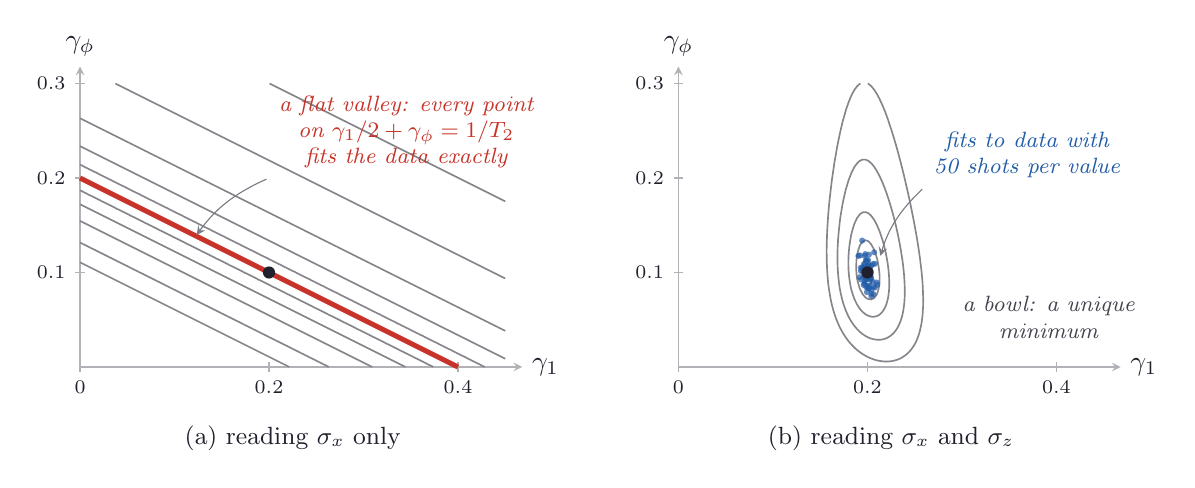
\begin{tikzpicture}[ink/.style={line width=0.9pt, ndInk}, faint/.style={line width=0.4pt, ndInk!35}, dashedink/.style={line width=0.5pt, ndInk!55, dash pattern=on 2.5pt off 2pt}, vec/.style={->, >=stealth, line width=1.2pt}, note/.style={font=\footnotesize\itshape, text=ndInk!85, align=center}, pointer/.style={->, >=stealth, line width=0.4pt, ndInk!60, shorten >=2pt, shorten <=1pt}, dot/.style={circle, fill=ndInk, inner sep=0pt, minimum size=3.4pt}, wash/.style={fill=ndSky, fill opacity=0.55}, every node/.style={text=ndInk}]
\definecolor{ndInk}{rgb}{0.13,0.13,0.18}
\definecolor{ndPaper}{rgb}{0.99,0.96,0.88}
\definecolor{ndSky}{rgb}{0.84,0.91,0.98}
\definecolor{ndRose}{rgb}{0.98,0.86,0.84}
\definecolor{ndBlue}{rgb}{0.13,0.36,0.66}
\definecolor{ndRed}{rgb}{0.78,0.20,0.16}
\definecolor{ndGold}{rgb}{0.88,0.62,0.10}
\definecolor{ndGreen}{rgb}{0.18,0.52,0.30}
\draw[faint, ->, >=stealth] (0.000,0.000) -- (5.616,0.000) node[right, text=ndInk] {$\gamma_1$};
\draw[faint, ->, >=stealth] (0.000,0.000) -- (0.000,3.816) node[above, text=ndInk] {$\gamma_\phi$};
\draw[faint] (0.000,0.060) -- (0.000,-0.060) node[below, font=\scriptsize, text=ndInk] {$0$};
\draw[faint] (2.400,0.060) -- (2.400,-0.060) node[below, font=\scriptsize, text=ndInk] {$0.2$};
\draw[faint] (4.800,0.060) -- (4.800,-0.060) node[below, font=\scriptsize, text=ndInk] {$0.4$};
\draw[faint] (0.060,1.200) -- (-0.060,1.200) node[left, font=\scriptsize, text=ndInk] {$0.1$};
\draw[faint] (0.060,2.400) -- (-0.060,2.400) node[left, font=\scriptsize, text=ndInk] {$0.2$};
\draw[faint] (0.060,3.600) -- (-0.060,3.600) node[left, font=\scriptsize, text=ndInk] {$0.3$};
\draw[line width=0.6pt, ndInk!55] (4.487,0.000) -- (4.464,0.012) -- (4.428,0.029) -- (4.426,0.030) -- (4.392,0.048) -- (4.367,0.060) -- (4.356,0.066) -- (4.320,0.084) -- (4.307,0.090) -- (4.284,0.102) -- (4.248,0.119) -- (4.246,0.120) -- (4.212,0.138) -- (4.187,0.150) -- (4.176,0.156) -- (4.140,0.174) -- (4.127,0.180) -- (4.104,0.192) -- (4.068,0.209) -- (4.066,0.210) -- (4.032,0.228) -- (4.007,0.240) -- (3.996,0.246) -- (3.960,0.264) -- (3.947,0.270) -- (3.924,0.282) -- (3.888,0.299) -- (3.886,0.300) -- (3.852,0.318) -- (3.827,0.330) -- (3.816,0.336) -- (3.780,0.354) -- (3.767,0.360) -- (3.744,0.372) -- (3.708,0.389) -- (3.706,0.390) -- (3.672,0.408) -- (3.647,0.420) -- (3.636,0.426) -- (3.600,0.444) -- (3.587,0.450) -- (3.564,0.462) -- (3.528,0.479) -- (3.526,0.480) -- (3.492,0.498) -- (3.467,0.510) -- (3.456,0.516) -- (3.420,0.534) -- (3.407,0.540) -- (3.384,0.552) -- (3.348,0.569) -- (3.346,0.570) -- (3.312,0.588) -- (3.287,0.600) -- (3.276,0.606) -- (3.240,0.624) -- (3.227,0.630) -- (3.204,0.642) -- (3.168,0.659) -- (3.166,0.660) -- (3.132,0.678) -- (3.107,0.690) -- (3.096,0.696) -- (3.060,0.714) -- (3.047,0.720) -- (3.024,0.732) -- (2.988,0.749) -- (2.986,0.750) -- (2.952,0.768) -- (2.927,0.780) -- (2.916,0.786) -- (2.880,0.804) -- (2.867,0.810) -- (2.844,0.822) -- (2.808,0.839) -- (2.806,0.840) -- (2.772,0.858) -- (2.747,0.870) -- (2.736,0.876) -- (2.700,0.894) -- (2.687,0.900) -- (2.664,0.912) -- (2.628,0.929) -- (2.626,0.930) -- (2.592,0.948) -- (2.567,0.960) -- (2.556,0.966) -- (2.520,0.984) -- (2.507,0.990) -- (2.484,1.002) -- (2.448,1.019) -- (2.446,1.020) -- (2.412,1.038) -- (2.387,1.050) -- (2.376,1.056) -- (2.340,1.074) -- (2.327,1.080) -- (2.304,1.092) -- (2.268,1.109) -- (2.266,1.110) -- (2.232,1.128) -- (2.207,1.140) -- (2.196,1.146) -- (2.160,1.164) -- (2.147,1.170) -- (2.124,1.182) -- (2.088,1.199) -- (2.086,1.200) -- (2.052,1.218) -- (2.027,1.230) -- (2.016,1.236) -- (1.980,1.254) -- (1.967,1.260) -- (1.944,1.272) -- (1.908,1.289) -- (1.906,1.290) -- (1.872,1.308) -- (1.847,1.320) -- (1.836,1.326) -- (1.800,1.344) -- (1.787,1.350) -- (1.764,1.362) -- (1.728,1.379) -- (1.726,1.380) -- (1.692,1.398) -- (1.667,1.410) -- (1.656,1.416) -- (1.620,1.434) -- (1.607,1.440) -- (1.584,1.452) -- (1.548,1.469) -- (1.546,1.470) -- (1.512,1.488) -- (1.487,1.500) -- (1.476,1.506) -- (1.440,1.524) -- (1.427,1.530) -- (1.404,1.542) -- (1.368,1.559) -- (1.366,1.560) -- (1.332,1.578) -- (1.307,1.590) -- (1.296,1.596) -- (1.260,1.614) -- (1.247,1.620) -- (1.224,1.632) -- (1.188,1.649) -- (1.186,1.650) -- (1.152,1.668) -- (1.127,1.680) -- (1.116,1.686) -- (1.080,1.704) -- (1.067,1.710) -- (1.044,1.722) -- (1.008,1.739) -- (1.006,1.740) -- (0.972,1.758) -- (0.947,1.770) -- (0.936,1.776) -- (0.900,1.794) -- (0.887,1.800) -- (0.864,1.812) -- (0.828,1.829) -- (0.826,1.830) -- (0.792,1.848) -- (0.767,1.860) -- (0.756,1.866) -- (0.720,1.884) -- (0.707,1.890) -- (0.684,1.902) -- (0.648,1.919) -- (0.646,1.920) -- (0.612,1.938) -- (0.587,1.950) -- (0.576,1.956) -- (0.540,1.974) -- (0.527,1.980) -- (0.504,1.992) -- (0.468,2.009) -- (0.466,2.010) -- (0.432,2.028) -- (0.407,2.040) -- (0.396,2.046) -- (0.360,2.064) -- (0.347,2.070) -- (0.324,2.082) -- (0.288,2.099) -- (0.286,2.100) -- (0.252,2.118) -- (0.227,2.130) -- (0.216,2.136) -- (0.180,2.154) -- (0.167,2.160) -- (0.144,2.172) -- (0.108,2.189) -- (0.106,2.190) -- (0.072,2.208) -- (0.047,2.220) -- (0.036,2.226) -- (0.000,2.244);
\draw[line width=0.6pt, ndInk!55] (0.000,2.570) -- (0.036,2.553) -- (0.041,2.550) -- (0.072,2.534) -- (0.101,2.520) -- (0.108,2.516) -- (0.144,2.498) -- (0.161,2.490) -- (0.180,2.480) -- (0.216,2.463) -- (0.221,2.460) -- (0.252,2.444) -- (0.281,2.430) -- (0.288,2.426) -- (0.324,2.408) -- (0.341,2.400) -- (0.360,2.390) -- (0.396,2.373) -- (0.401,2.370) -- (0.432,2.354) -- (0.461,2.340) -- (0.468,2.336) -- (0.504,2.318) -- (0.521,2.310) -- (0.540,2.300) -- (0.576,2.283) -- (0.581,2.280) -- (0.612,2.264) -- (0.641,2.250) -- (0.648,2.246) -- (0.684,2.228) -- (0.701,2.220) -- (0.720,2.210) -- (0.756,2.193) -- (0.761,2.190) -- (0.792,2.174) -- (0.821,2.160) -- (0.828,2.156) -- (0.864,2.138) -- (0.881,2.130) -- (0.900,2.120) -- (0.936,2.103) -- (0.941,2.100) -- (0.972,2.084) -- (1.001,2.070) -- (1.008,2.066) -- (1.044,2.048) -- (1.061,2.040) -- (1.080,2.030) -- (1.116,2.013) -- (1.121,2.010) -- (1.152,1.994) -- (1.181,1.980) -- (1.188,1.976) -- (1.224,1.958) -- (1.241,1.950) -- (1.260,1.940) -- (1.296,1.923) -- (1.301,1.920) -- (1.332,1.904) -- (1.361,1.890) -- (1.368,1.886) -- (1.404,1.868) -- (1.421,1.860) -- (1.440,1.850) -- (1.476,1.833) -- (1.481,1.830) -- (1.512,1.814) -- (1.541,1.800) -- (1.548,1.796) -- (1.584,1.778) -- (1.601,1.770) -- (1.620,1.760) -- (1.656,1.743) -- (1.661,1.740) -- (1.692,1.724) -- (1.721,1.710) -- (1.728,1.706) -- (1.764,1.688) -- (1.781,1.680) -- (1.800,1.670) -- (1.836,1.653) -- (1.841,1.650) -- (1.872,1.634) -- (1.901,1.620) -- (1.908,1.616) -- (1.944,1.598) -- (1.961,1.590) -- (1.980,1.580) -- (2.016,1.563) -- (2.021,1.560) -- (2.052,1.544) -- (2.081,1.530) -- (2.088,1.526) -- (2.124,1.508) -- (2.141,1.500) -- (2.160,1.490) -- (2.196,1.473) -- (2.201,1.470) -- (2.232,1.454) -- (2.261,1.440) -- (2.268,1.436) -- (2.304,1.418) -- (2.321,1.410) -- (2.340,1.400) -- (2.376,1.383) -- (2.381,1.380) -- (2.412,1.364) -- (2.441,1.350) -- (2.448,1.346) -- (2.484,1.328) -- (2.501,1.320) -- (2.520,1.310) -- (2.556,1.293) -- (2.561,1.290) -- (2.592,1.274) -- (2.621,1.260) -- (2.628,1.256) -- (2.664,1.238) -- (2.681,1.230) -- (2.700,1.220) -- (2.736,1.203) -- (2.741,1.200) -- (2.772,1.184) -- (2.801,1.170) -- (2.808,1.166) -- (2.844,1.148) -- (2.861,1.140) -- (2.880,1.130) -- (2.916,1.113) -- (2.921,1.110) -- (2.952,1.094) -- (2.981,1.080) -- (2.988,1.076) -- (3.024,1.058) -- (3.041,1.050) -- (3.060,1.040) -- (3.096,1.023) -- (3.101,1.020) -- (3.132,1.004) -- (3.161,0.990) -- (3.168,0.986) -- (3.204,0.968) -- (3.221,0.960) -- (3.240,0.950) -- (3.276,0.933) -- (3.281,0.930) -- (3.312,0.914) -- (3.341,0.900) -- (3.348,0.896) -- (3.384,0.878) -- (3.401,0.870) -- (3.420,0.860) -- (3.456,0.843) -- (3.461,0.840) -- (3.492,0.824) -- (3.521,0.810) -- (3.528,0.806) -- (3.564,0.788) -- (3.581,0.780) -- (3.600,0.770) -- (3.636,0.753) -- (3.641,0.750) -- (3.672,0.734) -- (3.701,0.720) -- (3.708,0.716) -- (3.744,0.698) -- (3.761,0.690) -- (3.780,0.680) -- (3.816,0.663) -- (3.821,0.660) -- (3.852,0.644) -- (3.881,0.630) -- (3.888,0.626) -- (3.924,0.608) -- (3.941,0.600) -- (3.960,0.590) -- (3.996,0.573) -- (4.001,0.570) -- (4.032,0.554) -- (4.061,0.540) -- (4.068,0.536) -- (4.104,0.518) -- (4.121,0.510) -- (4.140,0.500) -- (4.176,0.483) -- (4.181,0.480) -- (4.212,0.464) -- (4.241,0.450) -- (4.248,0.446) -- (4.284,0.428) -- (4.301,0.420) -- (4.320,0.410) -- (4.356,0.393) -- (4.361,0.390) -- (4.392,0.374) -- (4.421,0.360) -- (4.428,0.356) -- (4.464,0.338) -- (4.481,0.330) -- (4.500,0.320) -- (4.536,0.303) -- (4.541,0.300) -- (4.572,0.284) -- (4.601,0.270) -- (4.608,0.266) -- (4.644,0.248) -- (4.661,0.240) -- (4.680,0.230) -- (4.716,0.213) -- (4.721,0.210) -- (4.752,0.194) -- (4.781,0.180) -- (4.788,0.176) -- (4.824,0.158) -- (4.841,0.150) -- (4.860,0.140) -- (4.896,0.123) -- (4.901,0.120) -- (4.932,0.104) -- (4.961,0.090) -- (4.968,0.086) -- (5.004,0.068) -- (5.021,0.060) -- (5.040,0.050) -- (5.076,0.033) -- (5.081,0.030) -- (5.112,0.014) -- (5.141,0.000);
\draw[line width=0.6pt, ndInk!55] (4.132,0.000) -- (4.104,0.014) -- (4.072,0.030) -- (4.068,0.032) -- (4.032,0.050) -- (4.012,0.060) -- (3.996,0.068) -- (3.960,0.086) -- (3.952,0.090) -- (3.924,0.104) -- (3.892,0.120) -- (3.888,0.122) -- (3.852,0.140) -- (3.832,0.150) -- (3.816,0.158) -- (3.780,0.176) -- (3.772,0.180) -- (3.744,0.194) -- (3.712,0.210) -- (3.708,0.212) -- (3.672,0.230) -- (3.652,0.240) -- (3.636,0.248) -- (3.600,0.266) -- (3.592,0.270) -- (3.564,0.284) -- (3.532,0.300) -- (3.528,0.302) -- (3.492,0.320) -- (3.472,0.330) -- (3.456,0.338) -- (3.420,0.356) -- (3.412,0.360) -- (3.384,0.374) -- (3.352,0.390) -- (3.348,0.392) -- (3.312,0.410) -- (3.292,0.420) -- (3.276,0.428) -- (3.240,0.446) -- (3.232,0.450) -- (3.204,0.464) -- (3.172,0.480) -- (3.168,0.482) -- (3.132,0.500) -- (3.112,0.510) -- (3.096,0.518) -- (3.060,0.536) -- (3.052,0.540) -- (3.024,0.554) -- (2.992,0.570) -- (2.988,0.572) -- (2.952,0.590) -- (2.932,0.600) -- (2.916,0.608) -- (2.880,0.626) -- (2.872,0.630) -- (2.844,0.644) -- (2.812,0.660) -- (2.808,0.662) -- (2.772,0.680) -- (2.752,0.690) -- (2.736,0.698) -- (2.700,0.716) -- (2.692,0.720) -- (2.664,0.734) -- (2.632,0.750) -- (2.628,0.752) -- (2.592,0.770) -- (2.572,0.780) -- (2.556,0.788) -- (2.520,0.806) -- (2.512,0.810) -- (2.484,0.824) -- (2.452,0.840) -- (2.448,0.842) -- (2.412,0.860) -- (2.392,0.870) -- (2.376,0.878) -- (2.340,0.896) -- (2.332,0.900) -- (2.304,0.914) -- (2.272,0.930) -- (2.268,0.932) -- (2.232,0.950) -- (2.212,0.960) -- (2.196,0.968) -- (2.160,0.986) -- (2.152,0.990) -- (2.124,1.004) -- (2.092,1.020) -- (2.088,1.022) -- (2.052,1.040) -- (2.032,1.050) -- (2.016,1.058) -- (1.980,1.076) -- (1.972,1.080) -- (1.944,1.094) -- (1.912,1.110) -- (1.908,1.112) -- (1.872,1.130) -- (1.852,1.140) -- (1.836,1.148) -- (1.800,1.166) -- (1.792,1.170) -- (1.764,1.184) -- (1.732,1.200) -- (1.728,1.202) -- (1.692,1.220) -- (1.672,1.230) -- (1.656,1.238) -- (1.620,1.256) -- (1.612,1.260) -- (1.584,1.274) -- (1.552,1.290) -- (1.548,1.292) -- (1.512,1.310) -- (1.492,1.320) -- (1.476,1.328) -- (1.440,1.346) -- (1.432,1.350) -- (1.404,1.364) -- (1.372,1.380) -- (1.368,1.382) -- (1.332,1.400) -- (1.312,1.410) -- (1.296,1.418) -- (1.260,1.436) -- (1.252,1.440) -- (1.224,1.454) -- (1.192,1.470) -- (1.188,1.472) -- (1.152,1.490) -- (1.132,1.500) -- (1.116,1.508) -- (1.080,1.526) -- (1.072,1.530) -- (1.044,1.544) -- (1.012,1.560) -- (1.008,1.562) -- (0.972,1.580) -- (0.952,1.590) -- (0.936,1.598) -- (0.900,1.616) -- (0.892,1.620) -- (0.864,1.634) -- (0.832,1.650) -- (0.828,1.652) -- (0.792,1.670) -- (0.772,1.680) -- (0.756,1.688) -- (0.720,1.706) -- (0.712,1.710) -- (0.684,1.724) -- (0.652,1.740) -- (0.648,1.742) -- (0.612,1.760) -- (0.592,1.770) -- (0.576,1.778) -- (0.540,1.796) -- (0.532,1.800) -- (0.504,1.814) -- (0.472,1.830) -- (0.468,1.832) -- (0.432,1.850) -- (0.412,1.860) -- (0.396,1.868) -- (0.360,1.886) -- (0.352,1.890) -- (0.324,1.904) -- (0.292,1.920) -- (0.288,1.922) -- (0.252,1.940) -- (0.232,1.950) -- (0.216,1.958) -- (0.180,1.976) -- (0.172,1.980) -- (0.144,1.994) -- (0.112,2.010) -- (0.108,2.012) -- (0.072,2.030) -- (0.052,2.040) -- (0.036,2.048) -- (0.000,2.066);
\draw[line width=0.6pt, ndInk!55] (0.000,2.804) -- (0.028,2.790) -- (0.036,2.786) -- (0.072,2.768) -- (0.088,2.760) -- (0.108,2.750) -- (0.144,2.732) -- (0.148,2.730) -- (0.180,2.714) -- (0.208,2.700) -- (0.216,2.696) -- (0.252,2.678) -- (0.268,2.670) -- (0.288,2.660) -- (0.324,2.642) -- (0.328,2.640) -- (0.360,2.624) -- (0.388,2.610) -- (0.396,2.606) -- (0.432,2.588) -- (0.448,2.580) -- (0.468,2.570) -- (0.504,2.552) -- (0.508,2.550) -- (0.540,2.534) -- (0.568,2.520) -- (0.576,2.516) -- (0.612,2.498) -- (0.628,2.490) -- (0.648,2.480) -- (0.684,2.462) -- (0.688,2.460) -- (0.720,2.444) -- (0.748,2.430) -- (0.756,2.426) -- (0.792,2.408) -- (0.808,2.400) -- (0.828,2.390) -- (0.864,2.372) -- (0.868,2.370) -- (0.900,2.354) -- (0.928,2.340) -- (0.936,2.336) -- (0.972,2.318) -- (0.988,2.310) -- (1.008,2.300) -- (1.044,2.282) -- (1.048,2.280) -- (1.080,2.264) -- (1.108,2.250) -- (1.116,2.246) -- (1.152,2.228) -- (1.168,2.220) -- (1.188,2.210) -- (1.224,2.192) -- (1.228,2.190) -- (1.260,2.174) -- (1.288,2.160) -- (1.296,2.156) -- (1.332,2.138) -- (1.348,2.130) -- (1.368,2.120) -- (1.404,2.102) -- (1.408,2.100) -- (1.440,2.084) -- (1.468,2.070) -- (1.476,2.066) -- (1.512,2.048) -- (1.528,2.040) -- (1.548,2.030) -- (1.584,2.012) -- (1.588,2.010) -- (1.620,1.994) -- (1.648,1.980) -- (1.656,1.976) -- (1.692,1.958) -- (1.708,1.950) -- (1.728,1.940) -- (1.764,1.922) -- (1.768,1.920) -- (1.800,1.904) -- (1.828,1.890) -- (1.836,1.886) -- (1.872,1.868) -- (1.888,1.860) -- (1.908,1.850) -- (1.944,1.832) -- (1.948,1.830) -- (1.980,1.814) -- (2.008,1.800) -- (2.016,1.796) -- (2.052,1.778) -- (2.068,1.770) -- (2.088,1.760) -- (2.124,1.742) -- (2.128,1.740) -- (2.160,1.724) -- (2.188,1.710) -- (2.196,1.706) -- (2.232,1.688) -- (2.248,1.680) -- (2.268,1.670) -- (2.304,1.652) -- (2.308,1.650) -- (2.340,1.634) -- (2.368,1.620) -- (2.376,1.616) -- (2.412,1.598) -- (2.428,1.590) -- (2.448,1.580) -- (2.484,1.562) -- (2.488,1.560) -- (2.520,1.544) -- (2.548,1.530) -- (2.556,1.526) -- (2.592,1.508) -- (2.608,1.500) -- (2.628,1.490) -- (2.664,1.472) -- (2.668,1.470) -- (2.700,1.454) -- (2.728,1.440) -- (2.736,1.436) -- (2.772,1.418) -- (2.788,1.410) -- (2.808,1.400) -- (2.844,1.382) -- (2.848,1.380) -- (2.880,1.364) -- (2.908,1.350) -- (2.916,1.346) -- (2.952,1.328) -- (2.968,1.320) -- (2.988,1.310) -- (3.024,1.292) -- (3.028,1.290) -- (3.060,1.274) -- (3.088,1.260) -- (3.096,1.256) -- (3.132,1.238) -- (3.148,1.230) -- (3.168,1.220) -- (3.204,1.202) -- (3.208,1.200) -- (3.240,1.184) -- (3.268,1.170) -- (3.276,1.166) -- (3.312,1.148) -- (3.328,1.140) -- (3.348,1.130) -- (3.384,1.112) -- (3.388,1.110) -- (3.420,1.094) -- (3.448,1.080) -- (3.456,1.076) -- (3.492,1.058) -- (3.508,1.050) -- (3.528,1.040) -- (3.564,1.022) -- (3.568,1.020) -- (3.600,1.004) -- (3.628,0.990) -- (3.636,0.986) -- (3.672,0.968) -- (3.688,0.960) -- (3.708,0.950) -- (3.744,0.932) -- (3.748,0.930) -- (3.780,0.914) -- (3.808,0.900) -- (3.816,0.896) -- (3.852,0.878) -- (3.868,0.870) -- (3.888,0.860) -- (3.924,0.842) -- (3.928,0.840) -- (3.960,0.824) -- (3.988,0.810) -- (3.996,0.806) -- (4.032,0.788) -- (4.048,0.780) -- (4.068,0.770) -- (4.104,0.752) -- (4.108,0.750) -- (4.140,0.734) -- (4.168,0.720) -- (4.176,0.716) -- (4.212,0.698) -- (4.228,0.690) -- (4.248,0.680) -- (4.284,0.662) -- (4.288,0.660) -- (4.320,0.644) -- (4.348,0.630) -- (4.356,0.626) -- (4.392,0.608) -- (4.408,0.600) -- (4.428,0.590) -- (4.464,0.572) -- (4.468,0.570) -- (4.500,0.554) -- (4.528,0.540) -- (4.536,0.536) -- (4.572,0.518) -- (4.588,0.510) -- (4.608,0.500) -- (4.644,0.482) -- (4.648,0.480) -- (4.680,0.464) -- (4.708,0.450) -- (4.716,0.446) -- (4.752,0.428) -- (4.768,0.420) -- (4.788,0.410) -- (4.824,0.392) -- (4.828,0.390) -- (4.860,0.374) -- (4.888,0.360) -- (4.896,0.356) -- (4.932,0.338) -- (4.948,0.330) -- (4.968,0.320) -- (5.004,0.302) -- (5.008,0.300) -- (5.040,0.284) -- (5.068,0.270) -- (5.076,0.266) -- (5.112,0.248) -- (5.128,0.240) -- (5.148,0.230) -- (5.184,0.212) -- (5.188,0.210) -- (5.220,0.194) -- (5.248,0.180) -- (5.256,0.176) -- (5.292,0.158) -- (5.308,0.150) -- (5.328,0.140) -- (5.364,0.122) -- (5.368,0.120) -- (5.400,0.104);
\draw[line width=0.6pt, ndInk!55] (3.710,0.000) -- (3.708,0.001) -- (3.672,0.019) -- (3.650,0.030) -- (3.636,0.037) -- (3.600,0.055) -- (3.590,0.060) -- (3.564,0.073) -- (3.530,0.090) -- (3.528,0.091) -- (3.492,0.109) -- (3.470,0.120) -- (3.456,0.127) -- (3.420,0.145) -- (3.410,0.150) -- (3.384,0.163) -- (3.350,0.180) -- (3.348,0.181) -- (3.312,0.199) -- (3.290,0.210) -- (3.276,0.217) -- (3.240,0.235) -- (3.230,0.240) -- (3.204,0.253) -- (3.170,0.270) -- (3.168,0.271) -- (3.132,0.289) -- (3.110,0.300) -- (3.096,0.307) -- (3.060,0.325) -- (3.050,0.330) -- (3.024,0.343) -- (2.990,0.360) -- (2.988,0.361) -- (2.952,0.379) -- (2.930,0.390) -- (2.916,0.397) -- (2.880,0.415) -- (2.870,0.420) -- (2.844,0.433) -- (2.810,0.450) -- (2.808,0.451) -- (2.772,0.469) -- (2.750,0.480) -- (2.736,0.487) -- (2.700,0.505) -- (2.690,0.510) -- (2.664,0.523) -- (2.630,0.540) -- (2.628,0.541) -- (2.592,0.559) -- (2.570,0.570) -- (2.556,0.577) -- (2.520,0.595) -- (2.510,0.600) -- (2.484,0.613) -- (2.450,0.630) -- (2.448,0.631) -- (2.412,0.649) -- (2.390,0.660) -- (2.376,0.667) -- (2.340,0.685) -- (2.330,0.690) -- (2.304,0.703) -- (2.270,0.720) -- (2.268,0.721) -- (2.232,0.739) -- (2.210,0.750) -- (2.196,0.757) -- (2.160,0.775) -- (2.150,0.780) -- (2.124,0.793) -- (2.090,0.810) -- (2.088,0.811) -- (2.052,0.829) -- (2.030,0.840) -- (2.016,0.847) -- (1.980,0.865) -- (1.970,0.870) -- (1.944,0.883) -- (1.910,0.900) -- (1.908,0.901) -- (1.872,0.919) -- (1.850,0.930) -- (1.836,0.937) -- (1.800,0.955) -- (1.790,0.960) -- (1.764,0.973) -- (1.730,0.990) -- (1.728,0.991) -- (1.692,1.009) -- (1.670,1.020) -- (1.656,1.027) -- (1.620,1.045) -- (1.610,1.050) -- (1.584,1.063) -- (1.550,1.080) -- (1.548,1.081) -- (1.512,1.099) -- (1.490,1.110) -- (1.476,1.117) -- (1.440,1.135) -- (1.430,1.140) -- (1.404,1.153) -- (1.370,1.170) -- (1.368,1.171) -- (1.332,1.189) -- (1.310,1.200) -- (1.296,1.207) -- (1.260,1.225) -- (1.250,1.230) -- (1.224,1.243) -- (1.190,1.260) -- (1.188,1.261) -- (1.152,1.279) -- (1.130,1.290) -- (1.116,1.297) -- (1.080,1.315) -- (1.070,1.320) -- (1.044,1.333) -- (1.010,1.350) -- (1.008,1.351) -- (0.972,1.369) -- (0.950,1.380) -- (0.936,1.387) -- (0.900,1.405) -- (0.890,1.410) -- (0.864,1.423) -- (0.830,1.440) -- (0.828,1.441) -- (0.792,1.459) -- (0.770,1.470) -- (0.756,1.477) -- (0.720,1.495) -- (0.710,1.500) -- (0.684,1.513) -- (0.650,1.530) -- (0.648,1.531) -- (0.612,1.549) -- (0.590,1.560) -- (0.576,1.567) -- (0.540,1.585) -- (0.530,1.590) -- (0.504,1.603) -- (0.470,1.620) -- (0.468,1.621) -- (0.432,1.639) -- (0.410,1.650) -- (0.396,1.657) -- (0.360,1.675) -- (0.350,1.680) -- (0.324,1.693) -- (0.290,1.710) -- (0.288,1.711) -- (0.252,1.729) -- (0.230,1.740) -- (0.216,1.747) -- (0.180,1.765) -- (0.170,1.770) -- (0.144,1.783) -- (0.110,1.800) -- (0.108,1.801) -- (0.072,1.819) -- (0.050,1.830) -- (0.036,1.837) -- (0.000,1.855);
\draw[line width=0.6pt, ndInk!55] (0.000,3.159) -- (0.019,3.150) -- (0.036,3.141) -- (0.072,3.123) -- (0.079,3.120) -- (0.108,3.105) -- (0.139,3.090) -- (0.144,3.087) -- (0.180,3.069) -- (0.199,3.060) -- (0.216,3.051) -- (0.252,3.033) -- (0.259,3.030) -- (0.288,3.015) -- (0.319,3.000) -- (0.324,2.997) -- (0.360,2.979) -- (0.379,2.970) -- (0.396,2.961) -- (0.432,2.943) -- (0.439,2.940) -- (0.468,2.925) -- (0.499,2.910) -- (0.504,2.907) -- (0.540,2.889) -- (0.559,2.880) -- (0.576,2.871) -- (0.612,2.853) -- (0.619,2.850) -- (0.648,2.835) -- (0.679,2.820) -- (0.684,2.817) -- (0.720,2.799) -- (0.739,2.790) -- (0.756,2.781) -- (0.792,2.763) -- (0.799,2.760) -- (0.828,2.745) -- (0.859,2.730) -- (0.864,2.727) -- (0.900,2.709) -- (0.919,2.700) -- (0.936,2.691) -- (0.972,2.673) -- (0.979,2.670) -- (1.008,2.655) -- (1.039,2.640) -- (1.044,2.637) -- (1.080,2.619) -- (1.099,2.610) -- (1.116,2.601) -- (1.152,2.583) -- (1.159,2.580) -- (1.188,2.565) -- (1.219,2.550) -- (1.224,2.547) -- (1.260,2.529) -- (1.279,2.520) -- (1.296,2.511) -- (1.332,2.493) -- (1.339,2.490) -- (1.368,2.475) -- (1.399,2.460) -- (1.404,2.457) -- (1.440,2.439) -- (1.459,2.430) -- (1.476,2.421) -- (1.512,2.403) -- (1.519,2.400) -- (1.548,2.385) -- (1.579,2.370) -- (1.584,2.367) -- (1.620,2.349) -- (1.639,2.340) -- (1.656,2.331) -- (1.692,2.313) -- (1.699,2.310) -- (1.728,2.295) -- (1.759,2.280) -- (1.764,2.277) -- (1.800,2.259) -- (1.819,2.250) -- (1.836,2.241) -- (1.872,2.223) -- (1.879,2.220) -- (1.908,2.205) -- (1.939,2.190) -- (1.944,2.187) -- (1.980,2.169) -- (1.999,2.160) -- (2.016,2.151) -- (2.052,2.133) -- (2.059,2.130) -- (2.088,2.115) -- (2.119,2.100) -- (2.124,2.097) -- (2.160,2.079) -- (2.179,2.070) -- (2.196,2.061) -- (2.232,2.043) -- (2.239,2.040) -- (2.268,2.025) -- (2.299,2.010) -- (2.304,2.007) -- (2.340,1.989) -- (2.359,1.980) -- (2.376,1.971) -- (2.412,1.953) -- (2.419,1.950) -- (2.448,1.935) -- (2.479,1.920) -- (2.484,1.917) -- (2.520,1.899) -- (2.539,1.890) -- (2.556,1.881) -- (2.592,1.863) -- (2.599,1.860) -- (2.628,1.845) -- (2.659,1.830) -- (2.664,1.827) -- (2.700,1.809) -- (2.719,1.800) -- (2.736,1.791) -- (2.772,1.773) -- (2.779,1.770) -- (2.808,1.755) -- (2.839,1.740) -- (2.844,1.737) -- (2.880,1.719) -- (2.899,1.710) -- (2.916,1.701) -- (2.952,1.683) -- (2.959,1.680) -- (2.988,1.665) -- (3.019,1.650) -- (3.024,1.647) -- (3.060,1.629) -- (3.079,1.620) -- (3.096,1.611) -- (3.132,1.593) -- (3.139,1.590) -- (3.168,1.575) -- (3.199,1.560) -- (3.204,1.557) -- (3.240,1.539) -- (3.259,1.530) -- (3.276,1.521) -- (3.312,1.503) -- (3.319,1.500) -- (3.348,1.485) -- (3.379,1.470) -- (3.384,1.467) -- (3.420,1.449) -- (3.439,1.440) -- (3.456,1.431) -- (3.492,1.413) -- (3.499,1.410) -- (3.528,1.395) -- (3.559,1.380) -- (3.564,1.377) -- (3.600,1.359) -- (3.619,1.350) -- (3.636,1.341) -- (3.672,1.323) -- (3.679,1.320) -- (3.708,1.305) -- (3.739,1.290) -- (3.744,1.287) -- (3.780,1.269) -- (3.799,1.260) -- (3.816,1.251) -- (3.852,1.233) -- (3.859,1.230) -- (3.888,1.215) -- (3.919,1.200) -- (3.924,1.197) -- (3.960,1.179) -- (3.979,1.170) -- (3.996,1.161) -- (4.032,1.143) -- (4.039,1.140) -- (4.068,1.125) -- (4.099,1.110) -- (4.104,1.107) -- (4.140,1.089) -- (4.159,1.080) -- (4.176,1.071) -- (4.212,1.053) -- (4.219,1.050) -- (4.248,1.035) -- (4.279,1.020) -- (4.284,1.017) -- (4.320,0.999) -- (4.339,0.990) -- (4.356,0.981) -- (4.392,0.963) -- (4.399,0.960) -- (4.428,0.945) -- (4.459,0.930) -- (4.464,0.927) -- (4.500,0.909) -- (4.519,0.900) -- (4.536,0.891) -- (4.572,0.873) -- (4.579,0.870) -- (4.608,0.855) -- (4.639,0.840) -- (4.644,0.837) -- (4.680,0.819) -- (4.699,0.810) -- (4.716,0.801) -- (4.752,0.783) -- (4.759,0.780) -- (4.788,0.765) -- (4.819,0.750) -- (4.824,0.747) -- (4.860,0.729) -- (4.879,0.720) -- (4.896,0.711) -- (4.932,0.693) -- (4.939,0.690) -- (4.968,0.675) -- (4.999,0.660) -- (5.004,0.657) -- (5.040,0.639) -- (5.059,0.630) -- (5.076,0.621) -- (5.112,0.603) -- (5.119,0.600) -- (5.148,0.585) -- (5.179,0.570) -- (5.184,0.567) -- (5.220,0.549) -- (5.239,0.540) -- (5.256,0.531) -- (5.292,0.513) -- (5.299,0.510) -- (5.328,0.495) -- (5.359,0.480) -- (5.364,0.477) -- (5.400,0.459);
\draw[line width=0.6pt, ndInk!55] (3.160,0.000) -- (3.132,0.014) -- (3.100,0.030) -- (3.096,0.032) -- (3.060,0.050) -- (3.040,0.060) -- (3.024,0.068) -- (2.988,0.086) -- (2.980,0.090) -- (2.952,0.104) -- (2.920,0.120) -- (2.916,0.122) -- (2.880,0.140) -- (2.860,0.150) -- (2.844,0.158) -- (2.808,0.176) -- (2.800,0.180) -- (2.772,0.194) -- (2.740,0.210) -- (2.736,0.212) -- (2.700,0.230) -- (2.680,0.240) -- (2.664,0.248) -- (2.628,0.266) -- (2.620,0.270) -- (2.592,0.284) -- (2.560,0.300) -- (2.556,0.302) -- (2.520,0.320) -- (2.500,0.330) -- (2.484,0.338) -- (2.448,0.356) -- (2.440,0.360) -- (2.412,0.374) -- (2.380,0.390) -- (2.376,0.392) -- (2.340,0.410) -- (2.320,0.420) -- (2.304,0.428) -- (2.268,0.446) -- (2.260,0.450) -- (2.232,0.464) -- (2.200,0.480) -- (2.196,0.482) -- (2.160,0.500) -- (2.140,0.510) -- (2.124,0.518) -- (2.088,0.536) -- (2.080,0.540) -- (2.052,0.554) -- (2.020,0.570) -- (2.016,0.572) -- (1.980,0.590) -- (1.960,0.600) -- (1.944,0.608) -- (1.908,0.626) -- (1.900,0.630) -- (1.872,0.644) -- (1.840,0.660) -- (1.836,0.662) -- (1.800,0.680) -- (1.780,0.690) -- (1.764,0.698) -- (1.728,0.716) -- (1.720,0.720) -- (1.692,0.734) -- (1.660,0.750) -- (1.656,0.752) -- (1.620,0.770) -- (1.600,0.780) -- (1.584,0.788) -- (1.548,0.806) -- (1.540,0.810) -- (1.512,0.824) -- (1.480,0.840) -- (1.476,0.842) -- (1.440,0.860) -- (1.420,0.870) -- (1.404,0.878) -- (1.368,0.896) -- (1.360,0.900) -- (1.332,0.914) -- (1.300,0.930) -- (1.296,0.932) -- (1.260,0.950) -- (1.240,0.960) -- (1.224,0.968) -- (1.188,0.986) -- (1.180,0.990) -- (1.152,1.004) -- (1.120,1.020) -- (1.116,1.022) -- (1.080,1.040) -- (1.060,1.050) -- (1.044,1.058) -- (1.008,1.076) -- (1.000,1.080) -- (0.972,1.094) -- (0.940,1.110) -- (0.936,1.112) -- (0.900,1.130) -- (0.880,1.140) -- (0.864,1.148) -- (0.828,1.166) -- (0.820,1.170) -- (0.792,1.184) -- (0.760,1.200) -- (0.756,1.202) -- (0.720,1.220) -- (0.700,1.230) -- (0.684,1.238) -- (0.648,1.256) -- (0.640,1.260) -- (0.612,1.274) -- (0.580,1.290) -- (0.576,1.292) -- (0.540,1.310) -- (0.520,1.320) -- (0.504,1.328) -- (0.468,1.346) -- (0.460,1.350) -- (0.432,1.364) -- (0.400,1.380) -- (0.396,1.382) -- (0.360,1.400) -- (0.340,1.410) -- (0.324,1.418) -- (0.288,1.436) -- (0.280,1.440) -- (0.252,1.454) -- (0.220,1.470) -- (0.216,1.472) -- (0.180,1.490) -- (0.160,1.500) -- (0.144,1.508) -- (0.108,1.526) -- (0.100,1.530) -- (0.072,1.544) -- (0.040,1.560) -- (0.036,1.562) -- (0.000,1.580);
\draw[line width=0.6pt, ndInk!55] (0.449,3.600) -- (0.468,3.590) -- (0.504,3.572) -- (0.509,3.570) -- (0.540,3.554) -- (0.569,3.540) -- (0.576,3.536) -- (0.612,3.518) -- (0.629,3.510) -- (0.648,3.500) -- (0.684,3.482) -- (0.689,3.480) -- (0.720,3.464) -- (0.749,3.450) -- (0.756,3.446) -- (0.792,3.428) -- (0.809,3.420) -- (0.828,3.410) -- (0.864,3.392) -- (0.869,3.390) -- (0.900,3.374) -- (0.929,3.360) -- (0.936,3.356) -- (0.972,3.338) -- (0.989,3.330) -- (1.008,3.320) -- (1.044,3.302) -- (1.049,3.300) -- (1.080,3.284) -- (1.109,3.270) -- (1.116,3.266) -- (1.152,3.248) -- (1.169,3.240) -- (1.188,3.230) -- (1.224,3.212) -- (1.229,3.210) -- (1.260,3.194) -- (1.289,3.180) -- (1.296,3.176) -- (1.332,3.158) -- (1.349,3.150) -- (1.368,3.140) -- (1.404,3.122) -- (1.409,3.120) -- (1.440,3.104) -- (1.469,3.090) -- (1.476,3.086) -- (1.512,3.068) -- (1.529,3.060) -- (1.548,3.050) -- (1.584,3.032) -- (1.589,3.030) -- (1.620,3.014) -- (1.649,3.000) -- (1.656,2.996) -- (1.692,2.978) -- (1.709,2.970) -- (1.728,2.960) -- (1.764,2.942) -- (1.769,2.940) -- (1.800,2.924) -- (1.829,2.910) -- (1.836,2.906) -- (1.872,2.888) -- (1.889,2.880) -- (1.908,2.870) -- (1.944,2.852) -- (1.949,2.850) -- (1.980,2.834) -- (2.009,2.820) -- (2.016,2.816) -- (2.052,2.798) -- (2.069,2.790) -- (2.088,2.780) -- (2.124,2.762) -- (2.129,2.760) -- (2.160,2.744) -- (2.189,2.730) -- (2.196,2.726) -- (2.232,2.708) -- (2.249,2.700) -- (2.268,2.690) -- (2.304,2.672) -- (2.309,2.670) -- (2.340,2.654) -- (2.369,2.640) -- (2.376,2.636) -- (2.412,2.618) -- (2.429,2.610) -- (2.448,2.600) -- (2.484,2.582) -- (2.489,2.580) -- (2.520,2.564) -- (2.549,2.550) -- (2.556,2.546) -- (2.592,2.528) -- (2.609,2.520) -- (2.628,2.510) -- (2.664,2.492) -- (2.669,2.490) -- (2.700,2.474) -- (2.729,2.460) -- (2.736,2.456) -- (2.772,2.438) -- (2.789,2.430) -- (2.808,2.420) -- (2.844,2.402) -- (2.849,2.400) -- (2.880,2.384) -- (2.909,2.370) -- (2.916,2.366) -- (2.952,2.348) -- (2.969,2.340) -- (2.988,2.330) -- (3.024,2.312) -- (3.029,2.310) -- (3.060,2.294) -- (3.089,2.280) -- (3.096,2.276) -- (3.132,2.258) -- (3.149,2.250) -- (3.168,2.240) -- (3.204,2.222) -- (3.209,2.220) -- (3.240,2.204) -- (3.269,2.190) -- (3.276,2.186) -- (3.312,2.168) -- (3.329,2.160) -- (3.348,2.150) -- (3.384,2.132) -- (3.389,2.130) -- (3.420,2.114) -- (3.449,2.100) -- (3.456,2.096) -- (3.492,2.078) -- (3.509,2.070) -- (3.528,2.060) -- (3.564,2.042) -- (3.569,2.040) -- (3.600,2.024) -- (3.629,2.010) -- (3.636,2.006) -- (3.672,1.988) -- (3.689,1.980) -- (3.708,1.970) -- (3.744,1.952) -- (3.749,1.950) -- (3.780,1.934) -- (3.809,1.920) -- (3.816,1.916) -- (3.852,1.898) -- (3.869,1.890) -- (3.888,1.880) -- (3.924,1.862) -- (3.929,1.860) -- (3.960,1.844) -- (3.989,1.830) -- (3.996,1.826) -- (4.032,1.808) -- (4.049,1.800) -- (4.068,1.790) -- (4.104,1.772) -- (4.109,1.770) -- (4.140,1.754) -- (4.169,1.740) -- (4.176,1.736) -- (4.212,1.718) -- (4.229,1.710) -- (4.248,1.700) -- (4.284,1.682) -- (4.289,1.680) -- (4.320,1.664) -- (4.349,1.650) -- (4.356,1.646) -- (4.392,1.628) -- (4.409,1.620) -- (4.428,1.610) -- (4.464,1.592) -- (4.469,1.590) -- (4.500,1.574) -- (4.529,1.560) -- (4.536,1.556) -- (4.572,1.538) -- (4.589,1.530) -- (4.608,1.520) -- (4.644,1.502) -- (4.649,1.500) -- (4.680,1.484) -- (4.709,1.470) -- (4.716,1.466) -- (4.752,1.448) -- (4.769,1.440) -- (4.788,1.430) -- (4.824,1.412) -- (4.829,1.410) -- (4.860,1.394) -- (4.889,1.380) -- (4.896,1.376) -- (4.932,1.358) -- (4.949,1.350) -- (4.968,1.340) -- (5.004,1.322) -- (5.009,1.320) -- (5.040,1.304) -- (5.069,1.290) -- (5.076,1.286) -- (5.112,1.268) -- (5.129,1.260) -- (5.148,1.250) -- (5.184,1.232) -- (5.189,1.230) -- (5.220,1.214) -- (5.249,1.200) -- (5.256,1.196) -- (5.292,1.178) -- (5.309,1.170) -- (5.328,1.160) -- (5.364,1.142) -- (5.369,1.140) -- (5.400,1.124);
\draw[line width=0.6pt, ndInk!55] (2.658,0.000) -- (2.628,0.015) -- (2.598,0.030) -- (2.592,0.033) -- (2.556,0.051) -- (2.538,0.060) -- (2.520,0.069) -- (2.484,0.087) -- (2.478,0.090) -- (2.448,0.105) -- (2.418,0.120) -- (2.412,0.123) -- (2.376,0.141) -- (2.358,0.150) -- (2.340,0.159) -- (2.304,0.177) -- (2.298,0.180) -- (2.268,0.195) -- (2.238,0.210) -- (2.232,0.213) -- (2.196,0.231) -- (2.178,0.240) -- (2.160,0.249) -- (2.124,0.267) -- (2.118,0.270) -- (2.088,0.285) -- (2.058,0.300) -- (2.052,0.303) -- (2.016,0.321) -- (1.998,0.330) -- (1.980,0.339) -- (1.944,0.357) -- (1.938,0.360) -- (1.908,0.375) -- (1.878,0.390) -- (1.872,0.393) -- (1.836,0.411) -- (1.818,0.420) -- (1.800,0.429) -- (1.764,0.447) -- (1.758,0.450) -- (1.728,0.465) -- (1.698,0.480) -- (1.692,0.483) -- (1.656,0.501) -- (1.638,0.510) -- (1.620,0.519) -- (1.584,0.537) -- (1.578,0.540) -- (1.548,0.555) -- (1.518,0.570) -- (1.512,0.573) -- (1.476,0.591) -- (1.458,0.600) -- (1.440,0.609) -- (1.404,0.627) -- (1.398,0.630) -- (1.368,0.645) -- (1.338,0.660) -- (1.332,0.663) -- (1.296,0.681) -- (1.278,0.690) -- (1.260,0.699) -- (1.224,0.717) -- (1.218,0.720) -- (1.188,0.735) -- (1.158,0.750) -- (1.152,0.753) -- (1.116,0.771) -- (1.098,0.780) -- (1.080,0.789) -- (1.044,0.807) -- (1.038,0.810) -- (1.008,0.825) -- (0.978,0.840) -- (0.972,0.843) -- (0.936,0.861) -- (0.918,0.870) -- (0.900,0.879) -- (0.864,0.897) -- (0.858,0.900) -- (0.828,0.915) -- (0.798,0.930) -- (0.792,0.933) -- (0.756,0.951) -- (0.738,0.960) -- (0.720,0.969) -- (0.684,0.987) -- (0.678,0.990) -- (0.648,1.005) -- (0.618,1.020) -- (0.612,1.023) -- (0.576,1.041) -- (0.558,1.050) -- (0.540,1.059) -- (0.504,1.077) -- (0.498,1.080) -- (0.468,1.095) -- (0.438,1.110) -- (0.432,1.113) -- (0.396,1.131) -- (0.378,1.140) -- (0.360,1.149) -- (0.324,1.167) -- (0.318,1.170) -- (0.288,1.185) -- (0.258,1.200) -- (0.252,1.203) -- (0.216,1.221) -- (0.198,1.230) -- (0.180,1.239) -- (0.144,1.257) -- (0.138,1.260) -- (0.108,1.275) -- (0.078,1.290) -- (0.072,1.293) -- (0.036,1.311) -- (0.018,1.320) -- (0.000,1.329);
\draw[line width=0.6pt, ndInk!55] (2.407,3.600) -- (2.412,3.597) -- (2.448,3.579) -- (2.467,3.570) -- (2.484,3.561) -- (2.520,3.543) -- (2.527,3.540) -- (2.556,3.525) -- (2.587,3.510) -- (2.592,3.507) -- (2.628,3.489) -- (2.647,3.480) -- (2.664,3.471) -- (2.700,3.453) -- (2.707,3.450) -- (2.736,3.435) -- (2.767,3.420) -- (2.772,3.417) -- (2.808,3.399) -- (2.827,3.390) -- (2.844,3.381) -- (2.880,3.363) -- (2.887,3.360) -- (2.916,3.345) -- (2.947,3.330) -- (2.952,3.327) -- (2.988,3.309) -- (3.007,3.300) -- (3.024,3.291) -- (3.060,3.273) -- (3.067,3.270) -- (3.096,3.255) -- (3.127,3.240) -- (3.132,3.237) -- (3.168,3.219) -- (3.187,3.210) -- (3.204,3.201) -- (3.240,3.183) -- (3.247,3.180) -- (3.276,3.165) -- (3.307,3.150) -- (3.312,3.147) -- (3.348,3.129) -- (3.367,3.120) -- (3.384,3.111) -- (3.420,3.093) -- (3.427,3.090) -- (3.456,3.075) -- (3.487,3.060) -- (3.492,3.057) -- (3.528,3.039) -- (3.547,3.030) -- (3.564,3.021) -- (3.600,3.003) -- (3.607,3.000) -- (3.636,2.985) -- (3.667,2.970) -- (3.672,2.967) -- (3.708,2.949) -- (3.727,2.940) -- (3.744,2.931) -- (3.780,2.913) -- (3.787,2.910) -- (3.816,2.895) -- (3.847,2.880) -- (3.852,2.877) -- (3.888,2.859) -- (3.907,2.850) -- (3.924,2.841) -- (3.960,2.823) -- (3.967,2.820) -- (3.996,2.805) -- (4.027,2.790) -- (4.032,2.787) -- (4.068,2.769) -- (4.087,2.760) -- (4.104,2.751) -- (4.140,2.733) -- (4.147,2.730) -- (4.176,2.715) -- (4.207,2.700) -- (4.212,2.697) -- (4.248,2.679) -- (4.267,2.670) -- (4.284,2.661) -- (4.320,2.643) -- (4.327,2.640) -- (4.356,2.625) -- (4.387,2.610) -- (4.392,2.607) -- (4.428,2.589) -- (4.447,2.580) -- (4.464,2.571) -- (4.500,2.553) -- (4.507,2.550) -- (4.536,2.535) -- (4.567,2.520) -- (4.572,2.517) -- (4.608,2.499) -- (4.627,2.490) -- (4.644,2.481) -- (4.680,2.463) -- (4.687,2.460) -- (4.716,2.445) -- (4.747,2.430) -- (4.752,2.427) -- (4.788,2.409) -- (4.807,2.400) -- (4.824,2.391) -- (4.860,2.373) -- (4.867,2.370) -- (4.896,2.355) -- (4.927,2.340) -- (4.932,2.337) -- (4.968,2.319) -- (4.987,2.310) -- (5.004,2.301) -- (5.040,2.283) -- (5.047,2.280) -- (5.076,2.265) -- (5.107,2.250) -- (5.112,2.247) -- (5.148,2.229) -- (5.167,2.220) -- (5.184,2.211) -- (5.220,2.193) -- (5.227,2.190) -- (5.256,2.175) -- (5.287,2.160) -- (5.292,2.157) -- (5.328,2.139) -- (5.347,2.130) -- (5.364,2.121) -- (5.400,2.103);
\draw[line width=1.8pt, ndRed] (0.000,2.400) -- (4.800,0.000);
\node[note, anchor=south west, text=ndRed] (v) at (2.400,2.400) {a flat valley: every point\\ on $\gamma_1/2+\gamma_\phi=1/T_2$\\ fits the data exactly};
\draw[pointer] (v.south west) to[bend right=15] (1.440,1.620);
\node[dot, fill=ndInk, minimum size=4.4pt] at (2.400,1.200) {};
\node[font=\small] at (2.700,-0.900) {(a) reading $\sigma_x$ only};
\draw[faint, ->, >=stealth] (7.600,0.000) -- (13.216,0.000) node[right, text=ndInk] {$\gamma_1$};
\draw[faint, ->, >=stealth] (7.600,0.000) -- (7.600,3.816) node[above, text=ndInk] {$\gamma_\phi$};
\draw[faint] (7.600,0.060) -- (7.600,-0.060) node[below, font=\scriptsize, text=ndInk] {$0$};
\draw[faint] (10.000,0.060) -- (10.000,-0.060) node[below, font=\scriptsize, text=ndInk] {$0.2$};
\draw[faint] (12.400,0.060) -- (12.400,-0.060) node[below, font=\scriptsize, text=ndInk] {$0.4$};
\draw[faint] (7.660,1.200) -- (7.540,1.200) node[left, font=\scriptsize, text=ndInk] {$0.1$};
\draw[faint] (7.660,2.400) -- (7.540,2.400) node[left, font=\scriptsize, text=ndInk] {$0.2$};
\draw[faint] (7.660,3.600) -- (7.540,3.600) node[left, font=\scriptsize, text=ndInk] {$0.3$};
\draw[line width=0.6pt, ndInk!55] (10.019,1.350) -- (10.035,1.320) -- (10.048,1.294) -- (10.049,1.290) -- (10.056,1.260) -- (10.061,1.230) -- (10.064,1.200) -- (10.065,1.170) -- (10.064,1.140) -- (10.061,1.110) -- (10.053,1.080) -- (10.048,1.065) -- (10.029,1.050) -- (10.012,1.040) -- (9.998,1.050) -- (9.976,1.066) -- (9.969,1.080) -- (9.957,1.110) -- (9.947,1.140) -- (9.940,1.165) -- (9.939,1.170) -- (9.937,1.200) -- (9.936,1.230) -- (9.936,1.260) -- (9.939,1.290) -- (9.940,1.297) -- (9.948,1.320) -- (9.962,1.350) -- (9.976,1.370) -- (10.012,1.361) -- (10.019,1.350);
\draw[line width=0.6pt, ndInk!55] (10.018,1.590) -- (10.045,1.560) -- (10.048,1.557) -- (10.063,1.530) -- (10.079,1.500) -- (10.084,1.489) -- (10.091,1.470) -- (10.102,1.440) -- (10.112,1.410) -- (10.120,1.383) -- (10.121,1.380) -- (10.128,1.350) -- (10.134,1.320) -- (10.139,1.290) -- (10.144,1.260) -- (10.148,1.230) -- (10.151,1.200) -- (10.154,1.170) -- (10.155,1.140) -- (10.155,1.110) -- (10.154,1.080) -- (10.151,1.050) -- (10.147,1.020) -- (10.141,0.990) -- (10.133,0.960) -- (10.122,0.930) -- (10.120,0.924) -- (10.104,0.900) -- (10.084,0.875) -- (10.074,0.870) -- (10.048,0.858) -- (10.012,0.861) -- (9.996,0.870) -- (9.976,0.882) -- (9.960,0.900) -- (9.940,0.923) -- (9.936,0.930) -- (9.920,0.960) -- (9.905,0.990) -- (9.904,0.991) -- (9.895,1.020) -- (9.886,1.050) -- (9.878,1.080) -- (9.871,1.110) -- (9.868,1.125) -- (9.866,1.140) -- (9.862,1.170) -- (9.860,1.200) -- (9.858,1.230) -- (9.857,1.260) -- (9.858,1.290) -- (9.859,1.320) -- (9.860,1.350) -- (9.863,1.380) -- (9.867,1.410) -- (9.868,1.418) -- (9.873,1.440) -- (9.880,1.470) -- (9.889,1.500) -- (9.899,1.530) -- (9.904,1.544) -- (9.914,1.560) -- (9.936,1.590) -- (9.940,1.595) -- (9.976,1.610) -- (10.012,1.597) -- (10.018,1.590);
\draw[line width=0.6pt, ndInk!55] (10.015,1.950) -- (10.048,1.920) -- (10.048,1.920) -- (10.070,1.890) -- (10.084,1.870) -- (10.090,1.860) -- (10.106,1.830) -- (10.120,1.804) -- (10.122,1.800) -- (10.134,1.770) -- (10.147,1.740) -- (10.156,1.718) -- (10.159,1.710) -- (10.169,1.680) -- (10.179,1.650) -- (10.189,1.620) -- (10.192,1.611) -- (10.198,1.590) -- (10.206,1.560) -- (10.214,1.530) -- (10.221,1.500) -- (10.228,1.472) -- (10.228,1.470) -- (10.235,1.440) -- (10.240,1.410) -- (10.246,1.380) -- (10.251,1.350) -- (10.256,1.320) -- (10.260,1.290) -- (10.264,1.264) -- (10.264,1.260) -- (10.268,1.230) -- (10.270,1.200) -- (10.273,1.170) -- (10.275,1.140) -- (10.276,1.110) -- (10.277,1.080) -- (10.277,1.050) -- (10.276,1.020) -- (10.275,0.990) -- (10.273,0.960) -- (10.269,0.930) -- (10.266,0.900) -- (10.264,0.891) -- (10.260,0.870) -- (10.253,0.840) -- (10.244,0.810) -- (10.234,0.780) -- (10.228,0.765) -- (10.221,0.750) -- (10.203,0.720) -- (10.192,0.703) -- (10.180,0.690) -- (10.156,0.667) -- (10.146,0.660) -- (10.120,0.646) -- (10.084,0.638) -- (10.048,0.639) -- (10.012,0.650) -- (9.992,0.660) -- (9.976,0.669) -- (9.950,0.690) -- (9.940,0.698) -- (9.920,0.720) -- (9.904,0.739) -- (9.896,0.750) -- (9.877,0.780) -- (9.868,0.794) -- (9.860,0.810) -- (9.845,0.840) -- (9.832,0.869) -- (9.832,0.870) -- (9.821,0.900) -- (9.811,0.930) -- (9.802,0.960) -- (9.796,0.981) -- (9.794,0.990) -- (9.787,1.020) -- (9.782,1.050) -- (9.777,1.080) -- (9.772,1.110) -- (9.768,1.140) -- (9.765,1.170) -- (9.762,1.200) -- (9.760,1.230) -- (9.760,1.231) -- (9.759,1.260) -- (9.758,1.290) -- (9.758,1.320) -- (9.758,1.350) -- (9.759,1.380) -- (9.760,1.410) -- (9.760,1.413) -- (9.762,1.440) -- (9.764,1.470) -- (9.767,1.500) -- (9.770,1.530) -- (9.774,1.560) -- (9.779,1.590) -- (9.784,1.620) -- (9.789,1.650) -- (9.794,1.680) -- (9.796,1.687) -- (9.802,1.710) -- (9.810,1.740) -- (9.819,1.770) -- (9.828,1.800) -- (9.832,1.813) -- (9.839,1.830) -- (9.853,1.860) -- (9.867,1.890) -- (9.868,1.891) -- (9.889,1.920) -- (9.904,1.940) -- (9.919,1.950) -- (9.940,1.964) -- (9.976,1.967) -- (10.012,1.952) -- (10.015,1.950);
\draw[line width=0.6pt, ndInk!55] (10.021,2.610) -- (10.048,2.588) -- (10.055,2.580) -- (10.080,2.550) -- (10.084,2.545) -- (10.100,2.520) -- (10.119,2.490) -- (10.120,2.489) -- (10.135,2.460) -- (10.151,2.430) -- (10.156,2.421) -- (10.165,2.400) -- (10.179,2.370) -- (10.192,2.341) -- (10.192,2.340) -- (10.204,2.310) -- (10.216,2.280) -- (10.227,2.250) -- (10.228,2.249) -- (10.238,2.220) -- (10.248,2.190) -- (10.259,2.160) -- (10.264,2.145) -- (10.269,2.130) -- (10.278,2.100) -- (10.287,2.070) -- (10.296,2.040) -- (10.300,2.028) -- (10.305,2.010) -- (10.313,1.980) -- (10.322,1.950) -- (10.330,1.920) -- (10.336,1.897) -- (10.338,1.890) -- (10.345,1.860) -- (10.352,1.830) -- (10.360,1.800) -- (10.367,1.770) -- (10.372,1.748) -- (10.374,1.740) -- (10.380,1.710) -- (10.387,1.680) -- (10.393,1.650) -- (10.399,1.620) -- (10.405,1.590) -- (10.408,1.575) -- (10.411,1.560) -- (10.416,1.530) -- (10.421,1.500) -- (10.427,1.470) -- (10.431,1.440) -- (10.436,1.410) -- (10.441,1.380) -- (10.444,1.357) -- (10.445,1.350) -- (10.449,1.320) -- (10.453,1.290) -- (10.456,1.260) -- (10.459,1.230) -- (10.462,1.200) -- (10.465,1.170) -- (10.467,1.140) -- (10.469,1.110) -- (10.471,1.080) -- (10.472,1.050) -- (10.473,1.020) -- (10.474,0.990) -- (10.474,0.960) -- (10.474,0.930) -- (10.473,0.900) -- (10.472,0.870) -- (10.470,0.840) -- (10.468,0.810) -- (10.464,0.780) -- (10.460,0.750) -- (10.456,0.720) -- (10.450,0.690) -- (10.444,0.661) -- (10.444,0.660) -- (10.436,0.630) -- (10.426,0.600) -- (10.416,0.570) -- (10.408,0.550) -- (10.403,0.540) -- (10.388,0.510) -- (10.372,0.482) -- (10.371,0.480) -- (10.349,0.450) -- (10.336,0.435) -- (10.321,0.420) -- (10.300,0.401) -- (10.285,0.390) -- (10.264,0.377) -- (10.228,0.360) -- (10.228,0.360) -- (10.192,0.350) -- (10.156,0.345) -- (10.120,0.346) -- (10.084,0.351) -- (10.048,0.360) -- (10.048,0.360) -- (10.012,0.374) -- (9.982,0.390) -- (9.976,0.393) -- (9.940,0.417) -- (9.936,0.420) -- (9.904,0.446) -- (9.900,0.450) -- (9.870,0.480) -- (9.868,0.482) -- (9.844,0.510) -- (9.832,0.525) -- (9.821,0.540) -- (9.800,0.570) -- (9.796,0.576) -- (9.782,0.600) -- (9.765,0.630) -- (9.760,0.640) -- (9.750,0.660) -- (9.737,0.690) -- (9.724,0.719) -- (9.724,0.720) -- (9.713,0.750) -- (9.702,0.780) -- (9.692,0.810) -- (9.688,0.824) -- (9.684,0.840) -- (9.676,0.870) -- (9.669,0.900) -- (9.662,0.930) -- (9.656,0.960) -- (9.652,0.979) -- (9.650,0.990) -- (9.645,1.020) -- (9.641,1.050) -- (9.637,1.080) -- (9.634,1.110) -- (9.631,1.140) -- (9.628,1.170) -- (9.626,1.200) -- (9.624,1.230) -- (9.622,1.260) -- (9.621,1.290) -- (9.620,1.320) -- (9.620,1.350) -- (9.619,1.380) -- (9.619,1.410) -- (9.620,1.440) -- (9.620,1.470) -- (9.621,1.500) -- (9.622,1.530) -- (9.624,1.560) -- (9.626,1.590) -- (9.627,1.620) -- (9.630,1.650) -- (9.632,1.680) -- (9.635,1.710) -- (9.638,1.740) -- (9.641,1.770) -- (9.644,1.800) -- (9.647,1.830) -- (9.651,1.860) -- (9.652,1.870) -- (9.655,1.890) -- (9.659,1.920) -- (9.664,1.950) -- (9.669,1.980) -- (9.674,2.010) -- (9.679,2.040) -- (9.684,2.070) -- (9.688,2.090) -- (9.690,2.100) -- (9.697,2.130) -- (9.703,2.160) -- (9.710,2.190) -- (9.717,2.220) -- (9.724,2.249) -- (9.724,2.250) -- (9.733,2.280) -- (9.742,2.310) -- (9.751,2.340) -- (9.760,2.370) -- (9.760,2.370) -- (9.771,2.400) -- (9.783,2.430) -- (9.794,2.460) -- (9.796,2.465) -- (9.809,2.490) -- (9.824,2.520) -- (9.832,2.536) -- (9.842,2.550) -- (9.864,2.580) -- (9.868,2.586) -- (9.894,2.610) -- (9.904,2.619) -- (9.940,2.634) -- (9.976,2.633) -- (10.012,2.618) -- (10.021,2.610);
\draw[line width=0.6pt, ndInk!55] (10.004,3.600) -- (10.012,3.597) -- (10.044,3.570) -- (10.048,3.567) -- (10.070,3.540) -- (10.084,3.523) -- (10.093,3.510) -- (10.112,3.480) -- (10.120,3.468) -- (10.129,3.450) -- (10.145,3.420) -- (10.156,3.400) -- (10.160,3.390) -- (10.174,3.360) -- (10.188,3.330) -- (10.192,3.321) -- (10.200,3.300) -- (10.213,3.270) -- (10.225,3.240) -- (10.228,3.232) -- (10.236,3.210) -- (10.247,3.180) -- (10.258,3.150) -- (10.264,3.133) -- (10.268,3.120) -- (10.278,3.090) -- (10.288,3.060) -- (10.298,3.030) -- (10.300,3.025) -- (10.308,3.000) -- (10.317,2.970) -- (10.326,2.940) -- (10.336,2.910) -- (10.336,2.909) -- (10.344,2.880) -- (10.353,2.850) -- (10.362,2.820) -- (10.370,2.790) -- (10.372,2.785) -- (10.379,2.760) -- (10.387,2.730) -- (10.395,2.700) -- (10.403,2.670) -- (10.408,2.652) -- (10.411,2.640) -- (10.419,2.610) -- (10.427,2.580) -- (10.434,2.550) -- (10.442,2.520) -- (10.444,2.512) -- (10.449,2.490) -- (10.457,2.460) -- (10.464,2.430) -- (10.471,2.400) -- (10.478,2.370) -- (10.480,2.364) -- (10.485,2.340) -- (10.492,2.310) -- (10.499,2.280) -- (10.506,2.250) -- (10.513,2.220) -- (10.516,2.206) -- (10.520,2.190) -- (10.526,2.160) -- (10.533,2.130) -- (10.539,2.100) -- (10.545,2.070) -- (10.552,2.040) -- (10.552,2.039) -- (10.558,2.010) -- (10.564,1.980) -- (10.570,1.950) -- (10.576,1.920) -- (10.582,1.890) -- (10.588,1.860) -- (10.588,1.859) -- (10.593,1.830) -- (10.599,1.800) -- (10.604,1.770) -- (10.610,1.740) -- (10.615,1.710) -- (10.621,1.680) -- (10.624,1.660) -- (10.626,1.650) -- (10.631,1.620) -- (10.636,1.590) -- (10.640,1.560) -- (10.645,1.530) -- (10.650,1.500) -- (10.654,1.470) -- (10.659,1.440) -- (10.660,1.430) -- (10.663,1.410) -- (10.667,1.380) -- (10.671,1.350) -- (10.674,1.320) -- (10.678,1.290) -- (10.682,1.260) -- (10.685,1.230) -- (10.688,1.200) -- (10.691,1.170) -- (10.694,1.140) -- (10.696,1.113) -- (10.696,1.110) -- (10.699,1.080) -- (10.701,1.050) -- (10.702,1.020) -- (10.704,0.990) -- (10.705,0.960) -- (10.706,0.930) -- (10.707,0.900) -- (10.708,0.870) -- (10.708,0.840) -- (10.707,0.810) -- (10.707,0.780) -- (10.706,0.750) -- (10.704,0.720) -- (10.702,0.690) -- (10.700,0.660) -- (10.697,0.630) -- (10.696,0.623) -- (10.693,0.600) -- (10.689,0.570) -- (10.684,0.540) -- (10.678,0.510) -- (10.671,0.480) -- (10.664,0.450) -- (10.660,0.436) -- (10.655,0.420) -- (10.645,0.390) -- (10.634,0.360) -- (10.624,0.336) -- (10.621,0.330) -- (10.606,0.300) -- (10.589,0.270) -- (10.588,0.268) -- (10.569,0.240) -- (10.552,0.217) -- (10.546,0.210) -- (10.518,0.180) -- (10.516,0.178) -- (10.484,0.150) -- (10.480,0.147) -- (10.444,0.123) -- (10.439,0.120) -- (10.408,0.104) -- (10.372,0.090) -- (10.372,0.090) -- (10.336,0.080) -- (10.300,0.073) -- (10.264,0.070) -- (10.228,0.069) -- (10.192,0.072) -- (10.156,0.077) -- (10.120,0.084) -- (10.100,0.090) -- (10.084,0.095) -- (10.048,0.108) -- (10.019,0.120) -- (10.012,0.123) -- (9.976,0.142) -- (9.962,0.150) -- (9.940,0.163) -- (9.916,0.180) -- (9.904,0.188) -- (9.876,0.210) -- (9.868,0.216) -- (9.841,0.240) -- (9.832,0.249) -- (9.811,0.270) -- (9.796,0.286) -- (9.783,0.300) -- (9.760,0.327) -- (9.758,0.330) -- (9.736,0.360) -- (9.724,0.376) -- (9.715,0.390) -- (9.696,0.420) -- (9.688,0.432) -- (9.678,0.450) -- (9.662,0.480) -- (9.652,0.498) -- (9.646,0.510) -- (9.633,0.540) -- (9.619,0.570) -- (9.616,0.578) -- (9.608,0.600) -- (9.596,0.630) -- (9.586,0.660) -- (9.580,0.677) -- (9.576,0.690) -- (9.567,0.720) -- (9.559,0.750) -- (9.551,0.780) -- (9.544,0.809) -- (9.544,0.810) -- (9.537,0.840) -- (9.531,0.870) -- (9.526,0.900) -- (9.521,0.930) -- (9.516,0.960) -- (9.511,0.990) -- (9.508,1.012) -- (9.507,1.020) -- (9.503,1.050) -- (9.500,1.080) -- (9.497,1.110) -- (9.495,1.140) -- (9.492,1.170) -- (9.490,1.200) -- (9.488,1.230) -- (9.487,1.260) -- (9.486,1.290) -- (9.484,1.320) -- (9.484,1.350) -- (9.483,1.380) -- (9.483,1.410) -- (9.482,1.440) -- (9.482,1.470) -- (9.482,1.500) -- (9.483,1.530) -- (9.483,1.560) -- (9.484,1.590) -- (9.485,1.620) -- (9.486,1.650) -- (9.487,1.680) -- (9.488,1.710) -- (9.490,1.740) -- (9.491,1.770) -- (9.493,1.800) -- (9.495,1.830) -- (9.497,1.860) -- (9.499,1.890) -- (9.501,1.920) -- (9.503,1.950) -- (9.506,1.980) -- (9.508,2.006) -- (9.508,2.010) -- (9.511,2.040) -- (9.514,2.070) -- (9.517,2.100) -- (9.520,2.130) -- (9.523,2.160) -- (9.527,2.190) -- (9.530,2.220) -- (9.534,2.250) -- (9.537,2.280) -- (9.541,2.310) -- (9.544,2.339) -- (9.544,2.340) -- (9.548,2.370) -- (9.552,2.400) -- (9.557,2.430) -- (9.561,2.460) -- (9.565,2.490) -- (9.570,2.520) -- (9.574,2.550) -- (9.578,2.580) -- (9.580,2.591) -- (9.583,2.610) -- (9.588,2.640) -- (9.594,2.670) -- (9.599,2.700) -- (9.604,2.730) -- (9.609,2.760) -- (9.614,2.790) -- (9.616,2.799) -- (9.620,2.820) -- (9.626,2.850) -- (9.632,2.880) -- (9.639,2.910) -- (9.645,2.940) -- (9.651,2.970) -- (9.652,2.976) -- (9.658,3.000) -- (9.665,3.030) -- (9.672,3.060) -- (9.679,3.090) -- (9.686,3.120) -- (9.688,3.127) -- (9.695,3.150) -- (9.703,3.180) -- (9.712,3.210) -- (9.720,3.240) -- (9.724,3.254) -- (9.729,3.270) -- (9.739,3.300) -- (9.750,3.330) -- (9.760,3.360) -- (9.760,3.361) -- (9.772,3.390) -- (9.784,3.420) -- (9.796,3.448) -- (9.797,3.450) -- (9.813,3.480) -- (9.829,3.510) -- (9.832,3.515) -- (9.850,3.540) -- (9.868,3.565) -- (9.874,3.570) -- (9.904,3.597) -- (9.911,3.600);
\fill[ndBlue, opacity=0.7] (9.933,1.605) circle (1.1pt);
\fill[ndBlue, opacity=0.7] (9.999,1.287) circle (1.1pt);
\fill[ndBlue, opacity=0.7] (10.003,1.117) circle (1.1pt);
\fill[ndBlue, opacity=0.7] (9.961,1.058) circle (1.1pt);
\fill[ndBlue, opacity=0.7] (10.012,0.996) circle (1.1pt);
\fill[ndBlue, opacity=0.7] (9.987,1.179) circle (1.1pt);
\fill[ndBlue, opacity=0.7] (9.985,1.014) circle (1.1pt);
\fill[ndBlue, opacity=0.7] (10.006,1.287) circle (1.1pt);
\fill[ndBlue, opacity=0.7] (9.974,1.434) circle (1.1pt);
\fill[ndBlue, opacity=0.7] (10.037,1.110) circle (1.1pt);
\fill[ndBlue, opacity=0.7] (10.022,1.035) circle (1.1pt);
\fill[ndBlue, opacity=0.7] (9.987,1.338) circle (1.1pt);
\fill[ndBlue, opacity=0.7] (10.019,1.427) circle (1.1pt);
\fill[ndBlue, opacity=0.7] (9.989,1.126) circle (1.1pt);
\fill[ndBlue, opacity=0.7] (10.025,1.173) circle (1.1pt);
\fill[ndBlue, opacity=0.7] (9.965,1.411) circle (1.1pt);
\fill[ndBlue, opacity=0.7] (10.023,1.001) circle (1.1pt);
\fill[ndBlue, opacity=0.7] (9.937,1.254) circle (1.1pt);
\fill[ndBlue, opacity=0.7] (10.002,1.019) circle (1.1pt);
\fill[ndBlue, opacity=0.7] (9.995,1.260) circle (1.1pt);
\fill[ndBlue, opacity=0.7] (10.125,1.045) circle (1.1pt);
\fill[ndBlue, opacity=0.7] (10.048,1.287) circle (1.1pt);
\fill[ndBlue, opacity=0.7] (9.903,1.141) circle (1.1pt);
\fill[ndBlue, opacity=0.7] (9.918,1.112) circle (1.1pt);
\fill[ndBlue, opacity=0.7] (10.078,1.016) circle (1.1pt);
\fill[ndBlue, opacity=0.7] (9.885,1.411) circle (1.1pt);
\fill[ndBlue, opacity=0.7] (10.051,0.981) circle (1.1pt);
\fill[ndBlue, opacity=0.7] (10.064,1.085) circle (1.1pt);
\fill[ndBlue, opacity=0.7] (10.017,1.266) circle (1.1pt);
\fill[ndBlue, opacity=0.7] (10.116,1.073) circle (1.1pt);
\fill[ndBlue, opacity=0.7] (10.004,1.227) circle (1.1pt);
\fill[ndBlue, opacity=0.7] (9.993,0.950) circle (1.1pt);
\fill[ndBlue, opacity=0.7] (10.008,1.359) circle (1.1pt);
\fill[ndBlue, opacity=0.7] (9.969,1.229) circle (1.1pt);
\fill[ndBlue, opacity=0.7] (9.987,1.123) circle (1.1pt);
\fill[ndBlue, opacity=0.7] (9.958,1.275) circle (1.1pt);
\fill[ndBlue, opacity=0.7] (10.041,1.217) circle (1.1pt);
\fill[ndBlue, opacity=0.7] (10.085,1.457) circle (1.1pt);
\fill[ndBlue, opacity=0.7] (9.952,1.042) circle (1.1pt);
\fill[ndBlue, opacity=0.7] (9.957,1.309) circle (1.1pt);
\fill[ndBlue, opacity=0.7] (9.936,1.226) circle (1.1pt);
\fill[ndBlue, opacity=0.7] (10.046,1.130) circle (1.1pt);
\fill[ndBlue, opacity=0.7] (9.982,1.357) circle (1.1pt);
\fill[ndBlue, opacity=0.7] (9.966,1.085) circle (1.1pt);
\fill[ndBlue, opacity=0.7] (10.095,1.009) circle (1.1pt);
\fill[ndBlue, opacity=0.7] (9.985,1.229) circle (1.1pt);
\fill[ndBlue, opacity=0.7] (10.096,1.311) circle (1.1pt);
\fill[ndBlue, opacity=0.7] (10.011,1.253) circle (1.1pt);
\fill[ndBlue, opacity=0.7] (10.049,0.900) circle (1.1pt);
\fill[ndBlue, opacity=0.7] (9.978,1.158) circle (1.1pt);
\fill[ndBlue, opacity=0.7] (10.078,0.924) circle (1.1pt);
\fill[ndBlue, opacity=0.7] (9.955,1.151) circle (1.1pt);
\fill[ndBlue, opacity=0.7] (9.994,1.247) circle (1.1pt);
\fill[ndBlue, opacity=0.7] (9.917,1.218) circle (1.1pt);
\fill[ndBlue, opacity=0.7] (10.070,1.307) circle (1.1pt);
\fill[ndBlue, opacity=0.7] (10.037,1.140) circle (1.1pt);
\fill[ndBlue, opacity=0.7] (9.915,1.261) circle (1.1pt);
\fill[ndBlue, opacity=0.7] (9.904,1.417) circle (1.1pt);
\fill[ndBlue, opacity=0.7] (10.051,0.930) circle (1.1pt);
\fill[ndBlue, opacity=0.7] (9.935,1.256) circle (1.1pt);
\node[note, anchor=south west, text=ndBlue] (f) at (10.720,2.280) {fits to data with\\ 50 shots per value};
\draw[pointer] (f.south west) to[bend right=15] (10.144,1.344);
\node[note, anchor=north west] at (11.080,1.020) {a bowl: a unique\\ minimum};
\node[dot, fill=ndInk, minimum size=4.4pt] at (10.000,1.200) {};
\node[font=\small] at (10.300,-0.900) {(b) reading $\sigma_x$ and $\sigma_z$};
\end{tikzpicture}
}\end{center}
$\sigma_x$ only: the rates enter only as $1/T_2=\gamma_1/2+\gamma_\phi$, a \alert{flat valley}. Adding $\sigma_z$: a bowl.}
\end{frame}

\begin{frame}\ft{Three different properties}
\ona{The three properties are logically independent, as Figure~\ref{fig:ch04:distinct} shows for six experiments, with every entry computed. Preparing only $\ket1$ makes the system uncontrollable, although the readout sees everything: the transverse components are never excited, so $\omega$ and $\gamma_\phi$ never leave a trace in the data. Reading only $\sigma_z$ makes it unobservable, although every state can be prepared, with the same consequence. Reading only $\sigma_x$ gives the valley of Figure~\ref{fig:ch04:valley}, and reading $\sigma_x$ and $\sigma_z$ identifies everything. Even a controllable and observable system need not be identifiable. If neither the preparation nor the readout is known, the data determine $\mathbf A$ only up to a similarity, a $16$-dimensional ambiguity for the embedded qubit, which is known in quantum characterisation as the gauge freedom of gate-set tomography. And for two qubits read out completely, an arbitrary Kossakowski matrix cannot be recovered, since $\mathbf R_2$ is rank-deficient, although one supported where the physical one is can. Identifiability therefore needs controllability and observability of the part of the system on which the parameters act, and, in addition, a fixed frame and an injective map from the parameters to the matrices.}
\ona{\begin{figure}[H]\centering
\resizebox{\linewidth}{!}{% Generated by code/needham.py -- do not edit by hand.
\definecolor{qocA}{rgb}{0.00,0.45,0.70}
\definecolor{qocB}{rgb}{0.90,0.60,0.00}
\definecolor{qocC}{rgb}{0.00,0.62,0.45}
\definecolor{qocD}{rgb}{0.80,0.40,0.00}
\definecolor{qocE}{rgb}{0.80,0.60,0.70}
\definecolor{qocF}{rgb}{0.35,0.70,0.90}
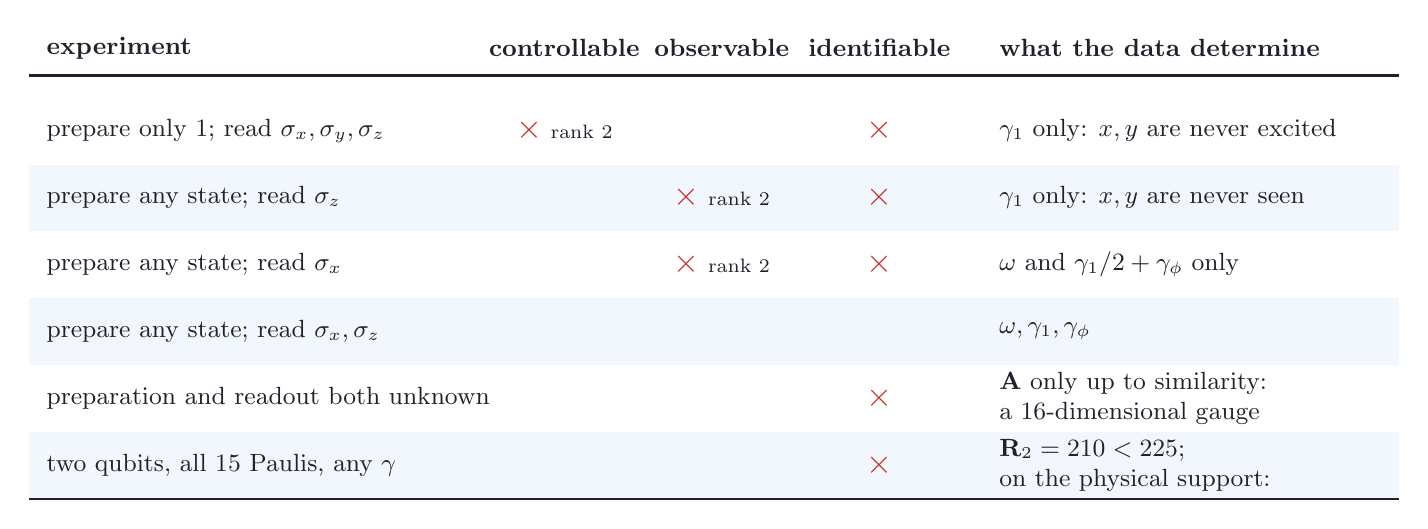
\begin{tikzpicture}[ink/.style={line width=0.9pt, ndInk}, faint/.style={line width=0.4pt, ndInk!35}, dashedink/.style={line width=0.5pt, ndInk!55, dash pattern=on 2.5pt off 2pt}, vec/.style={->, >=stealth, line width=1.2pt}, note/.style={font=\footnotesize\itshape, text=ndInk!85, align=center}, pointer/.style={->, >=stealth, line width=0.4pt, ndInk!60, shorten >=2pt, shorten <=1pt}, dot/.style={circle, fill=ndInk, inner sep=0pt, minimum size=3.4pt}, wash/.style={fill=ndSky, fill opacity=0.55}, every node/.style={text=ndInk}]
\definecolor{ndInk}{rgb}{0.13,0.13,0.18}
\definecolor{ndPaper}{rgb}{0.99,0.96,0.88}
\definecolor{ndSky}{rgb}{0.84,0.91,0.98}
\definecolor{ndRose}{rgb}{0.98,0.86,0.84}
\definecolor{ndBlue}{rgb}{0.13,0.36,0.66}
\definecolor{ndRed}{rgb}{0.78,0.20,0.16}
\definecolor{ndGold}{rgb}{0.88,0.62,0.10}
\definecolor{ndGreen}{rgb}{0.18,0.52,0.30}
\node[anchor=west, font=\small\bfseries] at (0.00,0.6) {experiment};
\node[anchor=center, font=\small\bfseries] at (6.70,0.6) {controllable};
\node[anchor=center, font=\small\bfseries] at (8.70,0.6) {observable};
\node[anchor=center, font=\small\bfseries] at (10.70,0.6) {identifiable};
\node[anchor=west, font=\small\bfseries] at (12.10,0.6) {what the data determine};
\draw[ink] (-0.1,0.25) -- (17.3,0.25);
\node[anchor=west, font=\small] at (0.0,-0.45) {prepare only $\ket1$; read $\sigma_x,\sigma_y,\sigma_z$};
\node[font=\small] at (6.70,-0.45) {\textcolor{ndRed}{\large $\times$}\ {\scriptsize rank $2$}};
\node[font=\small] at (8.70,-0.45) {\textcolor{ndGreen}{\large $\checkmark$}};
\node[font=\small] at (10.70,-0.45) {\textcolor{ndRed}{\large $\times$}};
\node[anchor=west, font=\small, align=left] at (12.1,-0.45) {$\gamma_1$ only: $x,y$ are never excited};
\fill[ndSky, opacity=0.35] (-0.1,-0.88) rectangle (17.3,-1.73);
\node[anchor=west, font=\small] at (0.0,-1.30) {prepare any state; read $\sigma_z$};
\node[font=\small] at (6.70,-1.30) {\textcolor{ndGreen}{\large $\checkmark$}};
\node[font=\small] at (8.70,-1.30) {\textcolor{ndRed}{\large $\times$}\ {\scriptsize rank $2$}};
\node[font=\small] at (10.70,-1.30) {\textcolor{ndRed}{\large $\times$}};
\node[anchor=west, font=\small, align=left] at (12.1,-1.30) {$\gamma_1$ only: $x,y$ are never seen};
\node[anchor=west, font=\small] at (0.0,-2.15) {prepare any state; read $\sigma_x$};
\node[font=\small] at (6.70,-2.15) {\textcolor{ndGreen}{\large $\checkmark$}};
\node[font=\small] at (8.70,-2.15) {\textcolor{ndRed}{\large $\times$}\ {\scriptsize rank $2$}};
\node[font=\small] at (10.70,-2.15) {\textcolor{ndRed}{\large $\times$}};
\node[anchor=west, font=\small, align=left] at (12.1,-2.15) {$\omega$ and $\gamma_1/2+\gamma_\phi$ only};
\fill[ndSky, opacity=0.35] (-0.1,-2.58) rectangle (17.3,-3.43);
\node[anchor=west, font=\small] at (0.0,-3.00) {prepare any state; read $\sigma_x,\sigma_z$};
\node[font=\small] at (6.70,-3.00) {\textcolor{ndGreen}{\large $\checkmark$}};
\node[font=\small] at (8.70,-3.00) {\textcolor{ndGreen}{\large $\checkmark$}};
\node[font=\small] at (10.70,-3.00) {\textcolor{ndGreen}{\large $\checkmark$}};
\node[anchor=west, font=\small, align=left] at (12.1,-3.00) {$\omega,\gamma_1,\gamma_\phi$};
\node[anchor=west, font=\small] at (0.0,-3.85) {preparation and readout both unknown};
\node[font=\small] at (6.70,-3.85) {\textcolor{ndGreen}{\large $\checkmark$}};
\node[font=\small] at (8.70,-3.85) {\textcolor{ndGreen}{\large $\checkmark$}};
\node[font=\small] at (10.70,-3.85) {\textcolor{ndRed}{\large $\times$}};
\node[anchor=west, font=\small, align=left] at (12.1,-3.85) {$\mathbf A$ only up to similarity:\\ a $16$-dimensional gauge};
\fill[ndSky, opacity=0.35] (-0.1,-4.28) rectangle (17.3,-5.13);
\node[anchor=west, font=\small] at (0.0,-4.70) {two qubits, all $15$ Paulis, any $\gamma$};
\node[font=\small] at (6.70,-4.70) {\textcolor{ndGreen}{\large $\checkmark$}};
\node[font=\small] at (8.70,-4.70) {\textcolor{ndGreen}{\large $\checkmark$}};
\node[font=\small] at (10.70,-4.70) {\textcolor{ndRed}{\large $\times$}};
\node[anchor=west, font=\small, align=left] at (12.1,-4.70) {$\rank\mathbf R_2=210<225$;\\ on the physical support: \textcolor{ndGreen}{$\checkmark$}};
\draw[ink] (-0.1,-5.13) -- (17.3,-5.13);
\end{tikzpicture}
}
\caption{Controllability, observability and identifiability in six experiments, all computed: the rank of $[\mathbf B,\mathbf A\mathbf B,\mathbf A^2\mathbf B,\mathbf A^3\mathbf B]$ for the prepared states and of $\OM$ for the readout of the embedded qubit, and the rank of the Jacobian of the sampled outputs with respect to $(\omega,\gamma_1,\gamma_\phi)$; for the black box, the dimension of the similarity ambiguity; for two qubits, the rank of $\mathbf R_2$ (Section~\ref{sec:ch04:example}). Generated by \texttt{code/ch04\_distinct.py}.}\label{fig:ch04:distinct}
\end{figure}}
\onp{\begin{center}\resizebox{\linewidth}{!}{% Generated by code/needham.py -- do not edit by hand.
\definecolor{qocA}{rgb}{0.00,0.45,0.70}
\definecolor{qocB}{rgb}{0.90,0.60,0.00}
\definecolor{qocC}{rgb}{0.00,0.62,0.45}
\definecolor{qocD}{rgb}{0.80,0.40,0.00}
\definecolor{qocE}{rgb}{0.80,0.60,0.70}
\definecolor{qocF}{rgb}{0.35,0.70,0.90}
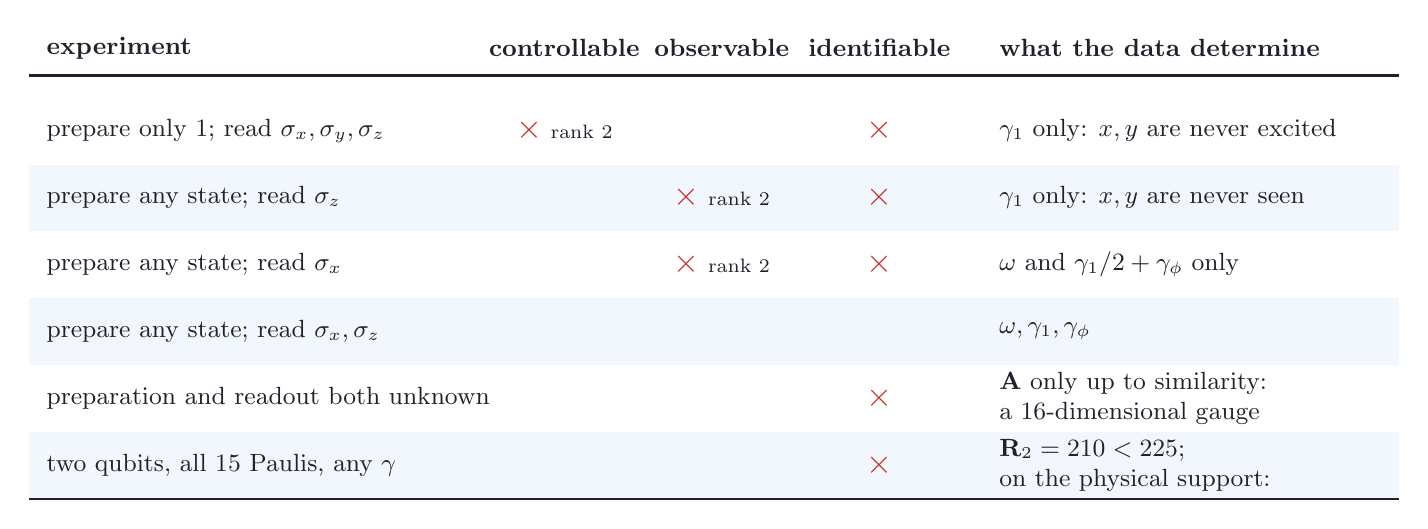
\begin{tikzpicture}[ink/.style={line width=0.9pt, ndInk}, faint/.style={line width=0.4pt, ndInk!35}, dashedink/.style={line width=0.5pt, ndInk!55, dash pattern=on 2.5pt off 2pt}, vec/.style={->, >=stealth, line width=1.2pt}, note/.style={font=\footnotesize\itshape, text=ndInk!85, align=center}, pointer/.style={->, >=stealth, line width=0.4pt, ndInk!60, shorten >=2pt, shorten <=1pt}, dot/.style={circle, fill=ndInk, inner sep=0pt, minimum size=3.4pt}, wash/.style={fill=ndSky, fill opacity=0.55}, every node/.style={text=ndInk}]
\definecolor{ndInk}{rgb}{0.13,0.13,0.18}
\definecolor{ndPaper}{rgb}{0.99,0.96,0.88}
\definecolor{ndSky}{rgb}{0.84,0.91,0.98}
\definecolor{ndRose}{rgb}{0.98,0.86,0.84}
\definecolor{ndBlue}{rgb}{0.13,0.36,0.66}
\definecolor{ndRed}{rgb}{0.78,0.20,0.16}
\definecolor{ndGold}{rgb}{0.88,0.62,0.10}
\definecolor{ndGreen}{rgb}{0.18,0.52,0.30}
\node[anchor=west, font=\small\bfseries] at (0.00,0.6) {experiment};
\node[anchor=center, font=\small\bfseries] at (6.70,0.6) {controllable};
\node[anchor=center, font=\small\bfseries] at (8.70,0.6) {observable};
\node[anchor=center, font=\small\bfseries] at (10.70,0.6) {identifiable};
\node[anchor=west, font=\small\bfseries] at (12.10,0.6) {what the data determine};
\draw[ink] (-0.1,0.25) -- (17.3,0.25);
\node[anchor=west, font=\small] at (0.0,-0.45) {prepare only $\ket1$; read $\sigma_x,\sigma_y,\sigma_z$};
\node[font=\small] at (6.70,-0.45) {\textcolor{ndRed}{\large $\times$}\ {\scriptsize rank $2$}};
\node[font=\small] at (8.70,-0.45) {\textcolor{ndGreen}{\large $\checkmark$}};
\node[font=\small] at (10.70,-0.45) {\textcolor{ndRed}{\large $\times$}};
\node[anchor=west, font=\small, align=left] at (12.1,-0.45) {$\gamma_1$ only: $x,y$ are never excited};
\fill[ndSky, opacity=0.35] (-0.1,-0.88) rectangle (17.3,-1.73);
\node[anchor=west, font=\small] at (0.0,-1.30) {prepare any state; read $\sigma_z$};
\node[font=\small] at (6.70,-1.30) {\textcolor{ndGreen}{\large $\checkmark$}};
\node[font=\small] at (8.70,-1.30) {\textcolor{ndRed}{\large $\times$}\ {\scriptsize rank $2$}};
\node[font=\small] at (10.70,-1.30) {\textcolor{ndRed}{\large $\times$}};
\node[anchor=west, font=\small, align=left] at (12.1,-1.30) {$\gamma_1$ only: $x,y$ are never seen};
\node[anchor=west, font=\small] at (0.0,-2.15) {prepare any state; read $\sigma_x$};
\node[font=\small] at (6.70,-2.15) {\textcolor{ndGreen}{\large $\checkmark$}};
\node[font=\small] at (8.70,-2.15) {\textcolor{ndRed}{\large $\times$}\ {\scriptsize rank $2$}};
\node[font=\small] at (10.70,-2.15) {\textcolor{ndRed}{\large $\times$}};
\node[anchor=west, font=\small, align=left] at (12.1,-2.15) {$\omega$ and $\gamma_1/2+\gamma_\phi$ only};
\fill[ndSky, opacity=0.35] (-0.1,-2.58) rectangle (17.3,-3.43);
\node[anchor=west, font=\small] at (0.0,-3.00) {prepare any state; read $\sigma_x,\sigma_z$};
\node[font=\small] at (6.70,-3.00) {\textcolor{ndGreen}{\large $\checkmark$}};
\node[font=\small] at (8.70,-3.00) {\textcolor{ndGreen}{\large $\checkmark$}};
\node[font=\small] at (10.70,-3.00) {\textcolor{ndGreen}{\large $\checkmark$}};
\node[anchor=west, font=\small, align=left] at (12.1,-3.00) {$\omega,\gamma_1,\gamma_\phi$};
\node[anchor=west, font=\small] at (0.0,-3.85) {preparation and readout both unknown};
\node[font=\small] at (6.70,-3.85) {\textcolor{ndGreen}{\large $\checkmark$}};
\node[font=\small] at (8.70,-3.85) {\textcolor{ndGreen}{\large $\checkmark$}};
\node[font=\small] at (10.70,-3.85) {\textcolor{ndRed}{\large $\times$}};
\node[anchor=west, font=\small, align=left] at (12.1,-3.85) {$\mathbf A$ only up to similarity:\\ a $16$-dimensional gauge};
\fill[ndSky, opacity=0.35] (-0.1,-4.28) rectangle (17.3,-5.13);
\node[anchor=west, font=\small] at (0.0,-4.70) {two qubits, all $15$ Paulis, any $\gamma$};
\node[font=\small] at (6.70,-4.70) {\textcolor{ndGreen}{\large $\checkmark$}};
\node[font=\small] at (8.70,-4.70) {\textcolor{ndGreen}{\large $\checkmark$}};
\node[font=\small] at (10.70,-4.70) {\textcolor{ndRed}{\large $\times$}};
\node[anchor=west, font=\small, align=left] at (12.1,-4.70) {$\rank\mathbf R_2=210<225$;\\ on the physical support: \textcolor{ndGreen}{$\checkmark$}};
\draw[ink] (-0.1,-5.13) -- (17.3,-5.13);
\end{tikzpicture}
}\end{center}
Three different questions: each can fail while the others hold.}
\end{frame}

\begin{frame}\ft{From the system matrix back to the master equation}\mop{\footnotesize}
\ona{Assume the system matrix is known as the result of some identification procedure (\Chap~\ref{C.AlgTomography}). The system matrix is of the form $\mathbf{A}(\vec\theta,\Koss) = \mathbf{A}^{(l)}(\vec{\theta}) + \mathbf{A}^{(d)}(\Koss)$, linear in $\vec\theta$ and in $\Koss$. To discuss the recovery of the parameters of the original GKSL equation, consider the map $\phi:\R^{n}\times\Herm[n]\rightarrow\R^{n\times n}$, $\phi(\vec{\theta},\Koss)=\mathbf{A}^{(l)}(\vec{\theta})+\mathbf{A}^{(d)}(\Koss)$, and the map $\hat{\phi}:\Herm[n]\rightarrow\R^{n}$ producing $\vec\beta$, $\hat{\phi}(\Koss)=\big(\frac{\imath}{N}\sum_{k,l=1}^{n}\gamma_{kl}f_{jkl}\big)_{j=1}^{n}$. We are interested in the conditions under which $\phi$ and $\hat{\phi}$ can be inverted, which amounts to the unique reconstruction of $\vec{\theta}$ and $\Koss$ from known values of $\mathbf{A}$ and $\vec{\beta}$. Let $\Gamma :  \{1, \dots , n^{2} \} \rightarrow  \{  (j,k) : j,k \in \{1, \dots, n\}  \}$ be a bijective indexing used to vectorise $\mathbf{A}^{(l)}, \mathbf{A}^{(d)}$ and $\Koss$, and define}
\onp{$\mathbf A=\mathbf A^{(l)}(\vec\theta)+\mathbf A^{(d)}(\Koss)$ is \alert{linear} in the unknowns. Vectorise with an index map $\Gamma:\{1,\dots,n^2\}\to\{(j,k)\}$:}
\begin{equation}\label{eq:ch04:T1T2}
\mathbf{R}_{1}= - \begin{pmatrix}f_{\Gamma(1)1} & \cdots & f_{\Gamma(1)n}\\
\vdots & \ddots & \vdots\\
f_{\Gamma(n^{2})1} & \cdots & f_{\Gamma(n^{2})n}
\end{pmatrix} \in \R^{n^2 \times n}, \qquad
\mathbf{R}_{2}= -\begin{pmatrix}D_{\Gamma(1)}^{(\Gamma(1))} & \cdots & D_{\Gamma(n^{2})}^{(\Gamma(1))} \\
\vdots & \ddots & \vdots\\
D_{\Gamma(1)}^{(\Gamma(n^{2}))} & \cdots & D_{\Gamma(n^{2})}^{(\Gamma(n^{2}))}
\end{pmatrix}\in \C^{n^2 \times n^2},
\end{equation}
\ona{where $D^{(j,k)}_{lm}$ is the dissipation tensor of \Chap~\ref{C.Open}, so that $\vecop{\mathbf A^{(l)}}=\mathbf R_1\vec\theta$ and $\vecop{\mathbf A^{(d)}}=\mathbf R_2\vecop{\Koss}$. Furthermore, define}
\begin{equation}\label{eq:ch04:M}
\mathbf{M}=\left[\begin{array}{cc}
\mathbf{R}_{1} & \mathbf{R}_{2}\\
0 & -\frac{\imath}{N}\mathbf{R}_1^{\top}
\end{array}\right]\in\C^{\left(n+n^{2}\right)\times\left(n+n^{2}\right)}.
\end{equation}
\onp{so that $\vecop{\mathbf A^{(l)}}=\mathbf R_1\vec\theta$, $\vecop{\mathbf A^{(d)}}=\mathbf R_2\vecop{\Koss}$, $\vec\beta=-\frac{\imath}{N}\mathbf R_1^\top\vecop\Koss$.}
\end{frame}

\begin{frame}\ft{General reconstruction}
\begin{thm}[General parameter reconstruction]\label{thm:ch04:general}
If $\mathbf{M}$ is invertible, then $\vec{\theta}$ and $\Koss$ are uniquely determined from the values of $\mathbf{A}$ and $\vec{\beta}$, namely $(\vec\theta,\vecop\Koss)^\top=\mathbf M^{-1}(\vecop{\mathbf A},\vec\beta)^\top$ \citep{Parvaiz2025}.
\end{thm}
\ona{\begin{pf}
After a successful identification procedure, we obtain the system matrix $\mathbf{A}$ and the vector $\vec{\beta}$. Vectorising the whole problem by considering $\phi$ and $\hat{\phi}$ leads to
\begin{equation*}\begin{pmatrix}A_{\Gamma(1)}\\
\vdots\\
A_{\Gamma(n^{2})}\\
\beta_{1}\\
\vdots\\
\beta_{n}
\end{pmatrix}=\mathbf M\begin{pmatrix}\theta_{1}\\
\vdots\\
\theta_{n}\\
\gamma_{\Gamma(1)}\\
\vdots\\
\gamma_{\Gamma(n^{2})}
\end{pmatrix},
\end{equation*}
with $\mathbf R_1$, $\mathbf R_2$ as in \eqref{eq:ch04:T1T2}. From this it is clear that the invertibility of $\mathbf{M}$ is equivalent to the claim.
\end{pf}
An interesting consequence is that the uniqueness of the reconstruction depends only on the structure constants. If we restrict ourselves to the Lie algebra $\liesu[2^{q}]$, which is the relevant one for $q$-qubit systems, a basis can always be chosen (e.g.\ the generalised Pauli basis) such that at least $\mathbf{R}_1$ is of full column rank. To see this, note that in the Pauli basis each pair $(j,k)$ has at most one $l$ with $f_{jkl}\neq0$ (\Chap~\ref{C.GeometryStates}), so each row of $\mathbf{R}_1$ has at most one non-zero entry; furthermore, $\liesu[2^{q}]$ is simple, meaning that it has no nontrivial centre, which implies that each column of $\mathbf{R}_1$ has at least one nonzero element. Combining these two facts shows that $\rank\mathbf{R}_1=n$. The (pseudo)invertibility of ${\mathbf{R}_{2}}$ is not guaranteed for all $\liesu[2^{q}]$; however $\mathbf{R}_{2}$ does not need to be full rank for $\mathbf{M}$ to be invertible. If $\mathbf{M}$ is not invertible, one may still check if ${\mathbf{R}_{1}}$ has full column rank and, if $\vec{\beta} \in \ran  {\mathbf{R}_{1}}$, recover the $\gamma$ elements present in $\vec\beta$ through the pseudoinverse.}
\onp{\begin{itemize}
    \item Whether reconstruction is unique depends \alert{only on the structure constants}.
    \item Pauli basis of $\liesu[2^q]$: each row of $\mathbf R_1$ has at most one nonzero entry, each column at least one (simplicity) $\Rightarrow$ $\rank\mathbf R_1=n$: the Hamiltonian is always recoverable.
    \item $\mathbf R_2$ need not be full rank for $\mathbf M$ to be invertible.
\end{itemize}}
\end{frame}

\begin{frame}\ft{Symmetric Kossakowski matrix}
\ona{In some situations the Kossakowski matrix $\Koss$ is symmetric, $\gamma_{jk}=\gamma_{kj}$ (this further implies that $\Koss$ is real, since it is also Hermitian). Such systems constitute a subclass of unital dynamics: $\vec{\beta}$ depends only on $\mathrm{Im}\,\Koss$, so a real $\Koss$ forces $\vec{\beta}=0$. The coherence vector representation then simplifies substantially: firstly $\vec{\beta}=0$, and secondly}
\onp{Symmetric (hence real) $\Koss$: $\vec\beta=0$ and}
\begin{equation}\label{eq:ch04:symmetric_a_d}
   \mathbf{A}^{(d)}_{jk}=-\frac{1}{2}\sum_{l,m,p=1}^{n}\gamma_{lm}f_{jmp}f_{klp}\eqqcolon-\sum_{l,m}\gamma_{lm}\tilde{D}_{lm}^{(j,k)},
\end{equation}
\ona{so $\mathbf{A}^{(d)}$ is symmetric as well. Since $\mathbf{A}^{(l)}$ is always anti-symmetric, we can distinguish the two components of the identified system matrix as its symmetric and anti-symmetric parts. Furthermore, there are at most $n(n+1)/2$ unknown elements in $\Koss$ rather than $n^{2}$, which allows a transformation merging the columns of $\mathbf{R}_2$ belonging to $\gamma_{lm}$ and $\gamma_{ml}$; the resulting matrix $\mathbf{R}_{3}\in\R^{n^{2} \times n(n+1)/2}$ is the \emph{symmetric reduction} of $\mathbf{R}_{2}$.}
\begin{thm}[Reconstruction for symmetric $\Koss$]\label{thm:ch04:symmetric}
Assume $\Koss$ is symmetric. Then $\vec{\theta}$ and $\Koss$ are uniquely reconstructible from $\mathbf{A}$ if $\mathbf{R}_{1}$ and $\mathbf{R}_{3}$ have full column rank and
$\vecop{\mathbf A^{(l)}}\in\ran\mathbf{R}_{1}$, $\vecop{\mathbf A^{(d)}}\in\ran\mathbf{R}_{3}$, where
$\mathbf{A}^{(d)}=\frac12(\mathbf A+\mathbf{A}^{\top})$ and $\mathbf{A}^{(l)}=\frac12(\mathbf A-\mathbf{A}^\top)$.
\end{thm}
\ona{\begin{pf}
Since the symmetric/antisymmetric decomposition is unique, $\mathbf A^{(d)}$ and $\mathbf A^{(l)}$ are computed from $\mathbf A$ as stated. Vectorising \eqref{eq:ch04:BLDS} with $\Gamma$ gives $\vecop{\mathbf A^{(l)}}=\mathbf R_1\vec\theta$ and $\vecop{\mathbf A^{(d)}}=\mathbf R_2\vecop\Koss$; using the symmetry of $\Koss$ once more, we pass to a basis of the space in which $\gamma_{ij}=\gamma_{ji}$, so that the second equation reads $\vecop{\mathbf A^{(d)}}=\mathbf R_3(\gamma_{\Gamma(1)},\dots,\gamma_{\Gamma(n(n+1)/2)})^\top$. The range conditions make both equations solvable and full column rank makes the solutions unique. For $q$-qubit systems in the generalised Pauli basis, $\rank\mathbf R_1=n$ holds automatically, so only the rank of $\mathbf{R}_{3}$ has to be verified. Note that $\mathbf R_3$ is rectangular for every $n\ge2$, so the relevant object is the left inverse $\mathbf{R}_{3}^{+}=(\mathbf{R}_{3}^{\top}\mathbf{R}_{3})^{-1}\mathbf{R}_{3}^{\top}$.
\end{pf}
The reconstruction map is linear and therefore does not enforce the physicality constraint $\Koss\succeq0$ required for CP-divisible evolution. This is in fact useful: the reconstructed $\hat\Koss$ provides an independent validity certificate, in that $\hat\Koss\not\succeq0$ signals either a non-Markovian (or non-CP) underlying evolution or an identification error exceeding the noise floor. When the negative eigenvalues are small, one may project onto the positive semidefinite cone, $\Koss^{\star}=\arg\min_{\Koss\succeq0}\lVert\Koss-\hat\Koss\rVert_{F}=\sum_{i}\max(\lambda_{i},0)v_{i}v_{i}^{\top}$, a non-expansive map that does not amplify the error.}
\onp{\begin{itemize}
    \item $\mathbf A^{(l)}$ antisymmetric, $\mathbf A^{(d)}$ symmetric: split $\mathbf A$ by (anti)symmetrisation.
    \item Qubits, Pauli basis: only $\rank\mathbf R_3=n(n+1)/2$ needs checking.
    \item Linear reconstruction ignores $\Koss\succeq0$: $\hat\Koss\not\succeq0$ is a \alert{certificate} of non-Markovianity or of estimation error; project onto the PSD cone otherwise (Lecture~\ref{C.Motivation}).
\end{itemize}}
\end{frame}

\begin{frame}\ft{Gauge fixing: the role of the measurement frame}
\ona{Classical identification procedures return a realisation of the input--output map, not a distinguished matrix triple: any $(\hat{\mathbf A},\hat{\mathbf B},\hat{\mathbf C})=(\mathbf T\mathbf A\mathbf T^{-1},\mathbf T\mathbf B,\mathbf C\mathbf T^{-1})$ with $\mathbf T$ invertible produces identical data. This is the sense in which the Lindblad generator is determined by input--output data only up to a similarity transformation \citep{Burgarth_2014}. The reconstruction maps $\phi$ and $\hat\phi$, however, are defined with respect to the canonical coherence-vector basis $\{F_j\}$: applying $\mathbf M^{-1}$ to a similarity-transformed system matrix would yield parameters $(\vec\theta,\Koss)$ that differ from the physical ones and need not correspond to a valid GKSL generator at all. Master-equation reconstruction is therefore well posed only once the frame is fixed. In our setting, the frame is fixed by the experimental design itself: the output matrix $\mathbf C$ is not estimated but \emph{chosen}, and the preparation map is $\mathbf B=\Id_n$.}
\onp{\begin{itemize}
    \item Data determine $\mathbf A$ only up to $\mathbf T\mathbf A\mathbf T^{-1}$ \citep{Burgarth_2014}.
    \item But $\mathbf C$ is \emph{chosen} (known coefficients) and $\mathbf B=\Id$ (arbitrary preparation).
\end{itemize}}
\begin{propn}[Gauge fixing]\label{prop:ch04:gauge}
Let the embedded system be minimal, $\mathbf B=\Id_n$, and the readout tomographically complete, so that (after a permutation of outputs) $\mathbf C=\Id_n$. Then the only similarity transformation consistent with the known $(\mathbf B,\mathbf C)$, i.e.\ satisfying $\mathbf T\mathbf B=\mathbf B$ and $\mathbf C\mathbf T^{-1}=\mathbf C$, is $\mathbf T=\Id_n$. Consequently the identified system matrix coincides with $\mathbf A$ in the canonical coherence-vector frame, and the inversion of $\mathbf M$ (respectively $\mathbf R_1$, $\mathbf R_3$) is unambiguous.
\end{propn}
\ona{\begin{pf}
For minimal realisations, input--output equivalence holds if and only if the realisations are related by a unique similarity transformation $\mathbf T$ (Theorem~\ref{thm:ch04:similarity}). Imposing $\mathbf T\mathbf B=\mathbf B$ with $\mathbf B=\Id_n$ forces $\mathbf T=\Id_n$.
\end{pf}}
\ona{\begin{rmk}[Partial readout]\label{rmk:ch04:partial}
When the readout is not tomographically complete, only the restriction of the dynamics to the accessible set \eqref{eq:ch04:accessible_set} is identifiable. Within the accessible subspace the argument applies verbatim; parameters supported outside it remain gauge freedom, consistent with the equivalence classes of Lindblad generators of \citet{Burgarth_2014}.
\end{rmk}}
\end{frame}

\begin{frame}\ft{Main results: autonomous systems}
\ona{In practice we only have access to discrete-time data. A single discrete system sampled uniformly from a continuous one does not determine the continuous generator, because the matrix logarithm is multi-valued \citep{Ding2009,chen20}; \Chap~\ref{C.Frequency} discusses this aliasing in the frequency domain. Using several sampling rates with pairwise irrational ratios removes the ambiguity.}
\begin{thm}[Autonomous OQS: identifiability from multirate sampling]\label{thm:ch04:auto}
Let Definition~\ref{def:ch04:standing} hold with $u\equiv 0$, and suppose that (i) $\OM^{(\mathrm{lin})}$ and $\CM^{(\mathrm{lin})}$ are full rank, and (ii) the output is sampled at $n+2$ uniform rates $\{\tau_i\}_{i=0}^{n+1}$ whose pairwise ratios satisfy $\tau_i/\tau_j\notin\mathbb{Q}$ for $i\neq j$. Then the data uniquely determine $(\mathbf A,\vec\beta)$ in the canonical coherence-vector frame. If, in addition, $\mathbf M$ is invertible, then $(\vec\theta,\Koss)$ are uniquely reconstructible and the reconstructed GKSL equation generates measurement dynamics identical to the original. If $\Koss$ is symmetric, invertibility of $\mathbf M$ may be replaced by the conditions of Theorem~\ref{thm:ch04:symmetric}.
\end{thm}
\ona{\begin{cor}[Closed autonomous systems]\label{cor:ch04:autoclosed}
A closed system corresponds to $\Koss=0$. Under (i)--(ii), the LDS form is identifiable, and if $\mathbf R_1$ is full rank the Hamiltonian parameters $\vec\theta$ are uniquely reconstructible. For qubit systems in the generalised Pauli basis this is always the case.
\end{cor}}
\ona{This follows because an uncontrolled OQS has $\CM^{(\mathrm{lin})}$ of full rank whenever $\rank\mathbf B=n$. Observability, however, is not automatic: $\OM^{(\mathrm{lin})}$ can have full rank only if the measured observables generate the whole basis $\mathcal F$ under the accessible-set construction, and its rank decides. When they do not, the identification is to be understood on the reduced system, and only those parameters supported on the accessible set are recoverable. Sample complexity is deferred to \Chap~\ref{C.SampleComplexity}.}
\onp{\begin{itemize}
    \item Controllability is free ($\mathbf B=\Id$); observability is the real condition (accessible set $=\mathcal F$, and full rank).
    \item Multirate sampling with irrational ratios: undoes the aliasing of $\log\ee^{\mathbf A\tau}$ (\Chap~\ref{C.Frequency}).
\end{itemize}}
\end{frame}

\begin{frame}\ft{Main results: driven systems}
\ona{Controlled open quantum systems are represented by a BDS and, unlike the LDS case, a non-uniform sampling rate is not needed to reconstruct the continuous form from the discrete representation. \citet{Sontag2009} showed that bilinear systems are only directly identifiable by using a class of input pulses $\mathcal{V}_{\alpha}$ of fixed amplitude $\alpha \in \R$ but varying widths $\tau \geq 0$; simple constant or step pulses do not suffice:}
\onp{Driven systems: no multirate sampling needed, but the \alert{inputs} must be rich enough \citep{Sontag2009}:}
\begin{equation}\label{eq:ch04:pulses}
        \vec{u}_{\tau,\alpha}(t) = \begin{cases}
            \alpha & 0 \leq t < \tau, \\
            0 & t \geq \tau,
        \end{cases}
        \qquad
    \mathcal{V}_{\alpha} = \{ \vec{u}_{\tau, \alpha} \mid \tau \geq 0 \},\quad \alpha\neq0.
\end{equation}
\onp{\begin{itemize}
    \item $\mathbf N_j$ are known once the controls are calibrated (structure constants): only $\mathbf A$, $\vec\beta$ are unknown.
    \item Widths $\tau$ must range over a set of positive measure; a fixed lattice of widths and times is not enough.
\end{itemize}}
\end{frame}

\begin{frame}\ft{Main results: driven systems (continued)}
\begin{thm}[Driven OQS: identifiability under the input class $\mathcal V_\alpha$]\label{thm:ch04:driven}
Let Definition~\ref{def:ch04:standing} hold and let the system be probed with inputs from $\mathcal V_\alpha$. Suppose $\OM^{(\mathrm{bi})}$ and $\CM^{(\mathrm{bi})}$ are full rank, i.e.\ the bilinear system is minimal. Then (i) input--output indistinguishability under $\mathcal V_\alpha$ implies input--output equivalence under all admissible inputs, and, the matrices $\mathbf N_j$ being known by Definition~\ref{def:ch04:standing}(vi) and the frame being fixed by Proposition~\ref{prop:ch04:gauge}, the data uniquely determine $(\mathbf A,\vec\beta)$; (ii) uniform sampling suffices; (iii) if $\mathbf M$ is invertible, $(\vec\theta,\Koss)$ are uniquely reconstructible; if $\Koss$ is symmetric, this may be replaced by the conditions of Theorem~\ref{thm:ch04:symmetric}.
\end{thm}
\ona{\begin{pf}[Sketch]
Statement (i) is the transfer of the main result of \citet{Sontag2009} to the embedded system: for a generic class of bilinear systems, $\sigma \underrel{\mathcal{V}_{\alpha}}{\equiv} \widehat{\sigma} \iff \sigma \equiv \widehat{\sigma}$. Minimality guarantees that input--output equivalence coincides with similarity (Theorem~\ref{thm:ch04:similarity}), and the gauge is fixed by Proposition~\ref{prop:ch04:gauge}. Statements (ii)--(iii) follow as in Theorem~\ref{thm:ch04:auto}. Sontag et al.\ further show that finitely many (width, observation-time) pairs suffice, chosen from a generic set; confining both pulse widths and observation instants to a fixed lattice is insufficient, and whether uniformly spaced observation times alone suffice, with the widths varied freely, appears to be open.
\end{pf}
Note also that the bilinear coupling matrices $\mathbf N_j$ do not need to be identified once the control Hamiltonians are calibrated, since they are then composed only of the antisymmetric structure constants; otherwise, for instance because of cross-talk, the map from the physical controls to the $u_j$ becomes part of the identification problem (\Chap~\ref{C.Open}). The closed-system variant reads: the BDS form of a closed controlled system is identifiable if the controllability and observability matrices are full rank and the pulse conditions are satisfied; if $\mathbf R_1$ is full rank, a Hamiltonian generating the dynamics is uniquely reconstructible.}
\onp{Minimality $+$ rich inputs $+$ fixed frame $\Rightarrow$ $(\mathbf A,\vec\beta)$ unique $\Rightarrow$ invert $\mathbf M$.}
\end{frame}

\begin{frame}\ft{Persistency of excitation}
\ona{Theorem~\ref{thm:ch04:driven} asks the inputs to be rich enough. The classical form of this requirement is \emph{persistency of excitation}. Collect the samples $u_0,\dots,u_{T-1}$ of an input in its Hankel matrix $H_L(u)$, whose $j$-th column is the window $(u_j,\dots,u_{j+L-1})$; the input is persistently exciting of order $L$ if $H_L(u)$ has full row rank (Figure~\ref{fig:ch04:hankel}(a)). A sum of $k$ sinusoids at distinct frequencies is persistently exciting of order $2k$, since each frequency contributes two independent directions, a cosine and a sine. Willems' fundamental lemma \citep{Willems2005} explains why this matters: if a linear system of order $n$ is controllable and its input is persistently exciting of order $L+n$, then the data Hankel matrix $\left[\begin{smallmatrix}H_L(u)\\ H_L(y)\end{smallmatrix}\right]$ has rank $mL+n$, and its columns span every trajectory of length $L$ that the system can produce: the data are the model. Figure~\ref{fig:ch04:hankel}(b) shows this for a system of order $3$. One or two sinusoids leave the data Hankel matrix rank-deficient, and only a richer input reaches the full rank $mL+n=9$. The rank is not all that counts: the smallest non-zero singular value measures how well the input excites the weakest direction, and with noisy data it sets the error of the identified model \citep{Coulson2022quantitative}. This quantitative notion returns in \Chap~\ref{C.SampleComplexity}. For open quantum systems, the excitation takes three forms: enough prepared initial states in the autonomous case ($\mathbf B=\Id$), pulses of varying width \eqref{eq:ch04:pulses} for bilinear systems, which must excite the products of $\mathbf A$ and the $\mathbf N_j$ as well, and enough sampling rates to avoid aliasing.}
\ona{\begin{figure}[H]\centering
\resizebox{0.95\linewidth}{!}{% Generated by code/needham.py -- do not edit by hand.
\definecolor{qocA}{rgb}{0.00,0.45,0.70}
\definecolor{qocB}{rgb}{0.90,0.60,0.00}
\definecolor{qocC}{rgb}{0.00,0.62,0.45}
\definecolor{qocD}{rgb}{0.80,0.40,0.00}
\definecolor{qocE}{rgb}{0.80,0.60,0.70}
\definecolor{qocF}{rgb}{0.35,0.70,0.90}
\begin{tikzpicture}[ink/.style={line width=0.9pt, ndInk}, faint/.style={line width=0.4pt, ndInk!35}, dashedink/.style={line width=0.5pt, ndInk!55, dash pattern=on 2.5pt off 2pt}, vec/.style={->, >=stealth, line width=1.2pt}, note/.style={font=\footnotesize\itshape, text=ndInk!85, align=center}, pointer/.style={->, >=stealth, line width=0.4pt, ndInk!60, shorten >=2pt, shorten <=1pt}, dot/.style={circle, fill=ndInk, inner sep=0pt, minimum size=3.4pt}, wash/.style={fill=ndSky, fill opacity=0.55}, every node/.style={text=ndInk}]
\definecolor{ndInk}{rgb}{0.13,0.13,0.18}
\definecolor{ndPaper}{rgb}{0.99,0.96,0.88}
\definecolor{ndSky}{rgb}{0.84,0.91,0.98}
\definecolor{ndRose}{rgb}{0.98,0.86,0.84}
\definecolor{ndBlue}{rgb}{0.13,0.36,0.66}
\definecolor{ndRed}{rgb}{0.78,0.20,0.16}
\definecolor{ndGold}{rgb}{0.88,0.62,0.10}
\definecolor{ndGreen}{rgb}{0.18,0.52,0.30}
\draw[faint] (0.000,2.100) -- (7.000,2.100);
\draw[line width=1.0pt, ndInk!70] (0.250,2.100) -- (0.250,2.295);
\fill[ndInk] (0.250,2.295) circle (1.6pt);
\draw[line width=1.0pt, ndInk!70] (0.750,2.100) -- (0.750,2.877);
\fill[ndInk] (0.750,2.877) circle (1.6pt);
\draw[line width=1.0pt, ndInk!70] (1.250,2.100) -- (1.250,2.371);
\fill[ndInk] (1.250,2.371) circle (1.6pt);
\draw[line width=1.0pt, ndInk!70] (1.750,2.100) -- (1.750,2.090);
\fill[ndInk] (1.750,2.090) circle (1.6pt);
\draw[line width=1.0pt, ndInk!70] (2.250,2.100) -- (2.250,2.515);
\fill[ndInk] (2.250,2.515) circle (1.6pt);
\draw[line width=1.0pt, ndInk!70] (2.750,2.100) -- (2.750,2.352);
\fill[ndInk] (2.750,2.352) circle (1.6pt);
\draw[line width=1.0pt, ndInk!70] (3.250,2.100) -- (3.250,1.392);
\fill[ndInk] (3.250,1.392) circle (1.6pt);
\draw[line width=1.0pt, ndInk!70] (3.750,2.100) -- (3.750,1.197);
\fill[ndInk] (3.750,1.197) circle (1.6pt);
\draw[line width=1.0pt, ndInk!70] (4.250,2.100) -- (4.250,2.080);
\fill[ndInk] (4.250,2.080) circle (1.6pt);
\draw[line width=1.0pt, ndInk!70] (4.750,2.100) -- (4.750,2.503);
\fill[ndInk] (4.750,2.503) circle (1.6pt);
\draw[line width=1.0pt, ndInk!70] (5.250,2.100) -- (5.250,2.109);
\fill[ndInk] (5.250,2.109) circle (1.6pt);
\draw[line width=1.0pt, ndInk!70] (5.750,2.100) -- (5.750,2.219);
\fill[ndInk] (5.750,2.219) circle (1.6pt);
\draw[line width=1.0pt, ndInk!70] (6.250,2.100) -- (6.250,2.868);
\fill[ndInk] (6.250,2.868) circle (1.6pt);
\draw[line width=1.0pt, ndInk!70] (6.750,2.100) -- (6.750,2.615);
\fill[ndInk] (6.750,2.615) circle (1.6pt);
\node[anchor=east, font=\small] at (-0.050,2.100) {$u_k$};
\draw[line width=1.4pt, ndBlue, |-|] (0.100,0.550) -- (2.900,0.550);
\node[font=\scriptsize, text=ndBlue, anchor=east] at (0.050,0.550) {window 0};
\draw[line width=1.4pt, ndGreen, |-|] (0.600,0.230) -- (3.400,0.230);
\node[font=\scriptsize, text=ndGreen, anchor=east] at (0.550,0.230) {window 1};
\draw[line width=1.4pt, ndRed, |-|] (1.100,-0.090) -- (3.900,-0.090);
\node[font=\scriptsize, text=ndRed, anchor=east] at (1.050,-0.090) {window 2};
\node[note, anchor=west] at (4.550,0.250) {each window of $L=6$ samples\\ becomes a column of $H_L(u)$};
\fill[ndBlue!25] (1.550,-1.350) rectangle (1.970,-1.770);
\fill[ndBlue!70] (1.970,-1.350) rectangle (2.390,-1.770);
\fill[ndBlue!31] (2.390,-1.350) rectangle (2.810,-1.770);
\fill[ndRed!10] (2.810,-1.350) rectangle (3.230,-1.770);
\fill[ndBlue!42] (3.230,-1.350) rectangle (3.650,-1.770);
\fill[ndBlue!29] (3.650,-1.350) rectangle (4.070,-1.770);
\fill[ndRed!64] (4.070,-1.350) rectangle (4.490,-1.770);
\fill[ndRed!80] (4.490,-1.350) rectangle (4.910,-1.770);
\fill[ndRed!11] (4.910,-1.350) rectangle (5.330,-1.770);
\fill[ndBlue!70] (1.550,-1.770) rectangle (1.970,-2.190);
\fill[ndBlue!31] (1.970,-1.770) rectangle (2.390,-2.190);
\fill[ndRed!10] (2.390,-1.770) rectangle (2.810,-2.190);
\fill[ndBlue!42] (2.810,-1.770) rectangle (3.230,-2.190);
\fill[ndBlue!29] (3.230,-1.770) rectangle (3.650,-2.190);
\fill[ndRed!64] (3.650,-1.770) rectangle (4.070,-2.190);
\fill[ndRed!80] (4.070,-1.770) rectangle (4.490,-2.190);
\fill[ndRed!11] (4.490,-1.770) rectangle (4.910,-2.190);
\fill[ndBlue!41] (4.910,-1.770) rectangle (5.330,-2.190);
\fill[ndBlue!31] (1.550,-2.190) rectangle (1.970,-2.610);
\fill[ndRed!10] (1.970,-2.190) rectangle (2.390,-2.610);
\fill[ndBlue!42] (2.390,-2.190) rectangle (2.810,-2.610);
\fill[ndBlue!29] (2.810,-2.190) rectangle (3.230,-2.610);
\fill[ndRed!64] (3.230,-2.190) rectangle (3.650,-2.610);
\fill[ndRed!80] (3.650,-2.190) rectangle (4.070,-2.610);
\fill[ndRed!11] (4.070,-2.190) rectangle (4.490,-2.610);
\fill[ndBlue!41] (4.490,-2.190) rectangle (4.910,-2.610);
\fill[ndBlue!10] (4.910,-2.190) rectangle (5.330,-2.610);
\fill[ndRed!10] (1.550,-2.610) rectangle (1.970,-3.030);
\fill[ndBlue!42] (1.970,-2.610) rectangle (2.390,-3.030);
\fill[ndBlue!29] (2.390,-2.610) rectangle (2.810,-3.030);
\fill[ndRed!64] (2.810,-2.610) rectangle (3.230,-3.030);
\fill[ndRed!80] (3.230,-2.610) rectangle (3.650,-3.030);
\fill[ndRed!11] (3.650,-2.610) rectangle (4.070,-3.030);
\fill[ndBlue!41] (4.070,-2.610) rectangle (4.490,-3.030);
\fill[ndBlue!10] (4.490,-2.610) rectangle (4.910,-3.030);
\fill[ndBlue!19] (4.910,-2.610) rectangle (5.330,-3.030);
\fill[ndBlue!42] (1.550,-3.030) rectangle (1.970,-3.450);
\fill[ndBlue!29] (1.970,-3.030) rectangle (2.390,-3.450);
\fill[ndRed!64] (2.390,-3.030) rectangle (2.810,-3.450);
\fill[ndRed!80] (2.810,-3.030) rectangle (3.230,-3.450);
\fill[ndRed!11] (3.230,-3.030) rectangle (3.650,-3.450);
\fill[ndBlue!41] (3.650,-3.030) rectangle (4.070,-3.450);
\fill[ndBlue!10] (4.070,-3.030) rectangle (4.490,-3.450);
\fill[ndBlue!19] (4.490,-3.030) rectangle (4.910,-3.450);
\fill[ndBlue!69] (4.910,-3.030) rectangle (5.330,-3.450);
\fill[ndBlue!29] (1.550,-3.450) rectangle (1.970,-3.870);
\fill[ndRed!64] (1.970,-3.450) rectangle (2.390,-3.870);
\fill[ndRed!80] (2.390,-3.450) rectangle (2.810,-3.870);
\fill[ndRed!11] (2.810,-3.450) rectangle (3.230,-3.870);
\fill[ndBlue!41] (3.230,-3.450) rectangle (3.650,-3.870);
\fill[ndBlue!10] (3.650,-3.450) rectangle (4.070,-3.870);
\fill[ndBlue!19] (4.070,-3.450) rectangle (4.490,-3.870);
\fill[ndBlue!69] (4.490,-3.450) rectangle (4.910,-3.870);
\fill[ndBlue!49] (4.910,-3.450) rectangle (5.330,-3.870);
\draw[ink] (1.550,-1.350) rectangle (5.330,-3.870);
\draw[line width=1.4pt, ndBlue] (1.550,-1.350) rectangle (1.970,-3.870);
\draw[line width=1.4pt, ndGreen] (1.970,-1.350) rectangle (2.390,-3.870);
\draw[line width=1.4pt, ndRed] (2.390,-1.350) rectangle (2.810,-3.870);
\node[font=\small, above] at (3.440,-1.300) {$H_L(u)$};
\draw[pointer, line width=0.6pt] (1.700,-1.550) -- (2.440,-2.240);
\node[note, anchor=north] at (3.440,-3.970) {constant along anti-diagonals;\\ full row rank: $u$ is \emph{persistently}\\ \emph{exciting} of order $L$};
\node[font=\small] at (3.4,-5.6) {(a) a signal and its Hankel matrix};
\draw[faint, ->, >=stealth] (9.200,-4.400) -- (16.896,-4.400) node[right, text=ndInk] {index $i$};
\draw[faint, ->, >=stealth] (9.200,-4.400) -- (9.200,1.112) node[above, text=ndInk] {$s_i/s_1$};
\draw[faint] (9.508,-4.340) -- (9.508,-4.460) node[below, font=\scriptsize, text=ndInk] {$1$};
\draw[faint] (11.975,-4.340) -- (11.975,-4.460) node[below, font=\scriptsize, text=ndInk] {$5$};
\draw[faint] (13.208,-4.340) -- (13.208,-4.460) node[below, font=\scriptsize, text=ndInk] {$7$};
\draw[faint] (14.442,-4.340) -- (14.442,-4.460) node[below, font=\scriptsize, text=ndInk] {$9$};
\draw[faint] (16.292,-4.340) -- (16.292,-4.460) node[below, font=\scriptsize, text=ndInk] {$12$};
\draw[faint] (9.260,0.552) -- (9.140,0.552) node[left, font=\scriptsize, text=ndInk] {$1$};
\draw[faint] (9.260,-1.924) -- (9.140,-1.924) node[left, font=\scriptsize, text=ndInk] {$10^{-6}$};
\draw[faint] (9.260,-4.400) -- (9.140,-4.400) node[left, font=\scriptsize, text=ndInk] {$10^{-12}$};
\draw[dashedink] (14.750,-4.400) -- (14.750,0.800) node[above, font=\scriptsize, text=ndInk] {$mL+n=9$};
\draw[line width=1.1pt, ndBlue] (9.373,-4.400) -- (9.373,0.552);
\fill[ndBlue] (9.373,0.552) circle (1.6pt);
\draw[line width=1.1pt, ndBlue] (9.989,-4.400) -- (9.989,0.529);
\fill[ndBlue] (9.989,0.529) circle (1.6pt);
\draw[line width=1.1pt, ndBlue] (10.606,-4.400) -- (10.606,0.162);
\fill[ndBlue] (10.606,0.162) circle (1.6pt);
\draw[line width=1.1pt, ndBlue] (11.223,-4.400) -- (11.223,0.040);
\fill[ndBlue] (11.223,0.040) circle (1.6pt);
\draw[line width=1.1pt, ndBlue] (11.839,-4.400) -- (11.839,-0.169);
\fill[ndBlue] (11.839,-0.169) circle (1.6pt);
\draw[line width=0.7pt, ndBlue, fill=white] (12.456,-4.256) circle (1.6pt);
\draw[line width=0.7pt, ndBlue, fill=white] (13.073,-4.256) circle (1.6pt);
\draw[line width=0.7pt, ndBlue, fill=white] (13.689,-4.256) circle (1.6pt);
\draw[line width=0.7pt, ndBlue, fill=white] (14.306,-4.256) circle (1.6pt);
\draw[line width=0.7pt, ndBlue, fill=white] (14.923,-4.256) circle (1.6pt);
\draw[line width=0.7pt, ndBlue, fill=white] (15.539,-4.256) circle (1.6pt);
\draw[line width=0.7pt, ndBlue, fill=white] (16.156,-4.256) circle (1.6pt);
\draw[line width=1.1pt, ndGold] (9.508,-4.400) -- (9.508,0.552);
\fill[ndGold] (9.508,0.552) circle (1.6pt);
\draw[line width=1.1pt, ndGold] (10.125,-4.400) -- (10.125,0.530);
\fill[ndGold] (10.125,0.530) circle (1.6pt);
\draw[line width=1.1pt, ndGold] (10.742,-4.400) -- (10.742,0.426);
\fill[ndGold] (10.742,0.426) circle (1.6pt);
\draw[line width=1.1pt, ndGold] (11.358,-4.400) -- (11.358,0.422);
\fill[ndGold] (11.358,0.422) circle (1.6pt);
\draw[line width=1.1pt, ndGold] (11.975,-4.400) -- (11.975,0.183);
\fill[ndGold] (11.975,0.183) circle (1.6pt);
\draw[line width=1.1pt, ndGold] (12.592,-4.400) -- (12.592,0.055);
\fill[ndGold] (12.592,0.055) circle (1.6pt);
\draw[line width=1.1pt, ndGold] (13.208,-4.400) -- (13.208,-0.125);
\fill[ndGold] (13.208,-0.125) circle (1.6pt);
\draw[line width=0.7pt, ndGold, fill=white] (13.825,-4.256) circle (1.6pt);
\draw[line width=0.7pt, ndGold, fill=white] (14.442,-4.256) circle (1.6pt);
\draw[line width=0.7pt, ndGold, fill=white] (15.058,-4.256) circle (1.6pt);
\draw[line width=0.7pt, ndGold, fill=white] (15.675,-4.256) circle (1.6pt);
\draw[line width=0.7pt, ndGold, fill=white] (16.292,-4.256) circle (1.6pt);
\draw[line width=1.1pt, ndRed] (9.644,-4.400) -- (9.644,0.552);
\fill[ndRed] (9.644,0.552) circle (1.6pt);
\draw[line width=1.1pt, ndRed] (10.261,-4.400) -- (10.261,0.546);
\fill[ndRed] (10.261,0.546) circle (1.6pt);
\draw[line width=1.1pt, ndRed] (10.877,-4.400) -- (10.877,0.473);
\fill[ndRed] (10.877,0.473) circle (1.6pt);
\draw[line width=1.1pt, ndRed] (11.494,-4.400) -- (11.494,0.459);
\fill[ndRed] (11.494,0.459) circle (1.6pt);
\draw[line width=1.1pt, ndRed] (12.111,-4.400) -- (12.111,0.457);
\fill[ndRed] (12.111,0.457) circle (1.6pt);
\draw[line width=1.1pt, ndRed] (12.727,-4.400) -- (12.727,0.443);
\fill[ndRed] (12.727,0.443) circle (1.6pt);
\draw[line width=1.1pt, ndRed] (13.344,-4.400) -- (13.344,0.416);
\fill[ndRed] (13.344,0.416) circle (1.6pt);
\draw[line width=1.1pt, ndRed] (13.961,-4.400) -- (13.961,0.255);
\fill[ndRed] (13.961,0.255) circle (1.6pt);
\draw[line width=1.1pt, ndRed] (14.577,-4.400) -- (14.577,0.117);
\fill[ndRed] (14.577,0.117) circle (1.6pt);
\draw[line width=0.7pt, ndRed, fill=white] (15.194,-4.256) circle (1.6pt);
\draw[line width=0.7pt, ndRed, fill=white] (15.811,-4.256) circle (1.6pt);
\draw[line width=0.7pt, ndRed, fill=white] (16.427,-4.256) circle (1.6pt);
\node[note, anchor=west, text=ndBlue] at (14.90,0.06) {one sinusoid: rank $5$};
\node[note, anchor=west, text=ndGold] at (14.90,-0.56) {two sinusoids: rank $7$};
\node[note, anchor=west, text=ndRed] at (14.90,-1.18) {random input: rank $9$};
\node[note, anchor=west] at (14.90,-2.05) {open circles: zero};
\node[font=\small] at (12.900,-5.250) {(b) singular values of the data Hankel matrix $\left[\begin{smallmatrix}H_L(u)\\ H_L(y)\end{smallmatrix}\right]$};
\end{tikzpicture}
}
\caption{(a) A signal $u_k$ and its Hankel matrix $H_L(u)$ for $L=6$: each window of $L$ samples becomes a column, so that the matrix is constant along anti-diagonals (blue positive, red negative). (b) The singular values of the data Hankel matrix of a minimal system of order $n=3$ driven by one sinusoid, by two sinusoids and by a random input: the rank is $2+3$, $4+3$, and the full $mL+n=9$. Generated by \texttt{code/ch04\_hankel.py}.}\label{fig:ch04:hankel}
\end{figure}}
\onp{\begin{center}\resizebox{\linewidth}{!}{% Generated by code/needham.py -- do not edit by hand.
\definecolor{qocA}{rgb}{0.00,0.45,0.70}
\definecolor{qocB}{rgb}{0.90,0.60,0.00}
\definecolor{qocC}{rgb}{0.00,0.62,0.45}
\definecolor{qocD}{rgb}{0.80,0.40,0.00}
\definecolor{qocE}{rgb}{0.80,0.60,0.70}
\definecolor{qocF}{rgb}{0.35,0.70,0.90}
\begin{tikzpicture}[ink/.style={line width=0.9pt, ndInk}, faint/.style={line width=0.4pt, ndInk!35}, dashedink/.style={line width=0.5pt, ndInk!55, dash pattern=on 2.5pt off 2pt}, vec/.style={->, >=stealth, line width=1.2pt}, note/.style={font=\footnotesize\itshape, text=ndInk!85, align=center}, pointer/.style={->, >=stealth, line width=0.4pt, ndInk!60, shorten >=2pt, shorten <=1pt}, dot/.style={circle, fill=ndInk, inner sep=0pt, minimum size=3.4pt}, wash/.style={fill=ndSky, fill opacity=0.55}, every node/.style={text=ndInk}]
\definecolor{ndInk}{rgb}{0.13,0.13,0.18}
\definecolor{ndPaper}{rgb}{0.99,0.96,0.88}
\definecolor{ndSky}{rgb}{0.84,0.91,0.98}
\definecolor{ndRose}{rgb}{0.98,0.86,0.84}
\definecolor{ndBlue}{rgb}{0.13,0.36,0.66}
\definecolor{ndRed}{rgb}{0.78,0.20,0.16}
\definecolor{ndGold}{rgb}{0.88,0.62,0.10}
\definecolor{ndGreen}{rgb}{0.18,0.52,0.30}
\draw[faint] (0.000,2.100) -- (7.000,2.100);
\draw[line width=1.0pt, ndInk!70] (0.250,2.100) -- (0.250,2.295);
\fill[ndInk] (0.250,2.295) circle (1.6pt);
\draw[line width=1.0pt, ndInk!70] (0.750,2.100) -- (0.750,2.877);
\fill[ndInk] (0.750,2.877) circle (1.6pt);
\draw[line width=1.0pt, ndInk!70] (1.250,2.100) -- (1.250,2.371);
\fill[ndInk] (1.250,2.371) circle (1.6pt);
\draw[line width=1.0pt, ndInk!70] (1.750,2.100) -- (1.750,2.090);
\fill[ndInk] (1.750,2.090) circle (1.6pt);
\draw[line width=1.0pt, ndInk!70] (2.250,2.100) -- (2.250,2.515);
\fill[ndInk] (2.250,2.515) circle (1.6pt);
\draw[line width=1.0pt, ndInk!70] (2.750,2.100) -- (2.750,2.352);
\fill[ndInk] (2.750,2.352) circle (1.6pt);
\draw[line width=1.0pt, ndInk!70] (3.250,2.100) -- (3.250,1.392);
\fill[ndInk] (3.250,1.392) circle (1.6pt);
\draw[line width=1.0pt, ndInk!70] (3.750,2.100) -- (3.750,1.197);
\fill[ndInk] (3.750,1.197) circle (1.6pt);
\draw[line width=1.0pt, ndInk!70] (4.250,2.100) -- (4.250,2.080);
\fill[ndInk] (4.250,2.080) circle (1.6pt);
\draw[line width=1.0pt, ndInk!70] (4.750,2.100) -- (4.750,2.503);
\fill[ndInk] (4.750,2.503) circle (1.6pt);
\draw[line width=1.0pt, ndInk!70] (5.250,2.100) -- (5.250,2.109);
\fill[ndInk] (5.250,2.109) circle (1.6pt);
\draw[line width=1.0pt, ndInk!70] (5.750,2.100) -- (5.750,2.219);
\fill[ndInk] (5.750,2.219) circle (1.6pt);
\draw[line width=1.0pt, ndInk!70] (6.250,2.100) -- (6.250,2.868);
\fill[ndInk] (6.250,2.868) circle (1.6pt);
\draw[line width=1.0pt, ndInk!70] (6.750,2.100) -- (6.750,2.615);
\fill[ndInk] (6.750,2.615) circle (1.6pt);
\node[anchor=east, font=\small] at (-0.050,2.100) {$u_k$};
\draw[line width=1.4pt, ndBlue, |-|] (0.100,0.550) -- (2.900,0.550);
\node[font=\scriptsize, text=ndBlue, anchor=east] at (0.050,0.550) {window 0};
\draw[line width=1.4pt, ndGreen, |-|] (0.600,0.230) -- (3.400,0.230);
\node[font=\scriptsize, text=ndGreen, anchor=east] at (0.550,0.230) {window 1};
\draw[line width=1.4pt, ndRed, |-|] (1.100,-0.090) -- (3.900,-0.090);
\node[font=\scriptsize, text=ndRed, anchor=east] at (1.050,-0.090) {window 2};
\node[note, anchor=west] at (4.550,0.250) {each window of $L=6$ samples\\ becomes a column of $H_L(u)$};
\fill[ndBlue!25] (1.550,-1.350) rectangle (1.970,-1.770);
\fill[ndBlue!70] (1.970,-1.350) rectangle (2.390,-1.770);
\fill[ndBlue!31] (2.390,-1.350) rectangle (2.810,-1.770);
\fill[ndRed!10] (2.810,-1.350) rectangle (3.230,-1.770);
\fill[ndBlue!42] (3.230,-1.350) rectangle (3.650,-1.770);
\fill[ndBlue!29] (3.650,-1.350) rectangle (4.070,-1.770);
\fill[ndRed!64] (4.070,-1.350) rectangle (4.490,-1.770);
\fill[ndRed!80] (4.490,-1.350) rectangle (4.910,-1.770);
\fill[ndRed!11] (4.910,-1.350) rectangle (5.330,-1.770);
\fill[ndBlue!70] (1.550,-1.770) rectangle (1.970,-2.190);
\fill[ndBlue!31] (1.970,-1.770) rectangle (2.390,-2.190);
\fill[ndRed!10] (2.390,-1.770) rectangle (2.810,-2.190);
\fill[ndBlue!42] (2.810,-1.770) rectangle (3.230,-2.190);
\fill[ndBlue!29] (3.230,-1.770) rectangle (3.650,-2.190);
\fill[ndRed!64] (3.650,-1.770) rectangle (4.070,-2.190);
\fill[ndRed!80] (4.070,-1.770) rectangle (4.490,-2.190);
\fill[ndRed!11] (4.490,-1.770) rectangle (4.910,-2.190);
\fill[ndBlue!41] (4.910,-1.770) rectangle (5.330,-2.190);
\fill[ndBlue!31] (1.550,-2.190) rectangle (1.970,-2.610);
\fill[ndRed!10] (1.970,-2.190) rectangle (2.390,-2.610);
\fill[ndBlue!42] (2.390,-2.190) rectangle (2.810,-2.610);
\fill[ndBlue!29] (2.810,-2.190) rectangle (3.230,-2.610);
\fill[ndRed!64] (3.230,-2.190) rectangle (3.650,-2.610);
\fill[ndRed!80] (3.650,-2.190) rectangle (4.070,-2.610);
\fill[ndRed!11] (4.070,-2.190) rectangle (4.490,-2.610);
\fill[ndBlue!41] (4.490,-2.190) rectangle (4.910,-2.610);
\fill[ndBlue!10] (4.910,-2.190) rectangle (5.330,-2.610);
\fill[ndRed!10] (1.550,-2.610) rectangle (1.970,-3.030);
\fill[ndBlue!42] (1.970,-2.610) rectangle (2.390,-3.030);
\fill[ndBlue!29] (2.390,-2.610) rectangle (2.810,-3.030);
\fill[ndRed!64] (2.810,-2.610) rectangle (3.230,-3.030);
\fill[ndRed!80] (3.230,-2.610) rectangle (3.650,-3.030);
\fill[ndRed!11] (3.650,-2.610) rectangle (4.070,-3.030);
\fill[ndBlue!41] (4.070,-2.610) rectangle (4.490,-3.030);
\fill[ndBlue!10] (4.490,-2.610) rectangle (4.910,-3.030);
\fill[ndBlue!19] (4.910,-2.610) rectangle (5.330,-3.030);
\fill[ndBlue!42] (1.550,-3.030) rectangle (1.970,-3.450);
\fill[ndBlue!29] (1.970,-3.030) rectangle (2.390,-3.450);
\fill[ndRed!64] (2.390,-3.030) rectangle (2.810,-3.450);
\fill[ndRed!80] (2.810,-3.030) rectangle (3.230,-3.450);
\fill[ndRed!11] (3.230,-3.030) rectangle (3.650,-3.450);
\fill[ndBlue!41] (3.650,-3.030) rectangle (4.070,-3.450);
\fill[ndBlue!10] (4.070,-3.030) rectangle (4.490,-3.450);
\fill[ndBlue!19] (4.490,-3.030) rectangle (4.910,-3.450);
\fill[ndBlue!69] (4.910,-3.030) rectangle (5.330,-3.450);
\fill[ndBlue!29] (1.550,-3.450) rectangle (1.970,-3.870);
\fill[ndRed!64] (1.970,-3.450) rectangle (2.390,-3.870);
\fill[ndRed!80] (2.390,-3.450) rectangle (2.810,-3.870);
\fill[ndRed!11] (2.810,-3.450) rectangle (3.230,-3.870);
\fill[ndBlue!41] (3.230,-3.450) rectangle (3.650,-3.870);
\fill[ndBlue!10] (3.650,-3.450) rectangle (4.070,-3.870);
\fill[ndBlue!19] (4.070,-3.450) rectangle (4.490,-3.870);
\fill[ndBlue!69] (4.490,-3.450) rectangle (4.910,-3.870);
\fill[ndBlue!49] (4.910,-3.450) rectangle (5.330,-3.870);
\draw[ink] (1.550,-1.350) rectangle (5.330,-3.870);
\draw[line width=1.4pt, ndBlue] (1.550,-1.350) rectangle (1.970,-3.870);
\draw[line width=1.4pt, ndGreen] (1.970,-1.350) rectangle (2.390,-3.870);
\draw[line width=1.4pt, ndRed] (2.390,-1.350) rectangle (2.810,-3.870);
\node[font=\small, above] at (3.440,-1.300) {$H_L(u)$};
\draw[pointer, line width=0.6pt] (1.700,-1.550) -- (2.440,-2.240);
\node[note, anchor=north] at (3.440,-3.970) {constant along anti-diagonals;\\ full row rank: $u$ is \emph{persistently}\\ \emph{exciting} of order $L$};
\node[font=\small] at (3.4,-5.6) {(a) a signal and its Hankel matrix};
\draw[faint, ->, >=stealth] (9.200,-4.400) -- (16.896,-4.400) node[right, text=ndInk] {index $i$};
\draw[faint, ->, >=stealth] (9.200,-4.400) -- (9.200,1.112) node[above, text=ndInk] {$s_i/s_1$};
\draw[faint] (9.508,-4.340) -- (9.508,-4.460) node[below, font=\scriptsize, text=ndInk] {$1$};
\draw[faint] (11.975,-4.340) -- (11.975,-4.460) node[below, font=\scriptsize, text=ndInk] {$5$};
\draw[faint] (13.208,-4.340) -- (13.208,-4.460) node[below, font=\scriptsize, text=ndInk] {$7$};
\draw[faint] (14.442,-4.340) -- (14.442,-4.460) node[below, font=\scriptsize, text=ndInk] {$9$};
\draw[faint] (16.292,-4.340) -- (16.292,-4.460) node[below, font=\scriptsize, text=ndInk] {$12$};
\draw[faint] (9.260,0.552) -- (9.140,0.552) node[left, font=\scriptsize, text=ndInk] {$1$};
\draw[faint] (9.260,-1.924) -- (9.140,-1.924) node[left, font=\scriptsize, text=ndInk] {$10^{-6}$};
\draw[faint] (9.260,-4.400) -- (9.140,-4.400) node[left, font=\scriptsize, text=ndInk] {$10^{-12}$};
\draw[dashedink] (14.750,-4.400) -- (14.750,0.800) node[above, font=\scriptsize, text=ndInk] {$mL+n=9$};
\draw[line width=1.1pt, ndBlue] (9.373,-4.400) -- (9.373,0.552);
\fill[ndBlue] (9.373,0.552) circle (1.6pt);
\draw[line width=1.1pt, ndBlue] (9.989,-4.400) -- (9.989,0.529);
\fill[ndBlue] (9.989,0.529) circle (1.6pt);
\draw[line width=1.1pt, ndBlue] (10.606,-4.400) -- (10.606,0.162);
\fill[ndBlue] (10.606,0.162) circle (1.6pt);
\draw[line width=1.1pt, ndBlue] (11.223,-4.400) -- (11.223,0.040);
\fill[ndBlue] (11.223,0.040) circle (1.6pt);
\draw[line width=1.1pt, ndBlue] (11.839,-4.400) -- (11.839,-0.169);
\fill[ndBlue] (11.839,-0.169) circle (1.6pt);
\draw[line width=0.7pt, ndBlue, fill=white] (12.456,-4.256) circle (1.6pt);
\draw[line width=0.7pt, ndBlue, fill=white] (13.073,-4.256) circle (1.6pt);
\draw[line width=0.7pt, ndBlue, fill=white] (13.689,-4.256) circle (1.6pt);
\draw[line width=0.7pt, ndBlue, fill=white] (14.306,-4.256) circle (1.6pt);
\draw[line width=0.7pt, ndBlue, fill=white] (14.923,-4.256) circle (1.6pt);
\draw[line width=0.7pt, ndBlue, fill=white] (15.539,-4.256) circle (1.6pt);
\draw[line width=0.7pt, ndBlue, fill=white] (16.156,-4.256) circle (1.6pt);
\draw[line width=1.1pt, ndGold] (9.508,-4.400) -- (9.508,0.552);
\fill[ndGold] (9.508,0.552) circle (1.6pt);
\draw[line width=1.1pt, ndGold] (10.125,-4.400) -- (10.125,0.530);
\fill[ndGold] (10.125,0.530) circle (1.6pt);
\draw[line width=1.1pt, ndGold] (10.742,-4.400) -- (10.742,0.426);
\fill[ndGold] (10.742,0.426) circle (1.6pt);
\draw[line width=1.1pt, ndGold] (11.358,-4.400) -- (11.358,0.422);
\fill[ndGold] (11.358,0.422) circle (1.6pt);
\draw[line width=1.1pt, ndGold] (11.975,-4.400) -- (11.975,0.183);
\fill[ndGold] (11.975,0.183) circle (1.6pt);
\draw[line width=1.1pt, ndGold] (12.592,-4.400) -- (12.592,0.055);
\fill[ndGold] (12.592,0.055) circle (1.6pt);
\draw[line width=1.1pt, ndGold] (13.208,-4.400) -- (13.208,-0.125);
\fill[ndGold] (13.208,-0.125) circle (1.6pt);
\draw[line width=0.7pt, ndGold, fill=white] (13.825,-4.256) circle (1.6pt);
\draw[line width=0.7pt, ndGold, fill=white] (14.442,-4.256) circle (1.6pt);
\draw[line width=0.7pt, ndGold, fill=white] (15.058,-4.256) circle (1.6pt);
\draw[line width=0.7pt, ndGold, fill=white] (15.675,-4.256) circle (1.6pt);
\draw[line width=0.7pt, ndGold, fill=white] (16.292,-4.256) circle (1.6pt);
\draw[line width=1.1pt, ndRed] (9.644,-4.400) -- (9.644,0.552);
\fill[ndRed] (9.644,0.552) circle (1.6pt);
\draw[line width=1.1pt, ndRed] (10.261,-4.400) -- (10.261,0.546);
\fill[ndRed] (10.261,0.546) circle (1.6pt);
\draw[line width=1.1pt, ndRed] (10.877,-4.400) -- (10.877,0.473);
\fill[ndRed] (10.877,0.473) circle (1.6pt);
\draw[line width=1.1pt, ndRed] (11.494,-4.400) -- (11.494,0.459);
\fill[ndRed] (11.494,0.459) circle (1.6pt);
\draw[line width=1.1pt, ndRed] (12.111,-4.400) -- (12.111,0.457);
\fill[ndRed] (12.111,0.457) circle (1.6pt);
\draw[line width=1.1pt, ndRed] (12.727,-4.400) -- (12.727,0.443);
\fill[ndRed] (12.727,0.443) circle (1.6pt);
\draw[line width=1.1pt, ndRed] (13.344,-4.400) -- (13.344,0.416);
\fill[ndRed] (13.344,0.416) circle (1.6pt);
\draw[line width=1.1pt, ndRed] (13.961,-4.400) -- (13.961,0.255);
\fill[ndRed] (13.961,0.255) circle (1.6pt);
\draw[line width=1.1pt, ndRed] (14.577,-4.400) -- (14.577,0.117);
\fill[ndRed] (14.577,0.117) circle (1.6pt);
\draw[line width=0.7pt, ndRed, fill=white] (15.194,-4.256) circle (1.6pt);
\draw[line width=0.7pt, ndRed, fill=white] (15.811,-4.256) circle (1.6pt);
\draw[line width=0.7pt, ndRed, fill=white] (16.427,-4.256) circle (1.6pt);
\node[note, anchor=west, text=ndBlue] at (14.90,0.06) {one sinusoid: rank $5$};
\node[note, anchor=west, text=ndGold] at (14.90,-0.56) {two sinusoids: rank $7$};
\node[note, anchor=west, text=ndRed] at (14.90,-1.18) {random input: rank $9$};
\node[note, anchor=west] at (14.90,-2.05) {open circles: zero};
\node[font=\small] at (12.900,-5.250) {(b) singular values of the data Hankel matrix $\left[\begin{smallmatrix}H_L(u)\\ H_L(y)\end{smallmatrix}\right]$};
\end{tikzpicture}
}\end{center}
\vspace{-1ex}{\small $u$ persistently exciting of order $L+n$ $\Rightarrow$ $\rank\left[\begin{smallmatrix}H_L(u)\\ H_L(y)\end{smallmatrix}\right]=mL+n$: the data are the model \citep{Willems2005}.}}
\end{frame}

\begin{frame}\ft{The ladder of conditions}
\ona{Figure~\ref{fig:ch04:ladder} collects the conditions of this \chap{} into a ladder from the measured data down to the master equation. Each rung is a question; answering yes moves one step down, and the example on the right shows what goes wrong when the answer is no. The first two rungs make the system minimal. Together with rich enough data, they determine $(\mathbf A,\vec\beta)$ up to a similarity; fixing the frame removes the similarity; and an invertible $\mathbf M$ turns $(\mathbf A,\vec\beta)$ into the parameters $(\vec\theta,\Koss)$ of the master equation.}
\ona{\begin{figure}[H]\centering
\resizebox{0.95\linewidth}{!}{% Generated by code/needham.py -- do not edit by hand.
\definecolor{qocA}{rgb}{0.00,0.45,0.70}
\definecolor{qocB}{rgb}{0.90,0.60,0.00}
\definecolor{qocC}{rgb}{0.00,0.62,0.45}
\definecolor{qocD}{rgb}{0.80,0.40,0.00}
\definecolor{qocE}{rgb}{0.80,0.60,0.70}
\definecolor{qocF}{rgb}{0.35,0.70,0.90}
\begin{tikzpicture}[ink/.style={line width=0.9pt, ndInk}, faint/.style={line width=0.4pt, ndInk!35}, dashedink/.style={line width=0.5pt, ndInk!55, dash pattern=on 2.5pt off 2pt}, vec/.style={->, >=stealth, line width=1.2pt}, note/.style={font=\footnotesize\itshape, text=ndInk!85, align=center}, pointer/.style={->, >=stealth, line width=0.4pt, ndInk!60, shorten >=2pt, shorten <=1pt}, dot/.style={circle, fill=ndInk, inner sep=0pt, minimum size=3.4pt}, wash/.style={fill=ndSky, fill opacity=0.55}, every node/.style={text=ndInk}]
\definecolor{ndInk}{rgb}{0.13,0.13,0.18}
\definecolor{ndPaper}{rgb}{0.99,0.96,0.88}
\definecolor{ndSky}{rgb}{0.84,0.91,0.98}
\definecolor{ndRose}{rgb}{0.98,0.86,0.84}
\definecolor{ndBlue}{rgb}{0.13,0.36,0.66}
\definecolor{ndRed}{rgb}{0.78,0.20,0.16}
\definecolor{ndGold}{rgb}{0.88,0.62,0.10}
\definecolor{ndGreen}{rgb}{0.18,0.52,0.30}
\node[draw=ndInk, line width=0.9pt, rounded corners=3pt, fill=ndSky, text width=6.1cm, minimum height=0.9cm, align=center, font=\small] (c) at (0,0.00) {controllable?\\ {\footnotesize $\rank\CM=n$; free if any state can be prepared}};
\node[note, anchor=west, align=left, text=ndRed!80!black] (c-no) at (4.0,0.00) {only $\ket1$ prepared: $x,y$ are never excited,\\ so $\omega$ and $\gamma_\phi$ never act on the data};
\draw[->, >=stealth, line width=0.7pt, ndRed!70, dash pattern=on 2.5pt off 1.5pt] (c.east) -- node[above, font=\scriptsize, text=ndRed!80!black] {no} (c-no.west);
\node[draw=ndInk, line width=0.9pt, rounded corners=3pt, fill=ndSky, text width=6.1cm, minimum height=0.9cm, align=center, font=\small] (o) at (0,-1.50) {observable?\\ {\footnotesize $\rank\OM=n$; the accessible set is everything}};
\node[note, anchor=west, align=left, text=ndRed!80!black] (o-no) at (4.0,-1.50) {only $\sigma_z$ read: $x,y$ are never seen,\\ so $\omega$ and $\gamma_\phi$ are invisible};
\draw[->, >=stealth, line width=0.7pt, ndRed!70, dash pattern=on 2.5pt off 1.5pt] (o.east) -- node[above, font=\scriptsize, text=ndRed!80!black] {no} (o-no.west);
\node[draw=ndInk, line width=0.9pt, rounded corners=3pt, fill=ndSky, text width=6.1cm, minimum height=0.9cm, align=center, font=\small] (d) at (0,-3.00) {rich enough data?\\ {\footnotesize several sampling rates; pulses of varying width}};
\node[note, anchor=west, align=left, text=ndRed!80!black] (d-no) at (4.0,-3.00) {one sampling rate $\tau$: $\omega$ and $\omega+2\pi/\tau$\\ give the same samples (aliasing)};
\draw[->, >=stealth, line width=0.7pt, ndRed!70, dash pattern=on 2.5pt off 1.5pt] (d.east) -- node[above, font=\scriptsize, text=ndRed!80!black] {no} (d-no.west);
\node[draw=ndInk, line width=0.6pt, fill=ndPaper, text width=6.1cm, minimum height=0.7cm, align=center, font=\small] (r1) at (0,-4.30) {$(\mathbf A,\vec\beta)$ up to a similarity $\mathbf T$};
\node[draw=ndInk, line width=0.9pt, rounded corners=3pt, fill=ndSky, text width=6.1cm, minimum height=0.9cm, align=center, font=\small] (f) at (0,-5.60) {frame fixed?\\ {\footnotesize $\mathbf B=\Id$, or $\mathbf B$ and $\mathbf C$ known}};
\node[note, anchor=west, align=left, text=ndRed!80!black] (f-no) at (4.0,-5.60) {preparation and readout both unknown:\\ a $16$-dimensional gauge, as in gate-set tomography};
\draw[->, >=stealth, line width=0.7pt, ndRed!70, dash pattern=on 2.5pt off 1.5pt] (f.east) -- node[above, font=\scriptsize, text=ndRed!80!black] {no} (f-no.west);
\node[draw=ndInk, line width=0.6pt, fill=ndPaper, text width=6.1cm, minimum height=0.7cm, align=center, font=\small] (r2) at (0,-6.90) {$(\mathbf A,\vec\beta)$ unique};
\node[draw=ndInk, line width=0.9pt, rounded corners=3pt, fill=ndSky, text width=6.1cm, minimum height=0.9cm, align=center, font=\small] (m) at (0,-8.20) {$\mathbf M$ invertible?\\ {\footnotesize or $\mathbf R_1,\mathbf R_3$ of full rank; on the support of $\gamma$}};
\node[note, anchor=west, align=left, text=ndRed!80!black] (m-no) at (4.0,-8.20) {two qubits, any $\gamma\in\Herm[15]$: $\rank\mathbf R_2=210<225$;\\ restricted to the physical support: full rank};
\draw[->, >=stealth, line width=0.7pt, ndRed!70, dash pattern=on 2.5pt off 1.5pt] (m.east) -- node[above, font=\scriptsize, text=ndRed!80!black] {no} (m-no.west);
\node[draw=ndInk, line width=0.6pt, fill=ndPaper, text width=6.1cm, minimum height=0.7cm, align=center, font=\small] (r3) at (0,-9.50) {$(\vec\theta,\gamma)$ unique: the master equation};
\draw[->, >=stealth, line width=0.9pt, ndInk] (c.south) -- node[right, font=\scriptsize] {yes} (o.north);
\draw[->, >=stealth, line width=0.9pt, ndInk] (o.south) -- node[right, font=\scriptsize] {yes} (d.north);
\draw[->, >=stealth, line width=0.9pt, ndInk] (d.south) -- node[right, font=\scriptsize] {yes} (r1.north);
\draw[->, >=stealth, line width=0.9pt, ndInk] (r1.south) --  (f.north);
\draw[->, >=stealth, line width=0.9pt, ndInk] (f.south) -- node[right, font=\scriptsize] {yes} (r2.north);
\draw[->, >=stealth, line width=0.9pt, ndInk] (r2.south) --  (m.north);
\draw[->, >=stealth, line width=0.9pt, ndInk] (m.south) -- node[right, font=\scriptsize] {yes} (r3.north);
\draw[faint, line width=0.8pt] (-3.35,0.45) -- (-3.5,0.45) -- (-3.5,-1.95) -- (-3.35,-1.95);
\node[note, anchor=east, align=right] at (-3.6,-0.75) {minimality};
\draw[faint, line width=0.8pt] (-3.35,-2.55) -- (-3.5,-2.55) -- (-3.5,-7.25) -- (-3.35,-7.25);
\node[note, anchor=east, align=right] at (-3.6,-4.90) {identification\\ of $\mathbf A$};
\draw[faint, line width=0.8pt] (-3.35,-7.75) -- (-3.5,-7.75) -- (-3.5,-9.85) -- (-3.35,-9.85);
\node[note, anchor=east, align=right] at (-3.6,-8.80) {reconstruction};
\node[note, anchor=south] at (0,0.6) {measured data};
\end{tikzpicture}
}
\caption{The conditions of this \chap{} as a ladder from the data to the master equation. Blue: the questions. Sand: what is determined after each stage. Red: an example in which the answer is no. Generated by \texttt{code/ch04\_ladder.py}.}\label{fig:ch04:ladder}
\end{figure}}
\onp{\begin{center}\resizebox{!}{0.85\textheight}{% Generated by code/needham.py -- do not edit by hand.
\definecolor{qocA}{rgb}{0.00,0.45,0.70}
\definecolor{qocB}{rgb}{0.90,0.60,0.00}
\definecolor{qocC}{rgb}{0.00,0.62,0.45}
\definecolor{qocD}{rgb}{0.80,0.40,0.00}
\definecolor{qocE}{rgb}{0.80,0.60,0.70}
\definecolor{qocF}{rgb}{0.35,0.70,0.90}
\begin{tikzpicture}[ink/.style={line width=0.9pt, ndInk}, faint/.style={line width=0.4pt, ndInk!35}, dashedink/.style={line width=0.5pt, ndInk!55, dash pattern=on 2.5pt off 2pt}, vec/.style={->, >=stealth, line width=1.2pt}, note/.style={font=\footnotesize\itshape, text=ndInk!85, align=center}, pointer/.style={->, >=stealth, line width=0.4pt, ndInk!60, shorten >=2pt, shorten <=1pt}, dot/.style={circle, fill=ndInk, inner sep=0pt, minimum size=3.4pt}, wash/.style={fill=ndSky, fill opacity=0.55}, every node/.style={text=ndInk}]
\definecolor{ndInk}{rgb}{0.13,0.13,0.18}
\definecolor{ndPaper}{rgb}{0.99,0.96,0.88}
\definecolor{ndSky}{rgb}{0.84,0.91,0.98}
\definecolor{ndRose}{rgb}{0.98,0.86,0.84}
\definecolor{ndBlue}{rgb}{0.13,0.36,0.66}
\definecolor{ndRed}{rgb}{0.78,0.20,0.16}
\definecolor{ndGold}{rgb}{0.88,0.62,0.10}
\definecolor{ndGreen}{rgb}{0.18,0.52,0.30}
\node[draw=ndInk, line width=0.9pt, rounded corners=3pt, fill=ndSky, text width=6.1cm, minimum height=0.9cm, align=center, font=\small] (c) at (0,0.00) {controllable?\\ {\footnotesize $\rank\CM=n$; free if any state can be prepared}};
\node[note, anchor=west, align=left, text=ndRed!80!black] (c-no) at (4.0,0.00) {only $\ket1$ prepared: $x,y$ are never excited,\\ so $\omega$ and $\gamma_\phi$ never act on the data};
\draw[->, >=stealth, line width=0.7pt, ndRed!70, dash pattern=on 2.5pt off 1.5pt] (c.east) -- node[above, font=\scriptsize, text=ndRed!80!black] {no} (c-no.west);
\node[draw=ndInk, line width=0.9pt, rounded corners=3pt, fill=ndSky, text width=6.1cm, minimum height=0.9cm, align=center, font=\small] (o) at (0,-1.50) {observable?\\ {\footnotesize $\rank\OM=n$; the accessible set is everything}};
\node[note, anchor=west, align=left, text=ndRed!80!black] (o-no) at (4.0,-1.50) {only $\sigma_z$ read: $x,y$ are never seen,\\ so $\omega$ and $\gamma_\phi$ are invisible};
\draw[->, >=stealth, line width=0.7pt, ndRed!70, dash pattern=on 2.5pt off 1.5pt] (o.east) -- node[above, font=\scriptsize, text=ndRed!80!black] {no} (o-no.west);
\node[draw=ndInk, line width=0.9pt, rounded corners=3pt, fill=ndSky, text width=6.1cm, minimum height=0.9cm, align=center, font=\small] (d) at (0,-3.00) {rich enough data?\\ {\footnotesize several sampling rates; pulses of varying width}};
\node[note, anchor=west, align=left, text=ndRed!80!black] (d-no) at (4.0,-3.00) {one sampling rate $\tau$: $\omega$ and $\omega+2\pi/\tau$\\ give the same samples (aliasing)};
\draw[->, >=stealth, line width=0.7pt, ndRed!70, dash pattern=on 2.5pt off 1.5pt] (d.east) -- node[above, font=\scriptsize, text=ndRed!80!black] {no} (d-no.west);
\node[draw=ndInk, line width=0.6pt, fill=ndPaper, text width=6.1cm, minimum height=0.7cm, align=center, font=\small] (r1) at (0,-4.30) {$(\mathbf A,\vec\beta)$ up to a similarity $\mathbf T$};
\node[draw=ndInk, line width=0.9pt, rounded corners=3pt, fill=ndSky, text width=6.1cm, minimum height=0.9cm, align=center, font=\small] (f) at (0,-5.60) {frame fixed?\\ {\footnotesize $\mathbf B=\Id$, or $\mathbf B$ and $\mathbf C$ known}};
\node[note, anchor=west, align=left, text=ndRed!80!black] (f-no) at (4.0,-5.60) {preparation and readout both unknown:\\ a $16$-dimensional gauge, as in gate-set tomography};
\draw[->, >=stealth, line width=0.7pt, ndRed!70, dash pattern=on 2.5pt off 1.5pt] (f.east) -- node[above, font=\scriptsize, text=ndRed!80!black] {no} (f-no.west);
\node[draw=ndInk, line width=0.6pt, fill=ndPaper, text width=6.1cm, minimum height=0.7cm, align=center, font=\small] (r2) at (0,-6.90) {$(\mathbf A,\vec\beta)$ unique};
\node[draw=ndInk, line width=0.9pt, rounded corners=3pt, fill=ndSky, text width=6.1cm, minimum height=0.9cm, align=center, font=\small] (m) at (0,-8.20) {$\mathbf M$ invertible?\\ {\footnotesize or $\mathbf R_1,\mathbf R_3$ of full rank; on the support of $\gamma$}};
\node[note, anchor=west, align=left, text=ndRed!80!black] (m-no) at (4.0,-8.20) {two qubits, any $\gamma\in\Herm[15]$: $\rank\mathbf R_2=210<225$;\\ restricted to the physical support: full rank};
\draw[->, >=stealth, line width=0.7pt, ndRed!70, dash pattern=on 2.5pt off 1.5pt] (m.east) -- node[above, font=\scriptsize, text=ndRed!80!black] {no} (m-no.west);
\node[draw=ndInk, line width=0.6pt, fill=ndPaper, text width=6.1cm, minimum height=0.7cm, align=center, font=\small] (r3) at (0,-9.50) {$(\vec\theta,\gamma)$ unique: the master equation};
\draw[->, >=stealth, line width=0.9pt, ndInk] (c.south) -- node[right, font=\scriptsize] {yes} (o.north);
\draw[->, >=stealth, line width=0.9pt, ndInk] (o.south) -- node[right, font=\scriptsize] {yes} (d.north);
\draw[->, >=stealth, line width=0.9pt, ndInk] (d.south) -- node[right, font=\scriptsize] {yes} (r1.north);
\draw[->, >=stealth, line width=0.9pt, ndInk] (r1.south) --  (f.north);
\draw[->, >=stealth, line width=0.9pt, ndInk] (f.south) -- node[right, font=\scriptsize] {yes} (r2.north);
\draw[->, >=stealth, line width=0.9pt, ndInk] (r2.south) --  (m.north);
\draw[->, >=stealth, line width=0.9pt, ndInk] (m.south) -- node[right, font=\scriptsize] {yes} (r3.north);
\draw[faint, line width=0.8pt] (-3.35,0.45) -- (-3.5,0.45) -- (-3.5,-1.95) -- (-3.35,-1.95);
\node[note, anchor=east, align=right] at (-3.6,-0.75) {minimality};
\draw[faint, line width=0.8pt] (-3.35,-2.55) -- (-3.5,-2.55) -- (-3.5,-7.25) -- (-3.35,-7.25);
\node[note, anchor=east, align=right] at (-3.6,-4.90) {identification\\ of $\mathbf A$};
\draw[faint, line width=0.8pt] (-3.35,-7.75) -- (-3.5,-7.75) -- (-3.5,-9.85) -- (-3.35,-9.85);
\node[note, anchor=east, align=right] at (-3.6,-8.80) {reconstruction};
\node[note, anchor=south] at (0,0.6) {measured data};
\end{tikzpicture}
}\end{center}}
\end{frame}

\begin{frame}\ft{Example: two coupled qubits}\label{sec:ch04:example}
\ona{Here we consider a 2-qubit system adapted from \citet{Zhang2015}. Such systems are the smallest open quantum systems in which non-trivial effects such as correlated noise and cross-decoherence can be studied, and they are the building blocks of quantum computation, since all universal gate sets require at least one non-local 2-qubit gate. The system is described by}
\onp{Smallest system with cross-decoherence; the setting of two-qubit gate calibration \citep{Zhang2015}:}
\begin{equation}\label{eq:ch04:twoqubit}
\begin{aligned}
\dot \rho= & -\imath[H, \rho]+\sum_{k=1}^2 \frac{g_{k}^{z}}{2}\left(\sigma_z^k \rho \sigma_z^k-\rho\right)\\
 & +\sum_{k=1}^2 \Big[2 g_k^{-}\left(\sigma_{-}^k \rho \sigma_{+}^k-\tfrac{1}{2} \acomm{\sigma_{+}^k \sigma_{-}^k}{\rho}\right)
 +2 g_k^{+}\left(\sigma_{+}^k \rho \sigma_{-}^k-\tfrac{1}{2} \acomm{\sigma_{-}^k \sigma_{+}^k}{\rho}\right)\Big],
\end{aligned}
\end{equation}
with $H = -\frac{\omega_1}{2}\sigma^{1}_{z} - \frac{\omega_2}{2}\sigma^{2}_{z} + \delta(\sigma^1_{+}\sigma^2_{-} + \sigma^1_{-}\sigma^{2}_{+})$; $\sigma_j^k$ acts on qubit $k$.
\ona{The Hamiltonian is characterised by only $3$ parameters, $\omega_1, \omega_2$ and $\delta$, whereas in general, since $n = 15$, there could be that many. The rates $g^{z}_{k}, g^{-}_k, g^+_k$ are the decoherence rates associated with the Lindblad operators $\sigma_{z}^k$ and $\sigma_{\mp}^{k} = \frac{1}{2}(\sigma^k_x \pm \imath\,\sigma^k_{y})$; as in \Chap~\ref{C.Open}, $\sigma_-^k=\ket0\bra1$ lowers qubit $k$ to its ground state $\ket0$. In the normalised tensor-product Pauli basis $F=\tfrac12\sigma_a\otimes\sigma_b$ of $\liesu[4]$, with ordering $(\sigma_x^k,\sigma_y^k,\sigma_z^k)$ within each qubit, the Kossakowski matrix is block diagonal, $\Koss = \Koss^{(1)}\oplus\Koss^{(2)}\oplus 0_{9\times9}$, with single-qubit blocks
\begin{equation}\label{eq:ch04:kossblock}
\Koss^{(k)} =
2\begin{pmatrix}
 g_k^-+g_k^+ & -\,{\imath}\left(g_k^--g_k^+\right) & 0\\
 {\imath}\left(g_k^--g_k^+\right) & g_k^-+g_k^+ & 0\\
 0 & 0 & g_k^{{z}}
\end{pmatrix}.
\end{equation}
The $9\times9$ block spanned by the correlation generators vanishes because the dissipation is purely local. The Kossakowski matrix is Hermitian but not real-symmetric in general: the transverse coherences are purely imaginary and proportional to $g_k^--g_k^+$, vanishing only in the unital case $g_k^+=g_k^-$. Explicit computation shows that $\mathbf{R}_{2}$ is \emph{not} of full rank for $\liesu[4]$, so the unrestricted inverse problem---recovering an arbitrary Hermitian $\Koss\in\Herm[15]$ from $\mathbf{A}^{(d)}$ alone---is underdetermined. This is the generic situation: physical generators are sparse in the operator basis, and it is the restricted map that governs identifiability in practice. Restricting the columns of $\mathbf{R}_{2}$ to the ten entries in the support of the physically realised $\Koss$ yields a $225\times 10$ matrix of full column rank $10$. Since the linear map taking the six rates $\{g_k^{-},g_k^{+},g_k^{z}\}$ to these ten entries is injective, all six decoherence parameters are uniquely recoverable, alongside the three Hamiltonian parameters guaranteed by the full column rank of $\mathbf{R}_{1}$. The example therefore exercises both halves of the framework: the unconditional guarantee for the Hamiltonian part, and the support-restricted rank test for the dissipative part.}
\onp{\begin{itemize}
    \item $\Koss$ Hermitian, not real: $\mathrm{Im}\,\Koss\propto g_k^--g_k^+$ (pump--loss asymmetry).
    \item $\mathbf R_2$ is rank-deficient on all of $\Herm[15]$, but full column rank ($10$) on the physical support $\Rightarrow$ all six rates and three Hamiltonian parameters are recoverable.
    \item Observability depends on the readout: Figure~\ref{fig:ch04:observability}.
\end{itemize}}
\end{frame}

\begin{frame}\ft{Summary}
\begin{itemize}\setlength\itemsep{0.5em}
    \item Linear systems: controllability and observability are rank conditions on $\CM$, $\OM$; bilinear systems: span criteria; minimal realisations are unique up to similarity.
    \item Closed systems: controllability $\Leftrightarrow$ the dynamical Lie algebra is $\liesu[d]$ (Jurdjevic--Sussmann); open systems: accessibility replaces controllability.
    \item Observability of the coherence vector: informationally complete readout is the static case; otherwise the accessible set decides, and parameters outside it are invisible.
    \item Identifiability: fix the frame ($\mathbf B=\Id$, $\mathbf C$ known), sample at irrational rate ratios (autonomous) or use pulses of varying width (driven), then invert the \emph{linear} map $\mathbf M$ from $(\mathbf A,\vec\beta)$ to $(\vec\theta,\Koss)$.
    \item Next: the same conditions seen through transfer functions and Hankel matrices (\Chap~\ref{C.Frequency}), and how many shots they cost (\Chap~\ref{C.SampleComplexity}).
\end{itemize}
\end{frame}

\biblio
\end{document}
